\documentclass[10pt]{article}
\usepackage[verbose, a4paper, hmargin=3cm, vmargin=2.5cm]{geometry}
\setlength{\emergencystretch}{3em}
\tolerance=1000
\hbadness=10000

\usepackage{fontspec}
\usepackage{ctex}
\usepackage{paratype}

\usepackage{amsmath}
\usepackage{amssymb}
\usepackage{amsfonts}
\usepackage{esint}
\usepackage{stmaryrd}

\usepackage[mathbf=sym]{unicode-math}
\setmainfont{STIX Two Text}
\setmathfont{STIX Two Math}

\setsansfont{Arial}
\setmonofont{Courier New}

\usepackage{makecell}
\usepackage{wasysym}
\usepackage{pifont}
\usepackage[export]{adjustbox}
\usepackage{graphicx}
\usepackage{tikz}
\usepackage{mdframed}
\usepackage{booktabs,array,multirow}
\usepackage{tabularx}
\usepackage{hyperref}
\hypersetup{colorlinks=true, linkcolor=blue, filecolor=magenta, urlcolor=cyan,}
\urlstyle{same}
\usepackage[most]{tcolorbox}
\definecolor{mygray}{RGB}{240,240,240}
\tcbset{
  colback=mygray,
  boxrule=0pt,
}
\graphicspath{ {./images/} }
\newcommand{\HRule}{\begin{center}\rule{0.9\linewidth}{0.2mm}\end{center}}
\newcommand{\customfootnote}[1]{
  \let\thefootnote\relax\footnotetext{#1}
}
\newcommand{\lt}{\mathrel{<}}
\newcommand{\gt}{\mathrel{>}}
\newcommand*\circled[1]{\tikz[baseline=(char.base)]{\node[shape=circle,draw,inner sep=1.5pt] (char) {\small #1};}}
\setcounter{MaxMatrixCols}{256}
\begin{document}
Л. С. ПОНТРЯГИН, В. Г. БОЛТЯНСКИЙ,

Р. В. ГАМКРЕЛИДЗЕ, Е. Ф. МИЩЕНКО

\section*{Математическая теория оптимальных процессов}

\begin{center}
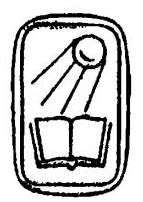
\includegraphics[max width=0.2\textwidth]{images/bo_d547imjef24c73bgfcdg_0_316_1786_143_202_0.jpg}
\end{center}
\hspace*{3em}

ИЗДАТЕЛЬСТВО «НАУКА»

ГЛАВНАЯ РЕДАКЦИЯ

ФИЗИКО-МАТЕМАТИЧЕСКОЙ ЛИТЕРАТУРЫ

МОСКВА 1969

518

П 56

УДК 519.9

Лев Семенович Понтрягин, Владимир Григорьевич Болтянский, Реваз Валерианович Гамкрелидзе, Евгений Фролович Мищенко

М., 1969 г., 384 стр. с илл.

Редактор Н. Х. Розов.

Техн. редактор С. Я. Шкляр.

Корректор Г. С. Иванова.

Сдано в набор 4/X 1968 г. Подписано к печати 3/III 1969 г. Бумага 84×108'/32. Физ. печ. л. 12. Условн. печ. л. 20,16. Уч.-изд. л. 18,66.

Тираж 21 500 экз. Т-02699. Цена книги 1 р. 40 к. Заказ № 140.

Издательство «Наука».

Главная редакция физико-математической литературы.

Москва, В-71, Ленинский проспект, 15

Оплена Трудового Красного Знамени Ленинградская типография Лб 1 «Печатный Двор» имени А. М. Горького Главполиграфпрома Комитета по печати при Совете Министров СССР, г. Ленинград, Гатчинская ул., 26. 2-2-3

81-69

оглавление

Предисловие ко второму изданию 5

Гда в а 1. Принцип максимума 13

1. Допустимые управления 13

2. Постановка основной задачи 15

3. Принцип максимума 23

4. Обсуждение принципа максимума 27

5. Примеры. Задача синтеза 28

6. Задача с подвижными концами и условия транс- версальности 52

7. Принцип максимума для неавтономных систем § 8. Задача с закрепленным временем 67

75

9. Связь принципа максимума с методом динамиче- ского программирования 79

\(\Gamma\) л а в а 2. Доказательство принципа максимума 84

§ 10. Допустимые управления 84

§ 11. Формулировка принципа максимума для произ- вольного класса допустимых управлений 88

§ 12. Система уравнений в вариациях и сопряженная ей система 92

13. Вариации управлений и траекторий 97

§ 14. Основные леммы 103

§ 15. Доказательство принципа максимума 111

§ 16. Вывод условий трансверсальности 121

Глава 3. Линейные оптимальные быстродействия 128

§ 17. Теоремы о числе переключений 128

18. Теоремы единственности 137

19. Теоремы существования 142

20. Синтез оптимального управления 152

21. Примеры 157

22. Моделирование линейных оптимальных быстро- действий при помощи релейных схем 189

§ 23. Линейные уравнения с переменными коэффици- ентами 199

\(\Gamma\) л а в а 4. Разные задачи 206

§ 24. Случай функционала, заданного несобетвенным интегралом 206

§ 25. Оптимальные процессы с параметрами 209

§ 26. Применение теории оптимальных процессов задачам приближения функций 215

§ 27. Оптимальные процессы с запаздыванием 233

§ 28. Одна задача преследования 247

\(\Gamma\) л а в а 5. Принцип максимума и вариационное исчисление 260

§ 29. Основная задача вариационного исчисления § 30. Задача Лагранжа 261 271

Гд а в а б. Оптимальные процессы при ограниченных фазо- вых координатах 281

§ 31. Постановка задачи 283

§ 32. Оптимальные траектории, лежащие на границе области 289

§ 33. Доказательство теоремы 22 (основные постро- ения) 295

34. Доказательство теоремы 22 (окончание) 316

35. Некоторые обобщения 324

§ 36. Условие скачка 326

37. Формулировка основного результата. Примеры. 337

Гда в а 7. Одна статистическая задача оптимального уп- равления 343

§ 38. Понятие о марковском процессе. Дифференциаль- ное уравнение Колмогорова 344

§ 39. Точная постановка статистической задачи 349

§ 40. Сведение вычисления функционала J к реше- нию краевой задачи для уравнения Колмогорова 351

41. Вычисление функционала J в случае, когда уравнение Колмогорова имеет постоянные ко- эффициенты 354

§ 42. Вычисление функционала J в общем случае 377

Литература 383

\section*{ПРЕДИСЛОВИЕ КО ВТОРОМУ ИЗДАНИЮ}

Физические процессы, имеющие место в технике, как правило у п р а в л я е м ы, т. е. могут осуществляться раз- личными способами в зависимости от воли человека.В связи с этим возникает вопрос о нахождении наилучшего в том или другом смысле или, как говорят, оптимального управления процессом. Речь может идти, например, об оптимальности в смысле быстродействия, т. е. о достижении цели процесса за кратчайшее время, о достижении этой цели с минимальной затратой энергии и т. п. Математически сформулированные, эти вопросы являются задачами в а - р и а ц и о н н о г о и с чи с л е н и я, которое и обязано им своим возникновением. В классическом вариационном ис- числении нет, однако, решения целого ряда вариацион- ных задач, важных для современной техники. Коллективу авторов этой книги принадлежит излагаемое здесь реше- ние значительного числа таких вариационных задач не- классического типа. Решение это в существенных чертах объединяется одним общим математическим приемом, ко- торый мы называем п р и н ц и п о м м а к с и м ум а.Сле- дует заметить, что все основные необходимые условия классического вариационного исчисления с обыкновен- ными производными следуют из принципа максимума (см. главу 5).

Мы рассматриваем здесь такие управляемые процессы, каждый из которых может быть описан системой обык- новенных дифференциальных уравнений

\[
\frac{d{x}^{i}}{dt} = {f}^{i}\left( {{x}^{1},\ldots ,{x}^{n},{u}^{1},\ldots ,{u}^{r}}\right) ,\;i = 1,2,\ldots ,n;(1 \tag{1}
\]

вдесь \({x}^{1},\ldots,{x}^{n}\) - величины, характеризующие процесс т. е. фазовые координаты управляемого объекта, опреде- ляющие его состояние в каждый момент времени t; \({u}^{1},\ldots,{u}^{r}\) — параметры управления, определяющие ход про- цесса, и t — время. Для того чтобы ход управляемого процесса (1) был определен на некотором отрезке времени \({t}_{0} \leq  t \leq  {t}_{1}\),достаточно, чтобы на этом отрезке времени были заданы (как функции времени) параметры управле- ния \({u}^{1},\ldots,{u}^{r}\) :

\[
{u}^{j} = {u}^{j}\left( t\right) ,\;j = 1,\ldots ,r. \tag{2}
\]

Тогда при заданных начальных значениях

\[
{x}^{i}\left( {t}_{0}\right)  = {x}_{0}^{i},\;i = 1,\ldots ,n, \tag{3}
\]

решение системы (1) определяется однозначно. Подлежащая решению вариационная задача, связанная с управляемым процессом (1), заключается в следующем. Рассматривается интегральный функционал

\[
J = {\int }_{{t}_{0}}^{{t}_{1}}{f}^{0}\left( {{x}^{1},\ldots ,{x}^{n},{u}^{1},\ldots ,{u}^{r}}\right) {dt} \tag{4}
\]

где \({f}^{0}\left( {{x}^{1},\ldots,{x}^{n},{u}^{1},\ldots,{u}^{r}}\right)  -\) заданная функция. Для каж- дого управления (2), заданного на некотором отрезке \({t}_{0} \leq  t \leq  {t}_{1}\),однозначно определяется ход управляемого про- цесса, и интеграл (4) принимает определенное значение. Допустим, что существуют управления (2), переводящие управляемый объект из заданного начального фазового состояния (3) в предписанное конечное фазовое состояние

\[
{x}^{i}\left( {t}_{1}\right)  = {x}_{1}^{i},\;i = 1,\ldots ,n. \tag{5}
\]

Требуется отыскать управление

\[
{\bar{u}}^{j}\left( t\right) ,\;j = 1,\ldots ,r, \tag{6}
\]

которое осуществляет переход управляемого объекта из состояния (3) в состояние (5) таким образом, чтобы функ- ционал (4) имел минимальное значение. При этом моменты времени б, и и в рассматриваемой постановке задачи не фиксируются, а требуется только, чтобы в начальный момент времени объект находился в состоянии (3), а в конечный момент — в состоянии (5) и чтобы функционал (4) достигал минимума. (Случай, когда моменты времени \({t}_{0},{t}_{1}\) фиксированы, также представляет интерес; он легко сводится к задачам, упоминаемым в этом введении, см. § 8.) В частном случае, когда функция \({f}^{0}\left( {{x}^{1},\ldots,{x}^{n},{u}^{1},\ldots,{u}^{r}}\right)\), определяющая функционал (4), тождественно равна едини- пе,функционал (4) имеет величину \({t}_{1} - {t}_{0}\),и наша вариа- ционная задача превращается в оптимальную задачу быст- родействия.

В технических задачах, где параметры управления \({u}^{1},\ldots,{u}^{r}\) определяют, например, положение рулей машины, эти параметры не могут принимать произвольных значе- ний, а подчинены некоторым ограничениям. По самому устройству описываемого системой (1) механизма параметр \({u}^{1}\) может, скажем, принимать лишь значения, удовлетво- ряющие условию

\[
\left| {u}^{1}\right|  \leq  1\text{ . } \tag{7}
\]

Или, например, если параметры и’ \({u}^{1}\), \({u}^{2}\) характеризуют векторную величину на плоскости, модуль которой не превосходит единицы, а направление произвольно, то эти параметры подчинены условию

\[
{\left( {u}^{1}\right) }^{2} + {\left( {u}^{2}\right) }^{2} \leq  1\text{ . } \tag{8}
\]

Вообще следует считать, что точка (и',..., и") должна принадлежать некоторому множеству И пространства с координатами \({u}^{1},\ldots,{u}^{r}\), причем выбор этого множества \(U\) отражает специфику объекта (1). Множество И. («область управления») в математической постановке задачи счи- тается произвольным, но для технических задач особенно важен и характерен случай з а м к н у т о г о множества И (cp. неравенства (7), (8)). Это условие означает, что для руля допустимы и его крайние положения (значения \({u}^{1} =  \pm  1\) в неравенстве (7) или граничные точки круга (8)), могущие, в частности, давать оптимальное управление. Именно это обстоятельство делает рассматриваемую вариа- ционную задачу неклассической, так как в классическом вариационном исчислении варьируемые параметры, не могут удовлетворять неравенствам типа (7), (8), включа- ющим и равенства.

Особенно ярко демонстрирует неклассический характер нашей вариационной задачи оптимальная задача по быстро- действию для системы (1), правые части которой являются л и н е й н ы м и функциями относительно переменных \({x}^{1},\ldots,{x}^{n},{u}^{1},\ldots,{u}^{r}\) c постоянными коэффициентами, а множество \(U\) представляет собой з а м к н у т ы й в ы - п у к л ы й м н о г о г р а н н и к, например куб, опреде- ляемый неравенствами:

\[
\left| {u}^{j}\right|  \leq  1,\;j = 1,\ldots ,r.
\]

В этом случае оказывается, что оптимальное управление (6) осуществляется точкой \(\left( {{u}^{1}\left( t\right),\ldots,{u}^{r}\left( t\right) }\right)\), поочередно находящейся в различных вершинах многогранника U. Правила, согласно которым управляющая точка перехо- дит скачками из одной вершины в другую, и дают закон оптимального управления. Эта линейная вариационная за- дача, имеющая важные технические приложения, решается на основе общих методов в главе 3. Классические же ме- тоды для решения такой задачи совершенно неприменимы.

Из сказанного о перескоках оптимально управляющей точки с вершины на вершину многогранника U следует, что класс допустимых управлений (2) нельзя считать состоящим из непрерывных функций. Мы предполагаем обычно, что он состоит из кусочно-непрерывных функций. Фазовые координаты и…, хг считаются непрерывными и кусочно-дифференцируемыми функциями времени. В этих предположениях необходимые условия оптимальности фор- мулируются в виде принципа максимума (см. главу 1), который доказывается в главе 2.

Если рассматриваемый объект представляет собой меха- ническую систему, то часть \({x}^{1},\ldots,{x}^{k}\) фазовых коорди- нат описывает ее геометрическое состояние, а часть \({x}^{k + 1},\ldots,{x}^{2k}\left( {{2k} = n}\right)\) -ee скорость. В некоторых задачах целью управляемого процесса в этом случае может быть не попадание объекта в определенную точку ( \({x}_{1}^{1},\ldots,{x}_{1}^{n}\) ) ф а в о в о г о пространства, а прибытие механической сис- темы в определенное пространственное поло- жение \(\left( {{x}_{1}^{1},\ldots,{x}_{1}^{h}}\right)\) при произвольных скоростях в конце процесса. Таким образом, здесь имеет место вариационная задача об оптимальном переходе объекта из определенной начальной точки и,..., х, фазового пространства в про- извольную точку к-мерной плоскости, определяемой уравнениями

\[
{x}^{1} = {x}_{1}^{1},\ldots ,{x}^{k} = {x}_{1}^{k}.
\]

Мы видим, что ранее сформулированная оптимальная задача не охватывает ряда важных проблем. Ввиду этого в \$ 6 главы 1 разбирается вопрос об оптимальном переходе объекта с некоторого начального многообразия \({M}_{0}\) точек фазового пространства на некоторое конечное многообразие \({M}_{1}\), \(\mathrm{n}\) ричем размерности многообразий Мо и М произвольны (в частности, когда они обе равны нулю, мы получаем первоначальную задачу).

Совершенно ясно, что не только управляющие пара- метры объекта, но и его фазовые координаты, по самому характеру технической задачи, должны иногда подчинять- ся некоторым ограничениям. Если, например, речь идет о движении самолета и и обозначает его высоту над землей, то должно быть выполнено неравенство \({x}^{1} \geq  \dot{h} > 0\), где h — минимальная допустимая высота полета. Неравен- ство из е новое не вытекает из свойств системы уравне- ний (1) и из неравенств, налагаемых на управляющие параметры, а является совершенно независимым. Задача об оптимальном управлении объектом, при котором изобра- жающая его точка фазового пространства должна все время оставаться в некоторой замкнутой области G фазо- вого пространства, решается в главе 6. Предполагается при этом, что область G имеет кусочно-гладкую границу. Движение объекта в этих условиях протекает частично внутри области G, подчиняясь там обычному принципу максимума, частично же по границе области G, подчиняясь там усложненному принципу максимума. Переходы от кусков траекторий, проходящих внутри G, к кускам траекторий, проходящим по границе области G, под- чиняются своеобразным правилам, напоминающим зако- ны преломления света и в некотором смысле обобща- ющим их.

До сих пор речь шла об оптимальном управлении, приводящем объект в заданную точку или на заданное подмногообразие фазового пространства.Задачей оптималь- ного управления может быть, однако, и задача об опти- мальном попадании в д в и ж у щ у ю с я точку фазового пространства. Допустим, что в фазовом пространстве имеется движущаяся точка

\[
{x}^{i} = {\theta }^{i}\left( t\right) ,\;i = 1,\ldots ,n. \tag{9}
\]

Тогда возникает задача об оптимальном приведении объ- екта (1) в совпадение с движущейся точкой (9). Эта за- дача легко сводится к рассмотренной. Достаточно ввести новые переменные, положив

\[
{y}^{i} = {x}^{i} - {\theta }^{i}\left( t\right) ,\;i = 1,\ldots ,n.
\]

В результате этого преобразования управляемая система (1) превращается в новую, правда, уже не автономную, а целью управляемого процесса становится приведение нового объекта ( \({y}^{1},\ldots,{y}^{n}\) ) в неподвижную точку (0,...,0) фазового пространства. Так как основные результаты легко распространяются и на не а в т о н о м н ы е управляе- мые процессы (см. \$ 7), то задача оказывается решенной.

Здесь мы считали, что движение преследуемой точки (9) определено заранее на протяжении всего рассмат- риваемого промежутка времени. Совершенно новый и практически важный вопрос возникает, когда движение преследуемого объекта не известно заранее, а сведения о нем поступают только с течением времени. Для того чтобы решать такую задачу о преследовании объекта, нужно иметь некоторые данные о его поведении. Весьма важным представляется случай, когда преследуемый объ- ект является управляемым, так что его движение описы- вается системой уравнений

\[
\frac{d{z}^{i}}{dt} = {g}^{i}\left( {{z}^{1},\ldots ,{z}^{n},{v}^{1},\ldots ,{v}^{s}}\right) ,\;i = 1,. \tag{10}
\]

Задача заключается в том, чтобы, зная технические воз- можности преследуемого объекта, т. е. систему уравнений (10), и его положение в каждый данный момент времени, определить управление преследующего объекта в тот же момент времени так, чтобы преследование осуществлялось оптимальным образом. В такой постановке задача рас- сматривается в теории дифференциальных игр, которая здесь не затрагивается. В главе 7 решается другая за- дача преследования. Предполагается, что в начальный момент положение преследуемого объекта известно, а дальнейшее его поведение описывается вероятностным образом, именно, процесс его движения считается марковс- ким. В этих предположениях ищется такое управление преследующего объекта (1), при котором встреча некото- рой малой окрестности объекта (1) с преследуемым объ- ектом является наиболее вероятной.

* *

За семь лет, прошедших с первого издания этой книги, принцип максимума оправдал себя, найдя многочислен- ные приложения. Поэтому уже здесь стоит остановиться в нескольких словах на его характере, происхождении и доказательстве. Для определенности ограничимся зада- чей быстродействия. Именно для этого случая принцип максимума был в качестве гипотезы высказан Л. С. Понт- рягиным.

Суть его заключается в следующем. Каждому допусти- мому управлению \({u}^{1}\left( t\right),\ldots,{u}^{r}\left( t\right)\),Заданному на отрезке \({t}_{0} \leq  t \leq  {t}_{1}\),и произвольному постоянному вектору ффа- зового пространства определенным образом ставится в со- ответствие функция

\[
H\left( {t,{u}^{1},\ldots ,{u}^{r}}\right)
\]

переменного \(t,{t}_{0} \leq  t \leq  {t}_{1}\),и допустимых управляющих параметров. Оказывается, что если взятое управление оптимально, то существует такое значение вектора ψ ≠0, что при каждом фиксированном значении \(t,{t}_{0} \leq  t \leq  {t}_{1}\), величина H, рассматриваемая как функция допустимых значений управляющих параметров, достигает своего мак- симума при \({u}^{j} = {u}^{j}\left( t\right),j = 1,\ldots,r\). Из этого видно, что, имея дело с принципом максимума, приходится сравнивать между собой не только близкие одно к другому управления. В этом его отличие от классических теорем вариационного исчисления, сила и некоторая трудность доказательства.

Первое доказательство принципа максимума было дано Р. В. Гамкрелидзе для линейных управляемых си- стем. Он же построил полную теорию этих систем. Идея его доказательства следующая: будем считать, что рас- сматриваемое оптимальное управление переводит точку \({x}_{0}\) в точку \({x}_{1}\). Если вместо оптимального управления взять произвольное допустимое управление, заданное на преж- нем отрезке, то оно переведет точку х, в некоторую точку \(x\left( {t}_{1}\right)\). Ввиду линейности совокупность всех получаемых так точек \(x\left( {t}_{1}\right)\) образует выпуклое тело P. Из оптималь- ности исходного управления вытекает, что точка хд ле- жит на границе этого тела. Таким образом, существует опорная плоскость к телу \(P\), проходящая через точку х, а вектор ψ, перпендикулярный к этой плоскости и на- правленный от тела P, и является тем, который исполь- зуется при построении функции H.

Для нелинейной управляемой системы множество всех точек \(x\left( {t}_{1}\right)\), получаемых с помощью всевозможных до- пустимых управлений, невыпукло и необозримо. Исполь- зование для линеаризации задачи управлений, мало отли- чающихся от оптимального управления, не соответствует характеру принципа максимума. В общем, нелинейном случае принцип максимума доказал В. Г. Болтянский, который вслед за тем построил основы нелинейной тео- рии оптимального управления. Именно, он удачно выб- рал класс управлений для сравнения с оптимальным, применив вариации Макшейна, т. е. рассмотрев те допу- стимые управления, которые отклоняются от оптималь- ного лишь на конечном числе малых интервалов времени, но на каждом интервале отклоняются произвольно. Этим самым задача была линеаризована: множество точек x (t,), соответствующих указанным управлениям, хотя и невыпукло, но близко к выпуклому, так что воз- никла возможность построения опорной плоскости и пер- пендикулярного к ней вектора ф.

Л. Понтрягин

\section*{ПРИНЦИП МАКСИМУМА}

\section*{§ 1. Допустимые управления}

Мы будем рассматривать поведение объекта, состояние которого в каждый момент времени характеризуется n действительными числами \({x}^{1},{x}^{2},\ldots,{x}^{n}\) (например, коор- динатами и скоростями). Векторное пространство X век- торной переменной \(x = \left( {{x}^{1},\ldots,{x}^{n}}\right)\) является фазовым пространством рассматриваемого объекта. Поведение (дви- жение) объекта заключается (с математической точки Зрения) в том, что переменные \({x}^{1},\ldots,{x}^{n}\) меняются с течением времени. Предполагается, что движением объ- екта можно у п р а в л я т ь, т. е. что объект снабжен некоторыми «рулями», от положения которых зависит движение объекта. Положения «рулёй» характеризуются точками и некоторой области управления U, которая может быть любым множеством некоторого r-мерного евклидова пространства \({E}_{r};3\) адание точки \(u = \left( {{u}^{1},{u}^{2},\ldots,{u}^{r}}\right)  \in  U\) равносильно заданию системы числовых параметров \({u}^{1},{u}^{2},\ldots,{u}^{r}\). В приложениях важен случай, когда U является з а м к н у т о й областью пространства E,. В ча- стности, область управления U может быть кубом r-мер- ного пространства переменных \({u}^{1},{u}^{2},\ldots,{u}^{r}\) :

\[
\left| {u}^{j}\right|  \leq  1,\;j = 1,2,\ldots ,r, \tag{1}
\]

или каким-либо другим замкнутым ограниченным мно- жеством этого r-мерного пространства. Физический смысл рассмотрения замкнутой и ограниченной (в пространстве переменных и", и",..., и") области управления Й ясен: управляющими параметрами \({u}^{1},{\dot{u}}^{2},\ldots,{u}^{r}\) могут служить количество подаваемого в двигатель топлива, температура, сила тока, напряжение и т. п., которые не могут при- нимать сколь угодно больших значений. Кроме того, в силу технической конструкции управляющей части объекта, между управляющими параметрами \({u}^{1},{u}^{2},\ldots,{u}^{r}\) могут существовать связи, выражаемые одним или не- сколькими уравнениями вида φ (и*, и*, и*) = 0. В этом случае область управления \(U\) может геометрически иметь более или менее сложный характер. Если, например, имеются два управляющих параметра и", и*, которые в силу конструкции объекта имеют вид и" = cos φ, и = sin φ, где φ — некоторый (произвольно задаваемый) угол, то областью управления будет окружность

\[
{\left( {u}^{1}\right) }^{2} + {\left( {u}^{2}\right) }^{2} = 1\text{ . } \tag{2}
\]

В дальнейшем мы просто будем говорить об области управления \(U\) и ее точках и ес U и будем представлять себе \(U\) в виде некоторого множества в пространстве пере- менных \({u}^{1},{u}^{2},\ldots,{u}^{r}\), считая его «точкой» и произволь- ную входящую в U систему управляющих параметров \(u = \left( {{u}^{1},{u}^{2},\ldots,{u}^{r}}\right)\) (см.,например,(1) или (2)).

Каждую.функцию \(u = u\left( t\right)\), определенную на некото- ром отрезке \({t}_{0} \leq  t \leq  {t}_{1}\) времени t и принимающую значе- ния в области управления \(U\),мы будем называть управ- лением. Так как И есть множество в пространстве управ- ляющих параметров и", и",..., и", то каждое управление

\[
u\left( t\right)  = \left( {{u}^{1}\left( t\right) ,{u}^{2}\left( t\right) ,\ldots ,{u}^{r}\left( t\right) }\right)
\]

является в е к т о р - ф у н к ц и е й (заданной на отрезке \({t}_{0} \leq  t \leq  {t}_{1}\) ), значения которой лежат в области управле- ния U. В дальнейшем, в зависимости от характера по- ставленной задачи, мы будем накладывать на управле- ние \(u\left( t\right)\) различные условия (кусочной непрерывности, кусочной дифференцируемости и т. п.). Управления, удовлетворяющие этим условиям, будем называть д о π y - с т и мы м и у п р а в л е н и я м и. В этой главе мы бу дем считать допустимыми управлениями произвольные кусочно-непрерывные управления (созначе- ниями в области управления U), т. е. такие управления \(u = u\left( t\right),\) каждое из которых непрерывно для всех рассмат- риваемых t, за исключением лишь конечного числа момен- тов времени, где функция \(u\left( t\right)\) может терпеть разрывы первого рода. Во избежание недоразумений отметим, что, по определению разрывов первого рода, в точке разрыва \(\tau\) предполагается существование к о н е ч н ы х пределов

\[
u\left( {\tau  - 0}\right)  = \mathop{\lim }\limits_{\substack{{t \rightarrow  \tau } \\  {t < \tau } }}u\left( t\right) ,\;u\left( {\tau  + 0}\right)  = \mathop{\lim }\limits_{\substack{{t \rightarrow  \tau } \\  {t > \tau } }}u\left( t\right) .
\]

Из этого, в частности, следует, что всякое управление и (t) ограничено (даже если область U не является ограничен- ной).

Значение кусочно-непрерывного управления \(u\left( t\right)\) в точке разрыва не играет сколько-нибудь существенной роли в дальнейшем. Однако для определенности нам удобно предполагать, что в каждой точке разрыва τ значение управления \(u\left( t\right)\) равно п р е д е л у с л е в а:

\[
u\left( \tau \right)  = u\left( {\tau  - 0}\right) , \tag{3}
\]

и что каждое рассматриваемое управление \(u\left( t\right)\) непре- рывно в концах отрезка \({t}_{0} \leq  t \leq  {t}_{1}\),на котором оно задано.

Итак, допустимым управлением мы условимся в этой главе называть всякую кусочно-непрерывную функцию \(u\left( t\right),{t}_{0} \leq  t \leq  {t}_{1}\), co значениями в области управления \(U\), удовлетворяющую условию (3) в точках разрыва и непре- рывную в концах отрезка \({t}_{0} \leq  t \leq  {t}_{1}\),на котором она задана. Кусочно-непрерывные управления соответствуют предположению о «безынерционности» рулей, так как значения функции и (t) могут (в момент разрыва) мгно- венно перескакивать из одной точки области управления в другую. Этот класс допустимых управлений, по-види- мому, наиболее интересен для технических применений развиваемой здесь теории.

\section*{§ 2. Постановка основной задачи}

Мы будем предполагать, что закон движения объекта (и закон воздействия «рулей» на это движение) записы- вается в виде системы дифференциальных уравнений

\[
\frac{d{x}^{i}}{dt} = {f}^{i}\left( {{x}^{1},{x}^{2},\ldots ,{x}^{n},{u}^{1},\ldots ,{u}^{r}}\right)  = {f}^{i}\left( {x,u}\right) ,
\]

\[
i = 1,2,\ldots ,n, \tag{4}
\]

или, в векторной форме,

\[
\frac{dx}{dt} = f\left( {x,u}\right) , \tag{5}
\]

где \(f\left( {x,u}\right)\) - вектор с координатами

\[
{f}^{1}\left( {x,u}\right) ,{f}^{2}\left( {x,u}\right) ,\ldots ,{f}^{n}\left( {x,u}\right) .
\]

Функции f’ определены для любых значений векторной переменной хеХ и для значений и, принадлежащих области управления U. Они предполагаются непрерыв- ными по совокупности переменных \({x}^{1},\;{x}^{2},\;\ldots,\;{x}^{n},\;u\) и непрерывно дифференцируемыми по \({x}^{1},{x}^{2},\ldots,{x}^{n}\). Иначе говоря, функции

\[
{f}^{i}\left( {{x}^{1},{x}^{2},\ldots ,{x}^{n},u}\right) \;\mathbf{u}\;\frac{\partial {f}^{i}\left( {{x}^{1},{x}^{2},\ldots ,{x}^{n},u}\right) }{\partial {x}^{j}};
\]

\[
i,j = 1,2,\ldots ,n,
\]

определены и непрерывны на прямом произведении \(X \times  U\).

Заметим, что система (4) автономна, т. е. правые ее части не зависят явно от времени t. Случай, когда правые части зависят от t, мы обсудим ниже (см. § 7).

Если задан закон управления, т. е. выбрано некото- рое допустимое управление и = и (t), то уравнение (5) принимает вид

\[
\frac{dx}{dt} = f\left( {x,u\left( t\right) }\right) , \tag{6}
\]

откуда (при любых начальных условиях х (t, 0) = х0) одно- значно определяется закон движения объекта \(x = x\left( t\right)\), т. e. решение уравнения (6), определенное на некотором отрезке времени. Именно, если управление и (t) задано на отрезке б 10 я 10 ты шне 11 ма (первого рода), причем и с <0 < < 0 <... < 0 h < t, то мы рассмотрим сначала уравнение (6) на отрезке б, с 4 с 4 где оно имеет непрерывную правую часть. Обозначим через \(x\left( t\right)\) ретение этого уравнения с начальным усло- вием \(x\left( {t}_{0}\right)  = {x}_{0}\). Если это решение определено на всем отрезке \({t}_{0} \leq  t \leq  {\theta }_{1}\) и имеет в точке 0,1 значение \(x\left( {\theta }_{1}\right)\),то мы можем рассмотреть уравнение (6) на отрезке 0, \textbackslash \textbackslash \textbackslash \textbackslash Second, воспользовавшись начальным значением x ( \({\theta }_{1}\) ). Это репе- ние также обозначим через x (t). Таким образом, построен- ное решение \(x\left( t\right)\) непрерывно во всех точках своего опре- деления и, в частности, в «точке сопряжения» 0,. Если теперь решение \(x\left( t\right)\) определено на всем отрезке \({t}_{0} \leq  t \leq  {\theta }_{2}\) и имеет в точке \({\theta }_{2}\) значение \(x\left( {\theta }_{2}\right)\), то мы можем рас- смотреть уравнение (6) на отрезке 6, с 10, с 10, с особыть и оде-но зовавшись начальным значением x ( 0, x 1, h. l. h. Получен- ное таким образом решение x (t) уравнения (6) является непрерывным и кусочно-дифференцируемым; именно, во всех точках,кроме \({\theta }_{1},{\theta }_{2},\ldots,{\theta }_{h}\), ретение \(x\left( t\right)\) (там,где оно определено) является непрерывно дифференцируемым. По- строенное решение x (t) мы будем называть решением сис- темы (4) (или уравнения (5)), соответствующим управле- нию \(u\left( t\right)\) при начальном условии \(x\left( {t}_{0}\right)  = {x}_{0}\). Это решение может не быть определено на всем отрезке \({t}_{0} \leq  t \leq  {t}_{1}\) задания управления \(u\left( t\right)\) (оно может уйти в бесконеч- ность).

Мы будем говорить, что допустимое управление и (t), \({t}_{0} \leq  t \leq  {t}_{1}\), переводит фазовую точку из положения \({x}_{0}\) в по- ложение \({x}_{1}\), если соответствующее ему решение \(x\left( t\right)\) урав- нения (5) (или, что то же, (6)),удовлетворяющее начальному условию \(x\left( {t}_{0}\right)  = {x}_{0}\), определено на всем отрезке б, и проходит в момент \({t}_{1}\) через точку \({x}_{1}\),т. e. удовлетво- ряет также конечному условию \(x\left( {t}_{1}\right)  = {x}_{1}\).

Предположим теперь, что задана еще одна функция \({f}^{0}\left( {{x}^{1},{x}^{2},\ldots,{x}^{n},u}\right)  = {f}^{0}\left( {x,u}\right)\), определенная и непрерывная вместе с частными производными \(\frac{\partial {f}^{0}}{\partial {xi}},\;i = 1,2,\ldots,n\), на всем пространстве X X U. Тогда основная задача (отыскание оптимальных управлений) может быть сфор- мулирована следующим образом.

\(B\) фазовом пространстве \(X\) даны две точки \({x}_{0}u{x}_{1}\) . Cpeди всех допустимых управлений и = и (t), переводящих фазовую точку из положения х, в положение х, (если такие управления существуют), найти такое, для которого функционал

\[
J = {\int }_{{t}_{0}}^{{t}_{1}}{f}^{0}\left( {x\left( t\right) ,u\left( t\right) }\right) {dt} \tag{7}
\]

\(x\left( t\right)\) — решение уравнения (5) с начальным условием \(x\left( {t}_{0}\right)  = {x}_{0}\) , coответствующее управлению \(u\left( t\right)\) , a \({t}_{1} -\) момент прохождения этого решения через точку \({x}_{1}\) .

Отметим, что (при фиксированных \({x}_{0},{x}_{1}\) ) верхний и нижний пределы б, и, в интеграле (7) не являются фиксированными числами, а зависят от выбора управ- ления и (t), переводящего фазовую точку из положе- ния \({x}_{0}\) в положение \({x}_{1}\) (эти пределы определяются из соотношений \(x\left( {t}_{0}\right)  = {x}_{0},x\left( {t}_{1}\right)  = {x}_{1})\). O решении задачи для случая закрепленных пределов мы будем говорить ниже (см. § 8).

Управление и (t), дающее решение поставленной выше задачи, называется оптимальным управлением, соответ- ствующим переходу из положения х, в положение х, а соответствующая траектория \(x\left( t\right)\) — оптимальной траек- торией. Таким образом, основная задача заключается в отыскании оптимальных управлений (и соответствую- щих оптимальных траекторий).

Важным частным случаем поставленной выше опти- мальной задачи является случай, когда

\[
{f}^{0}\left( {x,u}\right)  \equiv  1.
\]

B этом случае функционал (7) принимает вид:

\[
J = {t}_{1} - {t}_{0} \tag{8}
\]

и оптимальность управления и (t) означает минимальность времени перехода из положения \({x}_{0}\) в положение х. Задачу отыскания оптимальных управлений (и траекторий) в этом случае мы будем называть задачей об опти- мальном быстродейстродействии.

Для формулировки и доказательства необходимого усло- вия оптимальности нам будет удобно дать иную форму- лировку поставленной выше задачи. Именно, добавим к фа- зовым координатам \({x}^{1},{x}^{2},\ldots,{x}^{n}\),меняющимся по зако- ну (4), eme одну координату \({x}^{0}\),закон изменения которой имеет вид

\[
\frac{d{x}^{0}}{dt} = {f}^{0}\left( {{x}^{1},{x}^{2},\ldots ,{x}^{n},u}\right) ,
\]

где бу — функция, участвующая в определении функцио- нала J (см. (7)). Иначе говоря, мы будем рассматривать систему дифференциальных уравнений

\[
\frac{d{x}^{i}}{dt} = {f}^{i}\left( {{x}^{1},{x}^{2},\ldots ,{x}^{n},{u}^{1},\ldots ,{u}^{r}}\right)  \equiv  {f}^{i}\left( {x,u}\right) ,
\]

\[
i = 0,1,2,\ldots ,n, \tag{9}
\]

правые части которой не зависят от переменного \({x}^{0}\). Вводя в рассмотрение вектор

\[
x = \left( {{x}^{0},{x}^{1},{x}^{2},\ldots ,{x}^{n}}\right)  = \left( {{x}^{0},x}\right)
\]

\(\left( {n + 1}\right)\) -мерного векторного пространства X, мы можем систему (9) переписать в векторной форме

\[
\frac{dx}{dt} = f\left( {x,u}\right) , \tag{10}
\]

где \(f\left( {x,u}\right)\) - вектор пространства \(X\),имеющий коорди- наты \({f}^{0}\left( {x,u}\right),\ldots,{f}^{n}\left( {x,u}\right)\). Заметим,что вектор \(f\left( {x,u}\right)\) не зависит от координаты хов вектора х.

Пусть теперь и (t) — некоторое допустимое управление, переводящее \({x}_{0}\) в \({x}_{1}\), a \(x = x\left( t\right)\) — соответствующее реше- ние уравнения (5) с начальным условием x (t, 0) = x, 0 60- значим через х, то точку (0, x), т. е. точку пространства X, имеющую координаты 0, \({x}_{0}^{1},\ldots,{x}_{0}^{n}\),где \({x}_{0}^{1},\ldots,{x}_{0}^{n}\) - координаты точки \({x}_{0}\) в пространстве X. Тогда ясно, что решение уравнения (10), соответствующее управлению \(u\left( t\right)\), c начальным условием \(x\left( {t}_{0}\right)  = {x}_{0}\) определено на всем orpeake \({t}_{0} \leq  t \leq  {t}_{1}\) it immer bit

\[
{x}^{0} = {\int }_{{t}_{0}}^{t}{f}^{0}\left( {x\left( t\right) ,u\left( t\right) }\right) {dt}
\]

\[
x = x\left( t\right)
\]

В частности,при \(t = {t}_{1}\) мы получим

\[
{x}^{0} = {\int }_{{t}_{0}}^{{t}_{1}}{f}^{0}\left( {x\left( t\right) ,u\left( t\right) }\right) {dt} = J,\;x = {x}_{1},
\]

т. e. ретение \(x\left( t\right)\) уравнения (10) с начальным условием \(x\left( {t}_{0}\right)  = {x}_{0}\) проходит при \(t = {t}_{1}\) через точку \(x = \left( {J,{x}_{1}}\right)\). Иначе говоря, обозначив через П прямую линию, проходящую в пространстве X через точку х = (0, x, 1) па- раллельно оси хо (эта прямая П образована всеми точками \(\left( {\xi,{x}_{1}}\right)\),где число ξ произвольно; рис. 1),мы можем сказать, что решение \(x\left( t\right)\) проходит в момент \(t = {t}_{1}\) через точку, лежащую на прямой П и имеющую координату х0-е J. Обратно, если и (t) — такое допустимое управление, что соответствующее ему решение \(x\left( t\right)\) уравнения (10) с на- чальным условием \(x\left( {t}_{0}\right)  = {x}_{0} = \left( {0,{x}_{0}}\right)\) проходит в некото- рый момент \({t}_{1}\) через точку \({x}_{1} \in  \Pi\) c координатой \({x}^{0} = J\), то управление \(u\left( t\right)\) переводит (в пространстве Х) фазовую точку из положения \({x}_{0}\) в положение \({x}_{1}\),причем функцио- нал (7) принимает значение J.

\begin{center}
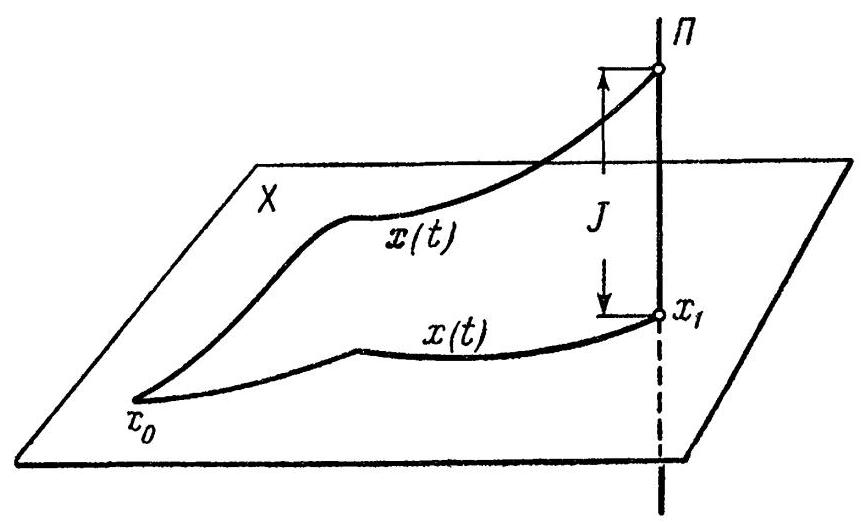
\includegraphics[max width=0.7\textwidth]{images/bo_d547imjef24c73bgfcdg_19_340_711_865_524_0.jpg}
\end{center}
\hspace*{3em}

Purc. 1.

Таким образом, мы можем сформулировать поставлен- ную выше оптимальную задачу в следующем эквивалент- ном виде.

\(B\left( {n + 1}\right)\) -мерном фазовом пространстве X даны точка \({x}_{0} = \left( {0,{x}_{0}}\right) u\) npямая \(\Pi\) , napаллельная ocu x \({}^{0}u\) npoxoдя- щая через точку (0, х, ). Среди всех допустимых управле- ний \(u = u\left( t\right)\) , oбладающих тем свойством,что соответ- ствующее решение xt() уравнения (10) с начальным усло- вием x( \({t}_{0}\) ) = x。nepeceкaem прямую П, найти такое, для которого точка пересечения с прямой П имеет наимень- шую координату хо.

Эту задачу мы и будем решать. Термины «оптималь- ное управление» и «оптимальная траектория» мы сохраним и для задачи в этой новой формулировке.

Отметим некоторые простые свойства оптимальных управлений и траекторий, непосредственно вытекающие из формулировки основной задачи. Прежде всего, из авто- номности системы (9) -вытекает, что при сдвиге вдоль оси t (рис. 2) свойства управлений не меняются. Иначе говоря, если управление \(u\left( t\right),{t}_{0} \leq  t \leq  {t}_{1}\),переводит фазо- вую точку из положения \({x}_{0}\) в положение \({x}_{1}\) и придает функционалу (7) значение \(J\), то при любом действитель- ном h управление \(u\left( {t + h}\right),{t}_{0} - h \leq  t \leq  {t}_{1} - h\), гаκже пе- реводит фазовую точку из положения \({x}_{0}\) в положение \({x}_{1}\) и придает функционалу (7) то же значение J. Это позволя- ет перемещать начальную точку \({t}_{0}\) отрезка б, \(\leq  t \leq  {t}_{1}\),на ко- тором задано управление \(u\left( t\right)\),в любую точку оси времени.

\begin{center}
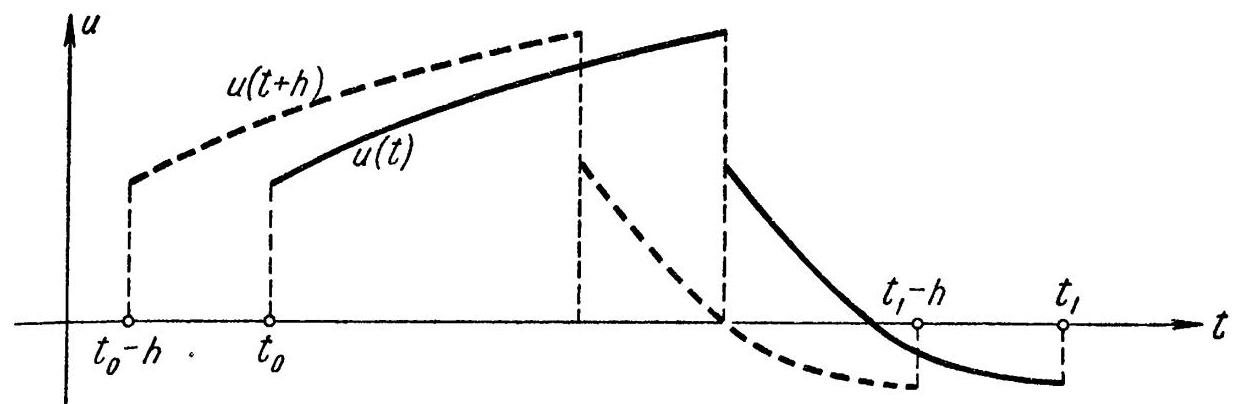
\includegraphics[max width=1.0\textwidth]{images/bo_d547imjef24c73bgfcdg_20_140_725_1245_404_0.jpg}
\end{center}
\hspace*{3em}

Pnc 2.

Далее, если \({x}_{0},{x}_{1},\ldots,{x}_{k}\) - конечная система точек фазового пространства X и если существует управление \({u}_{i}\left( t\right)\), переводящее фазовую точку из положения \({x}_{i - 1}\) в положение \({x}_{i}\) и придающее функционалу (7) значение \({J}_{i},i = 1,\ldots,k\), ro существует управление \(u\left( t\right)\),переводящее фазовую точку из положения \({x}_{0}\) в положение \({x}_{k}\) и при- дающее функционалу (7) значение \({J}_{1} + {J}_{2} + \ldots  + {J}_{k}\). В самом деле, в силу возможности сдвигать управления вдоль оси времени, мы можем считать, что отрезки, на которых определены управления \({u}_{i}\left( t\right)\),непосредственно примыкают один к другому (рис. 3), т. е. что управление \({u}_{i}\left( t\right)\) задано на отрезке \({t}_{i - 1} \leq  t \leq  {t}_{i}\),где \({t}_{0} < {t}_{1} < \ldots  < {t}_{k}\). Обозначим через и (t) управление, заданное на отрезке \({t}_{0} \leq  t \leq  {t}_{k}\) и совпадающее на полуинтервале \({t}_{i - 1} < t \leq  {t}_{i}\) c управлением \({u}_{i}\left( t\right)\),т. e. «объединение» всех управлений \({u}_{i}\left( t\right)\). Непосредственно проверяется, что управление \(u\left( t\right)\) переводит фазовую точку из положения \({x}_{0}\) в положение \({x}_{k}\) и придает функционалу (7) значение \({J}_{1} + {J}_{2} + \ldots  + {J}_{k}\). Заметим, что указанная операция «объединения» несколь- ких управлений была бы невозможна в классе н е п р е - ры в н ы х управлений (ибо в точках и, и, исп- построенное управление \(u\left( t\right)\) может иметь разрывы первого рода, даже если управления \({u}_{i}\left( t\right)\) были непрерывными; puc. 3).

\begin{center}
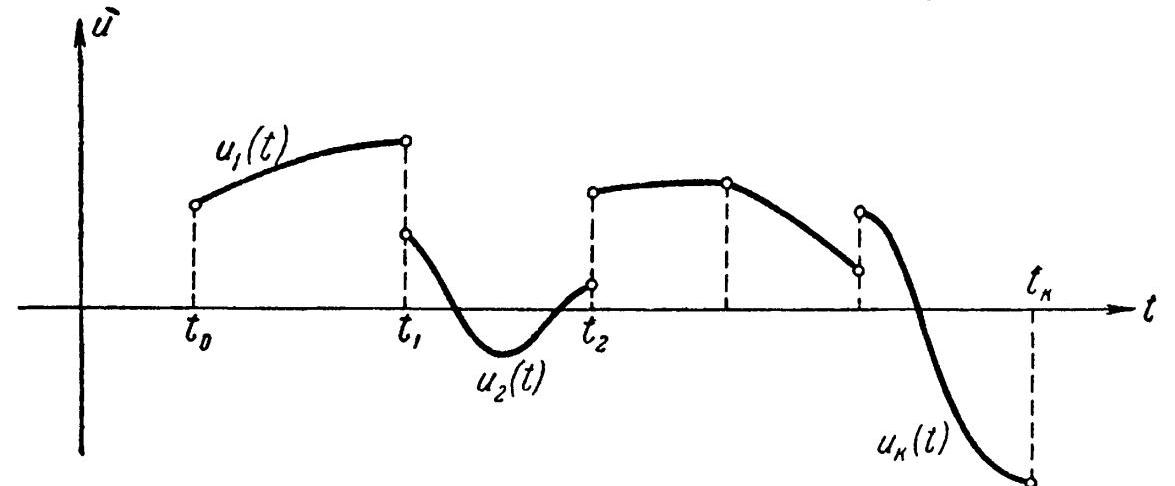
\includegraphics[max width=1.0\textwidth]{images/bo_d547imjef24c73bgfcdg_21_176_409_1175_486_0.jpg}
\end{center}
\hspace*{3em}

Pnc. 3.

Из сказанного выше легко следует, что всякий кусок оптимальной траектории также является оптимальной траекторией (и аналогично для оптимальных управле- ний). Более точно, пусть \(u\left( t\right),{t}_{0} \leq  t \leq  {t}_{1}, -\) оптималь - ное управление, соответст- вующее переходу из поло- жения \({x}_{0}\) в положение \({x}_{1}\), а \(x\left( t\right)  -\) соответствующая оптимальная траектория. Тогда, если \({t}_{0} \leq  {\tau }_{0} \leq  {\tau }_{1} \leq  {t}_{1}\), то управление \(u\left( t\right)\), рассматриваемое на отрезке \({\tau }_{0} \leq  t \leq  {\tau }_{1}\), является оптимальным управлением, соответствующим пе- реходу из положения \(x\left( {\tau }_{0}\right)\) в положение \(x\left( {\tau }_{1}\right)\), a \(x\left( t\right)\), \({\tau }_{0} \leq  t \leq  {\tau }_{1}\),является соответствующей оптимальной траекто- рией (рис. 4). В самом деле, обозначим значения интеграла (7),взятого по отрезкам \({t}_{0} \leq  t \leq  {\tau }_{0},{\tau }_{0} \leq  t \leq  {\tau }_{1},{\tau }_{1} \leq  t \leq  {t}_{1}\), соответственно через \({J}_{1},{J}_{2},{J}_{3}\). Тогда управление \(u\left( t\right)\), \({t}_{0} \leq  t \leq  {t}_{1}\), переводящее фазовую точку из положения \({x}_{0}\) в положение х, придает функционалу (7) значение \(J = {J}_{1} + {J}_{2} + {J}_{3}\). Если бы управление и (t), рассматривае- мое на отрезке то мету не было оптимальным, то суще- ствовало бы некоторое управление \(v\left( t\right)\),переводящее фа- зовую точку из положения \(x\left( {\tau }_{0}\right)\) в положение \(x\left( {\tau }_{1}\right)\) и прида- ющее функционалу (7) значение у метение у мету и по тогда мы по- лучили бы управление, переводящее фазовую точку из поло- жения \({x}_{0}\) в положение \({x}_{1}\) и придающее функционалу (7) значение \({J}_{1} + {J}_{2}^{\prime } + {J}_{3} < J\),что противоречит оптималь- ности управления \(u\left( t\right),{t}_{0} \leq  t \leq  {t}_{1}\).

\begin{center}
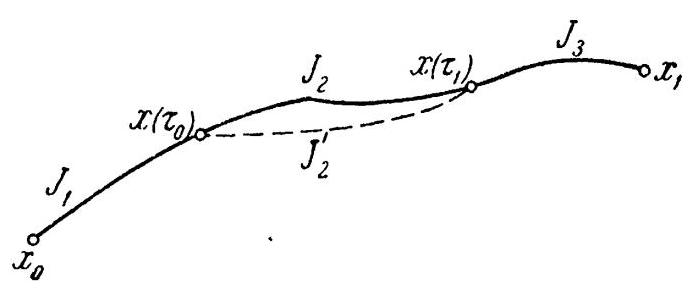
\includegraphics[max width=0.6\textwidth]{images/bo_d547imjef24c73bgfcdg_21_110_1295_693_292_0.jpg}
\end{center}
\hspace*{3em}

Puc. 4.

\section*{§ 3. Принцип максимума}

Переходим теперь к формулировке теоремы, дающей решение поставленной основной задачи. (Доказательство этой теоремы приведено во второй главе.) Для формули- ровки теоремы, кроме основной системы уравнений (9):

\[
\frac{d{x}^{i}}{dt} = {f}^{i}\left( {x,u}\right) ,\;i = 0,1,2,\ldots ,n, \tag{11}
\]

мы рассмотрим еще одну систему уравнений относительно вспомогательных (дополнительно рассматриваемых) пере- менных \({\psi }_{0},{\psi }_{1},\ldots,{\psi }_{n}\) :

\[
\frac{d{\psi }_{i}}{dt} =  - \mathop{\sum }\limits_{{\alpha  = 0}}^{n}\frac{\partial {f}^{\alpha }\left( {x,u}\right) }{\partial {x}^{i}}{\psi }_{\alpha },\;i = 0,1,\ldots ,n. \tag{12}
\]

Если мы выбрали некоторое допустимое управление \(u\left( t\right),{t}_{0} \leq  t \leq  {t}_{1}\),и имеем соответствующую фазовую траек- торию \(x\left( t\right)\) системы (11) с начальным условием x (t,0) = x0, то система (12) принимает вид

\[
\frac{d{\psi }_{i}}{dt} =  - \mathop{\sum }\limits_{{\alpha  = 0}}^{n}\frac{\partial {f}^{\alpha }\left( {x\left( t\right) ,u\left( t\right) }\right) }{\partial {x}^{i}}{\psi }_{\alpha },i = 0,1,\ldots ,n. \tag{13}
\]

Эта система линейна и однородна; поэтому при любых начальных условиях для фи она допускает единственное решение

\[
\psi  = \left( {{\psi }_{0},{\psi }_{1},{\psi }_{2},\ldots ,{\psi }_{n}}\right)
\]

(определенное на всем отрезке \({t}_{0} \leq  t \leq  {t}_{1}\),на котором опре- делены управление \(u\left( t\right)\) и траектория \(x\left( t\right)\) ). Как и ре- шение \(x\left( t\right)\) системы (11), ретение системы (13) состоит из непрерывных функций цы (н) имеющих всюду, кроме конечного числа точек (а именно, точек разрыва управ- ления \(u\left( t\right)\) ), непрерывные производные по \(t\). Всякое реше- ние системы (13) (при любых начальных условиях) мы будем называть решением системы (12), соответствую- щим выбранному управлению и (t) и фазовой траекто- рии \(x\left( t\right)\).

Мы теперь объединим системы (11), (12) одной записью, для чего рассмотрим следующую функцию Ж неремен- ных \({x}^{1},\ldots,{x}^{n},{\psi }_{0},{\psi }_{1},\ldots,{\psi }_{n},{u}^{1},\ldots,{u}^{r}\) :

\[
\mathcal{K}\left( {\psi ,x,u}\right)  = \left( {\psi ,f\left( {x,u}\right) }\right)  = \mathop{\sum }\limits_{{\alpha  = 0}}^{n}{\psi }_{\alpha }{f}^{\alpha }\left( {x,u}\right) .
\]

Непосредственно проверяется, что написанные выше систе- мы (11) и (12) могут быть с помощью этой функции Ж записаны в виде следующей гамильтоновой системы:

\[
\frac{d{x}^{i}}{dt} = \frac{\partial \mathcal{K}}{\partial {\psi }_{i}},\;i = 0,1,\ldots ,n, \tag{14}
\]

\[
\frac{d{\psi }_{i}}{dt} =  - \frac{\partial \mathcal{K}}{\partial {x}^{i}},\;i = 0,1,\ldots ,n. \tag{15}
\]

Итак, взяв произвольное допустимое (т. е. кусочно- непрерывное) управление \(u\left( t\right),{t}_{0} \leq  t \leq  {t}_{1}\),и начальное условие \(x\left( {t}_{0}\right)  = {x}_{0}\),мы можем найти соответствующую (т. e. удовлетворяющую системе (14)) траекторию \(x\left( t\right)  = \; = \left( {{x}^{0}\left( t\right),{x}^{1}\left( t\right),\ldots,{x}^{n}\left( t\right) }\right).\Pi\) Ocne этого мы можем нахо- дитъ coomeemcmøyòuyuē ěункциям и (t) и x (t) репения

\[
\psi \left( t\right)  = \left( {{\psi }_{0}\left( t\right) ,{\psi }_{1}\left( t\right) ,\ldots ,{\psi }_{n}\left( t\right) }\right)
\]

системы (15). Еще раз подчеркнем, что вектор-функции \(x\left( t\right)\) и \(\psi \left( t\right)\) непрерывны и всюду,кроме конечного числа точек, имеют непрерывные производные по t.

При фиксированных (постоянных) значениях ф и и функция Ж становится функцией параметра иСЕ ; точную верхнюю грань значений этой функции мы обозначим через \(\mathcal{M}\left( {\psi,x}\right)\) :

\[
\mathcal{M}\left( {\psi ,x}\right)  = \mathop{\sup }\limits_{{u \in  U}}\mathcal{K}\left( {\psi ,x,u}\right) .
\]

Если точная верхняя грань значений непрерывной функ- цип Ж д о с т и г а е т с я в некоторой точке области управления \(U\), то Ж (ф, х) есть максимум значений функ- ции Ж при фиксированных ф и х. Поэтому нижеследую- щую теорему 1 (необходимое условие оптимальности), главным содержанием которой является равенство (16), мы называем п р и н и и п о м м а к с и м у м а.

T e o p e m a 1. Пусть и (t), t, <em> мсто допус- тимое управление, что соответствующая ему траектория \(x\left( t\right) \left( {c \text{ м }.\left( {14}\right) }\right),u \sqsubset  {xc}\) ) square \(m\) then \({t}_{0}\) иЗп р о - к с т и ходит в момент \({t}_{1}\) через некоторую точку прямой П. Для оптимальности управления и(t) и траектории x (t) необходимо существование такой ненулевой непрерывной вектор-функции \(\psi \left( t\right)  = \left( {{\psi }_{0}\left( t\right),{\psi }_{1}\left( t\right),\ldots,{\psi }_{n}\left( t\right) }\right)\), соответ- ствующей функциям и(t) и х(t) (см. (15)), что:

\({1}^{ \circ  }\) npu любом \(t,{t}_{0} \leq  t \leq  {t}_{1},{\text{ ф }y}\) нкция \(\mathcal{K}\left( {\psi \left( t\right) ,x\left( t\right) ,u}\right)\) переменного \(u \in  U\) достигает в точке и = и (t) максимума

\[
\mathcal{K}\left( {\psi \left( t\right) ,x\left( t\right) ,u\left( t\right) }\right)  = \mathcal{M}\left( {\psi \left( t\right) ,x\left( t\right) }\right) ; \tag{16}
\]

\({2}^{ \circ  }\) в конечный момент \({t}_{1}\) выполнены соотношения

\[
{\psi }_{0}\left( {t}_{1}\right)  \leq  0,\mathcal{M}\left( {\psi \left( {t}_{1}\right) ,x\left( {t}_{1}\right) }\right)  = 0. \tag{17}
\]

Оказывается, далее, что если величины ψ (t), x (t), и (t) удовлетворяют системе (14), (15) и условию 1 \textdegree, то функ- ции \({\psi }_{0}\left( t\right) u\mathcal{M}\left( {\psi \left( t\right),x\left( t\right) }\right)\) переменного t являются посто- янными, так что проверку соотношений (17) можно проводить не обязательно в момент ны, а в любой мо- мент t, \({t}_{0} \leq  t \leq  {t}_{1}\). (Доказательство теоремы 1 приво- дится в гл. 2.)

Выведем теперь из теоремы 1 аналогичное необходимое условие для оптимальности по быстродействию. Для этого в теореме 1 следует положить \({f}^{0}\left( {x,u}\right)  = 1\). Функция Ж принимает в этом случае вид

\[
\mathcal{K} = {\psi }_{0} + \mathop{\sum }\limits_{{v = 1}}^{n}{\psi }_{v}{f}^{v}\left( {x,u}\right)
\]

Вводя п-мерный вектор \(\psi  = \left( {{\psi }_{1},{\psi }_{2},\ldots,{\psi }_{n}}\right)\) и функцию

\[
H\left( {\psi ,x,u}\right)  = \mathop{\sum }\limits_{{v = 1}}^{n}{\psi }_{v}{f}^{v}\left( {x,u}\right)
\]

мы можем записать уравнения (4) и (12) (кроме урав- нения (12) для \(i = 0\), которое теперь не нужно) в виде гамильтоновой системы

\[
\frac{d{x}^{i}}{dt} = \frac{\partial H}{\partial {\psi }_{i}},\;i = 1,2,\ldots ,n, \tag{18}
\]

\[
\frac{d{\psi }_{i}}{dt} =  - \frac{\partial H}{\partial {x}^{i}},i = 1,2,\ldots ,n. \tag{19}
\]

При фиксированных значениях ψ и х функция H становится функцией параметра и; верхнюю грань зна- чений этой функции мы обозначим через M (ψ, х):

\[
M\left( {\psi ,x}\right)  = \mathop{\sup }\limits_{{u \in  U}}H\left( {\psi ,x,u}\right) .
\]

B силу соотношения \(H\left( {\psi,x,u}\right)  = \mathcal{K}\left( {\psi,x,u}\right)  - {\psi }_{0}\) мы получаем

\[
M\left( {\psi ,x}\right)  = \mathcal{M}\left( {\psi ,x}\right)  - {\psi }_{0},
\]

и потому условия (16) и (17) принимают теперь вид

\[
H\left( {\psi \left( t\right) ,x\left( t\right) ,u\left( t\right) }\right)  = M\left( {\psi \left( t\right) ,x\left( t\right) }\right)  =  - {\psi }_{0} \geq  0.
\]

Таким образом, мы получаем следующую теорему.

T e o p e m a 2. Пусть и (t), t, 6 ≤ t ≤ t, — допустимое управление, переводящее фазовую точку из положения хо в положение \({x}_{1}\), a x \(\left( t\right)  -\) соответствующая траектория \(\left( {{cm}.\left( {18}\right) }\right)\), max что \(x\left( {t}_{0}\right)  = {x}_{0},x\left( {t}_{1}\right)  = {x}_{1}\). Для оптималь- ности (по быстродействию) управления и (t) и траектории \(x\left( t\right)\) необходимо существование такой ненулевой непре- рывной вектор-функции \(\psi \left( t\right)  = \left( {{\psi }_{1}\left( t\right),{\psi }_{2}\left( t\right),\ldots,{\psi }_{n}\left( t\right) }\right)\), соответствующей функциям и (t) и х (t) (см. (19)), что:

\({1}^{ \circ  }\) для всех t, \({t}_{0} \leq  t \leq  {t}_{1},{\phi y}{\mu }_{K{U}_{2}}H\left( {\psi \left( t\right) ,x\left( t\right) ,u}\right)\) ne- ременного \(u \in  U\) достигает в точке и = и (t) максимума

\[
H\left( {\psi \left( t\right) ,x\left( t\right) ,u\left( t\right) }\right)  = M\left( {\psi \left( t\right) ,x\left( t\right) }\right) ; \tag{20}
\]

\({2}^{ \circ  }\) в конечный момент \({t}_{1}\) выполнено соотношение

\[
M\left( {\psi \left( {t}_{1}\right) ,x\left( {t}_{1}\right) }\right)  \geq  0. \tag{21}
\]

Оказывается, далее, что если величины ψ (t), x (t), и (t) удовлетворяют системе (18), (19) и условию 1 \textdegree, то функ- ция \(M\left( {\psi \left( t\right),x\left( t\right) }\right)\) переменного \(t\) постоянна, man что проверку соотношения (21) можно проводить не обяза- тельно в момент \({t}_{1}\), a в любой момент t, \({t}_{0} \leq  t \leq  {t}_{1}\).

\section*{§ 4. Обсуждение принципа максимума *)}

Теорема 1 позволяет из всех траекторий, начинаю- щихся в точке х, и кончающихся в некоторой точке прямой П, и соответствующих им управлений выделить лишь отдельные, вообще говоря, изолированные траек- тории и управления, удовлетворяющие всем сформули- рованным условиям. Действительно, мы имеем 2n + 3 соотношений (14), (15), (16) между 2n + 3 переменными **) \({x}^{\alpha },{\psi }_{\alpha },u\),т. e. имеем «полную систему соотношений» для определения всех этих переменных. Так как, далее, соотношение (16) конечное (не дифференциальное), а диф- ференциальные уравнения мы имеем в количестве 2n + 2 (соотношения (14) и (15)), то решения системы уравне- ний (14), (15), (16) зависят, вообще говоря, от 2n + 2 параметров (начальных условий). Однако один из этих параметров является несущественным, так как функции \({\psi }_{a}\left( t\right)\) определены лишь с точностью до общего множи- теля (ибо функция Ж однородна относительно ф). Кроме того, один из параметров связан условием, что в момент \({t}_{0}\) величина

\[
\mathop{\max }\limits_{{u \in  U}}\mathcal{K}\left( {\psi \left( {t}_{0}\right) ,x\left( {t}_{0}\right) ,u}\right)
\]

обращается в нуль.

\HRule

*) Этот параграф имеет своей целью показать «достаточность» системы соотношений, указанной в теореме 1, для решения поставленной оптимальной задачи. Приводимые в этом параграфе рассуждения не претендуют на строгость и нигде в дальнейшем не используются.

**) Напомним, что «одна» переменная и может распадаться на несколько отдельных переменных, например может быть точ- кой r-мерного векторного пространства; в этом случае условие максимума (16) также можно считать содержащим r отдельных со- отношений. Если, например, максимум достигается во внутренней точке области управления U (расположенной в r-мерном простран- стве переменных и',... иг), то для выполнения условия макси- мума (16) необходимо обращение в нуль r частных производных:

\[
{\left. \frac{\partial \mathcal{K}\left( {\psi \left( t\right) ,x\left( t\right) ,u}\right) }{\partial {u}^{j}}\right| }_{u = u\left( l\right) } = 0,\;j = 1,\ldots ,r;
\]

если максимум достигается на (r—1)-мерной грани области управ- ления U, то должно выполняться условие принадлежности точки \(u\left( t\right)\) этой грани (это дает одно соотношение) и должны обра- щаться в нуль частные производные функции Ж (ф(t), х(t), и по всем направлениям в этой грани (это дает еще r — 1 coor- ношений). Аналогичное положение вещей имеет место и на гранях меньшего числа измерений (или на искривленных частях границы области управления U). Таким образом, во всех случаях можно считать, что если область управления U является r-мерной, то условие максимума (16) содержит r соотношений.

\HRule

Итак, все многообразие решений системы (14), (15), (16) зависит от \({2n}\) параметров. Этими 2n параметрами следует распорядиться так, чтобы траектория \(x\left( t\right)\) проходила при заданном \(t = {t}_{0}\) через точку х, a при к а к о м-н и б у д ь \({t}_{1} > {t}_{0}\) проходила через точку на пря- мой П. Число и Чи также является параметром, так что всего у нас имеется \({2n} + 1\) сутественных парамет- ров. Условие прохождения траектории через точку х, и прямую П дает 2n — 1 соотношений. Следовательно, можно ожидать, что имеются лишь отдельные, изолированные траектории, соединяющие точку х, с прямой П и удовле- творяющие условиям, указанным в теореме 1. Лишь эти отдельные, изолированные траектории и могут оказаться оптимальными (ибо указанные в теореме 1 условия н е - об х о д и м ы для оптимальности).

Если, в частности, условиям теоремы 1 удовлетво- ряет лишь о д н а траектория, соединяющая точку х, с точкой прямой П, а из технических соображений, приведших к постановке оптимальной задачи, «ясно», что оптимальная траектория должна существовать, то можно надеяться, что найденная траектория как раз и является оптимальной. Следует, однако, отметить, что математически вопрос о существовании оптимальной траектории представляется очень важным и трудным. В частном случае оптимальности по быстродействию для линейных систем (4) он решается в третьей главе.

\section*{§ 5. Примеры. Задача синтеза}

В этом параграфе мы рассмотрим применение прин- ципа максимума к решению некоторых простых задач об оптимальных быстродействиях. Из рассмотрения этих примеров выясняется новая важная постановка задачи об оптимальных процессах — задача синтеза оптимальных управлений. Пример 1

Рассмотрим уравнение д \(\frac{{d}^{2}x}{d{t}^{2}} = u\),где \(u\) - вещественный управляющий параметр, подчиненный условию |и| ≤1. В фазовых координатах \({x}^{1} = x,{x}^{2} = \frac{dx}{dt}\) это уравнение переписывается в виде следующей системы:

\[
\frac{d{x}^{1}}{dt} = {x}^{2},\;\frac{d{x}^{2}}{dt} = u. \tag{22}
\]

Рассмотрим (для фазовой точки, движущейся по за- кону (22)) задачу о быстрейшем попадании в начало координат (0, 0) из заданного начального состояния х,. Иначе говоря, мы будем рассматривать задачу об опти- мальном быстродействии в случае, когда конечным положением служит начало координат: \({x}_{1} = \left( {0,0}\right)\).

Функция H в рассматриваемом случае имеет вид

\[
H = {\psi }_{1}{x}^{2} + {\psi }_{2}u \tag{23}
\]

Далее, для вспомогательных переменных \({\psi }_{1},{\psi }_{2}\) мы полу- чаем систему уравнений (см. (19), (23))

\[
\frac{d{\psi }_{1}}{dt} = 0,\;\frac{d{\psi }_{2}}{dt} =  - {\psi }_{1},
\]

откуда \({\psi }_{1} = {c}_{1},{\psi }_{2} = {c}_{2} - {c}_{1}t\left( {{c}_{1},{c}_{2} - \text{ постоянные). Coor- }}\right)\) ношение (20) дает нам (учитывая (23) и условие \(- 1 \leq  u \leq  1)\)

\[
u\left( t\right)  = \operatorname{sign}{\psi }_{2}\left( t\right)  = \operatorname{sign}\left( {{c}_{2} - {c}_{1}t}\right) . \tag{24}
\]

Из (24) следует, что каждое оптимальное управ- ление и (t), ъ == сы хвляется кусочно-постоянной функ- цией, принимающей значения ±1 и имеющей не более двух интервалов постоянства ( \textbackslash t60 линейная функция \({c}_{2} - {c}_{1}t\) не более одного раза меняет знак на отрезке \({t}_{0} \leq  t \leq  {t}_{1})\). Обратно, любая такая функция \(u\left( t\right)\) может быть получена из соотношения (24) яри некоторых зна- чениях постоянных \({c}_{1},{c}_{2}\).

Для отрезка времени, на котором и ≡1, мы имеем (в силу системы (22))

\[
{x}^{2} = t + {s}^{2},{x}^{1} = \frac{{t}^{2}}{2} + {s}^{2}t + {s}^{1} = \frac{1}{2}{\left( t + {s}^{2}\right) }^{2} + \left( {{s}^{1} - \frac{{\left( {s}^{2}\right) }^{2}}{2}}\right)
\]

( \({s}^{1}\), \({s}^{2} -\) постоянные интегрирования), откуда получаем

\[
{x}^{1} = \frac{1}{2}{\left( {x}^{2}\right) }^{2} + s, \tag{25}
\]

где \(s = {s}^{1} - \frac{1}{2}{\left( {s}^{2}\right) }^{2} -\) постоянная. Таким образом, кусок фазовой траектории, для которого \(u \equiv  1\), представляет собой дугу параболы (25). Семейство парабол (25) пока- зано на рис. 5, а).

\begin{center}
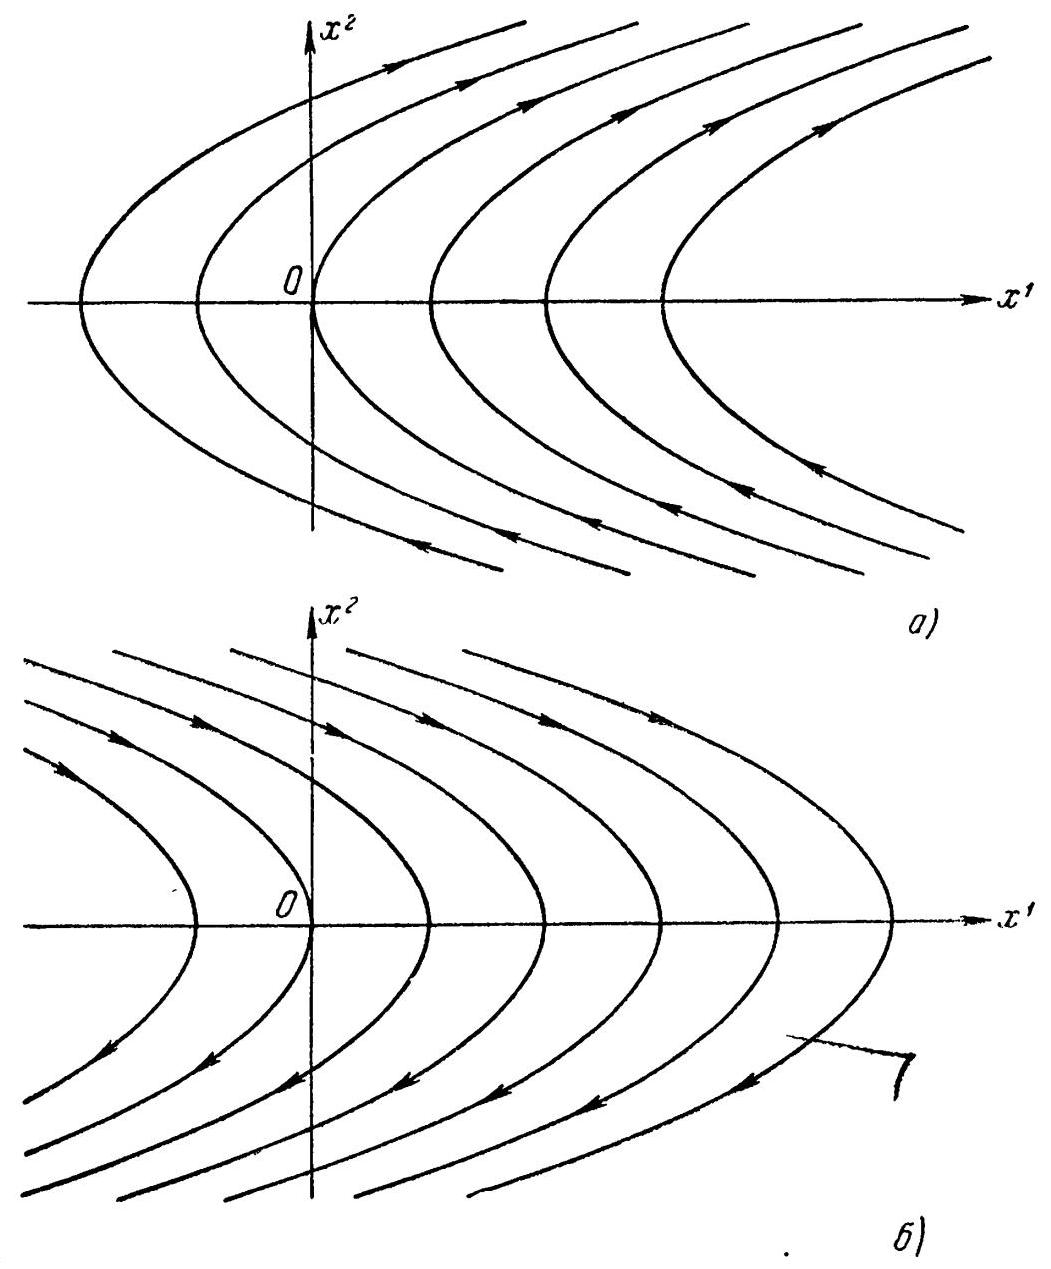
\includegraphics[max width=0.9\textwidth]{images/bo_d547imjef24c73bgfcdg_29_225_503_1051_1269_0.jpg}
\end{center}
\hspace*{3em}

Pnc. 5.

Аналогично, для отрезка времени, на котором и ≡ — 1, Mbl IMeeM

\[
{x}^{2} =  - t + {s}^{\prime 2}
\]

\[
{x}^{1} =  - \frac{{t}^{2}}{2} + {s}^{\prime 2}t + {s}^{\prime 1} =  - \frac{1}{2}{\left( -t + {s}^{\prime 2}\right) }^{2} + \left( {{s}^{\prime 1} + \frac{1}{2}{\left( {s}^{\prime 2}\right) }^{2}}\right) ,
\]

откуда получаем

\[
{x}^{1} =  - \frac{1}{2}{\left( {x}^{2}\right) }^{2} + {s}^{\prime }. \tag{26}
\]

Сетейство парабол (26) показано на рис. 5, 6). По пара- болам (25) фазовые точки движутся снизу вверх (ибо \(\frac{d{x}^{2}}{dt} = u =  + 1\) ), a по параболам (26) — сверху вниз

\[
\left( {\frac{d{x}^{2}}{dt} =  - 1}\right) .
\]

\begin{center}
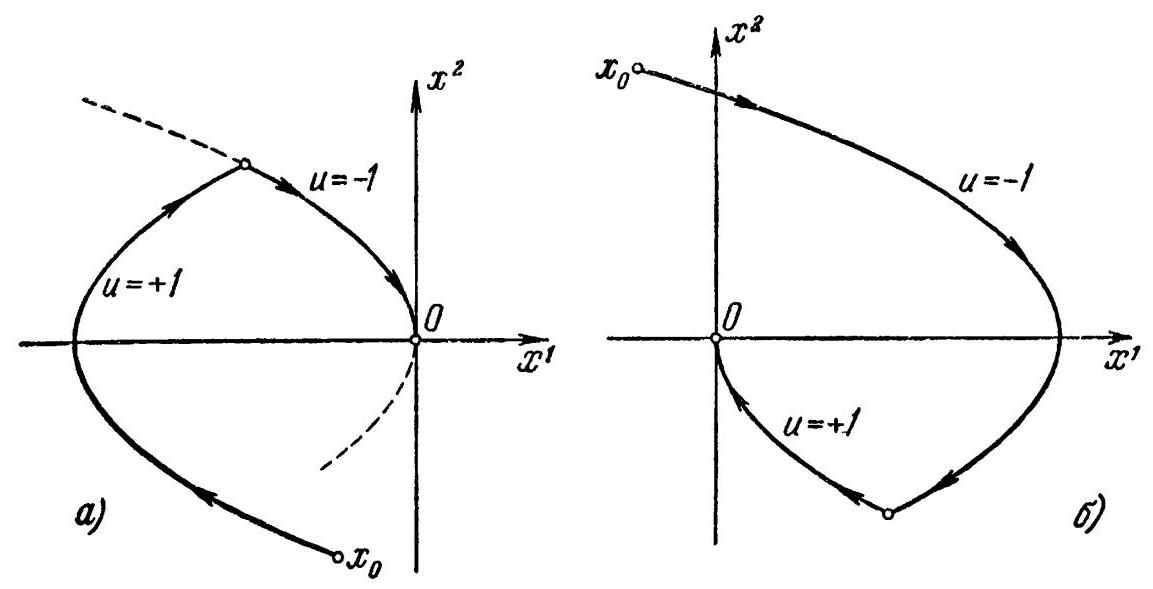
\includegraphics[max width=1.0\textwidth]{images/bo_d547imjef24c73bgfcdg_30_180_575_1153_589_0.jpg}
\end{center}
\hspace*{3em}

Puc. 6.

Как было указано выше, каждое оптимальное управ- ление \(u\left( t\right)\) является кусочно-постоянной функцией, при- нимающей значения ± 1 и имеющей не более двух интер- валов постоянства. Если управление и (t) сначала, в тече- ние некоторого времени, равно +1, а затем равно —1, то фазовая траектория состоит из двух кусков парабол (рис. 6, а)), примыкающих друг к другу, причем второй из этих кусков лежит на той из парабол (26), которая проходит через начало координат (ибо искомая траек- тория должна вести в начало координат). Если же, наоборот, сначала и е — 1, а затем и == 1, то фазовая кривая заменяется центрально симметричной (рис. 6, б)). На рис. 6 надписаны на дугах парабол соответствующие значения управляющего параметра и. На рис. 7 изобра- жено все семейство полученных таким образом фазовых траекторий (АО —дуга параболы \({x}^{1} = \frac{1}{2}{\left( {x}^{2}\right) }^{2}\), располо- женная в нижней полуплоскости; ВО — дуга параболы \({x}^{1} =  - \frac{1}{2}{\left( {x}^{2}\right) }^{2}\), расположенная в верхней полуплоскости). Фазовая точка движется по проходящей через начальную точку и дуге параболы (26), если точка хор располо- жена выше линии АОВ и по дуге параболы (25), если точка \({x}_{0}\) расположена ниже этой линии. Иначе говоря, если начальное положение \({x}_{0}\) расположено в ы ш е линии \({AOB}\), то фазовая точка должна двигаться под воздей- ствием управления \(u =  - 1\) до тех пор,пока она не по- падет на дугу АО; в момент попадания на дугу АО значение и переключается и становится равным +1 вплоть до момента попадания в начало координат. Если же начальное положение \({x}_{0}\) расположено н и ж е линии AOB, то и должно быть равно +1 до момента попадания на дугу BO, а в момент попадания на дугу BO значе- ние и переключается и становится равным —1.

\begin{center}
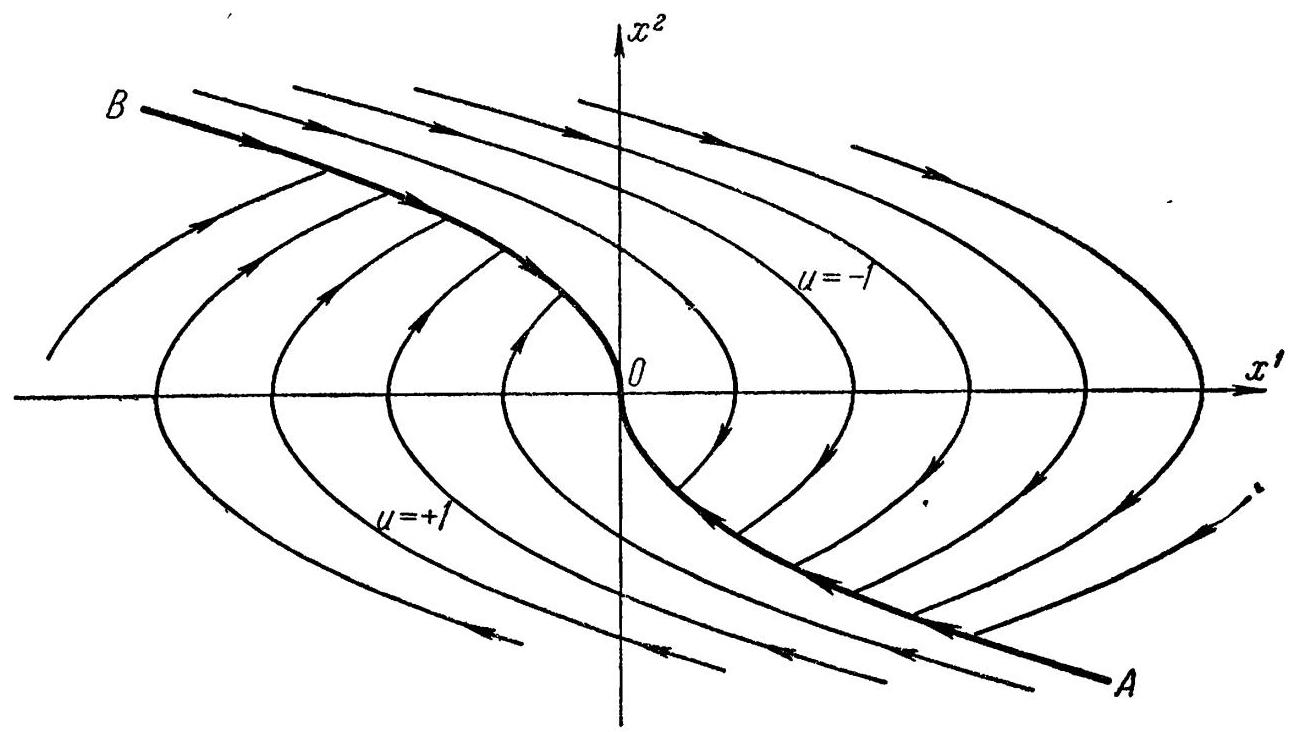
\includegraphics[max width=1.0\textwidth]{images/bo_d547imjef24c73bgfcdg_31_115_589_1298_732_0.jpg}
\end{center}
\hspace*{3em}

Pnc. 7.

Итак, согласно теореме 2, только описанные выше траектории могут быть оптимальными, причем из про- веденного исследования видно, что из каждой точки фазовой плоскости исходит т о л ь к о о д н а траектория, ведущая в начало координат, которая может быть опти- мальной (т. е. задание начальной точки \({x}_{0}\) однозначно определяет соответствующую траекторию). Если бы мы были уверены в том, что оптимальная траектория всегда (т. е. для любой начальной точки и, с у н е с т в у е т, то могли бы с уверенностью сказать, что все найденные тра- ектории являются оптимальными. В главе 3 мы сформу- лируем т е о р е м у с у щ е с т в о в а н и я для линейных систем оптимального быстродействия, из которой вытека- ет, в частности, что в рассматриваемом примере для лю- бой начальной точки х, существует оптимальная траекто- рия (см. стр. 142). Таким образом, найденные траектории (рис. 7) являются оптимальными, и других оптимальных траекторий, ведущих в начало координат, не существует.

Полученное в рассмотренном примере решение опти- мальной задачи можно истолковать следующим образом. Обозначим через v ( \({x}^{1}\), \({x}^{2}\) ) = v (x) функцию, заданную на плоскости \({x}^{1},{x}^{2}\) так:

\[
v\left( x\right)  = \left\{  \begin{array}{ll}  + 1 & \text{ виже линии }{AOB}\text{ инадуге }{AO}, \\   - 1 & \text{ выше линии }{AOB}\text{ ина дуге }{BO}. \end{array}\right.
\]

Тогда на каждой оптимальной траектории значение и (t) управляющего параметра (в произвольный момент t) равно \(v\left( {x\left( t\right) }\right)\),т. е. равно значению функции у в той точке, в которой в момент t находится фазовая точка, пробегающая оптимальную траекторию:

\[
u\left( t\right)  = v\left( {x\left( t\right) }\right) .
\]

Это означает, что, заменив в системе (22) величину и функцией \(v\left( x\right)\),мы получим систему

\[
\left. \begin{array}{l} \frac{d{x}^{1}}{dt} = {x}^{2}, \\  \frac{d{x}^{2}}{dt} = v\left( {{x}^{1},{x}^{2}}\right) , \end{array}\right\} \tag{27}
\]

решение которой (при произвольном начальном состоя- нии \({x}_{0}\) ) дает оптимальную фазовую траекторию, ведущую в начало координат. Иначе говоря, система (27) пред- ставляет собой систему дифференциальных уравнений (с разрывной правой частью) для нахождения оптималь- ных траекторий, ведущих в начало координат.

2 Л. С. Понтрягин и др. II р и м е р 2

Рассмотрим уравнение \(\frac{{d}^{2}x}{d{t}^{2}} + x = u,\left| u\right|  \leq  1.\) 9 to урав- нение эквивалентно системе

\[
\left. \begin{array}{l} \frac{d{x}^{1}}{dt} = {x}^{2}, \\  \frac{d{x}^{2}}{dt} =  - {x}^{1} + u, \end{array}\right\} \tag{28}
\]

для которой мы, как и в первом примере, изучим задачу о быстрейшем попадании в начало координат. Функ- ция \(H\) имеет вид

\[
H = {\psi }_{1}{x}^{2} - {\psi }_{2}{x}^{1} + {\psi }_{2}u. \tag{29}
\]

Далее, для вспомогательных переменных \({\psi }_{1},{\psi }_{2}\) мы полу- чаем систему уравнений (см. (19), (29))

\[
\left. \begin{array}{l} \frac{d{\psi }_{1}}{dt} = {\psi }_{2}, \\  \frac{d{\psi }_{2}}{dt} =  - {\psi }_{1}, \end{array}\right\}
\]

откуда \({\psi }_{2} = A\sin \left( {t - {\alpha }_{0}}\right),\mathrm{r}\) де \(A > 0\) и \({\alpha }_{0}\) — некоторые постоянные. Соотношение (20) дает нам (учитывая (29) и условие \(\left| u\right|  \leq  1\) )

\[
u = \operatorname{sign}{\psi }_{2} = \operatorname{sign}\left( {A\sin \left( {t - {\alpha }_{0}}\right) }\right)  = \operatorname{sign}\left( {\sin \left( {t - {\alpha }_{0}}\right) }\right) . \tag{30}
\]

Отсюда следует, что функция \(u\left( t\right)\) получается из функ- ции sign (sin t), равной поочередно +1 и -1 на интер- валах длины π, при помощи сдвига на некоторый отре- зок а, (рис. 8).

\begin{center}
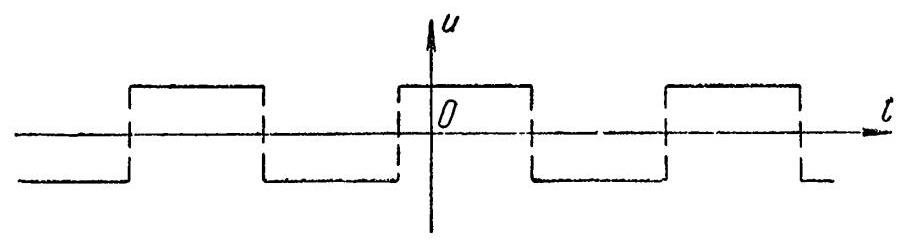
\includegraphics[max width=0.8\textwidth]{images/bo_d547imjef24c73bgfcdg_33_304_1770_905_241_0.jpg}
\end{center}
\hspace*{3em}

Рис. 8.

Для изучения кусков траекторий, соответствующих отрезкам времени, на которых \(u = 1\) и \(u =  - 1\), мы рассмотрим вспомогательную систему

\[
\left. \begin{array}{l} \frac{d{x}^{1}}{dt} = {x}^{2}, \\  \frac{d{x}^{2}}{dt} =  - {x}^{1} \end{array}\right\} \tag{31}
\]

(получающуюся из системы (28) при и = 0). Произвольное решение этой системы может быть записано в виде

\[
{x}^{1} =  - R\cos \left( {t + \gamma }\right) ,\;{x}^{2} = R\sin \left( {t + \gamma }\right) , \tag{32}
\]

где R и γ — постоянные (R ≥ 0,0 ≤ γ < 2π). Таким обра- зом, фазовыми траекториями являются окружности с цент- ром в начале координат:

\[
{\left( {x}^{1}\right) }^{2} + {\left( {x}^{2}\right) }^{2} = {R}^{2} \tag{33}
\]

(рис. 9, a)). Из (32) видно, что движение фазовой точки по окружности (33) совершается по часовой стрелке, при- чем равномерно, с линейной скоростью 2πR (один оборот за время 2π). Отметим, в частности, что за промежуток времени, имеющий длину π, фазовая точка, двигаясь по часовой стрелке, описывает ровно п о л о в и н у окруж- ности (33).

При \(u = 1\) система (28) принимает вид

\[
\left. \begin{array}{l} \frac{d{x}^{1}}{dt} = {x}^{2}, \\  \frac{d{x}^{2}}{dt} =  - {x}^{1} + 1, \end{array}\right\} \tag{34}
\]

или, иначе,

\[
\left. \begin{aligned} \frac{d\left( {{x}^{1} - 1}\right) }{dt} &  = {x}^{2}, \\  \frac{d{x}^{2}}{dt} &  =  - \left( {{x}^{1} - 1}\right) . \end{aligned}\right\} \tag{35}
\]

Вспоминая соотношения (31) и (33), мы находим, что фа- зовые траектории системы (35) (или, что то же самое, системы (34)) представляют собой окружности

\[
{\left( {x}^{1} - 1\right) }^{2} + {\left( {x}^{2}\right) }^{2} = {R}^{2}, \tag{36}
\]

т. е. окружности с центром в точке О1, имеющей коор- динаты (1, 0). Эти окружности фазовая точка, движу- щаяся по закону (34) (т. е. по закону (28) при и = 1), пробегает по часовой стрелке, обходя за время я ровно половину окружности (рис. 9,6).

\begin{center}
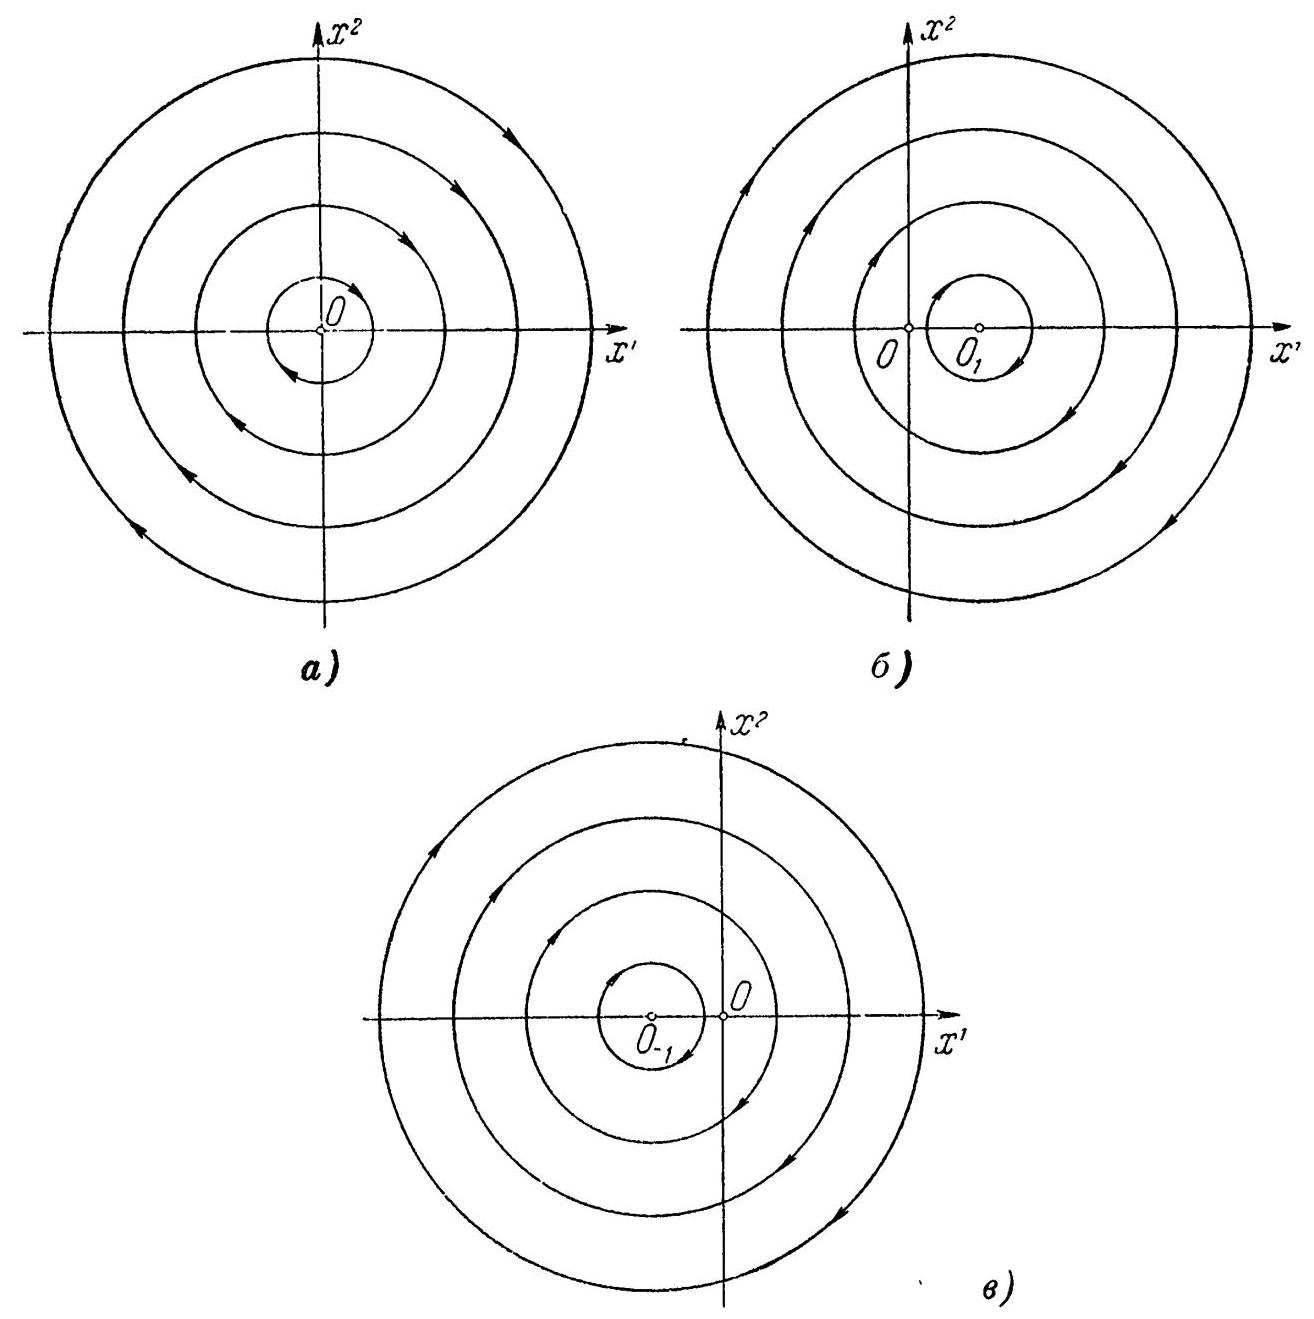
\includegraphics[max width=1.0\textwidth]{images/bo_d547imjef24c73bgfcdg_35_105_395_1314_1319_0.jpg}
\end{center}
\hspace*{3em}

Prac. 9.

Аналогично, при \(u =  - 1\) система (28) принимает вид

\[
\left. \begin{array}{l} \frac{d{x}^{1}}{dt} = {x}^{2}, \\  \frac{d{x}^{2}}{dt} =  - {x}^{1} - 1, \end{array}\right\}
\]

ее фазовыми траекториями являются окружности

\[
{\left( {x}^{1} + 1\right) }^{2} + {\left( {x}^{2}\right) }^{2} = {R}^{2} \tag{37}
\]

c центром в точке 0\_1, имеющей координаты (-1, 0). По этим окружностям фазовая точка движется по часовой стрелке, проходя ровно половину окружности за вре- мя π (рис. 9,6)).

Как было указано выше, каждое оптимальное управ- ление \(u\left( t\right)\) является кусочно-постоянной функцией, полу- чающейся из функции sign (sin t), равной поочередно +1

\begin{center}
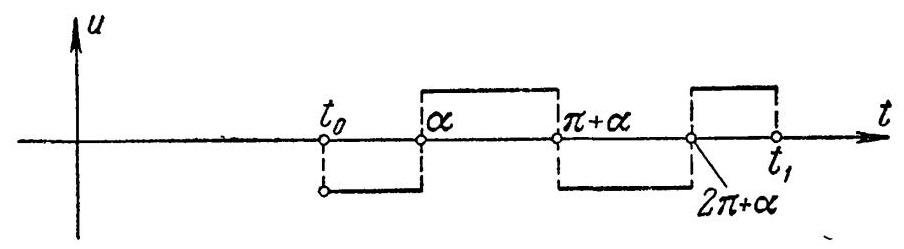
\includegraphics[max width=0.8\textwidth]{images/bo_d547imjef24c73bgfcdg_36_310_754_904_249_0.jpg}
\end{center}
\hspace*{3em}

Pnc. 10.

и —1 на интервалах длины π, при помощи сдвига на некоторый отрезок а, (рис. 8). Если оптимальное управление \(u\left( t\right)\) имеет вид, показанный на рис. 10, т. е. поочередно равно +1 и −1 на интервалах ( и, а), (а, π+-α), \(\left( {\pi  + \alpha,{2\pi } + \alpha }\right),\ldots\) и,в заключе- ние,на некотором интервале дли- ны \(\beta  < \pi\) равно -1, to cootbet- ствующая оптимальная траек- тория может быть построена следующим образом.

\begin{center}
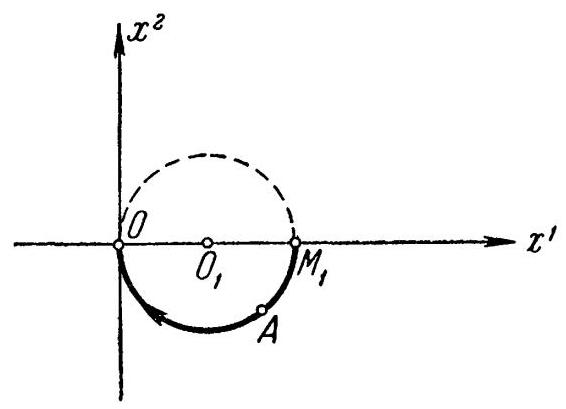
\includegraphics[max width=0.5\textwidth]{images/bo_d547imjef24c73bgfcdg_36_846_1318_566_409_0.jpg}
\end{center}
\hspace*{3em}

Puc. 11a.

В течение заключительного отрезка времени (длины β) фазо- вая точка движется по окруж- ности вида (36) (ибо и = 1 на этом отрезке времени), причем по той из этих окруж- ностей, которая проходит через начало координат (ибо искомая траектория должна вести в начало координат). Такой окружностью является окружность радиуса 1 с цен- тром в точке 0, (рис. 11a). По этой окружности фазо- вая точка попадает в начало координат, проходя ду- ry, меньшую половины окружности ( \textbackslash tô β < π). Таким образом, обозначив нижнюю полуокружность этой окруж- ности через М1О, мы найдем, что заключительный кусок

\begin{center}
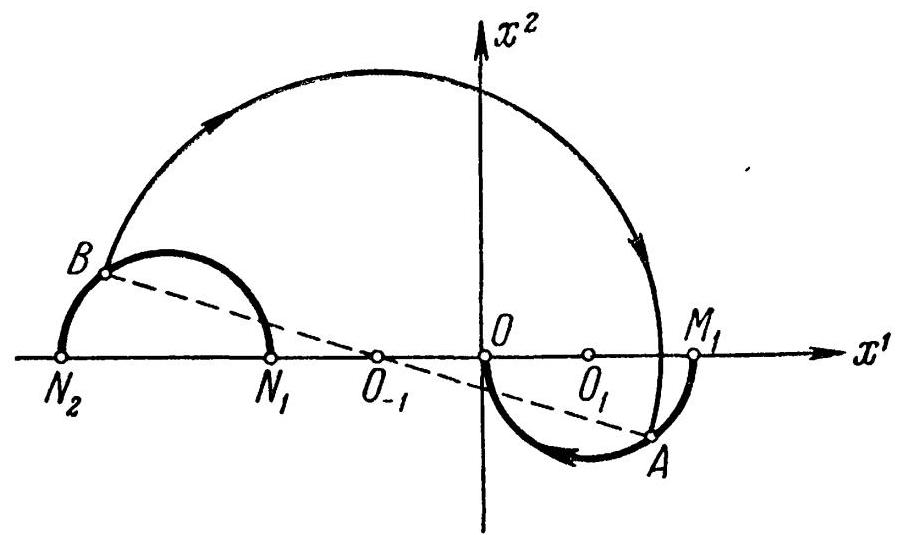
\includegraphics[max width=0.8\textwidth]{images/bo_d547imjef24c73bgfcdg_37_313_314_903_535_0.jpg}
\end{center}
\hspace*{3em}

Pac. 116.

фазовой траектории представляет собой некоторую ду- ry \({AO}\) полуокружности \({M}_{1}O\).

\begin{center}
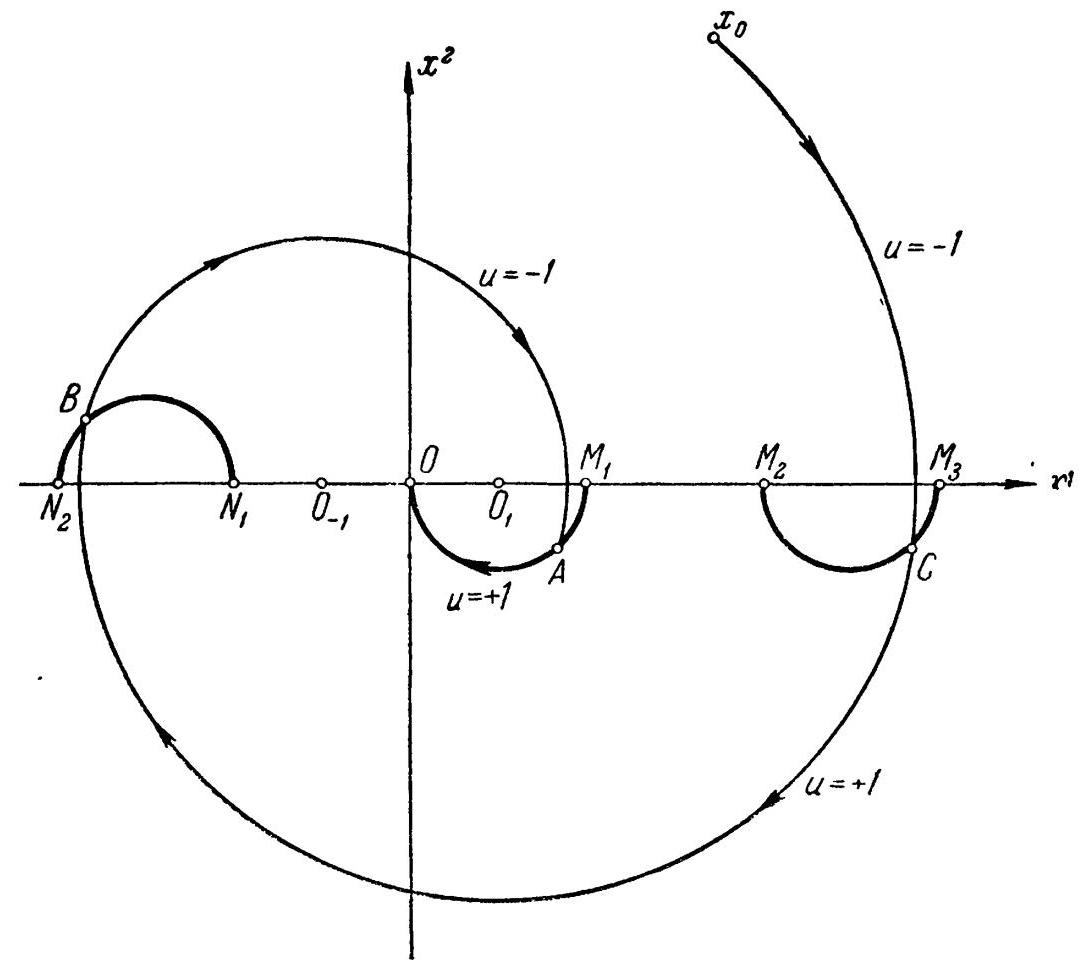
\includegraphics[max width=1.0\textwidth]{images/bo_d547imjef24c73bgfcdg_37_218_1056_1092_961_0.jpg}
\end{center}
\hspace*{3em}

Puc. 11в.

Далее, в положение \(A\) фазовая точка попала, дви- гаясь в течение отрезка времени, имеющего длину π, иол воздействием управления и = — 1 (см. рис. 10), т. е. предыдущий кусок фазовой траектории представляет собой полуокружность \({BA}\) c центром в точке О\_1, кон- чающуюся в точке A (рис. 116). Так как дуга ВА равна полуокружности, то точка В, симметрична А относительно центра О\_1, и потому точка В лежит на полуокружно- сти л, \({\mathrm{N}}_{1}{\mathrm{\;N}}_{2}\), симметричной полуокружности \(O{M}_{1}\) относи- тельпо центра О\_1. Точно так же предшествующая дуге ВА дуга CB, соответствующая отрезку времени длины π, на котором и = 1, равна полуокружности c центром \({O}_{1}\),и потому точка C лежит на полуокружно- сти М2МЗ, которая симметрична полуокружности N1N2 относительно центра О1 (рис. 11в), и т. д. Таким обра- 30M, соответствующая фазовая траектория имеет вид, показанный на рис. 11в (начальный кусок фазовой тра- ектории будет меньше половины окружности, если только \(0 < \alpha  - {t}_{0} < \pi\) ; см. puc. 10).

\begin{center}
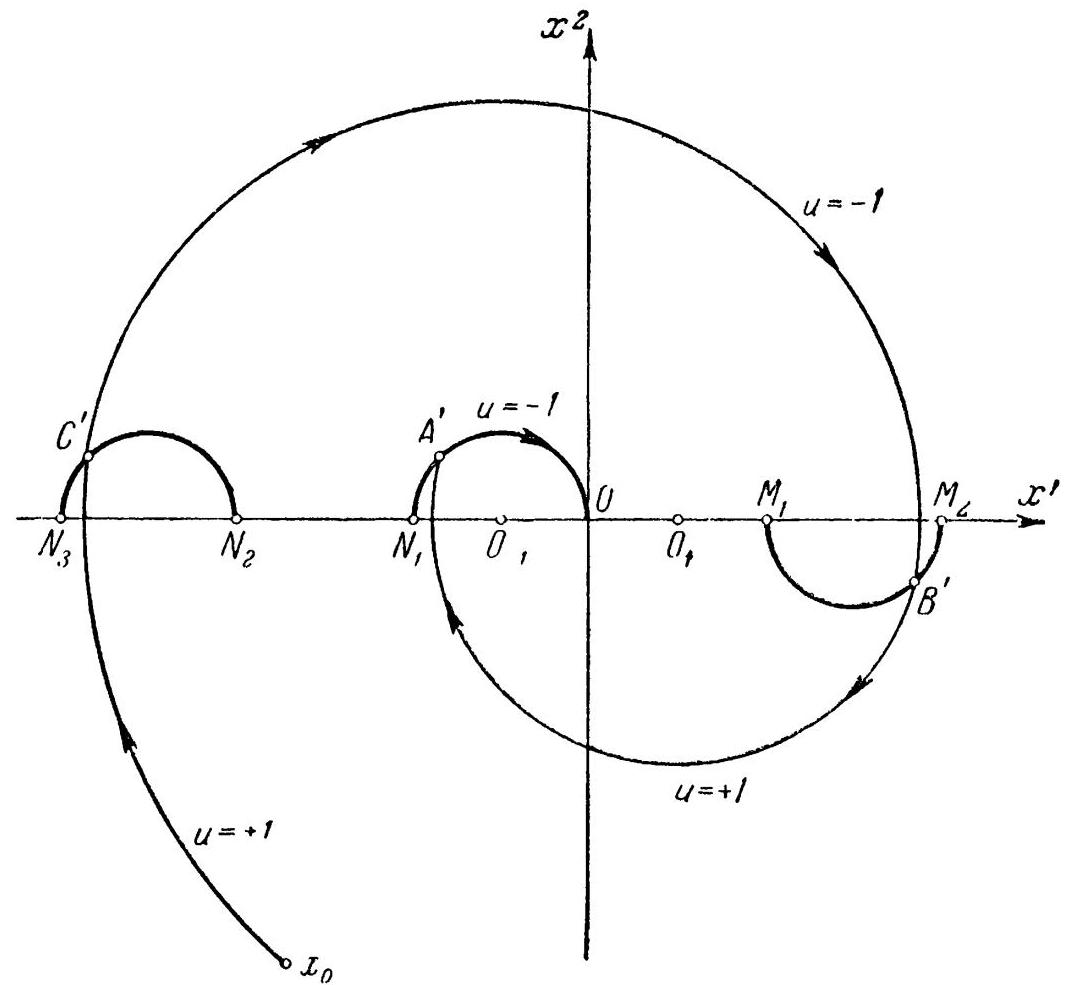
\includegraphics[max width=0.9\textwidth]{images/bo_d547imjef24c73bgfcdg_38_227_653_1073_985_0.jpg}
\end{center}
\hspace*{3em}

Puc. 12.

Фазовая траектория, соответствующая оптималь- ному управлению и (t), которое на заключительном отрезке длины β равно —1 (а не +1), получается из траекто- рии, изображенной на рис. 11в, с помощью цент- ральной симметрии (рис. 12). Для такой траектории точки «стыка» дуг окружностей будут лежать на полу- окружностях \(O{N}_{1}\), \({M}_{1}{M}_{2}\), \({N}_{2}{N}_{3}\), \(\ldots\), cummerputnhux (относительно начала координат) полуокружностям ОМ1, \({N}_{1}{N}_{2},{M}_{2}{M}_{3},\ldots\)

Объединяя оба эти случая (рис. 11в и 12) вместе, получаем всю картину поведения фазовых траекторий (рис. 13). На рис. 13 надписаны на дугах фазовых тра- екторий соответствующие значения управляющего пара- метра и. Из рис. 13 видно, что если начальная точка \({x}_{0}\) расположена в ы ш е линии... \({M}_{3}{M}_{2}{M}_{1}O{N}_{1}{N}_{2}{N}_{3}\ldots\), составленной из бесконечного числа полуокружностей радиуса 1, то фазовая точка должна двигаться под воз- действием управления и = — 1 до тех пор, пока она не попадет на дугу... \({M}_{3}{M}_{2}{M}_{1}O;\) в момент попадания на эту дугу значение и переключается и остается равным +1 (фазовая точка при этом движется н и ж е ли- нии... \({M}_{3}{M}_{2}{M}_{1}O{N}_{1}{N}_{2}{N}_{3}\ldots\) ) до момента попадания на дугу \(O{N}_{1}{N}_{2}{N}_{3}\ldots\) ; затем точка снова движется в ы ш е линии... \({M}_{3}{M}_{2}{M}_{1}O{N}_{1}{N}_{2}{N}_{3}\ldots\) под воздействием управ- ления и е — 1 и т. д. Последний кусок фазовой траектории (ведущий в начало координат) представляет собой дугу полуокружности \({M}_{1}O\) или полуокружно- сти л,0. Совершенно аналогично движется точка и в том случае, если начальная точка хор асположена н и ж е линии... \({M}_{3}{M}_{2}{M}_{1}O{N}_{1}{N}_{2}{N}_{3}\ldots  :\) выше этой линии фа- зовая точка движется под воздействием управления и = = — 1, а ниже этой линии — под воздействием управле- ния \(u =  + 1\).

\begin{center}
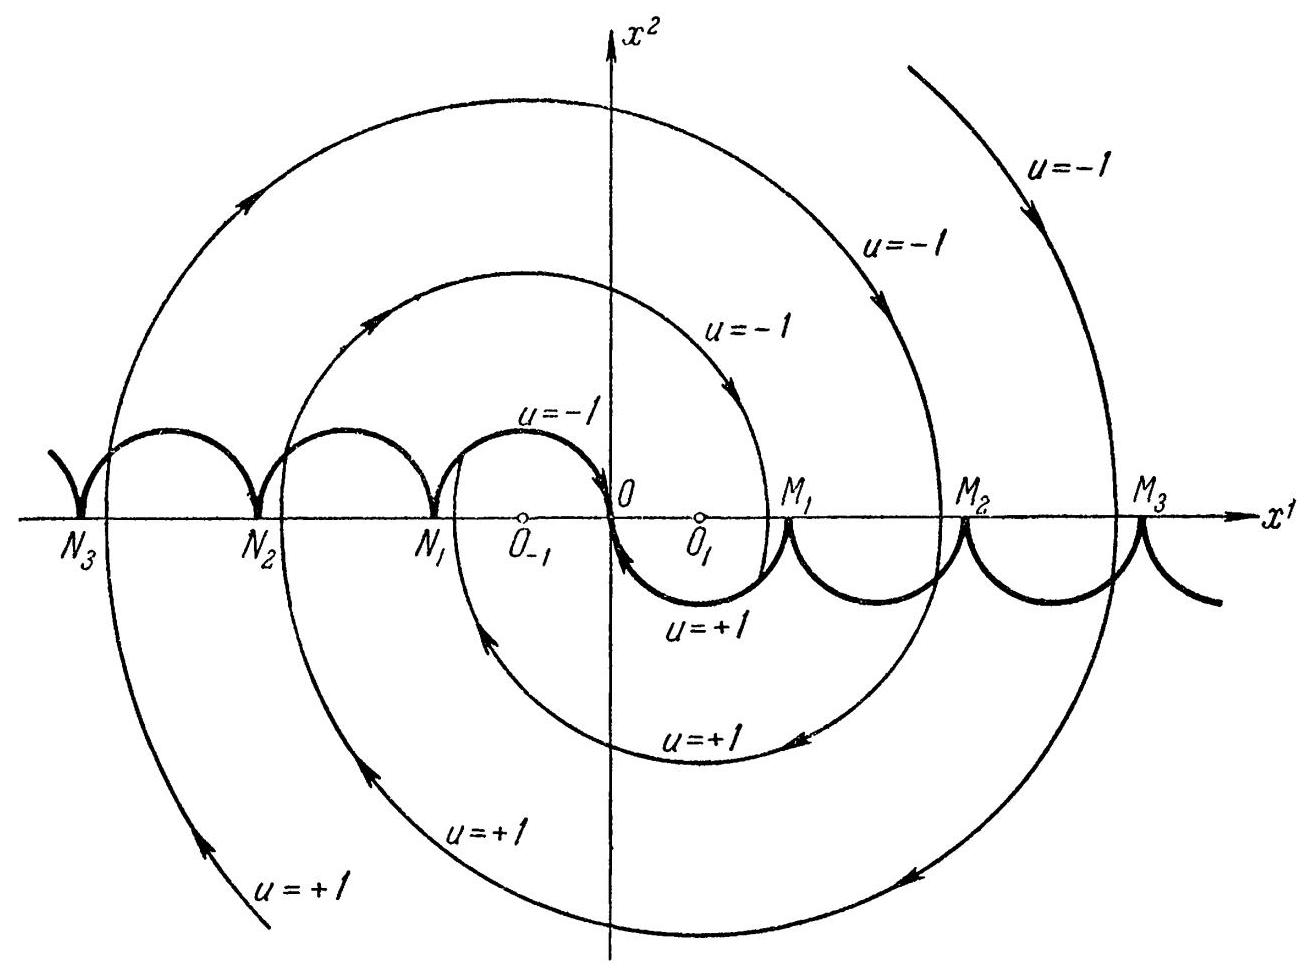
\includegraphics[max width=1.0\textwidth]{images/bo_d547imjef24c73bgfcdg_39_103_668_1311_969_0.jpg}
\end{center}
\hspace*{3em}

Pac. 13.

Итак, согласно теореме 2, только указанные траекто- рии могут быть оптимальными, причем из проведенного исследования видно, что из каждой точки фазовой пло- скости исходит только о д н а траектория, ведущая в нача- ло координат, которая может быть оптимальной. Из тео- ремы существования, доказываемой в главе 3, вытекает, что в рассматриваемом примере для любой начальной точки \({x}_{0}\) существует оптимальная траектория (см. стр. 142). Таким образом, найденные траектории (рис. 13) явля- ются оптимальными, и других оптимальных траекторий, ведущих в начало координат, не существует.

Как и в первом примере, полученное решение опти- мальной задачи можно истолковать следующим образом. Обозначим через v ( \({x}^{1},{x}^{2}\) ) = v (x) функцию, заданную на плоскости \({x}^{1},{x}^{2}\) соотношениями:

\[
v\left( x\right)  =
\begin{cases}
+1, & \text{below the line } \ldots M_{3}M_{2}M_{1}ON_{1}N_{2}N_{3}\ldots \text{ and on the arc } \ldots M_{3}M_{2}M_{1}O; \\
-1, & \text{above the line } \ldots M_{3}M_{2}M_{1}ON_{1}N_{2}N_{3}\ldots .
\end{cases}
\]

Тогда вдоль каждой оптимальной траектории х (t) соот- ветствующее оптимальное управление и (t) имеет вид

\[
u\left( t\right)  = v\left( {x\left( t\right) }\right) .
\]

(28)величину \(u\) функцией \(v\left( x\right)\),мы получим систему

\[
\left. \begin{array}{l} \frac{d{x}^{1}}{dt} = {x}^{2}, \\  \frac{d{x}^{2}}{dt} =  - {x}^{1} + v\left( {{x}^{1},{x}^{2}}\right) , \end{array}\right\} \tag{38}
\]

решение которой (при произвольном начальном состоянии \({x}_{0}\) дает оптимальную фазовую траекторию, ведущую в начало координат. Иначе говоря, система (38) пред- ставляет собой систему дифференциальных уравнений (с разрывной правой частью) для нахождения оптималь- ных траекторий, ведущих в начало координат.

\(\Pi\) p \(u\) м е р 3

Рассмотрим теперь систему с двумя управляющими параметрами:

\[
\left. \begin{array}{l} \frac{d{x}^{1}}{dt} = {x}^{2} + {u}^{1}, \\  \frac{d{x}^{2}}{dt} =  - {x}^{1} + {u}^{2}, \end{array}\right\} \tag{39}
\]

причем величины и, и а подчиним условиям и и \(\left| {u}^{2}\right|  \leq  1\). Для этой системы мы, как и в двух первых примерах, изучим задачу о быстрейшем попадании в начало координат. Выпишем функцию H

\[
H = {\psi }_{1}\left( {{x}^{2} + {u}^{1}}\right)  + {\psi }_{2}\left( {-{x}^{1} + {u}^{2}}\right) \tag{40}
\]

и вспомогательную систему

\[
\left. \begin{array}{l} \frac{d{\psi }_{1}}{dt} = {\psi }_{2}, \\  \frac{d{\psi }_{2}}{dt} =  - {\psi }_{1}. \end{array}\right\}
\]

Из этой системы мы получаем

\[
{\psi }_{1} = A\sin \left( {t + \alpha }\right)
\]

\[
{\psi }_{2} = A\cos \left( {t + \alpha }\right)
\]

где \(A\) и \(\alpha  -\) постоянные; \(A > 0,0 \leq  \alpha  < {2\pi }\). Соотнопение (20) дает нам теперь (учитывая (40) и условия |и'|≤1, \(\left| {u}^{2}\right|  \leq  1)\)

(41)
\[
{u}^{1} = \operatorname{sign}{\psi }_{1} = \operatorname{sign}\left( {A\sin \left( {t + \alpha }\right) }\right)  = \operatorname{sign}\left( {\sin \left( {t + \alpha }\right) }\right) ,
\]

\[
{u}^{2} = \operatorname{sign}{\psi }_{2} = \operatorname{sign}\left( {A\cos \left( {t + \alpha }\right) }\right)  = \operatorname{sign}\left( {\cos \left( {t + \alpha }\right) }\right) .
\]

Таким образом, в случае оптимального управления каж- дый из управляющих параметров и", и г является кусочно- постоянной функцией, принимающей значения +1 и -1. Из рассмотрения системы (39) мы легко заключаем, что куски фазовых траекторий, соответствующие отрезкам вре- мени, на которых и 41 е 1, и редставляют собой дуги окружностей с центром в точке 0,1, имеющей коорди- наты (1,—1). Аналогично при и" 1, и" = -1 и т. д., как это указано в следующей таблице:

\begin{center}
\adjustbox{max width=\textwidth}{
\begin{tabular}{|c|c|}
\hline
Постоянные значения управляющих параметров на некотором отрезке вре. мени & Центр окружностей, являющихся соответствующими фазовыми траекториями системы (39) \\
\cline{1-2}
\makecell{ \({u}^{1} = 1,\;{u}^{2} = 1\) \\ \({u}^{1} =  - 1,{u}^{2} = 1\) \\ \({u}^{1} =  - 1,{u}^{2} =  - 1\) \\ \({u}^{1} = 1,\;{u}^{2} =  - 1\) } & \makecell{ \({O}_{1,1}\) с координатами (1,—1) \\ \({O}_{-1,1}\) с координатами (1, 1) \\ Точка \({O}_{-1, - 1}\) с координатами (— \\ Точка \({O}_{1, - 1}\) c коордпнатами (—1,—1) } \\
\cline{1-2}
\hline
\end{tabular}
}
\end{center}

Во всех случаях движение по соответствующим фазо- вым траекториям (окружностям) совершается по часовой стрелке, причем равномерно, со скоростью один оборот за время 2π. В частности, за время, равное д т фазовая точка пробегает чет в ерть о кружности.

Из (41) следует, что в тот момент, когда аргумент \(t + \alpha\) проходит через точки \(k\frac{\pi }{2}\;(k -\) произвольное це- лое число), один из управляющих параметров и", и2 меняет знак (так как в каждой из этих точек либо си- нус, либо косинус проходит через нуль). Иначе говоря, в моменты времени, для которых \(t + \alpha  = k\frac{\pi }{2}\), происхо- дит смена значений управляющих параметров и’, и’, т. е. происходит с м е н а п е н т р а окружности, по которой движется фазовая точка. Такая смена центра происходит через каждые 2 ещиниц времени, так что фазовая тра- ектория составлена из четвертей окружностей с цент- рами \({O}_{1.1};{O}_{-{1.1}};{O}_{-1, - 1};{O}_{{1.1} - 1}\). Исключение составляют только первый и последний куски фазовой траектории:

Далее, нетрудно понять, в каком порядке происходит смена центров. Если при возрастании \(t\) аргумент \(t + \alpha\) проходит через значение \(t + \alpha  = {2k\pi }\left( {k - \text{ целое число), }}\right)\) то непосредственно π e p e д этим моментом выполнялись COOTHOMEHIH \({u}^{1} =  - 1,{u}^{2} =\) = + 1 (см. (41)), т. е. дви- жение происходило по дуге c центром \({O}_{-{1.1}}\), a п о с л е они могут оказаться меньши- ми, чем четверть окружности. этого момента выполняются соотношения \({u}^{1} =  + 1,{u}^{2} =  + 1\), т. е. движение происходит по дуге с центром \({O}_{1,1}\). Иначе говоря, центр \({O}_{-1,1}\) сменяется центром \({O}_{1,1}\). Аналогично, центр \({O}_{1,1}\) сменяется центром \({O}_{1, - 1}\) (при прохождении ар-гумента \(t + \alpha\) через значение \({2k\pi } + \frac{\pi }{2}\) (см. (41)),центр \({O}_{1, - 1} \; {c}_{M\text{ еняется центром }}{O}_{-1, - 1}\), a центр \({O}_{-1, - 1}\) - центром \({O}_{-1,1}\). На рис. 14 стрелки указывают порядок смены центров.

\begin{center}
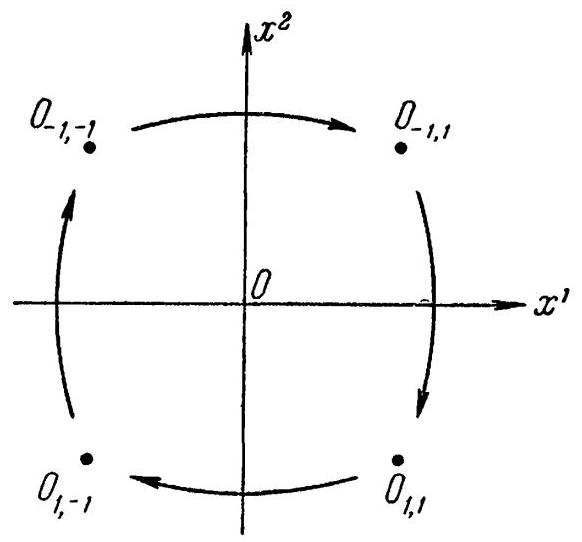
\includegraphics[max width=0.5\textwidth]{images/bo_d547imjef24c73bgfcdg_43_129_476_582_542_0.jpg}
\end{center}
\hspace*{3em}

Pnc. 14.

Теперь уже нетрудно представить себе поведение фазовых траекторий. Для этого мы проведем следующее вспомогательное построение. Рассмотрим окружность с центром \({O}_{-1,1}\),проходящую через начало координат, и обозначим через ОМ дугу этой окружности, располо- женную под осью абсцисс (дуга ОМц равна, очевидно, четверти окружности). Далее, обозначим через \({M}_{1}{M}_{2}\) дугу, равную ОМ и получающуюся из нее переносом на отрезок ОМ1; аналогично построим дугу М2, и т. д. (рис. 15). Заметим, что абсциссы точек М1, М2, \({M}_{3}\ldots\) равны соответственно \(2,4,6,\ldots \Pi\) овернув теперь линию \(O{M}_{1}{M}_{2}{M}_{3}\ldots\), составленную из равных чет- вертей окружностей, на углы 2 л, я 2 м из вокруг начала координат, мы получим изображенные на рис. 16 линии \(O{N}_{1}{N}_{2}{N}_{3}\ldots,O{P}_{1}{P}_{2}{P}_{3}\ldots,O{Q}_{1}{Q}_{2}{Q}_{3}\ldots\)

\begin{center}
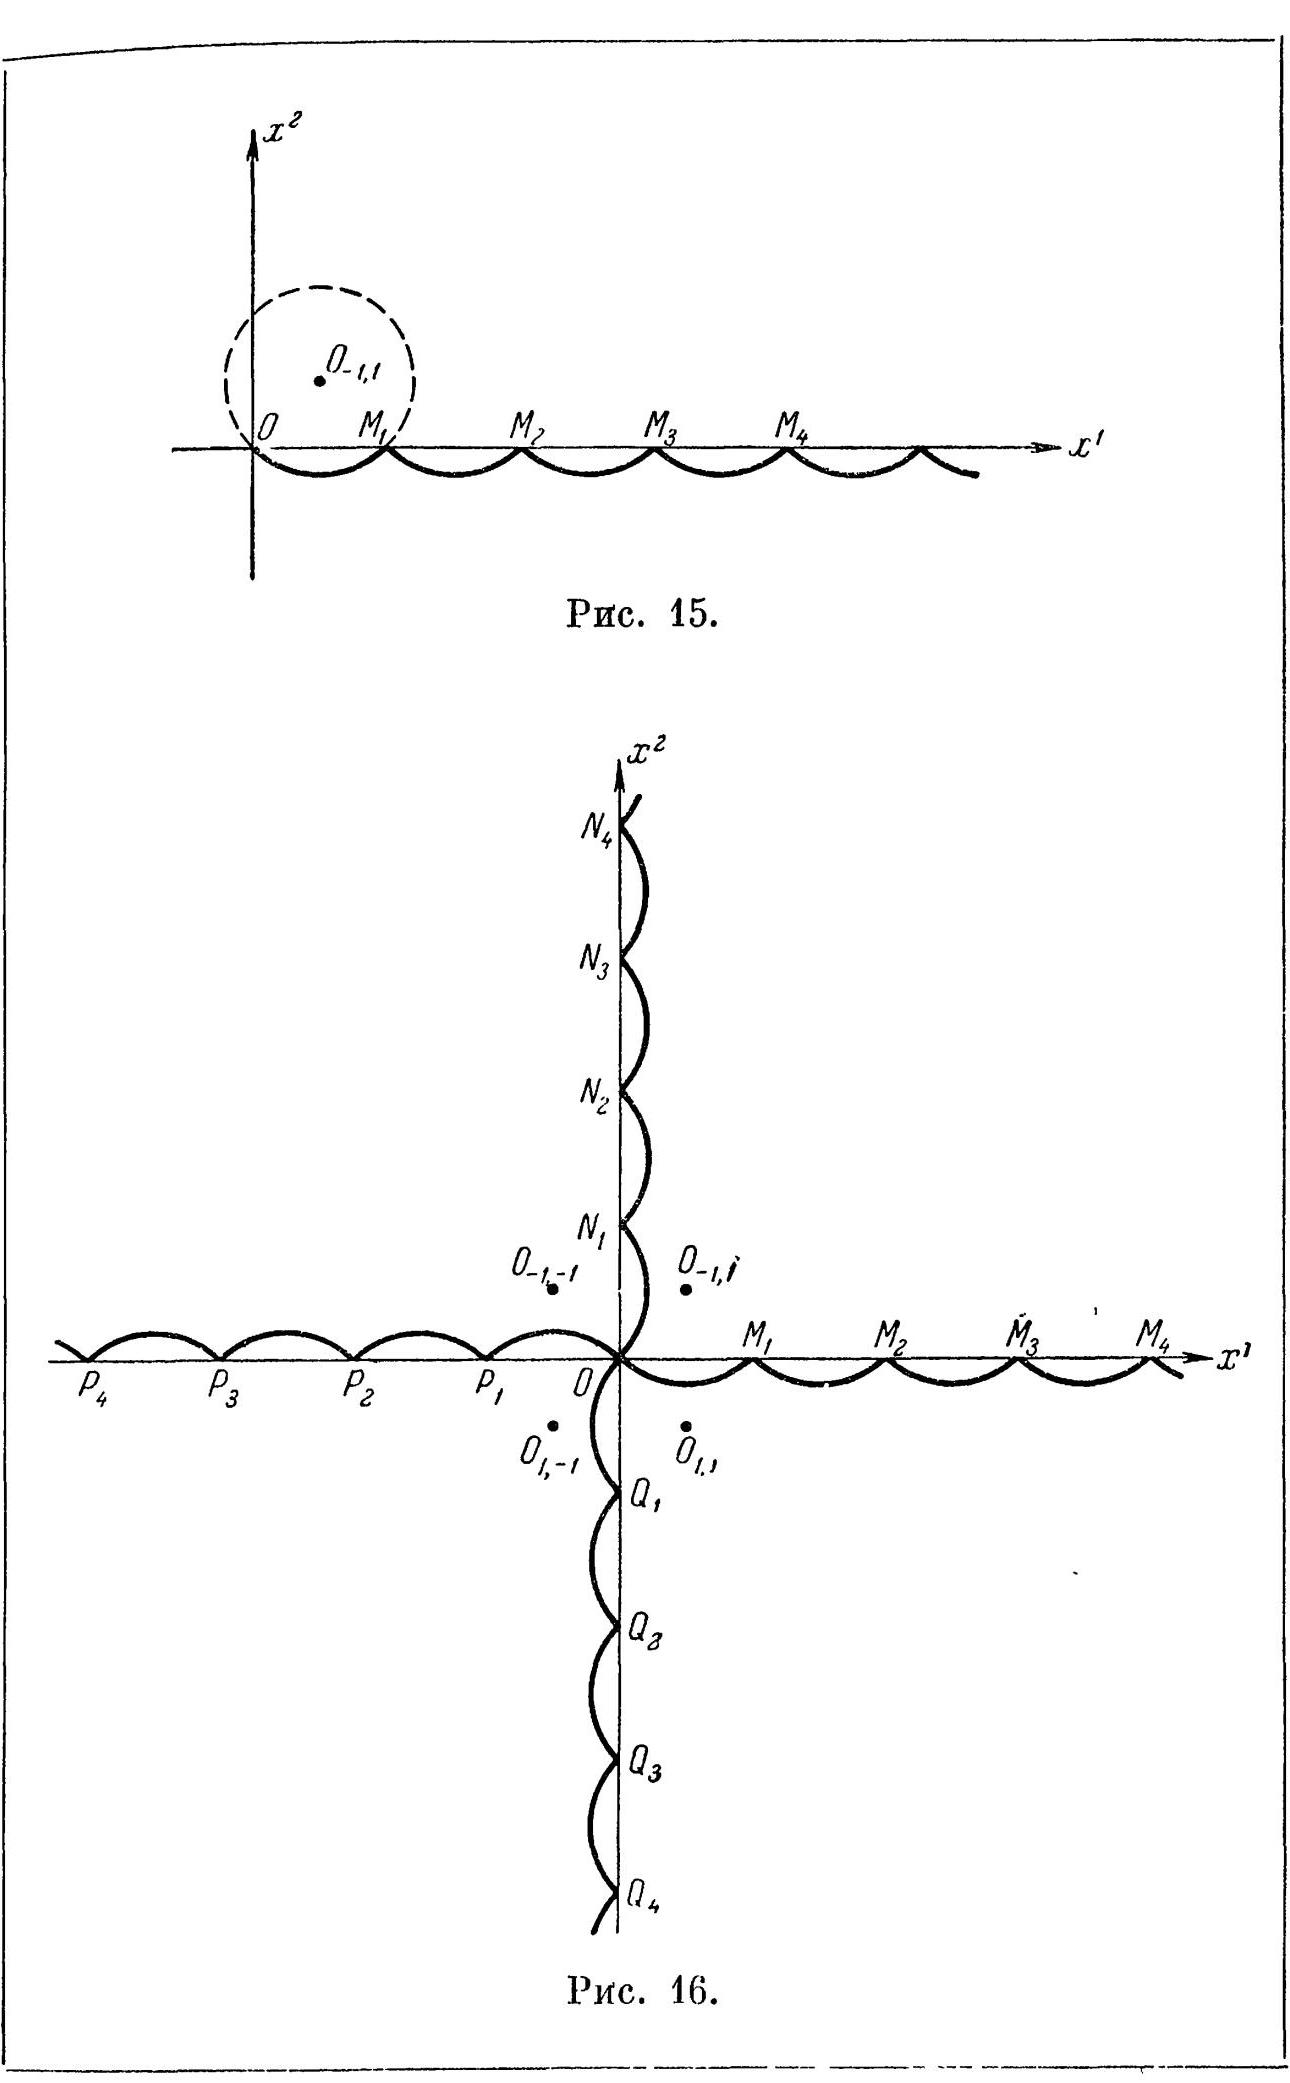
\includegraphics[max width=1.0\textwidth]{images/bo_d547imjef24c73bgfcdg_44_133_240_1290_2083_0.jpg}
\end{center}
\hspace*{3em}

Теперь начнем строить фазовую траекторию. Возьмем оптимальное управление (имеющее на некотором конечном отрезке времени вид (41)) и предположим для определен- ности, что на п о с л е д н е м участке постоянства, имею- щем длину \(\beta  < \frac{\pi }{2}\), управляющие параметры принимают значения \({u}^{1} =  + 1,{u}^{2} =  + 1\). Соответствующий кусок фазо- вой траектории (рис. 17, а) представляет собой некоторую дугу АО четверти окружности \({Q}_{1}O\) (ибо этот кусок лежит на окружности с центром 0,1, и оканчивается в начале координат, а длина этого куска не превосходит четверти окружности). Согласно сказанному выше, центру О.1 предшествует центр \({O}_{-1,1}\) (puc. 14), \(\mathbf{n}\) потому участок фазовой траектории, предшествующий точке A, является четвертью окружности с центром 0\_1.1 (дуга BA на рис. 17, б)). Управляющие параметры имеют на этом участке значения \({u}^{1} =  - 1,{u}^{2} =  + 1\). Так как точка А находилась на дуге \({Q}_{1}O\), то точка В будет находиться на дуге, получающейся из \({Q}_{1}O\) поворотом на угол \(\frac{\pi }{2}\) вокруг точки \({O}_{-1,1}\),т. e. на дуге \({M}_{1}{M}_{2}\).

Далее, центру О-ди, предшествует центр О-д-1, и потому кусок фазовой траектории, предшествующий точке В, представлял собой четверть окружностя с центром в точке О\_1.— (дуга CB на рис. 17, е)). Управ- ляющие параметры имеют значения и" = — 1, и* 2 = — 1. Tak как точка B находилась на дуге \({M}_{1}{M}_{2}\), то точка C будет находиться на дуге, получающейся из \({M}_{1}{M}_{2}\) поворотом на угол 2 вокруг точки \({O}_{-1, - 1}\), т. е. на дуге \({N}_{2}{N}_{3}\). Продолжая таким образом, можно вычертить всю фазовую траекторию. На рис. 17, e) пока- зана фазовая траектория, составленная из трех дуг, яв- ляющихся четвертями окружностей, и двух дуг (на- чальной и конечной), каждая из которых меньше чет- верти окружности.

Если бы мы предположили, что на последнем уча- стке постоянства управляющие параметры принимают не значения \({u}^{1} =  - 1,{u}^{2} =  + 1\), a значения \({u}^{1} =  - 1,{u}^{2} =  + 1\) или значения \({u}^{1} =  - 1,{u}^{2} =  - 1\) или,наконец,значения \({u}^{1} =  + 1,{u}^{2} =  - 1\), то построили бы аналогичные фазовые

\begin{center}
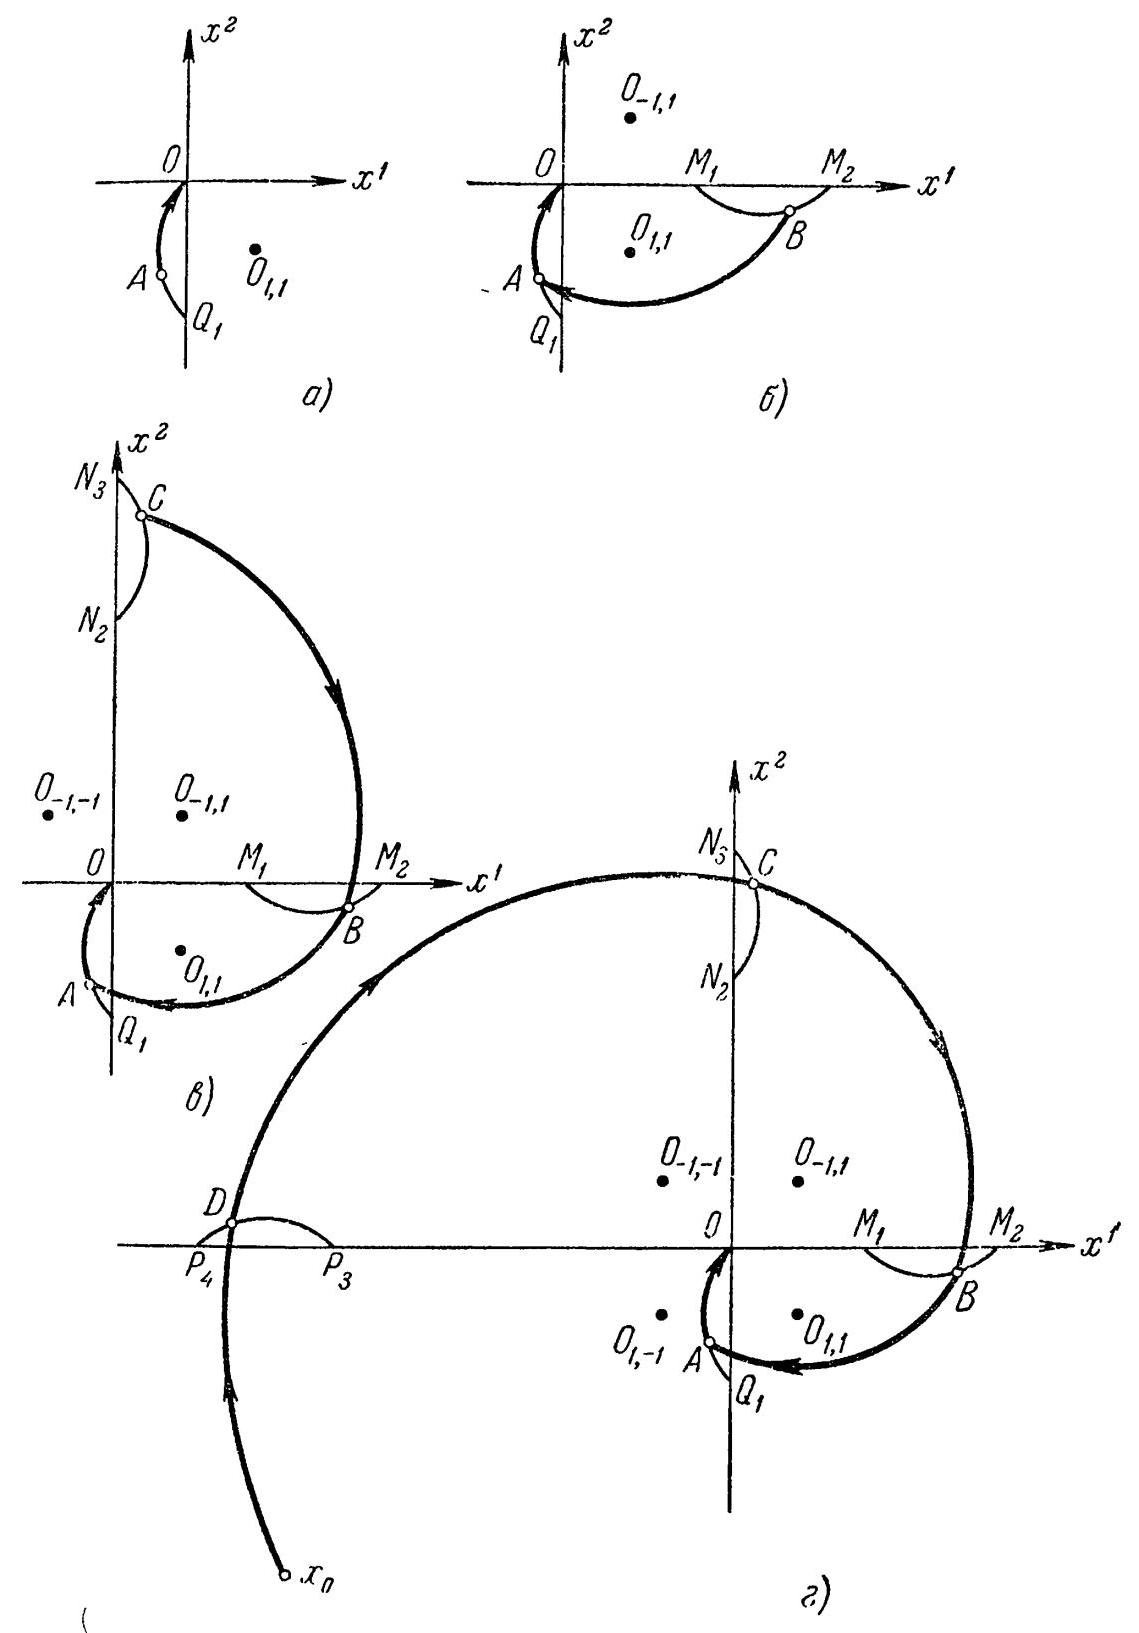
\includegraphics[max width=1.0\textwidth]{images/bo_d547imjef24c73bgfcdg_46_193_336_1139_1633_0.jpg}
\end{center}
\hspace*{3em}

Pnc. 17.

траектории, получающиеся из траектории, изображен- ной на рис. 17, е), поворотом на углы д я, я, 3. Четыре получающиеся таким образом фазовые траектории изобра- жены на рис. 18.

Анализируя значения управляющих параметров на отдельных кусках всех получающихся таким образом фазовых траекторий, мы приходим к следующему выво- ду. Линии \(O{M}_{1}{M}_{2}{M}_{3}\ldots,O{N}_{1}{N}_{2}{N}_{3}\ldots,O{P}_{1}{P}_{2}{P}_{3}\ldots\), \(O{Q}_{1}{Q}_{2}{Q}_{3}\ldots\) разбивают плоскость на четыре части, четы- ре «криволинейных квадранта», которые мы обозначим римскими цифрами I, II, III, IV (рис. 19). На кусках фазовых траекторий, расположенных в «квадранте» I, управляющие параметры принимают значения и" == 1, \({u}^{2} =  - 1\). Под действием этого управления фазовая точка достигает линии \(O{M}_{1}{M}_{2}{M}_{3}\ldots\),и в момент попадания на эту линию значения управляющих параметров пере- ключаются и становятся равными и" == 1, и 2 == + 1. Под действием этого управления фазовая точка движется

\begin{center}
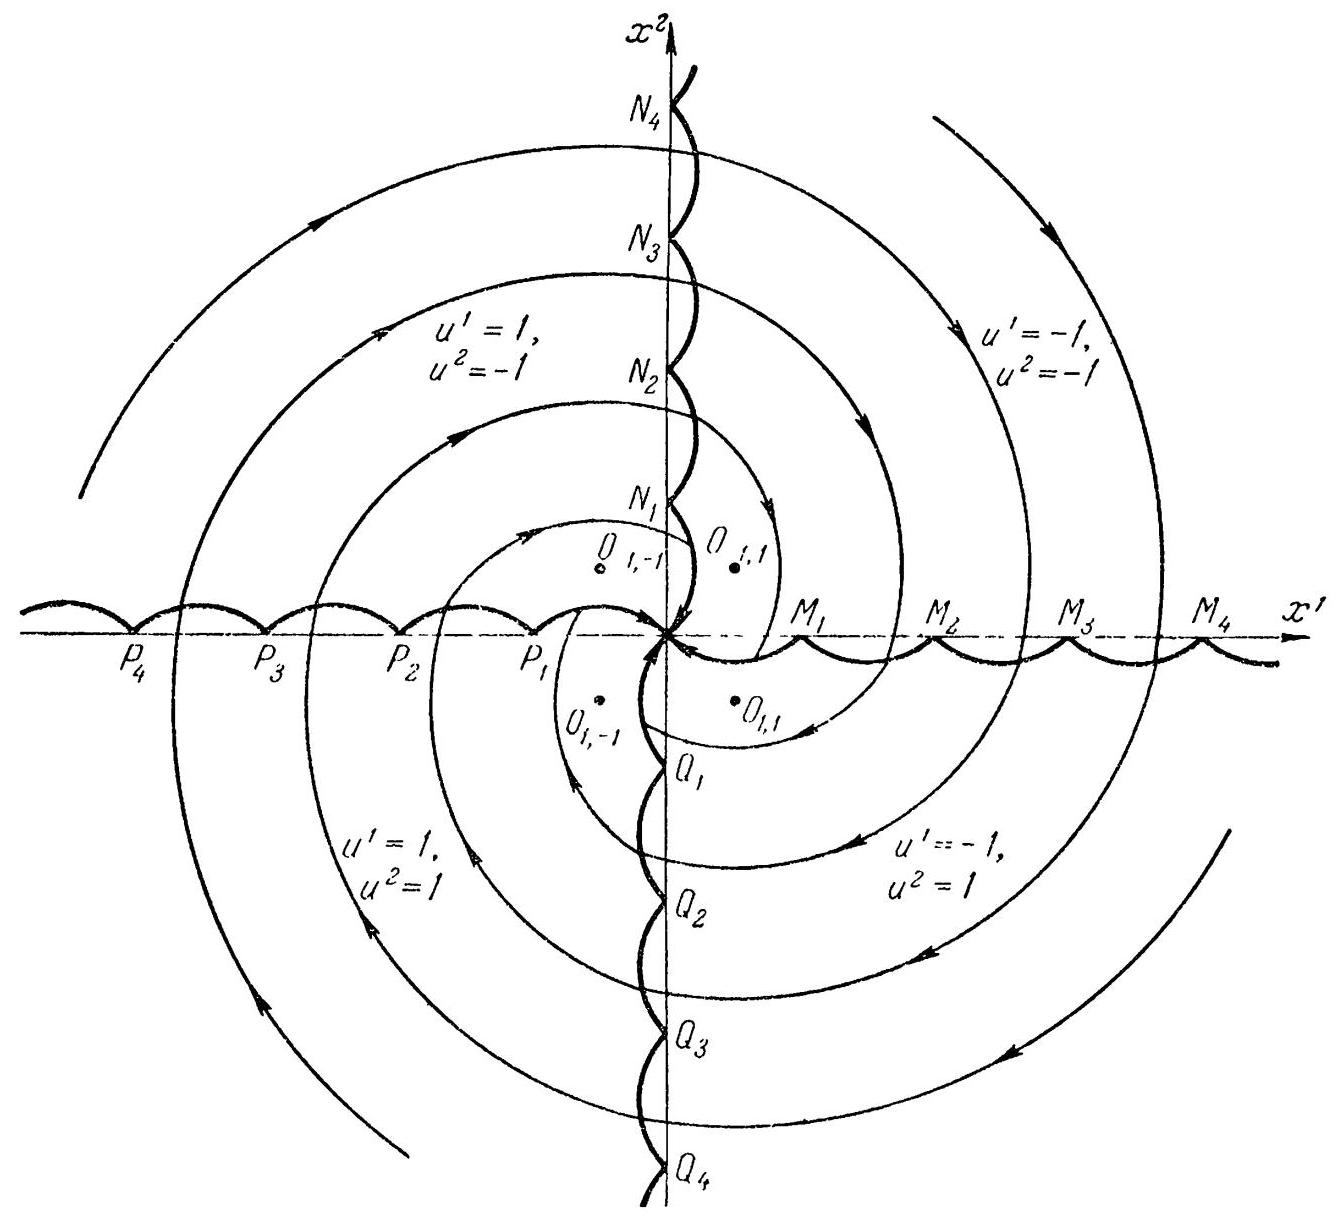
\includegraphics[max width=1.0\textwidth]{images/bo_d547imjef24c73bgfcdg_47_85_433_1340_1215_0.jpg}
\end{center}
\hspace*{3em}

Prac. 18.

\begin{center}
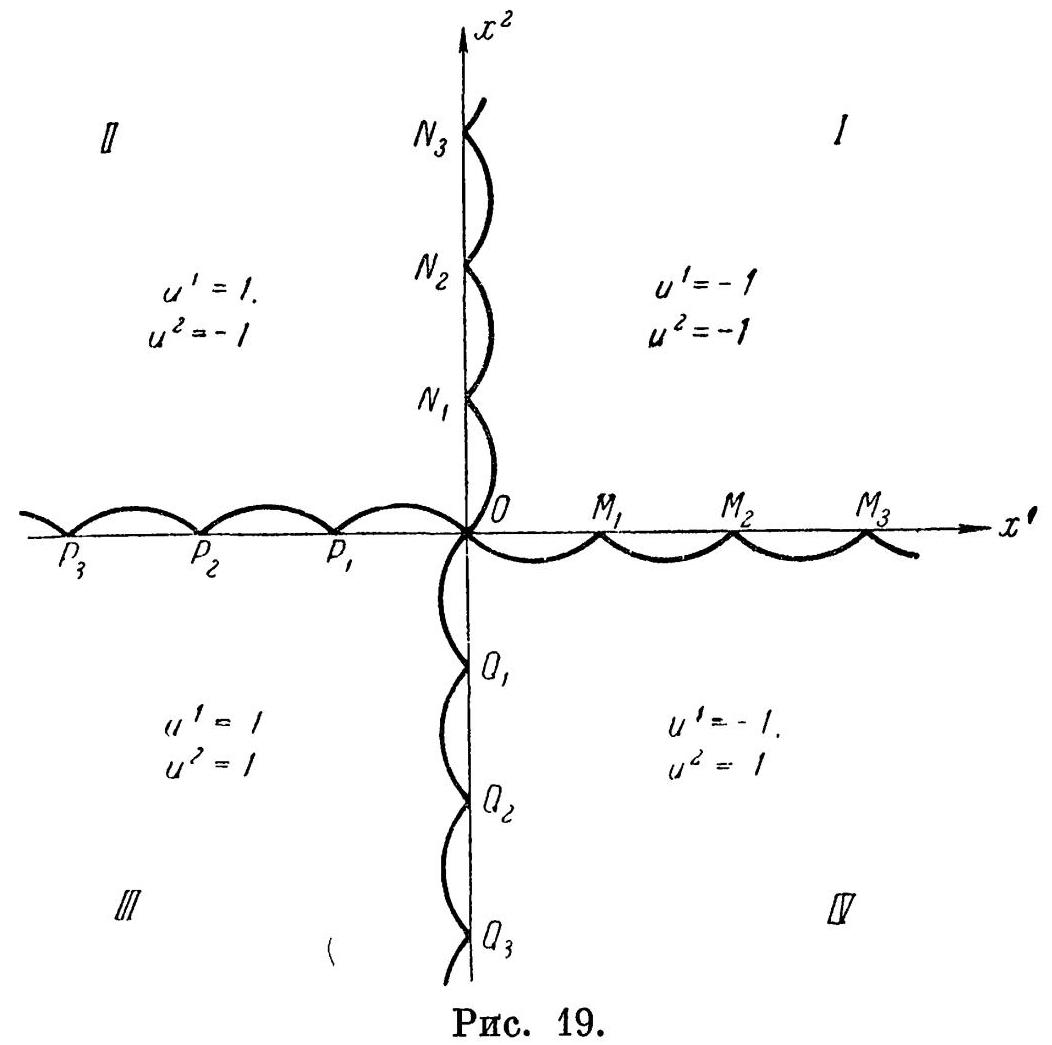
\includegraphics[max width=0.9\textwidth]{images/bo_d547imjef24c73bgfcdg_48_237_374_1052_1045_0.jpg}
\end{center}
\hspace*{3em}

в «квадранте» IV и достигает линии ООЦО,Води..., при- чем в момент попадания на эту линию управляющие параметры принимают значения \({u}^{1} =  + 1,{u}^{2} =  + 1\) и т. д. Все эти факты собраны в следующей таблице:

\begin{center}
\adjustbox{max width=\textwidth}{
\begin{tabular}{|c|c|}
\hline
в «квадранте» & \({u}^{1} =  - 1,{u}^{2} =  - 1\) \\
\cline{1-2}
\(O{P}_{1}{P}_{2}\cdots\) & \({u}^{1} =  + 1,{u}^{2} =  - 1\) \\
\cline{1-2}
в «квадранте» дранте» III и на линии ООдо... & \({u}^{1} =  + 1,{u}^{2} =  + 1\) \\
\cline{1-2}
\({\mathit{{OM}}}_{1}{M}_{2}\cdots\) & \({u}^{1} =  - 1,{u}^{2} =  + 1\) \\
\cline{1-2}
\hline
\end{tabular}
}
\end{center}

Итак, согласно теореме 2, только найденные траекто- рии могут быть оптимальными, причем из проведенного исследования видно, что из каждой точки фазовой пло- скости исходит только о д н а траектория, ведущая в начало координат, которая может быть оптимальной. Из теоремы существования (гл. 3) вытекает, что в рассматриваемом примере для любой начальной точки \({x}_{0}\) существует оптимальная траектория (см. стр. 142). Таким образом, найденные траектории (рис. 18) являются опти- мальными, и других оптимальных траекторий, ведущих в начало координат, не существует.

Как и в двух первых примерах, полученное решение оптимальной задачи можно истолковать следующим обра- зом. Построим на плоскости \({x}^{1},{x}^{2}\) две функции \({v}^{1}\left( {{x}^{1},{x}^{2}}\right)\) и \({v}^{2}\left( {{x}^{1},{x}^{2}}\right)\) :

\[
{v}^{1}\left( {{x}^{1},{x}^{2}}\right)  = \begin{cases}  + 1 & \text{ пвеве линий }\ldots {Q}_{3}{Q}_{2}{Q}_{1}O{N}_{1}{N}_{2}{N}_{3}\ldots \\ & \text{ пв на дуте }\ldots {Q}_{3}{Q}_{2}{Q}_{1}O, \\   - 1 & \text{ правее линии }\ldots {Q}_{3}{Q}_{2}{Q}_{1}O{N}_{1}{N}_{2}{N}_{3}\ldots \\ & \text{ пвиадуте }\ldots {N}_{3}{N}_{2}{N}_{1}O; \end{cases}
\]

\[
{v}^{2}\left( {{x}^{1},{x}^{2}}\right)  = \begin{cases}  + 1 & \text{ ниже линии } \ldots {P}_{3}{P}_{2}{P}_{1}O{M}_{1}{M}_{2}{M}_{3}\ldots \\ & \text{ пния путе } \ldots {M}_{3}{M}_{2}{M}_{1}O, \\   - 1 & \text{ выппе линийи } \ldots {P}_{3}{P}_{2}{P}_{1}O{M}_{1}{M}_{2}{M}_{3}\ldots \\ & \text{ плнаддуте } \ldots {P}_{3}{P}_{2}{P}_{1}O. \end{cases}
\]

Тогда вдюль каждой оптимальной траектории \(x\left( t\right)  = \; = \left( {{x}^{1}\left( t\right),{x}^{2}\left( t\right) }\right)\) соответствующее оптимальное управление \(u\left( t\right)  = \left( {{u}^{1}\left( t\right),{u}^{2}\left( t\right) }\right)\) имеет вид

\[
{u}^{1}\left( t\right)  = {v}^{1}\left( {{x}^{1}\left( t\right) ,{x}^{2}\left( t\right) }\right) ,\;{u}^{2}\left( t\right)  = {v}^{2}\left( {{x}^{1}\left( t\right) ,{x}^{2}\left( t\right) }\right) .
\]

Это означает, что, заменив в системе (39) величины \({u}^{1}\), \({u}^{2}\phi\) ункциями \({v}^{1}\left( {{x}^{1},{x}^{2}}\right),{v}^{2}\left( {{x}^{1},{x}^{2}}\right)\),мы получим систему

\[
\left. \begin{array}{l} \frac{d{x}^{1}}{dt} = {x}^{2} + {v}^{1}\left( {{x}^{1},{x}^{2}}\right) , \\  \frac{d{x}^{2}}{dt} =  - {x}^{1} + {v}^{2}\left( {{x}^{1},{x}^{2}}\right) , \end{array}\right\} \tag{42}
\]

решение которой (при произвольном начальном состоя- нии \({x}_{0}\) ) дает оптимальную фазовую траекторию, ведущую в начало координат. Иначе говоря, система (42) пред- ставляет собой систему дифференциальных уравнений (с разрывными правыми частями) для нахождения опти- мальных траекторий, ведущих в начало координат. Задача синтеза оптимальных управлений

Рассмотренные выше примеры показывают, что реше- ние задачи об оптимальных управлениях естественно ожидать в следующей форме. Будем решать оптималь- ную задачу в общей постановке (см. (9)), рассматривая всевозможные начальные состояния \({x}_{0}\) и каждый раз предписывая в качестве конечного состояния начало координат 0 пространства X. Тогда (насколько можно судить по разобранным выше примерам) существует такая функция v (x), заданная в фазовом пространстве X и принимающая значения в области управления U, что уравнение

\[
\frac{dx}{dt} = f\left( {x,v\left( x\right) }\right) \tag{43}
\]

(cp. (5)) определяет все оптимальные траектории, веду- щие в начало координат. Иначе говоря, оптимальное управление оказывается естественным искать не в форме \(u = u\left( t\right)\), a в форме \(u = v\left( x\right)\),т. e. искомое оптимальное управление в каждый момент зависит лишь от того, в какой точке пространства находится в данный момент фазовая точка. Это и понятно: ведь если мы уже попали в фазовую точку х, то и дальнейшее движение (из точки х в О) должно быть оптимальным (ибо часть оптимальной траектории сама является оптимальной траекторией, см. стр. 22). Поэтому значение оптимального управле- ния \(u\left( t\right)\) в момент прохождения фазовой точкой положе- ния \(x\) зависит только от \(x\), a не от того, в какой точке начиналось движение и сколько времени фазовая точка уже двигалась, прежде чем попала в положение х. Фор- мулы (27), (38), (42) как раз и дают решение разбирав- шихся оптимальных задач в форме дифференциального уравнения (43) с разрывной правой частью. (Если область управления U является множеством r-мерного пространства переменных \({u}^{1},\;{u}^{2},\ldots,{u}^{r}\),то задание одной векторной функции \(v\left( x\right)\) равносильно заданию r скалярных функций \({u}^{1} = {v}^{1}\left( x\right),\ldots,{u}^{r} = {v}^{r}\left( x\right)\) ; cp. фор- мулы (42).)

Функцию \(v\left( x\right)\),дающую уравнение оптимальных траек- торий в форме (43), мы будем называть синтезирующей функцией, а задачу нахождения синтезирующей функции (если таковая существует хотя бы в достаточно малой окрестности начала координат) будем называть задачей синтеза оптимальных управлений. В разобранных выше примерах синтезирующие функции были кусочно- непрерывными.

Знание синтезирующей функции позволяет считать задачу оптимального попадания в начало координат м а т е м а т и ч е с к и решенной до конца. В самом деле, если рассматриваемый технический объект будет снаб- жен измерительным прибором, замеряющим фазовые состояния, и исполнительным механизмом, ставящим рули в положение \(u = v\left( x\right)\),где \(v\left( x\right)\) — синтезирующая функ- ция (предполагаемая известной), то интересующий нас объект будет двигаться оптимально. Если функция \(v\left( x\right)\) имеет сложный вид, то для нахождения нужного поло- жения рулей и = v (x), по-видимому, целесообразно при- менять (универсальные или специализированные) быстро- действующие вычислительные устройства. Читателя, интересующегося этим вопросом, мы отсылаем к обшир- ной монографии А. А. Фельдбаума «Вычислительные устройства в автоматических системах», Физматгиз, Москва, 1959 (см. гл. XIII).

В общем случае задача синтеза (т. е. вопрос о суще- ствовании синтезирующей функции и ее отыскании) не решена. В частном случае линейных систем и опти- мальности, понимаемой в смысле быстродействия, эта задача будет обсуждаться ниже в третьей главе.

\section*{§ 6. Задача с подвижными концами и условия трансверсальности}

Для формулировки и решения дальнейших задач об отыскании оптимальных управлений нам будут необходимы некоторые геометрические понятия. Для удобства чита- теля мы напомним здесь определения этих понятий.

Пусть \(f\left( x\right)  = f\left( {{x}^{1},{x}^{2},\ldots,{x}^{n}}\right)\) — некоторая действитель- ная скалярная функция, заданная в какой-либо обла- сти G евклидова *) пространства X с ортогональными координатами \({x}^{1},\;\ldots,{x}^{n}\). Ecnu функция f имеет в области \(G\) первые частные производные по перемен- ным \({x}^{1},\ldots,{x}^{n}\), то в каждой точке \(x\) области G опреде- лен вектор

\[
\left( {\frac{\partial f}{\partial {x}^{1}},\frac{\partial f}{\partial {x}^{2}},\ldots ,\;\frac{\partial f}{\partial {x}^{n}}}\right) ,
\]

\HRule

*) Можно не предполагать пространство X евклидовым, но тогда вводимый ниже вектор grad \(f\left( x\right)\) следует считать ковари- антным.

\HRule

называемый градиентом функции \(f\left( x\right)\) и обозначаемый символом grad \(f\left( x\right)\).

Множество \(S\) всех точек \(x = \left( {{x}^{1},\ldots,{x}^{n}}\right)\), удовлетво- ряющих соотношению

\[
f\left( {{x}^{1},{x}^{2},\ldots ,{x}^{n}}\right)  = 0, \tag{44}
\]

мы будем называть гиперповерхностью пространства X, а соотношение (44) — уравнением этой гиперповерхности. Будем теперь считать, что левая часть уравнения (44) имеет непрерывные частные производные по пере- менным а 1, \({x}^{2},\ldots,{x}^{n}\). Точка x \(\in  S\), удовлетворяющая COOTHOIIICHNAM

\[
\frac{\partial f\left( x\right) }{\partial {x}^{1}} = \frac{\partial f\left( x\right) }{\partial {x}^{2}} = \ldots  = \frac{\partial f\left( x\right) }{\partial {x}^{n}} = 0
\]

(т. e. точка, в которой вектор grad \(f\left( x\right)\) обращается в нуль), называется особой точкой типерповерхности S. Прочие точки, принадлежащие гиперповерхности S (т. е. точки, в которых grad \(f\left( x\right)  \neq  0)\), называются ее неособыми точками. Гиперповерхность, определяемая уравнением (44) с непрерывно дифференцируемой левой частью и н е с о д е р ж а щ а я о с обы х т о ч е к, на- зывается гладкой гиперповерхностью. Все типерповерх- ности, рассматриваемые в дальнейшем, предполагаются гладкими.

При \(n = 2\) уравнение (44) принимает вид

\[
f\left( {{x}^{1},{x}^{2}}\right)  = 0,
\]

и понятие гладкой гиперповерхности сводится в этом случае к понятию гладкой линии (на плоскости перемен- ных \({x}^{1},{x}^{2}\) ). При \(n = 3\) уравнение (44) принимает вид

\[
f\left( {{x}^{1},{x}^{2},{x}^{3}}\right)  = 0,
\]

и понятие гладкой гиперповерхности сводится в этом случае к понятию гладкой поверхности (в пространстве переменных \({x}^{1},{x}^{2},{x}^{3}\) ).

Если уравнение (44) линейно, т.е. имеет вид

\[
{a}_{1}{x}^{1} + {a}_{2}{x}^{2} + \ldots  + {a}_{n}{x}^{n} + b = 0, \tag{45}
\]

то отсутствие особых точек означает, что хотя бы один из коэффициентов а, отличен от нуля.

В этом случае гиперповерхность, определяемая урав- нением (45), называется гиперплоскостью.

При \(n = 2\) гиперплоскость представляет собой прямую линию (на плоскости), а при n = 3 — плоскость (в трех- мерном пространстве).

Пусть хо — произвольная точка гладкой гиперповерх- ности \(S\), определяемой уравнением (44). Вектор grad \(f\left( {x}_{0}\right)\) (или любой коллинеарный ему вектор), называется нормальным вектором (или просто нормалью) гиперпо- верхности \(S\) в точке \({x}_{0}\). В случае r и п е р п л о c- к о с т и (см. (45)) нормальные векторы во всех точках одинаковы, т. е. имеется о д и н е д и н с т в е н н ы й нормальный вектор

\[
\left( {{a}_{1},{a}_{2},\ldots ,{a}_{n}}\right) \text{ . }
\]

Всякая гиперплоскость однозначно определяется заданием нормального вектора и одной точки, принадлежащей этой гиперплоскости. Если S — гладкая гиперповерхность c уравнением (44) и кошеп некоторая ее точка, то гипер- плоскость, проходящая через точку и и имеющая вектор grad \(f\left( {x}_{0}\right)\) своей нормалью, называется касательной гиперплоскостью гиперповерхности S в точке х, каж- дый вектор, начинающийся в точке х, и лежащий в ка- сательной гиперплоскости, называется касательным век- тором гиперповерхности \(S\) в точке \({x}_{0}\). Иначе говоря, вектор, начинающийся в точке х, тотда и только тогда является касательным вектором гиперповерхности S, когда он ортогонален вектору grad \(f\left( {x}_{0}\right)\).

Пусть теперь

\[
{S}_{1},{S}_{2},\ldots ,{S}_{k}
\]

—гладкие гиперповерхности, заданные в пространстве \(X\) соответственно уравнениями

\[
{f}_{1}\left( {{x}^{1},{x}^{2},\ldots ,{x}^{n}}\right)  = 0,
\]

(46)
\[
{f}_{2}\left( {{x}^{1},{x}^{2},\ldots ,{x}^{n}}\right)  = 0,
\]

..........

\[
{f}_{k}\left( {{x}^{1},{x}^{2},\ldots ,{x}^{n}}\right)  = 0.
\]

Пересечение М всех этих гиперповерхностей (т. е. мно- жество всех точек хех, удовлетворяющих одновременно всем уравнениям (46)) называется (n – k)-мерным (гладким) многообразием в X, если выполнено следующее условие: в каждой точке хем векторы

\[
\operatorname{grad}{f}_{1}\left( x\right) ,\;\operatorname{grad}{f}_{2}\left( x\right) ,\ldots ,\operatorname{grad}{f}_{k}\left( x\right) \tag{47}
\]

линейно независимы. Таким образом, по определению, \(r\) -мерное многообразие в \(X\) задается системой \(n - r\) ypab- нений. В частности, (n – 1)-мерное многообразие задается о д н и м уравнением. Таким образом, (n — 1)-мерные многообразия пространства X совпадают с гиперповерх- ностями. Одномерные многообразия называются также линиями. Заметим еще, что условие независимости век- торов (47) равносильно требованию, чтобы ранг функ- циональной матрицы

\[
\left( \begin{matrix} \frac{\partial {f}_{1}\left( x\right) }{\partial {x}^{1}} & \frac{\partial {f}_{1}\left( x\right) }{\partial {x}^{2}} & \ldots & \frac{\partial {f}_{1}\left( x\right) }{\partial {x}^{n}} \\  \frac{\partial {f}_{2}\left( x\right) }{\partial {x}^{1}} & \frac{\partial {f}_{2}\left( x\right) }{\partial {x}^{2}} & \ldots & \frac{\partial {f}_{2}\left( x\right) }{\partial {x}^{n}} \\  . & . & . & . \\  \frac{\partial {f}_{k}\left( x\right) }{\partial {x}^{1}} & \frac{\partial {f}_{k}\left( x\right) }{\partial {x}^{2}} & \ldots & \frac{\partial {f}_{k}\left( x\right) }{\partial {x}^{n}} \end{matrix}\right) \tag{48}
\]

был максимальным (т. е. был равен к).

Если уравнения (46), определяющие (n – k)-мерное многообразие \(M\), линейны, то многообразие \(M\) называет- ся (n - k)-мерной плоскостью пространства Х. Иначе говоря, (n - k)-мерная плоскость представляет собой пересечение k гиперплоскостей, нормальные векторы которых линейно независимы. Одномерные плоскости называются также прямыми линиями.

Пусть М — гладкое (п - к)-мерное многообразие, определенное в пространстве X уравнениями (46), и x — некоторая его точка. Обозначим через \({L}_{i}\) касательную гиперплоскость к гиперповерхности \({f}_{i}\left( {{x}^{1},{x}^{2},\ldots,{x}^{n}}\right)  = 0\) в точке \(x\left( {i = 1,2,\ldots,k}\right)\). Пересечение гиперплоскостей \({L}_{1},{L}_{2},\ldots,{L}_{k}\) представляет собой (n – k)-мерную плос- кость, называемую касательной плоскостью многообра- зия \(M\) в точке х. Вектор, исходящий из точки х, тогда и только тогда лежит в касательной плоскости (т. е. является касательным вектором многообразия М в точ- ке \(x\) ), когда он ортогонален всем векторам (47).

Наконец, отметим еще один простой факт, которым мы будем пользоваться в дальнейшем. Пусть

\[
{x}^{i} = {\varphi }^{i}\left( \xi \right) ,\;i = 1,\ldots ,n, \tag{49}
\]

— параметрическая запись некоторой линии в простран- стве X или, в векторной форме, \(x = \varphi \left( \xi \right)\). Касагеhьный вектор этой линии в точке, соответствующей значению \(\xi  = {\xi }_{0}\), пмеет вид

\[
\left( {\frac{d{\varphi }^{1}\left( {\xi }_{0}\right) }{d\xi },\frac{d{\varphi }^{2}\left( {\xi }_{0}\right) }{d\xi },\ldots ,\frac{d{\varphi }^{n}\left( {\xi }_{0}\right) }{d\xi }}\right)  = \frac{{d\varphi }\left( {\xi }_{0}\right) }{d\xi }. \tag{50}
\]

Если линия (49) лежит целиком на гладком многообра- зии \(M\) (некоторого числа измерений), то касательный вектор (50) этой линии является также касательным век- тором многообразия \(M\) в точке φ ( \({\xi }_{0}\) ). Обратно, если задан касательный вектор многообразия \(M\) в точке \({x}_{0} \in  M\), то существует на многообразии М линия, проходящая через точку и и имеющая заданный вектор своим каса- тельным вектором. Иначе говоря, вектор, исходящий из произвольной точки \({x}_{0} \in  M\), тогда и только тогда являет- ся касательным вектором многообразия \(M\),когда он ка- сается некоторой линии, лежащей на М.

Перейдем теперь к формулировке задачи оптимального управления с подвижными концами. Пусть S и и упри не не и слуше кие многообразия произвольных (но меньших, чем n) размерностей \({r}_{0}\), \({r}_{1}\), расположенные в пространстве X. Поставим задачу: найти допустимое управление и (t), которое переводит фазовую точку из некоторого (зара- нее не заданного) положения \({x}_{0} \in  {S}_{0}\) в некоторое поло- жение \({x}_{1} \in  {S}_{1}\) u при этом придает функционалу (7) минимальное значение (рис. 20). Эту задачу мы и будем называть оптимальной задачей с подвижными концами. Если оба многообразия \({S}_{0},{S}_{1}\) вырождаются в точки, то задача с подвижными концами обращается в прежнюю, вже рассмотренную нами задачу (задачу с закрепленными концами).

Ясно, что если бы точки х, ты тошли известны, то мы имели бы задачу с закрепленными концами. Поэтому управление \(u\left( t\right)\), оптимальное в смысле задачи с подвиж- ными концами, оптимально и в прежнем смысле, т. е. принцип максимума (теоремы 1, 2) остается в силе и для задачи со свободными концами.

\begin{center}
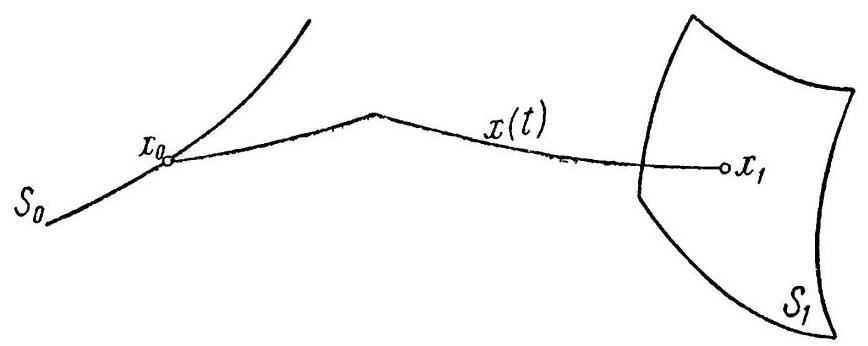
\includegraphics[max width=0.8\textwidth]{images/bo_d547imjef24c73bgfcdg_56_341_637_868_346_0.jpg}
\end{center}
\hspace*{3em}

Pnc. 20.

Однако нужно в этом случае иметь еще соотноше- ния, из которых можно было бы определить поло- жение точек \({x}_{0},{x}_{1}\) на многообразиях 8, \({S}_{0}\), \({S}_{1}\). Ta- кими соотношениями и являются формулируемые в этом параграфе условия трансверсальности. Эти условия позволяют написать \({r}_{0} + {r}_{1}\) соотношений, включающих координаты концевых точек \({x}_{0}\) и \({x}_{1}\). Так как, с другой стороны, число неизвестных парамет- ров (по сравнению с задачей с закрепленными концами) также увеличилось на \({r}_{0} + {r}_{1}\) (ибо положение точки \({x}_{0}\) на \({r}_{0}\) -мерном многообразии \({S}_{0}\) характеризуется \({r}_{0}\) параметра- ми, a положение точки \({x}_{1} \in  {S}_{1}\) характеризуется \({r}_{1}\) пара- метрами), то вместе с принципом максимума условия трансверсальности образуют «достаточную» систему соотно- шений для решения поставленной оптимальной задачи с подвижными концами.

Приведем теперь формулировку условий трансверсаль- ности. Пусть \({x}_{0} \in  {S}_{0}\), \({x}_{1} \in  {S}_{1}\) - некоторые точки, a \({T}_{0}\) и \({T}_{1}\) — касательные плоскости многообразий \({S}_{0}\) и \({S}_{1}\), проведенные в этих точках. Плоскости \({T}_{0}\) и \({T}_{1}\) расположены в пространстве \(X\) и имеют размерности соответственно \({r}_{0},{r}_{1}\). Пусть,далее, \(u\left( t\right),x\left( t\right),{t}_{0} \leq  t \leq  {t}_{1}\),- решение оптимальной задачи с закрепленными концами и, и и и) и Наконец, пусть ψ (t) — вектор, существование которого утверждается в теореме 1. Мы будем говорить, что век- тор ψ (t) удовлетворяет условию трансверсальности в правом конце траектории \(x\left( t\right)\) (т. e. в точке \(x\left( {t}_{1}\right)\) ), если вектор \(\psi \left( {t}_{1}\right)  = \left( {{\psi }_{1}\left( {t}_{1}\right),{\psi }_{2}\left( {t}_{1}\right),\ldots,{\psi }_{n}\left( {t}_{1}\right) }\right)\) ортогонален плоскости \({T}_{1}\). Иначе говоря, условие трансверсальности означает, что для любого вектора в = (0', 0'' …, 0'), принадлежащего (или параллельного) плоскости Т, вы- полнено соотношение (ψ (t, θ) = 0. Аналогичный смысл имеет условие трансверсальности в л е в о м конце траектории \(x\left( t\right)\) (нужно лишь заменить \({t}_{1}\) и \({T}_{1}\) на \({t}_{0}\) и \({T}_{0}\) соответственно). Ясно, что условие трансверсальности в правом конце траектории \(x\left( t\right)\) содержит \({r}_{1}\) независимых соотношений, ибо в соотношение (ψ (t, ) н) = 0 достаточно подставить \({r}_{1}\) линейно независимых векторов \({\theta }_{1},{\theta }_{2},\ldots \; \ldots,{\theta }_{{r}_{1}}\), расположенных в плоскости \({T}_{1}\). Условие транс- версальности в левом конце содержит \({r}_{0}\) независимых соотношений.

Пользуясь условиями трансверсальности, можно сформулировать теперь решение задачи с подвижными концами.

T e o p e м a 3. Пусть и (t), \({t}_{0} \leq  t \leq  {t}_{1}\),— допустимое управление, переводящее фазовую точку из некоторого положения \({x}_{0} \in  {S}_{0}\) в положение \({x}_{1} \in  {S}_{1},a\mathbf{x}\left( t\right)  -\) соответ- ствующая траектория (исходящая из точки хво, = (0, ио). Для того чтобы и (t) и х (t) давали решение оптималь- ной задачи с подвижными концами, необходимо су- ществование ненулевой непрерывной вектор-функции ψ (t), удовлетворяющей условиям, указанным в теореме 1, и, кроме того, условию трансверсальности в обоих концах траектории \(x\left( t\right)\).

Разумеется, если одно из многообразий \({S}_{0},{S}_{1}\) вырож- дается в точку, то условие трансверсальности в соответ- ствующем конце траектории \(x\left( t\right)\) заменяется условием прохождения траектории \(x\left( t\right)\) через эту точку.

Для случая оптимальности по быстродействию в фор- мулировке теоремы 3 решение \(x\left( t\right)\) заменяется на \(x\left( t\right)\),

му 2.

Приведем элементарные примеры решения задач с под- вижными концами.

\section*{Пример 1}

Рассмотрим для точки, движущейся по закону (22) (с тем же ограничением | и | ≤ 1), задачу о быстрейшем попадании на ось \({x}^{2}\) из заданного начального состояния \({x}_{0}\). В этом случае мы имеем задачу с подвижным пра- вым концом: многообразие \({S}_{0}\) вырождается в точку \({x}_{0}\), а многообразием S1 служит \({x}^{1} = 0\). Вектор \(\theta  = \left( {{\theta }^{1},{\theta }^{2}}\right)\), касающийся многообразия \({S}_{1}\) (в любой его точке), имеет вид не (0, \({\theta }^{2}\) ), где \({\theta }^{2} \neq  0\) и, следовательно, ус- ловие трансверсальности в правом конце записывается в форме 0. \({\psi }_{1}\left( {t}_{1}\right)  + {\theta }^{2}{\psi }_{2}\left( {t}_{1}\right)  = 0\), откуда — \({\psi }_{2}\left( {t}_{1}\right)  = 0\). Так как по-прежнему функция \({\psi }_{2}\left( t\right)\) пинейна (см. стр. 29), то из соотношения \({\psi }_{2}\left( {t}_{1}\right)  = 0\) вытекает,что \({\psi }_{2}\left( t\right)\) сохраняет постоянный знак при \({t}_{0} \leq  t < {t}_{1}\). Таким образом (см. (24)),в этом случае каждое оптимальное управление \(u\left( t\right)\) п о с т о я н н о и равно +1 или -1, и потому оптимальными могут быть только движения по параболам (25), (26) (без переключе- ний). Предположим сначала, что начальное фазовое состоя- ние \({x}_{0}\) находится с п р а в а от прямой и" = 0. Согласно сказанному выше, через точку и проходят только две фазовые траектории, которые могут оказаться оптималь- ными: траектория (25), по которой движение происходит снизу вверх, и траектория (26), по которой движение происходит сверху вниз (рис. 21). Если точка х, распо- ложена выше линии АО (см. рис. 7), то, двигаясь по параболе (25), фазовая точка не попадет на ось х" = 0 (рис. 22a), и потому оптимальным может быть только дви- жение по параболе (26). Если же точка хор асположена на линии АО или ниже нее, то оба движения (25), (26) приводят фазовую точку на ось и" = 0 (рис. 226). Итак, в этом случае имеются д в е траектории, удовлет- воряющие принципу макси- мума. Однако легко видеть, что время движения по этим траекториям из точки \({x}_{0}\) до оси из = 0 различно. Действи- тельно, проведя касательные к параболам (25) и (26) в точ- ке \({x}_{0}\),мы легко найдем (см. puc. 23), что \({Q}_{0}{Q}_{2} > {Q}_{0}{P}_{2} = \; = {Q}_{0}{P}_{1} > {Q}_{0}{Q}_{1}\), a так как при \(u =  \pm  1\) время движения по дуге параболы равно раз- ности ординат (см. второе уравнение (22)), то движение по дуге \({x}_{0}{Q}_{2}\) происходит д о л ь ш е, чем по дуге \({x}_{0}{Q}_{1}\). Ta- ким образом, и в этом случае оптимальным может быть

\begin{center}
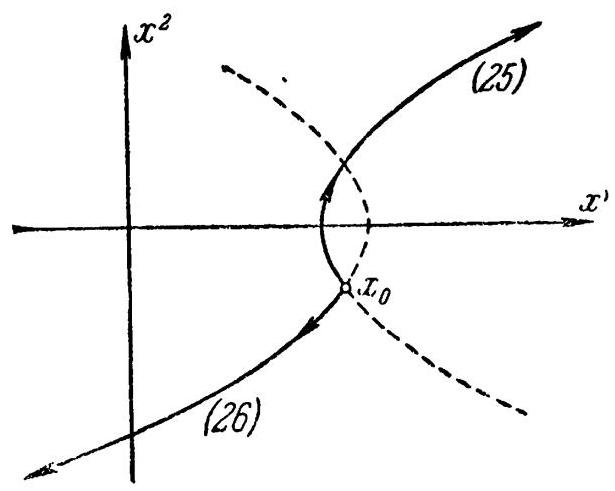
\includegraphics[max width=0.5\textwidth]{images/bo_d547imjef24c73bgfcdg_58_798_737_615_491_0.jpg}
\end{center}
\hspace*{3em}

Puc. 21

\begin{center}
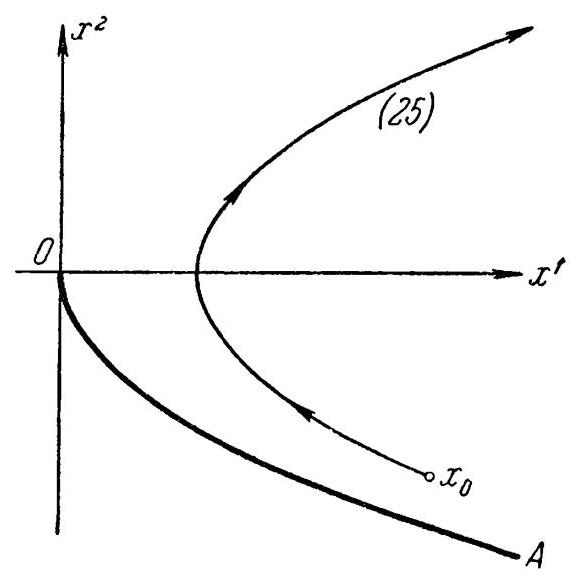
\includegraphics[max width=0.5\textwidth]{images/bo_d547imjef24c73bgfcdg_59_134_367_577_576_0.jpg}
\end{center}
\hspace*{3em}

Pac. 22a.

\begin{center}
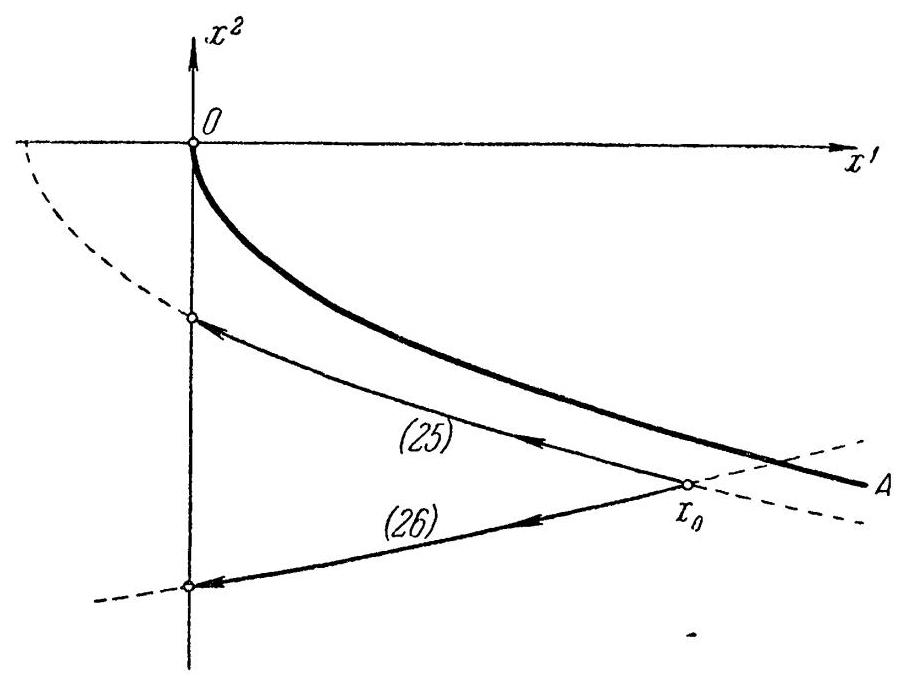
\includegraphics[max width=0.8\textwidth]{images/bo_d547imjef24c73bgfcdg_59_306_1165_904_677_0.jpg}
\end{center}
\hspace*{3em}

Prac. 226.

только движение по траектории (26). Итак, в правой полу- плоскости оптимальными могут быть только движения по параболам (26), т. е. движения, совершающиеся при \(u =  - 1\). Аналогично, слева от оси и 1 = 0 оптимальными могут быть только движения по параболам (25), т. е. движения, совершающиеся при и == + 1. Это и дает син- тез оптимальных управлений: положив

\[
v\left( {{x}^{1},{x}^{2}}\right)  = \left\{  \begin{array}{l}  + 1\text{ при }{x}^{1} < 0, \\   - 1\text{ при }{x}^{1} > 0, \end{array}\right.
\]

\begin{center}
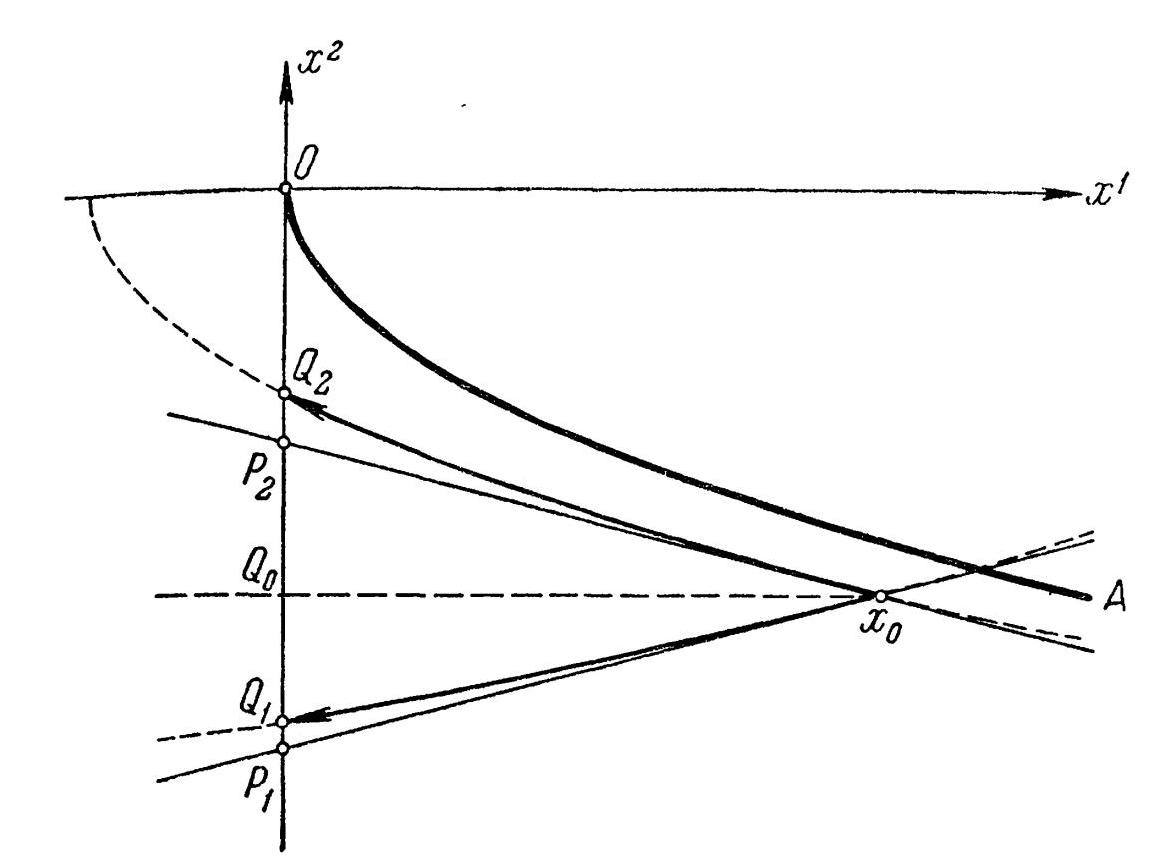
\includegraphics[max width=1.0\textwidth]{images/bo_d547imjef24c73bgfcdg_60_177_233_1173_857_0.jpg}
\end{center}
\hspace*{3em}

Puc. 23.

\begin{center}
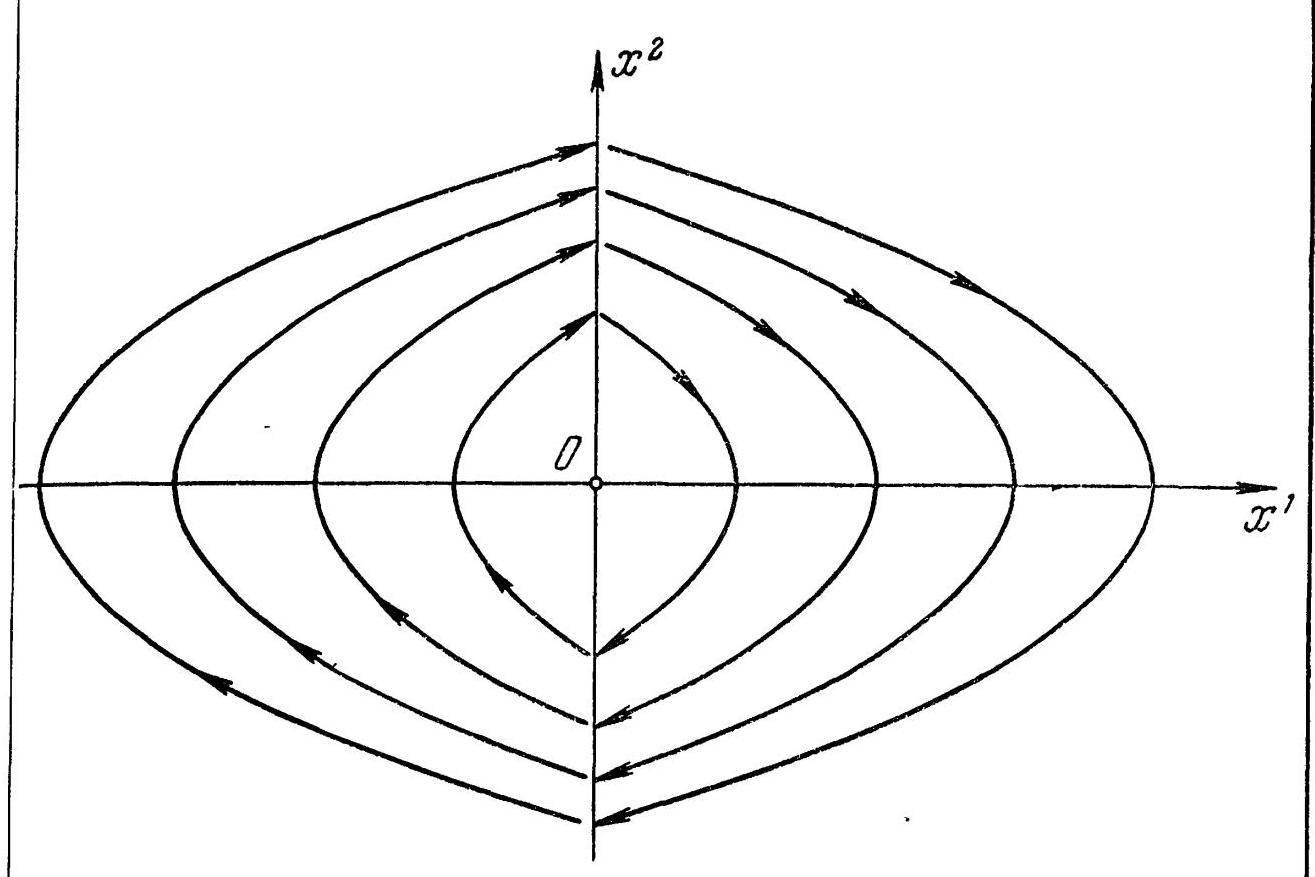
\includegraphics[max width=1.0\textwidth]{images/bo_d547imjef24c73bgfcdg_60_102_1174_1315_877_0.jpg}
\end{center}
\hspace*{3em}

Prac. 24.

мы получим совокупность всех оптимальных траекторий из системы

\[
\left. \begin{array}{l} \frac{d{x}^{1}}{dt} = {x}^{2}, \\  \frac{d{x}^{2}}{dt} = v\left( {{x}^{1},{x}^{2}}\right)  \end{array}\right\} \tag{51}
\]

(cp. (27)). Фазовая картина оптимальных траекторий изображена на рис. 24.

Уравнения (51) можно, впрочем, считать очевидными (например, с механической точки зрения).

\(\Pi\) p \(u\) м е р 2

Рассмотрим для точки, движущейся по закону (28) (с тем же ограничением | и | ≤ 1), задачу о быстрейшем попадании на окружность

\[
{\left( {x}^{1}\right) }^{2} + {\left( {x}^{2}\right) }^{2} = {R}^{2} \tag{52}
\]

из заданного начального состояния \({x}_{0}\),находящегося вне этой окружности. В этом случае мы также имеем задачу с подвижным правым концом: многообразием S1 служит ок- ружность (52). Пусть \({x}_{1} = \left( {R\cos \alpha,R\sin \alpha }\right)  -\) произвольная точка окружности (52). Найдем оптимальную траекторию, дающую решение поставленной задачи с подвижным пра- вым концом и оканчивающуюся в точке х, в качестве \(\psi \left( {t}_{1}\right)\),т. e. вектора, нормального к окружности (52) в точке х, (в силу условий трансверсальности), мы должны взять один из двух векторов (— \(\cos \alpha, - \sin \alpha\) ), \(\left( {\cos \alpha,\sin \alpha }\right)\), первый из которых направлен внутрь окружности, а вто- рой — в обратную сторону. Так как искомая оптималь- ная траектория должна подходить к точке \({x}_{1}\), распола- гаясь в н е окружности (52), то вектор фазовой скорости \(f\left( {x\left( {t}_{1}\right),u\left( {t}_{1}\right) }\right)\) в точке \(x\left( {t}_{1}\right)  = {x}_{1}\) будет направлен либо внутрь окружности (52), либо по касательной к этой окружности в точке хз наше скалярное произведение

\[
\left( {\psi \left( {t}_{1}\right) ,f\left( {x\left( {t}_{1}\right) ,u\left( {t}_{1}\right) }\right) }\right)  = H\left( {\psi \left( {t}_{1}\right) ,x\left( {t}_{1}\right) ,u\left( {t}_{1}\right) }\right) \tag{53}
\]

должно быть неотрицательным (см. теорему 2 и, в част- ности, соотношение (21)), мы находим, что в качестве \(\psi \left( {t}_{1}\right)\) следует взять вектор (— cos α,— sin α), направлен- ный по радиусу внутрь окружности. (Если вектор фазо- вой скорости \(f\left( {x\left( {t}_{1}\right),u\left( {t}_{1}\right) }\right)\) окажется направленным по касательной к окружности, то скалярное произведение (53) будет равно нулю, и потому в качестве ψ (t1) можно взять как вектор, направленный внутрь окружности, так и про- тивоположно направленный вектор; в целях единообразия мы и в этом случае условимся считать ψ (t1) направлен- ным внутрь окружности.) Итак, мы имеем:

\[
\psi \left( {t}_{1}\right)  = \left( {-\cos \alpha , - \sin \alpha }\right) .
\]

\begin{center}
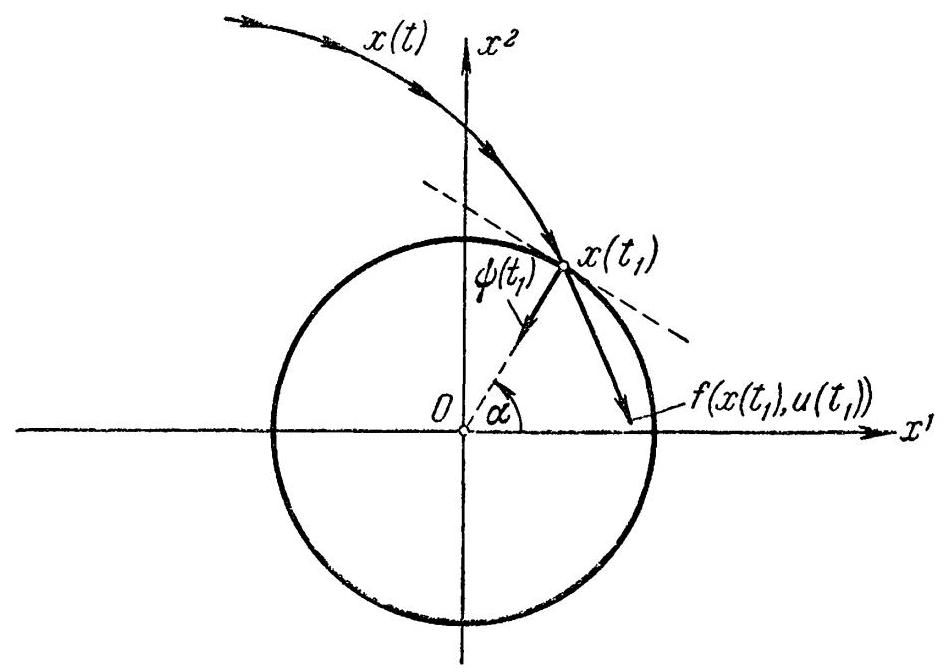
\includegraphics[max width=0.8\textwidth]{images/bo_d547imjef24c73bgfcdg_62_290_667_949_672_0.jpg}
\end{center}
\hspace*{3em}

Puc. 25.

Вспоминая теперь систему уравнений (см. стр. 34)

\[
\frac{d{\psi }_{1}}{dt} = {\psi }_{2},\;\frac{d{\psi }_{2}}{dt} =  - {\psi }_{1}
\]

для нахождения вектор-функции \(\psi \left( t\right)  = \left( {{\psi }_{1}\left( t\right),{\psi }_{2}\left( t\right) }\right)\),мы получаем окончательно

\({\psi }_{1}\left( t\right)  =  - \cos \left( {t - {t}_{1} - \alpha }\right) ,\;{\psi }_{2}\left( t\right)  = \sin \left( {t - {t}_{1} - \alpha }\right) ,\)

\[
{t}_{0} \leq  t \leq  {t}_{1}.
\]

Соотношение (20) дает нам (учитывая (29) и условие \(\left| u\right|  \leq  1)\) :

\[
u = \operatorname{sign}{\psi }_{2} = \operatorname{sign}\left( {\sin \left( {t - {t}_{1} - \alpha }\right) }\right) . \tag{54}
\]

Если угол \(\alpha\) удовлетворяет неравенствам 0 ≤ α < π, то на отрезке \({t}_{1} - \left( {\pi  - \alpha }\right)  \leq  t \leq  {t}_{1}\) управление \(u\left( t\right)\) будет,

\begin{center}
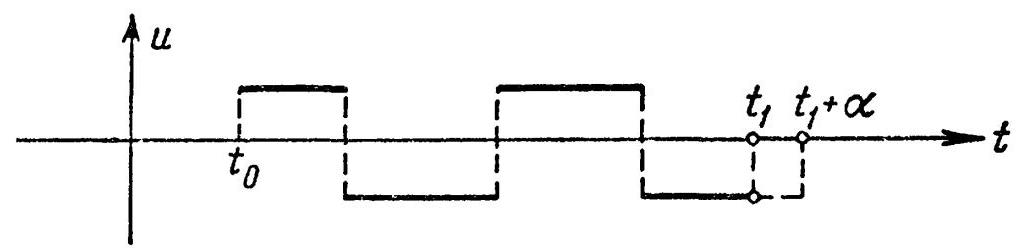
\includegraphics[max width=0.9\textwidth]{images/bo_d547imjef24c73bgfcdg_63_251_520_1026_252_0.jpg}
\end{center}
\hspace*{3em}

Prac. 26.

в силу (54), равно — 1, а перед этим будет попеременно равно + 1 и - 1 на отрезках длины π (рис. 26). Таким образом, последний кусок фазовой траектории (оканчи- вающийся в точке и, представляет собой дугу окруж- ности с центром в точке (— 1, 0), причем эта дуга соот- ветствует центральному углу π — α, а предшествующие куски фазовой траектории являются полуокружностями попеременно с центрами в точках (1, 0) и (- 1,0). Вид фазовой траектории показан на рпс. 27. Если же угол а удовлетворяет неравенствам π ± α < 2π, то траектория, изображенная на рис. 27, заменяется центрально симме- тричной. Легко видеть (см. рис. 28), что при 0 ≤ α < π конец \(B\) последней дуги \({BA}\) рассматриваемой оптималь- ной траектории расположен на окружности радиуса 1 c центром в точке ( — R — 1, 0). При изменении а от 0 до π точка B описывает половину \({\mathrm{N}}_{2}{\mathrm{\;N}}_{1}\) этой окружности, расположенную над осью абсцисс. Далее, предыдущий кусок CB оптимальной траектории представляет собой полуокружность с центром в точке (1, 0), и потому конец C этой полуокружности лежит на полуокружности \({M}_{2}{M}_{3}\), которая симметрична \({N}_{1}{N}_{2}\) относительно центра (1,0). Продолжая таким образом, мы и получим всю фазовую траекторию (рис. 29). Аналогично строится центрально симметричная траектория. Общее расположение фазовых траекторий показано на рис. 30.

\begin{center}
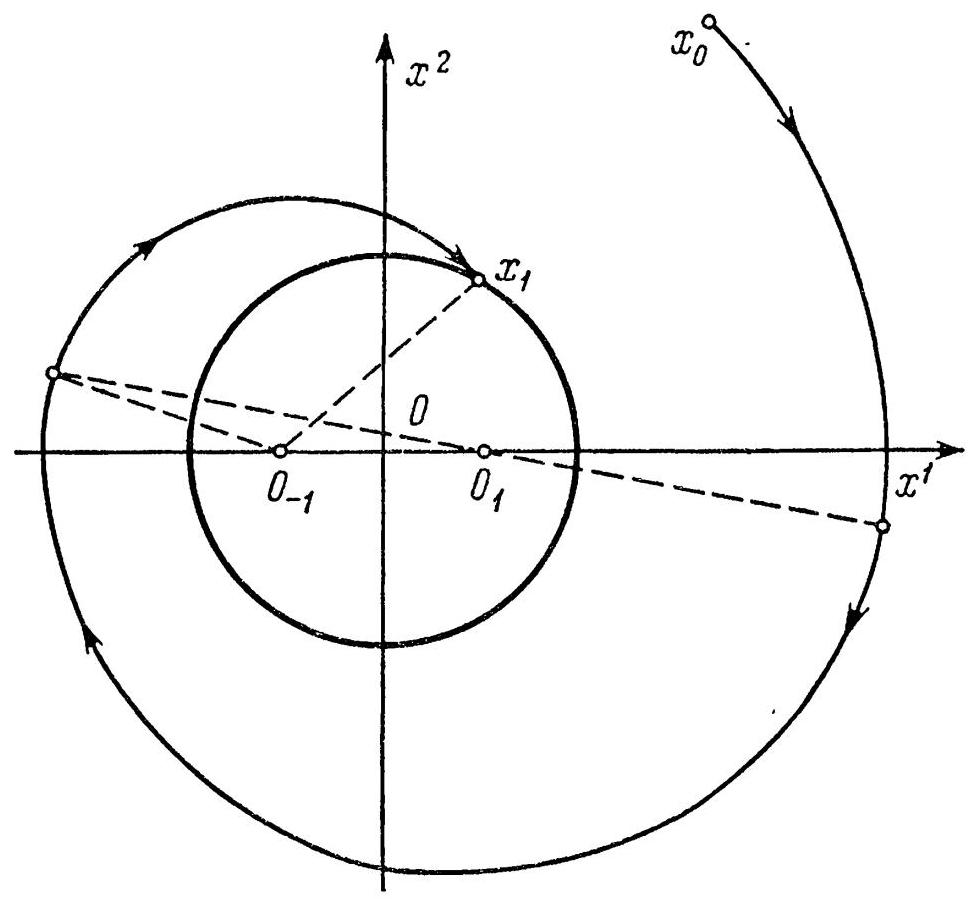
\includegraphics[max width=0.9\textwidth]{images/bo_d547imjef24c73bgfcdg_63_274_1006_976_901_0.jpg}
\end{center}
\hspace*{3em}

Prac. 27.

\begin{center}
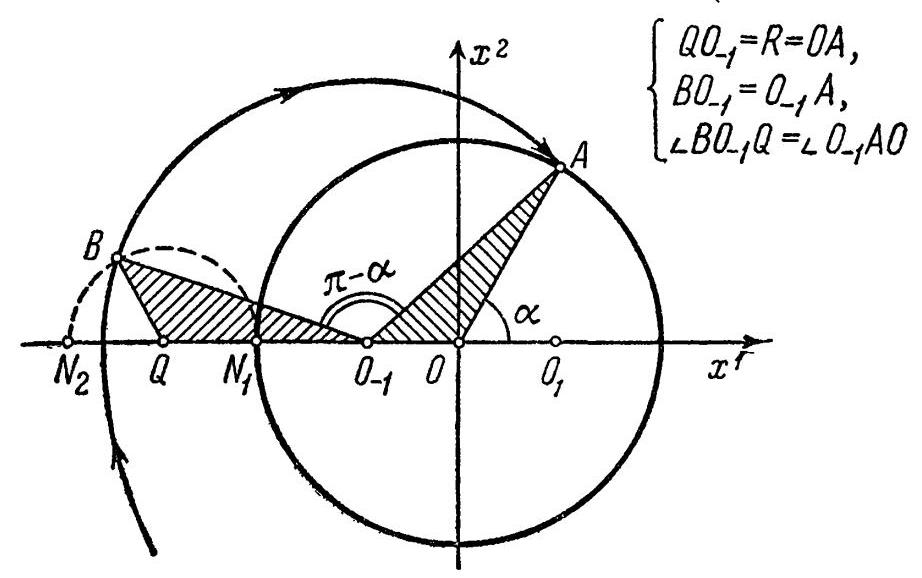
\includegraphics[max width=0.8\textwidth]{images/bo_d547imjef24c73bgfcdg_64_304_308_922_578_0.jpg}
\end{center}
\hspace*{3em}

Pac. 28.

\begin{center}
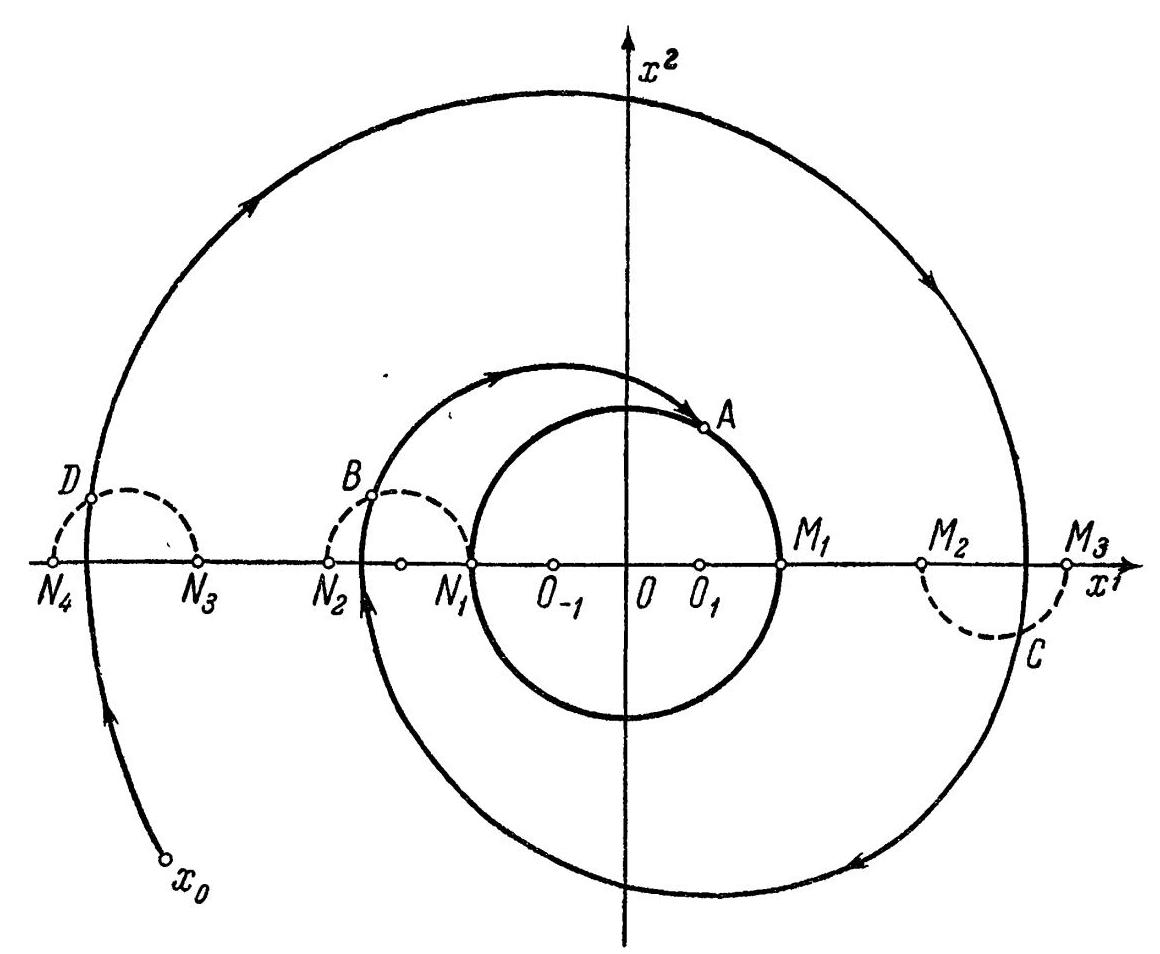
\includegraphics[max width=1.0\textwidth]{images/bo_d547imjef24c73bgfcdg_64_179_1020_1160_954_0.jpg}
\end{center}
\hspace*{3em}

Prac. 29.

3 Л. С. Понтрягин и др.

\begin{center}
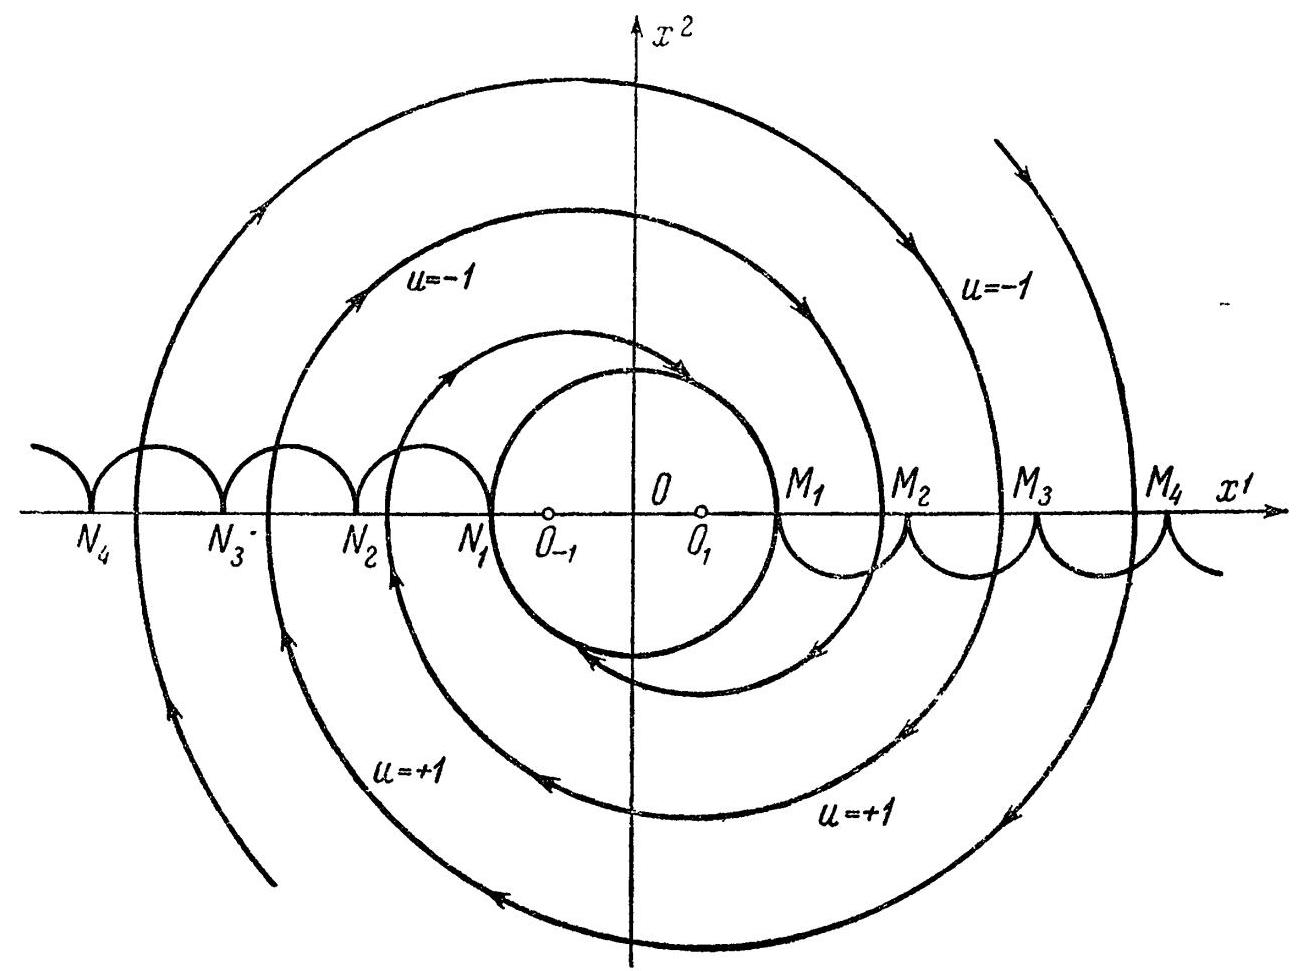
\includegraphics[max width=1.0\textwidth]{images/bo_d547imjef24c73bgfcdg_65_111_514_1302_971_0.jpg}
\end{center}
\hspace*{3em}

Pnc. 30.

Синтез оптимальных управлений осуществляется функ- пией \(v\left( {{x}^{1},{x}^{2}}\right)\),которая строится, как вытекает из пре- лыдущего, следующим образом. К окружности (52) при- кладываются справа равные между собой полуокружности \({M}_{1}{M}_{2},{M}_{2}{M}_{3},\ldots\) радиуса 1, расположенные под осью абсписс. Слева от окружности (52) строятся аналогичные полуокружности \({N}_{1}{N}_{2},{N}_{2}{N}_{3},\ldots\), расположенные над осью абсписс. Функция у (x'1, x'2) определяется теперь вне окружности (52): \(v\left( {{x}^{1},{x}^{2}}\right)\) равна +1 ниже линии \(\ldots {N}_{2}{N}_{1}{M}_{1}{M}_{2}\ldots\) и равна —1 выше линии \(\ldots {M}_{2}{M}_{1}{N}_{1}{N}_{2}\ldots {\theta }_{\mathrm{{TO}}}\) и дает синтез оптимальных управ- лений:

\[
\left. \begin{array}{l} \frac{d{\mathbf{x}}^{\mathbf{1}}}{dt} = {x}^{2}, \\  \frac{d{\mathbf{x}}^{\mathbf{2}}}{dt} =  - {x}^{1} + v\left( {{x}^{1},{x}^{2}}\right) . \end{array}\right\}
\]

\section*{§ 7. Принцип максимума для неавтономных систем}

A. Рассмотрим оптимальную задачу такого же вида, как 11 (4), (7), но в случае, когда функции f" явно зависят от времени (область управления \(U\) предполагается не за- висящей от времени). Таким образом, закон движения объекта и функционал, минимум которого ищется, прини- мают в рассматриваемом случае вид

\[
\frac{d{x}^{i}}{dt} = {f}^{i}\left( {x,u,t}\right) ,\;i = 1,2,\ldots ,n; \tag{55}
\]

\[
J = {\int }_{{t}_{0}}^{{t}_{1}}{f}^{0}\left( {x\left( t\right) ,u\left( t\right) ,t}\right) {dt} \tag{56}
\]

Время бо здесь предполагается заданным, а б1 — искомое время прохождения через точку и введя, как и прежде, новую координату \({x}^{0} = {\int }_{{t}_{0}}^{t}{f}^{0}\left( {x\left( t\right),u\left( t\right),t}\right) {dt}\),мы сформу- лируем рассматриваемую задачу в следующей форме (cp. \(\text{ § }2\) ).

B (n + 1)-мерном фазовом пространстве X даны точка \({x}_{0} = \left( {0,{x}_{0}}\right)\) и прямая П, параллельная оси и проходящая через точку (0, \({x}_{1}\) ). Среди всех допустимых управлений \(u = u\left( t\right)\), обладающих тем свойством, что соответству- ющее решение х (t) системы

\[
\frac{d{x}^{i}}{dt} = {f}^{i}\left( {x,u,t}\right) ,\;i = 0,1,\ldots ,n, \tag{57}
\]

c начальным условием x(t,0) = x0 пересекает прямую П, найти такое, для которого точка пересечения с прямой П имеет наименьшую координату х0.

Для решения этой задачи введем еще одно вспомога- тельное неизвестное \({x}^{n + 1}\), изменяющееся по закону

\[
\frac{d{x}^{n + 1}}{dt} = 1,\;{x}^{n + 1}\left( {t}_{0}\right)  = {t}_{0}.
\]

Очевидно, что мы будем иметь \({x}^{n + 1} \equiv  t\). Пространство переменных \({x}^{1},{x}^{2},\ldots,{x}^{n},{x}^{n + 1}\) обозначим через X*. C помощью неизвестного хити система (57) может быть записана в следующем автономном (т.е. не зависящем явно от t) виде:

\[
\left. \begin{aligned} \frac{d{x}^{i}}{dt} &  = {f}^{i}\left( {x,u,{x}^{n + 1}}\right) ,\;i = 0,1,\ldots ,n, \\  \frac{d{x}^{n + 1}}{dt} &  = 1. \end{aligned}\right\}
\]

При этом мы должны найти оптимальную траекторию, соединяющую в пространстве X* точку ( \({x}_{0}^{1},{x}_{0}^{2},\ldots,{x}_{0}^{n},{t}_{0}\) ) c некоторой точкой прямой \({S}_{1}\), проходящей через точку \(\left( {{x}_{1}^{1},{x}_{1}^{2},\ldots,{x}_{1}^{n},0}\right)\) параллельно оси \({x}^{n + 1}\) (ибо конечное значе- ние переменного \({x}^{n + 1}\), т. е. момент времени, когда движу- щаяся точка приходит в положение и, не является заранее заданным). Таким образом, мы приходим к обычной опти- мальной задаче с закрепленным левым концом и подвиж- ным правым концом.

Напишем принцип максимума и условие трансверсаль- ности для полученной задачи. Вспомогательная система уравнений (12) имеет вид

\[
\frac{d{\psi }_{i}}{dt} =  - \mathop{\sum }\limits_{{\alpha  = 0}}^{n}\frac{\partial {f}^{\alpha }}{\partial {x}^{i}}{\psi }_{\alpha },\;i = 0,1,\ldots ,n, \tag{58}
\]

\[
\frac{d{\psi }_{n + 1}}{dt} =  - \mathop{\sum }\limits_{{\alpha  = 0}}^{n}\frac{\partial {f}^{\alpha }}{\partial t}{\psi }_{\alpha } \tag{59}
\]

Согласно теоремам 1 и 3, для решения рассматриваемой задачи нужно составить функцию

\[
{\psi }_{0}{f}^{0}\left( {x,u,{x}^{n + 1}}\right)  + {\psi }_{1}{f}^{1}\left( {x,u,{x}^{n + 1}}\right)  + \ldots
\]

\[
\cdots  + {\psi }_{n}{f}^{n}\left( {x,u,{x}^{n + 1}}\right)  + {\psi }_{n + 1} \cdot  1.
\]

Эту функцию мы обозначим через Ж* (а не через Ж, как в теореме 1), сохранив обозначение Ж для функции \(\mathcal{K}\left( {\psi,x,t,u}\right)  = {\psi }_{0}{f}^{0}\left( {x,u,t}\right)  + {\psi }_{1}{f}^{1}\left( {x,u,t}\right)  + \ldots\)

\[
\ldots  + {\psi }_{n}{f}^{n}\left( {x,u,t}\right)
\]

с помощью которой уравнения (57), (58) записываются в виде гамильтоновой системы

\[
\frac{d{x}^{i}}{dt} = \frac{\partial \mathcal{K}}{\partial {\psi }_{i}},\;\frac{d{\psi }_{i}}{dt} =  - \frac{\partial \mathcal{K}}{\partial {x}^{i}},\;i = 0,\ldots ,n.
\]

Точно так же максимум по и функции Ж * при фикси- рованных \({x}^{i},{\psi }_{i}\) мы обозначим через M* (ψ, х, х*-1) (а не через \(\mathcal{M}\), как в теореме 1), сохранив обозначение \(\mathcal{A}\left( {\psi,x,t}\right)\) для максимума (по и) функции \(\mathcal{K}\left( {\psi,x,t,u}\right)\) при фиксированных ф, х, t. Таким образом, учитывая соотношение \({x}^{n + 1} \equiv  t\),мы можем написать \({\mathcal{K}}^{ * } = \mathcal{K} + {\psi }_{n + 1}\), \({\mathcal{M}}^{ * } = \mathcal{M} + {\psi }_{n + 1}\),и потому соотношение Ж* = М* = 0, выполняющееся вдоль оптимальной траектории (см. теоре- му 1), принимает вид

\[
\mathcal{K}\left( {\psi \left( t\right) ,x\left( t\right) ,t,\dot{u}\left( t\right) }\right)  = \mathcal{M}\left( {\psi \left( t\right) ,x\left( t\right) ,t}\right)  \equiv   - {\psi }_{n + 1}\left( t\right) . \tag{60}
\]

Наконец, условие трансверсальности в правом конце траектории показывает, что прямая \({S}_{1}\) (параллельная осп \({x}^{n + 1}\) ) ортогональна вектору ( \({\psi }_{1}\left( {t}_{1}\right),{\psi }_{2}\left( {t}_{1}\right),\ldots,{\psi }_{n + 1}\left( {t}_{1}\right)\) ). Иначе говоря, \({\psi }_{n + 1}\left( {t}_{1}\right)  = 0\). Вместе с соотношениями (60), (59) это дает нам

\[
\mathcal{M}\left( {\psi \left( t\right) ,x\left( t\right) ,t}\right)  = {\int }_{{t}_{1}}^{t}\mathop{\sum }\limits_{{\alpha  = 0}}^{n}\frac{\partial {f\alpha }\left( {x\left( t\right) ,u\left( t\right) ,t}\right) }{\partial t}{\psi }_{\alpha }\left( t\right) {dt}.
\]

Итак, мы получаем следующую теорему (принцип максимума для неавтономных систем).

T e o p e m a 4. Пусть и (t), t, s e t ≤ t, - такое допу- стимое управление, что соответствующая ему траектория \(x\left( t\right)\) систеты (57), исходящая в момент \({t}_{0}\) из точки х, проходит в момент н1 через некоторую точку прямой П. Для оптимальности управления и (t) и траектории x (t) необходимо существование такой ненулевой непрерывной вектор-функции \(\psi \left( t\right)  = \left( {{\psi }_{0}\left( t\right),{\psi }_{1}\left( t\right),\ldots,{\psi }_{n}\left( t\right) }\right),\) соответ- ствующей функциям и (t) и х (t) (см. (58)), что:

\({1}^{ \circ  }\) для всех t, \({t}_{0} \leq  t \leq  {t}_{1}\) ,функция \(\mathcal{K}\left( {\psi \left( t\right) ,x\left( t\right) ,t,u}\right)\) переменного \(u \in  U\) достигает в точке и = и (t) максимума

\[
\mathcal{K}\left( {\psi \left( t\right) ,x\left( t\right) ,t,u\left( t\right) }\right)  = \mathcal{M}\left( {\psi \left( t\right) ,x\left( t\right) ,t}\right) ; \tag{61}
\]

2 \textdegree  выполнены соотношения

\[
{\psi }_{0}\left( t\right)  = \text{ const } \leq  0
\]

\[
\mathcal{M}\left( {\psi \left( t\right) ,x\left( t\right) ,t}\right)  = {\int }_{{t}_{1}}^{t}\mathop{\sum }\limits_{{\alpha  = 0}}^{n}\frac{\partial {f}^{\alpha }\left( {x\left( t\right) ,u\left( t\right) ,t}\right) }{\partial t}{\psi }_{\alpha }\left( t\right) {dt}. \tag{62}
\]

Оказывается, далее, что если величины ψ(t), x (t), и (t) удовлетворяют системе (57), (58) и условию 1 \textdegree, то функция \({\psi }_{0}\left( t\right)\) переменного t постоянна, а функция \(\mathcal{A}\left( {\psi \left( t\right),\;x\left( t\right),\;t}\right)\) может лишь на константу отличаться от интеграла, указанного во втором соотношении (62), так что проверку соотношений (62) достаточно произвести лишь в какой-либо один момент времени t, t, 6 ≤ t ≤ t; например, вместо (62) достаточно проверить соотно- шения

\[
{\psi }_{0}\left( {t}_{1}\right)  \leq  0,\;\mathcal{M}\left( {\psi \left( {t}_{1}\right) ,x\left( {t}_{1}\right) ,{t}_{1}}\right)  = 0. \tag{63}
\]

Б. Если теперь предположить, что точка х, в которую точка \({x}_{0}\) должна переводиться с помощью управления \(u\left( t\right)\), не неподвижна, a перемещается,т. е. \({x}_{1} = {x}_{1}\left( t\right)\),то фор- мулировка теоремы 4 несколько меняется. Именно, пусть \(u\left( t\right),{t}_{0} \leq  t \leq  {t}_{1}, - \operatorname{raxo}\) допустимое управление,которое точку \({x}_{0}\) в некоторый момент времени и приводит в точку \({x}_{1}\left( {t}_{1}\right)\),и пусть \({\left. \frac{d{x}_{1}}{dt}\right| }_{t = {t}_{1}} = \left( {{q}^{1},{q}^{2},\ldots,{q}^{n}}\right)\) - касательный вектор к кривой и (1) в момент и. Тогда, после введения вспомогательного переменного \({x}^{n + 1} \equiv  t\),мы получим,что многообразие \({S}_{1}\) будет уже не прямой, параллельной ocu \({x}^{n + 1}\), a линией \(\left( {{x}_{1}^{1}\left( \theta \right),{x}_{1}^{2}\left( \theta \right),\ldots,{x}_{1}^{n}\left( \theta \right),\theta ),\mathrm{{rde}}\theta  - }\right.\) mapamerp. Kacarenblaz groß inhibit b toke \(\theta  = {t}_{1}\) определяется вектором \(\left( {{q}^{1},{q}^{2},\ldots,{q}^{n},1}\right)\), \(\mathbf{u}\) потому условие трансверсальности принимает вид

\[
\mathop{\sum }\limits_{{v = 1}}^{n}{\psi }_{v}\left( {t}_{1}\right) {q}^{v} + {\psi }_{n + 1}\left( {t}_{1}\right)  \cdot  1 = 0
\]

Отсюда, учитывая соотношение (60), получаем

\[
\mathcal{M}\left( {\psi \left( {t}_{1}\right) ,x\left( {t}_{1}\right) ,{t}_{1}}\right)  =  - {\psi }_{n + 1}\left( {t}_{1}\right)  = \mathop{\sum }\limits_{{v = 1}}^{n}{\psi }_{v}\left( {t}_{1}\right) {q}^{v}.
\]

Так как, наконец, согласно (60) и (59), функция \(\mathcal{M}\left( {\psi \left( t\right),x\left( t\right),t}\right)\) является первообразной для

\[
\mathop{\sum }\limits_{{\alpha  = 0}}^{n}\frac{\partial {f\alpha }\left( {x\left( t\right) ,u\left( t\right) ,t}\right) }{\partial t}{\psi }_{\alpha }\left( t\right) ,
\]

TO MEI IOJIYYACM

\[
\mathcal{M}\left( {\psi \left( t\right) ,x\left( t\right) ,t}\right)  =
\]

\[
= \mathop{\sum }\limits_{{v = 1}}^{n}{\psi }_{v}\left( {t}_{1}\right) {q}^{v} + {\int }_{{t}_{1}}^{t}\mathop{\sum }\limits_{{\alpha  = 0}}^{n}\frac{\partial {f}^{\alpha }\left( {x\left( t\right) ,u\left( t\right) ,t}\right) }{\partial t}{\psi }_{\alpha }\left( t\right) {dt}. \tag{64}
\]

Это и есть соотношение, которым необходимо заменить вто- рое из равенств (62) в формулировке теоремы 4; в связи с этим соотношения (63) принимают вид

\[
{\psi }_{0}\left( {t}_{1}\right)  \leq  0,\;\mathcal{M}\left( {\psi \left( {t}_{1}\right) ,x\left( {t}_{1}\right) ,{t}_{1}}\right)  = \mathop{\sum }\limits_{{v = 1}}^{n}{\psi }_{v}\left( {t}_{1}\right) {q}^{v}. \tag{65}
\]

В остальном же формулировка теоремы 4 сохраняется.

B. Наконец, рассмотрим неавтономную оптимальную за- дачу с подвижными концами. Ограничимся случаем под- вижного правого конца. Пусть \({S}_{1}\left( t\right)\) - перемещающееся \(r\) -мерное многообразие, дифференцируемым образом зави- сящее от t. Задача заключается в отыскании такого до- пустимого управления \(u\left( t\right),{t}_{0} \leq  t \leq  {t}_{1}\),что точка,движу- щаяся по закону (55) с начальным условием x ( \({t}_{0}\) ) = x0, попадает в некоторый момент \({t}_{1}\) на многообразие \({S}_{1}\left( {t}_{1}\right)\), причем осуществляется минимум функционала (56).

Уточним прежде всего понятие «перемещающегося многообразия». Пусть в ( \(n + 1\) )-мерном пространстве переменных \({x}^{1},{x}^{2},\ldots,{x}^{n}\), \(t\) рассматривается \(\left( {r + 1}\right)\) - мерное многообразие \({S}_{1}^{ * }\), определяемое системой урав- нений

\[
\left. \begin{array}{r} {f}_{1}\left( {{x}^{1},{x}^{2},\ldots ,{x}^{n},t}\right)  = 0, \\  {f}_{2}\left( {{x}^{1},{x}^{2},\ldots ,{x}^{n},t}\right)  = 0, \\  \ldots \ldots \ldots \ldots \ldots \ldots \ldots \\  {f}_{n - r}\left( {{x}^{1},{x}^{2},\ldots ,{x}^{n},t}\right)  = 0. \end{array}\right\} \tag{66}
\]

Предполагается далее, что левые части этих уравнений имеют непрерывные первые производные по \({x}^{1},{x}^{2},\ldots,{x}^{n},t\) и что ранг функциональной матрицы (ду точке многообразия \({S}_{1}^{ * }\) равен \(n - r\). Рассмотрим теперь в пространстве \(X\) переменных \({x}^{1},{x}^{2},\ldots,{x}^{n}\) систему ypabnema

\[
\left. \begin{matrix} {f}_{1}\left( {{x}^{1},{x}^{2},\ldots ,{x}^{n},{t}^{ * }}\right)  = 0, \\  {f}_{2}\left( {{x}^{1},{x}^{2},\ldots ,{x}^{n},{t}^{ * }}\right)  = 0, \\  \ldots \;\ldots \;\ldots \;\ldots \;\ldots \;\ldots \\  {f}_{n - r}\left( {{x}^{1},{x}^{2},\ldots ,{x}^{n},{t}^{ * }}\right)  = 0, \end{matrix}\right\} \tag{67}
\]

получающуюся из (66) при фиксированном значении t =t*. В силу сделанных предположений, система (67) опреде- ляет в пространстве X некоторое r-мерное гладкое много- образие, которое мы обозначим через 8,1 (t*). При различ ных значениях t* мы получим целое семейство много- образий \({S}_{1}\left( t\right)\),меняющих (вообще говоря) свое положение и форму при изменении t. В этом смысле мы и говорим о «перемещающемся многообразии „ \({S}_{1}\left( t\right)\) ».

Пусть \(u\left( t\right)\), \(x\left( t\right)\) дают решение поставленной задачи. Обозначим через \({T}_{1}\) касательную плоскость к многообра- зию \({S}_{1}\left( {t}_{1}\right)\) в точке \(x\left( {t}_{1}\right)\). Так как множество всех век- торов, касательных к многообразию \({S}_{1}^{ * }\) в точке (x (t, t), t) и имеющих вид \(\left( {{q}^{1},{q}^{2},\ldots,{q}^{n},0}\right)\),шмеет размерность \(r\), a многообразие \({S}_{1}^{ * }\) имеет размерность, большую r, то сущест- вуют такие числа д’,..., д’, что вектор \(\left( {{q}^{1},\ldots,{q}^{n},1}\right)\) касается многообразия \({S}_{1}^{ * }\) (в точке (x (t,), \({t}_{1}\) )). \({\theta }_{\mathrm{{TII}}}\) числа \({q}^{1},{q}^{2},\ldots,{q}^{n}\) ддут нам возможность написать соот- ношения (64), (65), которым должен удовлетворять вектор \(\psi \left( t\right)\). Наконец, как и в § 6, будем говорить, что вектор \(\psi \left( t\right)  = \left( {{\psi }_{0}\left( t\right),{\psi }_{1}\left( t\right),\ldots,{\psi }_{n}\left( t\right) }\right)\) удовлетворяет условию трансверсальности в правом конце тит вектор \(\psi \left( {t}_{1}\right)  = \left( {{\psi }_{1}\left( {t}_{1}\right),{\psi }_{2}\left( {t}_{1}\right),\ldots,{\psi }_{n}\left( {t}_{1}\right) }\right)\) ортогонален плоскости \({T}_{1}\) (т. е. касательной плоскости многообразия \({S}_{1}\left( {t}_{1}\right)\) в точ- ке \(x\left( {t}_{1}\right) )\). При этих условиях имеется следующее предложе- ние (обобщение теоремы 3 на неавтономный случай).

T e o p e м a 3*. Для того чтобы и (t) и x (t) давали решение оптимальной неавтономной задачи с подвижным правым концом, необходимо существование ненулевой непрерывной вектор-функции — у (н) удовлетворяющей условиям, указанным в теореме 4, с заменой соотноше- ний (62), (63) соотношениями (64), (65), и, кроме того, условию трансверсальности в точке t,.

Это утверждение легко вытекает из теоремы 3 после введения новой переменной \({x}^{n + 1} \equiv  t\) (cp. доказательство теоремы 4). Отметим, что если многообразие \({S}_{1}\) непод- вижно, то соотношения (64), (65) совпадают с (62), (63), так как в этом случае вектор \(\left( {0,0,\ldots,0,1}\right)\) касается мно- гообразия \({S}_{1}^{ * }\).

Г. Выведем теперь из теоремы 4 аналогичное необходи- мое условие для оптимальности по быстродействию. Иначе говоря, рассмотрим для точки, движущейся по закону (55), задачу о быстрейшем переходе из заданного начального фазового состояния \({x}_{0}\) в заданное фазовое состояние х, Для решения этой задачи в теореме 4 следует положить \({f}^{0}\left( {x,u,t}\right)  \equiv  1.\Phi\) ункция \(\mathcal{K}\) принимает в этом случае вид

\[
\mathcal{K}\left( {\psi ,x,t,u}\right)  = {\psi }_{0} + \mathop{\sum }\limits_{{v = 1}}^{n}{\psi }_{v}{f}^{v}\left( {x,u,t}\right) .
\]

Вводя п-мерный вектор \(\psi  = \left( {{\psi }_{1},{\psi }_{2},\ldots,{\psi }_{n}}\right)\) п \(\delta\) ункцию

\[
H\left( {\psi ,x,t,u}\right)  = \mathop{\sum }\limits_{{v = 1}}^{n}{\psi }_{v}{f}^{v}\left( {x,u,t}\right) ,
\]

мы можем записать уравнения (55) и (58) (кроме урав- нения (58) для \(i = 0\),которое теперь не нужно) в виде гамильтоновой системы

\[
\frac{d{x}^{i}}{dt} = \frac{\partial H}{\partial {\psi }_{i}},\;i = 1,2,\ldots ,n, \tag{68}
\]

\[
\frac{d{\psi }_{i}}{dt} =  - \frac{\partial H}{\partial {x}^{i}},\;i = 1,2,\ldots ,n. \tag{69}
\]

При фиксированных значениях у, х, t функция H становится функцией параметра и; точную верхнюю грань значений этой функции мы обозначим через M (ψ, х, t):

\[
M\left( {\psi ,x,t}\right)  = \mathop{\sup }\limits_{{u \in  U}}H\left( {\psi ,x,t,u}\right) .
\]

В силу соотношения \(H\left( {\psi,x,t,u}\right)  = \mathcal{K}\left( {\psi,x,t,u}\right)  - {\psi }_{0}\), мы получаем

\[
M\left( {\psi ,x,t}\right)  = \mathcal{M}\left( {\psi ,x,t}\right)  - {\psi }_{0},
\]

и потому условия (61), (62) принимают тегерь вид

\[
H\left( {\psi \left( t\right) ,x\left( t\right) ,t,u\left( t\right) }\right)  = M\left( {\psi \left( t\right) ,x\left( t\right) ,t}\right)  =
\]

\[
= \mathcal{M}\left( {\psi \left( t\right) ,x\left( t\right) ,t}\right)  - {\psi }_{0} = {\int }_{{t}_{1}}^{t}\mathop{\sum }\limits_{{v = 1}}^{n}\frac{\partial {fv}\left( {x\left( t\right) ,u\left( t\right) ,t}\right) }{\partial t}{\psi }_{v}\left( t\right) {dt} - {\psi }_{0} \geq
\]

\[
= {\int }_{{t}_{1}}^{t}\mathop{\sum }\limits_{{v = 1}}^{n}\frac{\partial {fv}\left( {x\left( t\right) ,u\left( t\right) ,t}\right) }{\partial t}{\psi }_{v}\left( t\right) {dt}.
\]

Таким образом, мы получаем следующую теорему.

T e o p e m a 5. Пусть и (t), t’est = t’1, - допустимое управление, переводящее фазовую точку из положения хо в положение к1, а х (t) — соответствующая траектория (см. (55) или (68)), так что x (t) = x, x (t) = x1. Для оп- тимальности (в смысле быстродействия) управления \(u\left( t\right) \;u{mpa}{e\kappa m}\) рии \(x\left( t\right) \;u{eo}{\delta x}\) одимо существование та- кой ненулевой непрерывной вектор-функции — ф (не нес не то чем н \(= \left( {{\psi }_{1}\left( t\right),{\psi }_{2}\left( t\right),\ldots,{\psi }_{n}\left( t\right) }\right),\) соответствующей функциям \(u\left( t\right) {ux}\left( t\right) \left( {c \text{ м }.\left( {69}\right) }\right),{umo} :\)

\({1}^{ \circ  }\) для всех t, \({t}_{0} \leq  t \leq  {t}_{1},{\phi y}{\mu }_{KL}{uu} = H\left( {\psi \left( t\right) ,x\left( t\right) ,t,u}\right)\) переменного \(u \in  U\) достигает в точке и = и (t) максимума

\[
H\left( {\psi \left( t\right) ,x\left( t\right) ,t,u\left( t\right) }\right)  = M\left( {\psi \left( t\right) ,x\left( t\right) ,t}\right) ; \tag{70}
\]

2 \textdegree  выполнено соотношение

\[
M\left( {\psi \left( t\right) ,x\left( t\right) ,t}\right)  \geq  {\int }_{{t}_{1}}^{t}\mathop{\sum }\limits_{{v = 1}}^{n}\frac{\partial {f}^{v}\left( {x\left( t\right) ,u\left( t\right) ,t}\right) }{\partial t}{\psi }_{v}\left( t\right) {dt}. \tag{71}
\]

Оказывается далее, что если величины ψ (t), x (t), и (t) удовлетворяют системе (68), (69) и условию 1 \textdegree, то раз- ность между левой и правой частями соотношения (71) постоянна, так что проверку соотношения (71) доста- точно произвести лишь в какой-либо один момент вре- мени t, \({t}_{0} \leq  t \leq  {t}_{1}\) ; например, \(\theta\) место (71) достаточно проверить соотношение

\[
M\left( {\psi \left( {t}_{1}\right) ,x\left( {t}_{1}\right) ,{t}_{1}}\right)  \geq  0. \tag{72}
\]

Д. Если точка \({x}_{1}\),в которую точка \({x}_{0}\) должна перево- диться с помощью управления и (t), не неподвижна, а перемещается, т. е. \({x}_{1} = {x}_{1}\left( t\right)\), то формулировка тео- ремы 5 несколько меняется. Именно, пусть и (t), \({t}_{0} \leq  t \leq  {t}_{1}\),— такое допустимое управление, которое фазо- вую точку из положения \({x}_{0}\) в некоторый момент времени \({t}_{1}\) переводит в положение и на полупли нашего

\[
{\left. \frac{d{x}_{1}}{dt}\right| }_{t = {t}_{1}} = \left( {{q}^{1},{q}^{2},\ldots ,{q}^{n}}\right) .
\]

Тогда (cp. (64), (65)) соотношения (71), (72) заменяются следующими:

\[
M\left( {\psi \left( t\right) ,x\left( t\right) ,t}\right)  \geq
\]

\[
\geq  \mathop{\sum }\limits_{{v = 1}}^{n}{\psi }_{v}\left( {t}_{1}\right) {q}^{v} + {\int }_{{t}_{1}}^{t}\mathop{\sum }\limits_{{v = 1}}^{n}\frac{\partial {f}^{v}\left( {x\left( t\right) ,u\left( t\right) ,t}\right) }{\partial t}{\psi }_{v}\left( t\right) {dt}, \tag{73}
\]

\[
M\left( {\psi \left( {t}_{1}\right) ,x\left( {t}_{1}\right) ,{t}_{1}}\right)  \geq  \mathop{\sum }\limits_{{v = 1}}^{n}{\psi }_{v}\left( {t}_{1}\right) {q}^{v}. \tag{74}
\]

В остальном же формулировка теоремы 5 сохраняется.

Задача с подвижным правым концом рассматривается аналогично (ср. стр. 71—73).

\section*{§ 8. Задачи с закрепленным временем}

A. Предположим теперь, что рассматривается такая же оптимальная задача, что и в \$ 2 (пли в \$ 7, т. е. с зави- симостью функций f" от времени), но с условием, что время t, начала движения точки (из положения \({x}_{0}\) ) и время t, не попадания в точку и з а д а н ы з а р а н е е, так что время \({t}_{1} - {t}_{0}\) закреплено. Решение этой задачи мы легко получим из предыдущих рассмотрений.

Как и в предыдущем параграфе, добавим к системе уравнений

\[
\frac{d{x}^{i}}{dt} = {f}^{i}\left( {x,u,t}\right) ,\;i = 1,\ldots ,n, \tag{75}
\]

еще одно уравнение

\[
\frac{d{x}^{n + 1}}{dt} = 1
\]

c начальным условием \({x}^{n + 1}\left( {t}_{0}\right)  = {t}_{0}\). Тогда \({x}^{n + 1} \equiv  t\),и мы приходим к следующей оптимальной задаче.

\(B\left( {n + 1}\right)\) -мерном пространстве переменных \({x}^{1},\ldots ,{x}^{n}\) , \({x}^{n + 1}{3a}\partial a{h}_{1}{\partial }_{\theta }e\operatorname{m\text{ ó }}\kappa {u}^{r}\left( {{x}_{0},{t}_{0}}\right) u\left( {{x}_{1},{t}_{1}}\right)\) . Фазовая точка движется по закону

\[
\frac{d{x}^{i}}{dt} = {f}^{i}\left( {x,u,{x}^{n + 1}}\right) ,\;i = 1,\ldots ,n,
\]

\[
\frac{d{x}^{n + 1}}{dt} = 1
\]

Найти управление и (t), под воздействием которого фазо- вая точка переходит (начав движение в момент из положения \(\left( {{x}_{0},{t}_{0}}\right)\) в положение \(\left( {{x}_{1},{t}_{1}}\right)\), a функционал

\[
J = {\int }_{{t}_{0}}^{{t}_{1}}{f}^{0}\left( {x,u,{x}^{n + 1}}\right) {dt} \tag{76}
\]

принимает наименьшее возможное значение. Здесь момент времени на писадания в точку (и, и) можно не считать фиксированным (πбо в силу соотношения хати зе н попада- ние в точку (и, и) может произойти т о л ь к о в момент \({t}_{1}\) ), и потому применима теорема 1.

Согласно теореме 1, мы должны для решения задачи ввести переменное \({x}^{0}\), составить функцию

\[
{\mathcal{K}}^{ * } = \mathcal{K} + {\psi }_{n + 1} = \mathop{\sum }\limits_{{a = 0}}^{n}{\psi }_{a}{f}^{a}\left( {x,u,{x}^{n + 1}}\right)  + {\psi }_{n + 1}
\]

и рассмотреть для вспомогательных переменных ц. сле- дующую систему уравнений:

\[
\frac{d{\psi }_{i}}{dt} =  - \frac{\partial \mathcal{K}}{\partial {x}^{i}},\;i = 0,1,\ldots ,n, \tag{77}
\]

\[
\frac{d{\psi }_{n + 1}}{dt} =  - \frac{\partial \mathcal{H}}{\partial t}.
\]

Соотношения (16), (17) теоремы 1 принимают теперь вид

\[
\mathcal{K}\left( {\psi \left( t\right) ,x\left( t\right) ,t,u\left( t\right) }\right)  + {\psi }_{n + 1}\left( t\right)  = \mathcal{M}\left( {\psi \left( t\right) ,x\left( t\right) ,t}\right)  + {\psi }_{n + 1}\left( t\right) ,
\]

\[
{\psi }_{0}\left( {t}_{0}\right)  \leq  0,\;\mathcal{M}\left( {\psi \left( t\right) ,x\left( t\right) ,t}\right)  + {\psi }_{n + 1}\left( t\right)  \equiv  0,
\]

или, что то тсамое, вид

\[
\mathcal{K}\left( {\psi \left( t\right) ,x\left( t\right) ,t,u\left( t\right) }\right)  = \mathcal{M}\left( {\psi \left( t\right) ,x\left( t\right) ,t}\right) ,{\psi }_{0}\left( {t}_{0}\right)  \leq  0, \tag{78}
\]

\[
\mathcal{M}\left( {\psi \left( t\right) ,x\left( t\right) ,t}\right)  + {\psi }_{n + 1}\left( t\right)  \equiv  0. \tag{79}
\]

Если бы все величины цо (t), \({\psi }_{1}\left( t\right),\ldots,{\psi }_{n}\left( t\right)\) в некото- рый момент времени t обращались в нуль, то мы имели бы \(\mathcal{K}\left( {\psi \left( t\right),x\left( t\right),t,u\left( t\right) }\right)  = 0\),и потому \({\psi }_{n + 1}\left( t\right)  = 0\) (см. (78), (79)), что невозможно. Таким образом, цо (t),..., \({\psi }_{n}\left( t\right)\) есть н е н у л е в о е решение системы (77). Это позволяет нам выбросить из рассмотрения функцию \({\psi }_{n + 1}\left( t\right)\) и соотно- шение (79). Мы получаем, таким образом, следующую теорему.

T e o p e m a 6. Пусть и (t), t, g ≤ t ≤ t, — допустимое управление, переводящее фазовую точку из положения хо в положение \({x}_{1}\), a \(x\left( t\right)  -\) соответствующая траектория \(\left( {{cm}.\left( {75}\right) }\right),\max\) что \(x\left( {t}_{0}\right)  = {x}_{0},x\left( {t}_{1}\right)  = {x}_{1}\) (моменты вре- мени и, н унксированы). Для того чтобы и (t) давало решение поставленной оптимальной задачи с закрепленным временем, необходимо существование такой ненулевой не- прерывной вектор-функции \(\psi \left( t\right)  = \left( {{\psi }_{0}\left( t\right),{\psi }_{1}\left( t\right),\ldots,{\psi }_{n}\left( t\right) }\right)\), соответствующей функциям и (t) и х (t) (см. (77)), что:

\({1}^{ \circ  }\) для всех t, \({t}_{0} \leq  t \leq  {t}_{1}\) ,функция \(\mathcal{K}\left( {\psi \left( t\right) ,x\left( t\right) ,t,u}\right)\) переменного \(u \in  U\) достигает в точке и = и (t) максимума

\[
\mathcal{K}\left( {\psi \left( t\right) ,x\left( t\right) ,t,u\left( t\right) }\right)  = \mathcal{M}\left( {\psi \left( t\right) ,x\left( t\right) ,t}\right) ;
\]

\({2}^{ \circ  }\) функция \({\psi }_{0}\left( t\right)\) неположительна (что достаточно про- верить лишь в какой-либо одной точке отрезка t, с < t < \({t}_{1}\) , так как, в силу (77), \({\psi }_{0} =\) const).

Отметим, что эта теорема в такой же степени решает задачу с закрепленным временем, в какой теорема 1 решает задачу с незакрепленным временем. Уменьшение числа условий на одно (а именно, отсутствие, по сравне- нию с теоремой 1, условия М (ф(t,1), х (t)) = 0) компен- сируется здесь тем, что и число неизвестных параметров уменьшается на единицу, так как время и прохождения траектории через точку \({x}_{1}\) теперь з а д а н о.

Б. Рассмотрим теперь задачу с закрепленным временем и подвижными концами и, и, Обозначим через S и S, многообразия (в пространстве и",..., х"), на которых должны выбираться концевые точки х, тогда в про- странстве переменных \({x}^{1},{x}^{2},\ldots,{x}^{n},{x}^{n + 1}\) мы также полу- чаем задачу с подвижными концами. Именно, концы \(\left( {{x}_{0},{t}_{0}}\right)\) и ( \({x}_{1},{t}_{1}\) ) искомой траектории должны находиться соответственно на многообразиях \$0 и \$, причем \$, состоит из точек вида \(\left( {x,{t}_{i}}\right)\), где \(x \in  {S}_{i},i = 0,1\). Рассма- тривая условия трансверсальности (теорема 3) для много- образий \({\widetilde{S}}_{0},{\widetilde{S}}_{1}\mathbf{n}\),как и прежде,отбрасывая координату \({x}^{n + 1}\), мы находим, что теорема 3 остается справедливой (в той же формулировке) и дает решение задачи с подвиж- ными концами в случае закрепленного времени. Таким образом, теоремы 1 и 3 остаются верными и для задачи с закрепленным временем, если в формулировке теоремы 1 отбросить второе из соотношений (17).

Обратимся, в частности, к случаю, когда (в задаче с закрепленным временем) правый конец совершенно сво- боден.

Иначе говоря, рассмотрим задачу: найти такое допу- стимое управление \(u\left( t\right),{t}_{0} \leq  t \leq  {t}_{1}\),чтобы соответствую- щая траектория (см. (75)), начинающаяся в момент и, из начального положения \({x}_{0}\), осуществляла минимум зна- чений функционала (76); момент к 40 мксирован, положение точки \(x\left( {t}_{1}\right)\) может быть произвольным. Это — задача c подвижным правым концом, причем многообразие \({S}_{1}\) совпадает со всем пространством \(X\) переменных \({x}^{1},{x}^{2},\ldots,{x}^{n}\). Поэтому я ю б о й вектор этого пространства является касательным к многообразию \({S}_{1}\), и условие трансверсаль- ности дает нам \({\psi }_{1}\left( {t}_{1}\right)  = {\psi }_{2}\left( {t}_{1}\right)  = \ldots  = {\psi }_{n}\left( {t}_{1}\right)  = 0\). Отсюда следует, что цо *0 0 *0 потому мы можем принять \({\psi }_{0} =  - 1\). Итак, \(\psi \left( {t}_{1}\right)  = \left( {-1,0,\ldots,0}\right)\),и мы получаем следующую теорему.

T e o p e м a 7. Для того чтобы допустимое управление \(u\left( t\right),{t}_{0} \leq  t \leq  {t}_{1},u\) соответствующая ей траектория \(x\left( t\right)\) (см. (75)) давали решение оптимальной задачи (75), (76) с закрепленным левым концом х, и свободным правым концом (моменты времени и, наданы), необходимо суще- смеованце такой ненулевой иепрерывной векмор-фуикчии 10 \(\left( t\right)  = \left( {{\psi }_{0}\left( t\right),{\psi }_{1}\left( t\right),\ldots,{\psi }_{n}\left( t\right) }\right)\), соответствующей функ- ииям и (t) и х (t) (см. (77)), что:

\({1}^{ \circ  }\) для всех t, \({t}_{0} \leq  t \leq  {t}_{1}\) ,функция \(\mathcal{K}\left( {\psi \left( t\right) ,x\left( t\right) ,t,u}\right)\) переменного \(u \in  U\) достигает в точке и = и (t) максимума

\[
\mathcal{K}\left( {\psi \left( t\right) ,x\left( t\right) ,t,u\left( t\right) }\right)  = \mathcal{M}\left( {\psi \left( t\right) ,x\left( t\right) ,t}\right)
\]

\[
{2}^{ \circ  }\psi \left( {t}_{1}\right)  = \left( {-1,0,\ldots ,0}\right) .
\]

\section*{§ 9. Связь принципа максимума с методом динамического программирования}

В этом параграфе мы вкратце коснемся связи, суще- ствующей между принципом максимума и методом дина- мического программирования Р. Беллмана.

Метод динамического программирования был разрабо- тан для нужд оптимального управления процессами, имею- щими гораздо более общий характер, чем процессы, описы- ваемые системами дифференциальных уравнений. Поэтому метод динамического программирования носит более уни- версальный характер, чем принцип максимума. Однако, в отличие от последнего, этот метод не имеет строгого логического обоснования во всех тех случаях, когда им можно с успехом пользоваться как ценным эвристиче- ским средством.

Hac, естественно, интересует вопрос о применимости метода динамического программирования к оптимальной задаче, сформулированной в § 2. Обоснование метода ди- намического программирования, данное Беллманом, пред- полагает, что к естественным условиям задачи (см. нашу теорему 1) добавляется еще одно существенное требова- ние — требование дифференцируемости определяемой ниже функции ω (х). Это предположение не вытекает из поста- новки задачи и представляет собой ограничение, которое, как мы увидим ниже, не выполняется даже в самых простых примерах.

После того как это предположение сделано, метод динамического программирования приводит к некоторому уравнению в частных производных, которое мы будем называть уравнением Беллмана. Это уравнение (при неко- торых дополнительных условиях) эквивалентно гамиль- тоновой системе (14), (15) и условию максимума (16), (17).

Здесь мы приведем изложение метода динамического программирования и покажем его связь с принципом ма- ксимума. Для простоты рассмотрим только задачу об оптимальных быстродействиях.

Фикспруем некоторую точку и пространства Х и пусть \(u\left( t\right),{t}_{0} \leq  t \leq  {t}_{1}\),— оптимальное управление, переводящее (в силу закона движения (5)) фазовую точку из некото- рого положения \({x}_{0} \in  X\) в положение \({x}_{1}\), a \(x\left( t\right)  -\) соответ- ствующая оптимальная траектория. Время оптимального перехода \({t}_{1} - {t}_{0}\) из точки х, в точку х, мы обозначим через \(T\left( {x}_{0}\right)\). (Точка х в обозначении времени перехода не участвует, так как она меняться не будет.) Таким образом, функция \(T\left( {x}_{0}\right)\) определена на множестве Ω всех тех точек пространства \(X\), из которых возможен оптималь- ный переход в точку и, Дополнительное предположение, обычно используемое для обоснования принципа динамиче- ского программирования (и которое мы здесь также при- мем), заключается в том, что множество Ω открыто в пространстве X и функция Т(х) имеет непрерывные частные производные по координатам точки x.

Вместо функции \(T\left( x\right)\) обычно вводят функцию

\[
\omega \left( x\right)  =  - T\left( x\right) .
\]

Tak как \(x\left( t\right),{t}_{0} \leq  t \leq  {t}_{1}\),— оптимальная траектория и так как каждый кусок оптимальной траектории также является оптимальной траекторией, то для любого \(t,{t}_{0} \leq  t \leq  {t}_{1}\), имеет место соотношение

\[
\omega \left( {x\left( t\right) }\right)  =  - T\left( {x}_{0}\right)  + t - {t}_{0}.
\]

Следовательно,

\[
\mathop{\sum }\limits_{{\alpha  = 1}}^{n}\frac{\partial \omega \left( {x\left( t\right) }\right) }{\partial {x}^{\alpha }}{f}^{\alpha }\left( {x\left( t\right) ,u\left( t\right) }\right)  =
\]

\[
= \mathop{\sum }\limits_{{\alpha  = 1}}^{n}\frac{\partial \omega \left( {x\left( t\right) }\right) }{\partial {x}^{\alpha }}\frac{d{x}^{\alpha }\left( t\right) }{dt} = \frac{{d\omega }\left( {x\left( t\right) }\right) }{dt} = 1. \tag{80}
\]

Пусть теперь у — произвольная точка области управле- ния U. Рассмотрим движение фазовой точки из положе- ния \(x\left( t\right)\) под воздействием постоянного управления, равно- ro \(v\). Через бесконечно малый промежуток времени dt > 0 фазовая точка будет находиться в положении х (t) + dx, где вектор \({dx} = \left( {d{x}^{1},\ldots,d{x}^{n}}\right)\) определяется соотношениями

\[
d{x}^{i} = {f}^{i}\left( {x\left( t\right) ,v}\right) {dt},\;i = 1,\ldots ,n. \tag{81}
\]

Если теперь мы из точки х бу см с му будем оптимальным образом двигаться в точку и, то затратим на это время, равное \(T\left( {x\left( t\right)  + {dx}}\right)\). Таким образом, общее время, затра- ченное при таком способе движения на перемещение из точки \(x\left( t\right)\) в точку \({x}_{1}\), равно \(T\left( {x\left( t\right)  + {dx}}\right)  + {dt}\). Это время не может быть меньшим, чем время оптимального пере- хода \(T\left( {x\left( t\right) }\right)\),т. e. выполнено соотношение \(T\left( {x\left( t\right)  + {dx}}\right)  + \; + {dt} \geq  T\left( {x\left( t\right) }\right)\), или, что то же самое,

\[
\omega \left( {x\left( t\right)  + {dx}}\right)  - \omega \left( {x\left( t\right) }\right)  \leq  {dt}.
\]

В силу (81) последнее неравенство переписнвается в виде

\[
\mathop{\sum }\limits_{{\alpha  = 1}}^{n}\frac{\partial \omega \left( {x\left( t\right) }\right) }{\partial {x}^{\alpha }}{f}^{\alpha }\left( {x\left( t\right) ,v}\right) {dt} \leq  {dt}
\]

MII

\[
\mathop{\sum }\limits_{{\alpha  = 1}}^{n}\frac{\partial \omega \left( {x\left( t\right) }\right) }{\partial {x}^{\alpha }}{f}^{\alpha }\left( {x\left( t\right) ,v}\right)  \leq  1,\;v \in  U. \tag{82}
\]

Соотношения (80) и (82) показывают, что

\[
\mathop{\sup }\limits_{{v \in  U}}\mathop{\sum }\limits_{{a = 1}}^{n}\frac{\partial \omega \left( {x\left( t\right) }\right) }{\partial {x}^{a}}{f}^{a}\left( {x\left( t\right) ,v}\right)  = 1,
\]

причем верхняя грань достигается при v = u (t). Так как через каждую точку \(x \in  \Omega\) проходит оптимальная траекто- рия, ведущая в точку х, то мы приходим к выводу, что функция ω (x) удовлетворяет в области Ω следующему неклассическому уравнению с частными производными, которое мы назовем уравнением Беллмана:

\[
\mathop{\sup }\limits_{{u \in  U}}\mathop{\sum }\limits_{{a = 1}}^{n}\frac{\partial \omega \left( x\right) }{\partial {x}^{a}}{f}^{a}\left( {x,u}\right)  = 1; \tag{83}
\]

при этом верхняя грань достигается для некоторого \(u \in  U\) (a именно, для значения оптимального управления в момент выхода из точки х), а функция о (х) неполо- жительна и обращается в нуль только в точке х,-

Это и есть принцип динамического программирования в применении к рассматриваемой задаче.

Теперь мы покажем, каким образом из принципа динамического программирования может быть выведен принцип максимума; при этом выводе функцию ω (х) мы будем предполагать д в а ж д ы непрерывно дифференци- руемой. В силу этого предположения функция

\[
g\left( {x,u}\right)  = \mathop{\sum }\limits_{{\alpha  = 1}}^{n}\frac{\partial \omega \left( x\right) }{\partial {x}^{\alpha }}{f}^{\alpha }\left( {x,u}\right) , \tag{84}
\]

стоящая в (83) под знаком верхней грани, имеет непре- рывные первые производные по \({x}^{1},\ldots,{x}^{n}\). Из принципа динамического программирования непосредственно следу- ет (см. (80) и (83)), что если и (t) — оптимальное управле- ние, переводящее фазовую точку из положения \({x}_{0}\) в поло- жение \({x}_{1}\), a \(x\left( t\right)\) — соответствующая оптимальная траекто- рия, to при фиксированном \(t,{t}_{0} \leq  t \leq  {t}_{1}\),функция \(g\left( {x,u\left( t\right) }\right)\) переменного \(x \in  X\) достигает в точке х = x (t) максималь- ного значения (равного единице). Из этого вытекает, что

\[
\frac{\partial g\left( {x\left( t\right) ,u\left( t\right) }\right) }{\partial {x}^{i}} = 0,\;i = 1,\ldots ,n,\;{t}_{0} \leq  t \leq  {t}_{1}.
\]

Учитывая вид функции \(g\left( {x,u}\right)\) (см. (84)),мы получаем отсюда соотношения

\[
\mathop{\sum }\limits_{{\alpha  = 1}}^{n}\frac{{\partial }^{2}\omega \left( {x\left( t\right) }\right) }{\partial {x}^{\alpha }\partial {x}^{i}}{f}^{\alpha }\left( {x\left( t\right) ,u\left( t\right) }\right)  +
\]

\[
+ \mathop{\sum }\limits_{{\alpha  = 1}}^{n}\frac{\partial \omega \left( {x\left( t\right) }\right) }{\partial {x}^{\alpha }} \cdot  \frac{\partial {f}^{\alpha }\left( {x\left( t\right) ,u\left( t\right) }\right) }{\partial {x}^{i}} = 0,\;i = 1,\ldots ,n, \tag{85}
\]

выполняющиеся вдоль оптимальной траектории. Далее, мы имеем

\[
\mathop{\sum }\limits_{{\alpha  = 1}}^{n}\frac{{\partial }^{2}\omega \left( {x\left( t\right) }\right) }{\partial {x}^{\alpha }\partial {x}^{i}}{f}^{\alpha }\left( {x\left( t\right) ,u\left( t\right) }\right)  =
\]

\[
= \mathop{\sum }\limits_{{\alpha  = 1}}^{n}\frac{\partial }{\partial {x}^{\alpha }}\left( \frac{\partial \omega \left( {x\left( t\right) }\right) }{\partial {x}^{i}}\right) \frac{d{x}^{\alpha }\left( t\right) }{dt} = \frac{d}{dt}\left( \frac{\partial \omega \left( {x\left( t\right) }\right) }{\partial {x}^{i}}\right) ,
\]

и соотношения (85) переписываются в виде

\[
\frac{d}{dt}\left( \frac{\partial \omega \left( {x\left( t\right) }\right) }{\partial {x}^{i}}\right)  =  - \mathop{\sum }\limits_{{a = 1}}^{n}\frac{\partial {f}^{a}\left( {x\left( t\right) ,u\left( t\right) }\right) }{\partial {x}^{i}} \cdot  \frac{\partial \omega \left( {x\left( t\right) }\right) }{\partial {x}^{a}},i = 1,\ldots ,n.
\]

Таким образом, вдоль всякой оптимальной траектории величины

\[
{\psi }_{i}\left( t\right)  = \frac{\partial \omega \left( {x\left( t\right) }\right) }{\partial {x}^{i}},\;i = 1,\ldots ,n, \tag{86}
\]

удовлетворяют линейной системе дифференциальных урав нений

\[
\frac{d{\psi }_{i}\left( t\right) }{dt} =  - \mathop{\sum }\limits_{{a = 1}}^{n}\frac{\partial {f}^{a}\left( {x\left( t\right) ,u\left( t\right) }\right) }{\partial {x}^{i}}{\psi }_{a}\left( t\right) ,\;i = 1,\ldots ,n. \tag{87}
\]

Кроме того, уравнение Беллмана (83) в силу соотно- шения (80) записывается в виде

\[
\mathop{\sum }\limits_{{a = 1}}^{n}{\psi }_{a}\left( t\right) {f}^{a}\left( {x\left( t\right) ,u\left( t\right) }\right)  = \mathop{\sup }\limits_{{u \in  U}}\mathop{\sum }\limits_{{a = 1}}^{n}{\psi }_{a}\left( t\right) {f}^{a}\left( {x\left( t\right) ,u}\right)  = 1. \tag{88}
\]

Соотношения (87), (88) совпадают с принципом мак- симума, а соотношение (86) указывает в явном виде связь величин цы (t) с функцией о (x). Отметим еще, что, как следует из (88), оптимальные движения всегда можно осуществить таким образом, чтобы вдоль оптимальных траекторий выполнялось равенство

\[
H\left( {\psi \left( t\right) ,x\left( t\right) ,u\left( t\right) }\right)  \equiv  1. \tag{89}
\]

Все эти выводы, напомним, получены при условии дву- кратной дифференцируемости функции ω (х). Без этого дополнительного предположения доказательство соотноше- ния (89) теряет силу.

Отметим, что во всех примерах, рассмотренных в \$ 5, функция ω(x) не имеет первых производ - н ы х в точках, лежащих на линиях переключения (это устанавливается непосредственными подсчетами). Так как при этом к а ж д а я оптимальная траектория в течение некоторого отрезка времени проходит вдоль линии пере- ключения, то предположение о дифференцируемости функ- ции ω (x) не выполняется ни на одной траектории. Таким образом, даже в самых простейших примерах предполо- жения, необходимые для вывода уравнения Беллмана, не выполняются.

\section*{ДОКАЗАТЕЛЬСТВО ПРИНЦИПА МАКСИМУМА}

\section*{§ 10. Допустимые управления}

Здесь мы дадим точное определение класса допусти- мых управлений (ср. § 1) п опишем наиболее важные из этих классов. Область управления И будем представлять себе произвольным множеством r-мерного векторного про- странства \({E}_{r}\) *).

Мы будем здесь рассматривать не только кусочно- непрерывные, но и значительно более общие управления. Управление \(u\left( t\right),{t}_{0} \leq  t \leq  {t}_{1}\) (т. e. функция \(u\left( t\right)\) co зна- чениями в области управления \(U\) ), называется измеримым, если для любого открытого множества О (= Ег множество всех тех значений \(t\),для которых и (t) (в смысле обычной лебеговской меры) на отрезке \({t}_{0} \leq  t \leq  {t}_{1}\). Ограниченность понимается в обычном смысле, т. е. управление \(u\left( t\right),{t}_{0} \leq  t \leq  {t}_{1}\),называется ограниченным, если множество всех точек \(u\left( t\right),{t}_{0} \leq  t \leq  {t}_{1}\), патет в простран- стве E, к о м п а к т н о е з а м ы к а н и е.

В дальнейшем предполагается, что выбран некоторый класс \(D\) управлений; управления, принадлежащие этому классу, будут называться допустимыми. От класса D допустимых управлений требуется только, чтобы он удовлетворял следующим трем условиям:

\HRule

*) Приводимые ниже рассуждения проходят без всякого изме- нения для случая, когда Й представляет собой произвольное под- множество некоторого топологического хаусдорфова пространства со счетной базой. Незначительное изменение доказательства позво- ляет снять и требование существования счетной базы. Однако мы ограничиваемся в тексте случаем подмножества r-мерного вектор- ного пространства как наиболее простым и вполне достаточным для приложений.

\HRule

1) Bce управления \(u\left( t\right),{t}_{0} \leq  t \leq  {t}_{1}\),принадлежащие клас- cv \(D\) (т. е. допустимые),измеримы и ограничены.

2) Если \(u\left( t\right),{t}_{0} \leq  t \leq  {t}_{1}\), — допустимое управление и если у — произвольная точка множества U, а t’, t’" — такие числа, что \({t}_{0} \leq  {t}^{\prime } \leq  {t}^{\prime \prime } \leq  {t}_{1}\), то управление \({u}_{1}\left( t\right)\), \({t}_{0} \leq  t \leq  {t}_{1}\), определяемое формулой

\[
{u}_{1}\left( t\right)  = \left\{  \begin{array}{lll} v & \text{ при } & {t}^{\prime } < t \leq  {t}^{\prime \prime }, \\  u\left( t\right) & \text{ при } & {t}_{0} \leq  t \leq  {t}^{\prime }\;\text{ и }\;{t}^{\prime \prime } < t \leq  {t}_{1}, \end{array}\right.
\]

также является допустимым.

3) Если отрезок б, ес не то разбит точками деления на конечное число частичных отрезков, на каждом из которых управление \(u\left( t\right)\) допустимо, то это управление допустимо и на всем отрезке \({t}_{0} \leq  t \leq  {t}_{1}\). Допустимое управление, рассматриваемое на частичном отрезке, такжеявляется допустимым. Управление, получающееся аздопустимого управления \(u\left( t\right),{t}_{0} \leq  t \leq  {t}_{1}\),сдвигом вре- MOHII (T. e. yIPaBJIENIC \({u}_{1}\left( t\right)  = u\left( {t - \alpha }\right),{t}_{0} + \alpha  \leq  t \leq  {t}_{1} + \; + \alpha )\),такжедвляется допустимым.

В качестве класса допустимых управлений можно взятъ, например, множество всех пзмеримых огра- н и ч е н н ы х управлений. Этот класс допустимых управ- лений, очевидно, содержит в себе любой другой класс допустимых управлений, и потому мы будем обозначать его символом \({D}_{\max }\).

Другим примером может служить множество всех к у с о ч н о - н е п р е р ы в н ы х управлений, о которых мы говорили в первой главе.

Наконец, классом допустимых управлений является множество всех к у с о ч н о - п о с т о я н н ы х управлений (т. е. таких управлений и (t), t, g ≤ t≤ t, что отрезок \({t}_{0} \leq  t \leq  {t}_{1}\) можно разбить точками деления на конечное чис- ло частичных отрезков, внутри каждого из которых управление и (t) постоянно). Этот класс допустимых управ- лений, в силу условий 2) и 3), содержится в любом другом классе допустимых управлений. Поэтому класс всех ку- сочно-постоянных управлений мы будем обозначать симво- лом D min.

B дальнейшем на протяжении всей этой главы мы будем предполагать, не оговаривая этого специально, что раз навсегда фиксирован некоторый класс допустимых управлений. Этот класс будет обозначаться символом D.

Введение в рассмотрение измеримых (а не только кусочно-непрерывных) управлений объясняется отнюдь не стремлением к наибольшей математической общности. Дело в том, что в главе 3 при доказательстве весьма важ- ной т е о р е мы с у щ е с т в о в а н и я мы будем вынуж- дены пользоваться измеримыми управлениями (несмотря на то, что в окончательной формулировке теоремы участ- вуют лишь кусочно-постоянные управления).

В связи с необходимостью рассматривать измеримые управления мы отметим здесь некоторые важные для дальнейшего свойства измеримых функций. Пусть и (t) — произвольная измеримая функция, заданная на интервале \(a < t < b\) и принимающая значения в области управле- ния U. Точку р интервала а < t < b мы будем называть правильной точкой для функции и (t), если для любой окрестности \(O \subset  U\) точки \(u\left( \theta \right)\) выполнено соотношение

\[
\mathop{\lim }\limits_{{\operatorname{mes}I \rightarrow  0}}\frac{\operatorname{mes}\left( {{u}^{-1}\left( O\right)  \cap  I}\right) }{\operatorname{mes}I} = 1;
\]

здесь \({u}^{-1}\left( O\right)  -\) множество всех точек и интервала \(a < t < b\), для которых и (t) ∈ O, через I обозначается произвольный отрезок, содержащий точку 0, а символ mes означает лебеговскую меру множества. Очевидно, что всякая т о ч к а н е п р е р ы в н о c т и функции и (t) является ее правиль- ной точкой (ибо если отрезок I, содержащий точку 0, достаточно мал, то \(I \subset  {u}^{-1}\left( O\right) )\). Таким образом, если функ- ция \(u\left( t\right)\) кусочно-непрерывна, то все точки интервала \(a < t < b\), за исключением лишь конечного числа их, являются правильными точками для функции \(u\left( t\right)\). Ока- зывается*), что в случае произвольной измеримой функции \(u\left( t\right)\) множество всех правильных точек имеет на интервале \(a < t < b\) полную меру, т. е. почти все точки интервала \(a < t < b\) являются правильными точками для функции и(t).

\HRule

*) Это утверждение легко следует из того факта, что почти все точки произвольного измеримого множества являются его точ- ками плотности (см., например, Ф. Р и с с а Б. С е к е ф а л ь в и - H а д ь, Лекции по функциональному анализу, ИЛ, М., 1954, стр. 21; И. П. На т а н с он, Теория функций вещественной переменной, Гостехиздат, М., 1957, стр. 285).

\HRule

Далее, пусть g (t, u) — действительная непрерывная функция пары переменных \(t \in  \left( {a,b}\right),u \in  U\) и \(u\left( t\right)\), \(a < t < b\), - о r p a h u q e h h a я измеримая функция со значениями в U. Если θ — правильная точка для функции \(u\left( t\right)\), то имеет место соотношение

\[
{\int }_{\theta  + {p\varepsilon }}^{\theta  + {q\varepsilon }}g\left( {t,u\left( t\right) }\right) {dt} = \varepsilon \left( {q - p}\right) g\left( {\theta ,u\left( \theta \right) }\right)  + o\left( \varepsilon \right) \tag{1}
\]

здесь \(p\) и \(q\) — произвольные действительные числа, ε — до- статочно малое положительное число, а о (ε) — бесконечно малая более высокого порядка, чем ε, т. е. \(\mathop{\lim }\limits_{{\varepsilon  \rightarrow  0}}\frac{o\left( \varepsilon \right) }{\varepsilon } = 0\) ; интеграл понимается в смысле Лебега. Соотношение (1) легко выводится из определения правильной точки. Отме- тим, что если функция g непрерывно зависит еще и от пара- метра v, изменяющегося в к о м п а к т н о м множестве \(N\) (например, в замкнутом ограниченном множестве неко- торого конечномерного векторного пространства), то фор- мула (1) сохраняет силу:

\[
{\int }_{\theta  + {p\varepsilon }}^{\theta  + {q\varepsilon }}g\left( {t,u\left( t\right) ,v}\right) {dt} =
\]

\[
= \varepsilon \left( {q - p}\right) g\left( {\theta ,u\left( \theta \right) ,v}\right)  + o\left( {\varepsilon ,v}\right) ,\;v \in  N, \tag{2}
\]

причем величина о (в, v) p a в н о м е р н о по v имеет бо- лее высокий порядок малости, чем 8, т. е. отношение \(\frac{o\left( {\varepsilon,v}\right) }{\varepsilon }\) равномерно по \(v \in  N\) сгремится к нулю при ε → 0.

Сделаем еще некоторые замечания о дифференциальных уравнениях с измеримыми правыми частями *). Рассмотрим

\[
\frac{d{z}^{i}}{dt} = {h}^{i}\left( {{z}^{1},\ldots ,{z}^{m},t,u}\right) ,\;i = 1,2,\ldots ,m. \tag{3}
\]

Правые части уравнений (3) непрерывны по совокупности переменных \({z}^{1},{z}^{2},\ldots,{z}^{m},t,u\) и непрерывно дифференци- руемы по \({z}^{1},{z}^{2},\ldots,{z}^{m}\). Пусть и (t) —произвольная огра- ниченная измеримая функция, заданная на отрезке \({t}_{0} \leq  t \leq  {t}_{1}\) и принимающая значения в И. Мы будем рас- сматриватьабсолютнонепрерывныефункции \({z}^{1}\left( t\right),\ldots,{z}^{m}\left( t\right),\mathrm{y}\) довлетворяющие почти всюду на неко- торой части отрезка \({t}_{0} \leq  t \leq  {t}_{1}\) соотнопениям

\[
\frac{d{z}^{i}\left( t\right) }{dt} = {h}^{i}\left( {{z}^{1}\left( t\right) ,\ldots ,{z}^{m}\left( t\right) ,t,u\left( t\right) }\right) ,\;i = 1,2,\ldots ,m.
\]

\HRule

*) Cm. C. C a r a t h e o d o r y, Vorlesungen über reelle Funk-tionen, Leipzig, 1927, crp. 665; Дж. С а н с о н е, Обыкновенные дифференциальные уравнения, т. II, ИЛ, М., 1954, стр. 120.

\HRule

Каждую такую систему функций з \({z}^{1}\left( t\right),\ldots,{z}^{m}\left( t\right)\) мы будем называть решением системы (3), соответствующим управлению и (t). При таком понимании решений для системы (3) справедливы (при произвольно заданном управлении \(u\left( t\right) )\) все основные факты теории обыкновен- ных дифференциальных уравнений и, в частности, теорема существования и единственности решений. Вообще говоря, решение системы (3) определяется н е н а в с е м о т- р е з к е то чем но но но но но но но но но но но но но но но но следовательно, правые части системы (3)). Однако, если система (3) л и н е й н а относительно \({z}^{1},\ldots,{z}^{m}\), то лю- бое решение системы (3) определено на в с е м отрезке \({t}_{0} \leq  t \leq  {t}_{1}\) задания управления \(u\left( t\right)\).

В случае, когда правые части системы (3) непрерывно зависят еще и от некоторого параметра μ, имеют место обычные теоремы о непрерывной зависимости решений от параметров. В частности, решения системы (3) непрерывно зависят от начальных значений. Кроме того, «добавки», которые получают функции \({z}^{i}\) при малом изменении начальных значений, удовлетворяют обычной с и с т е м е y p a в н e н и й в в а р и а ц и я х (ср. § 12).

\section*{§ 11. Формулировка принципа максимума для произвольного класса допустимых управлений}

Как и в предыдущей главе, мы будем рассматривать систему дифференциальных уравнений

\[
\frac{d{x}^{i}}{dt} = {f}^{i}\left( {{x}^{1},{x}^{2},\ldots ,{x}^{n},{u}^{1},\ldots ,{u}^{r}}\right)  \equiv  {f}^{i}\left( {x,u}\right) , \tag{4}
\]

\[
i = 1,2,\ldots ,n,
\]

или, в векторной форме,

\[
\frac{dx}{dt} = f\left( {x,u}\right) \tag{5}
\]

Функции \(\left( {i,j = 1,2,\ldots,n}\right)\)

\[
{f}^{i}\left( {{x}^{1},{x}^{2},\ldots ,{x}^{n},u}\right) \text{ и }\frac{\partial {f}^{i}\left( {{x}^{1},{x}^{2},\ldots ,{x}^{n},u}\right) }{\partial {x}^{j}}
\]

предполагаются заданными и непрерывными на прямом произведении \(X \times  \overline{U}\), где U — замыкание множества U в пространстве \({E}_{r}\).

Как и в предыдущей главе, мы введем в рассмотрение интегральный функционал

\[
J = {\int }_{{t}_{0}}^{{t}_{1}}{f}^{0}\left( {x\left( t\right) ,u\left( t\right) }\right) {dt} \tag{6}
\]

где \({f}^{0}\) удовлетворяет тем же условиям, что и функции \({f}^{i}\), \(i = 1,2,\ldots,n\). Поставим задачу: среди всех допустимых управлений и не и (t), переводящих фазовую точку из поло- жения \({x}_{0}\) в положение \({x}_{1}\),найти такое,для которого функционал (6) принимает наименьшее возможное значение (моменты времени б, и и заранее не заданы). Термины «оптимальное управление» и «оптимальная траектория» мы сохраним и в этой главе.

Дословно так же, как и в главе 1, поставленная опти- мальная задача формулируется в следующем эквивалент- ном виде.

B (n + 1)-мерном фазовом пространстве X переменных \({x}^{0},{x}^{1},\ldots,{x}^{n}\) даны точка \({x}_{0} = \left( {0,{x}_{0}}\right) u\) прямая П, парал- лельная оси хоч и проходящая через точку (0, х1). Среди всех допустимых управлений и = и (t), обладающих тем свойством, что соответствующее решение x (t) системы

\[
\frac{d{x}^{i}}{dt} = {f}^{i}\left( {{x}^{1},\ldots ,{x}^{n},u}\right) ,\;i = 0,1,\ldots ,n, \tag{7}
\]

c начальным условием x (t, 0) пересекает прямую П, найти такое, для которого точка пересечения с прямой \(\Pi\) имеет наименьшую координату х’о.

Для формулировки принципа максимума мы, как и в главе 1, введем в рассмотрение систему уравнений

\[
\frac{d{\psi }_{i}}{dt} =  - \mathop{\sum }\limits_{{\alpha  = 0}}^{n}\frac{\partial {f}^{\alpha }\left( {x,u}\right) }{\partial {x}^{i}}{\psi }_{\alpha },\;i = 0,1,\ldots ,n, \tag{8}
\]

для вспомогательных неизвестных \({\psi }_{0},{\psi }_{1},\ldots,{\psi }_{n}\) и функцию

\[
\mathcal{K}\left( {\psi ,x,u}\right)  = \left( {\psi ,f\left( {x,u}\right) }\right)  = \mathop{\sum }\limits_{{\alpha  = 0}}^{n}{\psi }_{\alpha }{f}^{\alpha }\left( {x,u}\right) ,
\]

c помощью которой уравнения (7) и (8) записываются в виде гамильтоновой системы

\[
\frac{d{x}^{i}}{dt} = \frac{\partial \mathcal{K}}{\partial {\psi }_{i}},\;i = 0,1,\ldots ,n, \tag{9}
\]

\[
\frac{d{\psi }_{i}}{dt} =  - \frac{\partial \mathcal{H}}{\partial {x}^{i}},\;i = 0,1,\ldots ,n. \tag{10}
\]

ВЗяв произвольное управление \(u\left( t\right),{t}_{0} \leq  t \leq  {t}_{1}\),класса \(D\) (т. е. допустимое) и начальное условие \(x\left( {t}_{0}\right)  = {x}_{0}\),мы можем найти соответствующую (т. е. удовлетворяющую системе (9)) траекторию \(x\left( t\right)  = \left( {{x}^{0}\left( t\right),{x}^{1}\left( t\right),\ldots,{x}^{n}\left( t\right) }\right)\). Предположим, что она определена на всем отрезке \({t}_{0} \leq  t \leq  {t}_{1}\). Тогда, подставив функции \(u\left( t\right)\) и \(x\left( t\right)\) в пра- вые части системы (10), мы получим линейную систему относительно неизвестных \({\psi }_{0},{\psi }_{1},\ldots,{\psi }_{n}\),коэффициенты которой определены и непрерывны на всем отрезке \({t}_{0} \leq  t \leq  {t}_{1}\). Каждое решение

\[
\psi \left( t\right)  = \left( {{\psi }_{0}\left( t\right) ,{\psi }_{1}\left( t\right) ,\ldots ,{\psi }_{n}\left( t\right) }\right)
\]

этой системы (оно также определено на всем отрезке \({t}_{0} \leq  t \leq  {t}_{1}\) ) мы будем называть решением системы (10), соответствующим функциям и (t) и т и (t). Подчеркнем, что вектор-функции \(x\left( t\right)\) и \(\psi \left( t\right)\) абсолютно непрерывны (как решения систем дифференциальных уравнений).

При фиксированных (постоянных) значениях ф и х функция Ж становится функцией параметра и с EV; точ- ную верхнюю грань значений этой функции мы обозначим через \(\mathcal{M}\left( {\psi,x}\right)\) :

\[
\mathcal{M}\left( {\psi ,x}\right)  = \mathop{\sup }\limits_{{u \in  U}}\mathcal{K}\left( {\psi ,x,u}\right) .
\]

Равенство, выполняющееся п о чт и в сюд у, мы будем указывать знаком (=). Иначе говоря, если ну и н у н у н у к — две функции переменного \(t\), оигределенные на отрезке \({t}_{0} \leq  t \leq  {t}_{1}\), то запись

\[
{\varphi }_{1}\left( t\right) \left(  = \right) {\varphi }_{2}\left( t\right)
\]

будет означать, что функции \({\varphi }_{1}\) и и \({\varphi }_{2}\) почти всюду сов- падают.

Цель настоящей главы состоит в доказательстве прин- ципа максимума (теорема 8) и условий трансверсальности.

T e o p e м a 8. Пусть и (t), t, e se t ≤ t, - такое допусти- мое управление, что соответствующая ему траектория \(x\left( t\right) \left( {c \text{ м }.\left( 9\right) }\right),{ucxo}\partial {\text{ я }\text{ щ }\text{ а }} : s\) момент \({t}_{0}\) из точки \({x}_{0}\), onpe- делена на всем отрезке t, и проходит в момент t, через некоторую точку прямой П. Для оптимальности управления и (t) и траектории х(t) необходимо суще- ствование такой ненулевой абсолютно непрерывной век- тор-функции \(\psi \left( t\right)  = \left( {{\psi }_{0}\left( t\right),{\psi }_{1}\left( t\right),\ldots,{\psi }_{n}\left( t\right) }\right)\), соответ- ствующей функциям и (t) и х (t) (см. (10)), что:

\(1{^\circ}\) функция \(\mathcal{K}\left( {\psi \left( t\right) ,x\left( t\right) ,u}\right)\) переменного \(u \in  U\) noчти всюду на отрезке \({t}_{0} \leq  t \leq  {t}_{1}\) достигает в точке и = и (t) максимума

\[
\mathcal{K}\left( {\psi \left( t\right) ,x\left( t\right) ,u\left( t\right) }\right) \left(  = \right) \mathcal{M}\left( {\psi \left( t\right) ,x\left( t\right) }\right) ; \tag{11}
\]

2 \textdegree  в конечный момент tˌ выполнены соотношения

\[
{\psi }_{0}\left( {t}_{1}\right)  \leq  0,\;\mathcal{M}\left( {\psi \left( {t}_{1}\right) ,x\left( {t}_{1}\right) }\right)  = 0. \tag{12}
\]

Оказывается, далее, что если величины ψ (t), x (t), и (t) удовлетворяют системе (9), (10) и условию 1 \textdegree, то функ- ции ци (и « (ψ (t), x (t)) переменного t являются постоян- ными, так что проверку соотношений (12) можно про- водить не обязательно в момент и, а в любой момент \(t,{t}_{0} \leq  t \leq  {t}_{1}\)

Teopema 8 почти дословно совпадает с теоремой 1, сформулированной в первой главе. Различие заключается в том, что теорема 8 справедлива для л ю б о г о класса D допустимых управлений, в то время как теорема 1 отно- сится лишь к классу кусочно-непрерывных управле- ний. Далее, условие максимума (11) выполняется лишь п о ч т и в с ю д у, в то время как в теореме 1 оно выпол- нялось всюду (см. равенство (16) гл. 1).

Нетрудно понять, что теорема 1 вытекает из теоремы 8. В самом деле, применим теорему 8 к случаю, когда класс D совпадает с классом всех кусочно-непрерывных управле- ний. Обозначим через N множество тех точек отрезка \({t}_{0} \leq  t \leq  {t}_{1}\),в которых выполняется условие максимума (11). Иначе говоря, если ке л, то

\[
\mathcal{K}\left( {\psi \left( t\right) ,x\left( t\right) ,u\left( t\right) }\right)  \geq  \mathcal{K}\left( {\psi \left( t\right) ,x\left( t\right) ,v}\right) \tag{13}
\]

для любой точки v с U. Так как множество N имеет на отрезке \({t}_{0} \leq  t \leq  {t}_{1}\) полную меру и так как управление \(u\left( t\right)\) принадлежит классу D, т. е. непрерывно в концах отрезка \({t}_{0} \leq  t \leq  {t}_{1}\) и непрерывнослева влюбой точке разрыва (см. соглащение о значениях в точках разрыва, crp. 15), to для лобой точки т отрезка \({t}_{0} \leq  t \leq  {t}_{1}\) cyme- ствует такая последовательность точек \({\tau }_{1},{\tau }_{2},\ldots,{\tau }_{k},\ldots\) множества \(N\),сходяпаяся к т,что \(\mathop{\lim }\limits_{{k \rightarrow  \infty }}u\left( {\tau }_{k}\right)  = {u}^{ - }\left( \tau \right)\). B силу (13) мы имеем

\[
\mathcal{K}\left( {\psi \left( {\tau }_{k}\right) ,x\left( {\tau }_{k}\right) ,u\left( {\tau }_{k}\right) }\right)  \geq  \mathcal{K}\left( {\psi \left( {\tau }_{k}\right) ,x\left( {\tau }_{k}\right) ,v}\right) ,\;v \in  U.
\]

Далее, так как Ж — непрерывная функция своих аргумен- тов ф, \(x,u\) и так как функции ф (t), \(x\left( t\right)\) непрерывны,то

\[
\mathop{\lim }\limits_{{k \rightarrow  \infty }}\mathcal{K}\left( {\psi \left( {\tau }_{k}\right) ,x\left( {\tau }_{k}\right) ,v}\right)  = \mathcal{K}\left( {\psi \left( \tau \right) ,x\left( \tau \right) ,v}\right) ;
\]

TOYHO TAK IKE

\[
\mathop{\lim }\limits_{{k \rightarrow  \infty }}\mathcal{K}\left( {\psi \left( {\tau }_{k}\right) ,x\left( {\tau }_{k}\right) ,u\left( {\tau }_{k}\right) }\right)  = \mathcal{K}\left( {\psi \left( \tau \right) ,x\left( \tau \right) ,u\left( \tau \right) }\right)
\]

(πбо \(\mathop{\lim }\limits_{{k \rightarrow  \infty }}u\left( {\tau }_{k}\right)  = u\left( \tau \right)\) ). Сопоставляя последние три соотно-

шения, мы находим

\[
\mathcal{K}\left( {\psi \left( \tau \right) ,x\left( \tau \right) ,u\left( \tau \right) }\right)  \geq  \mathcal{K}\left( {\psi \left( \tau \right) ,x\left( \tau \right) ,v}\right)
\]

(для любого элемента \(v \in  U\) ),т. e.

\[
\mathcal{K}\left( {\psi \left( \tau \right) ,x\left( \tau \right) ,u\left( \tau \right) }\right)  = \mathcal{M}\left( {\psi \left( \tau \right) ,x\left( \tau \right) }\right) .
\]

Итак, условие максимума выполнено в л ю б о й точке т отрезка \({t}_{0} \leq  t \leq  {t}_{1}\). Тем самым теорема 1 доказана (в пред- положении, что справедлива теорема 8).

Доказательству теоремы 8 посвящены следующие четыре параграфа.

\section*{§ 12. Система уравнений в вариациях и сопряженная ей система}

В приводимых ниже доказательствах часто будет встречаться положительный параметр ε, который мы будем считать величиной первого порядка малости. Величины, как векторные, так и скалярные, имеющие более высокий порядок малости (по е), мы будем обозначать символом \(o\left( \varepsilon \right) \left( {\mathrm{T} \cdot  \mathrm{e} \cdot  \mathop{\lim }\limits_{{\varepsilon  \rightarrow  0}}\frac{o\left( \varepsilon \right) }{\varepsilon } = 0}\right)\). При этом даже для обозначения раз я и ч н ы х величин более высокого порядка мало- сти, чем 8, мы будем применять о д и н и т от же сим- вол о (ε) (так что, например, о (ε) + o (ε) = o (ε)).

Пусть и (t) — произвольное допустимое управление, заданное при б 10 я кент де харак мете ( и м те м 20 м) чем за \(= \left( {{x}^{0}\left( t\right),\;x\left( t\right) }\right)\) - соответствующее этому управлению решение системы (7) с начальным условием и (t, = 2, - 0. Обозначим через у (t) решение, соответствующее тому же управлению \(u\left( t\right)\) и исходящее (в тот же момент \({t}_{0}\) ) π3 близкой к хочки

\[
{y}_{0} = {x}_{0} + \varepsilon {\xi }_{0} + o\left( \varepsilon \right) , \tag{14}
\]

где \({\xi }_{0}\) — постоянный (т. е. не зависящий от параметра ε) вектор пространства \(X\). Решение у (t) имеет вид

\[
y\left( t\right)  = x\left( t\right)  + {\varepsilon \delta x}\left( t\right)  + o\left( \varepsilon \right) , \tag{15}
\]

где \({\delta x}\left( t\right)  = \left( {\delta {x}^{0}\left( t\right),\delta {x}^{1}\left( t\right),\ldots,\delta {x}^{n}\left( t\right) }\right)\) -не зависящий от в вектор, определяемый следующей системой ур а в н е- H I I I B B a p I a I U A X:

\[
\frac{d\left( {\delta {x}^{i}}\right) }{dt} = \mathop{\sum }\limits_{{\alpha  = 0}}^{n}\frac{\partial {f}^{i}\left( {x\left( t\right) ,u\left( t\right) }\right) }{\partial {x}^{\alpha }}\delta {x}^{\alpha },\;i = 0,1,\ldots ,n, \tag{16}
\]

при начальном условии

\[
{\delta x}\left( {t}_{0}\right)  = {\xi }_{0}.
\]

(Суммирование в правой части соотношения (16) можно было бы производить от 1 до n, так как функции f’ (x, u) не зависят от \({x}^{0}\).)

3 а м е ч а н и е 1. Величина о (ε) в формуле (15) зави. сит, конечно, и от \(t\), т. е. имеет вид о \(\left( {\varepsilon,t}\right)\). Однако она р а в н о м е р н о по t имеет более высокий порядок мало- сти, чем я т. е. дробь \(\frac{o\left( {\varepsilon,t}\right) }{\varepsilon }\) равномерно по \(t \in  \left\lbrack  {{t}_{0},{t}_{1}}\right\rbrack\) стремится к нулю при в х 0.

3 а м е ч а н и е 2. Предположим, что величины ξо и о (e) в формуле (14) непрерывно зависят от параметра v, изменяющегося в к о м п а к т н о м множестве N (т. е. имеют вид \({\xi }_{0}\left( v\right),o\left( {\varepsilon,v}\right)\) и,кроме того,величина о \(\left( {\varepsilon,v}\right)\) имеет р а в н о м е р н о по у е л б олее высокий порядок - малости, чем ε (т. e. дробь \(\frac{o\left( {\varepsilon,v}\right) }{\varepsilon }\) равномерно по \(v \in  N\). стремится к нулю при в → 0). Тогда формула (15) остает- ся справедливой, причем δx (t) зависит теперь и от па- раметра \(v \in  N\), a величина o (e),зависящая теперь и от v, т. e. имеющая вид о \(\left( {\varepsilon,t,v}\right)\),имеет р а в н о м е р н о по \(v \in  N,t \in  \left\lbrack  {{t}_{0},{t}_{1}}\right\rbrack\) более высокий порядок малости,чем в (т. е. \(\frac{o\left( {\varepsilon,t,v}\right) }{\varepsilon } \rightarrow  0\;\) равномерно по \(t,v\) при \(\varepsilon  \rightarrow  0\) ).

Уравнения (16) позволяют каждому вектору ξ0 = δx (t, поставить в соответствие семейство векторов ξ, = δx (t) (для \(t\),больших чем \({t}_{0}\) ). Мы условимся считать \({\xi }_{t} = {\delta x}\left( t\right)\) связан ным вектором, исходящим из точки х (t). Та- ким образом, каждый вектор \({\xi }_{0}\), заданный в точке х, определяет векторное поле \(\left\{  {\xi }_{t}\right\}\), заданное вдоль траекто- рии \(x\left( t\right)\). Мы будем говорить, что векторы этого поля получаются из начального вектора ξо переносом вдоль траектории \(x\left( t\right)\).

Обозначим через \({X}_{t}\) векторное пространство, получа- ющееся из \(X\) переносом начала координат в точку х (t), т. е. пространство связанных векторов, исходящих из точки \(x\left( t\right)\). Вектор \({\xi }_{t} = {\delta x}\left( t\right)\) является элементом этого прост- ранства \({X}_{t}\). Обозначим, далее, через A, t, переобразова- ние пространства \({X}_{{t}_{0}}\) на пространство \({X}_{t}\),переводящее каждый вектор \({\xi }_{0}\) пространства \({X}_{{t}_{0}}\) в вектор \({\xi }_{t}\) простран- ства \({X}_{t}\),получающийся из \({\xi }_{0}\) переносом вдоль траекто- рии х (t). Так как система (16) линейна и однородна, то преобразование \({A}_{t,{t}_{0}}\) линейно и невырожденно. Кроме того, оно, очевидно, однородно, т. е. переводит начало координат пространства \({X}_{{t}_{0}}\) в начало координат пространства \({X}_{t}\).

Рассмотрев вместо \({t}_{0}\) и t любые другие моменты вре- мени и куйн взятые на отрезке, на котором определены и управление и (t) и решение х (t)), мы аналогичным образом определим линейное невырожденное однородное преобразование \({A}_{{t}^{\prime \prime },{t}^{\prime }}\) пространства X, \({X}_{{t}^{\prime }}\) на простран- ство Х„ Очевидно, что эти линейные преобразования обладают следующими свойствами (E — тождественное преобразование):

\[
{A}_{{t}^{\prime },{t}^{\prime }} = E;\;{A}_{{t}^{\prime \prime \prime },{t}^{\prime \prime }} \cdot  {A}_{{t}^{\prime \prime },{t}^{\prime }} = {A}_{{t}^{\prime \prime \prime },{t}^{\prime }}. \tag{17}
\]

Согласпо определению преобразований \({A}_{t,{t}_{0}}\),векторы \({A}_{t,{t}_{0}}\left( {\xi }_{0}\right)\) образуют семейство векторов, получающихся из E переносом вдоль траектории х (t), и потому удовле- TBOPAIOT CINCTEME (16):

\[
\frac{d}{dt}{\left\lbrack  {A}_{t,{t}_{0}}\left( {\xi }_{0}\right) \right\rbrack  }^{i} = \mathop{\sum }\limits_{{\alpha  = 0}}^{n}\frac{\partial {f}^{i}\left( {x\left( t\right) ,u\left( t\right) }\right) }{\partial {x}^{\alpha }}{\left\lbrack  {A}_{t,{t}_{0}}\left( {\xi }_{0}\right) \right\rbrack  }^{\alpha }, \tag{18}
\]

\[
i = 0,1,\ldots ,n\text{ . }
\]

Далее, решение (15) переписывается, очевидно, следую- щим образом:

\[
y\left( t\right)  - x\left( t\right)  = \varepsilon {A}_{t,{t}_{0}}\left( {\xi }_{0}\right)  + o\left( \varepsilon \right)  =
\]

\[
= {A}_{t,{t}_{0}}\left\lbrack  {y\left( {t}_{0}\right)  - x\left( {t}_{0}\right) }\right\rbrack   + o\left( \varepsilon \right) . \tag{19}
\]

Сравним теперь системы (16) и (8). Эти системы ли- нейны и однородны, а матрицы их имеют соответствен- но вид:

\[
\left( \frac{\partial {f}^{i}\left( {x\left( t\right) ,u\left( t\right) }\right) }{\partial {x}^{\alpha }}\right) ,\;\left( {-\frac{\partial {f}^{\alpha }\left( {x\left( t\right) ,u\left( t\right) }\right) }{\partial {x}^{i}}}\right) .
\]

Иначе говоря, эти матрицы получаются друг из друга транспонированием и переменой знака, т. е. системы (16) и (8) — сопряженные. Заметим, что системы (8) и (16) мы можем рассматривать лишь в том случае, если выб- рано управление \(u\left( t\right),{t}_{0} \leq  t \leq  {t}_{1}\),и соответствующая ей траектория \(x\left( t\right)\) (т. e. ретение системы (7)), шбо функ- ции \(u\left( t\right)\) и x \(\left( t\right)\) входят в правые части систем (8) и (16). При этом, в силу линейности систем (8) и (16), решения этих систем мы можем рассматривать на всем отрезке \({t}_{0} \leq  t \leq  {t}_{1}\), если решение \(x\left( t\right)\) определено на всем этом отрезке.

Из сопряженности систем (8) и (16) вытекает, что если ψ (t) = ( \({\psi }_{0}\left( t\right),{\psi }_{1}\left( t\right),\ldots,{\psi }_{n}\left( t\right)\) ) — произвольное реше- ние системы (8), а бх (t) = (δ \({x}^{0}\) (t), бх1 (t),..., бхг (t)) — произвольное решение системы (16), то скалярное произ- ведение

\[
\left( {\psi \left( t\right) ,{\delta x}\left( t\right) }\right)  = \mathop{\sum }\limits_{{\alpha  = 0}}^{n}{\psi }_{\alpha }\left( t\right) \delta {x}^{\alpha }\left( t\right)
\]

постоянно на всем отрезке \({t}_{0} \leq  t \leq  {t}_{1}\). В самом деле,

мы имеем (почти всюду на отрезке \({t}_{0} \leq  t \leq  {t}_{1}\) )

\[
\frac{d}{dt}\mathop{\sum }\limits_{{\alpha  = 0}}^{n}{\psi }_{\alpha }\left( t\right) \delta {x}^{\alpha }\left( t\right)  = \mathop{\sum }\limits_{{\alpha  = 0}}^{n}\frac{d{\psi }_{\alpha }\left( t\right) }{dt}\delta {x}^{\alpha }\left( t\right)  + \mathop{\sum }\limits_{{\alpha  = 0}}^{n}{\psi }_{\alpha }\left( t\right) \frac{{d\delta }{x}^{\alpha }\left( t\right) }{dt} =
\]

\[
=  - \mathop{\sum }\limits_{{\alpha ,\beta  = 0}}^{n}\frac{\partial {f}^{\beta }\left( {x\left( t\right) ,u\left( t\right) }\right) }{\partial {x}^{\alpha }}{\psi }_{\beta }\left( t\right) \delta {x}^{\alpha }\left( t\right)  +
\]

\[
+ \mathop{\sum }\limits_{{\alpha ,\beta  = 0}}^{n}{\psi }_{\alpha }\left( t\right) \frac{\partial {f}^{\alpha }\left( {x\left( t\right) ,u\left( t\right) }\right) }{\partial {x}^{\beta }}\delta {x}^{\beta }\left( t\right)  = 0.
\]

Пусть, в частности, \({\xi }_{0} -\) произвольный вектор. Тогда вектор-функция \({\xi }_{t} = {A}_{t,{t}_{0}}\left( {\xi }_{0}\right)\) является, по определению, решением системы (16) (см. (18)). Таким образом, спра- ведлива следующая лемма.

JI e мм a 1. Если ψ (t) — решение системы (8), а ξ произвольный вектор, заданный в точке х (н´), то на всем ompeake \({t}_{0} \leq  t \leq  {t}_{1}\) BbinonHeHO coomhomehue

\[
\left( {\psi \left( t\right) ,{A}_{t,{t}_{0}}\left( {\xi }_{0}\right) }\right)  = \text{ const. }
\]

Лемма 1 позволяет дать следующую геометрическую интерпретацию системы (8). Пусть \({L}_{0}\) — некоторая гипер- плоскость пространства X, проходящая через точку х, (т. е. через начало координат пространства Хь.). Линей- ное преобразование \({A}_{t,{t}_{0}}\) переводит гиперплоскость \({L}_{0}\) в некоторую гиперплоскость \({L}_{t}\) (проходящую через точку х (н). Таким образом, возникает семейство гипер- плоскостей \(\left\{  {L}_{t}\right\}\), получающихся, как мы будем говорить, переносом гиперплоскости \({L}_{0}\) вдоль траектории x (t). Уравнение гиперплоскости \({L}_{t}\) можно записать в виде

\[
\mathop{\sum }\limits_{{a = 0}}^{n}{\psi }_{a}\left( t\right) {x}^{a} = 0, \tag{20}
\]

где \({x}^{\alpha },\alpha  = 0,1,\ldots,n, -\) текущие координаты,взятые в пространстве \({X}_{t}\), a \({\psi }_{\alpha }\left( t\right)  \rightarrow\) коэффициенты уравнения этой гиперплоскости (свободный член отсутствует, так как гиперплоскость \({L}_{t}\) проходит через начало координат пространства \({X}_{t}\) ). Мы хотим узнать, каковы должны быть функпий \({\psi }_{\alpha }\left( t\right)\),чтобы уравнение (20) определяло при различных значениях параметра t семейство гипер- плоскостей, перенесенных вдоль траектории х (t). Оказы- вается, что такие функции ну меня не и можно находить из систе- мы (8), т. е. если ψ (t) = ( \({\psi }_{0}\left( t\right),{\psi }_{1}\left( t\right),\ldots,{\psi }_{n}\left( t\right) ) - {\mu e\kappa o} -\) mopoe решение системы \(\left( 8\right)\), то геиперплоскости (20) получаются друг от друга переносом вдоль траекто- puu \(x\left( t\right)\).

В самом деле, если функции цы (t, α = 0,1, …, n, удовлетворяют системе (8) и если вектор б, лежит в гипер- плоскости \(\mathop{\sum }\limits_{{a = 0}}^{n}{\psi }_{\alpha }\left( {t}_{0}\right) {x}^{\alpha } = 0\) (т. е. скалярное произведение \(\left( {\psi \left( {t}_{0}\right),{\xi }_{0}}\right)\) обращается в нуль), то и при любом \(t\) ска- лярное произведение (ψ (t), \({A}_{t,{t}_{0}}\left( {\xi }_{0}\right)\) ) обращается в нуль, т. е. каждый вектор \({\xi }_{t} = {A}_{t,{t}_{0}}\left( {\xi }_{0}\right)\), получающийся из \({\xi }_{0}\) переносом вдоль траектории \(x\left( t\right)\), лежит в соответствую- щей гиперплоскости (20). Так как это справедливо для любого вектора ξ0, лежащего в гиперплоскости \(\mathop{\sum }\limits_{{\alpha  = 0}}^{n}{\psi }_{\alpha }\left( {t}_{0}\right) {x}^{\alpha } = 0\), to гиперплоскости (20) получаются друг из друга переносом вдоль траектории х (t).

\section*{§ 13. Вариации управлений и траекторий}

Пусть \(u\left( t\right)\) - некоторое допустимое управление, опре- деленное на отрезке б, с я слу выберем некоторые мо- менты времени т, т, то т, тд к, удовлетворяющие нера- венствам \({t}_{0} < {\tau }_{1} \leq  {\tau }_{2} \leq  \ldots  \leq  {\tau }_{s} \leq  \tau  < {t}_{1}\) и является пра- вильными точками для управления \(u\left( t\right)\). Выберем,далее, произвольные неотрицательные числа б \({t}_{1},\ldots,\delta {t}_{s}\),произ- вольное (не обязательно неотрицательное) действительное число бт и произвольные (не обязательно различные) точки \({v}_{1},{v}_{2},\ldots,{v}_{s}\) области управления \(U\). Определим теперь зависящие от ε полуинтервалы \({I}_{1},{I}_{2},\ldots,{I}_{s}\) сле- дующим образом. Положим

\[
{l}_{i} = \begin{cases} {\delta t} - \left( {\delta {t}_{i} + \ldots  + \delta {t}_{s}}\right) , & \operatorname{ecm}{\tau }_{i} = \tau ; \\   - \left( {\delta {t}_{i} + \ldots  + \delta {t}_{s}}\right) , & \operatorname{ecm}{\tau }_{i} = {\tau }_{s} < \tau ; \\   - \left( {\delta {t}_{i} + \ldots  + \delta {t}_{j}}\right) , & \operatorname{ecm}{\tau }_{i} = {\tau }_{i + 1} = \ldots \\   & \ldots  = {\tau }_{j} < {\tau }_{j + 1}\;\left( {j < s}\right) , \end{cases}
\]

и обозначим через 1, полуинтервал

\[
{\tau }_{i} + \varepsilon {l}_{i} < t \leq  {\tau }_{i} + \varepsilon \left( {{l}_{i} + \delta {t}_{i}}\right) .
\]

\HRule

4 Л. С. Понтрягин и др.

\HRule

Таким образом,если \({\tau }_{i} = {\tau }_{i + 1} = \ldots  = {\tau }_{j}\),то полуинтер- валыг \({I}_{i},{I}_{i + 1},\ldots,{I}_{j}\) следуют,примыкая другк другу, слева направо; еслпжекполуинтервалу \({I}_{k}\) неприыкает справаследуюпий полуинтервал(т.е. если \({\tau }_{k} < {\tau }_{k + 1}\) или \(k = s\) ), to правым концом полуинтервала \({I}_{k}\) является точка \({\tau }_{k}\) при \({\tau }_{k} < \tau\) иточка \(\tau  + {\varepsilon \delta t}\) при \({\tau }_{k} = \tau\).Длина полуинтервала \({I}_{i}\) равна 8δ \({t}_{i}\). B случае 6 \({t}_{i} = 0\) соответст- вующий полуинтервал \({I}_{i}\) является «пустым», т. е. отсут- ствует.

При достаточно малом ε полуинтервалы \({I}_{1},\ldots,{I}_{s}\) попарно не пересекаются и располагаются все на основ- ном отрезке \({t}_{0} \leq  t \leq  {t}_{1}\), причем левее точки τ + εδt. Счи- тая, что в удовлетворяет этим условиям, мы определим управление \({u}^{ * }\left( t\right)\) на отрезке t, \(\mathrm{e} \leq  t \leq  \tau  + {\varepsilon \delta t}\), положив:

\[
{u}^{ * }\left( t\right)  = \left\{  \begin{matrix} u\left( t\right) , & \text{ ecли }t\text{ не принадлеств }{I}_{1},{I}_{2},\ldots ,{I}_{s}, \\   & \text{ пвзможеств }{I}_{1},{I}_{2},\ldots ,{I}_{s}, \\  {v}_{i}, & \text{ если }t \in  {I}_{i}. \end{matrix}\right.
\]

Мы будем говорить, что управление и* (t) получается варьированием управления и (t). В силу соглашений о классах допустимых управлений (§ 10), управление и* (t) является (при достаточно малом е) допустимым.

Пусть \(x = \xi \left( \varepsilon \right),0 \leq  \varepsilon  \leq  {\varepsilon }_{0}, -\) параметрическая запись гладкой линии, проходящей при ε = 0 через точку хо и имеющей в точке \({x}_{0}\) касательный вектор \({\xi }_{0}\left( { = \frac{{d\xi }\left( 0\right) }{d\varepsilon }}\right)\).

Обозначим через \(x\left( t\right),{t}_{0} \leq  t \leq  {t}_{1}\),траекторию, соответ- ствующую (см. (7)) управлению \(u\left( t\right)\) и исходящую из точки \({x}_{0}\), a через \({x}^{ * }\left( t\right)  -\) траекторию, соответствующую про- варьированному управлению и* (t) и исходящую из точки ξ (ε). (Параметр ε в определении проварьированного управ- ления и* (t) и в параметрической записи линии ξ (в) — один 11 TOT же.)

Так как управление и « (t) ограничено и отличается от \(u\left( t\right)\) только на множестве меры ε (δ \({t}_{1} + \ldots  + \delta {t}_{s}\) ), то из теоремы о непрерывной зависимости решений диффе- ренциальных уравнений от начальных значений легко вытекает, что при достаточно малом в решение х* (t) определено на всем отрезке \({t}_{0} \leq  t \leq  \tau  + {\varepsilon \delta t}\),на котором рассматривается управление и * (t). Нашей ближайшей целью является вычисление положения точки x* (τ + εδt). Именно, мы покажем, что справедлива формула

\[
{x}^{ * }\left( {\tau  + {\varepsilon \delta t}}\right)  = x\left( \tau \right)  + \varepsilon {A}_{\tau ,{t}_{0}}\left( {\xi }_{0}\right)  + {\varepsilon \Delta x} + o\left( \varepsilon \right) , \tag{21}
\]

где Δx — не зависящий от в вектор, определяемый равен- ством

\[
{\Delta x} = f\left( {x\left( \tau \right) ,u\left( \tau \right) }\right) {\delta t} +
\]

\[
+ \mathop{\sum }\limits_{{i = 1}}^{s}{A}_{\tau ,{\tau }_{i}}\left\lbrack  {f\left( {x\left( {\tau }_{i}\right) ,{v}_{i}}\right)  - f\left( {x\left( {\tau }_{i}\right) ,u\left( {\tau }_{i}\right) }\right) }\right\rbrack  \delta {t}_{i}. \tag{22}
\]

Доказательство формул (21), (22) мы проведем индук- цией по s. Прежде всего, применяя соотношение (1) к векторной функции \(g\left( {t,u}\right)  = f\left( {x\left( t\right),u}\right)\) (очевидно, непре- рывной по совокупности своих аргументов) и полагая \(\theta  = \tau,p = 0,q = {\delta t}\),мы получим

\[
{\int }_{\tau }^{\tau  + {\varepsilon \delta t}}f\left( {x\left( t\right) ,u\left( t\right) }\right) {dt} = {\varepsilon \delta t} \cdot  f\left( {x\left( \tau \right) ,u\left( \tau \right) }\right)  + o\left( \varepsilon \right) ,
\]

или, так как к (t) есть решение (абсолютно непрерыв- ное!) системы (7),

\[
x\left( {\tau  + {\varepsilon \delta t}}\right)  = x\left( \tau \right)  + {\varepsilon f}\left( {x\left( \tau \right) ,u\left( \tau \right) }\right) {\delta t} + o\left( \varepsilon \right) . \tag{23}
\]

Далее, если тье х, то при достаточно малом в отре- зок между точками т и т + εδt расположен п р а в е е точки \({\tau }_{s}\),так что на этом отрезке управление и* (t) сов- падает с \(u\left( t\right)\) и потому

\[
{x}^{ * }\left( {\tau  + {\varepsilon \delta t}}\right)  - {x}^{ * }\left( \tau \right)  =
\]

\[
= {\int }_{\tau }^{\tau  + {\varepsilon \delta t}}f\left( {{x}^{ * }\left( t\right) ,{u}^{ * }\left( t\right) }\right) {dt} = {\int }_{\tau }^{\tau  + {\varepsilon \delta t}}f\left( {{x}^{ * }\left( t\right) ,u\left( t\right) }\right) d \tag{24}
\]

Кроме того, как легко видеть (используя теорему о не- прерывной зависимости от начальных значений), реше- ние \({x}^{ * }\left( t\right)\) равномерно (на всем отрезке б, ес t ≤ τ + εδt стремится к х (t) при ε → 0. Поэтому f(x* (t), u (t)) = \(= f\left( {x\left( t\right),u\left( t\right) }\right)  + {\xi }_{1}\left( t\right)\),где \({\xi }_{1}\left( t\right)\) равномерно (по н стре- мится к нулю при ε → 0. Отсюда получаем

\[
\mathop{\int }\limits_{\tau }^{{\tau  + {\varepsilon \delta t}}}f\left( {{x}^{ * }\left( t\right) ,u\left( t\right) }\right) {dt} = \mathop{\int }\limits_{\tau }^{{\tau  + {\varepsilon \delta t}}}f\left( {x\left( t\right) ,u\left( t\right) }\right) {dt} + o\left( \varepsilon \right)  =
\]

\[
= x\left( {\tau  + {\varepsilon \delta t}}\right)  - x\left( \tau \right)  + o\left( \varepsilon \right)  = {\varepsilon f}\left( {x\left( \tau \right) ,u\left( \tau \right) }\right) {\delta t} + o\left( \varepsilon \right)
\]
 (ε)

(см. (23)). Сопоставляя это соотношение с (24), находим (при \({\tau }_{s} < \tau\) )

\[
{x}^{ * }\left( {\tau  + {\varepsilon \delta t}}\right)  = {x}^{ * }\left( \tau \right)  + {\varepsilon f}\left( {x\left( \tau \right) ,u\left( \tau \right) }\right) {\delta t} + o\left( \varepsilon \right) . \tag{25}
\]

Наконец, найдем приращение функции x* (t) на полу- интервале \({I}_{i}\). Так как на этом полуинтервале

\[
f\left( {{x}^{ * }\left( t\right) ,{u}^{ * }\left( t\right) }\right)  = f\left( {x\left( t\right) ,{v}_{i}}\right)  + {\xi }_{2}\left( t\right) ,
\]

где \({\xi }_{2}\left( t\right)\) равномерно стремится к нулю при ε → 0, то для приращения

\[
{x}^{ * }\left( {{\tau }_{i} + \varepsilon \left( {{l}_{i} + \delta {t}_{i}}\right) }\right)  - {x}^{ * }\left( {{\tau }_{i} + \varepsilon {l}_{i}}\right)  = {x}^{ * } \mid  {I}_{i}
\]

функции \({x}^{ * }\left( t\right)\) на полуинтервале \({I}_{i}\) получаем следующее значение:

\[
{\left. {x}^{ * }\right| }_{{I}_{i}} = {\int }_{{I}_{i}}f\left( {{x}^{ * }\left( t\right) ,u\left( t\right) }\right) {dt} =
\]

\[
= {\int }_{{I}_{i}}f\left( {x\left( t\right) ,{v}_{i}}\right) {dt} + o\left( \varepsilon \right)  = {\varepsilon f}\left( {x\left( {\tau }_{i}\right) ,{v}_{i}}\right) \delta {t}_{i} + o\left( \varepsilon \right) \tag{26}
\]

(напомним, что длина полуинтервала \({I}_{i}\) равна 8б \({t}_{i}\), npu- чем при ε → 0 этот полуинтервал стягивается к точке т, -

Переходим к индуктивной проверке соотношений (21), (22). \(\Pi\) pu \(s = 0\) мы имеем \({u}^{ * }\left( t\right)  = u\left( t\right)\). Поэтому (см. (14), (15), (19))

\[
{\mathbf{x}}^{ * }\left( t\right)  = \mathbf{x}\left( t\right)  + \varepsilon {A}_{t,{t}_{0}}\left( {\xi }_{0}\right)  + o\left( \varepsilon \right) .
\]

B частности,

\[
{x}^{ * }\left( \tau \right)  - x\left( \tau \right)  = \varepsilon {A}_{\tau ,{t}_{0}}\left( {\xi }_{0}\right)  + o\left( \varepsilon \right) .
\]

Теперь в силу (23) и (25) получаем

\[
{x}^{ * }\left( {\tau  + {\varepsilon \delta t}}\right)  - x\left( {\tau  + {\varepsilon \delta t}}\right)  = {x}^{ * }\left( \tau \right)  - x\left( \tau \right)  + o\left( \varepsilon \right)  =
\]

\[
= \varepsilon {A}_{\tau ,{t}_{0}}\left( {\xi }_{0}\right)  + o\left( \varepsilon \right) ,
\]

огкуда (см. (23))

\[
{x}^{ * }\left( {\tau  + {\varepsilon \delta t}}\right)  = x\left( {\tau  + {\varepsilon \delta t}}\right)  + \varepsilon {A}_{\tau ,{t}_{0}}\left( {\xi }_{0}\right)  + o\left( \varepsilon \right)  =
\]

\[
= x\left( \tau \right)  + {\varepsilon f}\left( {x\left( \tau \right) ,u\left( \tau \right) }\right) {\delta t} + \varepsilon {A}_{\tau ,{t}_{0}}\left( {\xi }_{0}\right)  + o\left( \varepsilon \right) ,
\]

и формулы (21),(22) при \(s = 0\) установлены.

Предположим теперь, что формулы (21), (22) доказаны уже для случая, когда число полуинтервалов \({I}_{1},{I}_{2},\ldots\) м е н ь ш е чем я, и докажем справедливость этих формул при наличии s полуинтервалов \({I}_{1},{I}_{2},\ldots,{I}_{s}\). Обозначим через \(k\) такое целое число, что

\[
{\tau }_{k + 1} = {\tau }_{k + 2} = \ldots  = {\tau }_{s}\text{ и }{\tau }_{i} < {\tau }_{s}\text{ при }i \leq  k
\]

(случай \(k = 0\) не исключается). Заменяя точку т точкой \({\tau }_{s}\),число б нислом \({l}_{k + 1}\), a число \(s\) м е н ь ш и м числом k, мы, в силу индуктивного — предположения, получим из (21), (22)

\[
{x}^{ * }\left( {{\tau }_{s} + \varepsilon {l}_{k + 1}}\right)  = x\left( {\tau }_{s}\right)  + {\varepsilon f}\left( {x\left( {\tau }_{s}\right) ,u\left( {\tau }_{s}\right) }\right) {l}_{k + 1} + \varepsilon {A}_{{\tau }_{s},{t}_{0}}\left( {\xi }_{0}\right)  +
\]

\[
+ \varepsilon \mathop{\sum }\limits_{{i = 1}}^{k}{A}_{{\tau }_{s},{\tau }_{i}}\left\lbrack  {f\left( {x\left( {\tau }_{i}\right) ,{v}_{i}}\right)  - f\left( {x\left( {\tau }_{i}\right) ,u\left( {\tau }_{i}\right) }\right) }\right\rbrack  \delta {t}_{i} + o\left( \varepsilon \right) \text{ . (27 } \tag{27}
\]

Это есть значение функции \({x}^{ * }\left( t\right)\) в левом конце полу- интервала \({I}_{h + 1}\). Далее, так как полуинтервалы \({I}_{h + 1},\ldots,{I}_{s}\) примыкают один к другому, то, суммируя соотношения (26) для \(i = k + 1,\ldots,s\),мы получим приращение функ- ции \({x}^{ * }\left( t\right)\) от левого конца полуинтервала \({I}_{k + 1}\) до правого конца полуинтервала \({I}_{s}\),т. е. до точки \({\tau }_{s} + \varepsilon \left( {{l}_{s} + \delta {t}_{s}}\right)\) :

\[
{x}^{ * }\left( {{\tau }_{s} + \varepsilon \left( {{l}_{s} + \delta {t}_{s}}\right) }\right)  - {x}^{ * }\left( {{\tau }_{s} + \varepsilon {l}_{h + 1}}\right)  =
\]

\[
= \varepsilon \mathop{\sum }\limits_{{i = h + 1}}^{s}f\left( {x\left( {\tau }_{i}\right) ,{v}_{i}}\right) \delta {t}_{i} + o\left( \varepsilon \right) .
\]

Складывая это соотношение с соотношением (27), найдем

\[
{x}^{ * }\left( {{\tau }_{s} + \varepsilon \left( {{l}_{s} + \delta {t}_{s}}\right) }\right)  = x\left( {\tau }_{s}\right)  + {\varepsilon f}\left( {x\left( {\tau }_{s}\right) ,u\left( {\tau }_{s}\right) }\right) {l}_{k + 1} +
\]

\[
+ \varepsilon {A}_{{\tau }_{s},{t}_{0}}\left( {\xi }_{0}\right)  + \varepsilon \mathop{\sum }\limits_{{i = k + 1}}^{s}f\left( {x\left( {\tau }_{i}\right) ,{v}_{i}}\right) \delta {t}_{i} +
\]

\[
+ \varepsilon \mathop{\sum }\limits_{{i = 1}}^{h}{A}_{{\tau }_{s},{\tau }_{i}}\left\lbrack  {f\left( {x\left( {\tau }_{i}\right) ,{v}_{i}}\right)  - f\left( {x\left( {\tau }_{i}\right) ,u\left( {\tau }_{i}\right) }\right) }\right\rbrack  \delta {t}_{i} + o\left( \varepsilon \right)  =
\]

\[
= x\left( {\tau }_{s}\right)  + {\varepsilon f}\left( {x\left( {\tau }_{s}\right) ,u\left( {\tau }_{s}\right) }\right) \left( {{l}_{k + 1} + \delta {t}_{k + 1} + \ldots  + \delta {t}_{s}}\right)  +
\]

\[
+ \varepsilon {A}_{{\tau }_{s},{t}_{0}}\left( {\xi }_{0}\right)  + \varepsilon \mathop{\sum }\limits_{{i = k + 1}}^{s}\left\lbrack  {f\left( {x\left( {\tau }_{i}\right) ,{v}_{i}}\right)  - f\left( {x\left( {\tau }_{s}\right) ,u\left( {\tau }_{s}\right) }\right) }\right\rbrack  \delta {t}_{i} +
\]

\[
+ \varepsilon \mathop{\sum }\limits_{{i = 1}}^{k}{A}_{{\tau }_{s},{\tau }_{i}}\left\lbrack  {f\left( {x\left( {\tau }_{i}\right) ,{v}_{i}}\right)  - f\left( {x\left( {\tau }_{i}\right) ,u\left( {\tau }_{i}\right) }\right) }\right\rbrack  \delta {t}_{i} + o\left( \varepsilon \right) .
\]

Учитывая,что \({A}_{{\tau }_{s},{\tau }_{i}} = E\) npu \(i = k + 1,\ldots,s\) (см. (17)), можем последнее соотношение переписать в виде

\[
{x}^{ * }\left( {{\tau }_{s} + \varepsilon \left( {{l}_{s} + \delta {t}_{s}}\right) }\right)  = x\left( {\tau }_{s}\right)  +
\]

\[
+ {\varepsilon f}\left( {x\left( {\tau }_{s}\right) ,u\left( {\tau }_{s}\right) }\right) \left( {{l}_{k + 1} + \delta {t}_{k + 1} + \cdots  + \delta {t}_{s}}\right)  + \varepsilon {A}_{{\tau }_{s},{t}_{0}}\left( {\xi }_{0}\right)  +
\]

\[
+ \varepsilon \mathop{\sum }\limits_{{i = 1}}^{s}{A}_{{\tau }_{s},{\tau }_{i}}\left\lbrack  {f\left( {x\left( {\tau }_{i}\right) ,{v}_{i}}\right)  - f\left( {x\left( {\tau }_{i}\right) ,u\left( {\tau }_{i}\right) }\right) }\right\rbrack  \delta {t}_{i} + o\left( \varepsilon \right) .({28} \tag{28}
\]

Если ты те теб не то то в силу определения чисел \({l}_{i}\),мы имеем \({l}_{s} + \delta {t}_{s} = {\delta t},{l}_{k + 1} + \delta {t}_{k + 1} + \ldots  + \delta {t}_{s} = {\delta t}\), так что соотношение (28) совпадает в этом случае с (21), (22). Если же \({\tau }_{s} < \tau\),то \({l}_{s} + \delta {t}_{s} = 0,{l}_{k + 1} + \delta {t}_{k + 1} + \ldots  + \delta {t}_{s} = 0\), и соотношение (28) принимает вид

\[
{x}^{ * }\left( {\tau }_{s}\right)  = x\left( {\tau }_{s}\right)  + \varepsilon {A}_{{\tau }_{s},{t}_{0}}\left( {\xi }_{0}\right)  +
\]

\[
+ \varepsilon \mathop{\sum }\limits_{{i = 1}}^{s}{A}_{{\tau }_{s},{\tau }_{i}}\left\lbrack  {f\left( {x\left( {\tau }_{i}\right) ,{v}_{i}}\right)  - f\left( {x\left( {\tau }_{i}\right) ,u\left( {\tau }_{i}\right) }\right) }\right\rbrack  \delta {t}_{i} + o\left( \varepsilon \right) . \tag{29}
\]

Так как в этом случае на участке \({\tau }_{s} < t \leq  \tau\) управление \({u}^{ * }\left( t\right)\) совпадает с \(u\left( t\right)\), то (см. § 12) с точностью до ве- личин более высокого порядка малости чем ε, векторы \({x}^{ * }\left( t\right)  - x\left( t\right)\) при \({\tau }_{s} \leq  t \leq  \tau\) получаются друг из друга переносом вдоль траектории \(x\left( t\right)\) (см. (19)):

\[
{x}^{ * }\left( t\right)  - x\left( t\right)  = {A}_{t,{\tau }_{s}}\left( {{x}^{ * }\left( {\tau }_{s}\right)  - x\left( {\tau }_{s}\right) }\right)  + o\left( \varepsilon \right) \;\left( {t \geq  {\tau }_{s}}\right) .
\]

Поэтому,применяяк иформуле (29) преобразование \({A}_{\tau,{\tau }_{s}}\), мы получаем (см. второе из соотношений (17))

\[
{x}^{ * }\left( \tau \right)  - x\left( \tau \right)  = \varepsilon {A}_{\tau ,{t}_{0}}\left( {\xi }_{0}\right)  +
\]

\[
+ \varepsilon \mathop{\sum }\limits_{{i = 1}}^{s}{A}_{\tau ,{\tau }_{i}}\left\lbrack  {f\left( {x\left( {\tau }_{i}\right) ,{v}_{i}}\right)  - f\left( {x\left( {\tau }_{i}\right) ,u\left( {\tau }_{i}\right) }\right) }\right\rbrack  \delta {t}_{i} + o\left( \varepsilon \right) .
\]

Наконец, складывая последнее соотношение с соотноше- нием (25), мы и в этом случае (т. е. при \({\tau }_{s} < \tau\) ) полу- чаем соотношения (21), (22), чем и заканчивается доказа- тельство.

Замечание. Анализируя проведенное доказатель- ство, мы заметим, что оно основывается на формуле (1) и уравнениях в вариациях (формулы (14) — (16)). Поэтому, учитывая формулу (2) и замечание 2 на стр. 93, мы приходим к следующему выводу. Если все величины б \({t}_{1}\), \(\delta {t}_{2},\ldots,\delta {t}_{s},{\delta t}\) зависят непрерывно от некоторого парамет- ра v, изменяющегося в компактном множестве N, то фор- мулы (21), (22) сохраняют силу, причем величина о (ε) в формуле (21) (зависящая, конечно, от v) имеет р а в н о- м е р н о п о v более высокий порядок малости, чем ε.

\section*{§ 14. Основные леммы}

Если какое-либо из чисел б \({t}_{i}\) равно нулю, то его можно отбросить при определении проварьированного управления \({u}^{ * }\left( t\right)\) вместе с соответствующими точками \({\tau }_{i}\) и \({v}_{i}\) - от этого управление и* (t) не изменится. Обратно, добавление новых точек \({\tau }_{i},{v}_{i}\),для которых \(\delta {t}_{i} = 0\),не изменяет управления и * (t). Пользуясь этим, мы можем, если речь идет о к о н е ч н о м числе управлений \({u}_{1}^{ * }\left( t\right),\ldots,{u}_{p}^{ * }\left( t\right),\) получающихся варьированием одного и того же управления \(u\left( t\right)\) при одном и том же т, счит тать, что все точки \({\tau }_{i}\), \({v}_{i}\) при определении управле- ний \({u}_{1}^{ * }\left( t\right),\ldots,{u}_{p}^{ * }\left( t\right)\) одина ковы и взяты в одинако- в о м числе, а все различие между этими управлениями заключается в том, что у них не одинаковы числа бы и б. Этой возможностью — считать все точки т, г, оди- наковыми (при рассмотрении к о н е ч н о г о числа различ- ных вариаций одного и того же управления) — мы бу- дем пользоваться в дальнейшем, не оговаривая каж- дый раз.

Вектор \({\Delta x}\) (см. (22)) не зависит от ε, но существенно зависит, конечно, от выбора точек \({\tau }_{i}\), \({v}_{i}\), \(\tau\) и чисел б и \(\delta {t}_{i}\left( {i = 1,2,\ldots,s}\right)\). Обозначим совокупность величин \({\tau }_{i},{v}_{i},\tau,\delta {t}_{i},{\delta t}\) через \(\mathfrak{a} :\)

\[
\mathfrak{a} = \left\{  {{\tau }_{i},{v}_{i},\tau ,\delta {t}_{i},{\delta t}}\right\}  ,
\]

и будем вектор (22) обозначать далее через Δx, подчер- кивая тем самым его зависимость от этих величин.

В этом параграфе мы будем предиолагать, что пра- вильная точка τ управления \(u\left( t\right)\) 3 афи к с п р о в а н а и что все рассматривающиеся вариации этого управления удовлетворяют условию \({t}_{0} < {\tau }_{1} \leq  {\tau }_{2} \leq  \ldots  \leq  {\tau }_{s} \leq  \tau  < {t}_{1}\).

Пусть имеется конечное число величин

\[
{\mathfrak{a}}^{\prime } = \left\{  {{\tau }_{i},{v}_{i},\tau ,\delta {t}_{i}^{\prime },\delta {t}^{\prime }}\right\}
\]

\[
{\mathfrak{a}}^{\prime \prime } = \left\{  {{\tau }_{i},{v}_{i},\tau ,\delta {t}_{i}^{\prime \prime },\delta {t}^{\prime \prime }}\right\}  ,
\]

Мы можем считать (см. выше), что все точки т, у, о д и н а к о в ы у всех величин а’, а’",... (что и преду- смотрено обозначениями). Линейную комбинацию λ’а’ + + λ** + … величин а’, а’т,... с неотрицательными коэф- фициентами λ’, λ’‘, … мы определим формулой *)

\[
{\lambda }^{\prime }{\mathfrak{a}}^{\prime } + {\lambda }^{\prime \prime }{\mathfrak{a}}^{\prime \prime } + \ldots  =
\]

\[
= \left\{  {{\tau }_{i},{v}_{i},\tau ,{\lambda }^{\prime }\delta {t}_{i}^{\prime } + {\lambda }^{\prime \prime }\delta {t}_{i}^{\prime \prime } + \ldots ,{\lambda }^{\prime }\delta {t}^{\prime } + {\lambda }^{\prime \prime }\delta {t}^{\prime \prime } + \ldots }\right\}  .
\]

(Неотрицательность коэффициентов λ’, λ’’, … существенна потому, что в противном случае величины λ’ б \({t}_{i} + {\lambda }^{\prime \prime }\delta {t}_{i}^{\prime \prime } + \ldots\) могли бы оказаться отрицательными, что недопустимо.)

Будем теперь, имея некоторое управление \(u\left( t\right),{t}_{0} \leq  t \leq \; \leq  {t}_{1}\),и соответствующую траекторию \(x\left( t\right)\), рассматривать векторы \({\Delta x} = \Delta {x}_{a}\) для различных символов а (т фик- сировано). Легко видеть, что имеет место следующая лемма.

\HRule

*) Отметим, что, вообще говоря, добавление новых точек т, \({v}_{i}\),для которых б \({t}_{i} = 0\) (благодаря чему все точки т, \({v}_{i}\), y pac- сматриваемого конечного набора величин а, ч, а тип и кин и кин и одними и теми же), может быть произведено неоднозначно. Вслед- ствие этого линейная комбинация \({\lambda }^{\prime }{a}^{\prime } + {\lambda }^{\prime \prime }{a}^{\prime \prime } + \ldots\) также опреде- лена неоднозначно. Однако, как легко видеть, эта неоднозначность никак не скажется на результатах последующих вычислений.

\HRule

Лемм а 2. Если a \(= {\lambda }^{\prime }{a}^{\prime } + {\lambda }^{\prime \prime }{a}^{\prime \prime } + \ldots \left( {e\partial e{\lambda }^{\prime } \geq  0}\right.\), \({\lambda }^{\prime \prime } \geq  0,\ldots ),\) mo соответствующие векторы \({\Delta x}\) связаны makoǔ жее линейной заецмосмью

\[
\Delta {x}_{\mathfrak{a}} = {\lambda }^{\prime }\Delta {x}_{{\mathfrak{a}}^{\prime }} + {\lambda }^{\prime \prime }\Delta {x}_{{\mathfrak{a}}^{\prime \prime }} + \ldots
\]

Это непосредственно вытекает из того, что в фор- мулу (22) все числа б \({t}_{1},\ldots,\delta {t}_{s}\), \({\delta t}\) входят л и н е й н о.

Мы будем считать \({\Delta x}\) связанным вектором,исходящим из точки х (т), т. е. будем считать этот вектор элементом пространства Хт (см. § 12). Если мы будем брать все- возможные символы а (т фиксировано), то векторы Δx=Δx, заполнят некоторое множество \({K}_{\tau }\) в пространстве X,

Докажем теперь, что множество Кт является выпуклым конусом *) векторного пространства Хτ.

\HRule

*) Множество M, лежащее в некотором векторном простран- стве X, называется выпуклым конусом с вершиной в точке о, если 1) оно является конусом, т. е. вместе с каждой отличной от о точкой а содержит и весь луч оа, 2) оно выпукло, т. е. вместе с каждыми двумя точками содержит целиком соединяющий их отрезок. Заметим, что если выпуклый конус М не заполняет всего векторного пространства X, в котором он расположен, то суще- ствует в пространстве X такая гиперплоскость, проходящая через вершину конуса о, что весь конус M расположен целиком в каком-либо одном (замкнутом) полупространстве, определяемом этой гиперплоскостью. Точка хех хайя вается внутренней точкой выпуклого конуса М ⊂ X, если некоторая окрестность точки х в пространстве X целиком содержится в конусе М. Множество всех внутренних точек конуса \(M \subset  X\) называется его внутрен- ностью.

Пусть, далее, \({M}_{1}\) и \({M}_{2}\) — два выпуклых конуса пространства X, имеющих общую вершину о. Конусы М1 и М2 назовем разделяе- мыми в X, если существует разделяющая их гиперплоскость, т. е. такая гиперплоскость, что конус \({M}_{1}\) расположен целиком в одном (замкнутом) полупространстве, определяемом этой гипер- плоскостью, а конус М2 — в другом полупространстве. Для того чтобы конусы М1 и М2 были разделяемыми, необходимо и доста- точно, чтобы выполнялось одно из следующих двух условий: 1) существует гиперплоскость, содержащая оба конуса М1, М2; 2) не существует точки, которая была бы внутренней точкой каждого из конусов \({M}_{1},{M}_{2}\) относительно его несущей плоскости. Таким образом, если конусы М1 и и испании эвршиной о) не являются разделяемыми в X, то линейная оболочка их несущих плоскостей совпадает со всем пространством \(X\), и, кроме того, существует точка а, являющаяся внутренней точкой каждого конуса \({M}_{1},{M}_{2}\) относительно его несущей плоскости. В этом случае

\HRule

В самом деле, если а’ и а’ ч — две точки пространства Хτ, принадлежащие множеству \({K}_{\tau }\),т. е. если существуют такие символы а’, а’’, что

\[
{a}^{\prime } = \Delta {x}_{{a}^{\prime }},\;{a}^{\prime \prime } = \Delta {x}_{{a}^{\prime \prime }},
\]

то для любых неотрицательных λ’, λ’ мы имеем в силу леммы 2

\[
{\lambda }^{\prime }{a}^{\prime } + {\lambda }^{\prime \prime }{a}^{\prime \prime } = {\lambda }^{\prime }\Delta {x}_{{a}^{\prime }} + {\lambda }^{\prime \prime }\Delta {x}_{{a}^{\prime \prime }} = \Delta {x}_{\left( {\lambda }^{\prime }{a}^{\prime } + {\lambda }^{\prime \prime }{a}^{\prime \prime }\right) },
\]

т. е. точка \({\lambda }^{\prime }{a}^{\prime } + {\lambda }^{\prime \prime }{a}^{\prime \prime }\) также принадлежит множеству \({K}_{\tau }\). Это и означает, что Кт есть выпуклый конус простран- ства Хτ (или, что то же самое, выпуклый конус про- странства \(X\) c вершиной в точке \(x\left( \tau \right)\) ).

Мы будем называть множество \({K}_{\tau }\) конусом дости- жимости.

Докажем теперь две леммы, служащие основой для применения вышеизложенных конструкций к изучению оптимальных процессов.

Л е м м а 3. Пусть т с кесте терме тво я управления и (t), х (t) — траектория, соответствующая управлению и (t) и исходящая из точки х, а л — некоторая линия, исходящая из точки х (τ) и имеющая в точке х(τ) касательный луч L. Если луч L принадлежит внутренно- сти конуса \({K}_{\tau }\) (т. е. если все точки луча L, кроме его конца, являются внутренними точками множества Къ1), то суще- ствует такое управление и ну ну по соответствующая ему траектория \({x}_{ * }\left( t\right)\),исходящая из той же точки \({x}_{0}\),про- ходит через некоторую (отличную от х (τ)) точку линии Л.

До к а з а т е л ь с т в о. Выберем на луче L какую-либо точку \(A\), огличную от \(x\left( \tau \right)\), и из этой точки \(A\) проведем \(n\) векторов \({e}_{1},{e}_{2},\ldots,{e}_{n}\) равной длины \(r\), ортогональных лучу \(L\) и попарно ортогональных между собой. Положим, далее, \({\mathbf{f}}_{i} =  - {\mathbf{e}}_{i},i = 1,2,\ldots,n\),причем векторы \({\mathbf{f}}_{i}\) также будем считать исходящими из точки A. Число r — общую длину векторов \({e}_{1},\ldots,{e}_{n},{f}_{1},\ldots,{f}_{n} - 6\) удем считать настолько малым, чтобы концы всех этих векторов при- надлежали конусу Кт (это возможно, так как А есть в н у т р е н н я я точка этого конуса). Наконец, через с обозначим вектор с началом в точке \(x\left( \tau \right)\) и концом в точке \(A\). Так как векторы

\[
c,c + {e}_{1},c + {e}_{2},\ldots ,c + {e}_{n},c + {f}_{1},c + {f}_{2},\ldots ,c + {f}_{n}
\]

\HRule

через точку а можно провести такую плоскость C, ортогональную прямой оа и пересекающуюся с несущей плоскостью конуса М2 только в точке а, что все точки плоскости C, достаточно близкие к \(a\), \(\Pi\) ринадлежат конусу М, и, кроме того, линейная оболочка плоскости \(C\) и несущей плоскости конуса М2 совиадает с Х. Иначе говоря, шар малого радиуса с центром в точке а дает в пересече- нии с плоскостью C «дополнительную площадку» к несущей плос- кости конуса М2, причем эта площадка ортогональна прямой оа и целиком содержится в конусе М1. Размерность этой «дополни- тельной площадки» равна разности размерностей пространства Х и конуса \({M}_{2}\).

\HRule

(исходящие из точки \(x\left( \tau \right)\) принадлежат конусу Кт, то существуют такие символы а, а, а, и, и, и, и, и, и, и, что

\[
\Delta {x}_{{\mathfrak{a}}_{0}} = c,\Delta {x}_{{\mathfrak{a}}_{1}} = c + {e}_{1},\ldots ,\Delta {x}_{{\mathfrak{a}}_{n}} = c + {e}_{n},
\]

\[
\Delta {x}_{{\mathfrak{a}}_{1}^{\prime }} = c + {f}_{1},\ldots ,\Delta {x}_{{\mathfrak{a}}_{n}^{\prime }} = c + {f}_{n}.
\]

Определим теперь две (очевидно, непрерывные и неотрица- тельные) функции \({h}^{ + }\left( \rho \right)\) и \({h}^{ - }\left( \rho \right)\) действительного пере- менного \(\rho\), положив:

\[
{h}^{ + }\left( \rho \right)  = \left\{  {\begin{array}{l} \rho \text{ при }\rho  \geq  0, \\  0\text{ при }\rho  < 0; \end{array}\;{h}^{ - }\left( \rho \right)  = \begin{cases} 0 & \text{ при }\rho  \geq  0, \\   - \rho & \text{ при }\rho  < 0. \end{cases}}\right.
\]

\(\Pi \mathrm{p}\pi {\left( {\rho }^{1}\right) }^{2} + {\left( {\rho }^{2}\right) }^{2} + \ldots  + {\left( {\rho }^{n}\right) }^{2} \leq  1\) 的 \(\mathrm{p}\mathrm{p}\mathrm{m}\mathrm{y}\mathrm{{\text{ л }\text{ а }}}\)

\[
\mathfrak{a} = \mathfrak{a}\left( {{\rho }^{1},\ldots ,{\rho }^{n}}\right)  =
\]

\[
= \left( {1 - \frac{1}{n}\mathop{\sum }\limits_{{i = 1}}^{n}\left| {\rho }^{i}\right| }\right) {\mathfrak{a}}_{0} + \frac{1}{n}\mathop{\sum }\limits_{{i = 1}}^{n}{h}^{ + }\left( {\rho }^{i}\right) {\mathfrak{a}}_{i} + \frac{1}{n}\mathop{\sum }\limits_{{i = 1}}^{n}{h}^{ - }\left( {\rho }^{i}\right) {\mathfrak{a}}_{i}^{\prime }
\]

определяет зависящий от \(n\) действительных чисел \({\rho }^{1},\ldots,{\rho }^{n}\) символ а (ρ',..., ρ'). (Действительно, у нас имеется к о н е чн о е число символов а, а, а, й, причем все коэф- фициенты \({h}^{ + }\left( {\rho }^{i}\right),{h}^{ - }\left( {\rho }^{i}\right)\) и \(1 - \frac{1}{n}\mathop{\sum }\limits_{{i = 1}}^{n}\left| {\rho }^{i}\right|\),как легко видеть, неотрицательны.) Вектор \({\Delta x}\), соответствующий символу \(\mathfrak{a} = \mathfrak{a}\left( {{\rho }^{1},\ldots,{\rho }^{n}}\right)\), имеет, в силу леммы 2 и соотноше- \({mn}\ddot{u} - {f}_{i} =  - {e}_{i},\;{h}^{ + }\left( \rho \right)  + {h}^{ - }\left( \rho \right)  = \left| \rho \right|,\;{h}^{ + }\left( \rho \right)  - {h}^{ - }\left( \rho \right)  = \rho.\) следующий вид:

\[
\Delta {x}_{\mathfrak{a}} = \left( {1 - \frac{1}{n}\mathop{\sum }\limits_{{i = 1}}^{n}\left| {\rho }^{i}\right| }\right) c +
\]

\[
+ \frac{1}{n}\mathop{\sum }\limits_{{i = 1}}^{n}{h}^{ + }\left( {\rho }^{i}\right) \left( {c + {e}_{i}}\right)  + \frac{1}{n}\mathop{\sum }\limits_{{i = 1}}^{n}{h}^{ - }\left( {\rho }^{i}\right) \left( {c + {f}_{i}}\right)  =
\]

\[
= \left\lbrack  {1 + \frac{1}{n}\mathop{\sum }\limits_{{i = 1}}^{n}\left( {-\left| {\rho }^{i}\right|  + {h}^{ + }\left( {\rho }^{i}\right)  + {h}^{ - }\left( {\rho }^{i}\right) }\right) }\right\rbrack  c +
\]

\[
+ \frac{1}{n}\mathop{\sum }\limits_{{i = 1}}^{n}\left\lbrack  {{h}^{ + }\left( {\rho }^{i}\right)  - {h}^{ - }\left( {\rho }^{i}\right) }\right\rbrack  {e}_{i} = c + \frac{1}{n}\mathop{\sum }\limits_{{i = 1}}^{n}{\rho }^{i}{e}_{i}.
\]

Следовательно, если точка (ρ1, …, ρ") пробегает в n-мер- ном числовом пространстве единичный шар

\[
{\left( {\rho }^{1}\right) }^{2} + \ldots  + {\left( {\rho }^{n}\right) }^{2} \leq  1, \tag{30}
\]

то вектор \(\Delta {x}_{a}\) (точнее, конец этого вектора) также про- бегает n-мерный шар в пространстве \({X}_{\tau }\), a именно шар радиуса \(\frac{1}{n}r\) c центром в точке \(A\), ортогональный лучу \(L\). При тех же условиях конец вектора ебха (все векторы исходят из точки \(x\left( \tau \right)\),т. e. из начала ко- ординат пространства \({X}_{\tau }\) ) пробе- raer \(n\) -мерный map \({E}_{\varepsilon }\) радиуса \(\varepsilon  \cdot  \frac{r}{n}\), ортогональный лучу L; центр шара \({E}_{\varepsilon }\) расположен в точ- ке \({A}_{\varepsilon }\) луча \(L\),находящейся на расстоянии ed от точки \(x\left( \tau \right)\),где \(d\) - длина вектора c (рис. 31).

\begin{center}
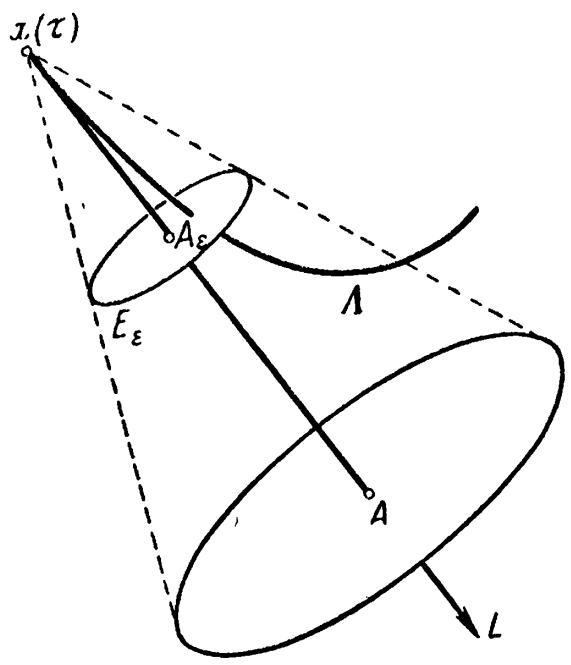
\includegraphics[max width=0.5\textwidth]{images/bo_d547imjef24c73bgfcdg_107_104_1256_571_665_0.jpg}
\end{center}
\hspace*{3em}

Prac. 31.

Так как в нашем рассужде- нии рассматриваются лишь та- кие символы а, которые являются линейными комбина- циями (с неотрицательными коэффициентами) к о н е ч- н о г о числа символов а, а, а, и, i, i = 1, 2,..., n, то точки \({\tau }_{j},{v}_{j},j = 1,2,\ldots,s\), входящие в определение символа а \(= \mathfrak{a}\left( {{\rho }^{1},\ldots,{\rho }^{n}}\right)\),одинаковы для всех этих симво- лов, т. е. не зависят от \({\rho }^{1},\ldots,{\rho }^{n}\) ; точка т также фиксиро- вана. Числа же \(\delta {t}_{1},\ldots,\delta {t}_{s}\) и бі (определяющие проварьи- рованное управление и * (t)) зависят, причем непрерывно, от \({\rho }^{1},\ldots,{\rho }^{n}\). Поэтому мы будем писать и а би, чтобы подчеркнуть зависимость величин и* (t) и δt от ρ1, …, ρ". Траекторию \({x}^{ * }\left( t\right)\), исходящую из точки х, и соответст- вующую управлению \({u}^{ * }\left( t\right),6\) удем обозначать через \({x}_{\mathfrak{a}}^{ * }\left( t\right)\), так что соотношение (21) (в котором ξ0 = 0, ибо начальная точка совпадает с \({x}_{0}\) при всех ε) даст нам

\[
{x}_{a}^{ * }\left( {\tau  + {\varepsilon \delta }{t}_{a}}\right)  = x\left( \tau \right)  + {\varepsilon \Delta }{x}_{a} + o\left( \varepsilon \right) . \tag{31}
\]

Отметим, что траектория \({x}_{a}^{ * }\left( t\right)\) не преры в н о зависит от параметров \({\rho }^{1},\ldots,{\rho }^{n}\) ; точно так же число б \({t}_{\mathfrak{a}}\) н e- \({\pi p}\) e \(p\) ы в н о зависит от \({\rho }^{1},\ldots,{\rho }^{n}\). Поэтому и точка \({x}_{a}^{ * }\left( {\tau  + {\varepsilon \delta }{t}_{a}}\right)\) н e- \(\Pi\) p e p ы в н о зависит от \({\rho }^{1},\ldots,{\rho }^{n}\), а величина о (e) имеет равномерно по \({\rho }^{1},\ldots,{\rho }^{n}\) более высокий порядок малости, чем ε (см. замечание на стр. 103). Следовательно, когда точка (ρ',..., ρ') описывает шар (30), точка (31) пробегает (при любом фиксированном е) некоторый «диск» \({F}_{\varepsilon }\) (т. е. непрерывный образ шара (30); этот диск может иметь самопересечения и т. п.). С точ- ностью до малых более высокого порядка, чем ε, диск F, «совпадает» с шаром Ев (см. (31)); точнее говоря, точки диска \({F}_{\mathrm{\varepsilon }}\) отстоят от соответствующих точек шара \({E}_{\mathrm{\varepsilon }}\) на величину более высокого порядка малости, чем ε (равномерно для всех точек шара \({E}_{\varepsilon }\) ). Точка же пере- сечения этого шара с линией Л (существующая при доста- точно малых ε) отстоит от точки х (т) и от границы шара \({E}_{\varepsilon }\) на величину порядка ε. Следовательно, при достаточно малом ε диск F в п е р е с е к а е т линию Λ в некоторой точке *) (рис. 32). Выберем такое ε. Так как весь диск \({F}_{\varepsilon }\) состоит из точек вида (31), то доказанный факт пересечения \({F}_{\varepsilon }\) c линией \(\Lambda\) означает: существуют такие \({\rho }^{1},\ldots,{\rho }^{n}\) (лежащие в шаре (30)), что \({x}_{\mathfrak{a}}^{ * }\left( {\tau  + {\varepsilon \delta }{t}_{\mathfrak{a}}}\right)  \in  \Lambda\). Иначе говоря, обозначив величины \({u}_{\mathfrak{a}}^{ * }\left( t\right),{x}_{\mathfrak{a}}^{ * }\left( t\right),{x}_{\mathfrak{a}}^{ * }\left( t\right)\), соответ- ствующие выбранным значениям \({\rho }^{1},\ldots,{\rho }^{n}\),через \({u}_{ * }\left( t\right)\), \({x}_{ * }\left( t\right)\) u полагая \(\tau  + {\varepsilon \delta }{t}_{a} = {\tau }^{\prime }\),мы получим \({x}_{ * }\left( {t}_{0}\right)  = {x}_{0}\), \({x}_{ * }\left( {\tau }^{\prime }\right)  \in  \Lambda\),и лемма 3 доказана.

\begin{center}
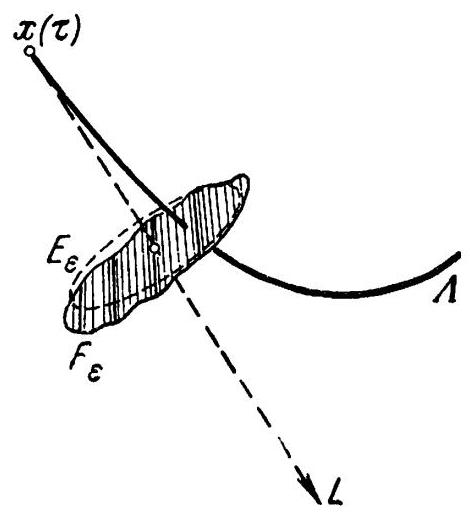
\includegraphics[max width=0.4\textwidth]{images/bo_d547imjef24c73bgfcdg_108_948_942_470_516_0.jpg}
\end{center}
\hspace*{3em}

Puc. 32.

\HRule

*) Факт существования такой точки пересечения представляется наглядно «очевидным»; строгое доказательство легко проводится элементарными средствами т о п о л о г и и (с помощью понятия

\HRule

Л е м м а 4. Если управление и (t) и соответствующая ему траектория \(x\left( t\right),{t}_{0} \leq  t \leq  {t}_{1}\), оптимальны, mo для любой правильной точки τ ( t, < τ < t, луч L, т, исходящий из точки х (т) и идущий в направлении отрицательной полуоси х \({}^{0}\), не принадлежит внутренности конуса Кτ (т. е. проходит либо вне этого конуса, либо по его границе).

Доказательство. Допустим, что при некотором т луч L. принадлежит внутренности конуса K,. Применим лемму 3, принимая за линию \(\Lambda\) (и за луч L) луч L. Тогда мы получим, что существует такое управление \({u}_{ * }\left( t\right)\),для которого соответствующая траектория \({x}_{ * }\left( t\right)\) (исходящая из той же точки \({x}_{0}\) ) проходит в некоторый момент \({\tau }^{\prime } > {t}_{0}\) через точку,лежапую на луче \({L}_{\tau }\). Иначе говоря,

\[
{x}_{ * }^{i}\left( {\tau }^{\prime }\right)  = {x}^{i}\left( \tau \right) ,\;i = 1,2,\ldots ,n;
\]

\[
{x}_{ * }^{0}\left( {\tau }^{\prime }\right)  < {x}^{0}\left( \tau \right)
\]

Определим на отрезке \({t}_{0} \leq  t \leq  {t}_{1} + \left( {{\tau }^{\prime } - \tau }\right)\) управление \({u}_{* * }\left( t\right),\) положив

\[
{u}_{* * }\left( t\right)  = \left\{  \begin{array}{ll} {u}_{ * }\left( t\right) & \text{ при }{t}_{0} \leq  t \leq  {\tau }^{\prime }, \\  u\left( {t - \left( {{\tau }^{\prime } - \tau }\right) }\right) & \text{ при }{\tau }^{\prime } < t \leq  {t}_{1} + \left( {{\tau }^{\prime } - \tau }\right) . \end{array}\right.
\]

Траектория \({x}_{* * }\left( t\right)\), соответствующая управлению \({u}_{* * }\left( t\right)\) и исходящая из точки х, оховпадает, очевидно, на отрезке \({t}_{0} \leq  t \leq  {\tau }^{\prime }\) c траекторией \({x}_{ * }\left( t\right)\), rax что,в частности

(32)
\[
{x}_{* * }^{i}\left( {\tau }^{\prime }\right)  = {x}^{i}\left( \tau \right) ,\;i = 1,2,\ldots ,n;
\]

\[
{x}_{* * }^{0}\left( {\tau }^{\prime }\right)  < {x}^{0}\left( \tau \right)
\]

\HRule

индекса пересечения; см., например, В. Г. Б о д т т я н с к и й. топическая теория непрерывных отображений и векторных полей, Труды Матем. института им. В. А. Стеклова, т. XLVII, 1955; опре- деление индекса пересечения «отображенных», т. е. искривленных цепей дано в п. 5:2 этой книги, а существование при достаточно малом 8 точки пересечения диска F, и линии Л вытекает из предложения (r) на стр. 69).

\HRule

Далее,на отрезке \({\tau }^{\prime } \leq  t \leq  {t}_{1} + \left( {{\tau }^{\prime } - \tau }\right)\) траектория \({x}_{* * }\left( t\right)\) имеет вид

\[
{x}_{* * }\left( t\right)  = x\left( {t - \left( {{\tau }^{\prime } - \tau }\right) }\right)  + p, \tag{33}
\]

где p — постоянный вектор

\[
\mathbf{p} = \left( {{x}_{* * }^{0}\left( {\tau }^{\prime }\right)  - {x}^{0}\left( \tau \right) ,0,0,\ldots ,0}\right) .
\]

(Это получается непосредственной подстановкой реше- ния (33) в уравнения (7) с учетом того факта, что правые части системы (7) не зависят от t и x0; вектор p опре- деляется тем условием, что в точке で точке «стыка» двух кусков траектории \({x}_{* * }\left( t\right)\) — эта траектория должна быть непрерывна.) При \(t = {t}_{1} + \left( {{\tau }^{\prime } - \tau }\right)\) получаем

\[
{x}_{* * }\left( {{t}_{1} + \left( {{\tau }^{\prime } - \tau }\right) }\right)  = x\left( {t}_{1}\right)  + p.
\]

Иначе говоря, точка \({x}_{* * }\left( {{t}_{1} + \left( {{\tau }^{\prime } - \tau }\right) }\right)\) лежит на прямой П, определенной в \$ 11 (ибо вектор p параллелен оси и’), и, кроме того,

\[
{x}_{* * }^{0}\left( {{t}_{1} + \left( {{\tau }^{\prime } - \tau }\right) }\right)  = {x}^{0}\left( {t}_{1}\right)  + {x}_{* * }^{0}\left( {\tau }^{\prime }\right)  - {x}^{0}\left( \tau \right)  < {x}^{0}\left( {t}_{1}\right)
\]

(см. (32)). Но это противоречит оптимальности траекто- рии х (t) и управления и (t). Таким образом, предположе- ние, сделанное в начале доказательства, приводит к про- тиворечию, и лемма 4 полностью доказана.

\section*{§ 15. Доказательство принципа максимума}

B этом параграфе мы будем предполагать, что х (t), \({t}_{0} \leq  t \leq  {t}_{1}\),—оптимальная траектория (соединяющая точку \({x}_{0}\) c некоторой точкой прямой \(\Pi\),см. § 11), a \(u\left( t\right)\) — соответ- ствующее оптимальное управление. Пусть τ — некоторая правильная точка управления и (t). Согласно лемме 4, луч L. не принадлежит внутренности конуса K, так что этот конус не заполняет всего пространства Х. Поэтому существует опорная гиперплоскость к конусу K, в его верппине, т. е. такая гиперплоскость \(\Gamma\), что весь конус \({K}_{\text{ : }}\) лежит в одном из двух замкнутых полупространств, опре- деляемых гиперплоскостью Г. (Гиперплоскость Г, обла- дающая этим свойством, может быть не единственной; последующие рассуждения справедливы для любой такой гиперплоскости.) Уравнение гиперплоскости Г (в прост- ранстве X,) можно записать в виде \(\mathop{\sum }\limits_{{\alpha  = 0}}^{n}{a}_{\alpha }{x}^{\alpha } = 0\),где \({x}^{0},{x}^{1},\ldots,{x}^{n}\) - текущие координаты. Так как умножение всех коэффициентов \({a}_{\alpha }\) на одно и то же отличное от нуля число не меняет гиперплоскости \(\Gamma\),то мы можем считать (изменив, если нужно, знаки всех чисел а а на обратные), что конус \({K}_{\tau }\) лежит в о т р и ц и а т е л ь н о м полупрост- ранстве \(\left( {\mathop{\sum }\limits_{{\alpha  = 0}}^{n}{a}_{\alpha }{x}^{\alpha } \leq  0}\right)\). Иначе говоря, для любого вектора \({\Delta x}\), определяемого формулой (22),выполнено неравенство

\[
\left( {a,{\Delta x}}\right)  \leq  0\;\left( {{\Delta x} \in  {K}_{\tau }}\right) , \tag{34}
\]

где через а обозначен вектор \(\left( {{a}_{0},{a}_{1},\ldots,{a}_{n}}\right)\) (ибо сово- купность векторов (22) и есть конус K,). Полагая в фор- муле (22) \(\delta {t}_{1} = \delta {t}_{2} = \ldots  = \delta {t}_{s} = 0\),мы получим \({\Delta x} = \; = f\left( {x\left( \tau \right),u\left( \tau \right) }\right) {\delta t},u,\) в салу (34),

\[
\left( {a,f\left( {x\left( \tau \right) ,u\left( \tau \right) }\right) {\delta t}}\right)  \leq  0.
\]

Так как это неравенство справедливо при любых би (как положительных, так и отрицательных), то

\[
\left( {a,f\left( {x\left( \tau \right) ,u\left( \tau \right) }\right) }\right)  = 0,
\]

т. е., иначе говоря,

\[
\mathcal{K}\left( {a,x\left( \tau \right) ,u\left( \tau \right) }\right)  = 0 \tag{35}
\]

(это соотношение выполняется, если вектор а удовлетво- ряет условию (34)). Обозначим через

\[
\psi \left( {t,a}\right)  = \left( {{\psi }_{0}\left( {t,a}\right) ,{\psi }_{1}\left( {t,a}\right) ,\ldots ,{\psi }_{n}\left( {t,a}\right) }\right)
\]

решение системы уравнений (8) (соответствующее изучае- мым оптимальным и (t) и x (t)) с начальным условием

\[
\psi \left( {\tau ,a}\right)  = a. \tag{36}
\]

Решение ψ \(\left( {t,a}\right)\) определено на всем отрезке \({t}_{0} \leq  t \leq  {t}_{1}\), так как система (8) линейна.

Л е м м а 5. Если вектор а удовлетворяет условию (34), то во всякой правильной точке управления и (t), лежащей на полуинтервале \({t}_{0} < t \leq  \tau\), выполнено соотношение

\[
\mathcal{K}\left( {\psi \left( {t,a}\right) ,x\left( t\right) ,u\left( t\right) }\right)  = \mathcal{M}\left( {\psi \left( {t,a}\right) ,x\left( t\right) }\right) .
\]

Пусть ти правильная точка управления \(u\left( t\right)\), расположен- ная на полуинтервале \({t}_{0} < t \leq  \tau\), a \({v}_{1} -\) произвольная точка пространства U. Рассмотрим символ а (см. § 14) с един- ственной точкой \({\tau }_{1}\) (т. e. \(s = 1\) ) и с числами \(\delta {t}_{1},{\delta t}\), coor- ветственно равными единице и нулю:

\[
a = \left\{  {{\tau }_{1},{v}_{1},\tau ,1,0}\right\}  .
\]

Тогда вектор \({\Delta x}\) (см. 22)), соответствующий этому сим- волу а, будет иметь значение

\[
{\Delta x} = {A}_{\tau ,{\tau }_{1}}\left\lbrack  {f\left( {x\left( {\tau }_{1}\right) ,{v}_{1}}\right)  - f\left( {x\left( {\tau }_{1}\right) ,u\left( {\tau }_{1}\right) }\right) }\right\rbrack  .
\]

B силу соотношений (34) и (36) получаем отсюда

\[
\left( {\psi \left( {\tau ,a}\right) ,{A}_{\tau ,{\tau }_{1}}\left\lbrack  {f\left( {x\left( {\tau }_{1}\right) ,{v}_{1}}\right)  - f\left( {x\left( {\tau }_{1}\right) ,u\left( {\tau }_{1}\right) }\right) }\right\rbrack  }\right)  \leq  0,
\]

и потому, согласно лемме 1 и соотношению \({A}_{{\tau }_{1},{\tau }_{1}} = E\) (см. (17))

\[
\left( {\psi \left( {{\tau }_{1},a}\right) ,f\left( {x\left( {\tau }_{1}\right) ,{v}_{1}}\right)  - f\left( {x\left( {\tau }_{1}\right) ,u\left( {\tau }_{1}\right) }\right) }\right)  \leq  0.
\]

Это соотношение переписывается (в силу определения функции \(\mathcal{K}\) ) в виде

\[
\mathcal{K}\left( {\psi \left( {{\tau }_{1},a}\right) ,x\left( {\tau }_{1}\right) ,{v}_{1}}\right)  - \mathcal{K}\left( {\psi \left( {{\tau }_{1},a}\right) ,x\left( {\tau }_{1}\right) ,u\left( {\tau }_{1}\right) }\right)  \leq  0,
\]

а так как это неравенство справедливо для любой точки \({v}_{1} \in  U\), то мы получаем

\[
\mathcal{K}\left( {\psi \left( {{\tau }_{1},a}\right) ,x\left( {\tau }_{1}\right) ,u\left( {\tau }_{1}\right) }\right)  = \mathop{\max }\limits_{{{v}_{1} \in  U}}\mathcal{K}\left( {\psi \left( {{\tau }_{1},a}\right) ,x\left( {\tau }_{1}\right) ,{v}_{1}}\right)  =
\]

\[
= \mathcal{M}\left( {\psi \left( {{\tau }_{1},a}\right) ,x\left( {\tau }_{1}\right) }\right) ,
\]

и лемма 5 доказана.

Соотношение, указанное в лемме 5, справедливо и при \(t = \tau\) (ибо т правильная точка):

\[
\mathcal{K}\left( {\psi \left( {\tau ,a}\right) ,x\left( \tau \right) ,u\left( \tau \right) }\right)  = \mathcal{M}\left( {\psi \left( {\tau ,a}\right) ,x\left( \tau \right) }\right) .
\]

Поэтому, в силу (35) и (36), мы получаем следующее утверждение.

Ле мм а 6. Если вектор а удовлетворяет условию (34), mo

\[
\mathcal{M}\left( {\psi \left( {\tau ,a}\right) ,x\left( \tau \right) }\right)  = 0.
\]

Л е м м а 7. Если абсолютно непрерывная функция ψ (t) почти всюду на некотором отрезке I удовлетворяет уравне- ниям (8) и соотношению

\[
\mathcal{K}\left( {\psi \left( t\right) ,x\left( t\right) ,u\left( t\right) }\right)  = \mathcal{M}\left( {\psi \left( t\right) ,x\left( t\right) }\right) , \tag{37}
\]

то функция \(\mathcal{M}\left( {\psi \left( t\right),x\left( t\right) }\right)\) постоянна на всем отрезке I.

Заметим прежде всего, что функция \(\mathcal{M}\left( {\psi \left( t\right),x\left( t\right) }\right)\) полунепрерывна снизу на отрезке I. Действительно, пусть \({t}^{\prime }\) — произвольная точка этого отрезка, а ε — положитель- ное число. В силу определения верхней грани, существует такая точка \({u}^{\prime } \in  U\),что

\[
\mathcal{K}\left( {\psi \left( {t}^{\prime }\right) ,x\left( {t}^{\prime }\right) ,{u}^{\prime }}\right)  \geq  \mathcal{M}\left( {\psi \left( {t}^{\prime }\right) ,x\left( {t}^{\prime }\right) }\right)  - \frac{\varepsilon }{2}.
\]

Далее, в силу непрерывности функции \(\mathcal{K}\left( {\psi \left( t\right),x\left( t\right),u}\right)\) по \(t\) при фиксированном \(u = {u}^{\prime }\), существует такое \(\delta  > 0\), что при | \(t - {t}^{\prime } \mid   < \delta\) имеем

\[
\left| {\mathcal{K}\left( {\psi \left( t\right) ,x\left( t\right) ,{u}^{\prime }}\right)  - \mathcal{K}\left( {\psi \left( {t}^{\prime }\right) ,x\left( {t}^{\prime }\right) ,{u}^{\prime }}\right) }\right|  < \frac{\varepsilon }{2}.
\]

Таким образом,при \(\left| {t - {t}^{\prime }}\right|  < \delta\) справедливо неравенство

\[
\mathcal{M}\left( {\psi \left( t\right) ,x\left( t\right) }\right)  = \mathop{\sup }\limits_{{u \in  U}}\mathcal{K}\left( {\psi \left( t\right) ,x\left( t\right) ,u}\right)  \geq
\]

\[
\geq  \mathcal{K}\left( {\psi \left( t\right) ,x\left( t\right) ,{u}^{\prime }}\right)  > \mathcal{M}\left( {\psi \left( {t}^{\prime }\right) ,x\left( {t}^{\prime }\right) }\right)  - \varepsilon ,
\]

показывающее, что функция \(\mathcal{M}\left( {\psi \left( t\right),x\left( t\right) }\right)\) полунепре- рывна снизу.

Далее, так как управление и (t) допустимо, то образ отрезка \(I\) при отображении \(u\) обладает в пространстве \({E}_{r}\) компактным замыканием (см. § 10), т. е. существует в \({E}_{r}\) такое компактное множество \(P\),что \(u\left( t\right)  \in  P\) при \(t \in  I\). Положим

\[
m\left( {\psi ,x}\right)  = \mathop{\max }\limits_{{u \in  P}}\mathcal{K}\left( {\psi ,x,u}\right) .
\]

Очевидно, что имеет место неравенство

\[
\mathcal{M}\left( {\psi ,x}\right)  \geq  m\left( {\psi ,x}\right) , \tag{38}
\]

справедливое при любых х и Ф. Соотношение (37) озна- чает, что почти всюду на отрезке I имеет место равенство

\[
m\left( {\psi \left( t\right) ,x\left( t\right) }\right)  = \mathcal{M}\left( {\psi \left( t\right) ,x\left( t\right) }\right)
\]

(πбо \(u\left( t\right)  \in  P\) ).

Итак, \(\mathcal{M}\left( {\psi \left( t\right),x\left( t\right) }\right)\) есть полунепрерывная снизу функ- ция, почти всюду на отрезке I совпадающая с функцией \(m\left( {\psi \left( t\right),x\left( t\right) }\right)\) и связанная с ней соотношением (38). Из этого следует, что если функция \(m\left( {\psi \left( t\right),x\left( t\right) }\right)\) непре- рывна, то функция М (ψ (t), x (t)) в с юд у на отрезке I совпадает с ней (и потому также непрерывна). Мы сейчас покажем, что функция \(m\left( {\psi \left( t\right),x\left( t\right) }\right)\),— а следовательно, в силу сказанного, и м Ж (ψ (t), x (t)),— а б с о л ю т н о не п р е р ы в н а на отрезке I.

Так как отрезок I компактен, то существует в про- странстве переменных \({\psi }_{0},{\psi }_{1},\ldots,{\psi }_{n},{x}^{0},{x}^{1},\ldots,{x}^{n}\) такое выпуклое ограниченное множество Q, что точка \(\left( {\psi \left( t\right),x\left( t\right) }\right)\) принадлежит множеству \(Q\) при \(t \in  I\). Таким образом, тройка (ψ (t), x (t)) принадлежит множеству \(Q \times  P\) при \(t \in  I\). Далее, так как частные производные функ- ции \(\mathcal{K}\left( {\psi,x,u}\right)\) по переменным \({\psi }_{\alpha },{x}^{\alpha }\),непрерывны по сово- купности переменных ψ, х, и (см. условия, наложенные на функции \({f}^{i}\) в § 11), то на компактном множестве Q×P все эти производные ограничены. Отсюда следует сущест- вование такой (не зависящей от и) константы \(K > 0\),что для любых (ψ, x) \(\in  Q,\left( {{\psi }^{\prime },{x}^{\prime }}\right)  \in  Q,u \in  P\) выполнено соотношение

\[
\left| {\mathcal{K}\left( {\psi ,x,u}\right)  - \mathcal{K}\left( {{\psi }^{\prime },{x}^{\prime },u}\right) }\right|  \leq  {Kd}, \tag{39}
\]

где d — наибольшее из чисел \(\left| {{\psi }_{i} - {\psi }_{i}^{\prime }}\right|\), \(\left| {{x}^{i} - {x}^{\prime i}}\right|\), \(i = 0,1,\ldots,n.\) Пусть (ψ, x) и ( \({\psi }^{\prime },{x}^{\prime }\) ) — две точки множе- ства Q, а и и \({u}^{\prime }\) — такие точки множества P, что

\[
m\left( {\psi ,x}\right)  = \mathcal{K}\left( {\psi ,x,u}\right) ,m\left( {{\psi }^{\prime },{x}^{\prime }}\right)  = \mathcal{K}\left( {{\psi }^{\prime },{x}^{\prime },{u}^{\prime }}\right) .
\]

Тогда, очевидно, выполнены неравенства

\[
\mathcal{K}\left( {\psi ,x,{u}^{\prime }}\right)  \leq  \mathcal{K}\left( {\psi ,x,u}\right) ,\mathcal{K}\left( {{\psi }^{\prime },{x}^{\prime },u}\right)  \leq  \mathcal{K}\left( {{\psi }^{\prime },{x}^{\prime },{u}^{\prime }}\right) ,
\]

и потому (учитывая соотношение (39)) мы получаем

\[
- {Kd} \leq  \mathcal{K}\left( {\psi ,x,{u}^{\prime }}\right)  - \mathcal{K}\left( {{\psi }^{\prime },{x}^{\prime },{u}^{\prime }}\right)  \leq
\]

\[
\leq  \mathcal{K}\left( {\psi ,x,u}\right)  - \mathcal{K}\left( {{\psi }^{\prime },{x}^{\prime },{u}^{\prime }}\right)  \leq
\]

\[
\leq  \mathcal{K}\left( {\psi ,x,u}\right)  - \mathcal{K}\left( {{\psi }^{\prime },{x}^{\prime },{u}^{\prime }}\right)  \leq  {Kd}.
\]

Иначе говоря,

\[
\left| {m\left( {\psi ,x}\right)  - m\left( {{\psi }^{\prime },{x}^{\prime }}\right) }\right|  \leq  {Kd}
\]

где d — наибольшее из чисел | ̸ \({\psi }_{i}\) — у т е те ть не зере не не не при кере пределеннег \(i = 0,1,\ldots,n\). B частности, отсюда получаем

\[
\left| {m\left( {\psi \left( t\right) ,x\left( t\right) }\right)  - m\left( {\psi \left( {t}^{\prime }\right) ,x\left( {t}^{\prime }\right) }\right) }\right|  \leq  {Kd},t,{t}^{\prime } \in  I,
\]

где \(d\) - наибольшее из чисел \(\left| {{\psi }_{i}\left( t\right)  - {\psi }_{i}\left( {t}^{\prime }\right) }\right|,\left| {{x}^{i}\left( t\right)  - {x}^{i}\left( {t}^{\prime }\right) }\right|\). Из этого неравенства, в силу абсолютной непрерывности функций \(\psi \left( t\right)\) и \(x\left( t\right)\),мы без труда заключаем,что функ- ция \(m\left( {\psi \left( t\right),x\left( t\right) }\right)\) абсолютно непрерывна.

Покажем, наконец, что функция \(m\left( {\psi \left( t\right),x\left( t\right) }\right)\) почти всюду имеет производную, равную нулю. В силу абсо- лютной непрерывности функции \(m\left( {\psi \left( t\right),x\left( t\right) }\right)\) и опреде- ления функций \(x\left( t\right)\) и \(\psi \left( t\right)\),почти всюду на отрезке I имеют место следующие обстоятельства: функция \(m\left( {\psi \left( t\right),x\left( t\right) }\right)\) имеет производную, для функций х (t) и ψ (t) выпол- нены соотношения (7) и (8), или, что то же самое, (9) и (10), и, кроме того,

\[
m\left( {\psi \left( t\right) ,x\left( t\right) }\right)  = \mathcal{K}\left( {\psi \left( t\right) ,x\left( t\right) ,u\left( t\right) }\right) .
\]

Пусть \(t = \tau  -\) какая-либо точка, в которой эти обстоятель- ства имеют место, и т’ — произвольная отличная от τ точка отрезка I. Тогда

\[
m\left( {\psi \left( {t}^{\prime }\right) ,x\left( {t}^{\prime }\right) }\right)  \geq  \mathcal{K}\left( {\psi \left( {t}^{\prime }\right) ,x\left( {t}^{\prime }\right) ,u\left( \tau \right) }\right)
\]

II IIOTOMY

\[
m\left( {\psi \left( {t}^{\prime }\right) ,x\left( {t}^{\prime }\right) }\right)  - m\left( {\psi \left( \tau \right) ,x\left( \tau \right) }\right)  \geq
\]

\[
\geq  \mathcal{K}\left( {\psi \left( {t}^{\prime }\right) ,x\left( {t}^{\prime }\right) ,u\left( \tau \right) }\right)  - \mathcal{K}\left( {\psi \left( \tau \right) ,x\left( \tau \right) ,u\left( \tau \right) }\right) .
\]

Будем теперь считать, что ти приближается к т, оста- ваясь больше т, так что разность \({t}^{\prime } - \tau\) положительна. Тогда деление на t’ — т не меняет знака неравенства в последнем соотношении:

\[
\frac{m\left( {\psi \left( {t}^{\prime }\right) ,x\left( {t}^{\prime }\right) }\right)  - m\left( {\psi \left( \tau \right) ,x\left( \tau \right) }\right) }{{t}^{\prime } - \tau } \geq
\]

\[
\geq  \frac{\mathcal{K}\left( {\psi \left( {t}^{\prime }\right) ,x\left( {t}^{\prime }\right) ,u\left( \tau \right) }\right)  - \mathcal{K}\left( {\psi \left( \tau \right) ,x\left( \tau \right) ,u\left( \tau \right) }\right) }{{t}^{\prime } - \tau }.
\]

Переходя к пределу при \({t}^{\prime } \rightarrow  \tau \left( {{t}^{\prime } > \tau }\right)\),получаем отсюда

\[
{\left. \frac{d}{dt}m\left( \psi \left( t\right) ,x\left( t\right) \right) \right| }_{t = \tau } = {\left. \frac{d}{dt}\mathcal{K}\left( \psi \left( t\right) ,x\left( t\right) ,u\left( \tau \right) \right) \right| }_{t = \tau } =
\]

\[
= {\left. \mathop{\sum }\limits_{{\alpha  = 0}}^{n}\frac{\partial \mathcal{H}}{\partial {\psi }_{\alpha }} \cdot  \frac{d{\psi }_{\alpha }\left( t\right) }{dt}\right| }_{t = \tau } + {\left. \mathop{\sum }\limits_{{\alpha  = 0}}^{n}\frac{\partial \mathcal{H}}{\partial {x}^{\alpha }} \cdot  \frac{d{x}^{\alpha }\left( t\right) }{dt}\right| }_{t = \tau } = 0
\]

(здесь производные вычисляются в точке τ, где τ и, следо- вательно, \(u\left( \tau \right)\) фиксированы). Аналогично, при \({t}^{\prime } \rightarrow  \tau\), \({t}^{\prime } < \tau\) получаем обратное неравенство

\[
{\left. \frac{d}{dt}m\left( \psi \left( t\right) ,x\left( t\right) \right) \right| }_{t = \tau } \leq  0.
\]

Итак, \(m\left( {\psi \left( t\right),x\left( t\right) }\right)\), a также и совпадающая с ней функция М (ф (н), х (t)), есть абсолютно непрерывная функ- ция, имеющая почти всюду производную, равную нулю. Следовательно, эта функция постоянна на отрезке I.

Докажем следующее важное свойство конусов Кт.

JI e м м а 8. Если τ и τ’ — правильные точки управле- ния \(u\left( t\right)\), причем \({t}_{0} < {\tau }^{\prime } < \tau  < {t}_{1}\), mo \({A}_{\tau,{\tau }^{\prime }}\left( {K}_{{\tau }^{\prime }}\right)  \subset  {K}_{\tau }\), еде \({A}_{\tau,{\tau }^{\prime }}\) - отображение пространства Х \({}_{{\tau }^{\prime }}\) на \({X}_{\tau }\), on ределен- ное в \$ 12.

B самом деле, конус ку образован векторами, каждый из которых в силу (22) можно представить в виде суммы двух векторов: \({\Delta }_{1}x = f\left( {x\left( {\tau }^{\prime }\right),u\left( {\tau }^{\prime }\right) }\right) {\delta t}\),

\[
{\Delta }_{2}x = \mathop{\sum }\limits_{{i = 1}}^{s}{A}_{{\tau }^{\prime },{\tau }_{i}}\left\lbrack  {f\left( {x\left( {\tau }_{i}\right) ,{v}_{i}}\right)  - f\left( {x\left( {\tau }_{i}\right) ,u\left( {\tau }_{i}\right) }\right) }\right\rbrack  \delta {t}_{i}.
\]

Поэтому достаточно показать, что имеют место включения

\[
{A}_{\tau ,{\tau }^{\prime }}\left( {{\Delta }_{1}x}\right)  \in  {K}_{\tau },\;{A}_{\tau ,{\tau }^{\prime }}\left( {{\Delta }_{2}x}\right)  \in  {K}_{\tau }. \tag{40}
\]

Мы имеем в силу (17):

\[
{A}_{\tau ,{\tau }^{\prime }}\left( {{\Delta }_{2}x}\right)  = \mathop{\sum }\limits_{{i = 1}}^{8}{A}_{\tau ,{\tau }_{i}}\left\lbrack  {f\left( {x\left( {\tau }_{i}\right) ,{v}_{i}}\right)  - f\left( {x\left( {\tau }_{i}\right) ,u\left( {\tau }_{i}\right) }\right) }\right\rbrack  \delta {t}_{i},
\]

и потому второе из включений (40) имеет место (ибо \({\tau }_{1} \leq  \ldots  \leq  {\tau }_{s} \leq  {\tau }^{\prime } < \tau )\). Докажем первое из этих включений. Допустим, что (при некотором \({\delta t}\) ) вектор \({A}_{\tau,{\tau }^{\prime }}\left( {{\Delta }_{1}x}\right)\) не при- надлежит конусу K,- Тогда существует гиперплоскость, разделяющая их, т. е. существуют такие числа а, а, и,..., а, что конус Kτ расположен в отрицательном полупростран-

CTBe \(\mathop{\sum }\limits_{{\alpha  = 0}}^{n}{a}_{\alpha }{x}^{\alpha } \leq  0\), a вектор \({A}_{\tau,{\tau }^{\prime }}\left( {{\Delta }_{1}x}\right)  - B\) 0 ТКры T0 M положительном полупространстве, т. е.

\[
\left( {\mathbf{a},{A}_{\tau ,{\tau }^{\prime }}\left( {{\Delta }_{1}\mathbf{x}}\right) }\right)  > 0, \tag{41}
\]

где a — вектор \(\left( {{a}_{0},{a}_{1},\ldots,{a}_{n}}\right)\). Обозначим через ψ (t, a) реше- ние системы (8) с начальным условием ψ (τ, α) = a. Это решение мы будем рассматривать на отрезке \({t}_{0} \leq  t \leq  \tau\). Так как конус K т расположен в отрицательном полупростран- стве, т. е. выполнено условие (34), то из лемм 5, 7 и 6 вытекает, что М \(\left( {\psi \left( {t,a}\right),x\left( t\right) }\right)  \equiv  0\) при \({t}_{0} \leq  t \leq  \tau\). Tak как, далее, т’ — правильная точка (лежащая на полуинтер- вале \({t}_{0} < t \leq  \tau\) ), то, согласно лемме 5,

\[
\mathcal{M}\left( {\psi \left( {{\tau }^{\prime },a}\right) ,x\left( {\tau }^{\prime }\right) ,u\left( {\tau }^{\prime }\right) }\right)  = \mathcal{M}\left( {\psi \left( {{\tau }^{\prime },a}\right) ,x\left( {\tau }^{\prime }\right) }\right)  = 0,
\]

T. e.

\[
\left( {\psi \left( {{\tau }^{\prime },a}\right) ,f\left( {x\left( {\tau }^{\prime }\right) ,u\left( {\tau }^{\prime }\right) }\right) }\right)  = 0.
\]

Отсюда, согласно лемме 1, мы получаем соотношение

\[
\left( {\psi \left( {\tau ,a}\right) ,{A}_{\tau ,{\tau }^{\prime }}\left( {f\left( {x\left( {\tau }^{\prime }\right) ,u\left( {\tau }^{\prime }\right) }\right) }\right)  = 0,}\right.
\]

противоречапее неравенству (41). Полученное противоре- чие и доказывает лемму 8.

Пусть теперь \(\tau\) -произвольная правильная точка упра- вления \(u\left( t\right)\),лежапая на интервале \({t}_{0} < t < {t}_{1}\). Положим \({K}_{{t}_{1}}^{\left( \tau \right) } = {A}_{{t}_{1},\tau }\left( {K}_{\tau }\right)\). Tak rax \({A}_{{t}_{1},\tau }\) ects линейное отображе- ние,то \({K}_{{t}_{1}}^{\left( \tau \right) }\) есть выпуклыйконус пространства \({X}_{{t}_{1}}\).Кону- сы \({K}_{{t}_{1}}^{\left( \tau \right) }\) образуют в о 3 p a c r a ю m у ю п о c л e д o в a- т е л ь н о c т ь: если т’ с т правильные точки, то в силу леммы 8 мы имеем (см. (17))

\[
{K}_{{t}_{1}}^{\left( {\tau }^{\prime }\right) } = {A}_{{t}_{1},{\tau }^{\prime }}\left( {K}_{{\tau }^{\prime }}\right)  = {A}_{{t}_{1},\tau }\left( {{A}_{\tau ,{\tau }^{\prime }}\left( {K}_{{\tau }^{\prime }}\right) }\right)  \subset  {A}_{{t}_{1},\tau }\left( {K}_{\tau }\right)  = {K}_{{t}_{1}}^{\left( \tau \right) }.
\]

Поэтому объединение (по всем правильным точкам τ интер- вала \({t}_{0} < t < {t}_{1}\) ) всех конусов K, \({}^{\left( \tau \right) }\) chosa есть выпуклый конус (возможно не замкнутый) пространства \({\mathbf{X}}_{{t}_{1}}\) (с вер- шиной в начале). Этот конус мы обозначим через к, и назовем предельным конусом.

JI e м м а 9. Если управление и (t) и соответствующая траектория \(x\left( t\right),{t}_{0} \leq  t \leq  {t}_{1}\), оптимальны, mo луч L \({L}_{{t}_{1}}\), исходящий из точки х (кі) в направлении отрицательной полуоси х0, не принадлежит внутренности конуса К1,.

В самом деле, пусть луч L, принадлежит внутрен- ности конуса Ки,. Выберем выпуклый многогранник M, целиком лежащий в Ки, и содержащий какую-либо точку \(l \in  {L}_{{t}_{1}}\) внутри себя. Каждая вершина многогранника \(M\) принадлежит конусу K, т. е. принадлежит некоторому конусу К \({t}_{1}^{\left( \tau \right) }\), a так как конусы Киз образуют возрастающую последовательность, то найдется такая правильная точка τ, что в с е вершины многогранника М принадлежат конусу \({K}_{{t}_{1}}^{\left( \tau \right) }\). Следовательно, конус Киси сей/с одержит весь многогранник \(M\),так что точка \(l\) является внутренней точкой конуса Ки; или, что то же самое, луч L, принадлежит внутренности конуса \({K}_{{t}_{1}}^{\left( \tau \right) }\). Ho тогда луч \({A}_{{t}_{1},\tau }^{-1}\left( {L}_{{t}_{1}}\right)\) принадлежит внут- ренности конуса \({A}_{{t}_{1},\tau }^{-1}\left( {K}_{{t}_{1}}^{\left( \tau \right) }\right)  = {K}_{\tau }\) (ибо \({A}_{{t}_{1},\tau }^{-1}\) есть линей- ное невырожденное, следовательно, гомеоморфное отобра- жение). Луч же \({A}_{{t}_{1},\tau }^{-1}\left( {L}_{{t}_{1}}\right)\) совпадает с лучом \({L}_{\tau }\),исходя- щим из точки х (т) в направлении отрицательной полуоси \({x}^{0}\). Это вытекает из того, что система уравнений в вариациях (16) не содержит в своих правых частях переменного и’, и потому равные между собой векторы ( — 1, 0, 0,...,0), исходящие из точек кривой \(x\left( t\right)\),получаются друг из друга переносом вдоль траектории \(x\left( t\right)\).

Итак, луч L т принадлежит внутренности конуса K, а это противоречит оптимальности управления и (t) (см. лемму 4).

Переходим к завершению доказательства теоремы 8. Пусть \(u\left( t\right),{t}_{0} \leq  t \leq  {t}_{1}\),— оптимальное управление, а х(t)— соответствующая ему оптимальная траектория. Тогда луч \({L}_{{t}_{1}}\) не принадлежит внутренности предельного конуса К \({t}_{{t}_{1}}\) (лемма 9), и потому существует разделяющая их гипер- плоскость, т. е. существуют такие числа с, с, п. с. п. р. пс. ра что весь конус \({K}_{{t}_{1}}\) лежит в полупространстве. \(\mathop{\sum }\limits_{n}^{n}{c}_{\alpha }{x}^{\alpha } \leq  0\), a луч L+ B полупространстве дел С 10 и 11 ее то 11 наче го- воря, вектор (-1, 0, 0,..., 0), имеющий направле- ние луча \({L}_{{t}_{1}}\),лежит в замкнутом полупространстве

\[
\mathop{\sum }\limits_{{\alpha  = 0}}^{n}{c}_{\alpha }{x}^{\alpha } \geq  0,\text{ т. е. }{c}_{0} \leq  0.
\]

Обозначим через ψ (t) = ( \({\psi }_{0}\left( t\right),{\psi }_{1}\left( t\right),\ldots,{\psi }_{n}\left( t\right)\) ) perme- ние системы (8) с начальным условием ψ (t) = c, где \(c\) - вектор \(\left( {{c}_{0},{c}_{1},\ldots,{c}_{n}}\right)\). Так как система (8) линейна, то решение \(\psi \left( t\right)\) определено на всем отрезке \({t}_{0} \leq  t \leq  {t}_{1}\). Покажем, что вектор ψ(t) и является тем вектором, существование которого утверждается в теореме 8.

Прежде всего, \(x\left( t\right)\) и \(\psi \left( t\right)\) удовлетворяют уравнениям (7) и (8), или, что то же самое, (9) и (10). Докажем, что соотношение (11) имеет место во всякой правильной точке интервала \({t}_{0} < t < {t}_{1}\). Пусть т правильная точка, лежащая на этом интервале. Так как весь конус Ки, а следовательно, и конус \({A}_{{t}_{1},\tau }\left( {K}_{\tau }\right)\) лежит в отрицатель- ном полупространстве дел \({\psi }_{\alpha }\left( {t}_{1}\right) {x}^{\alpha } \leq  0\), TO (совершая пере- нос вдоль траектории \(x\left( t\right)\) из точки x \(\left( {t}_{1}\right)\) в точку x (t) мы получаем,что весь конус \({A}_{{t}_{1},\tau }^{-1}\left( {{A}_{{t}_{1},\tau }\left( {K}_{\tau }\right) }\right)  = {K}_{\tau }\) лежит в полупространстве дел \({\psi }_{\alpha }\left( \tau \right) {x}^{\alpha } \leq  0\) (см. § 12). Иначе говоря, вектор \(a = \psi \left( \tau \right)\) удовлетворяет условию (34). Отсюда вытекает, что для решения ψ (t, a) уравнения (8) с начальным условием ψ (т, а) = a – a это решение, оче- видно, совпадает с ψ (t) — справедливо утверждение лем- мы 5. В частности (в силу того, что τ — правильная точка),

\[
\mathcal{K}\left( {\psi \left( \tau \right) ,x\left( \tau \right) ,u\left( \tau \right) }\right)  = \mathcal{M}\left( {\psi \left( \tau \right) ,x\left( \tau \right) }\right)  = 0
\]

(см. лемму 6).

Итак, условие 1 \textdegree, указанное в теореме 8, выполняется. Кроме того, есть точки, в которых функция \(\mathcal{M}\left( {\psi \left( t\right),x\left( t\right) }\right)\) обращается в нуль (это будет во всякой правильной точке \(\tau\) ), \(u\), далее, \({\psi }_{0}\left( {t}_{1}\right)  = {c}_{0} \leq  0\). Поэтому для проверки условия 2 \textdegree  теоремы 8 достаточно доказать последнее ут- верждение теоремы 8 о постоянстве функций М \(\left( {\psi \left( t\right),x\left( t\right) }\right)\) и \({\psi }_{0}\left( t\right)\), если величины \(\psi \left( t\right),x\left( t\right),u\left( t\right)\) удовлетворяют системе (9), (10) и выполнено условие 1 \textdegree. Это непосред- ственно вытекает из леммы 7 и того факта, что функции f" не зависят от \({x}^{0}\),так что первое из уравнений (8) имеет вид \(\frac{d{\psi }_{0}}{dt} = 0\). Таким образом, теорема 8 полностью доказана. Вместе стем доказана теорема 1 первой главы.

\section*{§ 16. Вывод условий трансверсальности}

Здесь мы докажем сформулированную в первой главе теорему 3 (она справедлива для произвольного класса D допустимых управлений).

Пусть \(u\left( t\right),{t}_{0} \leq  t \leq  {t}_{1}\),—некоторое допустимое управле- ние, а х (t) — траектория, соответствующая управлению \(u\left( t\right)\) п исходящая из точки \({x}_{0} = \left( {0,{x}_{0}}\right)\). Пусть,далее, \({S}_{0}\) - некоторое гладкое многообразие (в пространстве X) размерности \({r}_{0} < n\),проходящее через точку \({x}_{0}\),и \({T}_{0}\) —каса- тельная плоскость многообразия \({S}_{0}\) в этой точке. Через \({\mathcal{F}}_{0}\) обозначим \({r}_{0}\) -мерную плоскость пространства X, состоя- щую из всех точек вида (0, x), где х ∈ \({T}_{0}\). Очевидно, что плоскость \({\mathcal{T}}_{0}\) проходит через точку \({x}_{0}\). Подвергнув плос- кость \({\mathcal{T}}_{0}\) переносу вдоль траектории \(x\left( t\right)\) в точку \(x\left( \tau \right)\) в точку \(x\left( \tau \right)\), \({t}_{0} < \tau  < {t}_{1}\),мы получим плоскость \({A}_{\tau,{t}_{0}}\left( {\mathcal{F}}_{0}\right)\),проходящую через точку х (т). Если т — правильная точка управления \(u\left( t\right)\), то определен также конус Кт с вершиной в точ- ке х (т). Выпуклую оболочку множества Ат, ь, с ты у обозначим через \({\mathcal{K}}_{\tau }\). Очевидно, множество Ж является выпуклым конусом с вершиной в точке х (т). Докажем теперь лемму, являющуюся обобщением леммы 3.

JI e м м а 10. Пусть τ ( c = c < c < t i = правильная точка управления \(u\left( t\right),{t}_{0} \leq  t \leq  {t}_{1},{ax}\left( t\right)  - {mpae\kappa }\) тория, coom- ветствующая управлению и (t) и исходящая из точки х,. Пусть, далее, Л — некоторое многообразие с краем размер- ности не более n и расположенное в Хтак, что точка х (τ) лежит на его краю. Обозначим через M касательную полуплоскость многообразия \(\Lambda\) в точке х (τ). Если конусы \({\mathcal{K}}_{\tau }u\;M\),имеющие общую вершину в точке х (τ), не яв- ляются разделяемыми, то существуют такое управле- ние \({u}_{ * }\left( t\right)\) и такая точка \({x}_{0}^{ * } \in  {S}_{0}\),что соответствующая этому управлению траектория \({x}_{ * }\left( t\right)\),исходящая из точки \({x}_{0}^{ * } = \left( {0,{x}_{0}^{ * }}\right)\), проходит через некоторую точку многообра- зия Λ, не лежащую на его краю.

До к а з а т е л ь с т в о. Обозначим через π ортогональ- ное проектирование многообразия \({S}_{0}\) на плоскость \({T}_{0}\). Отображение π, рассматриваемое не на всем многообра- зии \({S}_{0}\), a лишь на некоторой окрестности точки \({x}_{0}\),является гомеоморфизмом; потому определено обратное отображение \(\begin{array}{ll} {\pi }^{-1} & {}_{H\;B\;{KOTO}\;{PO}\;B\;D\;E\;{THOCTH}\;{TO}\;B\;H\;I\;D\;B\;I\;{IJOCKOCTH}\;{T}_{0}} \end{array}\) на некоторую окрестность точки \({x}_{0}\) в многообразии \({S}_{0}\). Таким образом, если ξ — произвольный вектор, лежа- щий в плоскости \({T}_{0}\) и исходящий из точки х,о, то при достаточно малом ε>0 определена точка π-1(εξ)∈ \({S}_{0}\),т. е. вектор ξ определяет л и н и ю

\[
x = {\pi }^{-1}\left( {\varepsilon \xi }\right) ,\;0 \leq  \varepsilon  < {\varepsilon }_{0},
\]

лежащую на многообразии \({S}_{0}\) и исходящую из точки х,. Эта линия имеет в точке х, касательный вектор ξ, т. е.

\[
{\pi }^{-1}\left( {\varepsilon \xi }\right)  = {x}_{0} + {\varepsilon \xi } + o\left( \varepsilon \right) .
\]

Из этого следует, что линия \(\left( {0,{\pi }^{-1}\left( {\varepsilon \xi }\right) }\right)\) пространства X исходит из точки хво (0, ку) и имеет в этой точке каса- тельный вектор \(\xi  = \left( {0,\xi }\right)\) :

\[
\left( {0,{\pi }^{-1}\left( {\varepsilon \xi }\right) }\right)  = {x}_{0} + {\varepsilon \xi } + o\left( \varepsilon \right) . \tag{42}
\]

Пусть теперь a \(= \left\{  {{\tau }_{i},{v}_{i},\tau,\delta {t}_{i},{\delta t}}\right\}\) — совокупность вели- чин, определяющая варьирование управления и (t) (см. стр. 104). Обозначим через из не тере те тере не не не не не не не щую (в момент \({t}_{0}\) ) из точки (0, \({\pi }^{-1}\left( {\varepsilon \xi }\right)\) ) и соответству- ющую проварьированному управлению и*(t) (параметр в в (42) и в определении управления и *(t) один и тот же). Из (42) следует, в силу (21), что

\[
{x}_{\xi ,a}^{ * }\left( {\tau  + {\varepsilon \delta t}}\right)  = x\left( \tau \right)  + \varepsilon \left\lbrack  {{A}_{\tau ,{t}_{0}}\left( \xi \right)  + \Delta {x}_{a}}\right\rbrack   + o\left( \varepsilon \right) , \tag{43}
\]

где вектор \(\Delta {x}_{\mathrm{a}}\) определяется формулой (22).

Обозначим через s + 1 размерность многообразия Л (и размерность полуплоскости M). Так как конусы \& и М не являются разделяемыми, то (см. сноску на стр. 105) существует такая точка a, принадлежащая полуплос- кости \(M\),но не лежащая на ее краю, и такая плоскость С размерности \(n - s > 0\), проходящая через точку а, что шар малого радиуса с центром в точке а дает в пере- сечении с плоскостью C «дополнительную площадку» к полуплоскости M, причем эта «площадка» ортогональна прямой, проходящей через точки \(x\left( \tau \right)\) и \(a\), и целиком содержится в конусе Ж. Эту «дополнительную площадку», являющуюся шаром размерности п – s, мы обозначим через \(E\). Пусть \({e}_{1},\ldots,{e}_{n - s}\) - взаимно ортогональные радиусы шара \(E\) ; положим,далее, \({f}_{i} =  - {e}_{i},i = 1,\ldots,n - s\). Все векторы \({e}_{1},\ldots,{e}_{n - s},{f}_{1},\ldots,{f}_{n - s}\) будем считать исхо- дящими из точки а. Концы всех этих векторов принад- лежат конусу Ж т (ибо E ⊂ C т). Наконец, через с обо- значим вектор с началом в точке х (т) и концом в точке а. Tak как векторы c, c + e, c + f, (i = 1,..., n - s), исхо- дящие из точки х (т), принадлежат конусу Ж. а этот конус образован всевозможными векторами д \({A}_{\tau,{t}_{0}}\left( \xi \right)  + \Delta {x}_{\mathfrak{a}}\), где \(\xi  \in  {T}_{0},\Delta {x}_{\alpha } \in  {K}_{\tau }\), то существуют в плоскости \({T}_{0}\) такие векторы \({\xi }_{0},{\xi }_{1},\ldots,{\xi }_{n - s},{\xi }_{1}^{\prime },\ldots,{\xi }_{n - s}^{\prime }\), асхòдящие из точки \({x}_{0}\),и такие символы а, \({\mathfrak{a}}_{0},{\mathfrak{a}}_{1},\ldots,{\mathfrak{a}}_{n - s},{\mathfrak{a}}_{1},\ldots,{\mathfrak{a}}_{n - s}\), что имеют место соотношения

\[
{A}_{\tau ,{t}_{0}}\left( {\xi }_{0}\right)  + \Delta {x}_{{\mathfrak{a}}_{0}} = c,\;{A}_{\tau ,{t}_{0}}\left( {\xi }_{i}\right)  + \Delta {x}_{{\mathfrak{a}}_{i}} = c + {e}_{i},
\]

\[
{A}_{\tau ,{t}_{0}}\left( {\xi }_{i}^{\prime }\right)  + \Delta {x}_{{\mathfrak{a}}_{i}^{\prime }} = c + {f}_{i},\;i = 1,\ldots ,n - s.
\]

Определим при выполнении условия

\[
{\left( {\rho }^{1}\right) }^{2} + {\left( {\rho }^{2}\right) }^{2} + \ldots  + {\left( {\rho }^{n - s}\right) }^{2} \leq  1 \tag{44}
\]

символ \(\mathfrak{a}\left( {{\rho }^{1},\ldots,{\rho }^{n - s}}\right)\) так же, как и на стр. 107,только производя суммирование по \(i\) не от 1 до \(n\), a от 1 до \(n - s\) ; положим, далее,

\(\xi \left( {{\rho }^{1},\ldots ,{\rho }^{n - s}}\right)  =\)

\[
= \left( {1 - \frac{1}{n}\mathop{\sum }\limits_{{i = 1}}^{{n - s}}\left| {\rho }^{i}\right| }\right) {\xi }_{0} + \frac{1}{n}\mathop{\sum }\limits_{{i = 1}}^{{n - s}}{h}^{ + }\left( {\rho }^{i}\right) {\xi }_{i} + \frac{1}{n}\mathop{\sum }\limits_{{i = 1}}^{{n - s}}{h}^{ - }\left( {\rho }^{i}\right) {\xi }_{i}^{\prime }.
\]

Тогда мы получим (ср. вычисление на стр. 108):

\[
{A}_{\tau ,{t}_{0}}\left( {\xi \left( {{\rho }^{1},\ldots ,{\rho }^{n - s}}\right) }\right)  + \Delta {x}_{a\left( {{\rho }^{1},\ldots ,{\rho }^{n - {s}_{0}}}\right. } =
\]

\[
= c + \frac{1}{n}\mathop{\sum }\limits_{{i = 1}}^{{n - s}}{\rho }^{i}{e}_{i}. \tag{45}
\]

Следовательно, если точка ( \({\rho }^{1},\ldots,{\rho }^{n - s}\) ) пробегает в ( \(n - s\) )- мерном числовом пространстве шар (44), то конец век- тора (45) пробегает в пространстве Хт шар І, получаю- щийся из шара Е гомотетией с центром а и коэффи- циентом \({}^{1}/{}_{n}\). При тех же условиях конец вектора

\[
\varepsilon \left\lbrack  {{A}_{\tau ,{t}_{0}}\left( {\xi \left( {{\rho }^{1},\ldots ,{\rho }^{n}}\right) }\right)  + \Delta {x}_{\alpha \left( {{\rho }^{1},\ldots ,{\rho }^{n - s}}\right) }}\right\rbrack
\]

пробегает \(\left( {n - s}\right)\) -мерный шар \({E}_{\varepsilon }\),получающийся из шара \({E}_{1}\) гототетией c центром \(x\left( \tau \right)\) и коэффициентом ε.

\(\Pi\) pu \(\xi  = \xi \left( {{\rho }^{1},\ldots ,{\rho }^{n - s}}\right) ,a = \mathfrak{a}\left( {{\rho }^{1},\ldots ,{\rho }^{n - s}}\right)\) траектория \({x}_{\xi ,\mathfrak{a}}^{ * }\left( t\right)\) непрерывно зависит от параметров \({\rho }^{1},\ldots ,{\rho }^{n - s}\) , так же как и число б \({t}_{\mathfrak{a}}\) . \(\Pi\) оэтому точка \({x}_{\xi ,\mathfrak{a}}^{ * }\left( {\tau  + {\varepsilon \delta }{t}_{\mathfrak{a}}}\right)\) непрерывно зависит от \({\rho }^{1},\ldots ,{\rho }^{n - s}\) . Cледовательно, когда точка \(\left( {{\rho }^{1},\ldots ,{\rho }^{n - s}}\right)\) on nuchiвает шар (44), to чка \({x}_{\varepsilon ,\mathfrak{a}}^{ * }\left( {\tau  + {\varepsilon \delta }{t}_{\mathfrak{a}}}\right)\) пробегает (при любом фиксированном я) некоторый «диск» \({F}_{\varepsilon }\) (непрерывный образ шара (44)), причем с точностью до малых более высокого порядка, чем ε, диск F ε «сов- падает» с шаром Ев. Шар Бе и полуплоскость М (точ- нее, конечный ее кусок вблизи точки х (т) являются цепями (см. сноску на стр. 109) размерностей n — s и \(s + 1\) coответственно, причем индекс пересечения этих цепей равен ± 1, а расстояние каждой цепи до границы другой имеет порядок ε. Поэтому «диск» Fe (отстоящий от \({E}_{\varepsilon }\) на величину более высокого порядка малости, чем ε) и многообразие \(\Lambda\) (касающееся полуплоскости \(M\) ) также имеют при достаточно малом ε индекс пересечения ±1, т. е. при достаточно малом ε диск \({F}_{\varepsilon }\) пересекает много- образие \(\Lambda\) в некоторой точке,не лежащей на краю этого многообразия. Иначе говоря, существует такое ε>0 и такие 0, \(\ldots ,{\rho }^{n - s}\) ,что точка x… q сти тринадле- жит многообразию \(\Lambda\) ,но не лежит на его краю. Следо- вательно, обозначив величины \({u}_{\mathfrak{a}}^{ * }\left( t\right) ,{x}_{\xi ,\mathfrak{a}}^{ * }\left( t\right)\) , coответству- ющие выбранным значениям ε, \({\rho }^{1},\ldots ,{\rho }^{n - s}\) ,через \({u}_{ * }\left( t\right) ,{x}_{ * }\left( t\right)\) , мы найдем, что траектория \({x}_{ * }\left( t\right)\) начинается в точке \({x}_{ * }\left( {t}_{0}\right)  = \left( {0,{\pi }^{-1}\left( {\varepsilon \xi }\right) }\right)  = \left( {0,{x}_{0}^{ * }}\right)\) ,где \({x}_{0}^{ * } = {\pi }^{-1}\left( {\varepsilon \xi }\right)  \in  {S}_{0}\) ,и проходит (в момент т’ ст х баба) через некоторую точку многообразия \(\Lambda\) ,не лежащую на его краю.

Таким образом, лемма 10 доказана.

Пусть теперь \(u\left( t\right),{t}_{0} \leq  t \leq  {t}_{1}\),— оптимальное управле- ние, а х (t) — оптимальная траектория, дающие решение поставленной в \$ 6 задачи с подвижными концами. Положим \(x\left( {t}_{0}\right)  = {x}_{0},x\left( {t}_{1}\right)  = {x}_{1}\) ; точки и и простран- ства Х определим, как всегда, отбрасывая «нулевую» коор- динату у точек \({x}_{0},{x}_{1}\),т. e. \({x}_{0} = \left( {0,{x}_{0}}\right),{x}_{1} = \left( {{x}^{0}\left( {t}_{1}\right),{x}_{1}}\right)\). Обозначим через \({T}_{1}\) касательную плоскость к многообра- зию \({S}_{1}\) в точке \({x}_{1}\), a через \({\mathcal{T}}_{1}\) - плоскость ( \({r}_{1}\) -мерную) пространства \(X\), состоящую из всех точек вида \(\left( {{x}^{0}\left( {t}_{1}\right),x)}\right.\), где \(x \in  {T}_{1}\). Проведем через каждую точку плоскости Ф1 луч, идущий в направлении отрицательной полуоси и’о, и обозначим множество точек, заполняемое всеми этими лучами, через \(Q\). Множество Q представляет собой (r1 + 1)-мерную полуплоскость; ее граничными точками являются точки плоскости <7.Обозначения \({T}_{0}\) и <7 вводим аналогично. Обозначим через < \({\mathcal{K}}_{{t}_{1}}\) выпуклую оболочку множества \({A}_{{t}_{1},{t}_{0}}\left( {\mathcal{T}}_{0}\right)  \cup  {K}_{{t}_{1}}\). Таким образом, конус е\% с вершиной х (t) определен для любой правильной точки \(t = \tau\) управления \(u\left( t\right)\), a также для \(t = {t}_{1}\). Если \({t}^{\prime }{}^{\prime } > {t}^{\prime }\), To \({A}_{{t}^{\prime \prime },{t}^{\prime }}\left( {\mathcal{K}}_{{t}^{\prime }}\right)  \subset  {\mathcal{K}}_{{t}^{\prime }}\) (см. лемму 8).

Ле мм а 11. Конусы Ж и Q, имеющие общую вер- шину в точке х (1, являются разделяемыми.

В самом деле, допустим, что конусы еЖ, н Q не яв- ляются разделяемыми. Так как конус Ж, является объ- единением конусов \({A}_{{t}_{1},\tau }\left( {\mathcal{K}}_{\tau }\right)\), to найдется такая правиль- ная точка τ управления \(u\left( t\right)\),что конусы \({A}_{{t}_{1},\tau }\left( {\mathcal{K}}_{\tau }\right)\) и Q также не являются разделяемыми. Выберем такую точку т.

Обозначим через \({\Lambda }_{{t}_{1}}\) многообразие с краем, \(\operatorname{cocc\text{ т }\text{ о }\text{ я }\text{ щ }\text{ е }\text{ е }}\) из всех точек \(\left( {{x}^{0},x}\right)  \in  X\),для которых \({x}^{0} \leq  {x}^{0}\left( {t}_{1}\right),x \in  {S}_{1}\). Тогда касательная полуплоскость многообразия \({\Lambda }_{{t}_{1}}\) в точке \(x\left( {t}_{1}\right)\) совпадает с Q. Для произвольной точки η ∈ \({\Lambda }_{{t}_{1}}\) мы обозначим через у (t, η) решение системы (7) с началь- ным условием \(y\left( {{t}_{1},\eta }\right)  = \eta\). Мы будем рассматривать это решение на отрезке τ < t < t, где τ — выбранная пра- вильная точка управления \(u\left( t\right)\). Когда точка η пробе- raer многообразие \({\Lambda }_{{t}_{1}}\),точка \(y\left( {\tau,\eta }\right)\) также пробегает некоторое многообразие с краем, которое мы обозначим через \({\Lambda }_{\tau }\). Легко видеть, что касательная полуплоскость многообразия \({\Lambda }_{\tau }\) в точке \(x\left( \tau \right)\) совпадает с \({A}_{{t}_{1},\tau }^{-1}\left( Q\right)\).

Так как конусы \({A}_{{t}_{1},\tau }\left( {\mathcal{K}}_{\tau }\right)\) и \(Q\) не являются разде- ляемыми, то конусы \({A}_{{t}_{1},\tau }^{-1}\left( {{A}_{{t}_{1},\tau }\left( {\mathcal{K}}_{\tau }\right) }\right)  = {\mathcal{K}}_{\tau }\) u \({A}_{{t}_{1},\tau }^{-1}\left( Q\right)\) также не являются разделяемыми. Но так как \({A}_{{t}_{1},\tau }^{-1}\left( Q\right)\) есть касательная полуплоскость многообразия \({\Lambda }_{\tau }\), то, в силу леммы 10, существует такое управление и... (н), что соответствующая ему траектория \({x}_{ * }\left( t\right)\), псходящая из точки \({x}_{0}^{ * } = \left( {0,{x}_{0}^{ * }}\right)\),где \({x}_{0}^{ * } \in  {S}_{0}\),проходит через неко- торую точку многообразия \({\Lambda }_{\tau }\),не лежащую на его краю. Иначе говоря, существуют такое \({t}^{\prime } > {t}_{0}\) и такая точка \(\eta  \in  {\Lambda }_{{t}_{1}},\;\) He neman ma ha span МhогооóраЗия \({\Lambda }_{{t}_{1}},\;\) что

\[
{x}_{ * }\left( {t}^{\prime }\right)  = y\left( {\tau ,\eta }\right) . \tag{46}
\]

Определим теперь управление и... (t) на отрезке \({t}_{0} \leq  t \leq  {t}_{1} + \left( {{t}^{\prime } - \tau }\right)\),положив

\[
{u}_{* * }\left( t\right)  = \left\{  \begin{matrix} {u}_{ * }\left( t\right) & \text{ при }{t}_{0} \leq  t \leq  {t}^{\prime }, \\  u\left( {t - \left( {{t}^{\prime } - \tau }\right) }\right) & \text{ прп }{t}^{\prime } < t \leq  {t}_{1} + \left( {{t}^{\prime } - \tau }\right) . \end{matrix}\right.
\]

Траектория \({x}_{* * }\left( t\right)\), соответствующая управлению \({u}_{* * }\left( t\right)\) и исходящая из точки хво, имеет следующий вид (ср. (46)):

\[
{x}_{* * }\left( t\right)  = \left\{  \begin{matrix} {x}_{ * }\left( t\right) & \text{ при }{t}_{0} \leq  t \leq  {t}^{\prime }, \\  y\left( {t - \left( {{t}^{\prime } - \tau }\right) ,\eta }\right) & \text{ при }{t}^{\prime } \leq  t \leq  {t}_{1} + \left( {{t}^{\prime } - \tau }\right) . \end{matrix}\right.
\]

B частности, \({x}_{* * }\left( {{t}_{1} + \left( {{t}^{\prime } - \tau }\right) }\right)  = y\left( {{t}_{1},\eta }\right)  = \eta\). Ho точка \(\eta\) принадлежит многообразию \({\Lambda }_{{t}_{1}}\),т. e. имеет вид η = \(\left( {{\eta }^{0},\eta }\right)\), где η ∈ \({S}_{1}\). Так как, кроме того, точка η не лежит на краю многообразия \({\Lambda }_{{t}_{1}}\), то \({\eta }^{0} < {x}^{0}\left( {t}_{1}\right)\). Таким образом, управ- ление \({u}_{* * }\left( t\right)\) переводит фазовую точку из положения \({x}_{0}^{ * }\) в положение \(\eta  \in  {S}_{1}\),и для него функционал (6) прини- мает значение η0, м е н ь ш е е чем для управления \(u\left( t\right)\). Но это противоречит тому, что управление и (t) и траек- тория \(x\left( t\right)\) оптимальны. Таким образом, лемма 11 доказана.

Теперь уже нетрудно закончить доказательство тео- ремы 3. Так как конусы Ж и и д являются разделяемы- ми, то существуют такие числа \({c}_{0},{c}_{1},\ldots,{c}_{n}\),что конус \({\mathcal{H}}_{{t}_{1}}\) (a значит, и \({K}_{{t}_{1}} \subset  {\mathcal{K}}_{{t}_{1}}\) ) лежит в полупространстве \(\mathop{\sum }\limits_{{\alpha  = 0}}^{n}{c}_{\alpha }{x}^{\alpha } \leq  0\;\) (где \({x}^{0},{x}^{1},\ldots,{x}^{n}\) - координаты в прост- ранстве \({X}_{{t}_{1}}\) ), a конус \(Q\) - в полупространстве \(\mathop{\sum }\limits_{{\alpha  = 0}}^{n}{c}_{\alpha }{x}^{\alpha } \geq  0\). B частности, луч L, (лежащий в полуплоскости Q) расположен в полупространстве в \(\mathop{\sum }\limits_{{\alpha  = 0}}^{n}{c}_{\alpha }{x}^{\alpha } \geq  0\). Таким об- разом, числа с, о, с, и с. по обладают всеми свойствами, указанными в § 15, и потому решение ф (н) системы (8) \(\mathrm{c}\) начальным условием ψ \(\left( {t}_{1}\right)  = c\) (где c — вектор \(\left( {{c}_{0},{c}_{1},\ldots,{c}_{n}}\right)\) удовлетворяет условиям, указанным в теореме 8 (или в теореме 1).

Покажем, что вектор ψ (t) удовлетворяет условию трансверсальности в обоих концах траектории \(x\left( t\right)\). Плоскость \({\mathcal{T}}_{1}\) (содержащаяся в Q) расположена целиком в полупространстве дел в слад мы и следовательно, в ги- перплоскости \(\mathop{\sum }\limits_{{\alpha  = 0}}^{n}{c}_{\alpha }{x}^{\alpha } = 0\),или,что то же самое,в гипер- плоскости \(\mathop{\sum }\limits_{{\alpha  = 0}}^{n}{\psi }_{\alpha }\left( {t}_{1}\right) {x}^{\alpha } = 0\). Если теперь \(\eta  = \left( {{\eta }^{1},\ldots,{\eta }^{n}}\right)\) - произвольный касательный вектор многообразия я в точке х (т, т. е. вектор, лежащий в плоскости Т1, то вектор \(\eta  = \left( {0,\eta }\right)\) пространства \(X\) расположен в плоскости \({\mathcal{T}}_{1},\;\) и, следовательно,в гиперплоскости \(\mathop{\sum }\limits_{{\alpha  = 0}}^{n}{\psi }_{\alpha }\left( {t}_{1}\right) {x}^{\alpha } = 0.\) Иначе говоря, (ф (и†), η) =0. Но так как «нулевая» координа- та вектора η равна нулю,то последнее соотношение прини- мает вид \(\mathop{\sum }\limits_{{v = 1}}^{n}{\psi }_{v}\left( {t}_{1}\right) {\eta }^{v} = 0\). Таким образом,вектор-функция \(\psi \left( t\right)\) удовлетворяет условию трансверсальности в правом конце траектории \(x\left( t\right)\).

Далее, плоскость \({A}_{{t}_{1},{t}_{0}}\left( {\mathcal{T}}_{0}\right)  \subset  {\mathcal{K}}_{{t}_{1}}\) расположена цели- ком в полупространстве дел перплоскости \(\mathop{\sum }\limits_{{\alpha  = 0}}^{n}{c}_{\alpha }{x}^{\alpha } = 0\) или,что то же самое,в гипер- плоскости \(\mathop{\sum }\limits_{{\alpha  = 0}}^{n}{\psi }_{\alpha }\left( {t}_{1}\right) {x}^{\alpha } = 0\). Иначе говоря,для любого вектора ξ ∈ \({\mathcal{T}}_{0}\) вектор \({A}_{{t}_{1},{t}_{0}}\left( \xi \right)\) лежит в гиперплоскости \(\mathop{\sum }\limits_{{\alpha  = 0}}^{n}{\psi }_{\alpha }\left( {t}_{1}\right) {x}^{\alpha } = 0,\) т. е.

\[
\left( {\psi \left( {t}_{1}\right) ,{A}_{{t}_{1},{t}_{0}}\left( \xi \right) }\right)  = 0.
\]

Из этого, в силу леммы 1, вытекает, что (ψ (t,6), ξ) = 0. Ho любой вектор ξ ∈ \({\mathcal{T}}_{0}\) имеет вид ξ = (0, ξ), где \(\xi  = \left( {{\xi }^{1},\ldots,{\xi }^{n}}\right)\) — вектор, лежащий в плоскости г. Поэтому соотношение \(\left( {\psi \left( {t}_{0}\right),\xi }\right)  = 0\;\) принимает вид \(\mathop{\sum }\limits_{{v = 1}}^{n}{\psi }_{v}\left( {t}_{0}\right) {\xi }^{v} = 0\). Таким образом, вектор-функция ψ (t) удовлетворяет усло- вию трансверсальности и в левом конце траектории и (t).

Тем самым теорема 3 полностью доказана. Вместе с тем доказаны и все остальные теоремы первой главы.

\section*{ЛИНЕЙНЫЕ ОПТИМАЛЬНЫЕ БЫСТРОДЕЙСТВИЯ}

\section*{§ 17. Теоремы о числе переключений}

Важными для приложений и хорошо иллюстрирующими общие результаты примерами являются линейные оптималь- ные быстродействия, т. е. оптимальные быстродействия в случае, когда уравнения, описывающие поведение объ- екта, линейны. Рассмотрению таких быстродействий и посвящена настоящая глава. Здесь мы не только изло- жим факты, вытекающие непосредственно из доказанных выше теорем, но и получим некоторые новые результаты, в частности, докажем теорему существования для линей- ных оптимальных быстродействий.

Уточним прежде всего по с т а н о в к у з а д а ч и. Мы будем рассматривать объект, закон движения которого записывается в виде линейной системы дифференциаль- ных уравнений

\[
\frac{d{x}^{i}}{dt} = \mathop{\sum }\limits_{{v = 1}}^{n}{a}_{v}^{i}{x}^{v} + \mathop{\sum }\limits_{{\rho  = 1}}^{r}{b}_{\rho }^{i}{u}^{\rho },\;i = 1,2,\ldots ,n. \tag{1}
\]

Мы будем, далее, предиолагать, что областью управле- ния U является выпуклый замкнутый ограниченный многогранник *), расположенный в r-мерном векторном пространстве \({E}_{r}\) c координатами и,..., иГ. Таким обра- зом, управляющий параметр и = (и'..., иГ) является точкой многогранника \(U\).

\HRule

*) Выпуклый замкнутый многогранник в Ег представляет собой пересечение конечного числа замкнутых полупространств, т. е. множество точек в \({E}_{r}\), удовлетворяющих конечной системе линей- ных неравенств хек кене мери вы мета. у мета не то тот много-

\HRule

Наконец, мы будем рассматривать лишь задачу об оптимальном быстродействии, т. е. задачу о минимиза- ции времени перехода \({t}_{1} - {t}_{0} = {\int }_{{t}_{0}}^{{t}_{1}}{dt}\). Оптимальную зада- чу в такой формулировке назовем задачей о линейных оптимальных быстродействиях.

В векторной форме система (1) может быть записана следующим образом:

\[
\frac{dx}{dt} = {Ax} + {Bu} \tag{2}
\]

здесь \(A : X \rightarrow  X\) и \(B : {E}_{r} \rightarrow  X\) — линейные операторы, определяемые (в координатах \({x}^{1},\ldots,{x}^{n}\) и \({u}^{1},\ldots,{u}^{r}\) ) матри- цами \(\left( {a}_{j}^{i}\right)\) и \(\left( {b}_{k}^{i}\right)\) соответственно.

Bo всех теоремах, доказываемых в этой главе, мы будем предполагать (не указывая этого каждый раз), что выполнено следующее условие общности положения, накладываемое на коэффициенты уравнения (2) и на рас- положение многогранника U:

если w — вектор, имеющий направление одного из ребер многогранника U, то вектор Bw не принадлежит ни- какому истинному подпространству пространства X, инеарцанмному омносцельно оператора A, m. e. векморы

\[
{Bw},{ABw},\ldots ,{A}^{n - 1}{Bw} \tag{3}
\]

линейно независимы в пространстве Х.

Функция \(H\left( {\psi,x,u}\right)\) (см. теорему 2) в рассматриваемом случае имеет вид

\[
H = \left( {\psi ,{Ax}}\right)  + \left( {\psi ,{Bu}}\right)  = \mathop{\sum }\limits_{{\mu ,\nu }}{\psi }_{\mu }{a}_{\nu }^{\mu }{x}^{\nu } + \mathop{\sum }\limits_{{\mu ,\rho }}{\psi }_{\mu }{b}_{\rho }^{\mu }{u}^{\rho }, \tag{4}
\]

\HRule

гранник ограничен (и, следовательно, компактен), то он является выпуклой оболочкой своих вершин; очевидно, что число вершин конечно.

5 Л. С. Понтрягин и др.

\HRule

а вспомогательная система (см. формулу (19) гл. 1) записывается в виде

\[
\frac{d{\psi }_{j}}{dt} =  - \mathop{\sum }\limits_{{v = 1}}^{n}{a}_{j}^{v}{\psi }_{v},\;j = 1,\ldots ,n,
\]

или, в векторной форме,

\[
\frac{d\psi }{dt} =  - {A}^{ * }\psi \tag{5}
\]

где \({A}^{ * }\) - оператор, сопряженный к A, т. е. оператор, определяемый (в той же системе координат) матрицей, получающейся из матрицы (а/і) системы (1) транспони- рованием.

Очевидно, что функция \(H\), рассматриваемая как функ- ция переменного \(u \in  U\),достигает максимума одновременно c функцией \(\left( {\psi,{Bu}}\right)\). Максимум функции \(\left( {\psi,{Bu}}\right)\), рассма- триваемой как функция переменного \(u \in  U\),мы обозначим через \(P\left( \psi \right).{U}_{3}\) теоремы 2 следует (см. формулу (20) гл. 1), что если и (t) — оптимальное управление, пере- водящее фазовую точку из положения \({x}_{0}\) в положение \({x}_{1}\), to cymecrayer taxo pennenne \(\psi \left( t\right)\) yparhenna \(\left( 5\right)\),что

\[
\left( {\psi \left( t\right) ,{Bu}\left( t\right) }\right)  = P\left( {\psi \left( t\right) }\right) . \tag{6}
\]

так как уравнение (5) не содержит неизвестных функ- ций \(x\left( t\right)\) и \(u\left( t\right)\), то все решения этого уравнения легко могут быть найдены, после чего легко могут быть найдены все управления и (t), являющиеся решениями урав- нения (6); среди них, очевидно, содержатся все оптималь- ные управления для уравнения (2). Вопрос о том, насколько однозначно условие (6) определяет управле- ние \(u\left( t\right)\) через функцию \(\psi \left( t\right)\), решается нижеследующей теоремой.

Т е о р е м а 9. Для каждого нетривиального решения ψ (t) уравнения (5) соотношение (6) однозначно *) опреде- ляет управляющую функцию и (t); при этом оказывается, что функция и (t) кусочно-постоянная и ее значениями являются лишь вершины многогранника U.

\HRule

*) Здесь, как и в главе 1, мы предполагаем, что рассматривае- мые управления полунепрерывны слева и непрерывны в концах отрезка б, ≤ t ≤ t, (cp. crp. 15). Без этого соглашения теорема 9 была бы неточной, а именно значения функции и (t) в точках раз- рыва не были бы однозначно определены. Впрочем, ясно, что значения функции \(u\left( t\right)\) в точках разрыва не играют никакой роли в рассматриваемых вопросах.

\HRule

Доказательство. Так как функция

\[
\left( {\psi \left( t\right) ,{Bu}}\right) \text{ , } \tag{7}
\]

рассматриваемая как функция вектора и, линейна, то она либо постоянна, либо достигает своего максимума лишь на границе многогранника U. Это же соображение применимо и к каждой грани многогранника \(U\). Таким образом, функ- ция (7) достигает своего максимума либо лишь в одной вершине многогранника U, либо на целой грани этого многогранника *). Покажем, что в силу условия общности положения последнее возможно лишь для конечного числа значений \(t\).

В самом деле, допустим, что на отрезке \({t}_{0} \leq  t \leq  {t}_{1}\) существует бесконечное число таких значений t, для каждого из которых функция (7) переменного \(u \in  U\) дости- гает своего максимума на некоторой (имеющей положи- тельную размерность) грани многогранника U. Так как U имеет лишь конечное число граней, то мы можем выбрать бесконечное множество \(M\) таких значений \(t\),для каждого из которых функция (7) достигает своего максимума на некоторой (одной и той же для всех t/cM) грани Г многогранника \(U\). Следовательно, для любого \(t \subset  M\) функ- ция (7) переменного \(u\) постоянна на грани Г. Пусть и и \({u}_{1}\) — векторы, идущие из начала координат (простран- ства \({E}_{r}\) ) в концы некоторого ребра грани Г, так что век- тор \(w = {u}_{1} - {u}_{0}\) имеет направление этого ребра. Тогда при \(t \in  M\) мы имеем (в силу постоянства функции (7) на грани \(\overline{\Gamma }\) )

\[
\left( {\psi \left( t\right) ,{Bw}}\right)  = \left( {\psi \left( t\right) ,B\left( {{u}_{1} - {u}_{0}}\right) }\right)  =
\]

\[
= \left( {\psi \left( t\right) ,B{u}_{1}}\right)  - \left( {\psi \left( t\right) ,B{u}_{2}}\right)  = 0. \tag{8}
\]

Пусть теперь \({b}^{1},{b}^{2},\ldots,{b}^{n}\) - координаты вектора Bw (величины \({b}^{1},{b}^{2},\ldots,{b}^{n}\) постоянны, так как и — в п о л н е оп р е д е л е н н о е ребро многогранника U). Тогда

\[
\left( {\psi \left( t\right) ,{Bw}}\right)  = {b}^{1}{\psi }_{1}\left( t\right)  + {b}^{2}{\psi }_{2}\left( t\right)  + \ldots  + {b}^{n}{\psi }_{n}\left( t\right) . \tag{9}
\]

\HRule

*) Сам многогранник \(U\) мы также считаем его (несобственной) гранью.

\HRule

Tak как \(\phi\) ункции \({\psi }_{1}\left( t\right),{\psi }_{2}\left( t\right),\ldots,{\psi }_{n}\left( t\right)\) сосагавляют решение ψ (t) уравнения (5) с постоянными коэффициен- тами, то они а н а л и т и ч н ы, и потому функция (9) также является аналитической. Для любого \(t \in  M\) (т. е. для бесконечного множества значений t) аналитическая функция (ψ (t), Bw) переменного t обращается в нуль (см. (8)), и потому на всем отрезке \({t}_{0} \leq  t \leq  {t}_{1}\) имеет место соотношение

\[
\left( {\psi \left( t\right) ,{Bw}}\right)  \equiv  0. \tag{10}
\]

Последовательно дифференцируя это соотношение по t, мы получаем (в силу того, что ψ (t) есть решение уравне- ния (5))

\[
\left( {{A}^{ * }\psi \left( t\right) ,{Bw}}\right)  = 0,
\]

\[
\left( {{A}^{*2}\psi \left( t\right) ,{Bw}}\right)  = 0,
\]

\begin{itemize}\relax
\item\relax . . . . . . . . .
\end{itemize}

\[
\left( {{A}^{*n - 1}\psi \left( t\right) ,{Bw}}\right)  = 0,
\]

или (в силу соотношения \(\left( {x,{Ay}}\right)  = \left( {{A}^{ * }x,y}\right)\), справедливого для любых векторов \(x,y)\)

\[
\left( {\psi \left( t\right) ,{ABw}}\right)  = 0,
\]

\[
\left( {\psi \left( t\right) ,{A}^{2}{Bw}}\right)  = 0, \tag{11}
\]

..........

\[
\left( {\psi \left( t\right) ,{A}^{n - 1}{Bw}}\right)  = 0.
\]

Так как, в силу условия общности положения, векторы (3) образуют базис пространства X, то соотношения (10), (11) означают, что при любом \(t,{t}_{0} \leq  t \leq  {t}_{1}\), вектор ψ (t) ортогонален ко всем векторам некоторого базиса и потому равен нулю, что, однако, противоречит предположению о нетривиальности решения ф (t).

Итак, для всех, кроме конечного числа, значений t, \({t}_{0} \leq  t \leq  {t}_{1}\), функция (7) достигает (на И) максимума лишь в одной точке, являющейся вершиной многогран- ника U. Отсюда, в силу (6), следует однозначная опре- деленность функции \(u\left( t\right)\) (см. сноску на стр. 130).

Далее, выколов точки неоднозначной разрешимости ypabnemu

\[
\left( {\psi \left( t\right) ,{Bu}}\right)  = P\left( {\psi \left( t\right) }\right) , \tag{12}
\]

мы разобьем отрезок б, с < t < н а конечное число частей. Нетрудно видеть, что на каждой из этих частей функ- ция \(u\left( t\right)\) постоянна. В самом деле, пусть J — одна из этих частей (она может быть интервалом, полуинтервалом или отрезком). Пусть \({e}_{1},{e}_{2},\ldots,{e}_{a}\) — все вершины много- гранника U. Обозначим через М,; \(i = 1,2,\ldots,q\),множе- ство тех точек t ∈J, для которых решением уравнения (12) является точка \({e}_{i}\). Тогда \({M}_{1},{M}_{2},\ldots,{M}_{q}\) являются, согласно сказанному выше, попарно не пересекающимися множествами, дающими в сумме J (некоторые из этих множеств могут оказаться пустыми). Мы сейчас покажем, что каждое из множеств \(M\), открыто на \(J\), огкуда (в силу связности множества J) будет вытекать, что все множе- ства \({M}_{i}\),кроме одного, пусты, так что решение уравне- ния (12) постоянно на \(J\). Тем самым теорема 9 будет полностью доказана.

Пусть \(t \subset  J -\) произвольная точка множества \({M}_{i}\), rax что ( \(\psi \left( t\right),B{e}_{i}) = P\left( {\psi \left( t\right) }\right)\) и \(\left( {\psi \left( t\right),B{e}_{j}}\right)  < P\left( {\psi \left( t\right) }\right)\) при \(i \neq  j\). Так как каждая из функций (ψ (t), Be), j = 1, 2,..., q, непрерывна на \(J\), то во всех достаточно близких к t точках множества J имеет место неравенство (ψ (t), Be’) \(> \left( {\psi \left( t\right),B{e}_{j}}\right)\) при \(j \neq  i\). Иначе говоря, все достаточно близкие к t точки множества J принадлежат множеству \({M}_{j}\),т. e. \({M}_{j}\) открыто на \(J\).

Теорема 9 доказана.

Итак, согласно теореме 9, каждое оптимальное управ- ление должно быть кусочно-постоянной функцией со значениями в вершинах многогранника U. Каждую точку разрыва оптимального управления мы будем называть также точкой переключения. Более полно, если и’ — точка разрыва оптимального управления и (t) и если \(u\left( {{t}^{\prime } - 0}\right)  = {e}_{i},u\left( {{t}^{\prime } + 0}\right)  = {e}_{j}\left( {\mathrm{{rn}}\varrho {e}_{i}\mathbb{n}{e}_{j} - \mathrm{{pa}}{3\pi u}{u}_{ij}}\right.\) шины многогранника \(U\) ), то мы будем говорить, что при \(t = {t}^{\prime }\) происходит переключение оптимального управления \(u\left( t\right)\) из вершины \({e}_{i}\) в вершину \({e}_{j}\).

Теорему 9 можно теперь кратко охарактеризовать как теорему о конечности числа переключений. Ясно, что в каждом конкретном случае число переключений зависит от значений коэффициентов системы (1), от вида много- гранника \(U\) и от выбора точек х, ч, С этой точки зре- ния интересно сравнивать между собой п р и м е р ы 1 и 2, приведенные в \$5. В примере 1 при любом начальном поло- жении \({x}_{0}\) оптимальное управление \(u\left( t\right)\) имело н е б о л е е о д н о r о переключения (т. е. имелось не более двух интер- валов постоянства управления \(u\left( t\right)\) ), в то время как в при- мере 2 число переключений неограниченно увеличивается при удалении точки хо от начала координат (хотя для каж- дого ф и к с и р о в а н н о г о значения \({x}_{0}\) число переклю- чений конечно). С чем связано это существенное различие оптимальных управлений в двух указанных примерах? Как показывает нижеследующая теорема 10, в своем первоначальном виде принадлежащая А. А. Фельдбауму, это различие связано с тем, что в примере 1 матрица системы имеет д е й с т в и т е л ь н ы е собственные зна- чения, а в примере 2 — к о м п л е к с н ы е.

В теореме 10 мы не будем рассматривать общий слу- чай произвольного выпуклого многогранника \(U\), a ограни- чимся лишь следующим случаем, весьма важным в при- ложениях. Именно, мы будем считать, что многогран- ник U представляет собой параллелепипед, определенный в пространстве \({E}_{r}\) переменных \({u}^{1},{u}^{2},\ldots,{u}^{r}\) неравенствами

\[
{\alpha }_{\rho } \leq  {u}^{\rho } \leq  {\beta }_{\rho },\rho  = 1,2,\ldots ,r. \tag{13}
\]

Иначе говоря, мы будем рассматривать случай, когда каждая из величин и" в уравнениях (1) представляет собой отдельный управляющий параметр, область измене- ния которого не зависит от значений остальных управляю- щих параметров и задается неравенством (13). Условие общности положения (стр. 129) мы по-прежнему будем предполагать выполненным.

Т е о р е м а 10. Предположим, что область управле- ния U представляет собой параллелепипед (13) и что все собственные значения матрицы (а;), составленной из коэффициентов уравнения (1), действительны. Тогда для каждого нетривиального решения ф (t) уравнения (5) соотношение (6) однозначно определяет управляющую функцию и (t) = (и (t), и* (t),..., иг (t)); при этом оказы- вается, что каждая из функций и ор(н), ρ = 1,..., r, кусочно- постоянна, принимает только значения а о и во (см. (13)) и имеет не более n — 1 переключений (т. е. не более n инмерваяов посмодисмва), 2∂e п—поря∂ок сссгены (1).

Доказательство. Функция (7) в координатной форме записывается следующим образом (cp. (4)):

\[
\left( {\psi \left( t\right) ,{Bu}}\right)  = \mathop{\sum }\limits_{{\rho  = 1}}^{r}\left( {\mathop{\sum }\limits_{{\mu  = 1}}^{n}{\psi }_{\mu }\left( t\right) {b}_{\rho }^{\mu }{u}^{\rho }}\right) .
\]

Для того чтобы эта функция принимала максимальное значение, необходимо, чтобы каждая из функций

\[
\mathop{\sum }\limits_{{\mu  = 1}}^{n}{\psi }_{\mu }\left( t\right) {b}_{\rho }^{\mu }{u}^{\rho },\;\rho  = 1,2,\ldots ,r, \tag{14}
\]

принимала максимальное значение (ибо область измене- ния каждой из величин и",..., иг не зависит от значе- ний остальных). Из этого, как мы сейчас покажем, и вытекает, что величина и" принимает только значения \({\alpha }_{\rho }\) и \({\beta }_{\rho }\) и имеет не более \(n - 1\) переключений.

Очевидно, что соотношения

\[
{u}^{i} = {\alpha }_{i}\;{\pi p}\mathbf{u}\;i \neq  \rho ,\;{\alpha }_{\rho } \leq  {u}^{\rho } \leq  {\beta }_{\rho }
\]

определяют одно из ребер параллелепипеда U. Направле- ние этого ребра определяется вектором

\[
w = \left( {0,0,\ldots ,1,\ldots ,0}\right) ,
\]

где единица стоит на ρ-м месте. Таким образом, вектор Bw имеет вид

\[
{Bw} = \left( {{b}_{\rho }^{1},{b}_{\rho }^{2},\ldots ,{b}_{\rho }^{n}}\right) ,
\]

II IOTOMY

\[
\left( {\psi \left( t\right) ,{Bw}}\right)  = \mathop{\sum }\limits_{{\mu  = 1}}^{n}{\psi }_{\mu }\left( t\right) {b}_{\rho }^{\mu }. \tag{15}
\]

Если бы эта функция тождественно равнялась нулю, то, как и при доказательстве теоремы 9 (cp. (10), (11)), мы получили бы \(\psi \left( t\right)  \equiv  0\),что противоречит условию теоремы. Таким образом, функция (15) при любом \(\rho  = 1,2,\ldots,r\) не равна тождественно нулю и, следовательно, как ана- литическая функция, обращается в нуль лишь в конечном числе точек, а функция (14) получается из функции (15) умножением на \({u}^{\rho }\). Так как функция (14) должна достигать максимума, то величина и" должна принимать значение α„ если функция (15) отрицательна, и значение \({\beta }_{\rho }\), если функция (15) положительна. Иначе говоря, точками переключения для управляющего параметра и" могут быть только те значения \(t\),в которых функция (15) обращается в нуль. Таким образом, теорема 10 будет полностью доказана, если мы установим, что функция (15), т. е. не равная тождественно нулю линейная комбинация функций \({\psi }_{1}\left( t\right),{\psi }_{2}\left( t\right),\ldots,{\psi }_{n}\left( t\right)\), имеет не более чем \(n - 1\) действительных корней.

В силу известных теорем о линейных уравнениях с постоянными коэффициентами, каждая из функций \({\psi }_{1}\left( t\right),{\psi }_{2}\left( t\right),\ldots,{\psi }_{n}\left( t\right)\), сосгавляющих решение уравне- ния (5), имеет вид

\[
{f}_{1}\left( t\right) {e}^{{\lambda }_{1}t} + {f}_{2}\left( t\right) {e}^{{\lambda }_{2}t} + \ldots  + {f}_{m}\left( t\right) {e}^{{\lambda }_{m}t}, \tag{16}
\]

где \({\lambda }_{1},{\lambda }_{2},\ldots,{\lambda }_{m}\) - все попарно различные собственные значения матрицы —А*, а \({f}_{1}\left( t\right),{f}_{2}\left( t\right),\ldots,{f}_{m}\left( t\right)\) — много- члены, причем степень многочлена f, (t) меньше, чем кратность собственного значения \({\lambda }_{i}\). Следовательно, ли- нейная комбинация (15) функций \({\psi }_{1}\left( t\right),{\psi }_{2}\left( t\right),\ldots,{\psi }_{n}\left( t\right)\) также имеет вид (16). Все числа \({\lambda }_{1},{\lambda }_{2},\ldots,{\lambda }_{m}\) действи- тельны (πбо по условию все собственные значения ма- трицы \(A\), a значит и матрицы —А * действительны). Если мы обозначим кратность собственного значения \({\lambda }_{i}\) через \({r}_{i}\) (так что \({r}_{1} + {r}_{2} + \ldots  + {r}_{m} = n\) ), то тогда степень мно- гочлена \({f}_{i}\left( t\right)\) не превосходит числа \({r}_{i} - 1\),и потому, в силу доказываемой ниже леммы, число действительных корней функции (16) не превосходит числа

\[
\left( {{r}_{1} - 1}\right)  + \left( {{r}_{2} - 1}\right)  + \ldots  + \left( {{r}_{m} - 1}\right)  + m - 1 =
\]

\[
= {r}_{1} + {r}_{2} + \ldots  + {r}_{m} - 1 = n - 1\text{ . }
\]

Тем самым теорема 10 полностью доказана.

Л е м м а. Пусть \({\lambda }_{1},{\lambda }_{2},\ldots,{\lambda }_{m} - \partial e\ddot{u}{cm}\) вительные по- парно различные числа, а \({f}_{1}\left( t\right),{f}_{2}\left( t\right),\ldots,{f}_{m}\left( t\right)  -\) много члены с действительными коэффициентами, имеющие степени \({k}_{1},{k}_{2},\ldots,{k}_{m}\) соответственно. Тогда функция

\[
{f}_{1}\left( t\right) {e}^{{\lambda }_{1}t} + {f}_{2}\left( t\right) {e}^{{\lambda }_{2}t} + \ldots  + {f}_{m}\left( t\right) {e}^{{\lambda }_{m}t} \tag{17}
\]

имеет не более чем к ну + ку +... + + вы + т — 1 действи- тельных корней.

Доказательство. При ле 1 лемма, очевидно, справедлива, ибо функция \({f}_{1}\left( t\right) {e}^{{\lambda }_{1}t}\) имеет те же корни, что и функция \({f}_{1}\left( t\right)\) и потому имеет не более чем \({k}_{1}\) дей- ствительных корней.

Предположим, что лемма уже доказана для случая, когда в формуле (17) имеется меньше чем m слагаемых, и докажем ее для случая m слагаемых. Допустим, что лемма неверна и функция (17) имеет по крайней мере \({k}_{1} + {k}_{2} + \ldots  + {k}_{m} + m\) действительных корней. Умножив функцию (17) на \({e}^{-\lambda }{m}^{t}\) (что не изменит ее корней), мы получим функцию

\[
{f}_{1}\left( t\right) {e}^{\left( {{\lambda }_{1} - {\lambda }_{m}}\right) t} + \ldots  + {f}_{m - 1}\left( t\right) {e}^{\left( {{\lambda }_{m - 1} - {\lambda }_{m}}\right) t} + {f}_{m}\left( t\right) , \tag{18}
\]

которая также имеет по крайней мере \({k}_{1} + {k}_{2} + \ldots  + {k}_{m} + m\) действительных корней. Так как между каждыми двумя действительными корнями функции лежит по крайней мере один корень ее производной, то \(\left( {{k}_{m} + 1}\right)\) -я произ- водная функции (18) имеет по крайней мере

\[
\left( {{k}_{1} + \ldots  + {k}_{m} + m}\right)  - \left( {{k}_{m} + 1}\right)  = {k}_{1} + \ldots  + {k}_{m - 1} + \left( {m - 1}\right)
\]

действительных корней. Но \(\left( {{k}_{m} + 1}\right)\) -я производная функ- ции (18), как нетрудно видеть, имеет вид

\[
{g}_{1}\left( t\right) {e}^{\left( {{\lambda }_{1} - {\lambda }_{m}}\right) t} + {g}_{2}\left( t\right) {e}^{\left( {{\lambda }_{2} - {\lambda }_{m}}\right) t} + \ldots
\]

\[
\cdots  + {g}_{m - 1}\left( t\right) {e}^{\left( {{\lambda }_{m - 1} - {\lambda }_{m}}\right) t}, \tag{19}
\]

причем числа \({\lambda }_{1} - {\lambda }_{m},{\lambda }_{2} - {\lambda }_{m},\ldots,{\lambda }_{m - 1} - {\lambda }_{m}\), орепыдно, попарно различны, a степень многочлена \({g}_{i}\left( t\right)\) по-прежне- му равна к, согласно предположению индукции, функ- ция (19) имеет не более \({k}_{1} + {k}_{2} + \ldots  + {k}_{m - 1} + \left( {m - 1}\right)  - 1\) действительных корней, вопреки тому, что было сказано ранее. Полученное противоречие и завершает индукцию.

Таким образом, лемма доказана.

\section*{§ 18. Теоремы единственности}

Решим уравнение (2), как неоднородное, методом ва- риации постоянных. Для этого обозначим через

\[
{\varphi }_{1}\left( t\right) ,{\varphi }_{2}\left( t\right) ,\ldots ,{\varphi }_{n}\left( t\right) \tag{20}
\]

фундаментальную систему решений однородного нения

\[
\frac{dx}{dt} = {Ax}
\]

удовлетворяющую начальным условиям q\# через

\[
{\psi }^{1}\left( t\right) ,{\psi }^{2}\left( t\right) ,\ldots ,{\psi }^{n}\left( t\right)
\]

— фундаментальную систему решений однородного урав- нения (5), удовлетворяющую начальным условиям \({\psi }_{i}^{j}\left( {t}_{0}\right)  = {\delta }_{i}^{j}\). Легко видеть, что для всех t имеет место соотношение

\[
\left( {{\psi }^{j}\left( t\right) ,{\varphi }_{i}\left( t\right) }\right)  = {\delta }_{i}^{j},\;i,j = 1,2,\ldots ,n. \tag{21}
\]

В самом деле, в силу выбора начальных условий это соотношение выполнено при \(t = {t}_{0}\) ; далее,

\[
\frac{d}{dt}\left( {{\psi }^{j}\left( t\right) ,{\varphi }_{i}\left( t\right) }\right)  = \left( {-{A}^{ * }{\psi }^{j}\left( t\right) ,{\varphi }_{i}\left( t\right) }\right)  + \left( {{\psi }^{j}\left( t\right) ,A{\varphi }_{i}\left( t\right) }\right)  = 0.
\]

Гууем искать общее ремения (2) в виде

\[
x\left( t\right)  = \mathop{\sum }\limits_{{v = 1}}^{n}{\varphi }_{v}\left( t\right) {c}^{v}\left( t\right) .
\]

Подставляя это репение в уравнение (2), получим

\[
\mathop{\sum }\limits_{{v = 1}}^{n}{\varphi }_{v}\left( t\right) \frac{d{c}^{v}\left( t\right) }{dt} = {Bu}\left( t\right)
\]

умножая последнее соотношение скалярно на \({\psi }^{j}\left( t\right)\) и учитывая соотношеницу (21), получаем

\[
\frac{d{c}^{j}\left( \right) }{dt} = \left( {{\psi }^{j}\left( t\right) ,{Bu}\left( t\right) }\right) .
\]

Таким образом, решение уравнения (2) при произвольном управлении \(u\left( t\right)\) и начальном условии x (t,0) = x。 \(= \left( {{x}_{0}^{1},{x}_{0}^{2},\ldots,{x}_{0}^{n}}\right)\) записывается в виде

\[
x\left( t\right)  = \mathop{\sum }\limits_{{v = 1}}^{n}{\varphi }_{v}\left( t\right) \left( {{x}_{0}^{v} + {\int }_{{t}_{0}}^{t}\left( {{\psi }^{v}\left( \tau \right) ,{Bu}\left( \tau \right) }\right) {d\tau }}\right) . \tag{22}
\]

T e o p e m a 11. Пусть \({u}_{1}\left( t\right) u{u}_{2}\left( t\right)  - \partial {\theta a}\) onmum.аshых управления, заданных соответственно на отрезках \({t}_{0} \leq  t \leq  {t}_{1}u{t}_{0} \leq  t \leq  {t}_{2}u\) переводящих точку хво-дну и ту же точку х, Тогда эти управления совпадают (см. сноску на стр. 130), m. e. \({t}_{1} = {t}_{2}u{u}_{1}\left( t\right)  \equiv  {u}_{2}\left( t\right) \mathrm{{na}}\) отрезке \({t}_{0} \leq  t \leq  {t}_{1}\).

До ка за те я ъ ст в о. Прежде всего ясно, что б 1=札 ибо если бы было, например, \({t}_{1} < {t}_{2}\), то управление \(u = {u}_{2}\left( t\right)\) не было бы оптимальным.

Так как при \(t = {t}_{1}\) обе траектории, исходящие из точки \({x}_{0}\) и соответствующие управлениям и и (1) и и (2 (1), приходят в одну и ту же точку и, то мы имеем (в си- лу (22))

\[
{x}_{1} = \mathop{\sum }\limits_{{v = 1}}^{n}{\varphi }_{v}\left( {t}_{1}\right) \left( {{x}_{0}^{v} + {\int }_{{t}_{0}}^{{t}_{1}}\left( {{\psi }^{v}\left( t\right) ,B{u}_{1}\left( t\right) }\right) {dt}}\right)  =
\]

\[
= \mathop{\sum }\limits_{{v = 1}}^{n}{\varphi }_{v}\left( t\right) \left( {{x}_{0}^{v} + {\int }_{{t}_{0}}^{{t}_{1}}\left( {{\psi }^{v}\left( t\right) ,B{u}_{2}\left( t\right) }\right) {dt}}\right) ,
\]

ОТКУДа

\[
\mathop{\sum }\limits_{{v = 1}}^{n}{\varphi }_{v}\left( {t}_{1}\right) \left\lbrack  {{\int }_{{t}_{0}}^{{t}_{1}}\left( {{\psi }^{v}\left( t\right) ,B{u}_{1}\left( t\right) }\right) {dt} - {\int }_{{t}_{0}}^{{t}_{1}}\left( {{\psi }^{v}\left( t\right) ,B{u}_{2}\left( t\right) }\right) {dt}}\right\rbrack   = 0.
\]

Так как векторы qu… см окыны ишени танайно независимы, то из последнего равенства следует, что

\[
{\int }_{{t}_{0}}^{{t}_{1}}\left( {{\psi }^{i}\left( t\right) ,B{u}_{1}\left( t\right) }\right) {dt} = {\int }_{{t}_{0}}^{{t}_{1}}\left( {{\psi }^{i}\left( t\right) ,B{u}_{2}\left( t\right) }\right) {dt},\;i = 1,\ldots ,n. \tag{23}
\]

Оптимальному управлению \({u}_{1}\left( t\right)\) соответствует вектор- функция \(\psi \left( t\right)\), удовлетворяющая условию (6) и являю- щаяся решением уравнения (5). Начальное значение этой функции (при \(t = {t}_{0}\) ) обозначим через

\[
{\psi }_{0} = \left( {{\psi }_{10},\ldots ,{\psi }_{n0}}\right) ;
\]

тогда репение ψ (t) можно записать в виде

\[
\psi \left( t\right)  = \mathop{\sum }\limits_{{v = 1}}^{n}{\psi }_{v0}{\psi }^{v}\left( t\right)
\]

Умножая соотношение (23) на \({\psi }_{{i}_{0}}\) и суммируя по \(i\),по- лучаем

\[
{\int }_{{t}_{0}}^{{t}_{1}}\left( {\psi \left( t\right) ,B{u}_{1}\left( t\right) }\right) {dt} = {\int }_{{t}_{0}}^{{t}_{1}}\left( {\psi \left( t\right) ,B{u}_{2}\left( t\right) }\right) {dt}. \tag{24}
\]

Но так как, согласно соотношению (б) и определению величины \(P\left( \psi \right)\),мы имеем (на отрезке \({t}_{0} \leq  t \leq  {t}_{1}\) )

\[
\left( {\psi \left( t\right) ,B{u}_{1}\left( t\right) }\right)  = P\left( {\psi \left( t\right) }\right)  \geq  \left( {\psi \left( t\right) ,B{u}_{2}\left( t\right) }\right) ,
\]

то из (24) вытекает, что (ψ (t), \(B{u}_{1}\left( t\right) ) = \left( {\psi \left( t\right),B{u}_{2}\left( t\right) }\right)\). Следовательно, оба управления \({u}_{1}\left( t\right),{u}_{2}\left( t\right)\) удовлетворяют соотношению (б) с одной и той же функцией ψ (t), и по- тому (в силу теоремы 9) \({u}_{1}\left( t\right)  \equiv  {u}_{2}\left( t\right)\).

Итак, теорема 11 доказана.

Будем называть управление \(u\left( t\right),{t}_{0} \leq  t \leq  {t}_{1},{a\kappa }\) mpe- мальным, если оно удовлетворяет условию (б), где ψ (t) — некоторое нетривиальное решение уравнения (5).

Для нахождения о п т и м а л ь н о г о управления, пе- реводящего фазовую точку из положения \({x}_{0}\) в положение \({x}_{1}\), можно найти сперва все э к с т р е м а л ь н ы е управле- ния, переводящие фазовую точку из положения \({x}_{0}\) в поло- жение \({x}_{1}\), a затем выбрать из их числа то (единственное в силу теоремы 11), которое осуществляет этот переход за кратчайшее время. Возникает вопрос: может ли сущест- вовать несколько экстремальных управлений, переводя- щих фазовую точку из положения \({x}_{0}\) в положение \({x}_{1}\) ? Вообще говоря, их может существовать несколько. Ниже- следующая теорема указывает важный случай единствен- ности для экстремальных управлений.

T e o p e м a 12. Предположим, что начало координат пространства E, является внутренней точкой многогран- ника \(U,u\) nycmb \({u}_{1}\left( t\right)\) u \({u}_{2}\left( t\right)  - \partial \varepsilon\) a экстремальных управ- ления, заданных соответственно на отрезках \({t}_{0} \leq  t \leq  {t}_{1}u \; {t}_{0} \leq  t \leq  {t}_{2}u\) переводящих точку \({x}_{0}\) в начало координат \({x}_{1} = 0\) пространства Х. Тогда эти управления совпадают, т. е. \({t}_{1} = {t}_{2}u{u}_{1}\left( t\right)  \equiv  {u}_{2}\left( t\right) {\mu a}\) ompe \({3\kappa e}{t}_{0} \leq  t \leq  {t}_{1}.\)

Доказательство. Обозначим через и (и и я и с и траектории, соответствующие управлениям \({u}_{1}\left( t\right)\) и \({u}_{2}\left( t\right)\) и исходящие в момент \({t}_{0}\) из точки \({x}_{0}\). Согласно условиям теоремы мы имеем \({x}_{1}\left( {t}_{1}\right)  = {x}_{2}\left( {t}_{2}\right)  = 0\),или (в силу (22))

\[
\mathop{\sum }\limits_{{v = 1}}^{n}{\varphi }_{v}\left( {t}_{1}\right) \left( {{x}_{0}^{v} + {\int }_{{t}_{0}}^{{t}_{1}}\left( {{\psi }^{v}\left( t\right) ,B{u}_{1}\left( t\right) }\right) {dt}}\right)  = 0,
\]

\[
\mathop{\sum }\limits_{{v = 1}}^{n}{\varphi }_{v}\left( {t}_{2}\right) \left( {{x}_{0}^{v} + {\int }_{{t}_{0}}^{{t}_{2}}\left( {{\psi }^{v}\left( t\right) ,B{u}_{2}\left( t\right) }\right) {dt}}\right)  = 0.
\]

Отсюда (в силу линейной независимости векторов (20) при любом \(t\) ) вытекают равенства (i = 1, 2,..., n)

\[
- {x}_{0}^{i} = {\int }_{{t}_{0}}^{{t}_{1}}\left( {{\psi }^{i}\left( t\right) ,B{u}_{1}\left( t\right) }\right) {dt} = {\int }_{{t}_{0}}^{{t}_{2}}\left( {{\psi }^{i}\left( t\right) ,B{u}_{2}\left( t\right) }\right) {dt}. \tag{25}
\]

Допустим для определенности, что \({t}_{1} > {t}_{2}\),и пусть ψ (t) — то решение уравнения (5), для которого на отрезке \({t}_{0} \leq  t \leq \; \leq  {t}_{1}\) имеет место соотношение

\[
\left( {\psi \left( t\right) ,B{u}_{1}\left( t\right) }\right)  = P\left( {\psi \left( t\right) }\right) ,
\]

определяющее функцию \({u}_{1}\left( t\right)\). Как и при доказательстве теоремы 11, функцию ψ (t) запишем в виде ψ (t) = \(= \mathop{\sum }\limits_{{v = 1}}^{n}{\psi }_{v0}{\psi }^{v}\left( t\right)\). Умножая соотношение (25) на \({\psi }_{i0}\) и сумми- руя по \(i\),получаем

\[
{\int }_{{t}_{0}}^{{t}_{1}}\left( {\psi \left( t\right) ,B{u}_{1}\left( t\right) }\right) {dt} = {\int }_{{t}_{0}}^{{t}_{2}}\left( {\psi \left( t\right) ,B{u}_{2}\left( t\right) }\right) {dt}. \tag{26}
\]

Заметим теперь, что для любого решения ψ (t) урав- нения (5) справедливо неравенство

\[
P\left( {\psi \left( t\right) }\right)  \geq  0. \tag{27}
\]

В самом деле, так как начало координат пространства E, является внутренней точкой выпуклого тела U, то функция \(\left( {\psi \left( t\right),{Bu}}\right)\),как функция переменного \(u\),либо тождествен- но равна нулю, либо может принимать как отрицательные, так и положительные значения.

B сплу (27) и (26) мы имеем неравенство

\[
{\int }_{{t}_{0}}^{{t}_{2}}\left( {\psi \left( t\right) ,B{u}_{1}\left( t\right) }\right) {dt} \leq  {\int }_{{t}_{0}}^{{t}_{2}}\left( {\psi \left( t\right) ,B{u}_{2}\left( t\right) }\right) {dt}.
\]

Отсюда так же, как и при доказательстве теоремы 11, получаем

\[
{u}_{1}\left( t\right)  \equiv  {u}_{2}\left( t\right) \text{ Ha or peake }{t}_{0} \leq  t \leq  {t}_{2}.
\]

Учитывая соотношение (26), мы получаем отсюда

\[
{\int }_{{t}_{1}}^{{t}_{2}}\left( {\psi \left( t\right) ,B{u}_{1}\left( t\right) }\right) {dt} = 0. \tag{28}
\]

Далее, так как равенство \(P\left( {\psi \left( t\right) }\right)  = 0\) может иметь место только в том случае, если функция (ψ (t), Bu) равна ну- лю на всем многограннике U, т. е. может иметь место только для конечного числа значений t, то из соотноше- ний (27),(28) с необходимостью вытекает, что \({t}_{1} = {t}_{2}\).

Итак, теорема 12 доказана.

3 амечание. До сих пор мы использовали только условие 1 \textdegree, указанное в теореме 2 (т. е. формулу (20) гл. 1). Условие же 2 \textdegree  (т. е. соотношение (21) гл. 1) мы нигде не использовали. Нетрудно видеть, однако, что при выполнении предположений теоремы 12 равенство (21) гл. 1 выполняется автоматически. В самом деле, в силу соотношений (4), (6), (27) и соотношения (20) гл. 1, имеем

\[
M\left( {\psi \left( {t}_{1}\right) ,x\left( {t}_{1}\right) }\right)  = H\left( {\psi \left( {t}_{1}\right) ,x\left( {t}_{1}\right) ,u\left( {t}_{1}\right) }\right)  =
\]

\[
= \left( {\psi \left( {t}_{1}\right) ,{Ax}\left( {t}_{1}\right) }\right)  + \left( {\psi \left( {t}_{1}\right) ,{Bu}\left( {t}_{1}\right) }\right)  =
\]

\[
= \left( {\psi \left( {t}_{1}\right) ,A{x}_{1}}\right)  + P\left( {\psi \left( {t}_{1}\right) }\right)  = P\left( {\psi \left( {t}_{1}\right) }\right)  \geq  0
\]

(πбо \({x}_{1} = 0\) ).

\section*{§ 19. Теоремы существования}

T e o p e м a 13. Если для процесса, описываемого урав- нением (2), существует хотя бы одно управление, перево- дящее фазовую точку из положения х, в положение х, то существует и оптимальное управление, переводящее фазовую точку из положения х, в положение х, как всегда, мы предполагаем выполненным условие общности положения.)

До к а з а т е л ь с т в о. Мы должны предполагать, что задан некоторый класс \(D\) допустимых управлений и что в классе D существуют управления, переводящие фазо- вую точку из положения \({x}_{0}\) в положение \({x}_{1}\). Обозначим через Dmax наибольший класс управлений, т. е. множе- ство всех измеримых управлений (со значениями в U), а через \({D}_{\min }\) — наименьший класс управлений, т. е. мно- жество всех кусочно-постоянных управлений (со значе- ниями в U). Таким образом, \({D}_{\max } \supset  D \supset  {D}_{\min }\).

Докажем прежде всего, что в классе Dmax сущест- вует оптимальное управление, переводящее фазовую точку из положения \({x}_{0}\) в положение \({x}_{1}\). Обозначим через \(\Delta\) совокупность всех управлений класса \({D}_{\max }\), переводящих фазовую точку из положения \({x}_{0}\) в положение \({x}_{1}\). Множество д непусто, так как, по предположению, в классе D (а значит — и в \({D}_{\max }\) ) существуют управления, переводящие фазовую точку из положения \({x}_{0}\) в положение \({x}_{1}\). Каждому управлению \(u\left( t\right)  \in  \Delta\) соответствует время перехода (из положения \({x}_{0}\) в положение \({x}_{1}\) ). Нижнюю грань всех таких времен при \(u\left( t\right)  \in  \Delta\) обозначим через t* и докажем, что существует управление и* (t), переводящее точку \({x}_{0}\) в точку \({x}_{1}\) за время t*. Ввиду возможности производить сдвиг времени (см. условие 3) в § 10), мы можем ограничиться рассмотрением лишь таких управлений, которые заданы на отрезках вида 0 ≤ t ≤ t,.

Выберем из множества ∆ такую бесконечную последо- вательность управлений \{и, (н)\}, заданных соответственно на отрезках \(0 \leq  t \leq  {t}_{k}\left( {k = 1,2,\ldots }\right)\),что имеет место ра- венство

\[
\mathop{\lim }\limits_{{k \rightarrow  \infty }}{t}_{k} = {t}^{ * }
\]

Обозначим через \({x}_{k}\left( t\right)\) траекторию, соответствующую управлению \({u}_{k}\left( t\right)\) и исходящую в момент t = 0 из точки \({x}_{0}\) ; тогда \({x}_{k}\left( {t}_{k}\right)  = {x}_{1}\). Мы имеем

\[
\mathop{\lim }\limits_{{h \rightarrow  \infty }}\mathop{\sum }\limits_{{v = 1}}^{n}\left( {{\varphi }_{v}\left( {t}^{ * }\right)  - {\varphi }_{v}\left( {t}_{k}\right) }\right) \left( {{x}_{0}^{v} + {\int }_{0}^{{t}_{k}}\left( {{\psi }^{v}\left( t\right) ,B{u}_{k}\left( t\right) }\right) {dt}}\right)  = 0
\]

(ибо второй множитель под знаком суммы ограничен, а первый стремится к нулю); точно так же

\[
\mathop{\lim }\limits_{{k \rightarrow  \infty }}\mathop{\sum }\limits_{{v = 1}}^{n}{\varphi }_{v}\left( {t}^{ * }\right) \left( {{\int }_{t * }^{{t}_{k}}\left( {{\psi }^{v}\left( t\right) ,B{u}_{k}\left( t\right) }\right) {dt}}\right)  = 0.
\]

Из этих соотнопений следует, что

\[
\mathop{\lim }\limits_{{k \rightarrow  \infty }}\mathop{\sum }\limits_{{v = 1}}^{n}{\varphi }_{v}\left( {t}^{ * }\right) \left( {{x}_{0}^{v} + {\int }_{0}^{{t}^{ * }}\left( {{\psi }^{v}\left( t\right) ,B{u}_{k}\left( t\right) }\right) {dt}}\right)  =
\]

\[
= \mathop{\lim }\limits_{{k \rightarrow  \infty }}\mathop{\sum }\limits_{{v = 1}}^{n}{\varphi }_{v}\left( {t}_{k}\right) \left( {{x}_{0}^{v} + {\int }_{0}^{{t}_{k}}\left( {{\psi }^{v}\left( t\right) ,B{u}_{k}\left( t\right) }\right) {dt}}\right)  =
\]

\[
= \mathop{\lim }\limits_{{k \rightarrow  \infty }}{x}_{k}\left( {t}_{k}\right)  = {x}_{1} \tag{29}
\]

(см. (22)).

Рассмотрим теперь гильбертово пространство \({L}_{2}\) всех измеримых функций с интегрируемым квадратом, заданных на отрезке 0 ≤ t ≤ t*. Управление и «) и (г) есть вектор-функ- ция; i-ю координату этой вектор-функции обозначим через \({u}_{k}^{i}\left( t\right)\). Функция \({u}_{k}^{i}\left( t\right)\), рассматриваемая на отрезке 0 \(\leq  t \leq \; \leq  {t}^{ * }\), принадлежит пространству \({L}_{2}\) (она измерима и ог- раничена). Совокупность всех функций \({u}_{k}^{i}\left( t\right),k = 1,2,\ldots\) при каждом фиксированном \(i\left( { = 1,2,\ldots,r}\right)\), очевидно, принадлежит некоторому mapy пространства \({L}_{2}\),и потому из нее можно выбрать слабо сходящуюся подпоследова- тельность *). Мы будем просто считать, что сама после- довательность

\[
{u}_{1}^{i}\left( t\right) ,{u}_{2}^{i}\left( t\right) ,\ldots ,{u}_{k}^{i}\left( t\right) ,\ldots \tag{30}
\]

слабо сходится к некоторой функции \({u}^{i}\left( t\right),i = 1,2,\ldots,r\).

Докажем теперь, что вектор-функция

\[
{u}^{ * }\left( t\right)  = \left( {{u}^{1}\left( t\right) ,{u}^{2}\left( t\right) ,\ldots ,{u}^{r}\left( t\right) }\right)
\]

почти для всех значений t удовлетворяет условию \({u}^{ * }\left( t\right)  \in  U\). Возьмем какую-либо (r — 1)-мерную грань Г многогранника \(U\) и пусть \(L\left( u\right)  = \mathop{\sum }\limits_{{\rho  = 1}}^{r}{b}_{\rho }{u}^{\rho }\) - такая линей- ная форма переменных \({u}^{1},{u}^{2},\ldots,{u}^{r}\),что уравнение не- сущей плоскости грани Г имеет вид \(L\left( u\right)  = b\), a сам мно- гогранник \(U\) распопожен в полупространстве \(L\left( u\right)  \leq  b\). Пусть,далее, \(m -\) множество всех точек \(t\) отрезка \(\left\lbrack  {0,{t}^{ * }}\right\rbrack\), для которых L (и* (t)) \(> b\), a \(v\left( t\right)  -\) характеристическая функция множества m. Эта функция измерима и ограни- чена (т. е. принадлежит L2) и потому, в силу слабой сходимости последовательностей (30), мы имеем

\[
\mathop{\lim }\limits_{{k \rightarrow  \infty }}{\int }_{0}^{t \star  }v\left( t\right) \left\lbrack  {L\left( {{u}^{ * }\left( t\right) }\right)  - L\left( {{u}_{k}\left( t\right) }\right) }\right\rbrack  {dt} = 0.
\]

\HRule

*) См., например, Л. А. Л I ю с т е р н и к и В. И. С о б о- л е в, Элементы функционального анализа, Гостехиздат, М. — JI., 1951, crp. 194-196.

\HRule

Tak как, далее, \(L\left( {{u}^{ * }\left( t\right) }\right)  - L\left( {{u}_{k}\left( t\right) }\right)  > 0\) на множестве m ( atōo \(L\left( {{u}_{k}\left( t\right) }\right)  \leq  b\) ), ro mes \(m = 0\). Итак, почти для всех t, принадлежащих отрезку 0 ≤ t ≤ t*, точка и* (t) лежит в том же полупространстве L (и) ≤ b, что и многогран- ник U. Так как это рассуждение применимо к любой грани \(\Gamma\) многогранника \(U\), то и* (*) \(\in  U\) почти для всех t.

Так как изменение значений функции \({u}^{ * }\left( t\right)\) на мно- жестве меры нуль не нарушает слабой сходимости после- довательностей (30) к функциям и’ (t), i = 1, 2,..., r, то мы можем без ограничения общности считать, что \({u}^{ * }\left( t\right)  \in  U\) при все \(x\;t,0 \leq  t \leq  {t}^{ * }\).

Из соотношения (29) в силу слабой сходимости после- довательностей (30) следует

\[
\mathop{\sum }\limits_{{v = 1}}^{n}{\varphi }_{v}\left( {t}^{ * }\right) \left( {{x}_{0}^{v} + {\int }_{0}^{{t}^{ * }}\left( {{\psi }^{v}\left( t\right) ,B{u}^{ * }\left( t\right) }\right) {dt}}\right)  = {x}_{1}.
\]

Таким образом, и* (t) является измеримым оптималь- ным управлением, переводящим фазовую точку из поло- жения \({x}_{0}\) в положение \({x}_{1}\),т. e. в классе \({D}_{\max }\) сутествует оптимальное управление. В силу теоремы 2 (см. также теорему 8) отсюда вытекает существование такого нетривиального решения ψ (t) уравнения (5), что (см. (6)) почти всюду на отрезке \(0 \leq  t \leq  {t}^{ * }\)

\[
\left( {\psi \left( t\right) ,B{u}^{ * }\left( t\right) }\right)  = P\left( {\psi \left( t\right) }\right) .
\]

Следовательно, согласно теореме 9, управление и* (н) можно считать (изменив его на множестве меры нуль — что не нарушит его оптимальности) кусочно-постоянным. Таким образом, управление и* (t) принадлежит классу \({D}_{\min }\), a следовательно, и классу D. Оно осуществляет пере- вод фазовой точки из положения \({x}_{0}\) в положение \({x}_{1}\) за наименышее время по сравнению с любыми управлениями класса \({D}_{\max }\), a потому и по сравнению с любыми управ- лениями класса D.

Итак, в классе D существует оптимальное управле- ние, и теорема 13 доказана.

Замечание. Если заданный класс D допустимых управлений совпадает с классом \({D}_{\max }\) всех измеримых управлений, то, как видно из доказательства, в форму- лировке теоремы 13 можно не требовать выполнения условия общности положения (это условие требуется лишь в связи со ссылкой на теорему 9).

Те о рем а 14. Предположим, что в уравнении (2) оператор А устойчив, т. е. все его собственные значения имеют отрицательные действительные части, и что на- чало координат пространства E, является внутренней точкой многогранника U. (Условие общности положения по-прежснему преэполазаеεмся выполнениьlм.) To2∂a ∂ля \({\text{ л }\text{ и }\text{ б }\text{ о }\text{ й }\ mo\imath \text{ к }\text{ и }}{x}_{0} \in  X\;{\text{ с }\text{ у }\text{ щ }\text{ е }\text{ с }\mathtt{m} \text{ в }\text{ у }\text{ е }\text{ м }\text{ о }\text{ л }\text{ ь }\text{ и }\text{ е }\text{ н }\text{ ц }\text{ е }},\) перевоòящее фвзовую точку из положсния хо е начало \(\kappa\) oppòuham \(0 \in  X\).

Доказательство.Докажемпреждевсего,чтосу- ществует окрестность \(V\) начала координат 0 пространства \(X\),каждая точка \({x}_{0}\) которой может быть при помощи некоторого управления переведена в О. (При доказатель- стве этого утверждения устойчивость оператора А не ис- пользуется.)

Обозначим через Ф (t) матрицу, столбцами которой служат координаты векторов qu (t),..., \({\varphi }_{n}\left( t\right)\) (см. (20)), т. е. \(\Phi \left( t\right)  = \left( {{\varphi }_{j}^{i}\left( t\right) }\right)\). Так как векторы (20) образуют фун- даментальную систему решений уравнения

\[
\frac{dx}{dt} = {Ax}
\]

и удовленьюряют условиям фу 60 = б з (мы считаем, что \({t}_{0} = 0\) ), то имеют место соотношения

\[
\frac{{d\Phi }\left( t\right) }{dt} = {A\Phi }\left( t\right) ,\Phi \left( 0\right)  = E,
\]

откуда получаем

\[
\text{  \circled{1}  }\left( t\right)  = {e}^{tA}\text{ . }
\]

Далее, обозначим через Ψ (t) матрицу, строками которой служат координаты векторов у и (t),..., \({\psi }^{n}\left( t\right),\) т. е. \(\Psi \left( t\right)  = \left( {{\psi }_{i}^{i}\left( t\right) }\right)\). Cootnotheute (21) записывается теперь в виде \(\Psi \left( i\right) \Phi \left( t\right)  = E\), огкуда

\[
\Psi \left( t\right)  = {e}^{-{tA}}
\]

Полученные выражения для матриц Ф (1) и Ч (1) позво- ляют переписать равенство (22) в виде

\[
x\left( t\right)  = {e}^{tA}\left( {{x}_{0} + {\int }_{0}^{t}{e}^{-{\tau A}}{Bu}\left( \tau \right) {d\tau }}\right) ; \tag{31}
\]

здесь \(x\left( t\right)\) — траектория, соответствующая управлению \(u\left( t\right)\) и исходящая в момент \(t = 0\) из точки \({x}_{0}\).

Выберем теперь в \(U\) такой вектор \(v\),чтобы вектор — \(v\) также принадлежал \(U\) и чтобы вектор

\[
b = {Bv}
\]

не принадлежал никакому истинному подпространству пространства X, инвариантному относительно оператора А. Такой вектор v существует в силу того, что начало ко- ординат пространства E, является внутренней точкой многогранника \(U\) и выполнено условие общности поло- жения. При достаточно малом положительном ε операто- ры А и е-еА имеют совпадающие инвариантные подпро- странства *), и потому векторы

\[
{e}^{-{\varepsilon A}}b,\;{e}^{-{2\varepsilon A}}b,\ldots ,{e}^{-{n\varepsilon A}}b \tag{32}
\]

линейно независимы.

\HRule

*) Этот факт, относящийся к матричному исчислению, мож- но доказать, например, следующим образом. Пусть матрица \(M = {e}^{-{\varepsilon A}} - E\) ; тогда она представляется в виде сходящегося мат- ричного ряда

\[
M =  - \frac{\varepsilon }{1!}A + \frac{{\varepsilon }^{2}}{2!}{A}^{2} - \frac{{\varepsilon }^{3}}{3!}{A}^{3} + \ldots
\]
 (*)

Из этого следует, что любая матрица \(C\),представляющаяся в виде сходящегося степенного матричного ряда

\[
C = {a}_{0}E + {a}_{1}M + {a}_{2}{M}^{2} + {a}_{3}{M}^{3} + \ldots ,
\]
 (**)

перестановочна с матрицей А. Каждое собственное значение мат- рицы \(M\) имеет вид е —вд. — 1, где λ — собственное значение матри- цы A, и потому существует такое во > 0, что при 0 < ε < 0 собст.

\HRule

Определим, далее, функцию σ (t, τ, ξ) переменного t, где т я ξ — действительные параметры, считая ее равной sign \(\xi\) на интервале между точками τ и τ + ξ и равной нулю вне этого интервала. Наконец, определим управле- ние \(u = u\left( {t,{\xi }^{1},\ldots,{\xi }^{n}}\right)\),зависящее от \(n\) действительных параметров \({\xi }^{1},\ldots,{\xi }^{n}\), положив

\[
u\left( {t,{\xi }^{1},\ldots ,{\xi }^{n}}\right)  = v \cdot  \mathop{\sum }\limits_{{k = 1}}^{n}\sigma \left( {t,{k\varepsilon },{\xi }^{k}}\right) ;
\]

\HRule

венные значения матрицы \(M\) лежат в единичном круге. Следова- тельно (см. Л. С. П о и т р я г и н, Обыкновенные дифференциаль- ные уравнения, Физматгиз, 1961, стр. 302—303), существует такая матрица C, представимая в виде степенного ряда (**), что \({e}^{C} = M + E\),т. e. \({e}^{C} = {e}^{-{8A}}\). При этом собственные значения мат- рицы С можно предполагать как угодно близкими к нулю (при достаточно малом во). Так как матрицы \(A\) и \(C\) перестановочны, то 113 соотношения \({e}^{C} = {e}^{-{\varepsilon A}}\) вытекает,что \({e}^{C + {\varepsilon A}} = E\), a потому все собственные значения матрицы C + εA имеют вид 2kπi. Так как, кроме того, они близки к нулю (при малом ею,), то все собст- венные значения матрицы \(C + {\varepsilon A}\) равны нулю. Пусть \(S -\) такая матрица, что матрица \(G = S\left( {C + {\varepsilon A}}\right) {S}^{-1}\) имеет жорданову форму. Тогда, умножая соотношение е генез не слева на \(S\), a справа на \({S}^{-1}\),мы получим \({e}^{G} = E\),т. e.

\[
E = E + G + \frac{1}{2}{G}^{2} + \frac{1}{6}{G}^{3} + \cdots
\]
 (***)

Но так как все собственные значения матрицы G равны нулю, то все элементы этой матрицы, стоящие на главной диагонали и вы- ше нее, равны нулю. Поэтому в матрицах G2, G3, G4,... все эле- менты, стоящие непосредственно под главной диагональю, также равны нулю. Тогда из (***) следует, что и в матрице 6 все элементы, стоящие непосредственно под главной диагональю, равны нулю, т. е. \(G\) — нулевая матрица (напомним, что G имеет жорданову форму). Следовательно, и С + εA — нулевая матрица, т. e. \(C =  - {\varepsilon A}\).

Из (**) следует теперь, что матрица А представляется в виде сходящегося степенного ряда

\[
A =  - \frac{1}{8}\left( {{a}_{0}E + {a}_{1}M + {a}_{2}{M}^{2} + {a}_{3}{M}^{3} + \ldots }\right) .
\]
 (***)

Всякое инвариантное подпространство матрицы A является в силу (*) инвариантным подпространством и матрицы М. Обратно, всякое инвариантное подпространство матрицы \(M\) является в силу (***) инвариантным подпространством матрицы \(A\). Таким образом, матрицы \(A\) и \(M\) (а значит также матрицы \(A\) и \({e}^{-{8A}} = M + E\) ) име- ют общие инвариантные подпространства (если в настолько мало, что проведенные рассуждения применимы).

\HRule

это управление мы будем рассматривать на отрезке \(0 \leq  t \leq  {t}_{1}\),где \({t}_{1} - \phi\) иксированное положительное число, и при достаточно малых в > 0 и ξ1, …, \({\xi }^{n}\). Траектория, соответствующая управлению \(u\left( {t,{\xi }^{1},\ldots,{\xi }^{n}}\right)\) и исходящая в момент \(t = 0\) из некоторой точки \({x}_{0}\),оканчивается (в мо- мент \(t = {t}_{1}\) ) в точке

\[
{x}_{1} = {x}_{1}\left( {{x}_{0},{\xi }^{1},\ldots ,{\xi }^{n}}\right)  =
\]

\[
= {e}^{{t}_{1}A}\left( {{x}_{0} + {\int }_{0}^{{t}_{1}}{e}^{-{tA}}b\mathop{\sum }\limits_{{k = 1}}^{n}\sigma \left( {t,{k\varepsilon },{\xi }^{k}}\right) {dt}}\right) \tag{33}
\]

(см. (31)).

Tak как при \({\xi }^{1} = \ldots  = {\xi }^{n} = 0\) cymma, crominan в(33)под знаком интеграла, обращается в нуль, то

\[
{\left. {x}_{1}\left( {x}_{0},{\xi }^{1},\ldots ,{\xi }^{n}\right) \right| }_{{x}_{0} = 0;{\xi }^{1} = \ldots  = {\xi }^{n} = 0} = 0. \tag{34}
\]

Далее, так как (при достаточно малых ξ* и ε) слагаемое в (33), зависящее от \({\xi }^{k}\), имеет вид

\[
{e}^{{t}_{1}A}\left( {{x}_{0} + \mathop{\int }\limits_{{h\varepsilon }}^{{{h\varepsilon } + {\varepsilon }^{h}}}{e}^{-{tA}}{bdt}}\right) ,
\]

то,дифференигруя соотнопение (33), мы получим

\[
{\left. \frac{\partial {x}_{1}}{\partial {\xi }^{k}}\right| }_{{\xi }^{k} = 0} = {e}^{{t}_{1}A}\left( {{e}^{-{k\varepsilon A}}b}\right) ,\;k = 1,2,\ldots ,n.
\]

Отсюда вытекает, что якобиан

\[
{\left. \frac{\partial \left( {{x}_{1}^{1},{x}_{1}^{2},\ldots ,{x}_{1}^{n}}\right) }{\partial \left( {{\xi }^{1},{\xi }^{2},\ldots ,{\xi }^{n}}\right) }\right| }_{{\xi }^{1} = {\xi }^{2} = \ldots  = {\xi }^{n} = 0} \tag{35}
\]

переменных \({x}_{1}^{1},{x}_{1}^{2},\ldots,{x}_{1}^{n}\) (T. e. координат точки и по переменным \({\xi }^{1},{\xi }^{2},\ldots,{\xi }^{n}\) paben \(\left| {e}^{{t}_{1}A}\right|  \cdot  \Delta\),где \(\Delta\) — опре- делитель матрицы, составленной из координат векторов (32). Так как определитель матрицы е из координат векторов и, кроме того, при достаточно малом ε, Δ ≠ 0 (ибо векторы (32) линейно независимы), то якобиан (35) отличен от нуля.

Итак, мы можем выбрать в предыдущих построениях параметр в настолько малым, что якобиан (35) будет от- личен от нуля. Кроме того, имеет место соотношение (34). Из этого, в силу теоремы о неявных функциях, вытекает разрешимость уравнения

\[
{x}_{1}\left( {{x}_{0},{\xi }^{1},{\xi }^{2},\ldots ,{\xi }^{n}}\right)  = 0
\]

относительно \({\xi }^{1},{\xi }^{2},\ldots,{\xi }^{n}\) для всех значений и, принад- лежащих некоторой окрестности \(V\) начала координат 0∈X. Иначе говоря, для любой точки \({x}_{0} \in  V\) существует такое кусочно-постоянное управление \(u\) (а именно, управление \(u\left( {t,{\xi }^{1},\ldots,{\xi }^{n}}\right),0 \leq  t \leq  t,\) при надлежащим образом вы- бранных \({\xi }^{1},\ldots,{\xi }^{n}\) ), которое переводит фазовую точку из положения \({x}_{0}\) в начало координат (за время t,1).

Пусть теперь \({x}_{0}\) — произвольная точка пространства X. Заставим фазовую точку сначала двигаться из положения \({x}_{0}\) при управлении \(u\left( t\right)  \equiv  0\). Так как все собственные значения оператора А имеют отрицательные действитель- ные части, то по истечении некоторого времени движу- щаяся точка придет в окрестность \(V\), после чего ее, по доказанному, можно перевести в начало координат. Отсю- да в силу теоремы 13 вытекает существование о п т и - м а л ь н о r о управления, переводящего фазовую точку из положения \({x}_{0}\) в начало координат.

Итак, теорема 14 доказана.

С π е д с т в не. Предположим, что начало координат пространства E, является внутренней точкой многогран- ника U. Обозначим через хг множество тех точек х, если я которые могут быть (при помощи надлежаще выбранного управления) переведены в начало координат 0∈X за вре- мя, не превосходящее T (где T — некоторое положитель- ное число). Тогда Σт есть замкнутое выпуклое множество пространства X, имеющее внутренние точки (т. e. выпуклое тело).

Доказательство. Обратимся к доказательству теоремы 14, взяв в нем и сп. и слу а мы получим такую окрестность \(V\) начала координат \(0 \in  X\), что для любой точки х,—С усществует кусочно-постоянное управление, которое переводит фазовую точку из положения \({x}_{0}\) в на- чало координат (за время Т). Иначе говоря, VC \({\sum }_{T}\),т. e. начало координат является в н у т р е н н е й точкой мно- жества \({\sum }_{T}\). Замкнутость множества Σ т легко следует из теоремы существования.

Остается доказать, что множество Σ т выпукло. Пусть \({x}_{1} = \left( {{x}_{1}^{1},{x}_{1}^{2},\ldots,{x}_{1}^{n}}\right)\) и \({x}_{2} = \left( {{x}_{2}^{1},{x}_{2}^{2},\ldots,{x}_{2}^{n}}\right)\) - две точки мно- жества \({\sum }_{T}\), a \({u}_{1}\left( t\right)\) и \({u}_{2}\left( t\right)\) — управления,переводящие фазовую точку из положений \({x}_{1},{x}_{2}\) в начало коор- динат за время, не превосходящее Т. Будем предполагать оба управления \({u}_{1}\left( t\right),{u}_{2}\left( t\right)\) заданными на всем отрезке \(0 \leq  t \leq  T\), считая их равными нулю от момента попа- дания фазовой точки в начало координат и до момента 7. Тогда \({u}_{1}\left( t\right)\) и \({u}_{2}\left( t\right)\) — управления, заданные на отрезке \(0 \leq  t \leq  T\) и переводящие за время \(T\) фазовую точку из положений \({x}_{1}\) и \({x}_{2}\) в начало координат,т. е. в силу (22)

\[
\mathop{\sum }\limits_{{v = 1}}^{n}{\varphi }_{v}\left( T\right) \left( {{x}_{1}^{v} + {\int }_{0}^{T}\left( {{\psi }^{v}\left( t\right) ,B{u}_{1}\left( t\right) }\right) {dt}}\right)  = 0, \tag{36}
\]

\[
\mathop{\sum }\limits_{{v = 1}}^{n}{\varphi }_{v}\left( T\right) \left( {{x}_{2}^{v} + {\int }_{0}^{T}\left( {{\psi }^{v}\left( t\right) ,B{u}_{2}\left( t\right) }\right) {dt}}\right)  = 0. \tag{37}
\]

Пусть теперь а ц и а дет произвольные положительные числа, удовлетворяющие условию \({a}_{1} + {a}_{2} = 1\) ; положим \({x}_{0} = {a}_{1}{x}_{1} + \; + {a}_{2}{x}_{2},{u}_{0}\left( t\right)  = {\alpha }_{1}{u}_{1}\left( t\right)  + {\alpha }_{2}{u}_{2}\left( t\right)\). Тогда точка хор асполо- жена на отрезке, соединяющем точки \({x}_{1}\) и \({x}_{2}\),а точка \({u}_{0}\left( t\right)  - \mathrm{\text{ н }}\) а отрезке, соединяющем точки и и и и и и (н при любом \(t,0 \leq  t \leq  T\) ),так что \({u}_{0}\left( t\right)  \in  U\) при любом \(t\) (ибо \(U -\) вы п у к л ы й многогранник). Таким образом, ио (t) — допустимое управление, заданное на отрезке 0 ≤ t ≤ T. Умножая соотношения (36), (37) соответственно на \({a}_{1},{a}_{2}\) и складывая, получаем

\[
\mathop{\sum }\limits_{{v = 1}}^{n}{\varphi }_{v}\left( T\right) \left( {{x}_{0}^{v} + {\int }_{0}^{T}\left( {{\psi }_{v}^{v}\left( t\right) ,B{u}_{0}\left( t\right) }\right) {dt}}\right)  = 0.
\]

Таким образом, управление и о (и переводит фазовую точку из положения \({x}_{0}\) в начало координат за время T, т. е. \({x}_{0} \in  {\sum }_{T}\). Итак, любая точка отрезка, соединяющего точки \({x}_{1}\) и \({x}_{2}\), принадлежит множеству \({\sum }_{T}\), u потому множество \({\sum }_{T}\) выпукло.

\section*{§ 20. Синтез оптимального управления}

В главе 1 мы рассмотрели на конкретных примерах задачу синтезирования оптимальных управлений. Эта задача имеет смысл для произвольного управляемого процесса (см. формулу (4) в § 2). Однако здесь мы будем рассматривать лишь линейные системы вида (1), удов- летворяющие условиям, указанным в формулировке тео- ремы 14 (по поводу условия устойчивости оператора А см. замечание в конце этого параграфа). Для таких си- стем имеют место теоремы существования и единственно- сти (теоремы 14 и 12), благодаря чему задача синтеза является в принципе решенной. Приводимые здесь сооб- ражения дают конструктивный метод решения этой за- дачи. Осуществление этого метода в каждом конкретном случае требует, однако, ряда построений.

Синтезирование оптимального управления линейной системы (1) было осуществлено ранее (совершенно дру- гими методами, т. е. без использования принципа макси- мума) лишь для случая одного управляющего параметра (т. е. при \(r = 1\) )-A. А. Фельдбаумом при действительных собственных значениях оператора \(A\) и Д. Бутоу в случае, когда n=2, а собственные значения оператора А комплек- сны. Использование принципа максимума дает возмож- ность значительно проще получить указанные результаты (см. примеры, изложенные в § 5). Ниже мы покажем, каким образом с помощью принципа максимума можно при \(n = 2\) построить синтез линейных систем оптимального управления с д в у м я управляющими параметрами.

В этом параграфе мы изложим общие соображения о за- даче синтеза оптимальных управлений. Мы будем счи- тать, что выполнены условия, сформулированные в тео- реме 14. Тогда для каждой точки \({x}_{0} \in  X\) сутествует и притом только одно оптимальное (кусочно-постоянное) управление \({u}_{{x}_{0}}\left( t\right)\),переводящее фазовую точку из точки х, в начало координат \(0 \in  X\). Единственность имеет место, конечно, только с точностью до сдвига времени и до значе- ний управления \({u}_{{x}_{0}}\left( t\right)\) в его точках разрыва. Так как в каж- дый момент времени нас, естественно, интересует, каким будет оптимальное управление п о с л е этого момента времени, то (в отличие от ринимавщихся согла- шений — см. стр. 15 и сноску на стр. 130) целесообразнее всего считать в каждой точке разрыва t’ управления \({u}_{{x}_{0}}\left( t\right)\) его значение равным \({u}_{{x}_{0}}\left( {{t}^{\prime } + 0}\right)\). При этом соглашении во все моменты времени (кроме конечного, когда значение управления не играет роли) выполняется соотношение

\[
{u}_{{x}_{0}}\left( t\right)  = {u}_{{x}_{0}}\left( {t + 0}\right) ,
\]

благодаря чему устраняется неоднозначность управления \({u}_{{x}_{0}}\left( t\right)\) в начальный момент и в точках разрыва. Величи- на \({u}_{{x}_{0}}\left( {t}_{0}\right)\) зависит, таким образом, только от точки х, а не от случайно выбранного начала отсчета времени б, и потому можно положить

\[
v\left( {x}_{0}\right)  = {u}_{{x}_{0}}\left( {t}_{0}\right) .
\]

Пусть \(x\left( t\right)\) — решение уравнения (2), соответствующее управлению \({u}_{{x}_{0}}\left( t\right)\), a \({t}_{0} \leq  t \leq  {t}_{1}\) - промежуток времени, в течение которого точка, двигаясь при этом управлении, переходит из положения \({x}_{0}\) в начало координат. Так как для любой точки т, взятой из этого промежутка вре- мени, управление и, но насматриваемое на отрезке \(\tau  \leq  t \leq  {t}_{1},\) о п т и м а л ь н ы м образом переводит фазовую точку из положения \(x\left( \tau \right)\) в начало координат (иначе все управление в целом не было бы оптимальным), то имеет место соотношение

\[
{u}_{{x}_{0}}\left( \tau \right)  = v\left( {x\left( \tau \right) }\right) .
\]

Takuu oópa30M,

\[
\frac{d}{dt}x\left( t\right)  = {Ax}\left( t\right)  + {Bv}\left( {x\left( t\right) }\right) ,
\]

и мы видим, что решенце уравненця

\[
\frac{dx}{dt} = {Ax} + {Bv}\left( x\right)
\]

с произвольным начальным условием х (t, 0) = х, дает закон оптимального движения фазовой точки из положения х, в начало координат. В этом смысле функция v (х) с и н т е - з я р у е т оптимальное управление, переводящее фазовую точку из любой точки \({x}_{0}\) в начало (cp. § 5). В нахождении функции \(v\left( x\right)\) и заключается решение задачи синтеза оптимального управления (для линейной системы (2)).

Дадим метод построения функции \(v\left( x\right).\Pi\) усть \(\psi \left( t\right)\) - то (нетривиальное) решение уравнения (5), которое в си- лу теоремы 2 соответствует управлению их, н) так что

\[
\frac{{d\psi }\left( t\right) }{dt} =  - {A}^{ * }\psi \left( t\right) \tag{38}
\]

а функция \({u}_{{x}_{0}}\left( t\right)\) определяется из уравнения

\[
\left( {\psi \left( t\right) ,B{u}_{{x}_{0}}\left( t\right) }\right)  = P\left( {\psi \left( t\right) }\right) . \tag{39}
\]

Пусть, далее, \(x\left( t\right)\) — решение уравнения (2) с управле- нием и — их (н) удовлетворяющее начальному условию

\[
x\left( {t}_{0}\right)  = {x}_{0} \tag{40}
\]

и конечному условию

\[
x\left( {t}_{1}\right)  = 0, \tag{41}
\]

так что

\[
\frac{{dx}\left( t\right) }{dt} = {Ax}\left( t\right)  + B{u}_{{x}_{0}}\left( t\right) . \tag{42}
\]

Тогда функция \(v\left( x\right)\) удовлетворяет условию

\[
\left( {\psi \left( {t}_{0}\right) ,{Bv}\left( {x\left( {t}_{0}\right) }\right) }\right)  = P\left( {\psi \left( {t}_{0}\right) }\right) . \tag{43}
\]

Из теоремы существования и единственности следует, что существует, и притом только одна (с точностью до сдвига времени), пара функций \({u}_{{x}_{0}}\left( t\right),x\left( t\right)\), заданных на отрезке \({t}_{0} \leq  t \leq  {t}_{1}\) и удовлетворяющих условиям (38) —(42). Ввиду возможности сдвига времени числа \({t}_{0}\) и \({t}_{1}\) этими условиями не определены однозначно, но число t, \(- {t}_{0}\) определено.

Совершенно не ясно, как искать функции \({u}_{{x}_{0}}\left( t\right),x\left( t\right)\), удовлетворяющие всем условиям (38) — (42), но легко найти все функции \({u}_{{x}_{0}}\left( t\right),x\left( t\right)\), удовлетворяющие лишь условиям (38), (39), (41), (42). Для этого поступим сле- дующим образом. Ввиду возможности произвольного сдвига времени зафиксируем число и, положив и не 10. Пусть теперь \(\chi  = \left( {{\chi }_{1},{\chi }_{2},\ldots,{\chi }_{n}}\right)\) — произвольный вектор, отличный от нуля, и у (t, χ) — решение уравнения (38) удовлетворяющее начальному условию

\[
\psi \left( {0,\chi }\right)  = \chi
\]

и определенное при t/с 0. Определим, далее, функцию \(u\left( {t,\chi }\right)\) из условия

\[
\left( {\psi \left( {t,\chi }\right) ,{Bu}\left( {t,\chi }\right) }\right)  = P\left( {\psi \left( {t,\chi }\right) }\right) ,\;t \leq  0,
\]

и функцию \(x\left( {t,\chi }\right)\), удовлетворяющую начальному условию \(x\left( {0,\chi }\right)  = 0, - {13}\) уравнения

\[
\frac{{dx}\left( {t,\chi }\right) }{dt} = {Ax}\left( {t,\chi }\right)  + {Bu}\left( {t,\chi }\right) .
\]

Согласно сказанному выше, функция \(v\left( x\right)\) определится соотношением

\[
\left( {\psi \left( {t,\chi }\right) ,{Bv}\left( {x\left( {t,\chi }\right) }\right) }\right)  = P\left( {\psi \left( {t,\chi }\right) }\right) . \tag{44}
\]

Из теоремы существования (теорема 14) следует, что точка \(x\left( {t,\chi }\right)\) описывает в с e пространство \(X\),когда t пробегает отрицательные значения, а вектор \(\chi\) меняется произвольно. Таким образом, соотношение (44) определяет значение функции \(v\left( x\right)\) для произвольной точки х простран- ства Х.

Заметим, что условие устойчивости оператора А ис- пользовалось в предшествующих рассуждениях лишь один раз, а именно в конце предыдущего параграфа, когда показывалось, что из любой точки пространства X можно подойти как угодно близко к началу координат. Поэтому все выводы настоящего параграфа сохраняют свою силу и в том случае, когда оператор А не является устойчивым, но за счет выбора надлежащего управления \(u\left( t\right)\) можно из любой точки \({x}_{0} \in  X\) подойти как угодно близко к на- чалу координат (см. пример 1 в \$ 5). Если, однако, и это условие не выполняется, то синтез все равно воз- можен, но не для всего пространства Х, а лишь для некоторой его области. Именно, обозначим через Y мно- жество тех точек пространства X, из которых можно (с помощью надлежащего управления) как угодно близко подойти к началу координат. Тогда функцию и (х) можно построить (предполагая, что начало координат проетран- ства \({E}_{r}\) -внутренняя точкамногогранника \(U\) ичто выполнено условие общности положения) на множестве Y, что и дает в этом случае решение задачи синтеза. При этом совсем не нужно заранее проверять, из любой или не из любой точки можно попасть в начало координат: если решать задачу синтеза, как указано выше (т. е. пользуясь «попятными движениями» из начала координат), то множество всех тех точек пространства X, в которые мы сможем попасть (на основании формул (38), (39), (41), (42)), исходя из начала координат, и будет представлять собой область \(Y\),для которой задача синтеза допускает ретение.

Множество \(Y\) является о т к р ы т ы м, т. е. вместе с каж- дой точкой содержит и некоторую ее окрестность. В са- мом деле, пусть \({x}_{0} \in  Y\) и \(u\left( t\right)\), \({t}_{0} \leq  t \leq  {t}_{1}\),— оптимальное управление, переводящее фазовую точку из положения \({x}_{0}\) в начало координат. Пусть, далее, V — такая окрестность начала координат, из каждой точки которой можно (с по- мощью надлежащего управления) попасть в начало коор- динат. В силу теоремы о непрерывной зависимости ре- шений дифференциальных уравнений от начальных зна- чений существует в \(X\) такая окрестность \(W\) точки \({x}_{0}\), что фазовая траектория, соответствующая тому же управ- лению \(u\left( t\right),{t}_{0} \leq  t \leq  {t}_{1}\),и исходящая в момент \({t}_{0}\) из любой точки \({y}_{0} \in  W\), оканчивается в момент \({t}_{1}\) в некоторой точке множества V. Следовательно, любая точка \({y}_{0} \in  W\) может быть при помощи надлежащего управления переведена в начало координат, т. е. W—СУ. Таким образом, мно- жество \(Y\) открыто. Далее, так как из любой точки х,ес у можно за к о н е ч н о е время попасть в начало коорди- нат, то (см. следствие из теоремы 14)

\[
Y = \mathop{\bigcup }\limits_{{T = 1}}^{\infty }\mathop{\sum }\limits_{T}
\]

т. е. \(Y\) представляется в виде объединения возрастающей последовательности выпуклых множеств и потому само является в ы п у к л ы м множеством.

Итак, множество Y всех тех точек пространства X, из которых можно попасть в начало координат, пред- ставляет собой открытое выпуклое множество простран- ства Х. Внутри этого множества Y задача синтеза опти- мальных управлений допускает решение.

\section*{§ 21. Примеры}

Пример 1

(Система второго порядка с двумя управляющими параметрами и комплексными собственными значениями.)

Рассмотрим систему уравнений

\[
\left. \begin{array}{l} \frac{d{x}^{1}}{dt} = {a}_{1}^{1}{x}^{1} + {a}_{2}^{1}{x}^{2} + {b}_{1}^{1}{u}^{1} + {b}_{2}^{1}{u}^{2}, \\  \frac{d{x}^{2}}{dt} = {a}_{1}^{2}{x}^{1} + {a}_{2}^{2}{x}^{2} + {b}_{1}^{2}{u}^{1} + {b}_{2}^{2}{u}^{2} \end{array}\right\} \tag{45}
\]

в предположении, что собственные значения матрицы \(\left( {a}_{j}^{i}\right)\) комплексны, т. е. \({\left( {a}_{1}^{1} - {a}_{2}^{2}\right) }^{2} + 4{a}_{1}^{2}{a}_{2}^{1} < 0\). Область управле- ния \(U\) пусть определяется неравенствами

\[
\left| {u}^{1}\right|  \leq  1,\;\left| {u}^{2}\right|  \leq  1. \tag{46}
\]

Если ранг матрицы (б’) меньше двух, то столбцы этой матрицы пропорциональны, т. е. \({b}_{2}^{i} = k{b}_{1}^{i}\left( {i = 1,2}\right)\),и потому система (45) записывается в виде

\[
\left. \begin{array}{l} \frac{d{x}^{1}}{dt} = {a}_{1}^{1}{x}^{1} + {a}_{2}^{1}{x}^{2} + {b}_{1}^{1}\left( {{u}^{1} + k{u}^{2}}\right) , \\  \frac{d{x}^{2}}{dt} = {a}_{1}^{2}{x}^{1} + {a}_{2}^{2}{x}^{2} + {b}_{1}^{2}\left( {{u}^{1} + k{u}^{2}}\right) . \end{array}\right\}
\]

Здесь \({u}^{1} + k{u}^{2}\) есть величина, которая может принимать произвольные значения, подчиненные неравенству

\[
\left| {{u}^{1} + k{u}^{2}}\right|  \leq  1 + \left| k\right| \text{ . }
\]

Таким образом, система (45) представляет собой в этом случае систему с о д н и м управляющим параметром и = \(= {u}^{1} + k{u}^{2}\). Мы исключаем этот случай из рассмотрения, т. е. будем предполагать, что определитель матрицы \(\left( {b}_{j}^{i}\right)\) отличен от нуля.

Собственные значения матрицы \(\left( {a}_{j}^{i}\right)\) обозначим через \(\lambda  \pm  {i\mu },\mathrm{{rge}}\mu  \neq  0\) ; можно считать, что и >0. Все даль- нейшие рассуждения не зависят от знака λ, но для опре- деленности мы будем рассматривать случай λ <0.

Линейным преобразованием переменных

\[
\left. \begin{array}{l} {y}^{1} = {s}_{1}^{1}{x}^{1} + {s}_{2}^{1}{x}^{2} \\  {y}^{2} = {s}_{1}^{2}{x}^{1} + {s}_{2}^{2}{x}^{2} \end{array}\right\} \tag{47}
\]

систему (45) можно привести к виду

\[
\left. \begin{array}{l} \frac{d{y}^{1}}{dt} = \lambda {y}^{1} - \mu {y}^{2} + {c}_{1}^{1}{u}^{1} + {c}_{2}^{1}{u}^{2}, \\  \frac{d{y}^{2}}{dt} = \mu {y}^{1} + \lambda {y}^{2} + {c}_{1}^{2}{u}^{1} + {c}_{2}^{2}{u}^{2}, \end{array}\right\} \tag{48}
\]

где коэффициенты с’ы очевидным образом выражаются че- рез элементы матриц ( \({b}_{j}^{i}\) ) и ( \({s}_{j}^{i}\) ). Так как независимое пере- менное \(t\) (время) не подвергается преобразованию, а фор- мулы (47) однородны, то оптимальные траектории системы (45), ведущие в начало координат, переходят при пре- образовании (47) в оптимальные траектории системы (48), ведущие в начало координат. Ввиду этого мы можем рассмотреть лишь синтез оптимальных траекторий системы (48), откладывая переменные у и и у по осям координат. Получив этот синтез, мы с помощью аффинного преобра- зования (47) найдем и синтез оптимальных управлений для системы (45). Плоскость переменных \({y}^{1},{y}^{2}\) мы будем обозначать через π.

Положив

\[
\left. \begin{array}{l} {c}_{1}^{1}{u}^{1} + {c}_{2}^{1}{u}^{2} = {v}^{1} \\  {c}_{1}^{2}{u}^{1} + {c}_{2}^{2}{u}^{2} = {v}^{2} \end{array}\right\} \tag{49}
\]

мы сможем записать систему (48) в виде

\[
\left. \begin{array}{l} \frac{d{y}^{1}}{dt} = \lambda {y}^{1} - \mu {y}^{2} + {v}^{1}, \\  \frac{d{y}^{2}}{dt} = \mu {y}^{1} + \lambda {y}^{2} + {v}^{2}. \end{array}\right\} \tag{50}
\]

При этом из (49) следует, что точка ( \({v}^{1}\), \({v}^{2}\) ) при всевоз- можных значениях и’, и’, удовлетворяющих неравенствам (46), описывает в плоскости π п а р а л л е я о г р а м м c вершинами в точках

\[
\left( {{c}_{1}^{1} + {c}_{2}^{1},{c}_{1}^{2} + {c}_{2}^{2}}\right) ,\;\left( {{c}_{1}^{1} - {c}_{2}^{1},{c}_{1}^{2} - {c}_{2}^{2}}\right) ,
\]

\[
\left( {-{c}_{1}^{1} + {c}_{2}^{1}, - {c}_{1}^{2} + {c}_{2}^{2}}\right) ,\;\left( {-{c}_{1}^{1} - {c}_{2}^{1}, - {c}_{1}^{2} - {c}_{2}^{2}}\right) .
\]

Этот параллелограмм мы обозначим через V (рис. 33).

Итак, мы приходим к задаче о синтезе оптимальных управлений для системы (50) при условии, что точка \(v = \left( {{v}^{1},{v}^{2}}\right)\) пробегает в плоскости π переменных \({y}^{1},{y}^{2}\) некоторый параллелограмм V с центром в начале коор- динат. Эту задачу мы и будем рассматривать.

Система (5) принимает в случае управляемого процесса (50) следующий вид:

\[
\left. \begin{array}{l} \frac{d{\psi }_{1}}{dt} =  - \lambda {\psi }_{1} - \mu {\psi }_{2}, \\  \frac{d{\psi }_{2}}{dt} = \mu {\psi }_{1} - \lambda {\psi }_{2}. \end{array}\right\}
\]

Непосредственно находим общее репение этой системы:

\[
{\psi }_{1} = c{e}^{-{\lambda t}}\cos \left( {{\mu t} + \alpha }\right) ,
\]

\[
{\psi }_{2} = c{e}^{-{\lambda t}}\sin \left( {{\mu t} + \alpha }\right)
\]

где \(c > 0\) и α — постоянные интегрирования. Так как координаты вектора ψ = (ψ, ψ) мы рассматриваем лишь

\begin{center}
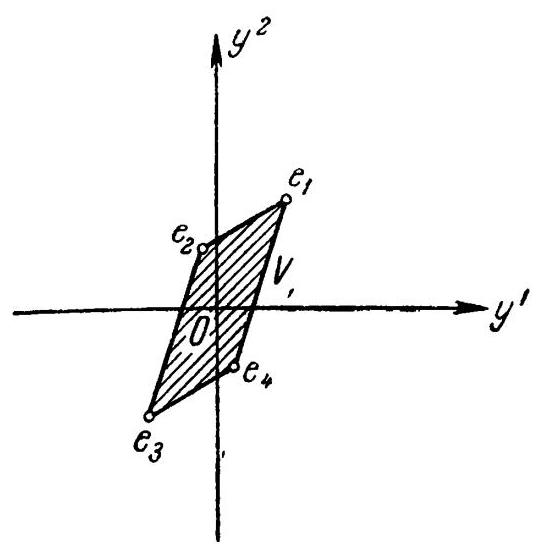
\includegraphics[max width=0.5\textwidth]{images/bo_d547imjef24c73bgfcdg_158_108_1070_543_550_0.jpg}
\end{center}
\hspace*{3em}

Pac. 33.

\(\alpha\)

\({e}_{1}\)

C2 \({\alpha }_{1}\)

公

C4

\({\alpha }_{4}\)

C3

Pnc. 34.

с точностью до общего положительного множителя про- порциональности (ибо функция H однородна относительно величин у,), то мы можем отбросить положительный множитель пропорциональности се вектор и задается соотношениями:

\[
{\psi }_{1} = \cos \left( {{\mu t} + \alpha }\right) ,\;{\psi }_{2} = \sin \left( {{\mu t} + \alpha }\right) .
\]

Иначе говоря, вектор \(\psi  = \left( {{\psi }_{1},{\psi }_{2}}\right)\) равномерно вращается (вокруг начала координат) против часовой стрелки с угло- вой скоростью μ (напомним, что μ > 0).

Обозначим теперь вершины параллелограмма V через \({e}_{1},{e}_{2},{e}_{3},{e}_{4}\), нумеруя их против часовой стрелки. Далее, проведем из начала координат прямые, перпендикуляр- ные сторонам параллелограмма V, и обозначим образуемые этими прямыми углы через \({\alpha }_{1},{\alpha }_{2},{\alpha }_{3},{\alpha }_{4}\) (рис. 3). Так как функция \(H\) в рассматриваемом случае имеет вид

\[
H = \ldots  + {\psi }_{1}{v}^{1} + {\psi }_{2}{v}^{2} = \ldots  + \left( {\psi ,v}\right)
\]

(многоточием обозначены члены, не содержащие у и и’), то из рис. 35 ясно, что если вектор ф находится в угле \({\alpha }_{i}\left( {i = 1,2,3,4}\right)\), то мак- симум функции \(H\) npu \(v \in  V\) достигается в верши- не \(v = {e}_{i}\). Вспомнив теперь, что вектор ф равномер- но вращается с угловой скоростью μ, мы приходим к следующему выводу от- носительно оптимальных управлений. В течение вре- мени д у управляющий га- раметр v имеет значение \({e}_{i}\), затем v «переключается» в вершину \({e}_{i + 1}\),где находит- ся в течение времени \(\frac{{\alpha }_{i + 1}}{\mu }\) (при \(i = 4\) следует считать, что \(i + 1 = 1\) ), после этого «переключается» в вершину \({e}_{i + 2}\) и т. д. При этом пер- вый и последний отрезки времени могут быть меньше соответствующих величин д му, так как в начальный момент движение могло начаться не в момент «переключения», а в конце движение может прекратиться (т. е. фазовая точка попадет в начало координат) до момента очередного переключения.

\begin{center}
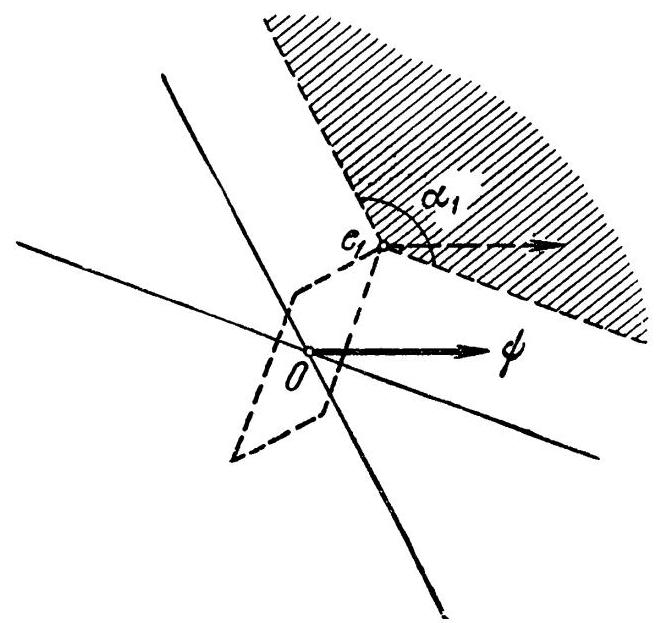
\includegraphics[max width=0.6\textwidth]{images/bo_d547imjef24c73bgfcdg_159_115_734_658_623_0.jpg}
\end{center}
\hspace*{3em}

Pnc. 35.

Обозначим теперь через е, такую точку (а й, а?) плоско- сти я, координаты которой удовлетворяют соотношениям

\[
\left. \begin{array}{l} \lambda {a}_{i}^{1} - \mu {a}_{i}^{2} =  - {v}_{i}^{1}, \\  \mu {a}_{i}^{1} + \lambda {a}_{i}^{2} =  - {v}_{i}^{2}, \end{array}\right\} \tag{51}
\]

где \({v}_{i}^{1},{v}_{i}^{2} -\) координаты вершины \({e}_{i}\) параллелограмма \(V\).

Тогда мы получим четыре точки е, где мы являющиеся вершинами некоторого параллелограмма V′ (ибо соотно- шения (51) линейны). Из вида формул (51) легко выте- кает, что параллелограмм V′ получается из \(V\) подобным преобразованием (с центром в начале) и поворотом на некоторый угол (рис. 36). Из формул (50), (51) выте- кает, что в то время, когда управляющий параметр и принимает значение \({e}_{i}\), \(\mathbf{u}3\) менение координат \({y}^{1}\), \({y}^{2}\) описывается уравнениями

\[
\left. \begin{array}{l} \frac{d{y}^{1}}{dt} = \lambda \left( {{y}^{1} - {a}_{i}^{1}}\right)  - \mu \left( {{y}^{2} - {a}_{i}^{2}}\right) , \\  \frac{d{y}^{2}}{dt} = \mu \left( {{y}^{1} - {a}_{i}^{1}}\right)  + \lambda \left( {{y}^{2} - {a}_{i}^{2}}\right)  \end{array}\right\}
\]

\[
{\left( {52}\right) }_{i}
\]

Сравнивая систему (52) с системой

\[
\left. \begin{array}{l} \frac{d{y}^{1}}{dt} = \lambda {y}^{1} - \mu {y}^{2}, \\  \frac{d{y}^{2}}{dt} = \mu {y}^{1} + \lambda {y}^{2}, \end{array}\right\} \tag{53}
\]

мы видим, что «фазовые портреты» систем (52) и (53) получаются друг из друга параллельным переносом; именно, положение равнове- сия системы (52), расположе- но не в начале координат (как у системы (53), рис. 37), а в точке е, а

\begin{center}
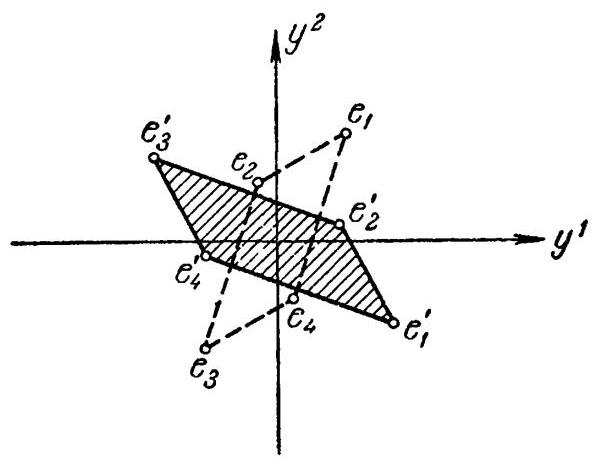
\includegraphics[max width=0.5\textwidth]{images/bo_d547imjef24c73bgfcdg_160_824_1339_595_457_0.jpg}
\end{center}
\hspace*{3em}

Purc. 36.

Вспоминая сказанное вы- ше о характере оптимальных управлений, мы получаем сле- дующее утверждение о струк- туре оптимальных траекто- рий. В течение времени \(\frac{{\alpha }_{i}}{\mu }\) точ- ка описывает дугу фазовой траектории системы (52), затем в течение времени д меня тере движение описывается системой \({\left( {52}\right) }_{i + 1}\), после этого вступает в действие система (52) \({}_{i + 2}\) и т. д. (первый и последний отрезки времени могут быть меньше, чем соответствующие величины \(\frac{{\alpha }_{i}}{\mu }\) ).

6 Л. С. Понтрягин и др.

Tenepb уже нетрудно построить на плоскости π «линии переключения», определяющие синтез оптималь- ных управлений. Обозначим через A 10 (i = 1, 2, 3, 4) дугу траектории системы (52), оканчивающуюся в точке O и соответствующую отрезку времени да (нис. 38). Тогда ясно, что за к лю чит е л ь н ы й этап оптимального движения фазовой точки происходит по одной из дуг \({A}_{i}O\), причем точка может пройти не всю эту дугу, а лишь некоторую ее часть \({X}_{i}O\) (так как последний отрезок вре- мени может быть меньше, чем д д далее, так как в точке \({X}_{i}\) произошло «переключение», и фазовая точка после «переключения» стала двигаться согласно системе (52), то п е р е д моментом переключения фазовая точка двига- лась по закону (51)i—1. Таким образом, предыдущий отре- 30K \({Y}_{i}{X}_{i}\) оптимальной траектории представляет собой дугу траектории системы (52) -1, оканчивающуюся в точке \({X}_{i}\) и соответствующую отрезку времени ди \({X}_{i}\) пробегает всю дугу \({A}_{i}O\),дуги \({Y}_{i}{X}_{i}\) указан- ного вида заполняют «криволинейный четы- рехугольник» (рис. 39), одна из «сторон» ко- торого совпадает с ду- roü \({A}_{i - 1}O\) (ató un \({X}_{i} = {O}_{\text{ дуга }}{Y}_{i}{X}_{i}\cos  -\) падает с \({A}_{i - 1}O\) ). Ta- ким образом, три вершины рассматриваемого криволинейного четырех- угольника находятся в точках \({A}_{i},O,{A}_{i - 1}\) ; четвертую вершину обозначим через \({B}_{i - 1}\). Тогда дуга \({B}_{i - 1}{A}_{i - 1}\) пред-

\begin{center}
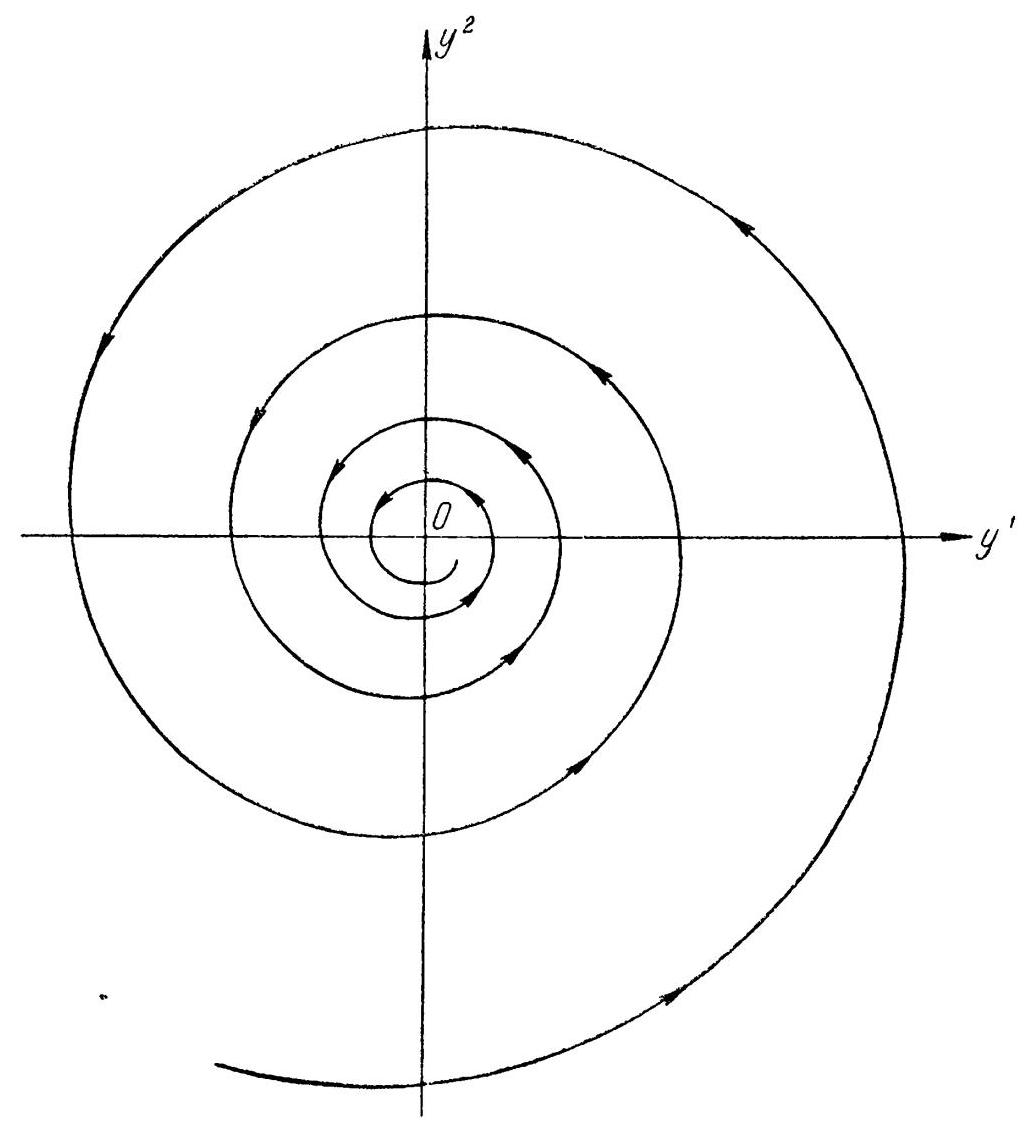
\includegraphics[max width=0.9\textwidth]{images/bo_d547imjef24c73bgfcdg_161_246_417_1033_1128_0.jpg}
\end{center}
\hspace*{3em}

Pac. 37.

\begin{center}
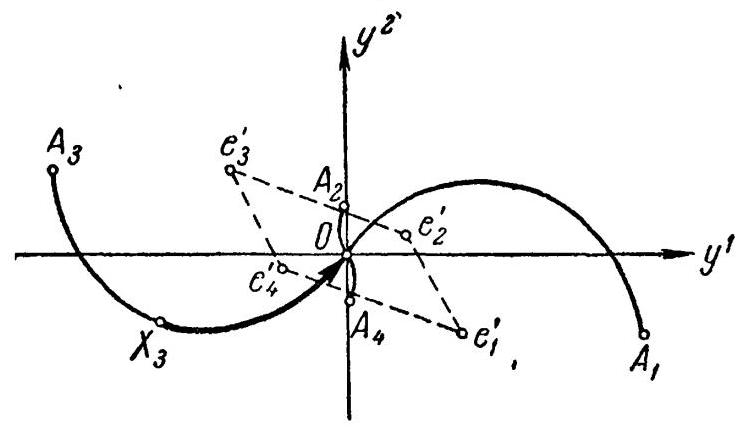
\includegraphics[max width=0.6\textwidth]{images/bo_d547imjef24c73bgfcdg_162_665_503_744_427_0.jpg}
\end{center}
\hspace*{3em}

Pac. 38.

Легко понять, что дуга \({B}_{i - 1}{A}_{i1}\) получа- ется из дуги \({A}_{i}O\) при помощи подобного преобразования с цен- ставляет собой геоме- трическое место точек \(\widetilde{{Y}_{i}}\),т. e. тех точек оп- тимальных траекто- рий, в которых про- исходит переключе- ние (от системы (52) — к системе (52) —).

\begin{center}
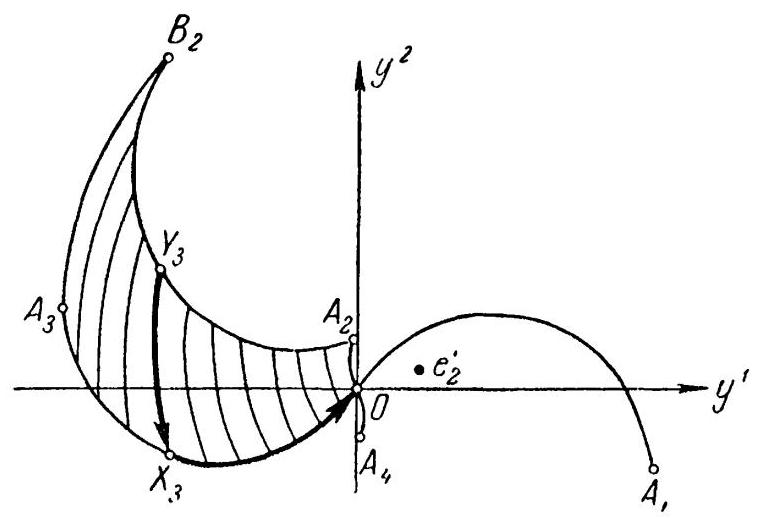
\includegraphics[max width=0.7\textwidth]{images/bo_d547imjef24c73bgfcdg_162_122_1187_761_518_0.jpg}
\end{center}
\hspace*{3em}

Pnc. 39.

тром \({e}_{i - 1}^{\prime }\) и коэффициентом \({e}^{-\frac{\lambda {a}_{i - 1}}{\mu }}\) и и поворота вокруг центра \({e}_{i - 1}^{\prime }\) на угол \({\alpha }_{i - 1}\) по часовой стрелке. В самом де- ле, решения системы (53) в полярных координатах \(\left( {{y}^{1} = \rho \cos \varphi,{y}^{2} = \rho \sin \varphi }\right)\) имеют вид

\[
\rho  = c{e}^{\lambda t},\;\varphi  = {\mu t} + \alpha ,
\]

где \(c > 0\) и α — постоянные интегрирования. Если точка движется по этому закону, то по истечении отрезка вре- мени, имеющего длину т, радиус-вектор движущейся точки увеличивается в ей граз и поворачивается на угол µт. \(\Pi\) ри \(\tau  = \frac{{\alpha }_{i - 1}}{\mu }\) мы и получаем требуемое утверждение: век- тор, идущий из точки высил в точку \({X}_{i}\), получается из вектора, идущего в точку У, (рис. 40), увеличением дли- ны в \({e}^{\frac{\lambda {\alpha }_{i - 1}}{\mu }}\) pas и поворотом на угол \({\alpha }_{i - 1}\) (против часовой стрелки).

\begin{center}
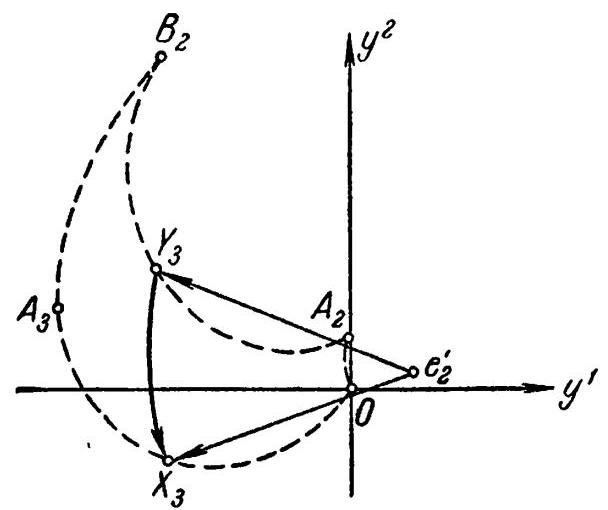
\includegraphics[max width=0.5\textwidth]{images/bo_d547imjef24c73bgfcdg_163_112_324_608_510_0.jpg}
\end{center}
\hspace*{3em}

Prr. 40.

Итак, подобное преобразование с центром ег\_1 и коэф- фициентом \({e}^{-\frac{\lambda {a}_{i - 1}}{\mu }}\), сопровождаемое поворотом (по ча- совой стрелке) на угол \({\alpha }_{i - 1}\),переводит дугу ОА \({}_{i}\) в дугу

\begin{center}
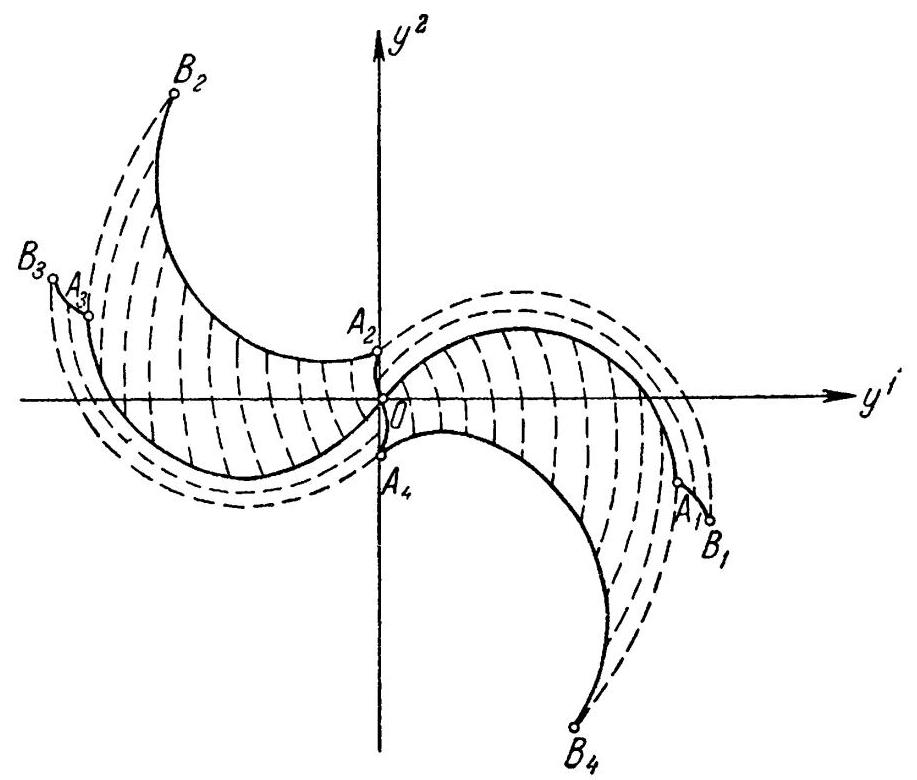
\includegraphics[max width=0.8\textwidth]{images/bo_d547imjef24c73bgfcdg_163_307_1147_917_780_0.jpg}
\end{center}
\hspace*{3em}

Pac. 41.

\({A}_{i - 1}{B}_{i - 1}\) ,на которой происходят «переключения» от систе- мы \({\left( {52}\right) }_{i - 2}\) к системе (52) \({}_{i - 1}\) (puc. 41).

Перед тем как произошло переключение в точке \({Y}_{i}\), фазовая точка двигалась по закону (52).. в течение времени \(\frac{{\alpha }_{i - 2}}{\mu }\) (дуга \({Z}_{i}{Y}_{i}\) на рис. 42). Когда точка \({Y}_{i}\) пробегает всю дугу \({A}_{i - 1}{B}_{i - 1}\),дуги \({Z}_{i}{Y}_{i}\) указанного вида заполняют «криволинейный четырехугольник», двумя сто- ронами которого являются дуги \({A}_{i - 1}{B}_{i - 1}\) и \({A}_{i - 1}{B}_{i - 2}\).

\begin{center}
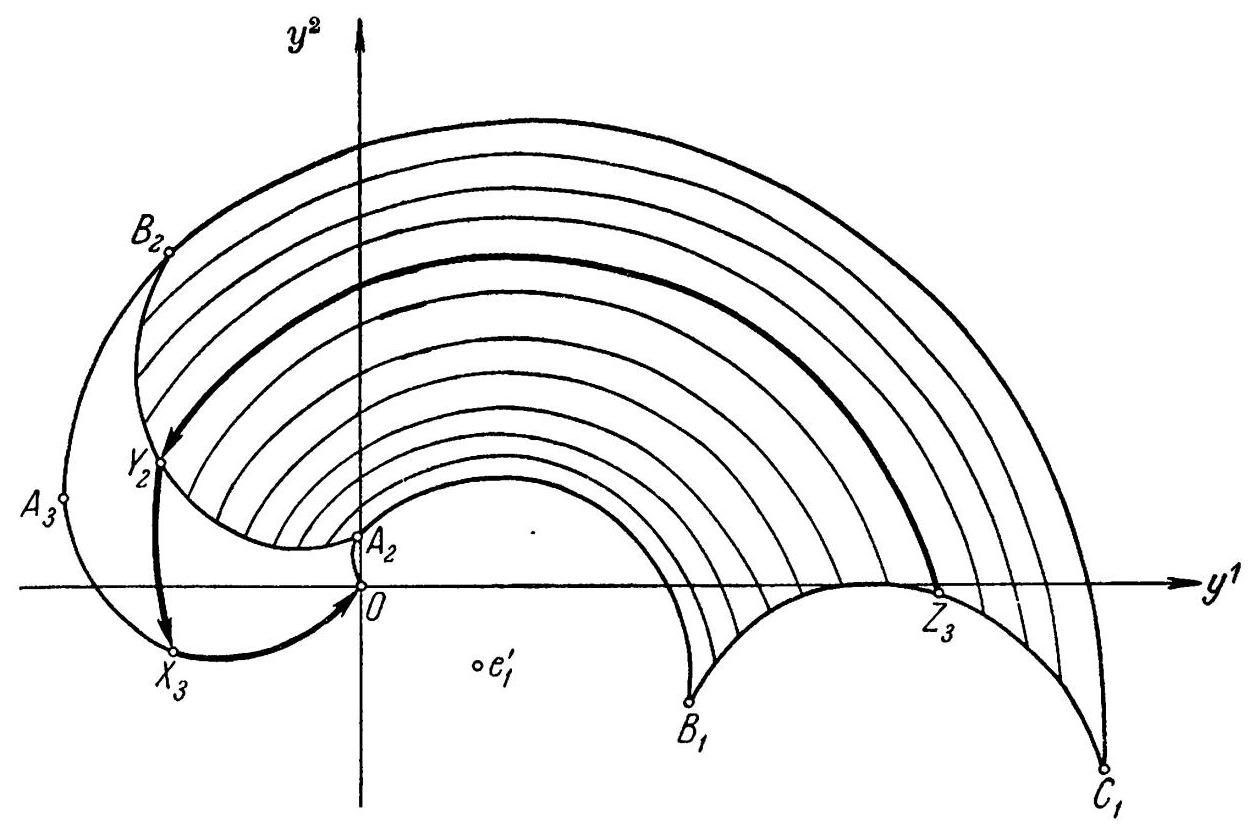
\includegraphics[max width=1.0\textwidth]{images/bo_d547imjef24c73bgfcdg_164_132_474_1258_829_0.jpg}
\end{center}
\hspace*{3em}

Pnc. 42.

Четвертую вершину этого четырехугольника мы обозна- чим через \({C}_{i - 2}\). Как и выше, устанавливается, что дуга \({B}_{i - 2}{C}_{i - 2}\) (геометрическое место предыдущих точек переклю- чения) получается из дуги \({A}_{i - 1}{B}_{i - 1}\) npu помощи подобного преобразования с центром \({e}_{i - 2}^{\prime }\) и коэффициентом \({e}^{-\frac{\lambda {\alpha }_{i - 2}}{\mu }}\), сопровождаемого поворотом (по часовой стрелке) на угол \({\alpha }_{i - 2}\) вокруг центра е \({e}_{i - 2}^{\prime }\).

Продолжая таким образом, мы вычертим четыре линии \(O{A}_{i}{B}_{i}{C}_{i}{D}_{i}\ldots \left( {i = 1,2,3,4}\right)\),исходящие из начала коор- динат и представляющие в совокупности геометрическое место точек переключения (рис. 43). Подобное преобразо- вание с центром \({e}_{i - 1}^{\prime }\) и коэффициентом \({e}^{-\frac{\lambda {a}_{i - 1}}{\mu }}\), compo- вождаемое поворотом вокруг точки е на та тя и угол а та-та совой стрелке, переводит линию ОА \({}_{i}{B}_{i}{C}_{i}\cdots\) в линию \({A}_{i - 1}{B}_{i - 1}{C}_{i - 1}{D}_{i - 1}\ldots\) (puc. 44). Это позволяет последовательно вычерчивать части линий \(O{A}_{i}{B}_{i}{C}_{i}\ldots,\) зная первые куски \({\mathrm{{OA}}}_{1},{\mathrm{{OA}}}_{2},{\mathrm{{OA}}}_{3},{\mathrm{{OA}}}_{4}\) этих линий (определение этих кусков

\begin{center}
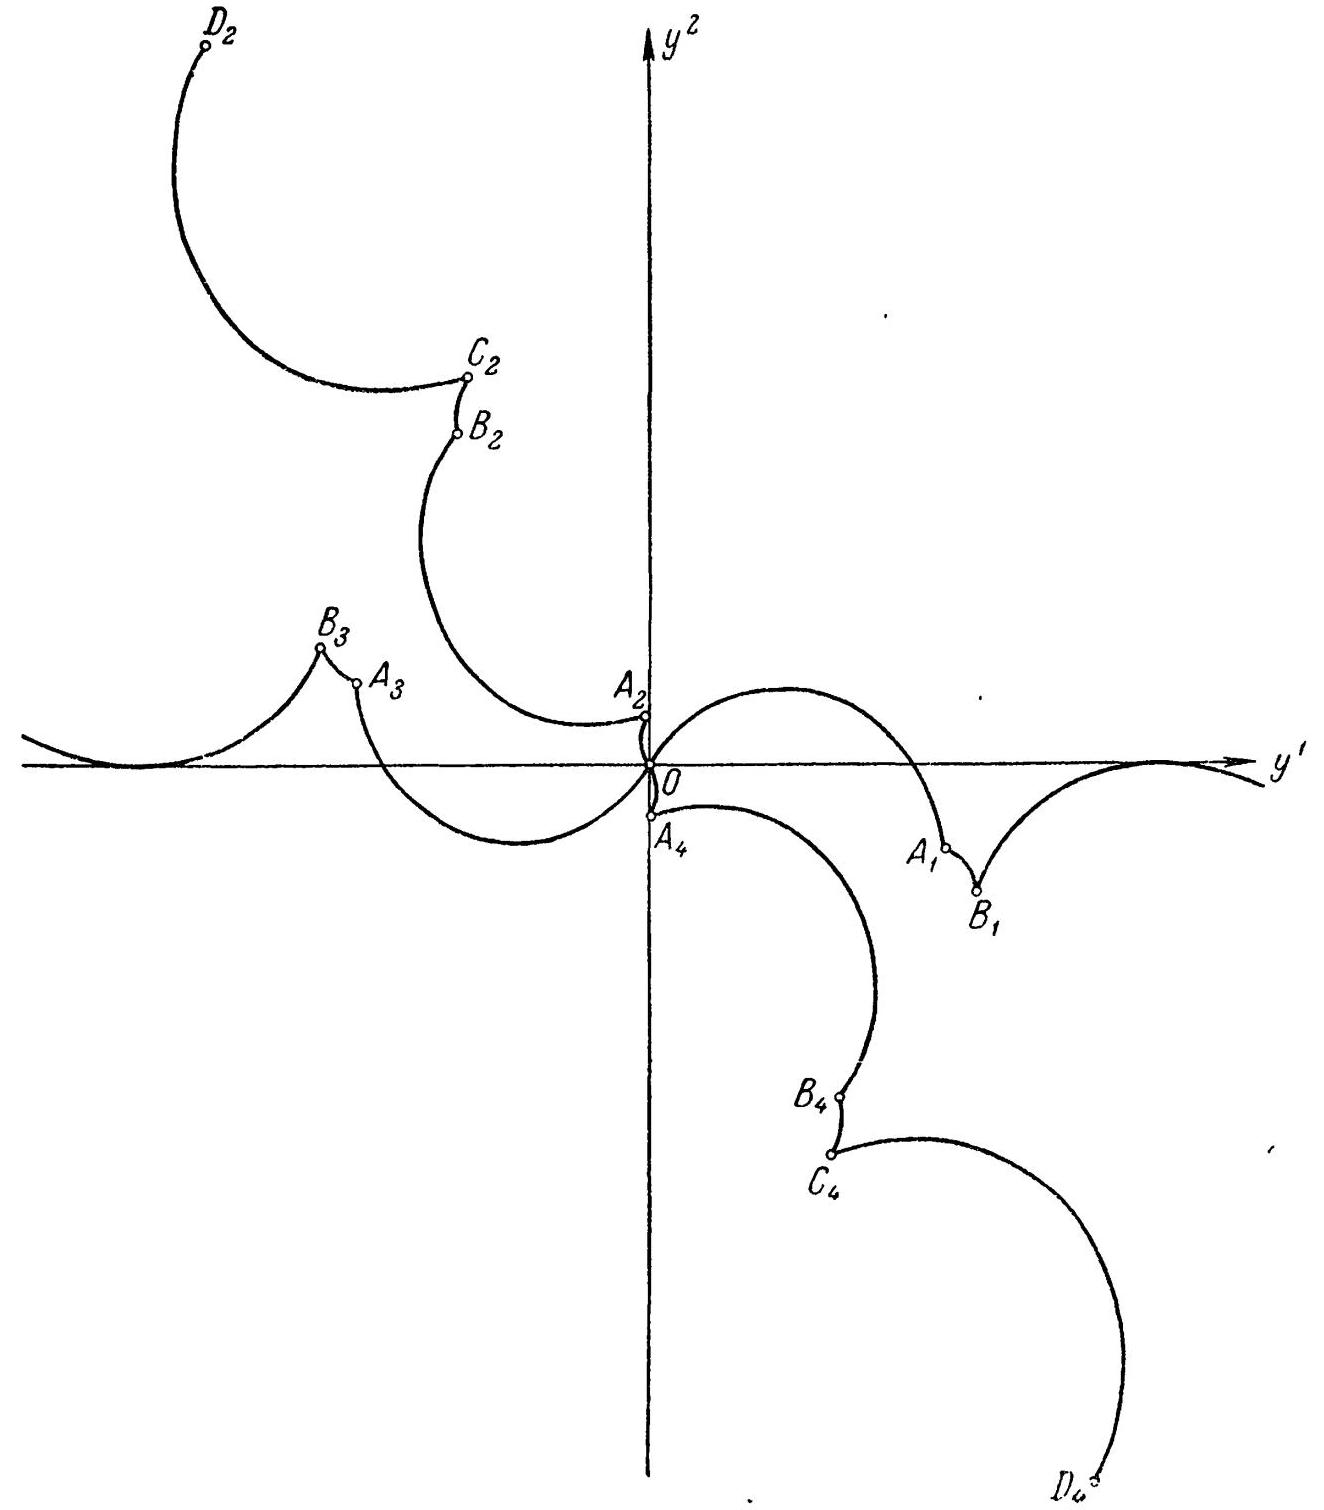
\includegraphics[max width=1.0\textwidth]{images/bo_d547imjef24c73bgfcdg_165_99_434_1324_1510_0.jpg}
\end{center}
\hspace*{3em}

Рис. 43.

было приведено выше). Остается заметить, что значение \({e}_{i}\) управляющий параметр v принимает внутри «угла» между линиями \({\mathrm{{OA}}}_{i + 1}{B}_{i + 1}{C}_{i + 1}\ldots\) и \({\mathrm{{OA}}}_{i}{B}_{i}{C}_{i}\ldots\) и на дуге \({A}_{i}O\). Это и дает синтез оптимальных управлений (рис. 45). Вид оптимальных траекторий показан на рис. 46.

Напомним, что рисунки 37-46, рассмотренные выше, относились к случаю, когда λ<0, т. е. когда собственные осуществляется во всей плоскости π. При \(\lambda  = 0\) размеры дуг не меняются (т. е. \(O{A}_{i} = {B}_{i}{C}_{i} = \ldots\), \(\left. {{A}_{i}{B}_{i} = {C}_{i}{D}_{i},\ldots }\right)\) ; синтез оптимальных управлений по-преж- нему осуществляется во всей плоскости π (см. пример 3

\begin{center}
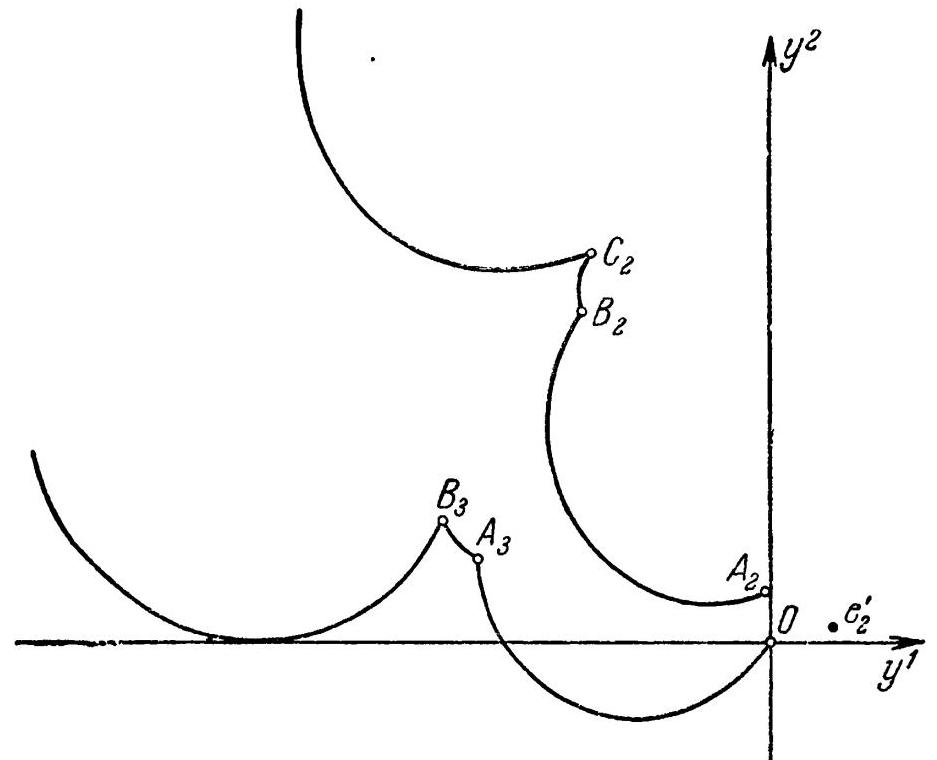
\includegraphics[max width=0.8\textwidth]{images/bo_d547imjef24c73bgfcdg_166_290_318_937_760_0.jpg}
\end{center}
\hspace*{3em}

Pur. 44.

\begin{center}
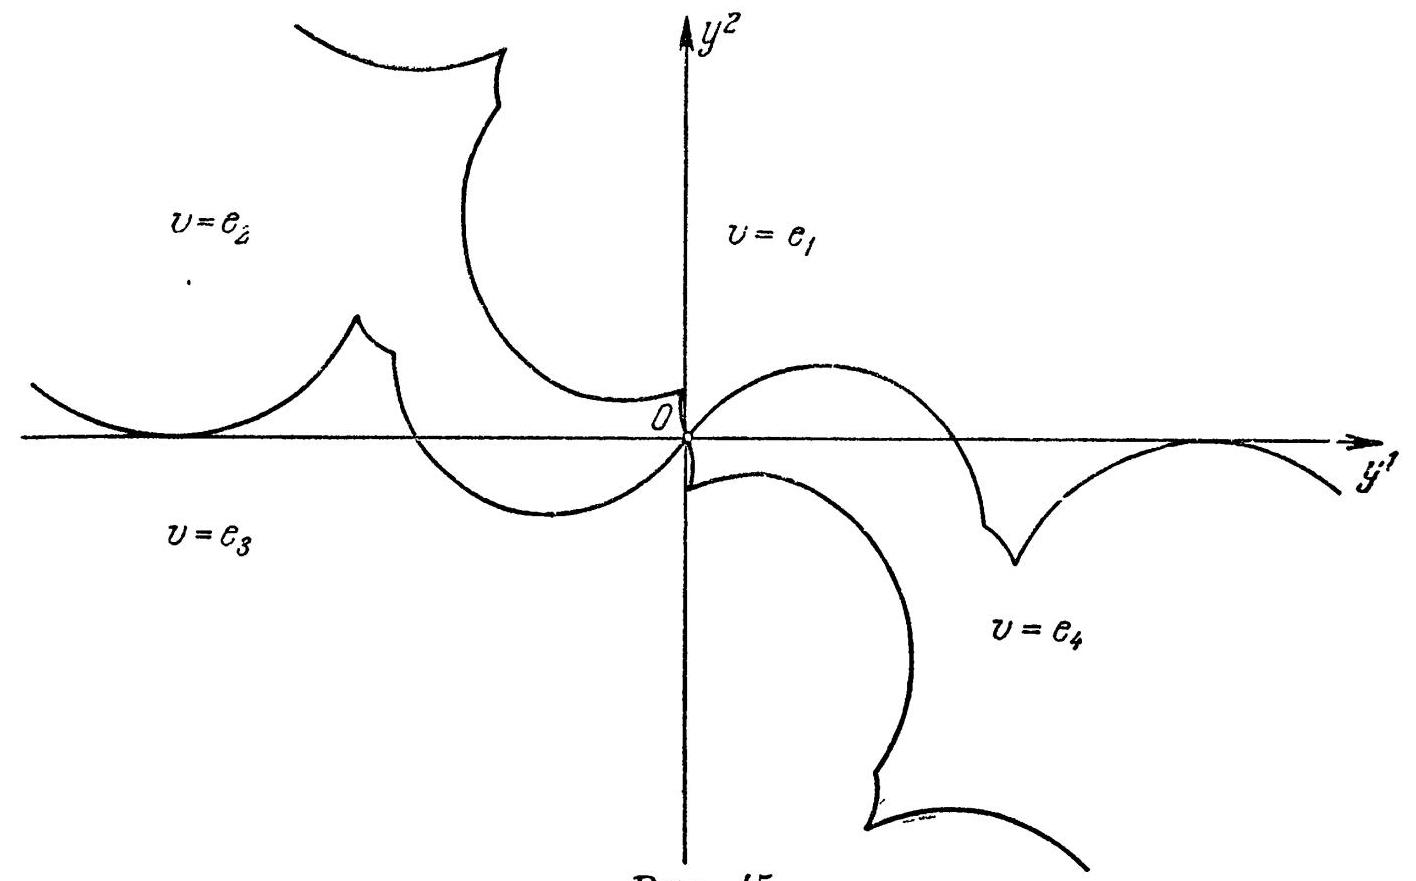
\includegraphics[max width=1.0\textwidth]{images/bo_d547imjef24c73bgfcdg_166_46_1130_1416_881_0.jpg}
\end{center}
\hspace*{3em}

Puc. 45.

значения матрицы (а/і) имеют отрицательные действитель- ные части. В этом случае размеры дуг \(O{A}_{i},{A}_{i}{B}_{i},{B}_{i}{C}_{i},\ldots\) увеличивались, а синтез оптимальных управлений

\begin{center}
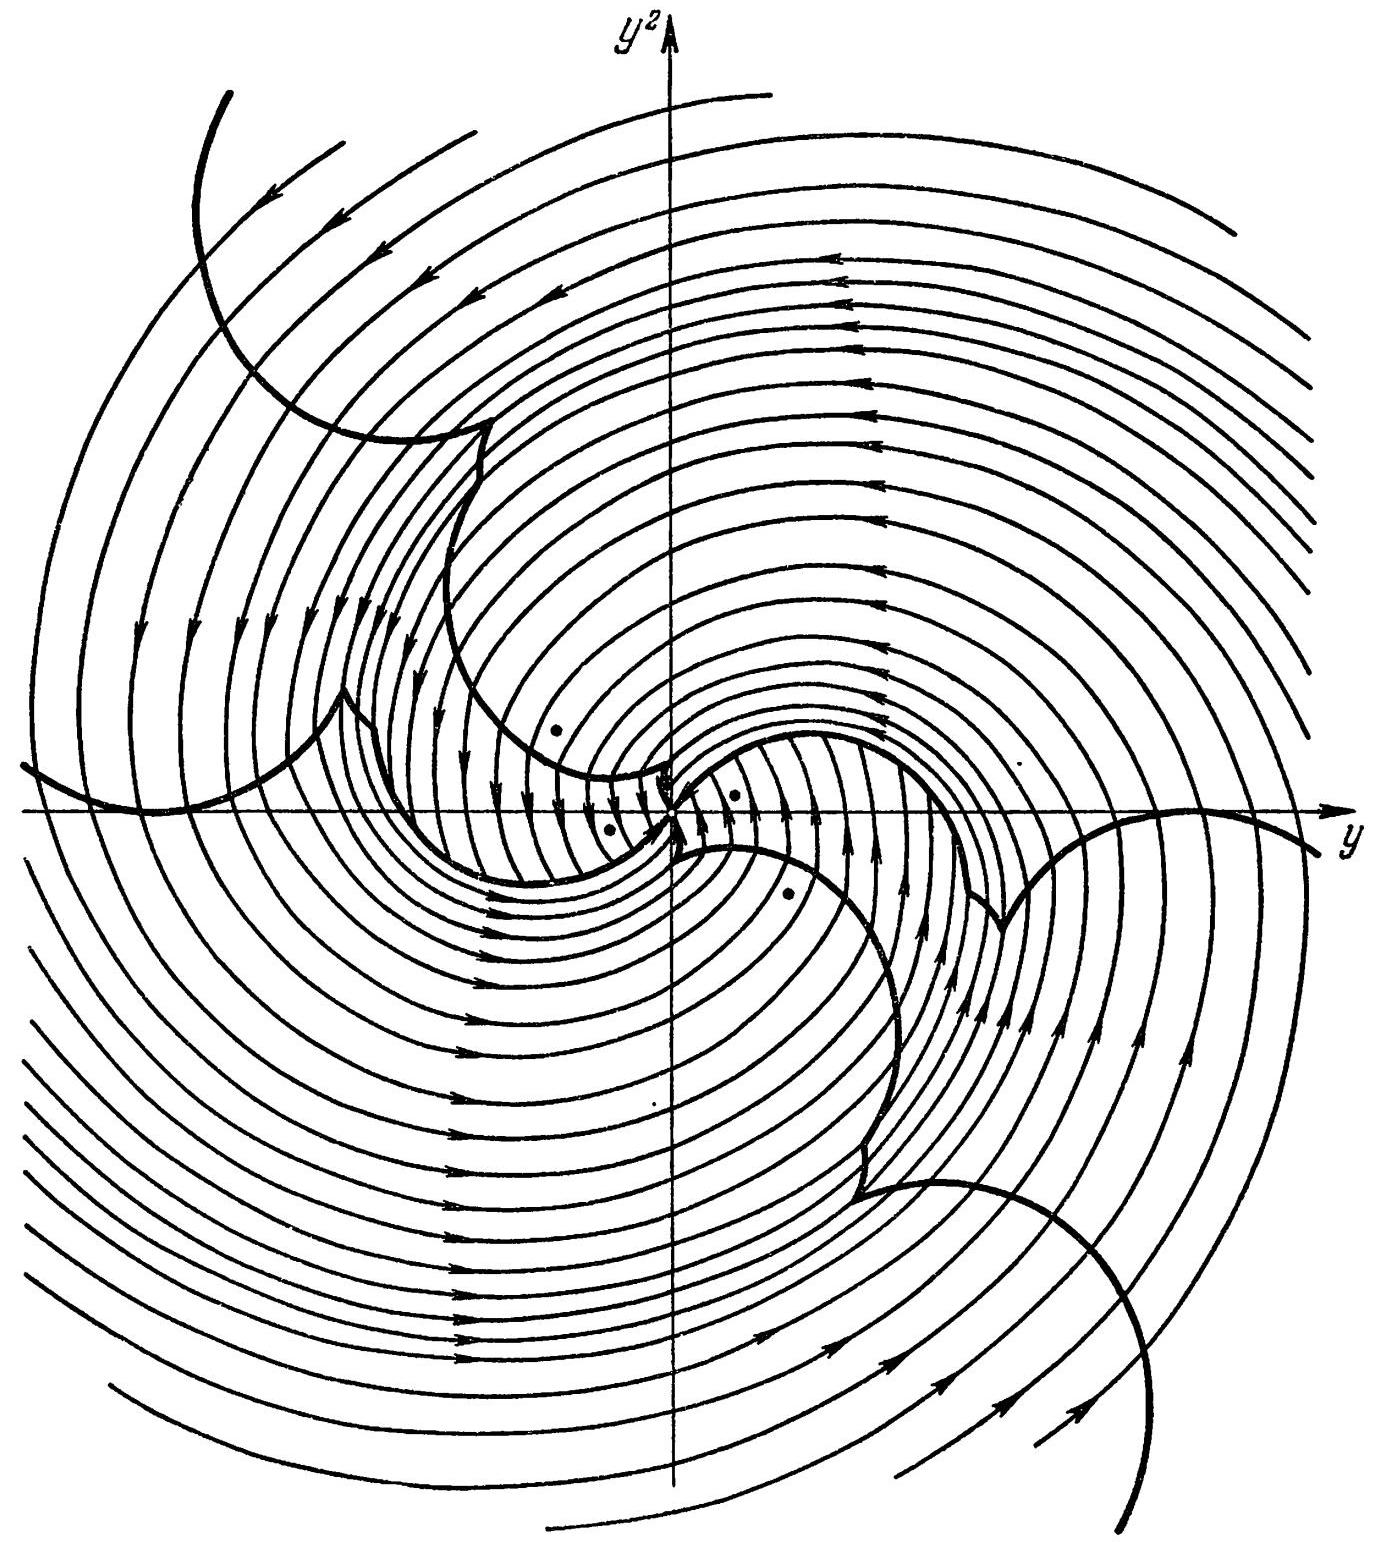
\includegraphics[max width=1.0\textwidth]{images/bo_d547imjef24c73bgfcdg_167_72_410_1374_1542_0.jpg}
\end{center}
\hspace*{3em}

Pnc. 46.

в § 5). Наконец при \(\lambda  > 0\) размеры дуг \(O{A}_{i},{B}_{i}{C}_{i},\ldots\), а также дуг \({A}_{i}{B}_{i},{C}_{i}{D}_{i},\ldots\) уменьшаются в геометрической прогрессии; синтез оптимальных управлений осущест- вляется лишь в ограниченном куске плоскости π (рис. 47).

Bce сказанное относится к синтезу оптимальных управлений в плоскости π переменных \({y}^{1},{y}^{2}\). Переход

\begin{center}
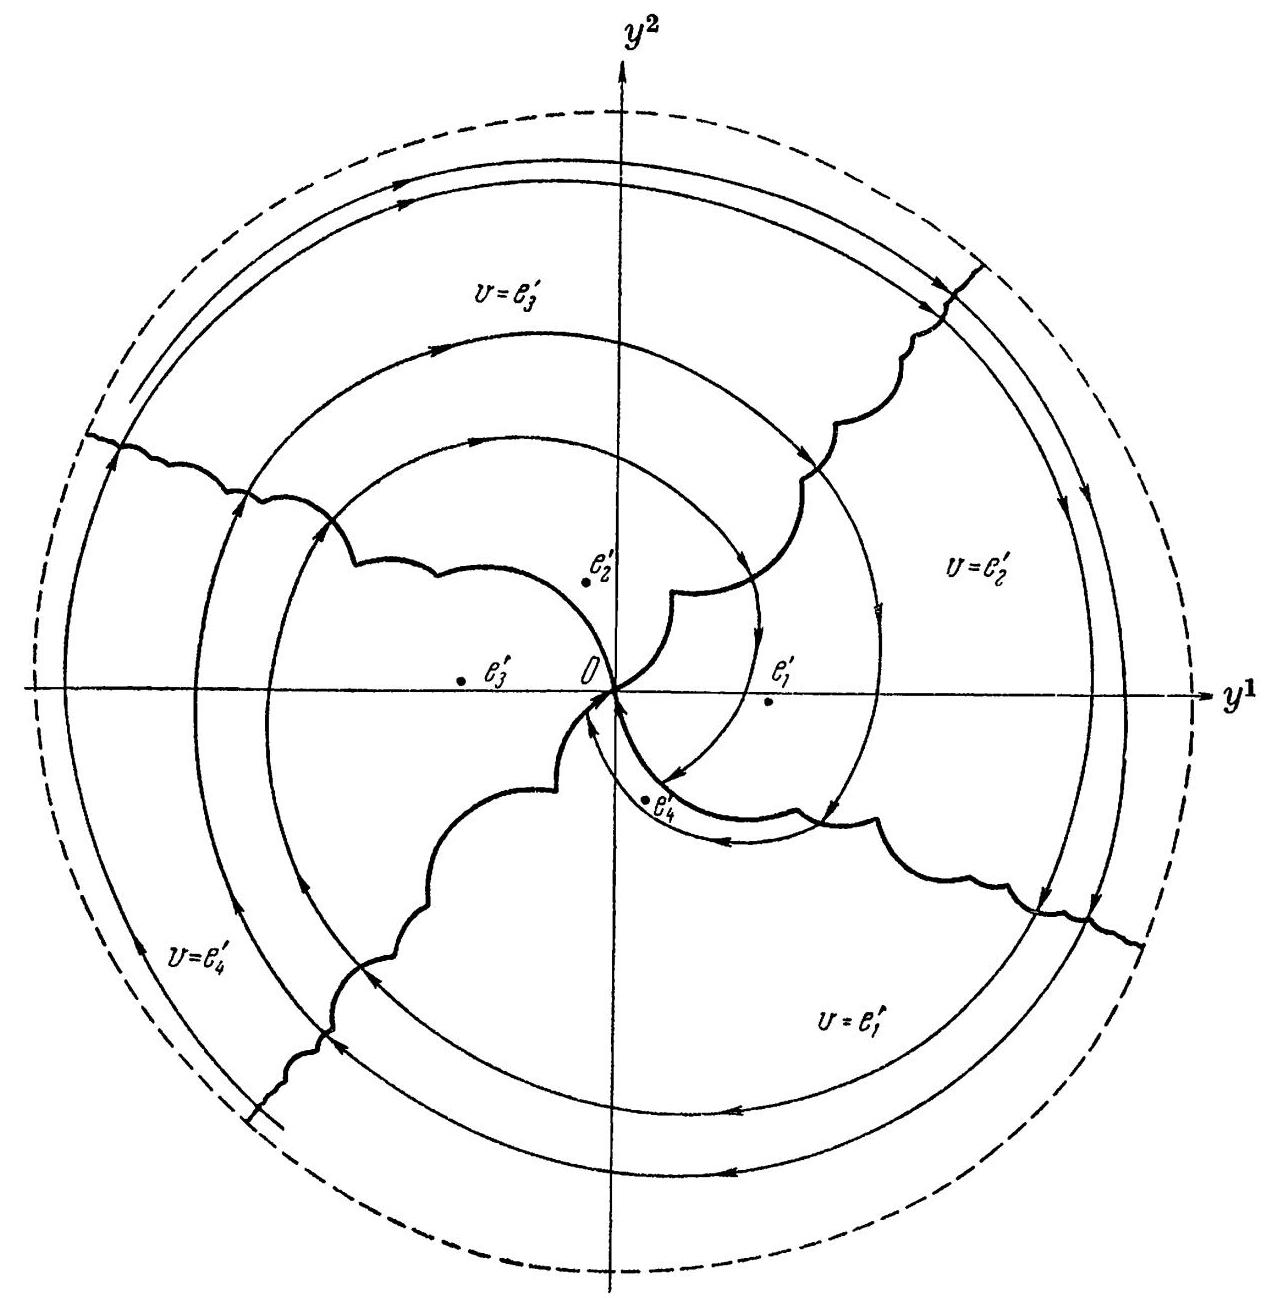
\includegraphics[max width=1.0\textwidth]{images/bo_d547imjef24c73bgfcdg_168_148_315_1270_1298_0.jpg}
\end{center}
\hspace*{3em}

Pnc. 47.

к плоскости \(X\) исходных переменных \({x}^{1},{x}^{2}\) осуществ- ляется по формулам (47). Картина синтеза оптимальных управлений при этом аффинно искажается.

\(\Pi\) p \(u\) м е р 2

(Система второго порядка с двумя управляющими параметрами и отрицательными собственными значениями.)

Рассмотрим систему (45) в предположении, что соб- ственные значения матрицы ( \({a}_{j}^{i}\) ) действительны, отри- цательны и различны. Мы по-прежнему будем пред- полагать, что область управления U определяется неравенствами (46) и что определитель матрицы \(\left( {b}_{j}^{i}\right)\) отли- чен от нуля. Обозначим собственные значения матрицы \(\left( {a}_{j}^{i}\right)\) через \({\lambda }_{1}\) и \({\lambda }_{2}\),причем ль слу с 0. Линейным пре- образованием переменных (см. (47)) систему (45) можно привести к виду

\[
\left. \begin{array}{l} \frac{d{y}^{1}}{dt} = {\lambda }_{1}{y}^{1} + {c}_{1}^{1}{u}^{1} + {c}_{2}^{1}{u}^{2}, \\  \frac{d{y}^{2}}{dt} = {\lambda }_{2}{y}^{2} + {c}_{1}^{2}{u}^{1} + {c}_{2}^{2}{u}^{2}, \end{array}\right\}
\]

или, иначе, к виду

\[
\left. \begin{array}{l} \frac{d{y}^{1}}{dt} = {\lambda }_{1}{y}^{1} + {v}^{1}, \\  \frac{d{y}^{2}}{dt} = {\lambda }_{2}{y}^{2} + {v}^{2}, \end{array}\right\} \tag{54}
\]

(см. (49)). Как и в первом примере, точка у = ( \({v}^{1}\), \({v}^{2}\) ) описывает в плоскости π переменных у 1, у 2 параллело- гратм \(V\) (puc. 33).

Система (5) принимает в случае управляемого про- цесса (54) следующий вид:

\[
\left. \begin{array}{l} \frac{d{\psi }_{1}}{dt} =  - {\lambda }_{1}{\psi }_{1}, \\  \frac{d{\psi }_{2}}{dt} =  - {\lambda }_{2}{\psi }_{2}; \end{array}\right\}
\]

ee oórroe perreture:

\[
{\psi }_{1} = {c}_{1}{e}^{-{\lambda }_{1}t},\;{\psi }_{2} = {c}_{2}{e}^{-{\lambda }_{2}t}.
\]

Из этих формул видно, что если одна из постоянных интегрирования \({c}_{1},{c}_{2}\) равна нулю, то вектор \(\psi  = \left( {{\psi }_{1},{\psi }_{2}}\right)\) сохраняет постоянное направление (параллельное одной из осей координат). Если же оба числа с, с отличны от нуля, то вектор ф монотонно поворачивается (с воз- растанием н) от оси абсписс к оси ординат, оставаясь все время в одном квадранте (πбо \(\left| \frac{{\psi }_{2}}{{\psi }_{1}}\right|  = \left| \frac{{c}_{2}}{{c}_{1}}\right| {e}^{\left( {{\lambda }_{1} - {\lambda }_{2}}\right) t} \rightarrow  \infty\) при возрастании t).

Для системы (45) мы предполагаем выполненным условие общности положения; тогда для системы (54), получающейся из нее линейным преобразованием, это условие также выполнено. Иначе говоря, ни одна из сторон параллелограмма V не параллельна ни одной из осей координат. Проведя из начала координат прямые \({l}_{1},{l}_{2}\), перпендикулярные сторонам параллелограмма V (рис. 34; эти прямые отличны от осей координат в силу сказанного выше), мы, как и прежде, найдем, что если вектор \(\psi\) находится в угле а, (i = 1, 2, 3, 4), то максимум функции \(H\) npu \(v \in  V\) достигается в вершине \(v = {e}_{i}\) (рис. 35).

Обозначим теперь через ег точку (а c координатами

\[
{a}_{i}^{1} =  - \frac{1}{{\lambda }_{1}}{v}_{i}^{1},\;{a}_{i}^{2} =  - \frac{1}{{\lambda }_{2}}{v}_{i}^{2}, \tag{55}
\]

где \({v}_{i}^{1},{v}_{i}^{2}\) - координаты вершины \({e}_{i}\) параллелограмма V. Тогда мы получим четыре точки е, i, e дол ей, являющиеся вершинами некоторого параллелограмма V'. Из формул (54), (55) вытекает, что в то время, когда управляющий параметр v принимает значение \({e}_{i}\), изменение координат \({y}^{1},{y}^{2}\) описнвается уравнениями

\[
\left. \begin{array}{l} \frac{d{y}^{1}}{dt} = {\lambda }_{1}\left( {{y}^{1} - {a}_{i}^{1}}\right) , \\  \frac{d{y}^{2}}{dt} = {\lambda }_{2}\left( {{y}^{2} - {a}_{i}^{2}}\right)  \end{array}\right\}
\]

\[
{\left( {56}\right) }_{i}
\]

«Фазовый портрет» системы (56), получается из «фазово- го портрета» системы

\[
\left. \begin{array}{l} \frac{d{y}^{1}}{dt} = {\lambda }_{1}{y}^{1}, \\  \frac{d{y}^{2}}{dt} = {\lambda }_{2}{y}^{2} \end{array}\right\} \tag{57}
\]

с помощью параллельного переноса; именно, положение равновесия системы (56), расположено не в начале коор- динат (как у системы (57), рис. 48), а в точке е, к

Дальнейшее исследование приведет к сушественно различным результатам в зависимости от того, как рас- положены прямые \({l}_{1}\) и \({l}_{2}\),перпендикулярные к сторонам параллелограмма V. Мы выделим следующие два случая.

Случай I. Прямые и и и и срасположены в различных квадрантах (т. е. одна в первом и третьем, а другая — во втором и четвертом квадрантах, рис. 49). Произведем нумерацию углов \({\alpha }_{i}\) (определяемых прямыми \({l}_{1}\) и \({l}_{2}\) ) так, как указано на рис. 50. Эта нумерация соответствует тому, что через \({e}_{2}\) и \({e}_{4}\) обозначены соответственно верх- няя и нижняя вершины параллелограмма V, а через \({e}_{1}\) и \({e}_{3} -\) правая и левая (рис. 49). Вспо- миная сказанное выше о характере изменения величин ц и и, мы приходим к следующе- му выводу относитель- но оптимальных управ- лений. Каждое опти- мальное управление либо совсем не содер- жит переключений (т.е. в течение всего движения параметр v сохраняет постоян- ное значение, совпадающее с одной из вершин параллело-

\begin{center}
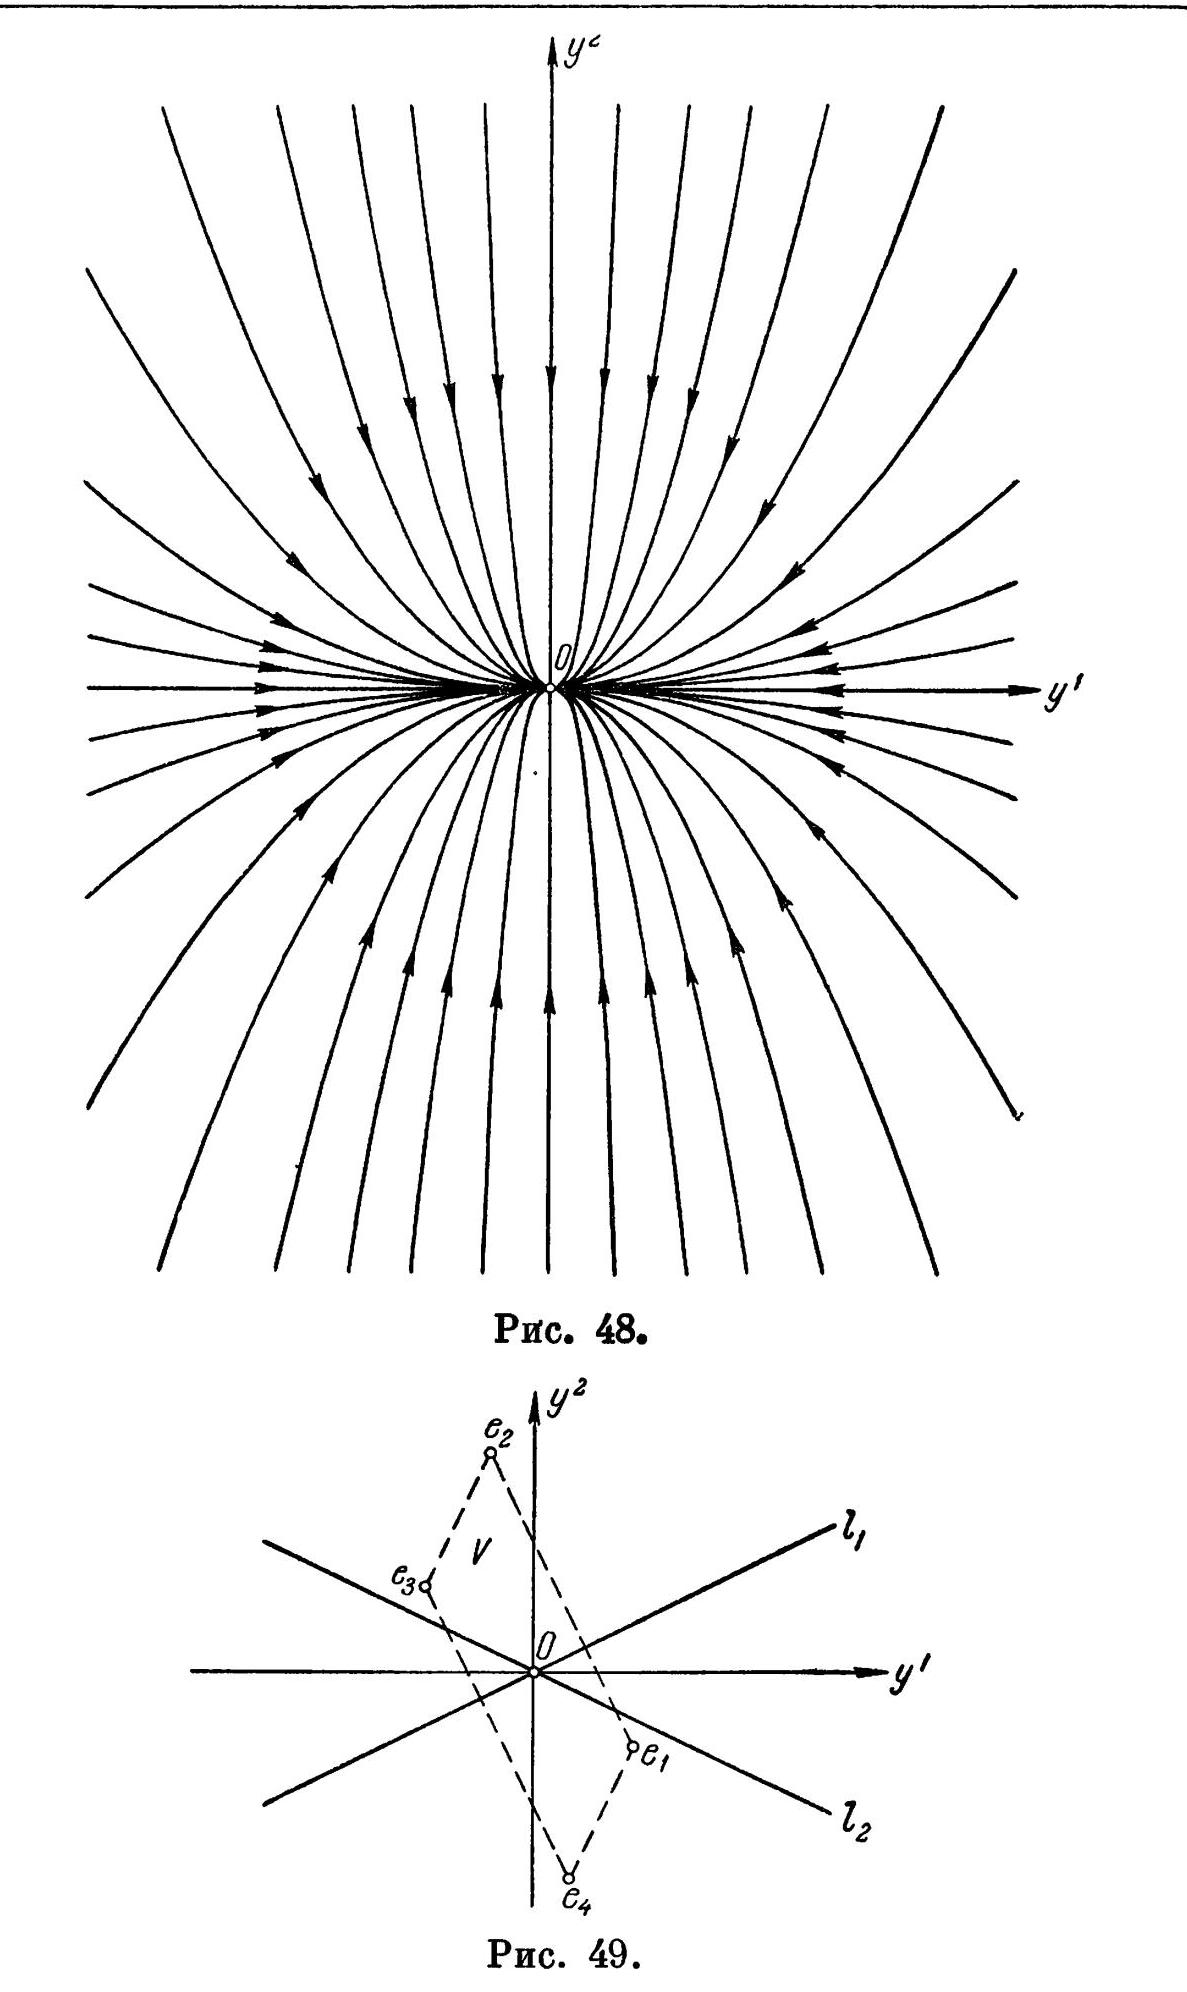
\includegraphics[max width=1.0\textwidth]{images/bo_d547imjef24c73bgfcdg_171_196_207_1187_1992_0.jpg}
\end{center}
\hspace*{3em}

\begin{center}
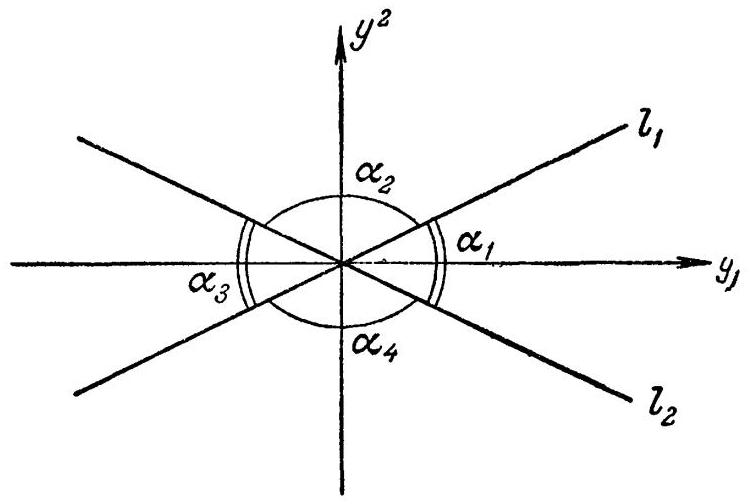
\includegraphics[max width=0.6\textwidth]{images/bo_d547imjef24c73bgfcdg_172_653_347_750_504_0.jpg}
\end{center}
\hspace*{3em}

Pac. 50.

Теперь нетрудно построить на плоскости π «линии пере- ключения», определяющие син- тез оптимальных управлений. Обозначим через АО траекторию системы (56)2, оканчивающуюся в начале координат (рис. 51), а через \({BO} -\) аналогичную траек- торию системы (56)4. Линии АО и ВО симметричны относительно точки O. Если оптимальное движение содержит переклю- чение (только одно в силу грамма V), либо содержит толь- ко одно переключение, и тогда до переключения параметр v сов- падает с одной из вершин е1, \({e}_{3}\), a после переключения — с од- ной из вершин \({e}_{2},{e}_{4}\). сказанного выше), то заключительный этап движе- ния, завершающийся попаданием в начало коорди- нат, происходит в силу системы (56), или (56), т. е. вдоль линии АО или ВО. До этого (т. е. до попадания на линию \({BOA}\) ) точка движется в силу системы (56), или (56), Таким образом, ВОА есть линия переключений, а две области, на которые плоскость разбивается этой линией, заполнены траекториями систем (56), и (56), — правая область, заполнена траекториями системы (56), а левая — траекториями системы (бб)1. Это и дает синтез оптимальных управлений (рис. 52).

\begin{center}
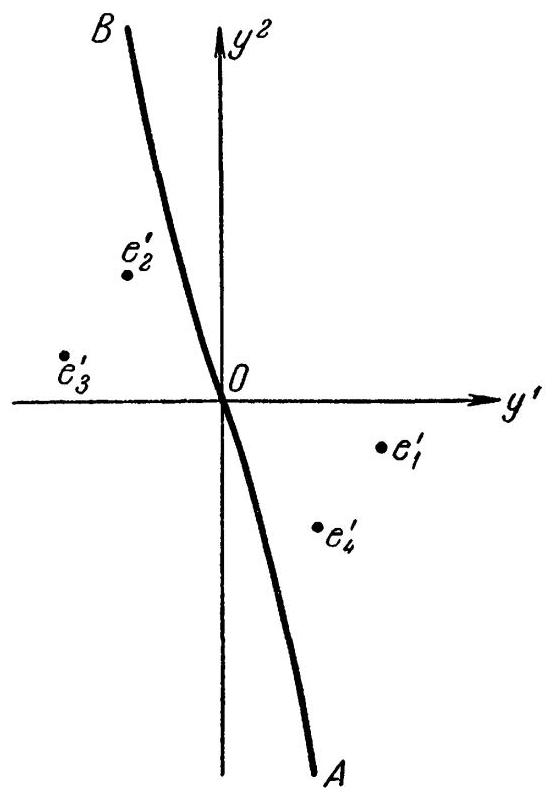
\includegraphics[max width=0.5\textwidth]{images/bo_d547imjef24c73bgfcdg_172_118_1116_552_797_0.jpg}
\end{center}
\hspace*{3em}

Pnc. 51.

\begin{center}
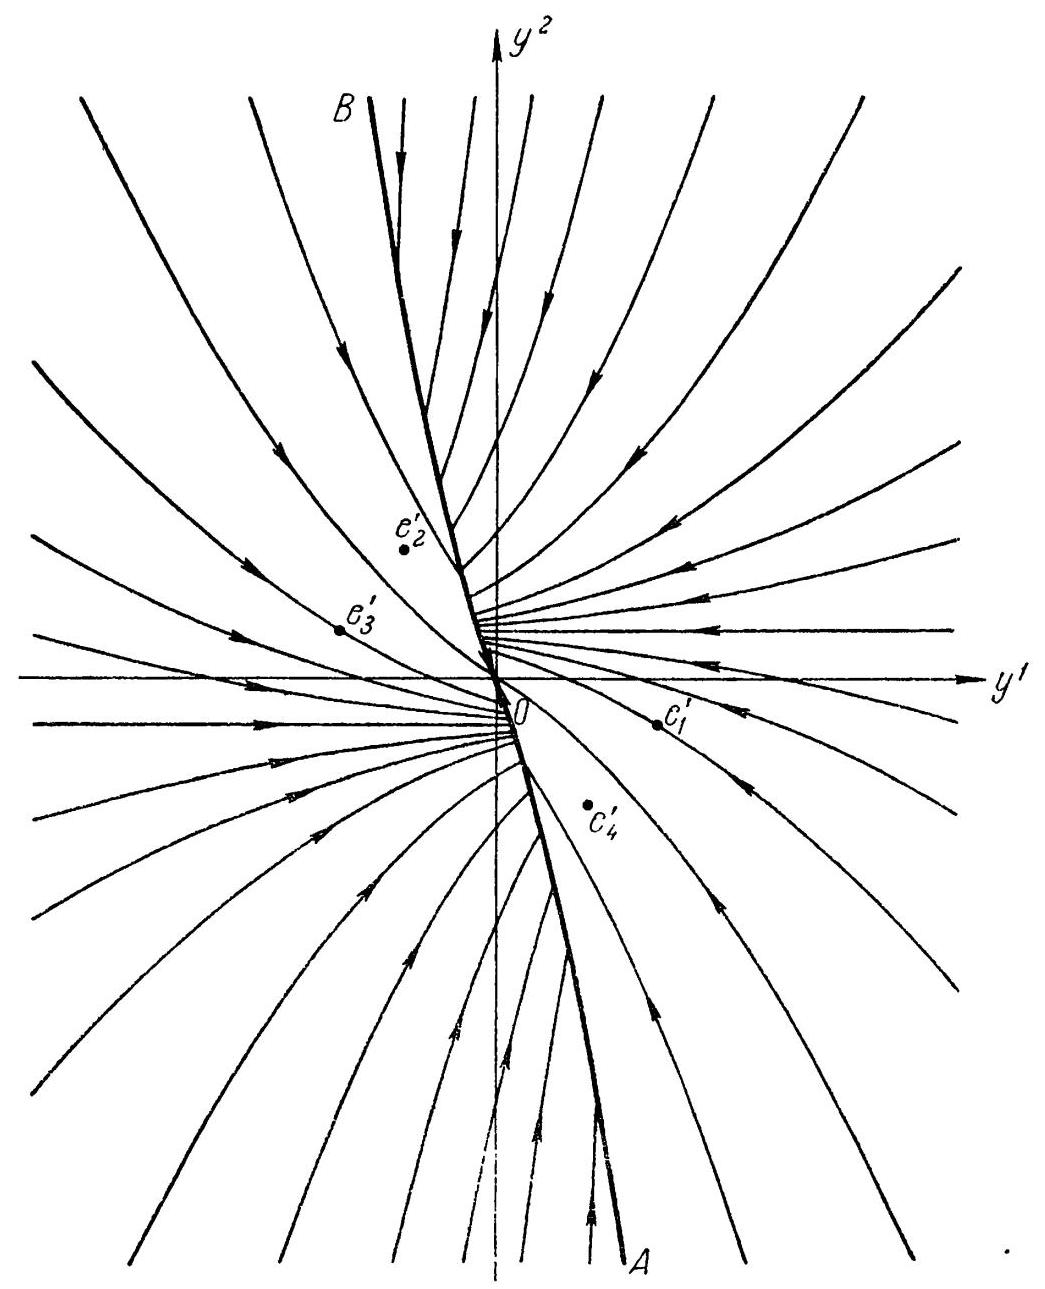
\includegraphics[max width=0.9\textwidth]{images/bo_d547imjef24c73bgfcdg_173_255_388_1045_1289_0.jpg}
\end{center}
\hspace*{3em}

Pac. 52.

При переходе от переменных \({y}^{1},{y}^{2}\) к исходным пере- менным х', хз фазовая картина оптимальных траекторий аффинно искажается.

Случай II. Прямые \({l}_{1}\) и \({l}_{2}\) расположены в одних и тех же квадрантах — например в первом и третьем.

Произведем нумерацию углов а, (определяемых прямыми \({l}_{1}\) и \({l}_{2}\) ) так, как указано на рис. 53; соответствующая нумерация вершин параллелограмма V показана на

\begin{center}
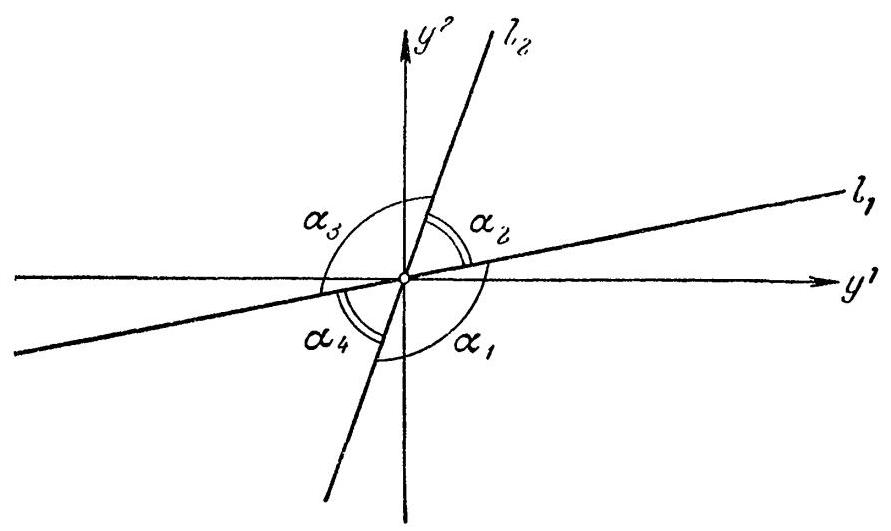
\includegraphics[max width=0.8\textwidth]{images/bo_d547imjef24c73bgfcdg_174_313_409_891_531_0.jpg}
\end{center}
\hspace*{3em}

Pnc. 53.

рис. 54. Вспоминая характер изменения величин у и и, у, мы приходим к следующему выводу относительно опти- мальных управлений. Если начальное значение фо векто- ра ф = (ψ1, ψ2) расположено внутри четвертого квадранта

\begin{center}
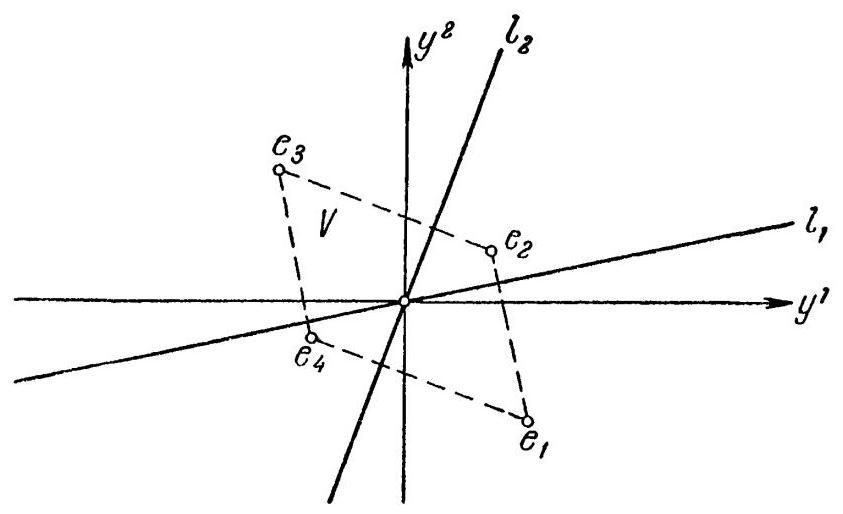
\includegraphics[max width=0.7\textwidth]{images/bo_d547imjef24c73bgfcdg_174_341_1271_843_514_0.jpg}
\end{center}
\hspace*{3em}

Pnc. 54.

(или на его сторонах), то при дальнейшем своем измене- нии вектор ф не выйдет из этого квадранта, т. е. будет все время находиться внутри угла α,. Следовательно, мы будем все время иметь \(v = {e}_{1}\) (без переключений). Этому управлению соответствует траектория системы (56), оканчивающаяся в начале координат (рис. 55). Анало- гично, если начальное значение \({\psi }_{0}\) вектора \(\psi\) находится внутри или на сторонах второго квадранта, то мы будем иметь \(v = {e}_{3}\) в течение всего движения, т. е. получим траекторию системы (56)3, оканчивающуюся в начале

Итак, пусть вектор цо рас- положен внутри первого коорди- натного угла, но одновременно лежит в угле α,. С течением вре- мени вектор ф монотонно по- координат (рис. 56). Все осталь- ные оптимальные траектории со- ответствуют случаям, когда век- тор фо расположен внутри первого или третьего квадрантов. Мы рассмотрим случай, когда цо ле- жит внутри первого квадранта (случай третьего квадранта полу- чается при помощи симметрии относительно начала координат). ворачивается против часовой стрелки, приближаясь к оси ординат. Следовательно, оптимальное управление имеет два переключения: сначала v = e1, за- тем, после первого переключения, \(v = {e}_{2}\) и,наконец,после второго переключения, \(v = {e}_{3}\). Мы сейчас покажем,что при наличии указан- ных двух переключений проме- жуток времени, в течение кото- poro управляющий параметр у принимает значение \({e}_{2}\),шмеет вполне определенную д л и н у (независимо от выбора начальных условий). В самом де- ле, обозначим угловые коэффици- енты прямых и и и и состовет- ственно через \({k}_{1},{k}_{2}\) (где \({k}_{1} < {k}_{2}\), см. рис. 53). Так как изменение вектора ф описывается формулами

\[
{\psi }_{1} = {c}_{1}{e}^{-{\lambda }_{1}t},\;{\psi }_{2} = {c}_{2}{e}^{-{\lambda }_{2}t}
\]

\begin{center}
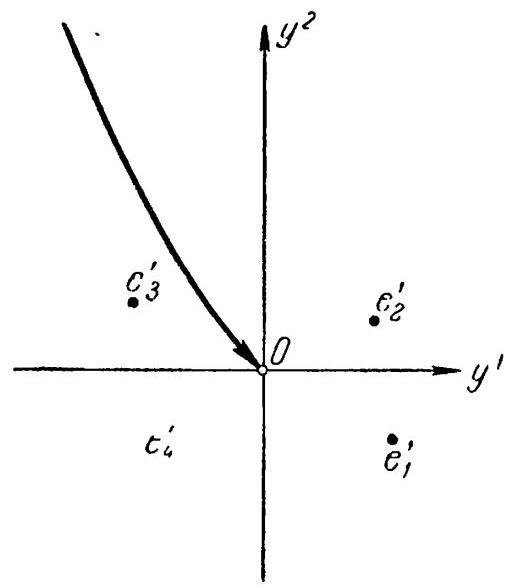
\includegraphics[max width=0.4\textwidth]{images/bo_d547imjef24c73bgfcdg_175_104_398_516_588_0.jpg}
\end{center}
\hspace*{3em}

Pac. 55.

\begin{center}
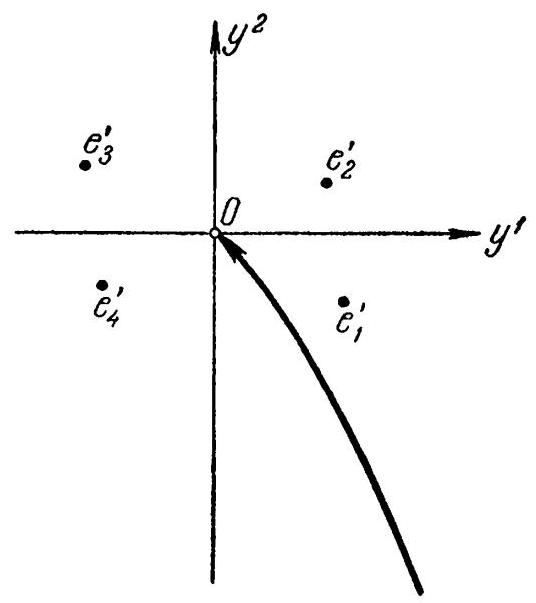
\includegraphics[max width=0.4\textwidth]{images/bo_d547imjef24c73bgfcdg_175_879_1221_536_603_0.jpg}
\end{center}
\hspace*{3em}

Prac. 56

(где \({c}_{1} > 0\) и где > 0,так как вектор ψ расположен в пер- вом квадранте), то момент переключения \({\tau }_{1}\) из вершины

\({e}_{1}\) в вершину \({e}_{2}\) (т. e. момент перехода вектора ф через прямую \({l}_{1}\) ) определяется из соотношения

\[
\frac{{c}_{2}{e}^{-{\lambda }_{2}{\tau }_{1}}}{{c}_{1}{e}^{-{\lambda }_{1}{\tau }_{1}}} = {k}_{1}.
\]

Аналогично, момент переключения \({\tau }_{2}\) из вершины \({e}_{2}\) в вершину \({e}_{3}\) (т. e. момент перехода вектора ф через пря- мую \({l}_{2}\) ) определяется из соотношения

\[
\frac{{c}_{2}{e}^{-{\lambda }_{2}{\tau }_{2}}}{{c}_{1}{e}^{-{\lambda }_{1}{\tau }_{2}}} = {k}_{2}.
\]

Takuu o6pa30M,

\[
{\tau }_{1} = \frac{1}{{\lambda }_{1} - {\lambda }_{2}}\ln \frac{{k}_{1}{c}_{1}}{{c}_{2}},\;{\tau }_{2} = \frac{1}{{\lambda }_{1} - {\lambda }_{2}}\ln \frac{{k}_{2}{c}_{1}}{{c}_{2}},
\]

и потому отрезок времени [1, т, 2], в течение которого управляющий параметр у принимает значение е, имеет длину

\[
{\tau }_{2} - {\tau }_{1} = \frac{1}{{\lambda }_{1} - {\lambda }_{2}}\left( {\ln \frac{{k}_{2}{c}_{1}}{{c}_{2}} - \ln \frac{{k}_{1}{c}_{1}}{{c}_{2}}}\right)  = \frac{1}{{\lambda }_{1} - {\lambda }_{2}}\ln \frac{{k}_{2}}{{k}_{1}}. \tag{58}
\]

Число, стоящее в правой части соотношения (58), не за- висит от си и с (т. е. от начального значения фо вектора \(\psi )\), и мы обозначим его через T.

Итак, при изменении вектора ф в первом квадранте оптимальные управления имеют следующий вид. Управ- ляющий параметр у в течение некоторого времени при- нимает значение \(v = {e}_{1}\),Затем в течение времени Тпара- метр у принимает значение у е ее, после чего вплоть до окончания движения он принимает значение v = e,

Разумеется, число переключений может оказаться и меньшим, чем два. Например, мы могли бы начать рассмо- трение движения в момент, когда управляющий параметр \(v\) уже принял значение ее. Тогда мы получили бы, что пара- метр и в течение времени, н в п р е в о c x о д я щ е г о 7, находится в вершине \({e}_{2}\), после чего переключается в вер- шину \({e}_{3}\). Точно так же могло бы оказаться, например, что движение закончилось (попаданием в начало координат) до момента переключения из вершины е, в вершину \({e}_{3}\). Иначе говоря, если управляющий параметр у совершает меньше двух переключений, то время пребывания его в вершине е в не превосходит \(T\) (причем переключе- ние может происходить либо из вершины \({e}_{1}\) в вершину \({e}_{2}\), либо из е, в х. п

Теперь уже нетрудно построить на плоскости π «ли- нии переключения», определяющие синтез оптимальных управлений. Наметим сначала траектории, соответствую- щие д в ум переключениям. Заключительный этап движе- ния на таких траекториях соответствует значению па- раметра v=e, т. е. движе- ние происходит по дуге АО траектории системы \({\left( {56}\right) }_{3}\), оканчивающейся в начале координат (рис. 56). Перед попаданием на линию АО движение происходило в силу системы \({\left( {56}\right) }_{2}\). Таким обра- 30M, \({AO}\) есть линия переклю- чения из вершины е в вер- шину \({e}_{3}\). Пусть \(X\) — некоторая точка линии АО. Тогда пред- шествующий точке \(X\) уча- сток YX оптимальной траек- тории представляет собой дугу траектории системы (56), соответствующую отрезку времени Т (рис. 57). Так как решения системы (57) имеют вид у 1 сп.нс или \({y}^{2} = {c}_{2}{e}^{{\lambda }_{2}t}\), to в результате движения точки по траектории этой системы в течение времени 7 ее абсцисса умножает- ся на \({e}^{{\lambda }_{1}T}\), a ордината — на \({e}^{{\lambda }_{2}T}\). Система же \({\left( {56}\right) }_{2}\) отли- чается от системы (57) только сдвигом положения равно- весия. Таким образом, точки X получаются из соответствую- щих точек Y (рис. 57) с помощью аффинного преобразования \(L\), которое в системе координат с началом в точке е (55)) и осями, параллельными осям у 1, у 2, заключается в умножении абсциссы на \({e}^{{\lambda }_{1}T}\), a ординаты - на \({e}^{{\lambda }_{2}T}\). Следовательно, геометрическое место точек Y представляет собой линию \({CB}\), переходящую в линию \({AO}\) при аффин- ном преобразовании L (рис. 5в). Наметив еще линию ВО, представляющую собой дугу траектории системы (56)2, оканчивающуюся в начале координат и соответствующую отрезку времени \(T\),мы найдем,что вся «полоса» \({AOBC}\) за- полнена кусками траекторий системы (56)2, начинающимися на линии СВ, кончающимися на линии АО и соответствую- щими отрезку времени \(T\).

\begin{center}
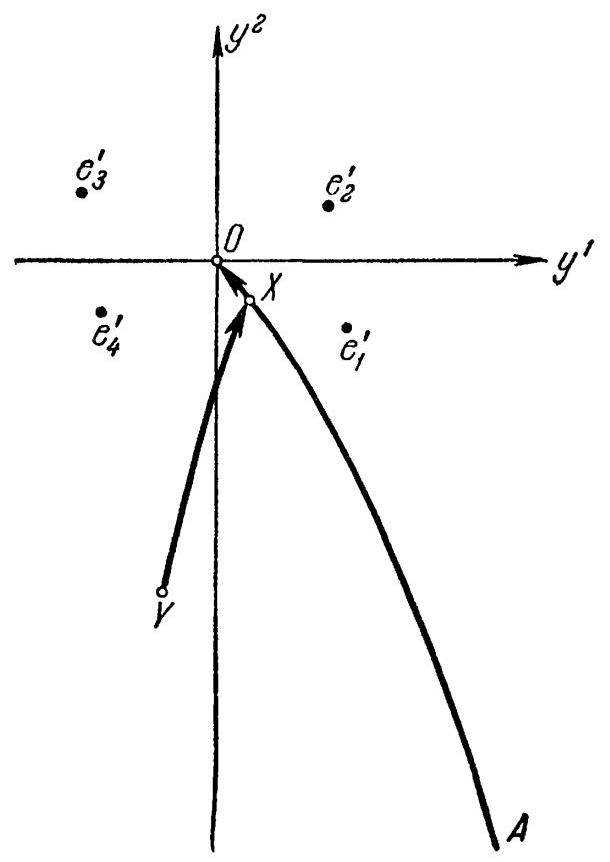
\includegraphics[max width=0.5\textwidth]{images/bo_d547imjef24c73bgfcdg_177_104_510_610_862_0.jpg}
\end{center}
\hspace*{3em}

Pac. 57.

\begin{center}
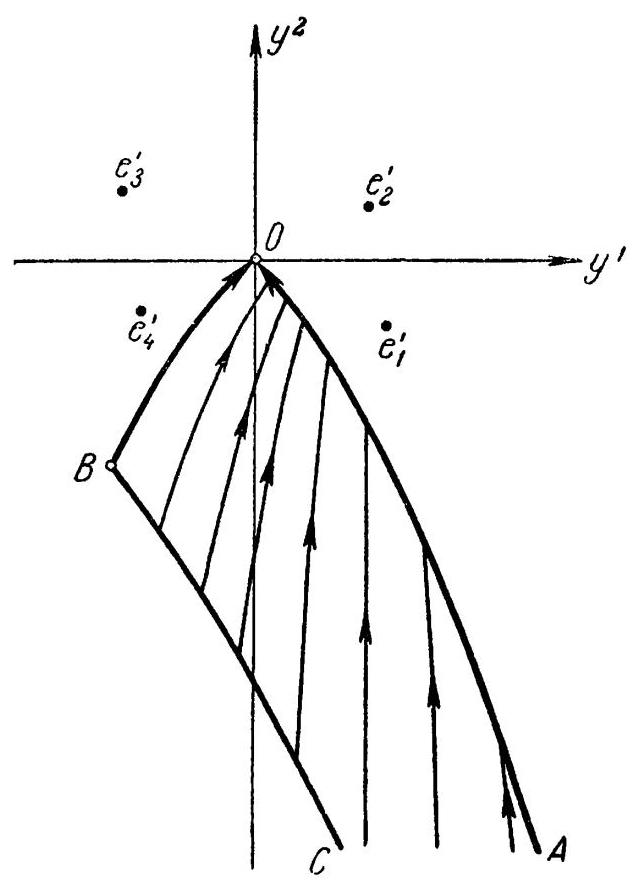
\includegraphics[max width=0.5\textwidth]{images/bo_d547imjef24c73bgfcdg_178_781_442_637_886_0.jpg}
\end{center}
\hspace*{3em}

Рис. 58.

Итак, геометрическим ме- CTOM ТОЧеК \(Y\),в которых происходит переключение из вершины \({e}_{1}\) в вершину \({e}_{2}\), служит линия СВ. До точки \(Y\) движение совершалось по траектории системы (56)1. В результате мы получаем траектории, соответствую- щие д в у м переключениям (рис. 59). «Крайняя» траек- тория DBO на рис. 59 соот- ветствует о д н о м у перек- лючению — фазовая точка по- падает в начало координат как раз в тот момент, когда должно было бы произой- ти второе переключение (из вершины \({e}_{2}\) в вершину \({e}_{3}\) ).

Рассмотрим теперь траектории, соответствующие одно- му переключению из вершины \({e}_{1}\) в вершину \({e}_{2}\). Заклю- чительный этап движения происходит в этом случае по траектории системы (56), в течение времени, не прево- сходящего \(T\), \(\mathbf{u}\) оканчивается в начале координат, \(\mathbf{T}\). e. происходит по некоторой части ZO линии BO (рис. 6O). До точки Z движение происходило в силу системы (56). Когда точка Z пробегает всю дугу BO, траектории ука- занного вида заполняют «полосу» DBOA' (рис. 61), где \({A}^{\prime }O -\) траектория системы (56)1, оканчивающаяся в на- чале координат.

Объединяя все полученные оптимальные траектории, мы находим, что вся часть плоскости слева от линии \({AO}{A}^{\prime }\) заполняется ими (рис. 5,9,61). Очевидно, что линия \({A}^{\prime }O\) симметрична линии АО относительно начала координат.

Справа от линии АОА' поведение траекторий симмет- рично, а переключения происходят из вершины ез в вер- шину \({e}_{4}\), a затем в е, В результате синтез оптимальных

\begin{center}
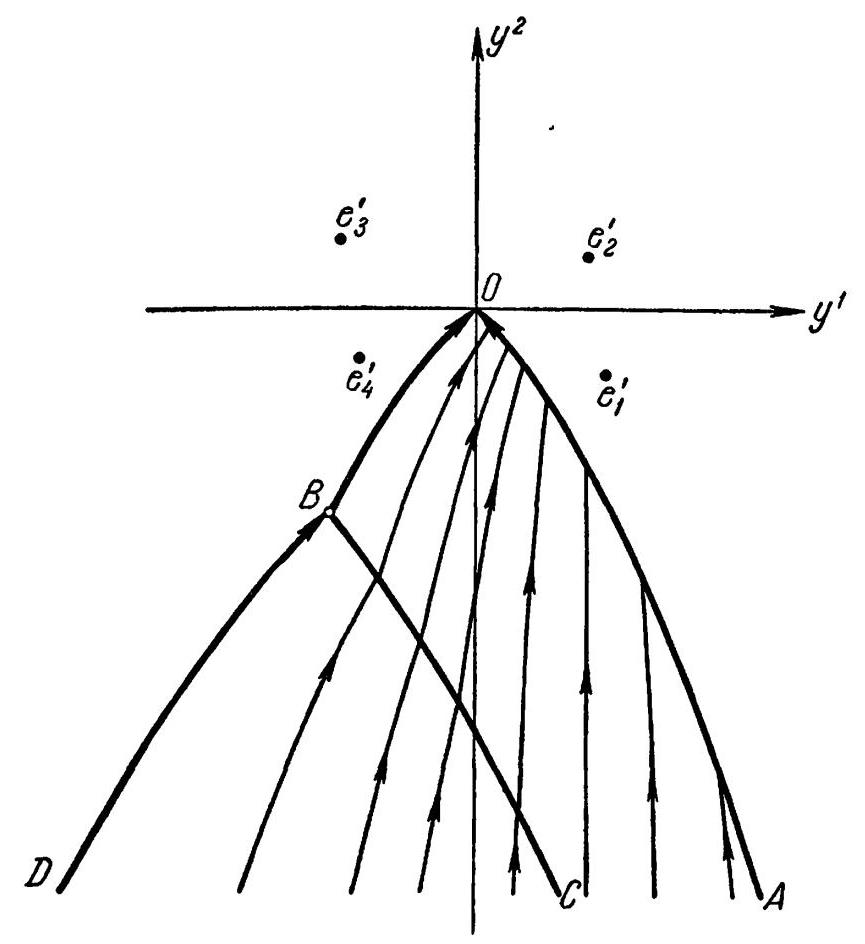
\includegraphics[max width=0.7\textwidth]{images/bo_d547imjef24c73bgfcdg_179_331_400_865_944_0.jpg}
\end{center}
\hspace*{3em}

Pac. 59.

\begin{center}
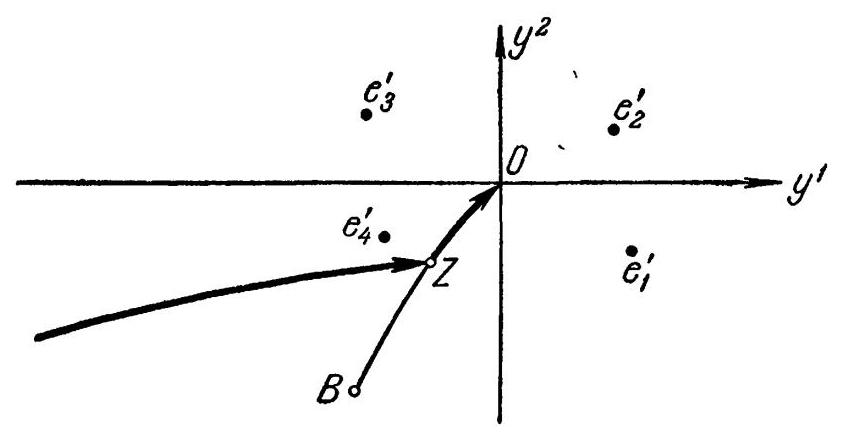
\includegraphics[max width=0.7\textwidth]{images/bo_d547imjef24c73bgfcdg_179_340_1469_842_432_0.jpg}
\end{center}
\hspace*{3em}

Prac. 60.

управлений осуществляется во всей плоскости (рис. 6). Вид оптимальных траекторий показан на рис. 63.

При переходе от переменных \({y}^{1},{y}^{2}\) к переменным \({x}^{1},{x}^{2}\) картина оптимальных траекторий аффинно искажается.

Пример 3

(Случай, когда многогранник U является одномерным, а собственные значения матрицы (а/і) действительны.)

\begin{center}
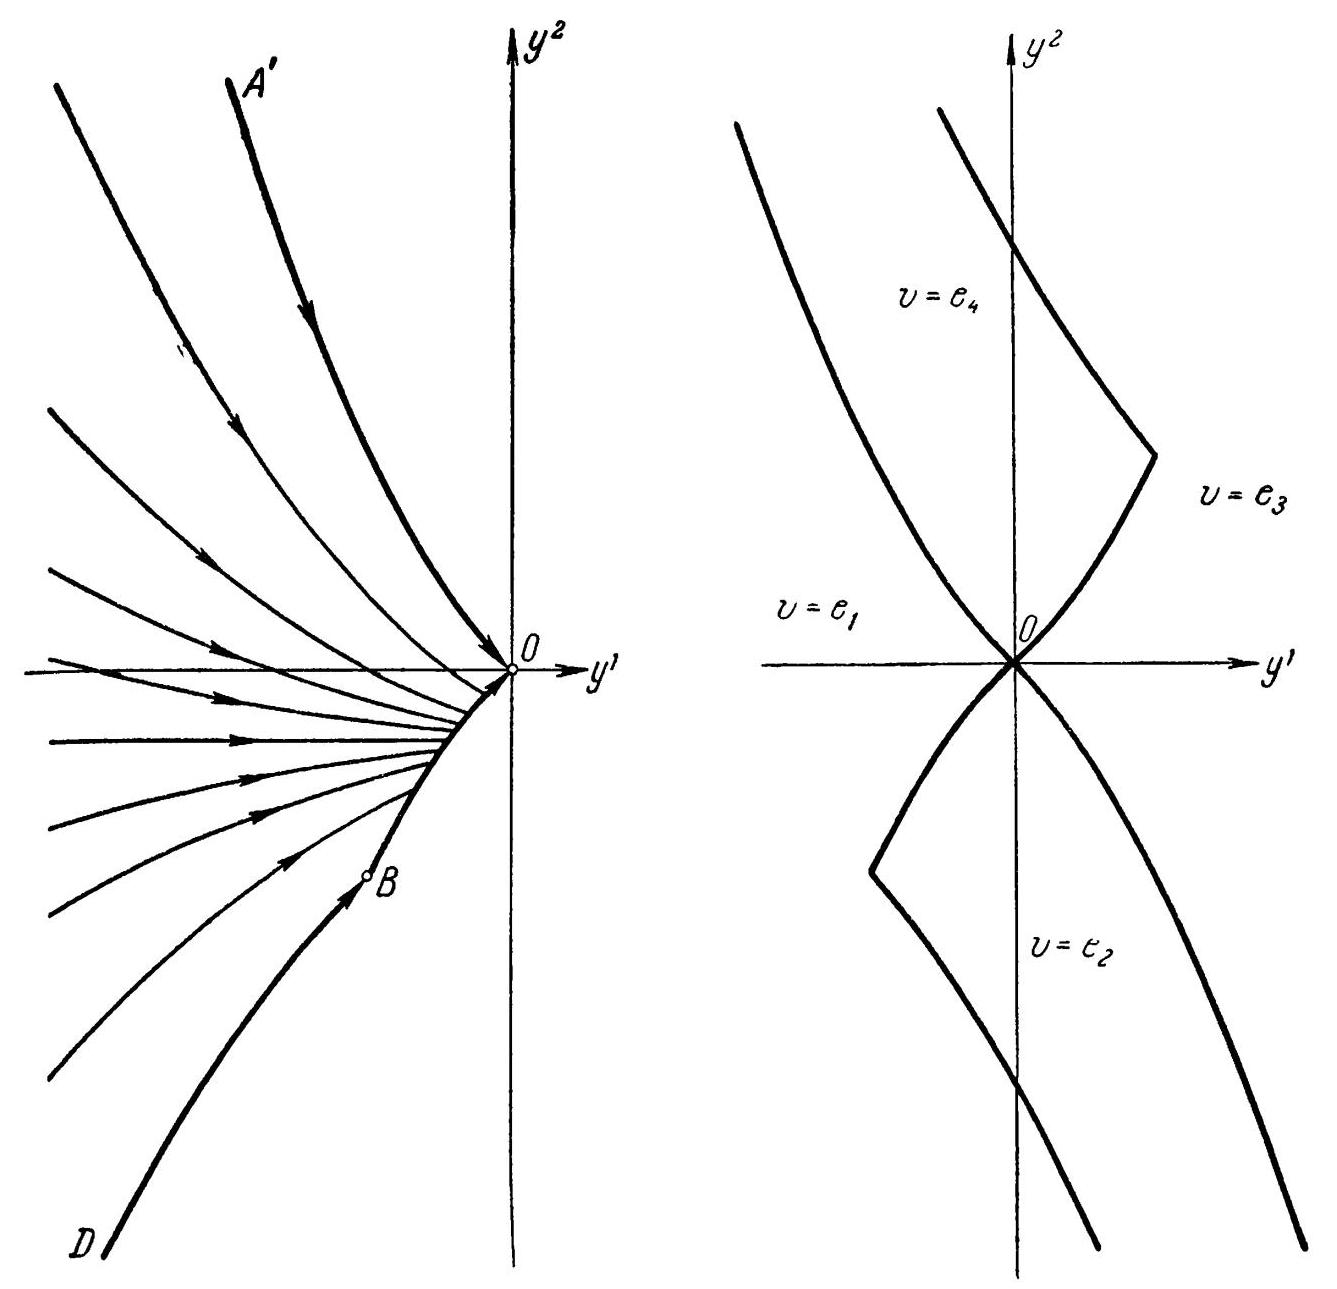
\includegraphics[max width=1.0\textwidth]{images/bo_d547imjef24c73bgfcdg_180_94_493_1337_1289_0.jpg}
\end{center}
\hspace*{3em}

Pnc. 61.

Pnc. 62.

Предположим, что в системе (1) r = 1, т. е. управляю- щий параметр и является действительным числом; пред- положим, кроме того, что это число может изме- няться в пределах —1 < и < 1. Таким образом, мно- гогранник И представляет собой в рассматриваемом

случае отрезок [ —1, 1] числовой оси, а система (1) при- нимает вид

\[
\frac{d{x}^{i}}{dt} = \mathop{\sum }\limits_{{v = 1}}^{n}{a}_{v}^{i}{x}^{v} + {b}^{i}u,\;\left| u\right|  \leq  1,i = 1,2,\ldots ,n. \tag{59}
\]

Предположим, наконец, что собственные значения матрицы

\begin{center}
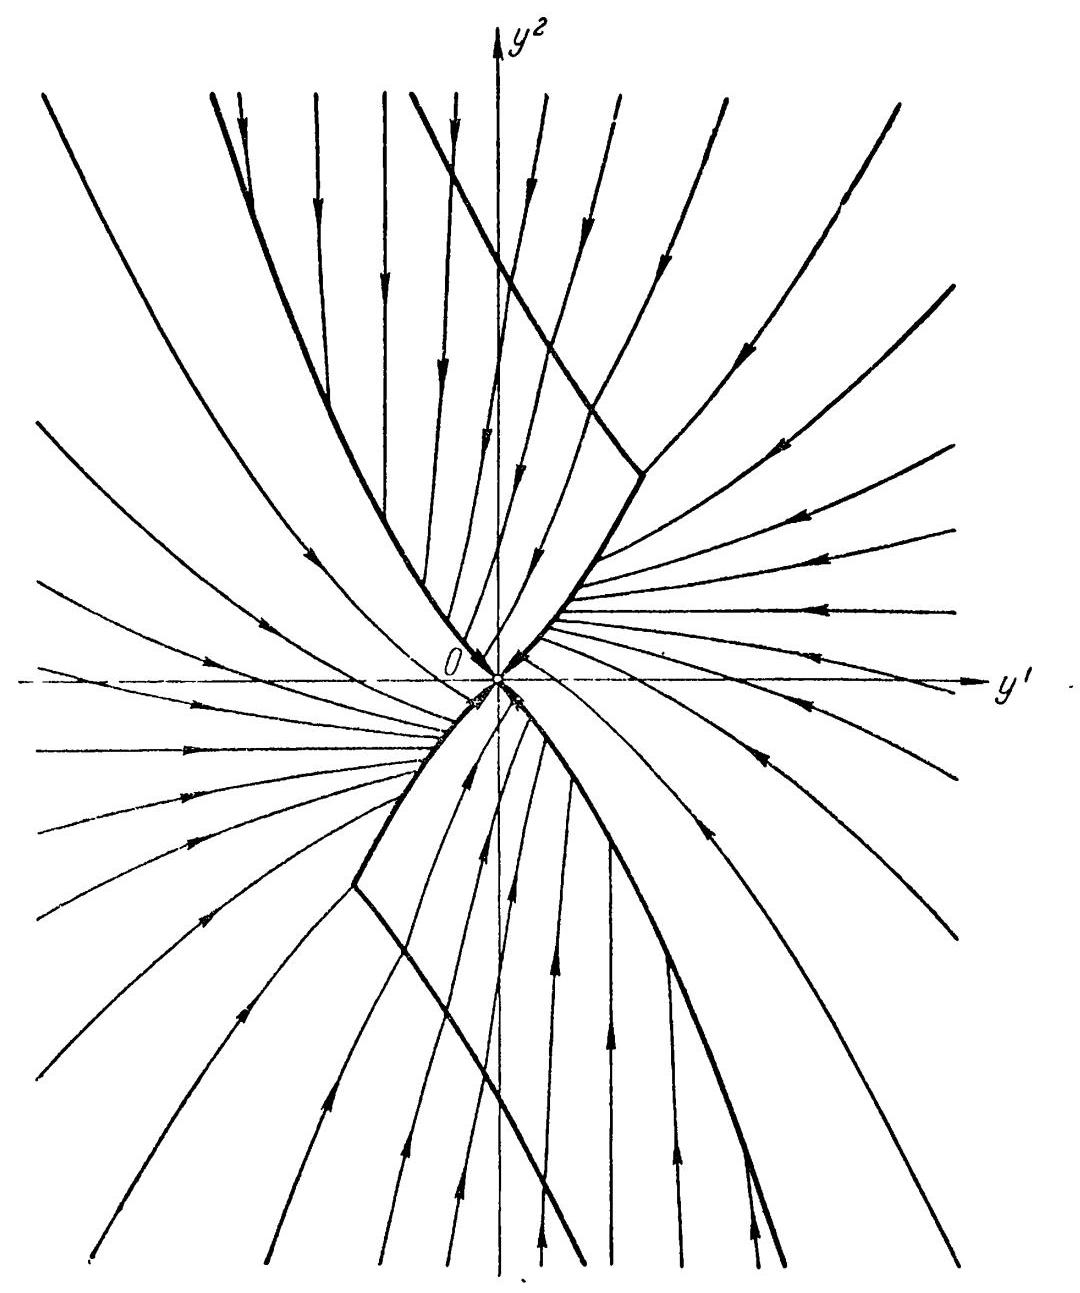
\includegraphics[max width=1.0\textwidth]{images/bo_d547imjef24c73bgfcdg_181_232_572_1080_1293_0.jpg}
\end{center}
\hspace*{3em}

Pac. 63.

\(\left( {a}_{j}^{i}\right)\) действительны. Тогда, согласно теореме 10, оптималь- ное управление содержит не более n интервалов постоян- ства, причем на этих интервалах поочередно и = + 1 и \(u =  - 1\) .

Иначе говоря, на каждом интервале постоянства движение происходит в силу одной из двух следующих CIICTEM:

\[
\frac{d{x}^{i}}{dt} = \mathop{\sum }\limits_{{v = 1}}^{n}{a}_{v}^{i}{x}^{v} + {b}^{i},i = 1,2,\ldots ,n, \tag{60}
\]

\[
\frac{d{x}^{i}}{dt} = \mathop{\sum }\limits_{{v = 1}}^{n}{a}_{v}^{i}{x}^{v} - {b}^{i},i = 1,2,\ldots ,n. \tag{60}
\]

Обозначим через \({M}_{n}^{ + }\) траекторию системы (60), окан- чивающуюся в начале координат, а через Мг — траекторию системы (60)\_, оканчивающуюся в начале координат.

\begin{center}
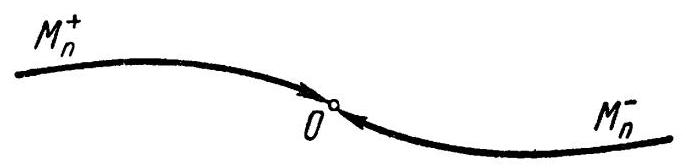
\includegraphics[max width=0.6\textwidth]{images/bo_d547imjef24c73bgfcdg_182_415_875_686_168_0.jpg}
\end{center}
\hspace*{3em}

Pac. 64.

Вместе \({M}_{n}^{ + }\) и \({M}_{n}^{ - }\) составляют проходящую через начало координат линию, которую мы обозначим через \({M}_{n}\) (рис. 64). В силу сказанного выше о характере оптималь- ных управлений ясно, что заключительный этап опти- мального движения (завершающийся попаданием в нача- ло координат) представляет собой движение по линии \({M}_{n}^{ + }\) или \({M}_{n}^{ - }\).

\begin{center}
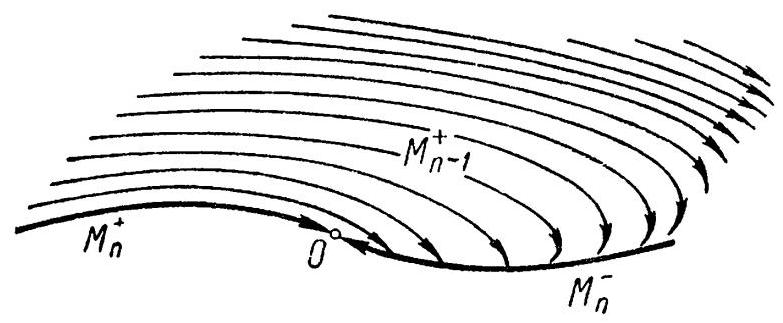
\includegraphics[max width=0.7\textwidth]{images/bo_d547imjef24c73bgfcdg_182_367_1343_783_323_0.jpg}
\end{center}
\hspace*{3em}

Prac. 65.

Рассмотрим теперь всевозможные траектории системы (60), оканчивающиеся в точках линии М- (рис. 65). Эти траектории заполняют некоторую поверхность \({M}_{n - 1}^{ + }\),имею- щую в качестве своего края линию М„ Аналогично, траектории системы (60)\_, оканчивающиеся в точках линии \({\bar{M}}_{n}^{ + }\), заполняют некоторую поверхность \({M}_{n - 1}^{ - }\), имеющую в качестве своего края линию \({M}_{n}\). Объединив \({M}_{n - 1}^{ * }\) и \({M}_{n - 1}^{ - }\) вместе, мы получаем поверхность, которую обозначим через \({M}_{n - 1}\) (puc. 66). Ясно, что последние два этапа всякого оптимального движения совершаются по поверх- ности \({M}_{n - 1}\), ибо только по траекториям этой поверхности можно попасть на линию \({M}_{n}\), по которой совершается заключительный этап движения.

\begin{center}
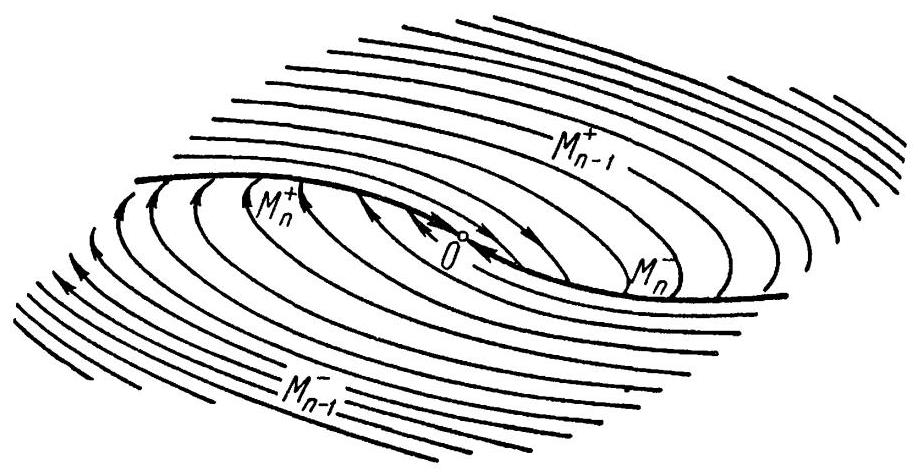
\includegraphics[max width=0.8\textwidth]{images/bo_d547imjef24c73bgfcdg_183_303_739_918_472_0.jpg}
\end{center}
\hspace*{3em}

Puc. 66.

Далее, траектории системы (60), оканчивающиеся в точках поверхности \({M}_{n - 1}^{ - }\), образуют трехмерное много- образие \({M}_{n - 2}^{ + }\),краем которого служит поверхность \({M}_{n - 1}\). Траектории системы (60), оканчивающиеся в точках поверхности \({M}_{n - 1}^{ + }\), образуют трехмерное многообразие \({M}_{n - 2}^{ - }\) c краем \({M}_{n - 1}\). Вместе \({M}_{n - 2}^{ + }\) u \({M}_{n - 2}^{ - }\) образуют трех- мерное многообразие \({M}_{n - 2}\),в котором совершаются послед- ние три этапа всякого оптимального движения.

Продолжая таким образом, мы построим многообразия \({M}_{n},{M}_{n - 1},\ldots,{M}_{1}\),причем многообразие \({M}_{i}\) имеет раз- мерность \(n - i + 1\). Многообразие \({M}_{i + 1}\) расположено цели- ком в многообразии М, и разбивает это многообразие на две области \({M}_{i}^{ + }\) и При этом область М; образо- вана всевозможными траекториями системы (60), оканчи- вающимися на \({M}_{{\bar{i}}_{+1}}\), a область \({M}_{\iota }^{ - }\) образована всевоз- можными траекториями системы (60), оканчивающимися на \({M}_{i + 1}^{ + }\). Последнее многообразие \({M}_{1}\) либо совпадает со всем фазовым пространством Х, либо представляет собой некоторую область этого пространства, содержащую нача- ло координат. Внутри этой области М1 и осуществляется синтез оптимальных управлений.

Этот синтез осуществляется следующим образом: во всех областях М’ управляющий параметр и принимает значение +1, а во всех областях М 7 он принимает зна- чение —1. Фазовая точка двигается в области М1, при- чем \(u =  + 1\), если она находится в \({M}_{1}^{ + }\) и \(u =  - 1\), если она находится в М-. В момент попадания на многообра- зие \({M}_{2}\) происходит переключение, и все дальнейшее движение совершается по многообразию \({M}_{2}\). Следующий момент переключения наступает тогда, когда точка, двигаясь по \({M}_{2}\), попадает на многообразие \({M}_{3}\). После этого точка продолжает двигаться по Мз и т. д. Заклю- чительный этап движения, завершающийся попаданием в начало координат, происходит по линии М„ Таким образом, всего за время движения происходит n — 1 пе- реключений. Разумеется, при некоторых начальных поло- жениях фазовой точки число переключений может ока- заться и меньшим, чем л — 1 (например, может оказаться, что точка \({x}_{0}\) расположена на многообразии \({M}_{2}\),или же на многообразии \({M}_{3}\) и т. п.).

Пример 1 в § 5 является частным случаем указан- ного общего построения.

\section*{Пример 4}

Поставим следующую задачу. В n-мерном евклидовом пространстве движется управляемая точка, причем «дви- гатель» ее может сообщать этой точке ускорение, не пре- восходящее по модулю единицы и направленное в любую сторону. Как следует управлять движением этой точки, чтобы, имея заданное начальное положение и заданную начальную скорость, она за кратчайшее время попала в начало координат (с произвольной конечной ско- ростью)?

Для решения этой задачи обозначим координаты дви- жущейся точки через \({x}^{1},{x}^{2},\ldots,{x}^{n}\), компоненты ее скорости — через \({x}^{n + 1},\ldots,{x}^{2n}\), a компоненты ускорения — через \({u}^{1},\ldots,{u}^{n}\). Maccy точки примем равной единице. Тогда уравнения движения точки запишутся в виде

\[
\left. \begin{aligned} \frac{d{x}^{1}}{dt} &  = {x}^{n + 1}, \\  \frac{d{x}^{2}}{dt} &  = {x}^{n + 2}, \\  \ldots & \ldots \\  \frac{d{x}^{n + 1}}{dt} &  = {x}^{2n}, \\  \frac{d{x}^{n + 1}}{dt} &  = {u}^{1}, \\  \frac{d{x}^{2n}}{dt} &  = {u}^{2}, \\  \ldots & \ldots \\  \frac{d{x}^{2n}}{dt} &  = {u}^{n}, \end{aligned}\right\} \tag{61}
\]

Так как ускорение и = (и'..., и") должно по модулю не превосходить единицы, то область управления И опре- деляется неравенством

\[
{\left( {u}^{1}\right) }^{2} + {\left( {u}^{2}\right) }^{2} + \ldots  + {\left( {u}^{n}\right) }^{2} \leq  1. \tag{62}
\]

Далее, так как начальное положение и начальная ско- рость точки заданы, то в фазовом пространстве X пере- менных \({x}^{1},{x}^{2},\ldots,{x}^{n},\ldots,{x}^{2n}\) задано начальное поло- жение \({x}_{0} = \left( {{x}_{0}^{1},\ldots,{x}_{0}^{2n}}\right)\). Треóование попадания в начало координат (с произвольной конечной скоростью) означает, что в конечный момент движения должны быть выполне- ны соотношения

\[
{x}^{1} = {x}^{2} = \ldots  = {x}^{n} = 0, \tag{63}
\]

а величины хгч, …, \({x}^{2n}\) могут быть произвольными. Иначе говоря, задача заключается в быстрейшем попа- дании объекта, управляемого уравнениями (61), (62), из начальной точки \({x}_{0} \in  X\) в какую-либо точку многообра- зия \({S}_{1}\), определяемого в X уравнениями (63). Многооб- разие \({S}_{1}\) представляет собой, очевидно, n-мерную плос- кость.

Функция H имеет в рассматриваемом случае следую- щий вид:

\[
H = {\psi }_{1}{x}^{n + 1} + {\psi }_{2}{x}^{n + 2} + \ldots  + {\psi }_{n}{x}^{2n} + {\psi }_{n + 1}{u}^{1} + \ldots  + {\psi }_{2n}{u}^{n};(6 \tag{64}
\]

с помощью этой функции находим систему уравнений для вспомогательных переменных ц.:

\[
\frac{d{\psi }_{1}}{dt} = 0
\]

\[
\frac{d{\psi }_{2}}{dt} = 0
\]

.......

\[
\frac{d{\psi }_{n}}{dt} = 0
\]

\[
\frac{d{\psi }_{n + 1}}{dt} =  - {\psi }_{1}
\]

\[
\frac{d{\psi }_{n + 2}}{dt} =  - {\psi }_{2}
\]

\[
\frac{d{\psi }_{2n}}{dt} =  - {\psi }_{n}
\]

Из этой системы вытекает, что в течение всего опти- мального движения величины \({\psi }_{1},{\psi }_{2},\ldots,{\psi }_{n}\) сохраняют постоянные значения, и потому величины \({\psi }_{n + 1},{\psi }_{n + 2},\ldots\)..., \({\psi }_{2n}\) являются линейными функциями времени.

Напишем теперь условие трансверсальности в правом конце оптимальной траектории. Для того чтобы вектор \(\psi  = \left( {{\psi }_{1},\ldots,{\psi }_{n},{\psi }_{n + 1},\ldots,{\psi }_{2n}}\right)\) был ортогонален к много- образию \({S}_{1}\), определяемому уравнениями (63), оиевидно, необходимо и достаточно выполнение условий

\[
{\psi }_{n + 1} = {\psi }_{n + 2} = \ldots  = {\psi }_{2n} = 0.
\]

Таким образом, условие трансверсальности в правом кон- це оптимальной траектории имеет вид

\[
{\psi }_{n + 1}\left( {t}_{1}\right)  = {\psi }_{n + 2}\left( {t}_{1}\right)  = \ldots  = {\psi }_{2n}\left( {t}_{1}\right)  = 0, \tag{65}
\]

где \({t}_{1}\) - момент попадания фазовой точки на многообра- зие \({S}_{1}\). Вспоминая теперь,что функции \({\psi }_{n + 1},{\psi }_{n + 2},\ldots,{\psi }_{2n}\) линейны, мы находим из (65), что имеют место формулы

\[
{\psi }_{n + 1} = {a}_{1}\left( {{t}_{1} - t}\right) ,\;{\psi }_{n + 2} = {a}_{2}\left( {{t}_{1} - t}\right) ,\ldots ,\;{\psi }_{2n} = {a}_{n}\left( {{t}_{1} - t}\right) ,
\]

(66)

где \({a}_{1},{a}_{2},\ldots,{a}_{n} -\) постоянные величины. Так как вели- чины ψ, определены лишь с точностью до общего поло- жительного множителя пропорциональности, то мы можем при этом предполагать, что вектор \(a = \left( {{a}_{1},{a}_{2},\ldots,{a}_{n}}\right)\) является единичным, т. е.

\[
{\left( {a}_{1}\right) }^{2} + {\left( {a}_{2}\right) }^{2} + \ldots  + {\left( {a}_{n}\right) }^{2} = 1.
\]

Подставляя найденные значения (66) в формулу (64), мы получаем

\[
H = \ldots  + \left( {{t}_{1} - t}\right) \left( {{a}_{1}{u}^{1} + {a}_{2}{u}^{2} + \ldots  + {a}_{n}{u}^{n}}\right) ,
\]

где многоточием обозначены члены, не зависящие от \({u}^{1},\ldots,{u}^{n}\). Так как \({t}_{1} - t > 0\) (ибо и — по след н и й момент движения), то условие максимума функции \(H\) означает, что в течение всего движения величина

\[
{a}_{1}{u}^{1} + {a}_{2}{u}^{2} + \ldots  + {a}_{n}{u}^{n} = \left( {a,u}\right)
\]

должна быть максимальной, а это, в силу (62), озна- чает, что \(u\left( t\right)  \equiv  a\), т. e. что величины \({u}^{1},{u}^{2},\ldots,{u}^{n}\) в тече- ние всего движения сохраняют постоянные значения \({u}^{i} = {a}_{i},i = 1,\ldots,n.\)

Итак, в рассматриваемом случае оптимальность дви- жения означает, что ускорение и п о с т о я н н о и вели- чина его равна единице. Это позволяет однозначно опре- делить искомое ускорение (т. е. найти направление вектора ускорения и). В самом деле, траектория движе- ния точки в рассматриваемом евклидовом пространстве представляет собой параболу

\[
{x}^{i} = {x}_{0}^{i} + {x}_{0}^{n + i}t + {u}^{i}\frac{{t}^{2}}{2},\;i = 1,\ldots ,n,
\]

где \(u = \left( {{u}^{1},\ldots,{u}^{n}}\right)\) — постоянный вектор ускорения, рав- ный по величине единице, т. е. удовлетворяющий условию

\[
{\left( {u}^{1}\right) }^{2} + {\left( {u}^{2}\right) }^{2} + \ldots  + {\left( {u}^{n}\right) }^{2} = 1. \tag{67}
\]

Для того чтобы эта траектория прошла через начало координат, должны выполняться условия

\[
{x}_{0}^{i} + {x}_{0}^{n + i}t + {u}^{i}\frac{{t}^{2}}{2} = 0,\;i = 1,\ldots ,n. \tag{68}
\]

Соотношения (67), (68) представляют собой систему из \(n + 1\) ураsнений относительно неизвестных \({u}^{1},{u}^{2},\ldots,{u}^{n},t\), причем для t мы должны получить положительное зна- чение. В случае, если таких решений окажется несколь- ко, мы должны взять решение с н а и м е н ь ш и м поло- жительным значением t (ибо речь идет о бы с т р е й ш е м попадании в начало координат). Из (68) мы получаем

\[
{u}^{i} =  - \frac{2\left( {{x}_{0}^{i} + {x}_{0}^{n + i}t}\right) }{{t}^{2}},\;i = 1,\ldots ,n, \tag{69}
\]

и подстановка в соотношение (67) дает уравнение

\[
4\mathop{\sum }\limits_{{i = 1}}^{n}{\left( {x}_{0}^{i} + {x}_{0}^{n + i}t\right) }^{2} - {t}^{4} = 0 \tag{70}
\]

относительно неизвестного \(t\). При \(t = 0\) левая часть этого уравнения принимает значение \(4\mathop{\sum }\limits_{{i = 1}}^{n}{\left( {x}_{0}^{i}\right) }^{2} > 0\;\) (разумеется, мы считаем, что точка ( \({x}_{0}^{1},{x}_{0}^{2},\ldots,{x}_{0}^{n}\) ) не совпадает с началом координат, так как в противном случае решение опти- мальной задачи очевидно: \(t = 0\) ). При \(t \rightarrow  \infty\) левая часть уравнения (70) отрицательна. Следовательно, уравнение (70) имеет хотя бы один положительный корень. Обозна- чим через \(\tau \left( {x}_{0}\right)  = \tau \left( {{x}_{0}^{1},{x}_{0}^{2},\ldots,{x}_{0}^{n},{x}_{0}^{n + 1},\ldots,{x}_{0}^{2n}}\right)\) на n - мень ш и й положительный корень этого уравнения. Тогда из (69) мы находим искомые значения компонент ускорения

\[
{u}^{i} =  - \frac{2\left( {{x}_{0}^{i} + {x}_{0}^{n + {i\tau }\left( {x}_{0}\right) }}\right) }{{\left( \tau \left( {x}_{0}\right) \right) }^{2}}.
\]

Это и дает синтез оптимальных управлений в рассматри- ваемом случае. (Функция τ (хо), а следовательно, и функ- ции \({u}^{i}\) кусочно-непрерывны.)

\section*{§ 22. Моделирование линейных оптимальных быстродействий при помощи релейных схем}

Возвратимся снова к задаче о линейных оптимальных быстродействиях, рассмотренной в \$ 17. В силу теоремы 9 каждая экстремальная траектория (см. стр. 140), исхо- дящая в момент \({t}_{0}\) из точки \({x}_{0}\),определяется начальными значениями ψ (бо) решения ψ(t) уравнения (5). Именно, если задан произвольный отличный от нуля вектор цо, то однозначно определено решение ф (н) уравнения (5) c начальным условием ψ (бо) = ψ0. После этого, в силу теоремы 9, соотношение (6) однозначно определяет соот- ветствующее экстремальное управление и(t). Наконец, зная управление и(t), мы из уравнения (2) находим и соответствующую траекторию \(x\left( t\right)\), исходящую из точки \({x}_{0}\). Таким образом, в конечном счете экстремальная траектория \(x\left( t\right)\) однозначно определяется выбором началь- ного значения фо. Если бы нам удалось найти именно такое начальное значение \({\psi }_{0}\),что траектория \(x\left( t\right)\) п р о х о - дит через начало координат 0, то управле- ние \(u\left( t\right)\) и траектория \(x\left( t\right)\), полученные указанным выше способом, будут оптимальными. В самом деле, получен- ная траектория \(x\left( t\right)\) будет идти в этом случае из точки \({x}_{0}\) в требуемую точку \(O\),и потому оптимальное управле- ние существует (теорема 13). Это оптимальное управление единственно (теорема 11) и удовлетворяет принципу мак- симума, т. е. является экстремальным (стр. 140). Но экстремальное управление, переводящее фазовую точку. из положения \({x}_{0}\) в начало координат,также единственно (теорема 12). Таким образом, экстремальное управление, переводящее фазовую точку в начало координат, как раз и является оптимальным управлением.

Следует отметить, что вы чи с л е н и е траектории \(x\left( t\right)\), соответствующей начальному значению \({\psi }_{0}\), является довольно трудоемким. Действительно, эта задача включает в себя решение уравнения (5), нахождение функции \(u\left( t\right)\) по формуле (6) и, наконец, решение уравнения (2), что сводится к решению н е с к о л ь к и х систем дифферен- циальных уравнений с последовательным «припасовыва- нием» начальных значений (ибо функция и(t) полу- чается, вообще говоря, не постоянной, а лишь кусочно- постоянной).

Если предположить, что нахождение траектории \(x\left( t\right)\) по начальному значению фо осуществляется некоторым п р и б о р о м, то остается задача поиска начального зна- чения \({\psi }_{0}\),при котором траектория \(x\left( t\right)\) проходит через 0.

В этом параграфе, не касаясь второй задачи (задачи поиска начальных значений фо), мы укажем способ построения моделирующего устройства, позволяющего по начальному значению \% находить соответствующую экстремальную траекторию \(x\left( t\right)\). Это моделирующее устрой- ство состоит из двух линейных объектов с уравнениями (2) и (5) и некоторого числа рел ей н ы х эл ем е н - т о в, количество и схема соединения которых определяют- ся многогранником \(U\) и оператором B.

Переходим к математическому описанию указанного моделирующего устройства. Рассмотрим линейный объект, фазовые состояния которого описываются переменными \({\psi }_{1},\ldots,{\psi }_{n}\),изменяющимися по закону (5). Этот объект мы будем условно изображать так, как показано на рис. 67.

\begin{center}
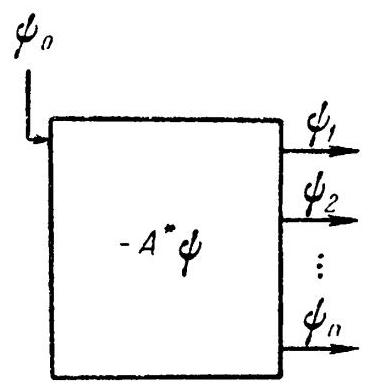
\includegraphics[max width=0.3\textwidth]{images/bo_d547imjef24c73bgfcdg_190_286_666_371_390_0.jpg}
\end{center}
\hspace*{3em}

Puc. 67.

\begin{center}
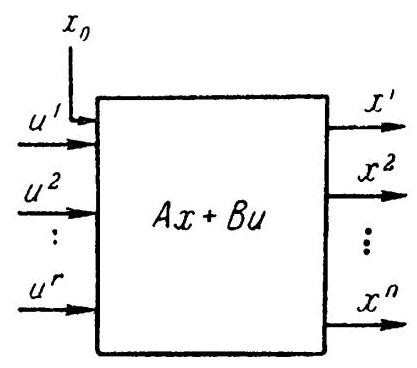
\includegraphics[max width=0.3\textwidth]{images/bo_d547imjef24c73bgfcdg_190_819_682_417_368_0.jpg}
\end{center}
\hspace*{3em}

Pnc. 68.

Задание начальных значений для величин ц. …, ф. (т. е. задание вектора фо) однозначно определяет даль- нейшее изменение величин ну,..., ф, во времени. Исход- цый объект (описываемый уравнением (2)) мы будем изображать так, как показано на рис. 68. Для того чтобы однозначно было определено изменение (во времени) вы- ходных величин (т. е. фазовых координат) \({x}^{1},\ldots,{x}^{n}\), нужно задать начальное фазовое состояние \({x}_{0}\) объекта и изменение (во времени) входных величин \({u}^{1},\ldots,{u}^{r}\) (т. е. управляющих параметров). Требуемое моделирую- щее устройство имеет вид, указанный на рис. 69; средний «ящик», помещенный между объектами, изобра- женными на рис. 67 и 68, содержит некоторое коли- чество релейных элементов. Описанию этого среднего «ящика» и посвящена остальная часть параграфа.

\begin{center}
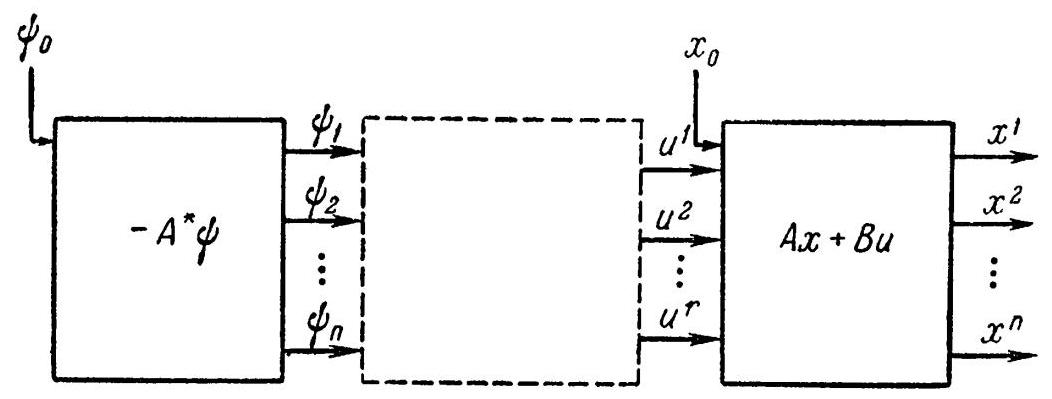
\includegraphics[max width=0.9\textwidth]{images/bo_d547imjef24c73bgfcdg_190_241_1378_1052_399_0.jpg}
\end{center}
\hspace*{3em}

Prac. 69.

Прежде всего отметим частные случаи, в кото- рых устройство среднего «ящика» особенно просто. Рассмотрим сначала случай, ког- да в уравнение (2) входит только один управляющий параметр и,

\begin{center}
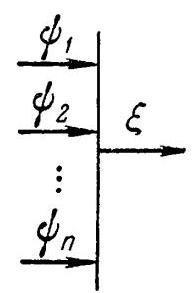
\includegraphics[max width=0.2\textwidth]{images/bo_d547imjef24c73bgfcdg_191_273_516_194_293_0.jpg}
\end{center}
\hspace*{3em}

Prac. 70

\begin{center}
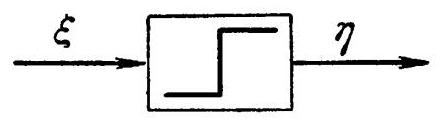
\includegraphics[max width=0.4\textwidth]{images/bo_d547imjef24c73bgfcdg_191_812_682_437_120_0.jpg}
\end{center}
\hspace*{3em}

Prac. 71.

изменяющийся в пределах — 1 ≤ u ≤ 1 (т. е. случай, когда многогранник \(U\) представляет собой отрезок [—1, 1]). В этом случае матрица (б’) превращается в с т о л б е ц \(\left( {{b}^{1},{b}^{2},\ldots,{b}^{n}}\right)\), a функция (7) имеет вид

\[
\mathop{\sum }\limits_{{\alpha  = 1}}^{n}{\psi }_{\alpha }\left( t\right) {b}^{\alpha }u
\]

Поэтому уравнение (6) имеет следуощее репение:

\[
u = \operatorname{sign}\left( {\mathop{\sum }\limits_{{\alpha  = 1}}^{n}{b}^{\alpha }{\psi }_{\alpha }\left( t\right) }\right) \tag{71}
\]

Иначе говоря, если мы введем в рассмотрение вспомога- тельную величину

\[
\xi  = \mathop{\sum }\limits_{{\alpha  = 1}}^{n}{b}^{\alpha }{\psi }_{\alpha } \tag{72}
\]

то решение уравнения (6) будет определяться формулой

\[
u = \operatorname{sign}\xi \text{ . } \tag{73}
\]

Переход от величин у,..., у, к величине ξ, опреде- ляемой формулой (72), осуществляется некоторым сум- мирующим устройством, условно изображенным на рис. 70. На рис. 71 показано условное изображение ре- лейного элемента, т. е. объекта, выходная и входная величины которого связаны соотношением \(\eta  = \operatorname{sign}\xi\).

Соединим теперь объекты, изображенные на рис. 67, 68, 70, 71, в одну схему (рис. 72). Ясно, что, каков бы ни был начальный вектор \({\psi }_{0}\),на выходе первого звена (в изображенной на рис. 72 схеме) мы получаем вели- чины \({\psi }_{1}\left( t\right),\ldots,{\psi }_{n}\left( t\right)\), составляющие решение уравне- ния (5). Эти величины в следующем звене (обведенном пунктиром) преобразуются по формулам (72), (73), так что на выходе этого звена мы получаем величину (71), являющуюся решением уравнения (6). Иначе говоря, на выходе второго звена мы получаем э к с т р е м а л ь н о е управление \(u\left( t\right)\), и потому выходные величины \({x}^{1}\left( t\right),\ldots,{x}^{n}\left( t\right)\) последнего звена будут давать соответ- ствующую экстремальную траекторию. Иначе говоря, схема, изображенная на рис. 72, при любых начальных значениях \({\psi }_{0}\), \({x}_{0}\) осуществляет движение объекта (2) с фазовыми координатами \({x}^{1},\ldots,{x}^{n}\) no соответствую- щей экстремальной траектории. Если схема, изображен- ная на рис. 72, осуществлена в виде прибора (модели- рующего устройства), то при использовании такого прибора остается нерешенной лишь задача поиска на- чального значения \%, для которого (при заданном начальном значении \({x}_{0}\) ) получаемая траектория приходит в начало координат.

\begin{center}
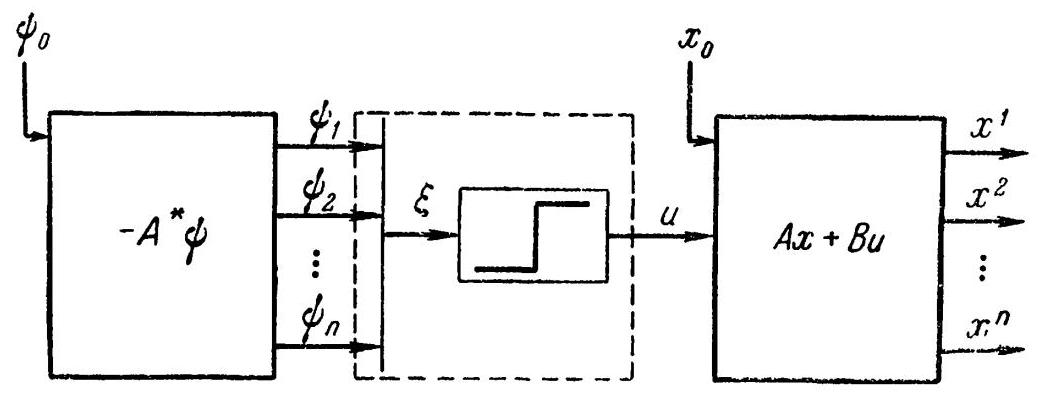
\includegraphics[max width=0.9\textwidth]{images/bo_d547imjef24c73bgfcdg_192_244_817_1043_395_0.jpg}
\end{center}
\hspace*{3em}

Pnc. 72.

Проведенные рассуждения легко обобщаются также на тот случай, когда область управления U является \(r\) -мерным кубом, т. е. определяется неравенствами

\[
\left| {u}^{i}\right|  \leq  1,\;i = 1,\ldots ,r. \tag{74}
\]

7 JI C. Понтрягин и др. В этом случае функция (7) имеет вид

\[
\mathop{\sum }\limits_{{\beta  = 1}}^{r}\mathop{\sum }\limits_{{\alpha  = 1}}^{n}{\psi }_{\alpha }\left( t\right) {b}_{\beta }^{\alpha }{u}^{\beta } \tag{75}
\]

Так как, в силу (74), область изменения каждого из управляющих параметров и",..., иг не зависит от того, какие значения приняли остальные управляющие пара- метры, то для того, чтобы функция (75) принимала максимальное значение, необходимо, чтобы к а ж д о е ee отдельное слагаемое

\[
\mathop{\sum }\limits_{{\alpha  = 1}}^{n}{\psi }_{\alpha }\left( t\right) {b}_{\beta }^{\alpha }{u}^{\beta }
\]

при \(\beta  = 1,\ldots,r\) принимало максимальное Отсюда получим

\[
{u}^{\beta } = \operatorname{sign}\left( {\mathop{\sum }\limits_{{\alpha  = 1}}^{n}{\psi }_{\alpha }\left( t\right) {b}_{\beta }^{\alpha }}\right) .
\]

Иначе говоря, если мы введем в рассмотрение вспомога- тельные величины

\[
{\xi }_{\beta } = \mathop{\sum }\limits_{{\alpha  = 1}}^{n}{b}_{\beta }^{\alpha }{\psi }_{\alpha },\;\beta  = 1,\ldots ,r, \tag{76}
\]

то решение уравнения (6) будет определяться формулами:

\[
{u}^{\beta } = \operatorname{sign}{\xi }_{\beta },\;\beta  = 1,\ldots ,r.
\]

Переход от величин ци,..., цп к величинам \({\xi }_{1},\ldots,{\xi }_{r}\) осуществляется суммирующим устройством, условно изображенным на рис. 73. Из сказанного ясно, что схема, изображенная на рис. 74, вырабатывает на выходе релейных элементов э к с т р е м а л ь н о е у п р а в - л е н и е \({u}^{1}\left( t\right),\ldots,{u}^{r}\left( t\right)\), а на выходе последнего звена — соответствующую экстремальную траекторию и(t). Отме- тим, что число релейных элементов в этой схеме равно числу управляющих параметров.

Наконец, перейдем к рассмотрению общего случая, когда многогранник \(U\) произволен. Пусть

\[
{w}_{1},{w}_{2},\ldots ,{w}_{v} \tag{77}
\]

— попарно неколлинеарные векторы, имеющие направле- ние ребер многогранника U (т. е. каждый из векторов (77) параллелен хотя бы одному ребру многогранника U и для каждого ребра имеется в системе (77) один параллельный ему вектор). Координаты вектора му будем обозначать через \({w}_{j}^{1},\ldots,{w}_{j}^{r}\). Положим

\[
{\xi }_{j} = \left( {\psi ,B{w}_{j}}\right)  = \mathop{\sum }\limits_{{\alpha  = 1}}^{n}\mathop{\sum }\limits_{{\rho  = 1}}^{r}{\psi }_{\alpha }{b}_{\rho }^{\alpha }{w}_{j}^{\rho },\;j = 1,\ldots ,\gamma . \tag{78}
\]

\({\phi }_{1}\)

Puc. 73.

\begin{center}
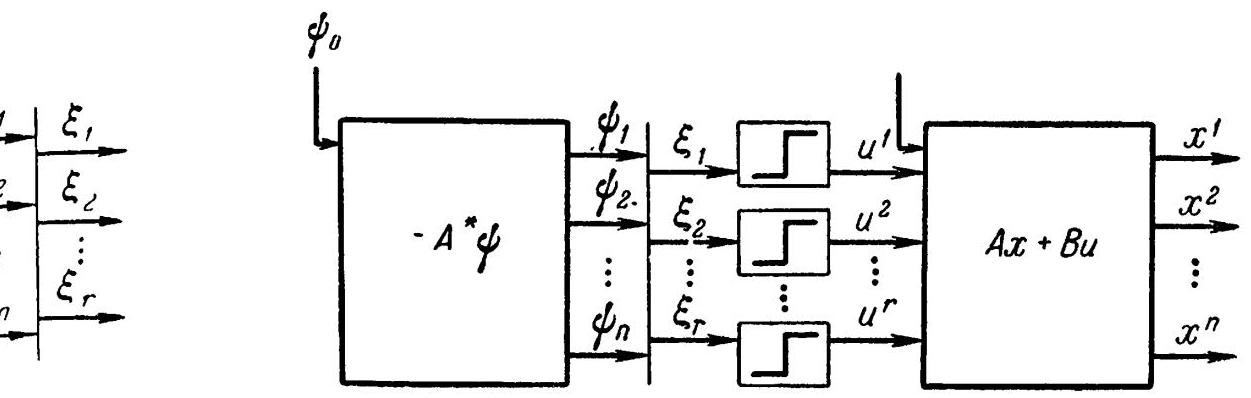
\includegraphics[max width=1.0\textwidth]{images/bo_d547imjef24c73bgfcdg_194_172_422_1251_398_0.jpg}
\end{center}
\hspace*{3em}

Pac. 74.

Таким образом, переменные \({\xi }_{1},\ldots,{\xi }_{\gamma }\) являются линей- ными формами (вообще говоря, линейно зависимыми) от

\begin{center}
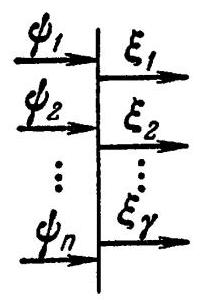
\includegraphics[max width=0.2\textwidth]{images/bo_d547imjef24c73bgfcdg_194_375_1349_203_300_0.jpg}
\end{center}
\hspace*{3em}

Pnc. 75.

\begin{center}
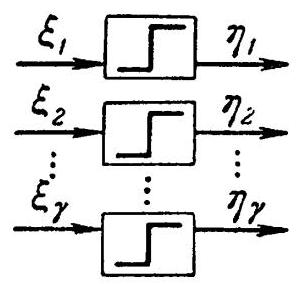
\includegraphics[max width=0.2\textwidth]{images/bo_d547imjef24c73bgfcdg_194_879_1357_300_284_0.jpg}
\end{center}
\hspace*{3em}

Prac. 76.

\({\psi }_{1},\ldots ,{\psi }_{n}\) . Переход от переменных \({\psi }_{i}\) к переменным \({\xi }_{j}\) мы будем изображать так, как показано на рис. 75. Значе- ния величин ξ, определяются величинами ψ, но обрат- ного воздействия на них не оказывают (это выражено на рис. 75 направлением стрелок).

Каждую из величин ξ, мы подадим на свой релейный элемент; выходы этих релейных элементов обозначим через \({\eta }_{1},\ldots,{\eta }_{\gamma }\) (рис. 7 6):

\[
{\eta }_{j} = \operatorname{sign}{\xi }_{j},\;j = 1,\ldots ,\gamma . \tag{79}
\]

Пусть теперь \({e}_{1},\ldots,{e}_{o}\) - все вершины многогран- ника U. Paccmotpum какую-либо одну вершину \({e}_{i}\) и пусть j — одно из чисел 1, 2,..., γ. Если исходящий из вер- шины \({e}_{i}\) вектор, равный и, идет по одному из ребер многогранника U, примыкающих к этой вершине, то мы положим \({\varepsilon }_{ij} =  + 1\). Если исходящий из вершины е, век- тор, равный — му, идет по одному из ребер многогранни- ка \(U\), примыкающих к этой вершине, то мы положим \({\varepsilon }_{ij} =  - 1\). Если же ни один из этих двух случаев места не имеет, то символ вы не определяется.

Фиксируем некоторый индекс \(i\left( { = 1,2,\ldots,q}\right)\) и будем рассматривать только такие индексы j, для которых символ \({\varepsilon }_{ij}\) определен. Тогда векторы выу (рассматри- ваемые для указанных индексов j) направлены по ребрам многогранника \(U\),исходящим из вершины \({e}_{i}\). Пусть теперь \(\psi  = \left( {{\psi }_{1},{\psi }_{2},\ldots,{\psi }_{n}}\right)\) — произвольный отличный от нуля вектор. Обозначим через В*ψ вектор простран- ства \({E}_{r}\),имеющий \(i\) -to координату \(\mathop{\sum }\limits_{{\alpha  = 1}}^{n}{b}_{i}^{\alpha }{\psi }_{\alpha },i = 1,\ldots,r\). Тогда для любого вектора и пространства E, как легко видеть, имеет место соотношение

\[
\left( {{B}^{ * }\psi ,u}\right)  = \left( {\psi ,{Bu}}\right) . \tag{80}
\]

Проведем теперь в пространстве E, гиперплоскость A, проходящую через точку \({e}_{i}\) и ортогональную вектору B*ψ, а вектор \({B}^{ * }\psi\) будем считать исходящим из точки \({e}_{i}\). Для того чтобы величина (ψ, Bu), рассматриваемая как функция точки и ∈ \(U\), достигала своего наибольшего зна- чения только в одной вершине е, необходимо и достаточно (в силу (80)), чтобы весь многогранник \(U\) находился в том полупространстве, определяемом гиперплоскостью Λ, которое не содержит вектора B*ψ, а для этого, в свою очередь, необходимо и достаточно, чтобы каждый век- тор, исходящий из точки \({e}_{i}\) и направленный по ребру многогранника U, составлял с вектором В*ψ тупой угол. Иначе говоря, для того чтобы уравнение

\[
\left( {\psi ,{Bu}}\right)  = P\left( \psi \right) \tag{81}
\]

мело единственное решение и ее ед, необходимо достаточно, чтобы все скалярные произведения

\[
\left( {{B}^{ * }\psi ,{\varepsilon }_{ij}{w}_{j}}\right)
\]

(соответствующие индексам j, для которых символ ε, определен) были отрицательными, или, иначе, чтобы были выполнены неравенства

\[
{\varepsilon }_{ij}\left( {\psi ,B{w}_{j}}\right)  < 0.
\]

В силу (78) последнее неравенство принимает вид

\[
{\varepsilon }_{ij}{\xi }_{j} < 0\text{ . } \tag{82}
\]

Итак, для того чтобы уравнение (81) имело единствен- ное решение \(u = {e}_{i}\),необходимо и достаточно, чтобы для всех j (для которых символ 8,1 определен) выполнялось неравенство (82), или, что то же самое, равенство

(см. (79)).

\[
{\varepsilon }_{ij}{\eta }_{j} =  - 1 \tag{83}
\]

Положим теперь

\[
{\zeta }_{i} = {l}_{i} - 1 + \mathop{\sum }\limits_{j}{\varepsilon }_{ij}{\eta }_{j},\;i = 1,2,\ldots ,q, \tag{84}
\]

где \({l}_{i}\) - число ребер многогранника \(U\),примыкающих к вершине \({e}_{i}\), a суммирование распространено на все значе- ния \(j\),для которых символ 8, i определён (так что в этой сумме имеется \({l}_{i}\) слагаемых). Пере- ход от величин η; к величинам \({\zeta }_{i}\) показан на рис. 77. Величина ζ, принимает значение — 1, если для всех j выполнено равенство (83), и п о л о ж и т е л ь н о е значение, если хотя бы для одного \(j\) выполнено равенство \({\varepsilon }_{ij}{\eta }_{j} =  + 1\). (Равенство 8, \({\varepsilon }_{ij}{\eta }_{j} = 0\), или, что то же самое, \(\left( {\psi,B{w}_{j}}\right)  = 0\), см. (78), может, в силу теоремы 9, выполняться лишь для к о н е ч н о г о числа значений \(t\),которые мы не будем принимать во внимание.) Таким образом, уравнение (81) тогда и только тогда имеет единственное решение и ее, когда \({\zeta }_{i} < 0.\Pi\) одав величины \({\zeta }_{1},\ldots,{\zeta }_{o}\) на релейные элементы и обозначив выходные величины через ди,..., \({\chi }_{a}\) (puc. 78), мы найдем, что уравнение (81) тогда и только тогда имеет единственное решение и ее не и тода выполнено равенство \({\chi }_{i} =  - 1\). Из сказанного ясно, что в любой момедт t (за исключением конечного числа моментов, когда хотя бы одна из величин ξ, обращается в нуль) одна из величин х, принимает значение — 1, а остальные — зна- чение + 1.

\begin{center}
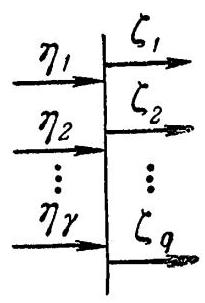
\includegraphics[max width=0.2\textwidth]{images/bo_d547imjef24c73bgfcdg_196_1213_1355_205_303_0.jpg}
\end{center}
\hspace*{3em}

Prac. 77.

Пусть теперь \({e}_{i}^{1},\ldots,{e}_{i}^{r}\) - координаты вершины \({e}_{i}\) многогранника U. Положим

\[
{u}^{\rho } = \frac{1}{2}\mathop{\sum }\limits_{{\alpha  = 1}}^{q}\left( {1 - {\chi }_{\alpha }}\right) {e}_{\alpha }^{\rho },\;\rho  = 1,\ldots ,r \tag{85}
\]

(рис. 79). Из (85) ясно, что точка ( \({u}^{1},\ldots,{u}^{r}\) ) совпадает с вершиной \({e}_{i}\), если \({\chi }_{i} =  - 1\), a остальные величины \({\chi }_{\alpha }\)

\begin{center}
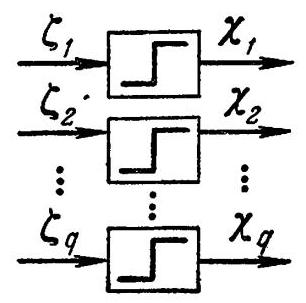
\includegraphics[max width=0.2\textwidth]{images/bo_d547imjef24c73bgfcdg_197_342_796_306_303_0.jpg}
\end{center}
\hspace*{3em}

Pnc. 78.

\begin{center}
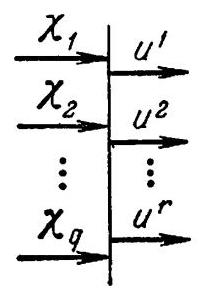
\includegraphics[max width=0.2\textwidth]{images/bo_d547imjef24c73bgfcdg_197_954_802_199_293_0.jpg}
\end{center}
\hspace*{3em}

Pnc. 79.

равны +1. Иначе говоря, если уравнение (81) имеет единственное решение, то этим решением является точка \(\left( {{u}^{1},\ldots,{u}^{r}}\right)\), получаемая по формулам (85).

Соединим теперь объекты, изображенные на рис. 67, 68, 75—79, вместе. Мы получим схему, показанную на рис. 80. Из сказанного выше ясно, что, каков бы ни был

\begin{center}
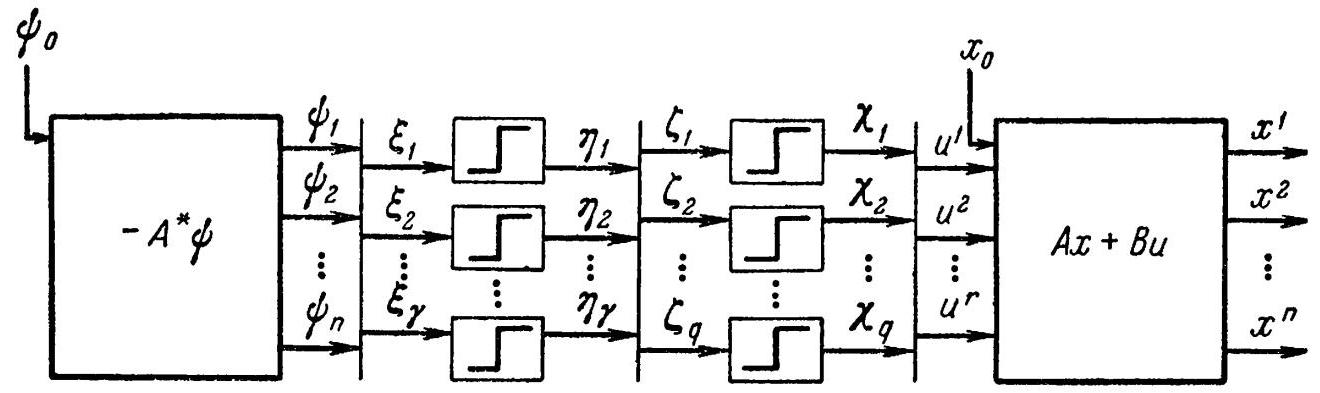
\includegraphics[max width=1.0\textwidth]{images/bo_d547imjef24c73bgfcdg_197_98_1528_1320_393_0.jpg}
\end{center}
\hspace*{3em}

Prac. 80.

начальный вектор \({\psi }_{0}\), \(\phi\) ункции \({u}^{1}\left( t\right),\ldots,{u}^{r}\left( t\right)\),получаю- щиеся на выходе предпоследнего звена, образуют экстремальное управление (ибо они удов. летворяют уравнению (6)), a на выходе схемы мы полу- чаем величины \({x}^{1}\left( t\right),\ldots,{x}^{n}\left( t\right)\), оитсhвающие соответ- ствующую экстремальную траекторию.

Итак, схема, изображенная на рис. 80, осуществля- ет движение объекта (2) по экстремальной траектории (при любых начальных значениях цо, хо).

Остается, как мы отмечали выше, задача поиска такого начального значения для ф, при котором (для заданного начального значения \({x}_{0}\) ) получаемая траектория проходит через начало координат. Такой поиск можно производить одним из следующих двух методов: либо, имея фиксиро- ванное начальное значение \({x}_{0}\),при помощи нескольких проб найти требуемое начальное значение фо, либо же, обратив направление течения времени, вычертить доста- точно густую сетку траекторий, исходящих из начала координат (они все будут оптимальными), после чего, «запомнив» все точки фазового пространства X, в кото- рых происходят переключения, составить «поверхность переключений» (т. е. произвести синтез оптимальных управлений).

Следует еще отметить возможность осуществить более быстрое течение времени в моделирующем устройстве по сравнению с реальным объектом (за счет подбора пара- метров в первом и последнем звеньях схемы). Это может позволить испробовать на моделирующем устройстве не- сколько экстремальных траекторий в течение короткого времени и получить требуемое оптимальное управление для исходного объекта.

\section*{§ 23. Линейные уравнения с переменными коэффициентами}

Основные факты, установленные в предыдущих пара- графах для линейных однородных уравнений с постоян- ными коэффициентами (см. (1)), переносятся и на случай линейных неоднородных уравнений с переменными коэф- фициентами. В этом параграфе мы приведем формули- ровки получаемых таким образом теорем и укажем те изменения, которые следует произвести в предыдущих доказательствах для получения этих теорем.

Уточним прежде всего п о с т а н о в к у з а д а ч и. Мы будем рассматривать объект, закон движения которого записывается в виде следующей линейной системы диффе- ренциальных уравнений:

\[
\frac{d{x}^{i}}{dt} = \mathop{\sum }\limits_{{v = 1}}^{n}{a}_{v}^{i}\left( t\right) {x}^{v} + \mathop{\sum }\limits_{{\rho  = 1}}^{r}{b}_{\rho }^{i}\left( t\right) {u}^{\rho } + {f}^{i}\left( t\right) ,\;i = 1,\ldots ,n. \tag{86}
\]

Областью управления \(U\) по-прежнему будем считать вы- пуклый замкнутый многогранник r-мерного пространства \({E}_{r}\) переменных \({u}^{1},\ldots,{u}^{r}\). Как и выше, ограничимся рас- смотрением задачи об оптимальных быстродействиях. Отно- сительно функций \({a}_{j}^{i}\left( t\right),{b}_{k}^{i}\left( t\right)\) и \({f}^{i}\left( t\right)\),входящих в систе- му (86), мы будем предполагать, что они определены на некотором интервале a < t < b (возможно, совпадающим со всей числовой прямой) и имеют на этом интервале достаточное число непрерывных производных. Именно, мы будем предполагать, что функции \({a}_{j}^{i}\left( t\right)\) имеют \(n - 2\) непрерывных производных (но не менее одной), функции \({b}_{k}^{i}\left( t\right)\) имеют \(n - 1\) непрерывную производную, а функ- ции \({f}^{i}\left( t\right)\) имеют одну непрерывную производную. (Воз- можность некоторого ослабления этих ограничений ука- зана в замечании, приведенном в конце этого параграфа.) Все рассматриваемые значения переменного \(t\) мы будем предполагать принадлежащими интервалу а < t < b; в частности, всякое допустимое управление будет предпо- лагаться заданным на отрезке, являющимся ча с т ь ю интервала а < t < b.

В векторной форме система (86) может быть записана следующим образом:

\[
\frac{dx}{dt} = A\left( t\right) x + B\left( t\right) u + f\left( t\right) ; \tag{87}
\]

здесь \(A\left( t\right)  : X \rightarrow  X\) и \(B\left( t\right)  : {E}_{r} \rightarrow  X\) — линейные операторы, определяемые в координатах \({x}^{1},\ldots,{x}^{n}\) и \({u}^{1},\ldots,{u}^{r}\) матрицами \(\left( {{a}_{j}^{i}\left( t\right) }\right)\) и б \(\left( {{b}_{k}^{i}\left( t\right) }\right)\) соогветственно, \(\mathrm{a}f\left( t\right)\) — вектор c компонентами \({f}^{i}\left( t\right)\).

Введем в рассмотрение операторы \({B}_{1}\left( t\right),{B}_{2}\left( t\right)\), \(\ldots,{B}_{n}\left( t\right),\pi\) оложив

\[
{B}_{1}\left( t\right)  = B\left( t\right) ,\;{B}_{j}\left( t\right)  =  - A\left( t\right) {B}_{j - 1}\left( t\right)  + \frac{d{B}_{j - 1}\left( t\right) }{dt}, \tag{88}
\]

\[
j = 2,\ldots ,n\text{ . }
\]

(Для возможности определения этих операторов необходи- мо, чтобы функции \({b}_{k}^{i}\left( t\right)\) имели л−1 производную, а функ- ции \({a}_{j}^{i}\left( t\right)\) имели л—2 производных.) Мы будем говорить, что в момент времени t выполнено условие общности положения, если для любого ребра w многогранника \(U\) векторы

\[
{B}_{1}\left( t\right) w,{B}_{2}\left( t\right) w,\ldots ,{B}_{n}\left( t\right) w \tag{89}
\]

линейно независимы в пространстве Х. В этом параграфе мы будем всюду предполагать, что в любой момент времени \(t,a < t < b\), выполнено условие общности положения.

Отметим, что если матрицы \(\left( {{a}_{j}^{i}\left( t\right) }\right)\) и ( \({b}_{k}^{i}\left( t\right)\) ) постоянны, т. е. величины \({a}_{j}^{i}\) и \({b}_{k}^{i}\) не зависят от времени, то из (88) следует,что \({B}_{j} = {\left( -1\right) }^{j - 1}{A}^{j - 1}B\),и потому векторы (89) совпадают, с точностью до знаков, с векторами (3). Таким образом, в этом случае сформулированное здесь условие общности положения совпадает с условием общности поло- жения, введенным в \$ 17.

Функция \(H\left( {\psi,x,t,u}\right)\) (см. стр. 73 и теорему 5) в рас- сматриваемом случае имеет вид

\[
H = \left( {\psi ,A\left( t\right) x}\right)  + \left( {\psi ,B\left( t\right) u}\right)  + \left( {\psi ,f\left( t\right) }\right)  =
\]

\[
= \mathop{\sum }\limits_{{\mu ,\nu }}{\psi }_{\mu }{a}_{\nu }^{\mu }\left( t\right) {x}^{\nu } + \mathop{\sum }\limits_{{\mu ,\rho }}{\psi }_{\mu }{b}_{\rho }^{\mu }\left( t\right) {u}^{\rho } + \mathop{\sum }\limits_{\mu }{\psi }_{\mu }{f}^{\mu }\left( t\right) , \tag{90}
\]

а вспомогательная система (см. формулу (69) гл. 1) записывается в виде

\[
\frac{d{\psi }_{j}}{dt} =  - \mathop{\sum }\limits_{v}{a}_{j}^{v}\left( t\right) {\psi }_{v},\;j = 1,2,\ldots ,n,
\]

или,в векторной форме (ср. 5)),

\[
\frac{d\psi }{dt} =  - {A}^{ * }\left( t\right) \psi . \tag{91}
\]

Очевидно, что функция \(H\), рассматриваемая как функция переменного исси, достигает максимума одно- временно с функцией (ф, в(t)u). Максимум функции \(\left( {\psi,B\left( t\right) u}\right)\), рассматриваемой как функция переменного \(u \in  U\),мы обозначим через \(P\left( {\psi,t}\right)\). Из теоремы 5 следует (см. формулу (70) гл. 1), что если и(t), бо ≤ t ≤ t, — опти- мальное управление, переводящее фазовую точку из положения \({x}_{0}\) в положение \({x}_{1}\), то существует такое нетривиальное репение \(\psi \left( t\right)\) уравнения (91), что

\[
\left( {\psi \left( t\right) ,B\left( t\right) u\left( t\right) }\right)  = P\left( {\psi \left( t\right) ,t}\right) \tag{92}
\]

для всех t, принадлежащих отрезку \({t}_{0} \leq  t \leq  {t}_{1}\).

Некоторую функцию, заданную на интервале а < t < b или на его части, мы будем называть кусочно-постоянной, если множество всех точек разрыва этой функции не имеет предельных точек внутри интервала а на каждом из интервалов, на которые интервал \(a < t < b\) разбивается этими точками разрыва, рассматриваемая функция постоянна. (Заметим, что точки разрыва могут накапливаться к концам интервала а < t < b.)

Т е о р е м а 15. Для каждого нетривиального решения \(\psi \left( t\right)\) уравнения (91) соотношение (92) однозначно *) опре- деляет управляющую функцию и(t); при этом оказывает- ся, что функция и(t) кусочно-постоянна и ее значениями являются лишь вершины многогранника U.

Это — теорема о «конечности числа переключений» для линейных уравнений с переменными коэффициентами (ибо всякое управление \(u\left( t\right)\) задано на некотором о т р е з к е \({t}_{0} \leq  t \leq  {t}_{1}\),целиком лежащем внутри интервала а < t < b, и из теоремы 15 следует, что число точек разрыва функ- ции \(u\left( t\right)\) конечно). В случае постоянных коэффициентов теорема 15 превращается в теорему 9.

До ка за те л ь с т в о теоремы 15 вполне аналогично доказательству теоремы 9. Укажем лишь те незначитель- ные изменения, которые следует произвести в доказатель- стве теоремы 9.

Предположим, что множество точек, в которых зна- чение управления и(t) не определяется однозначно соот- ношением (92), имеет хотя бы одну предельную точку в н у т р и интервала а < t < b. Тогда, как и выше (см. формулу (8) и относящийся к ней текст), мы сможем найти такое ребро м многогранника U и такое множество \(M\), имеющее внутри интервала а < t < b пре- дельную точку т, что

\[
\left( {\psi \left( t\right) ,B\left( t\right) w}\right)  = 0 \tag{93}
\]

при всех t ∈ M.

\HRule

*) Cp. сноску на стр. 130.

\HRule

Формула (9) заменяется соотношением

\[
\left( {\psi \left( t\right) ,B\left( t\right) w}\right)  = \mathop{\sum }\limits_{{v,\rho }}{\psi }_{v}\left( t\right) {b}_{\rho }^{v}\left( t\right) {w}^{\rho }. \tag{94}
\]

Так как функции \({a}_{j}^{i}\left( t\right)\) имеют л—2 непрерывных произ- водных, то функции \({\psi }_{1}\left( t\right),\ldots,{\psi }_{n}\left( t\right)\), составляющие ре- шение уравнения (91), имеют л–1 непрерывную произ- водную; функции \({b}_{\rho }^{v}\left( t\right)\) также имеют, по предположению, \(n - 1\) непрерывную производную. Следовательно, функция (94) n-1 раз непрерывно дифференцируема.

Так как τ — предельная точка множества М, то, в силу непрерывности функции (94), из соотношения (93) выте- кает, что

\[
\left( {\psi \left( \tau \right) ,B\left( \tau \right) w}\right)  = 0.
\]

Далее, так как между каждыми двумя корнями дифферен- цируемой функции содержится хотя бы один корень ее производной, то производная функции (94) обращается в нуль в бесконечном множестве точек, имеющем т своей предельной точкой. Но производная функции (94) имеет вид

\[
\frac{d}{dt}\left( {\psi \left( t\right) ,B\left( t\right) w}\right)  = \left( {-{A}^{ * }\left( t\right) \psi \left( t\right) ,B\left( t\right) w}\right)  + \left( {\psi \left( t\right) ,\frac{{dB}\left( t\right) }{dt}w}\right)  =
\]

\[
= \left( {\psi \left( t\right) , - A\left( t\right) B\left( t\right) w}\right)  + \left( {\psi \left( t\right) ,\frac{{dB}\left( t\right) }{dt}w}\right)  = \left( {\psi \left( t\right) , - {B}_{2}\left( t\right) w}\right)
\]

(см. (88)). Таким образом, на бесконечном множестве то- чек, имеющем т своей предельной точкой, выполняется соотношение

\[
\left( {\psi \left( t\right) ,{B}_{2}\left( t\right) w}\right)  = 0,
\]

и потому (в силу непрерывности)

\[
\left( {\psi \left( \tau \right) ,{B}_{2}\left( \tau \right) w}\right)  = 0.
\]

Аналогично, между любыми двумя корнями функции \(\left( {\psi \left( t\right),{B}_{2}\left( t\right) w}\right)\) содержится хотя бы один корень ее про- изводной; из этого с помощью тех же рассуждений по- лучаем (ψ(τ), \({B}_{3}\left( \tau \right) w) = 0\) и т. д. В результате мы получаем соотношения

\[
\left( {\psi \left( \tau \right) ,{B}_{i}\left( \tau \right) w}\right)  = 0,\;i = 1,2,\ldots ,n \tag{95}
\]

(cp. (10), (11)). В силу линейной независимости векторов (89) из соотношений (95) вытекает, что ψ(τ) = 0, и потому решение ψ(t) уравнения (91) тривиально. Полученное противоречие показывает, что множество точек, в кото- рых управление и(t) не определяется однозначно соотно- шением (92), не имеет предельных точек внутри интер- вала \(a < t < b\).

Дальнейшее доказательство не отличается от доказа- тельства теоремы 9. Итак, теорема 15 доказана.

Перейдем теперь к рассмотрению т е о р е м с у щ е - ство в ания и единственности для системы (86). Как и выше (см. (20)), рассмотрим фундаменталь- ную систему решений

\[
{\varphi }_{1}\left( t\right) ,\ldots ,{\varphi }_{n}\left( t\right)
\]

однородного уравнения \(\frac{dx}{dt} = A\left( t\right) x\), удовлетворяющую на- чальным условиям Фубко) = б, и фундаментальную сис- тему решений

\[
{\psi }^{1}\left( t\right) ,\ldots ,{\psi }^{n}\left( t\right)
\]

уравнения (91), удовлетворяющую начальным условиям \({\psi }_{i}^{j}\left( {t}_{0}\right)  = {\delta }_{i}^{j}\). При этом соотношение (21) остается справед- ливым. Далее, решение уравнения (87), соответствующее произвольно выбранному управлению и(t), \({t}_{0} \leq  t \leq  {t}_{1}\), можно искать в виде

\[
x\left( t\right)  = \mathop{\sum }\limits_{{v = 1}}^{n}{\varphi }_{v}\left( t\right) {c}^{v}\left( t\right)
\]

(cp. стр. 138). В результате мы получаем следующую формулу (ср. (22)):

\[
x\left( t\right)  = \mathop{\sum }\limits_{{v = 1}}^{n}{\varphi }_{v}\left( t\right) \left( {{x}_{0}^{v} + {\int }_{{t}_{0}}^{t}\left( {{\psi }^{v}\left( t\right) ,B\left( t\right) u\left( t\right)  + f\left( t\right) }\right) {dt}}\right) . \tag{96}
\]

После этого теоремы 11 и 12 (в дословно тех же форму- лировках) переносятся и на рассматриваемый случай. Сохраняются и доказательства этих теорем — с заменой соотношения (22) соотношением (96) и вытекающими от- сюда очевидными изменениями. Сохраняется и теорема существования (см. теорему 13).

Т е о р е м а 16. Если для процесса, описываемого уравне- нием (87), существует при заданном \({t}_{0}\) хотя бы одно управ- ление \(u\left( t\right),{t}_{0} \leq  t \leq  {t}_{1}\), переводящее фазовую точку из поло- жения \({x}_{0}\) в положение \({x}_{1}\), то существует и оптимальное управление (с тем же начальным моментом \({t}_{0}\)), переводящее фазовую точку из положения \({x}_{0}\) в положение \({x}_{1}\).

До к а з а т е л ь с т в о является дословным повторе- нием доказательства теоремы 13 (с очевидной заменой ссы- лок на формулу (22) ссылками на формулу (96)). Отметим только, что сдвиг времени, о котором упоминалось на стр. 143, теперь не может быть применен ввиду того, что уравнение (87) неавтономно; однако этот сдвиг вре- мени теперь и не нужен, так как рассматриваются лишь управления с начальным моментом \({t}_{0}\).

Замечание. Все результаты настоящего параграфа получены в предположении, что функции \({a}_{j}^{i}\left( t\right),{b}_{k}^{i}\left( t\right)\) и \({f}^{i}\left( t\right)\), входящие в систему (86), определены на некотором интервале \(a < t < b\) (возможно,на всей прямой) и функ- ции \({f}^{i}\left( t\right)\) имеют на этом интервале первые непрерывные производные, а функции \({a}_{j}^{i}\left( t\right)\) и \({b}_{k}^{i}\left( t\right)\) имеют соответствен- ные \(\left( {n - 2}\right)\) -e и (n-1)-e непрерывные производные. (Кро- ме того, как всегда, предполагалось выполненным усло- вие общности положения.) Нетрудно понять, что все полученные результаты остаются справедливыми, если функции \({a}_{j}^{i}\left( t\right),{b}_{k}^{i}\left( t\right),{f}^{i}\left( t\right)\) непрерывны, а их производные (в указанном числе) являются лишь к у с о ч н о - н е п р е- р ы в н ы м и функциями. В самом деле, отметим на интервале а < t < b все точки, в которых хотя бы одна из указанных производных терпит разрыв непрерывности. Эти точки разбивают интервал \(a < t < b\) на части, на каждой из которых функции \({a}_{j}^{i}\left( t\right),{b}_{k}^{i}\left( t\right),{f}^{i}\left( t\right)\) имеют тре- буемое число непрерывных производных. К каждой из этих частей в отдельности можно применить теорему 15, и потому теорема 15 справедлива в применении ко всему интервалу \(a < t < b\). Очевидно, что остается справедли- вой и формула (96), а потому также и теоремы сущест- вования и единственности.

\section*{РАЗНЫЕ ЗАДАЧИ}

\section*{§ 24. Случай функционала, заданного несобственным интегралом}

Рассмотрим следующий вариант оптимальной задачи, сводящийся к рассмотрению бесконечного интервала ин- тегрирования в функционале J.

В фазовом пространстве X дана точка \({x}_{0}\). Среди всех допустимых управлений \(u\left( t\right)\), \({t}_{0} \leq  t < \infty\), для которых соответствующая траектория \(x\left( t\right)\) системы

\[
\frac{d{x}^{i}}{dt} = {f}^{i}\left( {{x}^{1},\ldots ,{x}^{n},u}\right) ,\;i = 1,\ldots ,n,u \in  U, \tag{1}
\]

исходящая из точки \({x}_{0}\), определена для всех \({t}_{0} \leq  t\) и удов- летворяет при \(t \rightarrow \infty\) некоторым (заданным заранее) предельным условиям, найти такое, для которого интеграл

\[
J = {\int }_{{t}_{0}}^{\infty }{f}^{0}\left( {x\left( t\right) ,u\left( t\right) }\right) {dt} \tag{2}
\]

сходится и принимает наименьшее возможное значение.

На функции \({f}^{i}\left( {x,u}\right)\) накладываются условия, аналогич- ные тем, которые были указаны в гл. 1,2: они пред- полагаются непрерывными по х и и и непрерывно диффе- ренцируемыми по \({x}^{1},\ldots,{x}^{n}\) на прямом произведении \(X \times  \overline{U}\). Отметим далее, что мы будем понимать здесь под «допустимыми» управлениями. Функцию \(u\left( t\right),{t}_{0} \leq  t < \infty\), принимающую значения в области управления U, мы будем считать о г р а н и ч е н н о й, если множество всех точек \(u\left( t\right)\), где t пробегает любой к о н е ч н ы й отрезок, лежащий на промежутке \({t}_{0} \leq  t < \infty\), имеет в простран- стве E, (содержащем область управления U) компактное замыкание. Принимая это определение ограниченности управления (и рассматривая лишь управления, заданные на промежутках вида \({t}_{0} \leq  t < \infty\) ), мы в остальном сохра- ним определение класса допустимых управлений, данное в \$ 10. В частности, в качестве класса допустимых управ- лений можно взять класс всех ограниченных (в указан- ном смысле) измеримых управлений, заданных на промежутках вида \({t}_{0} \leq  t < \infty\),или же класс всех огра- ниченных кусочно-непрерывных управлений (кусочная непрерывность понимается в том смысле, что на всяком к о н е ч н о м отрезке, содержащемся в промежутке бо ≤ \(\leq  t < \infty\), управление и(t) имеет лишь конечное число разрывов первого рода). Наконец, сделаем еще замеча- ния относительно «предельных условий на бесконечнос- ти», упомянутых в формулировке задачи. Мы предпола- гаем, что эти условия имеют вид

\[
\mathop{\lim }\limits_{{t \rightarrow  \infty }}{x}^{i}\left( t\right)  = {x}_{1}^{i} \tag{3}
\]

где \({x}_{1} = \left( {{x}_{1}^{1},{x}_{1}^{2},\ldots,{x}_{1}^{n}}\right)  - 3\) аданная точка фазового про- странства \(X\). Если для фазовой траектории \(x\left( t\right)\), соответ- ствующей допустимому управлению \(u\left( t\right)\) и исходящей из точки \({x}_{0}\), выполнены условия (3), то мы будем писать \(x\left( \infty \right)  = {x}_{1}\) и будем говорить, что управление \(u\left( t\right)\), \({t}_{0} \leq \; \leq  t < \infty\), переводит фазовую точку из положения хо в по- ложение \({x}_{1}\).

Решение поставленной оптимальной задачи дается тео- ремой 1 (или теоремой 8) с очевидной заменой отрезка \({t}_{0} \leq  t \leq  {t}_{1}\) бесконечным промежутком \({t}_{0} \leq  t < \infty\) и с за- меной условия прохождения траектории через некоторую точку прямой П предельными условиями на бесконечнос- ти. В самом деле, все рассуждения, приведенные в \$8 13, 14, были связаны с выбором некоторой правильной точ- ки т, удовлетворяющей условию т < t, эти рассуждения дословно, без всяких изменений проходят и в случае \({t}_{1} = \infty\). To же относится к формулировке и доказатель ству лемм 5—8 из § 15. Однако построение предельного конуса уже не проходит, так как точки и (правого кон- ца отрезка времени) не существует. Тем не менее, легко видоизменить конструкцию предельного конуса таким образом, чтобы ее можно было применить и в рассматри- ваемом случае. В самом деле, обозначим через \({K}_{{t}_{0}}^{\left( \tau \right) }\) вы- пуклый конус Ат,-1(Кт). Эти конусы образуют возрастаю- щую последовательность: \({K}_{{t}_{0}}^{\left( {\tau }^{\prime }\right) } \subset  {K}_{{t}_{0}}^{\left( \tau \right) }\) при \({\tau }^{\prime } < \tau\) (для до- казательства этого факта достаточно к включению, содержащемуся в лемме 8, применить преобразование \({A}_{\tau,{t}_{0}}^{-1}\) и воспользоваться формулами (17) гл. 2). Поэтому объеди- нение (по всем правильным точкам т) всех конусов К (т снова есть выпуклый конус (возможно, не замкнутый) пространства \({X}_{{t}_{0}}\). Назовем его на чал ь н ы м к о н у - у с о м и обозначим через ку. Легко видеть, что (для рас- сматривавшейся в \$§ 2, 11 оптимальной задачи) имеет место соотношение

\[
{A}_{{t}_{1},{t}_{0}}\left( {\mathbf{K}}_{{t}_{0}}\right)  = {\mathbf{K}}_{{t}_{1}}.
\]

Поэтому начальный конус совершенно эквивалентен пре- дельному, и можно было завершение доказательства прин- ципа максимума (§ 15, после леммы 8) провести с помо- щью н а ч а л ь н о г о к о н у с а Ки,- При этом лемма 9, как и ее доказательство, остается в силе (с очевидной заменой луча \({L}_{{t}_{1}}\),конусов \({K}_{{t}_{1}},{K}_{{t}_{1}}^{\left( \tau \right) }\) и преобразований \({A}_{{t}_{1},\tau }^{-1}\) соогветственно на \({L}_{{t}_{0}},{K}_{{t}_{0}},{K}_{{t}_{0}},{K}_{{t}_{0}}^{\left( \tau \right) }\) и \({A}_{\tau,{t}_{0}}\) ). После этого без труда проводятся и заключительные рассужде- ния § 15, чем доказательство теоремы 8 (и теоремы 1), проводимое с помощью на ча л ь н о г о конуса (вместо предельного) и завершается. Но такое доказательство до- словно (с заменой отрезка to ≤ t ≤ t, промежутком бо ≤ \(\leq  t < \infty\) ) переносится и на случай рассматриваемой опти- мальной задачи (1), (2). Тем самым наше утверждение доказано.

Заметим еще, что можно было «сносить» конусы к не в точку х или в точку хе(би), а в любую точку \(x\left( t\right)\) рассматриваемой траектории. Поэтому изложенное доказательство применимо и к случаю, когда промежут- ком интегрирования является вся прямая — \(\infty  < t < \infty\).

\section*{§ 25. Оптимальные процессы с параметрами}

Мы рассмотрим в этом параграфе следующую опти- мальную задачу. Функции \({f}^{0},{f}^{1},\ldots,{f}^{n}\) зависят от трех переменных \(x \in  X,u \in  U,w \in  W\),где \(X\) и \(U\) имеют преж- ний смысл, а W — векторное пространство размерности m. Функции \({f}^{0},{f}^{1},\ldots,{f}^{n}\) и их частные производные по всем переменным \({x}^{1},{x}^{2},\ldots,{x}^{n}\) предполагаются определен- ными и непрерывными на всем пространстве \(X \times  \overline{U} \times  W\). Закон движения объекта задается уравнениями

\[
\frac{d{x}^{i}}{dt} = {f}^{i}\left( {x,u,w}\right) ,\;i = 1,2,\ldots ,n. \tag{4}
\]

В пространстве X заданы две точки х, и требуется выбрать такую п о с т о я н н у ю точку му не не не не не не не не начала движения подобрать значение параметра w, оста- ющееся постоянным в течение всего движения) и такое допустимое управление и(t), чтобы соответствующая траектория \(x\left( t\right)\), исходящая в момент и из точки х,, проходила в некоторый момент \({t}_{1}\) через точку и чтобы при этом интеграл

\[
J = {\int }_{{t}_{0}}^{{t}_{1}}{f}^{0}\left( {x\left( t\right) ,u\left( t\right) ,{w}_{0}}\right) {dt}
\]

принимал наименьшее возможное значение. Если функ- ции \(u\left( t\right),x\left( t\right)\) и точка мо дают решение поставленной задачи, то величины и(t), х(t), му мы будем называть оптимальными (для заданных точек к и и и и).

При решении этой задачи мы будем предполагать, что все допустимые функции к у с о ч н о - н е п р е р ы в- н ы, т. е. что класс D допустимых управлений либо сов- падает с множеством всех кусочно-непрерывных функций (со значениями в U), либо является его подмножеством, удовлетворяющим условиям, указанным в \$ 10.

Отметим некоторую специфику рассматриваемой зада- чи, заставляющую ограничиваться лишь кусочно-непре- рывными (а не произвольными измеримыми) управления- ми. В то время как в оптимальной задаче, сформулиро- ванной в \$ 11, каждый кусок оптимальной траектории снова является оптимальной траекторией (ибо «улучше- ние» куска траектории ведет к «улучшению» всей траек- тории, ср. § 2), здесь, в рассматриваемой задаче с пара- метрами это уже не так. Ведь оптимальные значения параметра и для всей траектории и для ее части могут не совпадать, т. е. если и(t), \({w}_{0}\) дают решение поставлен- ной в этом параграфе оптимальной задачи, причем управле- ние \(u\left( t\right)\) определено на отрезке \({t}_{0} \leq  t \leq  {t}_{1}\), to на меньшем отрезке за с чет и зменения параметра ию возможно удастся «улучшить» управление и(t). Из ска- занного следует, что рассуждения, проведенные при до- казательстве леммы 4, н е п р и м е н и м ы к рассматривае- мой оптимальной задаче. Рассуждения, доказывающие теорему 8 (или теорему 1), можно, однако, применить и здесь, считая в лемме 9 точку т совпадающей с к о н - цевой точкой и (что делает излишней лемму 4). Но для этого приходится считать точку и п р а в и л ь н о й т о ч к о й управления \(u\left( t\right)\), т. е. в качестве допустимых управлений приходится брать управления, правильные в правом конце отрезка. При этих условиях наиболее естественным классом допустимых управлений является класс кусочно-непрерывных управлений (или какой-либо его подкласс).

Решение поставленной оптимальной задачи дается сле- дующей теоремой, аналогичной теореме 1 (функция Ж определяется, как и прежде: Ж \(= \mathop{\sum }\limits_{{\alpha  = 0}}^{n}{\psi }_{\alpha }{f}^{\alpha }\) ).

T e o p e m a 17. Пусть и(t), t’est e t, - такое допус- тимое управление, а шу те тет не значнем на не значение параметра w, что соответствующая траектория

\[
x\left( t\right)  = \left( {{x}^{0}\left( t\right) ,{x}^{1}\left( t\right) ,\ldots ,{x}^{n}\left( t\right) }\right)  = \left( {{x}^{0}\left( t\right) ,x\left( t\right) }\right)
\]

(т. е. траектория системы (4), пополненной соот- ветствующим уравнением для i = 0) удовлетворяет усло- виям \(x\left( {t}_{0}\right)  = {x}_{0},{x}^{0}\left( {t}_{0}\right)  = 0,x\left( {t}_{1}\right)  = {x}_{1}\). Для того чтобы величины \(u\left( t\right),\;x\left( t\right),\;{w}_{0}\) давали решение поставлен- ной оптимальной задачи, необходимо существование такой ненулевой непрерывной вектор-функции Ф(н) \(= \left( {{\psi }_{0}\left( t\right),{\psi }_{1}\left( t\right),\ldots,{\psi }_{n}\left( t\right) }\right),{umo} :\)

1 \textdegree  функции \(x\left( t\right),\psi \left( t\right),u\left( t\right)\) и значение шо удовлетворяют гамильтоновой системе

\[
\left. \begin{array}{l} \frac{d{x}^{i}}{dt} = \frac{\partial \mathcal{K}\left( {\psi \left( t\right) ,x\left( t\right) ,u\left( t\right) ,{w}_{0}}\right) }{\partial {\psi }_{i}}, \\  \frac{d{\psi }_{i}}{dt} =  - \frac{\partial \mathcal{K}\left( {\psi \left( t\right) ,x\left( t\right) ,u\left( t\right) ,{w}_{0}}\right) }{\partial {x}^{i}}, \end{array}\right\}  i = 0,1,\ldots ,n;
\]

\(2{}^{ \circ  }\) функция \(\mathcal{K}\left( {\psi \left( t\right) ,x\left( t\right) ,u,{w}_{0}}\right)\) переменного \(u \in  U\) достигает в точке и = и(t) максимума

\[
\mathcal{K}\left( {\psi \left( t\right) ,x\left( t\right) ,u\left( t\right) ,{w}_{0}}\right)  = \mathcal{M}\left( {\psi \left( t\right) ,x\left( t\right) ,{w}_{0}}\right) ; * )
\]

\({3}^{ \circ  }\;\text{ е }\;\texttt{ hauanbhout mouke }{t}_{0}\;{\text{ в }\text{ ы }\text{ п }\text{ о }\text{ л }\text{ н }\text{ е }\text{ н }\text{ ы }}\;{\text{ с }\text{ о }\text{ о }\text{ т }\text{ н }\text{ о }\text{ ш }\text{ е }\text{ н }\text{ ц }\text{ я }}\)

\[
{\psi }_{0}\left( {t}_{0}\right)  \leq  0,\mathcal{M}\left( {\psi \left( {t}_{0}\right) ,x\left( {t}_{0}\right) ,{w}_{0}}\right)  = 0;
\]

\({4}^{ \circ  }\) u.merom mecmo paseнсmea

\[
\mathop{\sum }\limits_{{\alpha  = 0}}^{n}{\int }_{{t}_{0}}^{{t}_{1}}{\psi }_{\alpha }\left( t\right) \frac{\partial {f\alpha }\left( {x\left( t\right) ,u\left( t\right) ,{w}_{0}}\right) }{\partial {w\rho }}{dt} = 0,\rho  = 1,\ldots ,m. \tag{5}
\]

Оказывается, далее, что если величины ψ(t), x(t), w, \(u\left( t\right) y\partial o\) влетворяют условиям 1 \textdegree  и 2 \textdegree, то функции у фо \(u \sim  \mathcal{M}\left( {\psi \left( t\right),x\left( t\right),{w}_{0}}\right)\) переменного \(t\) являются постоянны- ми, так что проверку условия 3 \textdegree  можно проводить не обязательно в момент \({t}_{0}\), a в любой момент \(t\), \({t}_{0} \leq  t \leq  {t}_{1}\).

Эта теорема отличается от теоремы 1 (или теоремы 8) наличием условия 4 \textdegree, которое дает m дополнительных соотношений, что и дает возможность решать задачу, так как в эту задачу введено дополнительно m неиз- вестных \({w}^{1},{w}^{2},\ldots,{w}^{m}\) (координаты точки \({w}_{0}\) в про- странстве \(W\) ).

Укажем, какие изменения нужно произвести в дока- зательстве теоремы 8, чтобы получить доказательство теоремы 17. Конструкции § 12 несколько видоизменяются.

Именно, пусть и (t) — произвольное допустимое управ- ление, заданное при \({t}_{0} \leq  t \leq  {t}_{1}\) ; далее, \(w -\) некоторое значение параметра, \(\mathrm{a}x\left( t\right)  = \left( {{x}^{0}\left( t\right),{x}^{1}\left( t\right),\ldots,{x}^{n}\left( t\right) }\right)  = \; = \left( {{x}^{0}\left( t\right),x\left( t\right) }\right)\) — соответствующее управлению и (1) и пара- метру w решение системы (4) с начальным условием \(x\left( {t}_{0}\right)  = {x}_{0}\). Обозначим через у (t) решение, соответствую- щее тому же управлению и (t) и значению параметра \(w + {\varepsilon \delta w}\) и исходящее (в тот же момент \({t}_{0}\) ) из близкой \(\mathbf{K}{x}_{0}\) TO4KU \({y}_{0} = {x}_{0} + \varepsilon {\xi }_{0} + o\left( \varepsilon \right)\), RQE \({\xi }_{0}\) - постоянный (т. е. не зависящий от ε) вектор пространства Х. Ре- шение \(y\left( t\right)\) имеет вид

\[
y\left( t\right)  = x\left( t\right)  + {\varepsilon \delta x}\left( t\right)  + o\left( \varepsilon \right) ,
\]

\HRule

*) См. стр. 24.

\HRule

где \({\delta x}\left( t\right)  = \left( {\delta {x}^{0}\left( t\right),\delta {x}^{1}\left( t\right),\ldots,\delta {x}^{n}\left( t\right) }\right)  -\) не зависящий от ε вектор, определяемый следующей системой уравнений в вариациях:

\[
\frac{d}{dt}\delta {x}^{i} = \mathop{\sum }\limits_{{\alpha  = 0}}^{n}\frac{\partial f\left( {x\left( t\right) ,u\left( t\right) ,w}\right) }{\partial {x}^{\alpha }}\delta {x}^{\alpha } + \mathop{\sum }\limits_{{\beta  = 1}}^{m}\frac{\partial f\left( {x\left( t\right) ,u\left( t\right) ,w}\right) }{\partial {w}^{\beta }}\delta {w}^{\beta }, \tag{6}
\]

\[
i = 0,1,\ldots ,n,
\]

при начальном условии δx(t,0) = ξ0. В отличие от системы (16) в § 12, эта система уравнений в вариациях неод- нородна.

Преобразование \({A}_{t,{t}_{0}}\) мы теперь снабдим верхним индек- сом δw. Именно, мы будем полагать

\[
{A}_{t,{t}_{0}}^{\delta w}\left( {\xi }_{0}\right)  = {\delta x}\left( t\right)
\]

где \({\delta x}\left( t\right)\) — решение системы (6) при начальном условии \({\delta x}\left( {t}_{0}\right)  = {\xi }_{0}\). Как и в § 12, вектор \({A}_{t,{t}_{0}}^{\delta w}\left( {\xi }_{0}\right)\) мы будем счи- тать вектором пространства X, (с началом координат в точке х (t)). Поскольку система уравнений в вариа- циях теперь неоднородна, то линейное преобразование \({A}_{t,{t}_{0}}^{\delta w}\left( {\xi }_{0}\right)\) также будет неоднородным.

Наконец, лемма 1, завершающая § 12, примет следу- ющий вид:

если ψ (t) — решение системы (8) § 11, а ξ\_η произволь- ный вектор, заданный в точке \(x\left( {t}_{0}\right),{mo}\) на всем отрезке \({t}_{0} \leq  t \leq  {t}_{1}\) выполнено соотношение

\(\left( {\psi \left( t\right) ,{A}_{t,{t}_{0}}^{\delta w}\left( {\xi }_{0}\right) }\right)  = \left( {\psi \left( {t}_{0}\right) ,{\xi }_{0}}\right)  +\)

\[
+ {\int }_{{t}_{0}}^{t}\mathop{\sum }\limits_{{i = 0}}^{n}\mathop{\sum }\limits_{{\beta  = 1}}^{m}{\psi }_{i}\left( t\right) \frac{\partial {f}^{i}\left( {x\left( t\right) ,u\left( t\right) ,w}\right) }{\partial {w}^{\beta }}\delta {w}^{\beta }{dt}. \tag{7}
\]

Обратимся, далее, к § 13. Правильными точками управления \(u\left( t\right)\) являются все его точки непрерывности, т. e. все точки отрезка \({t}_{0} \leq  t \leq  {t}_{1}\),3a исключением конечного числа точек разрыва. Мы продолжим управле- ние \(u\left( t\right)\) несколько дальше, за правый конец отрезка \({t}_{0} \leq  t \leq  {t}_{1}\), полагая \(u\left( t\right)  = u\left( {{t}_{1} - 0}\right)\) nput \(t > {t}_{1}\). Продолжен- ное таким образом управление \(u\left( t\right)\) непрерывно в точке \({t}_{1}\), так что \({t}_{1}\) является правильной точкой. Далее, точку т, входящую в определение проварьированного управления (crp. 97), мы теперь будем считать совпадающей с би, т. е. положим

\[
{t}_{0} < {\tau }_{1} \leq  {\tau }_{2} \leq  \ldots  \leq  {\tau }_{s} \leq  \tau  = {t}_{1}.
\]

Наконец, мы выберем некоторый вектор δw простран- ства W и через x* (t) будем обозначать (при достаточно малом ε) решение системы

\[
\frac{d{x}^{i}}{dt} = {f}^{i}\left( {x,{u}^{ * }\left( t\right) ,{w}_{0} + {\varepsilon \delta w}}\right) ,\;i = 0,1,\ldots ,n,
\]

т. e. траекторию, соответствующую проварьированному управлению \({u}^{ * }\left( t\right)\) и смещенному значению \(w = {w}_{0} + {\varepsilon \delta w}\) параметра w. При этом линию ξ(ε) мы будем считать вы- родившейся в точку х, т. е. будем считать, что решение \({x}^{ * }\left( t\right)\) удовлетворяет тому же начальному условию

\[
{x}^{ * }\left( {t}_{0}\right)  = {x}_{0},
\]

что и решение \(x\left( t\right)\). Формулы (21),(22) гл. 2 теперь можно будет записать в виде

\[
{x}^{ * }\left( {{t}_{1} + {\varepsilon \delta t}}\right)  = x\left( {t}_{1}\right)  + {\varepsilon \Delta x} + o\left( \varepsilon \right) ,
\]

где

\[
{\Delta x} = f\left( {x\left( {t}_{1}\right) ,u\left( {t}_{1}\right) ,{w}_{0}}\right) {\delta t} + {A}_{{t}_{1},{t}_{0}}^{\delta w}\left( 0\right)  +
\]

\[
+ \mathop{\sum }\limits_{{i = 1}}^{s}{A}_{{t}_{1},{\tau }_{i}}^{\delta w}\left\lbrack  {f\left( {x\left( {\tau }_{i}\right) ,{v}_{i},{w}_{0}}\right)  - f\left( {x\left( {\tau }_{i}\right) ,u\left( {\tau }_{i}\right) ,{w}_{0}}\right) }\right\rbrack  \delta {t}_{i} \tag{8}
\]

(ибо ξ0=0).

Обратимся теперь к § 14. Мы включим вектор \({\delta w}\) в символ а, т. е. будем полагать

\[
a = \left\{  {{\tau }_{i},{v}_{i},\delta {t}_{i},{\delta t},{\delta w}}\right\}
\]

(мы опустили обозначение точки т, так как теперь т = н, есть фиксированная точка). Линейная комбинация сим- волов а определяется так же, как и раньше, только с учетом и последнего аргумента:

\[
{\lambda }^{\prime }\left\{  {\ldots ,\;\delta {w}^{\prime }}\right\}   + {\lambda }^{\prime \prime }\left\{  {\ldots ,\;\delta {w}^{\prime \prime }}\right\}   + \ldots  = \left\{  {\ldots ,\;{\lambda }^{\prime }\delta {w}^{\prime } + {\lambda }^{\prime \prime }\delta {w}^{\prime \prime } + \ldots }\right\}  .
\]

После этого доказательство лемм 2,3 (при т е ты про- ходит без изменения, а лемма 4 становится просто ненуж- ной (ибо τ = +1). В результате мы получаем конус дости- жимости \({K}_{{t}_{1}}\),для которого справедлива лемма 3.

Рассуждения § 15 также сохраняются (с заменой т на \({t}_{1}\) ), a предельный конус становится ненужным,так как у нас имеется лишь один конус Ки, построенный как раз в конце x(t, траектории x(t) (в силу этого лемма 9 не нужна — она просто сводится к лемме 3). Наконец, рассуждения, приведенные в конце \$ 15, доказывают (при δw = 0) условия 1 \textdegree, 2 \textdegree, 3 \textdegree  и заключительную часть теоремы 17.

Остается показать, что для выбранного таким образом вектора ф(н) выполняется условие 4 \textdegree. Положим в фор- муле (8) \({\delta t} = \delta {t}_{1} = \delta {t}_{2} = \ldots  = \delta {t}_{s} = 0\). Мы получим тогда

\[
{\Delta x} = {A}_{{t}_{1},{t}_{0}}^{\delta w}\left( 0\right) .
\]

Согласно сказанному выше (ср. формулы (34), (36) гл. 2), мы имеем (ψ( \({t}_{1}\) ), \({\Delta x}) \leq  0\) для любого вектора Δx вида (8), и потому (см. (7))

\[
\left( {\psi \left( {t}_{1}\right) ,{A}_{{t}_{1},{t}_{0}}^{\delta w}\left( 0\right) }\right)  = {\int }_{{t}_{0}}^{{t}_{1}}\mathop{\sum }\limits_{{i = 0}}^{n}\mathop{\sum }\limits_{{\beta  = 1}}^{m}{\psi }_{i}\left( t\right) \frac{\partial {f}^{i}\left( {x\left( t\right) ,u\left( t\right) ,{w}_{0}}\right) }{\partial {w}^{\beta }}\delta {w}^{\beta }{dt} \leq  0.
\]
 (7*)

Так как эти соотношения справедливы при любых дей- ствительных значениях параметров δwβ, то мы имеем

\[
\mathop{\sum }\limits_{{\alpha  = 0}}^{n}{\int }_{{t}_{0}}^{{t}_{1}}{\psi }_{\alpha }\left( t\right) \frac{\partial {f}^{\alpha }\left( {x\left( t\right) ,u\left( t\right) ,{w}_{0}}\right) }{\partial {w\beta }}{dt} = 0,\;\beta  = 1,2,\ldots ,m,
\]

и теорема 17 полностью доказана.

Заметим в заключение, что если параметр и может изменяться не во всем пространстве W, а лишь в неко- торой замкнутой области \({W}_{1} \subset  W\), имеющей кусочно- гладкую границу, то условия (5) в формулировке теоре- мы 17 заменяются соотношениями

\[
\mathop{\sum }\limits_{{\alpha  = 0}}^{n}{\int }_{{t}_{0}}^{{t}_{1}}{\psi }_{\alpha }\left( t\right) \frac{\partial {f\alpha }\left( {x\left( t\right) ,u\left( t\right) ,{w}_{0}}\right) }{\partial w}{dt} \leq  0,
\]

где производная под знаком интеграла берется по любому направлению w, исходящему из точки шу и проходящему в области \({W}_{1}\). Иначе говоря, для любой дифферен- пируемой кривой \(w\left( \theta \right)\), исходящей при θ = 0 из точки и и проходящей в области \({W}_{1}\), должно быть выполнено соотношение

\[
{\left. \mathop{\sum }\limits_{{\alpha  = 0}}^{n}{\int }_{{t}_{0}}^{{t}_{1}}{\psi }_{\alpha }\left( t\right) \frac{\partial f\mathbf{\alpha }\left( {x\left( t\right) ,u\left( t\right) ,w\left( \theta \right) }\right) }{\partial \theta }\right| }_{\theta  = 0}{dt} \leq  0.
\]

Это утверждение непосредственно вытекает из соотноше- ния (7*).

\section*{§ 26. Применение теории оптимальных процессов к задачам приближения функций}

Пусть \(F\left( {x,y}\right)\) - функция, определенная и непрерывная для всех действительных значений аргументов. Тогда для любых двух функций x(t), y(t), заданных на отрез- ке \(a \leq  t \leq  b\),величина

\[
J = {\int }_{a}^{b}F\left( {x\left( t\right) ,y\left( t\right) }\right) {dt} \tag{9}
\]

может быть использована для сравнения функций х(t) и \(y\left( t\right)\). Например,если \(F\left( {x,y}\right)  \equiv  {\left( x - y\right) }^{2}\), то интеграл (9) принимает вид

\[
J = {\int }_{a}^{b}{\left( x\left( t\right)  - y\left( t\right) \right) }^{2}{dt}
\]
 (9*)

и представляет собой в этом случае квадрат расстояния между элементами \(x\left( t\right)\) и у(t) пространства L, (Здесь и далее в этом параграфе все функции аргумента t будут рассматриваться на одном и том же фиксированном отрезке \(a \leq  t \leq  b\).)

В настоящем параграфе рассматривается решение следующей задачи. Заданы функции \(F\left( {x,y}\right)\) и и/( \(t\), Кроме того, заданы целое число n ≥ 0 и действительное число \(\alpha  \geq  0\). Среди всех п раз непрерывно дифферен- цируемых функций \(x\left( t\right)\), заданных на отрезке а ≤ t ≤ b и обладающих тем свойством, что функция \({x}^{\left( n\right) }\left( t\right) y\partial o{8}^{ - }\) леммеоряет условци Лцпициа с консманмой α, найни такую, для которой интеграл (9) принимает наименьшее значение. Эту задачу мы будем в дальнейшем называть основной задачей.

B частном случае, когда F(x, y) ≡=(x – y) (т. е. вместо функционала (9) рассматривается (9*)), а число а равно нулю, мы приходим к задаче нахождения такого многочлена n-й степени и(t), который на отрезке a ≤ \(t \leq  b\) имеет наименьшее квадратичное уклонение от заданной функции \(y\left( t\right)\), т. е. к классической задаче нахождения коэффициентов Фурье при разложении функции \(y\left( t\right)\) по многочленам Лежандра. Таким образом, рассматриваемая основная задача является обобщением этой классической задачи.

Прежде всего мы покажем, что при некоторых естест- венных требованиях, налагаемых на функцию \(F\left( {x,y}\right)\), поставленная основная задача всегда (т. е. для любой функции \(y\left( t\right)\) имеет хотя бы одно решение, а в случае, когда рассматривается функционал (9*), эта задача имеет (для любой функции \(y\left( t\right)\) ) ровно одно решение.

Далее рассмотрен вопрос о нахождении функции \(x\left( t\right)\), являющейся решением основной задачи. Для нахождения решения используется принцип максимума. В качестве при- мера приведена «задача о нахождении профиля дороги».

Bonpoc o c y m e c т в o в а н и и решения основной задачи (а в частном случае (9*) и вопрос о единственности решения) рассматривается в нижеследующей теореме.

T e o p e м a 18. Пусть функция F (х, у) определена и не- прерывна для всех действительных значений аргументов \(x,y\) и обладает тем свойством, что при изменении у на лю- бом конечном отрезке функция \(F\left( {x,y}\right)\) равномерно (по у стремится \(\kappa  + \infty\),когда \(x \rightarrow   \pm  \infty\). Тогда основная зада- ча имеет хотя бы одно решение для любой непрерывной функции \(y\left( t\right)\). Если,в частности, \(F\left( {x,y}\right)  \equiv  {\left( x - y\right) }^{2}\), mo поставленная задача имеет для любой функции у (t) ровно одно решение.

Множество всех действительных и раз непрерывно дифференцируемых функций x(t), заданных на отрезке \(a \leq  t \leq  b\) и обладающих тем свойством, что их л-е производные \({x}^{\left( n\right) }\left( t\right)\) удовлетворяют условию Липшица с константой α, мы обозначим через 0, З0м, включение хесцо означает, что функция и то функция \({x}_{ - }^{ * }\left( t\right)\) задана на отрезке [a, b], имеет на этом отрезке п непрерывных производных и удовлетворяет неравенству

\[
\left| {{x}^{\left( n\right) }\left( {t}^{\prime }\right)  - {x}^{\left( n\right) }\left( {t}^{\prime \prime }\right) }\right|  \leq  \alpha \left| {{t}^{\prime } - {t}^{\prime \prime }}\right|
\]

для любых точек t’, t’" отрезка [a, b]. Множество Ω", очевидно, содержится в банаховом пространстве \({C}_{\left\lbrack  a,b\right\rbrack  }\) всех непрерывных функций, заданных на отрезке [a, b].

О с н о в н а я т е м м а. Множество Од является замкнутым выпуклым локально компактным подмножест- вом пространства C[a, b]. Любое замкнутое ограниченное множество, содержащееся в Ω( \textdegree ), компактно.

Эта лемма известна. Она, например, легко вытекает из теоремы 3.5.1, приведенной на стр. 127 книги А. Ф. Ти- мана «Теория приближения функций действительного пере- менного», Физматгиз, М., 1960. В самом деле, обозначим через \({\sum }_{R}\) множество всех функций \(x \in  {\Omega }_{a}^{\left( n\right) }\), удовлетво- ряющих условию ||x|c ≤ \(R\), a через \({\sum }_{R}^{\left( i\right) }\) - множество всех функций вида \({x}^{\left( i\right) }\left( t\right)\),где \(x \in  {\sum }_{R}\). Цити рованная выше теорема утверждает, что множества \({\sum }_{R}\), \({\sum }_{R}^{\left( 1\right) }\), \(\ldots\), \({\sum }_{R}^{\left( n\right) }\) «компактны в пространстве \({C}_{\left\lbrack  a,b\right\rbrack  }\) », т. e. замыкания этих множеств в пространстве \({C}_{\left\lbrack  a,b\right\rbrack  }\) компактны. Если х — произвольная предельная точка множества ΣR, то суще- ствует последовательность \({x}_{1},{x}_{2},\ldots\) элементов множест- ва \({\sum }_{R}\), сходящаяся к x. Переходя, если нужно, к под- последовательности, мы можем считать (в силу того, что замыкание множества \({\sum }_{R}^{\left( i\right) }\) компактно), что последователь- ность \({x}_{1}^{\left( i\right) },{x}_{2}^{\left( i\right) },\ldots\) является сходящейся, \(i = 1,2,\ldots,n\). Из этого, в силу теоремы об интегрировании равномерно сходящихся последовательностей, следует, что функция \(x\left( t\right)\) имеет непрерывные производные порядков \(i = 1,2,\ldots\)..., \(n\), причем иг есть предел проедел последовательности \({x}^{\left( i\right) },{x}_{2}^{\left( i\right) },\ldots\) B \({}^{q}\) частности, \({x}^{\left( n\right) }\left( t\right)\),как предел последо- вательности \({x}_{1}^{\left( n\right) },{x}_{2}^{\left( n\right) },\ldots\), удовлетворяет условию Лип- шица с константой α, и потому хесачак исканств даванцов во ΣR замкнуто, и, следовательно, компактно. Выпук- лость множества Ω по очевидна. Таким образом, основ- ная лемма доказана.

До ка за те л ь с т в о те о ре мы 18. Обозначим че- рез I отрезок, которому принадлежат значения функ- ции \(y\left( t\right)\) при \(t \in  \left\lbrack  {a,b}\right\rbrack\). Так как при \(y \in  I\) функция \(F\left( {x,y}\right)\) равномерно по \(y\) сгремится \(\kappa  + \infty\),когда \(x \rightarrow   \pm  \infty\),то функция \(F\left( {x,y}\right)\) ограничена снизу при \(y \in  I\) и любом \(x\). Поэтому супествует такое неотрицательное число \(N\),что

\[
F\left( {x,y}\right)  \geq   - N\text{ при }y \in  I\text{ илюбом }x\text{ . } \tag{10}
\]

Выберем произвольные попарно различные точки \({a}_{0},{a}_{1},\ldots,{a}_{n}\), расположенные внутри отрезка \(\left\lbrack  {a,b}\right\rbrack\),и обозначим через \({\varphi }_{i}\left( t\right)\) многочлен степени \(n\), \(\mathrm{\Pi }\) ринима- ющий значение 1 в точке \({a}_{i}\) и значение 0 в остальных точках а,- Обозначим, далее, через ρ настолько малое положительное число, что на интервале \({I}_{i}\) длины ρ c центром в точке \({a}_{i}\left( {i = 0,1,\ldots,n}\right)\) многочлен q,(t) принимает значения, бóльшие \(\frac{2}{3}\), a все остальные много- члены \({\varphi }_{i}\left( t\right)\) принимают значения, по модулю меньшие \(\frac{1}{3n}\). Наконец, через А обозначим такое положительное число, что \(\left| {{\varphi }_{i}\left( t\right) }\right|  \leq  A\) npu \(t \in  \left\lbrack  {a,b}\right\rbrack,i = 0,1,\ldots,n\).

Пусть теперь \(x\left( t\right)\) — произвольная функция, принадле- жащая множеству \({\Omega }_{\left( a\right) }^{\left( \xi \right) }\), \(\Pi \parallel x\parallel  = \max \left| {x\left( t\right) }\right|  -\) ee норма в пространстве \({C}_{\left\lbrack  a,b\right\rbrack  }\). Обозначим через φ (t) многочлен степени \(n,\) удовлетворяющий условиям \({x}^{\left( i\right) }\left( a\right)  = {\varphi }^{\left( i\right) }\left( a\right)\), \(i = 0,1,\ldots,n\). Тогда функция \({x}_{1}\left( t\right)  = x\left( t\right)  - \varphi \left( t\right)\) удов- летворяет условиям \({x}_{1}^{\left( i\right) }\left( a\right)  = 0,i = 0,1,\ldots,n\). Кроме TOTO, MBI IMMEEM

\[
{x}_{\mathrm{i}}^{\left( n\right) }\left( t\right)  = {x}_{\mathrm{i}}^{\left( n\right) }\left( t\right)  - {x}_{\mathrm{i}}^{\left( n\right) }\left( a\right)  =
\]

\[
= \left\lbrack  {{x}^{\left( n\right) }\left( t\right)  - {x}^{\left( n\right) }\left( a\right) }\right\rbrack   - \left\lbrack  {{\varphi }^{\left( n\right) }\left( t\right)  - {\varphi }^{\left( n\right) }\left( a\right) }\right\rbrack   = {x}^{\left( n\right) }\left( t\right)  - {x}^{\left( n\right) }\left( a\right) \tag{a}
\]

(πбо \({\varphi }^{\left( n\right) }\left( t\right)\) есть константа). Так как функция \({x}^{\left( n\right) }\left( t\right)\) удовлетворяет на отрезке [a, b] условию Липпица с кон- стантой \(\alpha\),то при любом \(t \in  \left\lbrack  {a,b}\right\rbrack\)

\[
\left| {{x}_{1}^{\left( n\right) }\left( t\right) }\right|  = \left| {{x}^{\left( n\right) }\left( t\right)  - {x}^{\left( n\right) }\left( a\right) }\right|  \leq  \alpha \left( {t - a}\right)  \leq  \alpha \left( {b - a}\right) .
\]

Разлагая функцию \({x}_{1}\left( t\right)\) по формуле Тейлора,мы найдем

\[
{x}_{1}\left( t\right)  = {x}_{1}\left( a\right)  + \frac{t - a}{1!}{x}_{1}^{\prime }\left( a\right)  + \frac{{\left( t - a\right) }^{2}}{2!}{x}_{1}^{\prime \prime }\left( a\right)  + \ldots
\]

\[
\cdots  + \frac{{\left( t - a\right) }^{n - 1}}{\left( {n - 1}\right) !}{x}_{1}^{\left( n - 1\right) }\left( a\right)  + \frac{{\left( t - a\right) }^{n}}{n!}{x}_{1}^{\left( n\right) }\left( \theta \right) ,
\]

где в – промежуточное значение между а и t. Так как \({x}_{1}\left( a\right)  = {x}_{1}^{\prime }\left( a\right)  = \ldots  = {x}_{1}^{\left( n - 1\right) }\left( a\right)  = 0\), to при \(t \in  \left\lbrack  {a,b}\right\rbrack\) мы на- ходим

\[
\left| {{x}_{1}\left( t\right) }\right|  = \left| {\frac{{\left( t - a\right) }^{n}}{n!}{x}_{1}^{\left( n\right) }\left( \theta \right) }\right|  \leq  \frac{{\left( t - a\right) }^{n}}{n!}\alpha \left( {b - a}\right)  \leq  \alpha \frac{{\left( b - a\right) }^{n + 1}}{n!}.
\]

(11)

Takum образом, \(\begin{Vmatrix}{x}_{1}\end{Vmatrix} \leq  \alpha \frac{{\left( b - a\right) }^{n + 1}}{n!}\), \(\mathbb{R}\) потому

\[
\parallel \varphi \parallel  = \begin{Vmatrix}{x - {x}_{1}}\end{Vmatrix} \geq  \parallel x\parallel  - \begin{Vmatrix}{x}_{1}\end{Vmatrix} \geq  \parallel x\parallel  - \alpha \frac{{\left( b - a\right) }^{n + 1}}{n!}. \tag{12}
\]

Выберем теперь такой номер \(i = 0,1,\ldots,n\),что число \(\left| {\varphi \left( {a}_{i}\right) }\right|\) является наибольшим среди чисел \(\left| {\varphi \left( {a}_{0}\right) }\right|\), \(\left| {\varphi \left( {a}_{1}\right) }\right|,\ldots,\left| {\varphi \left( {a}_{n}\right) }\right|\). В силу интерполяционной формулы Лагранжа мы имеем

\[
\varphi \left( t\right)  = \varphi \left( {a}_{0}\right) {\varphi }_{0}\left( t\right)  + \varphi \left( {a}_{1}\right) {\varphi }_{1}\left( t\right)  + \ldots  + \varphi \left( {a}_{n}\right) {\varphi }_{n}\left( t\right) ,
\]

ппототому \(\left| {\varphi \left( t\right) }\right|  \leq  \left( {n + 1}\right) \left| {\varphi \left( {a}_{i}\right) }\right| A\) при \(t \in  \left\lbrack  {a,b}\right\rbrack\),т. е.

\[
\parallel \varphi \parallel  \leq  \left( {n + 1}\right) \left| {\varphi \left( {a}_{i}\right) }\right| A. \tag{13}
\]

Сопоставляя неравенства (12) и (13), мы получаем

\[
\left| {\varphi \left( {a}_{i}\right) }\right|  \geq  \frac{\parallel \varphi \parallel }{\left( {n + 1}\right) A} \geq  \frac{1}{\left( {n + 1}\right) A}\left\lbrack  {\parallel x\parallel  - \alpha \frac{{\left( b - a\right) }^{n + 1}}{n!}}\right\rbrack  .
\]

Ha отрезке \({I}_{i}\) выполнены неравенства

\[
{\varphi }_{i}\left( t\right)  > \frac{2}{3},\;{\varphi }_{j}\left( t\right)  < \frac{1}{3n}\;\text{ при }j \neq  i,
\]

и потому на этом отрезке мы имеем

\[
\left| {\varphi \left( t\right) }\right|  = \left| {\varphi \left( {a}_{0}\right) {\varphi }_{0}\left( t\right)  + \varphi \left( {a}_{1}\right) {\varphi }_{1}\left( t\right)  + \ldots  + \varphi \left( {a}_{n}\right) {\varphi }_{n}\left( t\right) }\right|  \geq
\]

\[
\geq  \left| {\varphi \left( {a}_{i}\right) {\varphi }_{i}\left( t\right) }\right|  - \left| {\varphi \left( {a}_{0}\right) {\varphi }_{0}\left( t\right)  + \ldots  + \varphi \left( {a}_{i - 1}\right) {\varphi }_{i - 1}\left( t\right)  + }\right|
\]

\[
+ \varphi \left( {a}_{i + 1}\right) {\varphi }_{i + 1}\left( t\right)  + \ldots  + \varphi \left( {a}_{n}\right) {\varphi }_{n}\left( t\right) \left|  \geq  \right| \varphi \left( {a}_{i}\right) \left| \{ \right| {\varphi }_{i}\left( t\right)  \mid   -
\]

\[
\left. {-\left\lbrack  {\left| {{\varphi }_{0}\left( t\right) }\right|  + \ldots  + \left| {{\varphi }_{i - 1}\left( t\right) }\right|  + \left| {{\varphi }_{i + 1}\left( t\right) }\right|  + \ldots  + \left| {{\varphi }_{n}\left( t\right) }\right| }\right\rbrack  }\right\}   >
\]

\[
> \frac{1}{\left( {n + 1}\right) A}\left\lbrack  {\parallel x\parallel  - \alpha \frac{{\left( b - a\right) }^{n + 1}}{n!}}\right\rbrack  \left( {\frac{2}{3} - n \cdot  \frac{1}{3n}}\right)  =
\]

\[
= \frac{1}{3\left( {n + 1}\right) A}\left\lbrack  {\parallel x\parallel  - \alpha \frac{{\left( b - a\right) }^{n + 1}}{n!}}\right\rbrack  .
\]

Из этого следует, что на отрезке \({I}_{i}\)

\[
\left| {x\left( t\right) }\right|  = \left| {\varphi \left( t\right)  + {x}_{1}\left( t\right) }\right|  \geq  \left| {\varphi \left( t\right) }\right|  - \left| {{x}_{1}\left( t\right) }\right|  \geq
\]

\[
\geq  \frac{1}{3\left( {n + 1}\right) A}\left\lbrack  {\parallel x\parallel  - \alpha \frac{{\left( b - a\right) }^{n + 1}}{n!}}\right\rbrack   - \alpha \frac{{\left( b - a\right) }^{n + 1}}{n!} \tag{14}
\]

(см. (11)). Итак, для любой функции хесдам найдется такой номер \(i = 0,1,\ldots,n\),что на отрезке \({I}_{i}\) выполнено неравенство (14).

Пусть теперь \({J}_{0}\) — значение, которое принимает функ- ционал (9) для функции \(x\left( t\right)  \equiv  0\). Пусть, далее, Р — такое положительное число,что при \(\left| x\right|  > P,y \in  I\) мы имеем

\[
F\left( {x,y}\right)  > \frac{{J}_{0} + N\left( {b - a}\right) }{\rho }
\]

(такое число Р существует в силу указанных в форму- лировке теоремы свойств функции F (x, y)). Пусть, наконец, \(R\) -такое положительное число, что при || \(x\) || \(> R\) правая часть соотношения (14) больше чем P. Тогда для любой функции \(x \in  {\Omega }_{\mathfrak{a}}^{\left( n\right) },\;\) удовлетворяющей условию \(\parallel x\parallel  > R\),найдется такой номер \(i = 0,1,\ldots,n\),что на отрезке \({I}_{i}\) выполнено неравенство (14), и потому выпол- нено неравенство | x (t) | >P. Из этого следует, что

\[
F\left( {x\left( t\right) ,y\left( t\right) }\right)  > \frac{{J}_{0} + N\left( {b - a}\right) }{\rho }\text{ при }t \in  {I}_{i}. \tag{15}
\]

Кроме того, в силу (10),

\[
F\left( {x\left( t\right) ,y\left( t\right) }\right)  \geq   - N\text{ при }t \in  \left\lbrack  {a,b}\right\rbrack  . \tag{16}
\]

Так как длина отрезка \({I}_{i}\) равна \(\rho\),то из неравенств (18 и (16) мы получаем

\[
{\int }_{a}^{b}F\left( {x\left( t\right) ,y\left( t\right) }\right) {dt} \geq  \frac{{J}_{0} + N\left( {b - a}\right) }{\rho }\rho  +
\]

\[
+ \left( {-N}\right) \left\lbrack  {\left( {b - a}\right)  - \rho }\right\rbrack   > {J}_{0}. \tag{17}
\]

Итак, для любой функции хесдач, удовлетворяющей условию \(\parallel x\parallel  > R\),выполнено неравенство (17).

Обозначим через \({\sum }_{R}\) множество всех функций \(x \in  {\Omega }_{a}^{\left( n\right) }\), удовлетворяющих условию \(\parallel x\parallel  \leq  R\),и пусть \({J}^{ * } -\) нижняя грань значений функционала (9) для функций хес, Очевидно,что \({J}_{0} \geq  {J}^{ * }\),и потому \(\int F\left( {x\left( t\right),y\left( t\right) }\right) {dt} \geq  {J}^{ * }\) для любой функции \(x \in  {\Omega }_{a}^{\left( n\right) } :\) при \(\parallel x\parallel  > R\) это следует из доказанного неравенства (17), а при || \(x\) || \(\leq  R\) —из опре- деления нижней грани. Поэтому для завершения дока- зательства первой части теоремы остается установить, что существует такая функция \(x \in  {\Omega }_{\alpha }^{\left( n\right) }\),для которой функ- ционал (9) принимает значение J*. Это легко вытекает из компактности множества ΣR (см. основную лемму) и непрерывности интеграла (9), рассматриваемого как функция от \(x \in  {\Omega }_{a}^{\left( n\right) }\).

Итак, первая часть теоремы (существование решения) доказана. Так как, в частности, функция \(F\left( {x,y}\right)  \equiv  {\left( x - y\right) }^{2}\) удовлетворяет указанным в теореме 18 условиям, то и для функционала (9*) поставленная задача всегда имеет решение. Покажем, что в этом случае решение един- ственно. Так как функционал (9*) равен \({d}^{2}\),где \(d = d\left( {x,y}\right)  -\) расстояние между функциями и и у в смысле метрики пространства \({L}_{2}\),и так как величины d и d своего минимума одновременно, то задача сводится к оты- сканию такого элемента \(x \in  {\Omega }_{a}^{\left( n\right) }\),для которого \(d\left( {x,y}\right)  = \min\), т. e. к нахождению б л и ж а й ш е й к у точки хеС а Пространство \({C}_{\left\lbrack  a,b\right\rbrack  }\), оиевидно, содержится в \({L}_{2}\),причем прямые линии пространства \({C}_{\left\lbrack  a,b\right\rbrack  }\) являются прямыми и в L2. Поэтому выпуклое в \({C}_{\left\lbrack  a,b\right\rbrack  }\) множество \({\Omega }_{a}^{\left( n\right) }\) (см. основную лемму) является также выпуклым подмножеством про- странства \({L}_{2}\). Ho в пространстве \({L}_{2}\) (в силу строгой выпук- лости его единичной сферы) выпуклое множество не может содержать более одной ближайшей к у точки. Поэтому в рассматриваемом случае наша основная задача имеет только одно решение.

Teopema 18 доказана.

Перейдем теперь к н а х о ж д е н и ю решения с помо- щью принципа максимума. Пусть x(t) — произвольная функция класса \({\Omega }_{\mathfrak{a}}^{\left( n\right) }\). Тогда функция \({x}^{\left( n\right) }\left( t\right)\) существует на отрезке [a, b] и удовлетворяет условию Липпица с кон- стантой α и, следовательно, является абсолютно непре- рывной. Поэтому почти всюду существует измеримая функция \(u = {x}^{\left( n + 1\right) }\left( t\right)\), причем во всех точках, где функ- ция \(u\left( t\right)\) определена,выполнено соотношение \(\left| {u\left( t\right) }\right|  \leq  \alpha\). Takum образом, обозначая функции \(x\left( t\right),{x}^{\prime }\left( t\right),\ldots,{x}^{\left( n\right) }\left( t\right)\) через \({x}^{1},{x}^{2},\ldots,{x}^{n + 1}\) соответственно, мы найдем, что выполнены соотношения

\[
\left. \begin{matrix} \frac{d{x}^{1}}{dt} = {x}^{2}, \\  \frac{d{x}^{2}}{dt} = {x}^{3}, \\  \cdots \cdots \\  \frac{d{x}^{n}}{dt} = {x}^{n + 1}, \\  \frac{d{x}^{n + 1}}{dt} = u\left( t\right) , \end{matrix}\right\} \tag{18}
\]

где \(\left| {u\left( t\right) }\right|  \leq  \alpha\). Эти соотношения выполняются почти всюду на отрезке [a, b] (первые n соотношений даже всюду). Нетрудно видеть, что и обратно, если абсолютно непре- рывные функции \({x}^{1},{x}^{2},\ldots,{x}^{n + 1}\) почти всюду на отрезке \(\left\lbrack  {a,b}\right\rbrack\) удовлетворяют соотношениям (18), где \(u\left( t\right)\) — неко- торая измеримая функция, удовлетворяющая условию \(\left| {u\left( t\right) }\right|  \leq  \alpha\), to функция \(x\left( t\right)  = {x}^{1}\left( t\right)\) принадлежит классу \({\Omega }_{a}^{\left( n\right) }\). В самом деле, так как функция \({x}^{i + 1}\left( {i = 1,2,\ldots,n}\right)\) абсолютно непрерывна и, следовательно, непрерывна, то из соотношения \(\frac{d{x}^{i}}{dt} = {x}^{i + 1}\), имеющего место почти всюду на отрезке \(\left\lbrack  {a,b}\right\rbrack\), следует, что абсолютно непрерывная функция \({x}^{i}\) является интегралом от н е п р е р ы в н о й функции \({x}^{i + 1}\). Поэтому функция \({x}^{i}\) в с ю д у на отрезке \(\left\lbrack  {a,b}\right\rbrack\) имеет непрерывную производную, равную \({x}^{i + 1}(i = 1\), \(2,\ldots,n)\). Таким образом, функция \({x}^{1}\left( t\right)\) имеет всюду на от- резке [a, b] абсолютно непрерывную n-ю производную, рав- ную \({x}^{n + 1}\left( t\right)\),и эта производная, в силу соотношений \(\frac{d{x}^{n + 1}}{dt} = u\left( t\right),\left| {u\left( t\right) }\right|  \leq  \alpha\), гамеющих место почти всюду, удов- летворяет условию Лlппшида с константой α, т. е. \({x}^{1} \in  {\Omega }_{a}^{\left( n\right) }\).

Итак, вместо функций класса \({\Omega }_{\alpha }^{\left( n\right) }\) мы можем рассма- тривать (абсолютно непрерывные) решения системы (18) при ограничении \(\left| {u\left( t\right) }\right|  \leq  \alpha\). Таким образом, основная задача эквивалентна следующей оптимальной за- даче: в классе измеримых управлений и(t), удовлетворяющих ограничению \(\mid  u\left( t\right)  \leq  \alpha\),найти такое, для которого реше- ние системы (18) осуществляет минимум интеграла

\[
J = {\int }_{a}^{b}F\left( {{x}^{1},y\left( t\right) }\right) {dt}
\]

концевые значения \({x}^{i}\left( a\right) u{x}^{i}\left( b\right),i = 1,2,\ldots,n + 1\), npous- вольны.

Так как подынтегральная функция интеграла J зави- сит явно от \(t\) (через 3 а д а н н у ю функцию \(y\left( t\right)\) ),то мы введем вспомогательное переменное \({x}^{n + 2} \equiv  t\), удо- влетворяющее, очевидно, дифференциальному уравнению

\[
\frac{d{x}^{n + 2}}{dt} = 1
\]

с начальным условием \({x}^{n + 2}\left( a\right)  = a\). Тогда рассматриваемая оптимальная задача примет следующую форму.

B пространстве \(X\) переменных \({x}^{1},{x}^{2},\ldots,{x}^{n + 1},{x}^{n + 2}\) задано начальное многообразие \({S}_{0}\) c уравнением x’-> e и конечное многообразие \({S}_{1}\) c уравнением x’-> e b (каждое из многообразий имеет размерность n+1). В классе измеримых управлений и (t), удовлетворяющих ограничению \(\left| {u\left( t\right) }\right|  \leq  \alpha\),найти такое, для которого реше- ние системы

\[
\left. \begin{array}{l} \frac{d{x}^{1}}{dt} = {x}^{2}, \\  \frac{d{x}^{2}}{dt} = {x}^{3}, \\  \cdots \cdots \\  \frac{d{x}^{n}}{dt} = {x}^{n + 1}, \\  \frac{d{x}^{n + 1}}{dt} = u, \\  \frac{d{x}^{n + 2}}{dt} = 1, \end{array}\right\} \tag{19}
\]

исходящее в момент б, ее а из некоторой точки много- образия \({S}_{0}\) и приходящее (в силу последнего уравнения (19), в момент \({t}_{1} = b\) ) на многообразие \({S}_{1}\), осуществляет минимум интеграла

\[
{\int }_{{t}_{0}}^{{t}_{1}}F\left( {{x}^{1},y\left( {x}^{n + 2}\right) }\right) {dt}
\]

Эту задачу (эквивалентную нашей основной задаче) мы и будем решать, для чего воспользуемся теоремами 8 и 3. Функции F (x, y) и y (t) мы будем предполагать непрерывно дифференцируемыми. Функция Ждля рас- сматриваемой оптимальной задачи имеет вид

\[
\mathcal{K} = {\psi }_{0}F\left( {{x}^{1},y\left( {x}^{n + 2}\right) }\right)  + {\psi }_{1}{x}^{2} + {\psi }_{2}{x}^{3} + \ldots
\]

\[
\cdots  + {\psi }_{n}{x}^{n + 1} + {\psi }_{n + 1}u + {\psi }_{n + 2} \tag{20}
\]

С помощью этой функции Ж мы составим систему диф- ференциальных уравнений для вспомогательных неиз- вестных \({\psi }_{i}\) :

\[
\left. \begin{array}{l} \frac{d{\psi }_{0}}{dt} = 0, \\  \frac{d{\psi }_{1}}{dt} =  - \frac{\partial \mathcal{H}}{\partial {x}^{1}} =  - {\psi }_{0}\frac{\partial f\left( {{x}^{1},y\left( {x}^{n + 2}\right) }\right) }{\partial {x}^{1}}, \\  \frac{d{\psi }_{2}}{dt} =  - \frac{\partial \mathcal{H}}{\partial {x}^{2}} =  - {\psi }_{1}, \\  \frac{d{\psi }_{3}}{dt} =  - \frac{\partial \mathcal{H}}{\partial {x}^{3}} =  - {\psi }_{2}, \\  \ldots \ldots \ldots \ldots \ldots \ldots \ldots \ldots \ldots \ldots \\  \frac{d{\psi }_{n + 1}}{dt} =  - \frac{\partial \mathcal{H}}{\partial {x}^{n}} =  - {\psi }_{n} \end{array}\right\} \tag{21}
\]

(выражение для \(\frac{d{\psi }_{n + 2}}{dt}\) мы не выписываем, так как оно нам не понадобится).

Пусть \(x\left( t\right)\) — решение основной задачи. Тогда, согласно сказанному ранее, функции

\[
{x}^{1}\left( t\right)  = x\left( t\right) ,\;{x}^{2}\left( t\right)  = {x}^{\prime }\left( t\right) ,\ldots ,{x}^{n + 1}\left( t\right)  = {x}^{\left( n\right) }\left( t\right) ,\;{x}^{n + 2} = t
\]

дают решение рассмотренной выше оптимальной задачи (см. (19)). Поэтому существует ненулевое решение ф, о, и,......, \({\psi }_{n + 1}\), \({\psi }_{n + 2}\) системы (21) (дополненной невыписанным уравнением для \({\psi }_{n + 2}\) ), удовлетворяющее условиям, кото- рые указаны в теоремах 8 и 3. Условие максимума функции Ж дает (почти всюду на отрезке [a, b]):

\[
\mathop{\max }\limits_{{-\alpha  \leq  u \leq  a}}{\psi }_{n + 1}\left( t\right) u = {\psi }_{n + 1}\left( t\right) u\left( t\right)
\]

T. e.

\[
u\left( t\right) \left\{  \begin{array}{ll}  = \alpha \operatorname{sign}{\psi }_{n + 1}\left( t\right) , & \text{ если }{\psi }_{n + 1}\left( t\right)  \neq  0, \\  \text{ не определено, } & \text{ если }{\psi }_{n + 1}\left( t\right)  = 0. \end{array}\right. \tag{22}
\]

Выпишем теперь условия трансверсальности (теорема 3). Так как векторы, идущие вдоль осей и’, и’, с..., \({x}^{n + 1}\), параллельны гиперплоскостям \({S}_{0}\) и \({S}_{1}\), to условия транс- версальности имеют вид

\[
{\psi }_{i}\left( a\right)  = 0,\;i = 1,2,\ldots ,n + 1, \tag{23}
\]

\[
{\psi }_{i}\left( b\right)  = 0,\;i = 1,2,\ldots ,n + 1. \tag{24}
\]

В силу первого из уравнений (21) мы имеем \({\psi }_{0} =\) const, причем, согласно теореме 8, фо предположение \({\psi }_{0} = 0\) приводит к противоречию. Дей- ствительно, если но не ох то бы не не не на (11) и, в силу (23), \({\psi }_{1} \equiv  0.{U3}\) этого получаем \(\frac{d{\psi }_{2}}{dt} = 0\) (см. (21)) и,в силу (23), \({\psi }_{2} \equiv  0\) и т. д. Таким образом, мы находим последова- тельно \({\psi }_{0} = {\psi }_{1} = {\psi }_{2} = \ldots  = {\psi }_{n + 1} \equiv  0\). Так как вдоль оп- тимальной траектории функция Ж тождественно равна нулю (теорема 8), то отсюда, в силу (20), получаем \({\psi }_{n + 2} \equiv  0\). Ho это противоречит тому,что \({\psi }_{0},{\psi }_{1},\ldots,{\psi }_{n + 2}\) - не н ул е в о е решение. Итак, \({\psi }_{0} < 0\),и мы можем считать, что \({\psi }_{0} =  - 1\) (так как все величины у опре- делены лишь с точностью до общего постоянного положи- тельного множителя пропорциональности). Система (21) теперь принимает вид (после подстановки \({x}^{n + 2} = t\) ):

\[
\frac{d{\psi }_{1}}{dt} = \frac{\partial F\left( {{x}^{1},y\left( t\right) }\right) }{\partial {x}^{1}}
\]

\[
\frac{d{\psi }_{2}}{dt} =  - {\psi }_{1}
\]

\[
\frac{d{\psi }_{3}}{dt} =  - {\psi }_{2}
\]

\[
\frac{d{\psi }_{n + 1}}{dt} =  - {\psi }_{n}
\]

8 J. C. Понтрягини идр.

откуда иолучаем, учитывая условия трансверсально- сти (23):

\[
{\psi }_{1}\left( t\right)  = {\int }_{a}^{t}\frac{\partial F\left( {{x}^{1}\left( t\right) ,y\left( t\right) }\right) }{\partial {x}^{1}}{dt}
\]

\[
{\psi }_{2}\left( t\right)  =  - {\int }_{a}^{t}\left( {{\int }_{a}^{t}\frac{\partial F\left( {{x}^{1}\left( t\right) ,y\left( t\right) }\right) }{\partial {x}^{1}}{dt}}\right) {dt}
\]

\[
{\psi }_{3}\left( t\right)  = {\int }_{a}^{t}\left| {{\int }_{a}^{t}\left( {{\int }_{a}^{t}\frac{\partial F\left( {{x}^{1}\left( t\right) ,y\left( t\right) }\right) }{\partial {x}^{1}}{dt}}\right) {dt}}\right| {dt},
\]

........................

и вообще

\[
{\psi }_{k}\left( t\right)  = {\left( -1\right) }^{k - 1}{\int }_{a}^{t}\ldots {\int }_{a}^{t}\frac{\partial F\left( {{x}^{1}\left( t\right) ,y\left( t\right) }\right) }{\partial {x}^{1}}{dt}\ldots {dt}\left( {k\text{ квадратур }}\right) ,
\]

\[
k = 1,2,\ldots ,n + 1.
\]

Согластно известной формуле анализа

\[
\mathop{\int }\limits_{a}^{t}\ldots \mathop{\int }\limits_{a}^{t}f\left( t\right) {dt}\ldots {dt} = \frac{1}{\left( {k - 1}\right) !}\mathop{\int }\limits_{a}^{t}{\left( t - \xi \right) }^{k - 1}f\left( \xi \right) {d\xi },
\]

мы можем найденное значение \({\psi }_{k}\left( t\right)\) переписать в виде

\[
{\psi }_{k}\left( t\right)  = \frac{1}{\left( {k - 1}\right) !}{\int }_{a}^{t}{\left( \xi  - t\right) }^{k - 1}\frac{\partial F\left( {{x}^{1}\left( \xi \right) ,y\left( \xi \right) }\right) }{\partial {x}^{1}}{d\xi }, \tag{25}
\]

\[
k = 1,2,\ldots ,n + 1\text{ . }
\]

условия трансверсальности (24) принимают тегерь вид

\[
{\psi }_{k}\left( b\right)  = \frac{1}{\left( {k - 1}\right) !}{\int }_{a}^{b}{\left( \xi  - b\right) }^{k - 1}\frac{\partial F\left( {{x}^{1}\left( \xi \right) ,y\left( \xi \right) }\right) }{\partial {x}^{1}}{d\xi } = 0,
\]

\[
k = 1,2,\ldots ,n + 1.
\]

\({\mathrm{{\text{ У }\text{ м }\text{ н }\text{ о }\text{ ж }\text{ а }\text{ я }}}}_{\text{ ВТО СМая руя }}\)

по \(k = 1,2,\ldots,n + 1\), получаем

\[
\mathop{\int }\limits_{a}^{b}\left\lbrack  {{c}_{0} + {c}_{1}\left( {\xi  - b}\right)  + {c}_{2}{\left( \xi  - b\right) }^{2} + \ldots }\right.
\]

\[
\cdots  + {c}_{n}{\left( \xi  - b\right) }^{n}\rbrack \frac{\partial F\left( {{x}^{1}\left( \xi \right) ,y\left( \xi \right) }\right) }{\partial {x}^{1}}{d\xi } = 0
\]

при любых значениях констант с, о, с. т., с. Так как \({c}_{0} + {c}_{1}\left( {\xi  - b}\right)  + \ldots  + {c}_{n}{\left( \xi  - b\right) }^{n}\) есть п р о и з в о л ь- н ы й многочлен степени не более \(n\),то мы можем объеди- нить условия трансверсальности (24) одним требованием:

\[
{\int }_{a}^{b}P\left( \xi \right) \frac{\partial F\left( {{x}^{1}\left( \xi \right) ,y\left( \xi \right) }\right) }{\partial {x}^{1}}{d\xi } = 0
\]

для любого многочлена \(P\left( \xi \right)\) степени не более n.

Далее, формула (22) переписывается, в силу(25),в виде

\[
u\left( t\right) \left\{  \begin{array}{l}  = \alpha \operatorname{sign}\left( {{\int }_{a}^{t}{\left( \xi  - t\right) }^{n}\frac{\partial F\left( {{x}^{1}\left( \xi \right) ,y\left( \xi \right) }\right) }{\partial {x}^{1}}{d\xi }}\right) ,\mathrm{{ec\text{ л }\text{ и }}} \\  \text{ выражение под знаком sign отлично от нуля } \end{array}\right.
\]

Иначе говоря, почти всюду на отрезке [a, b] выполняется одно из соотношений:

\[
{\int }_{a}^{t}{\left( \xi  - t\right) }^{n}\frac{\partial F\left( {{x}^{1}\left( \xi \right) ,y\left( \xi \right) }\right) }{\partial {x}^{1}}{d\xi } = 0
\]

\[
u\left( t\right)  = \alpha \operatorname{sign}\left( {{\int }_{0}^{t}{\left( \xi  - t\right) }^{n}\frac{\partial F\left( {{x}^{1}\left( \xi \right) ,y\left( \xi \right) }\right) }{\partial {x}^{1}}{d\xi }}\right) .
\]

Наконец,из соотношений (19) мы получаем

\[
u\left( t\right)  = \frac{{d}^{n + 1}}{d{t}^{n + 1}}{x}^{1}\left( t\right)
\]

(почти всюду на отрезке [a, b]). Сопоставляя все сказан- ное и обозначая снова х1(t) через x(t), мы получим следующее предложение.

T e o p e м a 19. Пусть функция F (x, y) и y (t) имеют непрерывные первые производные. Для того чтобы функ- ция \(x\left( t\right)\) являлась решением основной задачи, необходимо, чтобы почти всюду на отрезке [a, b] выполнялось одно из соотношений

\[
{\int }_{a}^{t}{\left( \xi  - t\right) }^{n}\frac{\partial F\left( {x\left( \xi \right) ,y\left( \xi \right) }\right) }{\partial x}{d\xi } = 0
\]

\[
{x}^{\left( n + 1\right) }\left( t\right)  = \alpha \operatorname{sign}\left( {{\int }_{a}^{t}{\left( \xi  - t\right) }^{n}\frac{\partial F\left( {x\left( \xi \right) ,y\left( \xi \right) }\right) }{\partial x}{d\xi }}\right)
\]

и, кроме того, чтобы для любого многочлена P(t) сте- пени не более п выполнялось условие

\[
{\int }_{a}^{b}P\left( t\right) \frac{\partial F\left( {x\left( t\right) ,y\left( t\right) }\right) }{\partial x}{dt} = 0.
\]

Пример (задача о нахождении профиля дороги). Рассматривая функционал (9*), мы при \(n = 0\) приходим к следующей задаче. Даны дифференцируемая на отрезке \(\left\lbrack  {a,b}\right\rbrack  {\text{ ф }y}\;{\# y}{\mu }_{H\alpha }y\;y\left( t\right) \;u\;{\text{ ч }\text{ и }\text{ с }\text{ л }\text{ о }}\;\alpha  \geq  0\). Найти такую функ- цию x (t), удовлетворяющую условию Липищиа с констан- той α, для которой интеграл (9*) принимает наименьшее возможное значение. Эту задачу можно интерпретировать следующим образом. Между двумя пунктами А и В нужно провести дорогу, причем рельеф местности между этими пунктами задан (функция у (н), а по условиям эксплуатации дороги уклон пути в любой точке не должен быть больше α, т. е. продольный разрез дороги (профиль ее) должен описываться функцией, удовлетворяющей условию Липшица с константой α. Для достижения этой цели можно либо прокладывать дорогу по местности, либо сооружать насыпь, либо прорывать траншею для дороги. Если х (t) — проектируемый профиль дороги, то стоимость земляных работ (сооружение насыпей для участков, где \(x\left( t\right)  > y\left( t\right)\), и траншей для участков, где х(н) с \(< y\left( t\right) )\) пусть оценивается интегралом (9*). Найти наи- более выгодный (в смысле материальных затрат) профиль дороги,

Решение этой задачи существует и единственно (тео- рема 18). Для того чтобы функция \(x\left( t\right)\) являлась искомым решением, необходимо (в силу теоремы 19), чтобы почти всюду на отрезке [a, b] выполнялось одно из соотношений

\[
{\int }_{a}^{t}\left\lbrack  {x\left( \xi \right)  - y\left( \xi \right) }\right\rbrack  {d\xi } = 0, \tag{26}
\]

\[
{x}^{\prime }\left( t\right)  = \alpha \operatorname{sign}\left( {{\int }_{a}^{t}\left\lbrack  {x\left( \xi \right)  - y\left( \xi \right) }\right\rbrack  {d\xi }}\right) , \tag{27}
\]

и, кроме того, чтобы было выполнено условие

\[
{\int }_{a}^{b}\left\lbrack  {x\left( t\right)  - y\left( t\right) }\right\rbrack  {dt} = 0. \tag{28}
\]

Если на некотором отрезке, содержащемся внутри \(\left\lbrack  {a,b}\right\rbrack\), выполнено соотношение (26), то на этом отрезке \(x\left( t\right)  \equiv  y\left( t\right)\), т. е. дорогу следует прокладывать прямо по местности. Если же на некотором отрезке выполнено соотношение (27), то в точках этого отрезка \({x}^{\prime }\left( t\right)  =  \pm  \alpha\), так что на этом участке дорога состоит из одного или нескольких кусков с уклоном α или — α. Таким образом, общая характеристика дороги заключается в том, что она состоит из отдельных кусков, проложенных по местности, и кусков максимально допустимого уклона, идущих по насыпям или в траншеях.

\begin{center}
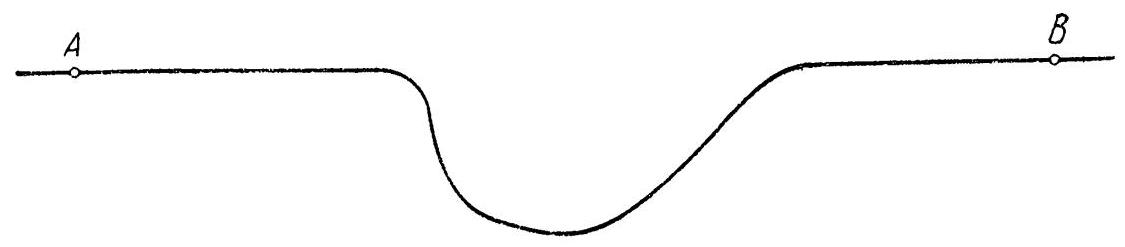
\includegraphics[max width=1.0\textwidth]{images/bo_d547imjef24c73bgfcdg_228_193_1252_1125_247_0.jpg}
\end{center}
\hspace*{3em}

Prac. 81.

Пусть, например, пункты А и В расположены на ровной местности, на которой между пунктами А и В имеется углубление (скажем, овраг, который дорога должна пересечь), так что разрез местности по линии AB имеет вид, изображенный на рис. 81. Мы будем считать изображенную на рис. 81 линию графиком функции \(y\left( t\right)\), предполагая, что ось абсцисс совпадает с прямой AB, а абсциссы точек А и В равны соответственно а и b. Стенки оврага мы предположим крутыми (имеющими уклон >α). Функцию, график которой представляет собой искомый профиль дороги, обозначим, как и выше,

\begin{center}
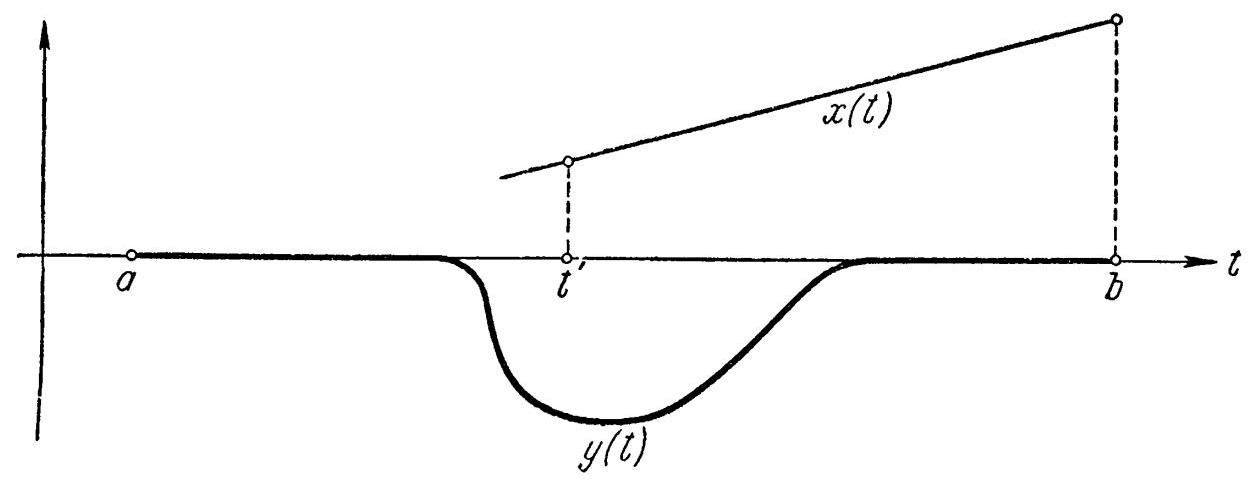
\includegraphics[max width=1.0\textwidth]{images/bo_d547imjef24c73bgfcdg_229_136_473_1256_482_0.jpg}
\end{center}
\hspace*{3em}

Pnc. 82.

через \(x\left( t\right)\). Легко видеть, что \(x\left( t\right)  \leq  0\) для всех t. Дей- ствительно, если х (и') > 0, то, в силу непрерывности

\begin{center}
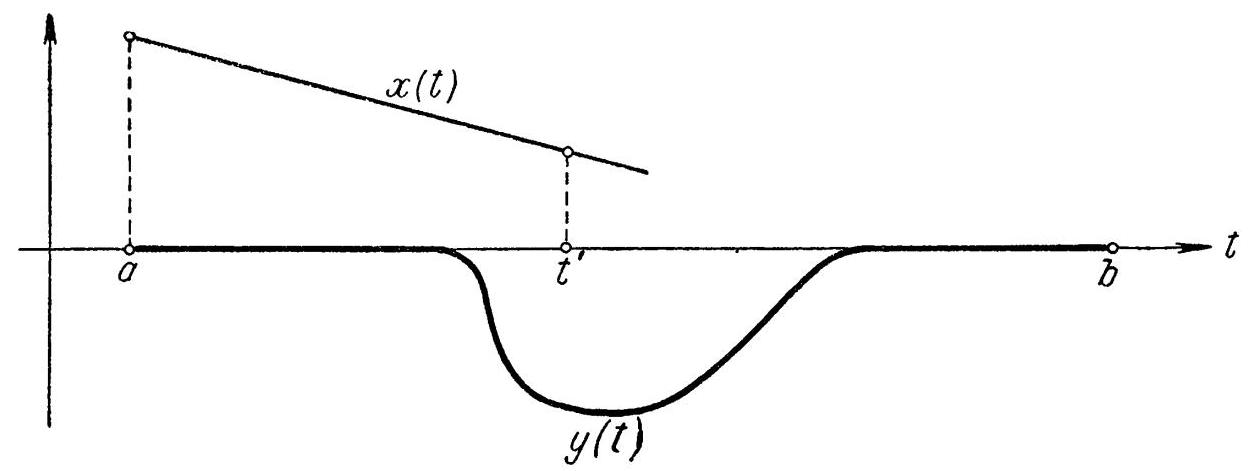
\includegraphics[max width=1.0\textwidth]{images/bo_d547imjef24c73bgfcdg_229_127_1243_1254_471_0.jpg}
\end{center}
\hspace*{3em}

Prac. 83.

функции \(x\left( t\right)\), неравенство \(x\left( t\right)  > 0\) будет иметь место и в некоторой окрестности точки г/. Поэтому, несколько сместив, если нужно, точку т’оны можем добиться выпол-

нения неравенств \(x\left( {t}^{\prime }\right)  > 0,{\int }_{a}^{{t}^{\prime }}\left( {x\left( t\right)  - y\left( t\right) }\right) {dt} \neq  0\). Если

HMEET MECTO HEPABEHCTBO \({\int }_{a}^{{t}^{\prime }}\left( {x\left( t\right)  - y\left( t\right) }\right) {dt} > 0\), TO,

в силу (27), \({x}^{\prime }\left( t\right)  =  + \alpha\) npu \(t \geq  {t}^{\prime }\) (рис. 82), u потому

\[
{\int }_{a}^{b}\left( {x\left( t\right)  - y\left( t\right) }\right) {dt} = {\int }_{a}^{{t}^{\prime }}\left( {x\left( t\right)  - y\left( t\right) }\right) {dt} + {\int }_{{t}^{\prime }}^{b}\left( {x\left( t\right)  - y\left( t\right) }\right) {dt} > 0,
\]

что противоречит соотношению (28). Если же имеет место неравенство \({\int }_{a}^{{t}^{\prime }}\left( {x\left( t\right)  - y\left( t\right) }\right) {dt} < 0\),то,в силу (27), \({x}^{\prime }\left( t\right)  = \; =  - \alpha\) npu \(t \leq  {t}^{\prime }\) (pnc. 83), a это означает,что \(x\left( t\right)  > y\left( t\right)\) при а \(\leq  t \leq  {t}^{\prime } -\) вопреки неравенству \({\int }_{a}^{{t}^{\prime }}\left( {x\left( t\right)  - y\left( t\right) }\right) {dt} < 0\).

\begin{center}
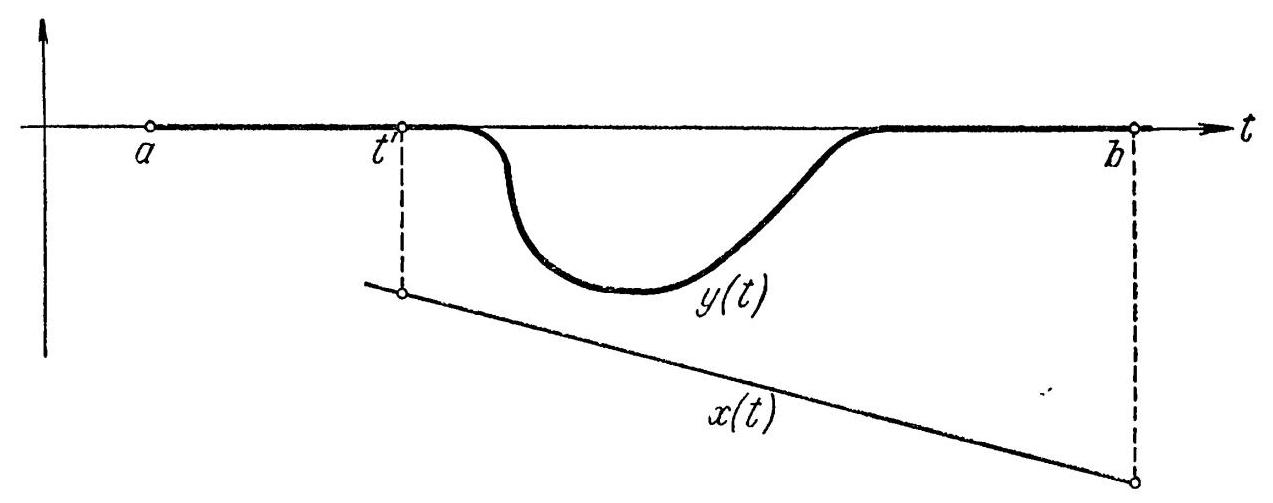
\includegraphics[max width=1.0\textwidth]{images/bo_d547imjef24c73bgfcdg_230_122_906_1273_503_0.jpg}
\end{center}
\hspace*{3em}

Рис. 84.

Полученное противоречие показывает, что \(x\left( t\right)  \leq  0\) для BCex \(t\).

Предположим теперь, что в некоторой точке t' выполнено неравенство \(x\left( {t}^{\prime }\right)  < y\left( {t}^{\prime }\right)\). Если при этом \({\int }_{0}^{{t}^{\prime }}\left( {x\left( t\right)  - y\left( t\right) }\right) {dt} < 0\), то при t > t’ дорога спускается c уклоном \(\alpha\) (т. е. \({x}^{\prime }\left( t\right)  =  - \alpha\) ) до тех пор,пока нера- венство \({\int }_{a}^{t}\left( {x\left( t\right)  - y\left( t\right) }\right) {dt} < 0\) не нарушается. При этом графики функций \(x\left( t\right)\) и \(y\left( t\right)\) обязательно должны пере- сечься при \(t \gg  {t}^{\prime }\),ибов противном случае мы имели бы

\(x\left( t\right)  < y\left( t\right)\) при всех t > t’ (рис. 84),и потому

\[
{\int }_{a}^{b}\left( {x\left( t\right)  - y\left( t\right) }\right) {dt} = {\int }_{a}^{{t}^{\prime }}\left( {x\left( t\right)  - y\left( t\right) }\right) {dt} + {\int }_{{t}^{\prime }}^{b}\left( {x\left( t\right)  - y\left( t\right) }\right) {dt} < 0
\]

вопреки соотношению (28). Аналогично, если выполнены неравенства \(x\left( {t}^{\prime }\right)  < y\left( {t}^{\prime }\right)\) и \({\int }_{a}^{{t}^{\prime }}\left( {x\left( t\right)  - y\left( t\right) }\right) {dt} > 0\),то при

\begin{center}
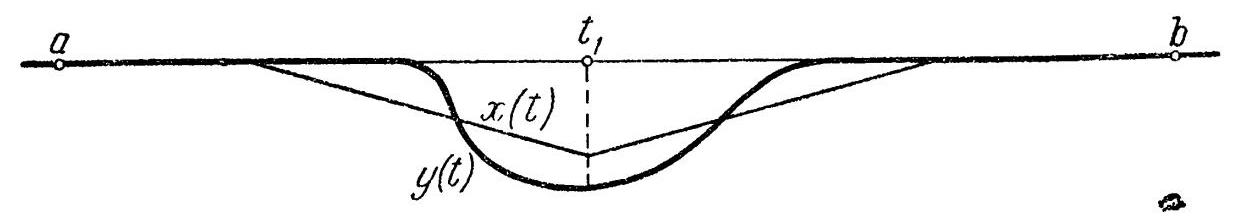
\includegraphics[max width=1.0\textwidth]{images/bo_d547imjef24c73bgfcdg_231_152_635_1234_217_0.jpg}
\end{center}
\hspace*{3em}

Pnc. 85.

\(t < {t}^{\prime }\) дорога подходит к точке \({t}^{\prime }\) ,поднимаясь с укло- ном α (т. е. \({x}^{\prime }\left( t\right)  =  + \alpha\) ),причем при \(t < {t}^{\prime }\) обязательно имеется точка пересечения графиков \(x\left( t\right)\) и \(y\left( t\right)\) .

\begin{center}
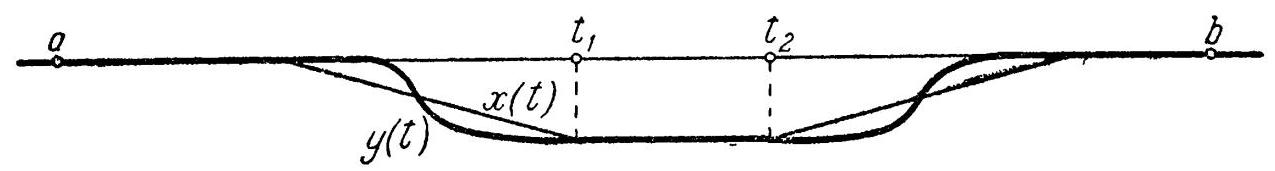
\includegraphics[max width=1.0\textwidth]{images/bo_d547imjef24c73bgfcdg_231_124_1161_1275_171_0.jpg}
\end{center}
\hspace*{3em}

Pnc. 86.

Bce сказанное позволяет отыскивать функцию \(x\left( t\right)\) для различных графиков у \(y\left( t\right)\). Примеры приведены на рис. 85, 86. При этом для определения точки и и зна- чения \(x\left( {t}_{1}\right)\) на рис. 85 мы имеем соотношения

\[
{\int }_{a}^{{t}_{1}}\left( {x\left( t\right)  - y\left( t\right) }\right) {dt} = 0,\;{\int }_{{t}_{1}}^{b}\left( {x\left( t\right)  - y\left( t\right) }\right) {dt} = 0,
\]

а для определения точек и и и и на рис. 86 имеем соот- ношения

\[
{\int }_{a}^{{t}_{1}}\left( {x\left( t\right)  - y\left( t\right) }\right) {dt} = 0,\;{\int }_{{t}_{2}}^{b}\left( {x\left( t\right)  - y\left( t\right) }\right) {dt} = 0.
\]

Разумеется, рассмотренные на приведенных рисунках случаи очень просты. Они были подробно изучены лишь c единственной целью — показать, что соотношений (26), (27), (28) (а в общем случае — соотношений, указанных в теореме 19), вообще говоря, «достаточно» для нахожде- ния искомой функции \(x\left( t\right)\).

\section*{§ 27. Оптимальные процессы с запаздыванием *)}

B ряде случаев задача оптимального управления осложняется эффектом запаздывания. Запаздывание может возникать в связи с затратой времени на передачу сигнала или, как это бывает чаще, вызывается упрощающими явление предположениями, в силу которых считают, что действие промежуточных и усиливающих звеньев в упра- вляемом объекте сводится к передаче сигнала с запазды- ванием. Довольно обширный круг технических задач этого рода укладывается в следующую математическую схему.

Движение объекта описывается в фазовом простран- стве X переменных \({x}^{1},\ldots,{x}^{n}\) системой уравнений

\[
\frac{d{x}^{i}\left( t\right) }{dt} = {f}^{i}\left( {{x}^{1}\left( t\right) ,\ldots ,{x}^{n}\left( t\right) ,{x}^{1}\left( {t - \theta }\right) ,\ldots ,{x}^{n}\left( {t - \theta }\right) ,u\left( t\right) }\right) ,
\]

\[
i = 1,\ldots ,n,\theta  = \text{ const } > 0, \tag{29}
\]

или, в векторной форме,

\[
\frac{{dx}\left( t\right) }{dt} = f\left( {x\left( t\right) ,x\left( {t - \theta }\right) ,u\left( t\right) }\right) . \tag{30}
\]

Таким образом, запаздывающий аргумент содержится только в фазовых координатах и отсутствует в управле- нии. Функции \({f}^{i}\left( {{x}^{1},\ldots,{x}^{n},{y}^{1},\ldots,{y}^{n},u}\right)\) предпола- гаются непрерывными по совокупности своих аргументов и непрерывно дифференцируемыми по \({x}^{1},\ldots,{x}^{n},{y}^{1},\ldots,{y}^{n}\). Иначе говоря, функции \({f}^{i},\frac{\partial {f}^{i}}{\partial {x}^{j}},\frac{\partial {f}^{i}}{\partial {y}^{j}}\) определены и непре- рывны на прямом произведении \(X \times  X \times  \overline{U}\). В качестве класса \(D\) допустимых управлений мы примем класс всех к у с о чн о - н е п р е р ы в н ы х управлений со значениями в U (или некоторый его подкласс); см.§ 10. Как и прежде, мы будем для определенности предполагать, что рассматриваемые управнения в точках разрыва непре- рывны слева

\[
u\left( t\right)  = u\left( {t - 0}\right) .
\]

\HRule

*) Результаты этого параграфа принадлежат Г.Л. Харатишвили

\HRule

Для однозначного определения траектории и(t) урав- нения (30) на отрезке бо ≤ t ≤ t, необходимо задать не только допустимое управление и(t), \({t}_{0} \leq  t \leq  {t}_{1}\),но и начальную функцию φ(t) со значениями в X, опреде- ленную на отрезке to — 0 ≤ t ≤ t0. Начальную функцию \(\varphi \left( t\right)\) мы будем предполагать непрерывной на всем отрезке \({t}_{0} - \theta  \leq  t \leq  {t}_{0}.\)

\(\Phi\) укцию \(x\left( t\right)\) ,3аданную на отрезке \({t}_{0} - \theta  \leq  t \leq  {t}_{1}\) и н е п р е р ы в н у ю н а в с е м э т о м о т р е з к е, мы будем называть траекторией уравнения (30), соответ- ствующей допустимому управлению \(u\left( t\right) ,{t}_{0} \leq  t \leq  {t}_{1}\) ,и за- данной начальной функции \(\varphi \left( t\right) ,{t}_{0} - \theta  \leq  t \leq  {t}_{0}\) , ecли функция \(x\left( t\right)\) на отрезке \({t}_{0} \leq  t \leq  {t}_{1}\) удовлетворяет уравне- нию (30), a на отрезке и - о мес не сво совпадает с функ- цией \(\varphi \left( t\right)\) .

Перейдем теперь к ф о р м у л и р о в к е оптимальной задачи, которую мы будем решать в этом параграфе. При этом мы сразу сформулируем задачу с подвижным правым концом (которая включает в себя, как частный случай, и задачу с закрепленным правым концом).

Пусть дана функция \({f}^{0}\left( {{x}^{1},\ldots,{x}^{n},{y}^{1},\ldots,{y}^{n},u}\right)\), удовлетворяющая тем же условиям, что и функции \({f}^{i}\), \(i = 1,\ldots,n.\Pi\) усть, кроме того, в X задано гладкое \(k\) -мерное многообразие \({S}_{1},0 \leq  k \leq  n - 1\),и начальная функция φ(t). Требуется в классе допустимых управле- ний выбрать такое управление \(u\left( t\right),{t}_{0} \leq  t \leq  {t}_{1}\),чтобы траектория \(x\left( t\right),{t}_{0} - \theta  \leq  t \leq  {t}_{1}\), системы (29), соответ- ствующая выбранному управлению и (и и заданной начальной функции q (t), удовлетворяла краевому условию \(x\left( {t}_{1}\right)  \in  {S}_{1}\) и интеграл

\[
{\int }_{{t}_{0}}^{{t}_{1}}{f}^{0}\left( {x\left( t\right) ,x\left( {t - \theta }\right) ,u\left( t\right) }\right) {dt} \tag{31}
\]

принимал минимальное значение. Заметим, что пределы интегрирования в (31) не фиксированы; фиксированы лишь «краевые» условия: \(\varphi \left( t\right)\) и \({S}_{1}\).

Если \({f}^{0} \equiv  1\),то мы получаем задачу об оптимальных быстродействиях для систем с запаздыванием.

Если размерность многообразия \({S}_{1}\) равна нулю, то оно превращается в точку, и мы получаем оптимальную задачу с закрепленным правым концом.

Дадим теперь другую (эквивалентную) формулировку нашей оптимальной задачи, более удобную для форму- лировки и доказательства основного результата.

Введем в рассмотрение (n + 1)-мерное фазовое про- странство \(X\) переменной \(x = \left( {{x}^{0},\ldots,{x}^{n}}\right)  = \left( {{x}^{0},x}\right)\) и обо- значим через \(L\) множество всех точек ( рых \(x \in  {S}_{1}\) (т. e. \(L\) есть многообразие размерности \(k + 1\), являющееся прямым произведением многообразия S1 на ось \(\left. {x}^{0}\right)\). Тогда наша оптимальная задача эквивалентна следующей задаче (cp. стр. 20).

Система уравнений движения фазовой точки x(t) = \(= \left( {{x}^{0}\left( t\right),\ldots,{x}^{n}\left( t\right) }\right)\) имеет вид

\[
\frac{d{x}^{i}\left( t\right) }{dt} = {f}^{i}\left( {x\left( t\right) ,x\left( {t - \theta }\right) ,u\left( t\right) }\right) ,i = 0,1,\ldots ,n, \tag{32}
\]

или, в векторной форме,

\[
\frac{{dx}\left( t\right) }{dt} = f\left( {x\left( t\right) ,x\left( {t - \theta }\right) ,u\left( t\right) }\right) . \tag{33}
\]

Требуется выбрать такое допустимое управление и(t), \({t}_{0} \leq  t \leq  {t}_{1}\),чтобы соответствующая этому управлению и начальной функции \(\varphi \left( t\right)  = \left( {0,\varphi \left( t\right) }\right),{t}_{0} - \theta  \leq  t \leq  {t}_{0}\), траектория \(x\left( t\right)  = \left( {{x}^{0}\left( t\right),x\left( t\right) }\right),{t}_{0} \leq  t \leq  {t}_{1}\), системы (32) удов- летворяла краевому условию \(x\left( {t}_{1}\right)  \in  L\) и при этом коор- дината \({x}^{0}\left( {t}_{1}\right)\) была минимальной.

Всякое допустимое управление \(u\left( t\right)\) и соответствующую траекторию х(t), удовлетворяющие сформулированным условиям, назовем оптимальными.

Для решения поставленной задачи, как и раньше, введем в рассмотрение вспомогательный вектор \(\psi  = \; = \left( {{\psi }_{0},\ldots,{\psi }_{n}}\right)\) u cocaabu скалярную функцию \(\mathcal{K} = \mathop{\sum }\limits_{{\alpha  = 0}}^{n}{\psi }_{\alpha }{f}^{\alpha } = {\left( \psi,f\right) }_{n}\) переменных \({\psi }_{0},\ldots,{\psi }_{n},{x}^{1},\ldots,{x}^{n}, \; {y}^{1},\ldots,{y}^{n},u\). Через \(\mathcal{M}\left( {\psi,x,y}\right)\) обозначим верхнюю грань значений функции Жпри фиксированных ф, х, у и при \(u\),меняющемся на множестве U.

Введем, далее, в рассмотрение следующие две системы уравнений для вспомогательных переменных \({\psi }_{0},{\psi }_{1},\ldots,{\psi }_{n}\) :

\[
\frac{d{\psi }_{i}\left( t\right) }{dt} =  - \frac{\partial \mathcal{K}\left( {\psi \left( t\right) ,x\left( t\right) ,x\left( {t - \theta }\right) ,u\left( t\right) }\right) }{\partial {x}^{i}} -
\]

\[
- \frac{\partial \mathcal{K}\left( {\psi \left( {t + \theta }\right) ,x\left( {t + \theta }\right) ,x\left( t\right) ,u\left( {t + \theta }\right) }\right) }{\partial {y}^{i}},i = 0,1,\ldots ,n;\left( {34}\right) \tag{34}
\]

\[
\frac{d{\psi }_{i}\left( t\right) }{dt} =  - \frac{\partial \mathcal{K}\left( {\psi \left( t\right) ,x\left( t\right) ,x\left( {t - \theta }\right) ,u\left( t\right) }\right) }{\partial {x}^{i}},
\]

\[
i = 0,1,\ldots ,n. \tag{35}
\]

Мы будем говорить, что система непрерывных кусочно- дифференцируемых на отрезке и «у функций цо(т), \({\psi }_{1}\left( t\right),\ldots,{\psi }_{n}\left( t\right)\) соответствует ф ункциям \(u\left( t\right),{t}_{0} \leq  t \leq  {t}_{1}\), If \(x\left( t\right),{t}_{0} - \theta  \leq  t \leq  {t}_{1}\), если на отрезке б, удовлетворяет системе (34), а на отрезке би — 0 е меня те ти е ти системе (35).

Теперь мы можем сформулировать н е о б х о д и м м о е условие оптимальности для поставленной задачи (в фор- ме принципа максимума).

T e o p e м a 20. Пусть и(t), то set ≤ t, - такое допус- тимое управление, что соответствующая ему траекто- рия \(x\left( t\right),{t}_{0} - \theta  \leq  t \leq  {t}_{1}\), систеты (32) с начальной функ- уией \(\varphi \left( t\right),{t}_{0} - \theta  \leq  t \leq  {t}_{0},\) проходит в некоторый момент \({t}_{1} > {t}_{0}\) через некоторую точку многообразия L. Для оптимальности управления и(t) и соответствующей траектории х(t) необходимо существование такой нену- левой вектор-функции \(\psi \left( t\right)  = \left( {{\psi }_{0}\left( t\right),{\psi }_{1}\left( t\right),\ldots,{\psi }_{n}\left( t\right) }\right)\), coom- ветствующей функциям и(t) и то:

\({1}^{ \circ  }\) для всех t, \({t}_{0} \leq  t \leq  {t}_{1}\) ,выполняется условие максимума \(\mathcal{K}\left( {\psi \left( t\right) ,x\left( t\right) ,x\left( {t - \theta }\right) ,u\left( t\right) }\right)  =\)

\[
= \mathcal{M}\left( {\psi \left( t\right) ,x\left( t\right) ,x\left( {t - \theta }\right) }\right) ; \tag{36}
\]

\({2}^{ \circ  }\) в конечный момент \({t}_{1}\) выполнены соотношения

\[
{\psi }_{0}\left( {t}_{1}\right)  \leq  0,\;\mathcal{M}\left( {\psi \left( {t}_{1}\right) ,x\left( {t}_{1}\right) ,x\left( {{t}_{1} - \theta }\right) }\right)  = 0 \tag{37}
\]

(заметим, что в силу уравнений (34), (35) мы имеем \({\psi }_{0} =\) const);

\({3}^{ \circ  }\) вектор \(\left( {{\psi }_{1}\left( {t}_{1}\right) ,\ldots ,{\psi }_{n}\left( {t}_{1}\right) }\right)\) opmooгонален касатель- ной плоскости многообразия в 1, проведенной в точке \(x\left( {t}_{1}\right)  = \left( {{x}^{1}\left( {t}_{1}\right) ,\ldots ,{x}^{n}\left( {t}_{1}\right) }\right) .\)

Заметим, что при применении этой теоремы возникает трудность, связанная с тем обстоятельством, что неиз- вестные функции \({x}^{1}\left( t\right)\), \(\ldots\), \({x}^{n}\left( t\right)\), \({\psi }_{1}\left( t\right)\), \(\ldots\), \({\psi }_{n}\left( t\right)\) входят в систему (32), (34) как с запаздывающим, так и с опережающим аргументом. Для линейных систем эта трудность, очевидно, отсутствует.

В случае оптимальности по быстродействию ( вместо функции Жрассматривается функция \(H = \mathop{\sum }\limits_{{\alpha  = 1}}^{n}{\psi }_{\alpha }{f}^{\alpha }\) переменных \({\psi }_{1},\ldots,{\psi }_{n},{x}^{1},\ldots,{x}^{n}{y}^{1},\ldots,{y}^{n},v\) ; верх- няя грань значений этой функции по и € U (при фикси- рованных \(\psi,x,y\) ) обозначается через \(M\left( {\psi,x,y}\right)\). Заменяя в уравнениях (34), (35) функцию Ж функцией H, мы сможем и в этом случае определить функции \({\psi }_{1}\left( t\right)\),... \(\ldots,{\psi }_{n}\left( t\right),{t}_{0} \leq  t \leq  {t}_{1}\), соотве стовующие функциям \(u\left( t\right)\), \({t}_{0} \leq  t \leq  {t}_{1}\), if \(x\left( t\right),{t}_{0} - \theta  \leq  t \leq  {t}_{1}\). После этого для случая оптимальных быстродействий сохраняется формулировка теоремы 20 с той только разницей, что функции Ж и М заменяются функциями H и M, а условие 2 \textdegree  заменяется условием

\[
\mathcal{M}\left( {\psi \left( {t}_{1}\right) ,x\left( {t}_{1}\right) ,x\left( {{t}_{1} - \theta }\right) }\right)  \geq  0.
\]

Иначе говоря, условие оптимальности по быстродействию вытекает из теоремы 20 совершенно таким же образом, как теорема 2 получается из теоремы 1.

До ка за т е л ь с т в о теоремы 20 в общих чертах проводится по той же схеме, что и доказательство теоремы 1 (или теоремы 8). Мы проведем его, подробно отмечая те части доказательства, в которых необходимо произвести некоторые изменения, и опуская построения, ничем не отличающиеся от изложенных в главе 2.

Пусть \(x\left( t\right)\) — решение уравнения (33), соответствующее допустимому управлению \(u\left( t\right),{t}_{0} \leq  t \leq  {t}_{1}\),и начальной функции \(\varphi \left( t\right),{t}_{0} - \theta  \leq  t \leq  {t}_{0}\). Системой уравнений в вариа- циях для системы (32) назовем следующую линейную систему:

\[
\frac{d\left( {\delta {x}^{i}\left( t\right) }\right) }{dt} = \mathop{\sum }\limits_{{\alpha  = 0}}^{n}\left( {\frac{\partial {f}^{i}\left( {x\left( t\right) ,x\left( {t - \theta }\right) ,u\left( t\right) }\right) }{\partial {x}^{\alpha }}\delta {x}^{\alpha }\left( t\right)  + }\right.
\]

\[
\left. {+\frac{\partial {f}^{i}\left( {x\left( t\right) ,x\left( {t - \theta }\right) ,u\left( t\right) }\right) }{\partial {y}^{\alpha }}\delta {x}^{\alpha }\left( {t - \theta }\right) }\right) ,\;i = 0,1,\ldots ,n.(3 \tag{38}
\]

(38)на отрезке б ш м но н и н и н а его части, которые соот- ветствуют к у с о ч н о - н е п р е р ы в н ы м начальным функциям; так как мы здесь не исключаем возможности разрыва решения в начальный момент \({t}_{0}\),то для одно- значного определения решения системы (38) необходимо задать (кроме начальной функции) начальное значение этого решения. Таким образом, если η(t) — произвольная кусочно-непрерывная функция, заданная на отрезке \(\tau  - \theta  \leq  t \leq  \tau\),где \(\tau  \in  \left\lbrack  {{t}_{0},{t}_{1}}\right\rbrack\), a \(\xi  -\) произвольный век- тор пространства X, то решением системы (38) с начальной функцией η(t) и начальным значением ξ мы будем назы- вать такую функцию \({\delta x}\left( t\right)  = \left( {\delta {x}^{0}\left( t\right),\delta {x}^{1}\left( t\right),\ldots,\delta {x}^{n}\left( t\right) }\right)\), \(\tau  - \theta  \leq  t \leq  {t}_{1}\),которая на промежутке \(\tau  - \theta  \leq  t \leq  \tau\) cos- падает с \(\eta \left( t\right)\),на отрезке \(\tau  \leq  t \leq  {t}_{1}\) непрерывна и удов- летворяет системе (38) и, кроме того, удовлетворяет соот- ношению \({\delta x}\left( \tau \right)  = \xi\). Это решение мы будем обозначать символом \({A}_{t,\tau }\left( {\eta,\xi }\right),\tau  - \theta  \leq  t \leq  {t}_{1}\).

Мы условимся (при \(\tau  - \theta  \leq  t \leq  {t}_{1}\) ) считать \({A}_{t,\tau }\left( {\eta,\xi }\right)\) с в я з а н н ы м вектором, исходящим из точки х (н. ) Ta- ким образом, при заданных начальных элементах ξ и η(t), \(\tau  - \theta  \leq  t \leq  \tau\), определяется векторное поле \({A}_{t,\tau }\left( {\eta,\xi }\right)\), \(\tau  - \theta  \leq  t \leq  {t}_{1}\) ; мы будем говорить, что векторы \({A}_{t,\tau }\left( {\eta,\xi }\right)\) этого поля получаются друг из друга переносом вдоль траектории \(x\left( t\right)\).

Отметим следующие легко доказываемые свойства переноса, которые нам понадобятся в дальнейшем (ср. формулы (17) гл. 2).

I. \({A}_{{t}_{0},{t}_{0}}\left( {\eta,\xi }\right)  = \xi\).

II. Положим \({\eta }_{1}\left( t\right)  = {\mathrm{A}}_{t,\tau }\left( {\eta,\xi }\right),{\tau }_{1} - \theta  \leq  t \leq  {\tau }_{1}\),где \({t}_{0} \leq  \tau  \leq  {\tau }_{1} \leq  {t}_{1}\) ; тогда

\[
{A}_{t,{\tau }_{1}}\left( {{\eta }_{1},{A}_{{\tau }_{1},\tau }\left( {\eta ,\xi }\right) }\right)  = {A}_{t,\tau }\left( {\eta ,\xi }\right) ,\;{\tau }_{1} \leq  t \leq  {t}_{1}.
\]

\[
\text{ III. }{A}_{t,\tau }\left( {{\gamma }_{1}{\eta }_{1} + {\gamma }_{2}{\eta }_{2},{\gamma }_{1}{\xi }_{1} + {\gamma }_{2}{\xi }_{2}}\right)  =
\]

\[
= {\gamma }_{1}{A}_{t,\tau }\left( {{\eta }_{1},{\xi }_{1}}\right)  + {\gamma }_{2}{A}_{t,\tau }\left( {{\eta }_{2},{\xi }_{2}}\right) ,\tau  - \theta  \leq  t \leq  {t}_{1},
\]

где \({\gamma }_{1}\) и \({\gamma }_{2}\) — произвольные действительные числа.

IV. Пусть \({\eta }_{1}\left( t\right)\) — некоторая кусочно-непрерывная функ- ция, заданная на отрезке τ — θ ≤ t ≤ τ (где τ ∈ [t, t]), \(M\) - некоторая константа и ξ - произвольный вектор. Пусть, далее, полуинтервалы \({I}_{i}\) определяются так же, как и в \$ 13, а т(t) — функция, определенная на отрезке \(\tau  - \theta  \leq  t \leq  \tau\) следующим образом:

\[
\left\{  \begin{array}{l} \eta \left( t\right)  = \varepsilon {\eta }_{1}\left( t\right)  + o\left( \varepsilon \right) \text{ вовсехточкахотрезхатрезхат-θ } \leq  t \leq  \tau , \\  \eta \left( t\right)  \mid   \leq  {\varepsilon M}\text{ наллналлежапих полуинтервала }{I}_{i}. \end{array}\right.
\]

Torja

\[
{A}_{t,\tau }\left( {\eta ,{\varepsilon \xi } + o\left( \varepsilon \right) }\right)  = {A}_{t,\tau }\left( {\varepsilon {\eta }_{1},{\varepsilon \xi }}\right)  + o\left( \varepsilon \right) ,\tau  \leq  t \leq  {t}_{1}.
\]

Свойства I и II непосредственно вытекают из опреде- ления символа А \({t}_{k,\tau }\left( {\eta,\xi }\right)\). Справедливость свойства III на отрезке б 10 мест. в об чекает из того, что на этом отрезке система (38) представляет собой линейную (неод- нородную) систему о б ы к н о в е н н ы х дифференциаль- ных уравнений. На последующих отрезках длины 0 (вплоть до \({t}_{1}\) ) свойство III можно доказать совершенно анало- гично, воспользовавшись свойством II. Таким же образом устанавливается и справедливость свойства IV.

Перейдем теперь к в а р и а ц и я м у п р а в л е н и й и трае к т о р и й. Пусть \(u\left( t\right),{t}_{0} \leq  t \leq  {t}_{1}\),— допусти- мое управление, а х(t) — соответствующая ему траектория уравнения (33) с начальной функцией q(t), \({t}_{0} - \theta  \leq  t \leq  {t}_{0}\). Правильными точками управления \(u\left( t\right)\) будут все точки его непрерывности, т. е. все, кроме конечного числа, точки от- резка \({t}_{0} \leq  t \leq  {t}_{1}\). Мы условимся всякое управление и(t), \({t}_{0} \leq  t \leq  {t}_{1}\),продолжать за точку \({t}_{1}\),полагая \(u\left( t\right)  = u\left( {t}_{1}\right)\) при \(t > {t}_{1}\). Важно отметить, что при этом точка \({t}_{1}\) будет правильной точкой управления \(u\left( t\right)\). Если т — произволь- ная точка непрерывности управления \(u\left( t\right)\), то, каковы бы ни были действительные числа р и q, имеет место соот- ношение

\[
\mathop{\int }\limits_{{\tau  + {p\varepsilon }}}^{{\tau  + {q\varepsilon }}}f\left( {x\left( t\right) ,x\left( {t - \theta }\right) ,u\left( t\right) }\right) {dt} =
\]

\[
= \varepsilon \left( {q - p}\right) f\left( {x\left( \tau \right) ,x\left( {\tau  - \theta }\right) ,u\left( \tau \right) }\right)  + o(\varepsilon \tag{39}
\]

(cp. формулу (1) гл. 2).

Пусть теперь \(u\left( t\right)\), \({t}_{0} \leq  t \leq  {t}_{1}\),-допустимое управле- ние, \(x\left( t\right)\) — соответствующая траектория уравнения (33) с начальной функцией \(\varphi \left( t\right),{t}_{0} - \theta  \leq  t \leq  {t}_{0}\), a \(\mathfrak{a} -\) символ, определяющий варьирование управления. Проварьирован- ное управление обозначим через и*(t), а соответствующую этому управлению траекторию с т о й же начальной функцией q(t) обозначим через x*(t). (Отметим, что при любом в е 30 траектория — хри представляет собой н е п р е р ы в н у ю функцию от t в силу определения решений уравнения (33).) При достаточно малом \& траек- тория \({x}^{ * }\left( t\right)\) определена на всем отрезке б, сен сею- рема о непрерывной зависимости решения от параметров). Покажем, что для любой точки τ непрерывности управ- ления и(t) имеет место следующая формула (ср. формулы (21), (22) гл. 2):

\[
{x}^{ * }\left( {\tau  + {\varepsilon \delta t}}\right)  = x\left( \tau \right)  + {\varepsilon \Delta x} + o\left( \varepsilon \right) , \tag{40}
\]

где \({\Delta x}\) - не зависящий от ε вектор, определяемый фор- мулой:

\[
{\Delta x} = f\left( {x\left( \tau \right) ,x\left( {\tau  - \theta }\right) ,u\left( \tau \right) }\right) {\delta t} +
\]

\[
+ \mathop{\sum }\limits_{{i = 1}}^{s}{A}_{\tau ,{\tau }_{i}}\left( {0,f\left( {x\left( {\tau }_{i}\right) ,x\left( {{\tau }_{i} - \theta }\right) ,{v}_{i}}\right)  - }\right.
\]

\[
\left. {-f\left( {x\left( {\tau }_{i}\right) ,x\left( {{\tau }_{i} - \theta }\right) ,u\left( {\tau }_{i}\right) }\right) }\right) \delta {t}_{i}\text{ . } \tag{41}
\]

Доказательство формул (40), (41) аналогично выводу формул (21), (22) в гл. 2. Прежде всего заметим, что имеют место формулы

\[
x\left( {\tau  + {\varepsilon \delta t}}\right)  = x\left( \tau \right)  + {\varepsilon f}\left( {x\left( \tau \right) ,x\left( {\tau  - \theta }\right) ,u\left( \tau \right) }\right) {\delta t} + o\left( \varepsilon \right) ,\left( {42}\right) \tag{42}
\]

\[
{x}^{ * }\left( {\tau  + {\varepsilon \delta t}}\right)  = {x}^{ * }\left( \tau \right)  + {\varepsilon f}\left( {x\left( \tau \right) ,x\left( {\tau  - \theta }\right) ,u\left( \tau \right) }\right) {\delta t} + o\left( \varepsilon \right) \left( {43}\right) \tag{43}
\]

\[
\text{ (при }{\tau }_{s} < \tau \text{ ). }
\]

Эти формулы устанавливаются так же, как и фор- мулы (23), (25) гл. 2 (с заменой ссылки на формулу (1) гл. 2 ссылкой на указанную выше формулу (39)). Далее, совершенно так же, как и в гл. 2, находится приращение функции \({x}^{ * }\left( t\right)\) на полуинтервале \({I}_{i}\) :

\[
{\left. {x}^{ * }\right| }_{{I}_{i}} = {\varepsilon f}\left( {x\left( {\tau }_{i}\right) ,x\left( {{\tau }_{i} - \theta }\right) ,{v}_{i}}\right) \delta {t}_{i} + o\left( \varepsilon \right) \tag{44}
\]

(cp. формулу (26) гл. 2).

Переходим к индуктивной проверке соотношений (40), (41). \(\Pi\) pu \(s = 0\) эти формулы справедливы (см. (42)). Предположим, что они доказаны для случая, когда число полуинтервалов \({I}_{1},{I}_{2},\ldots\) меньше чем s, и докажем справедливость этих формул при наличии s полуинтер- валов \({I}_{1},{I}_{2},\ldots,{I}_{s}\). Обозначим через к такое цслое число, что

\[
{\tau }_{k + 1} = {\tau }_{k + 2} = \ldots  = {\tau }_{s}\text{ и }{\tau }_{i} < {\tau }_{s}\text{ при }i \leq  k
\]

(случай \(k = 0\) не исключается). Заменяя точку т точ- кой \({\tau }_{s}\),число бт - числом \({l}_{k + 1}\), a число s - меньшим чис- лом k, мы, в силу индуктивного предположения, получим из (40), (41)

\[
{x}^{ * }\left( {{\tau }_{s} + \varepsilon {l}_{k + 1}}\right)  = x\left( {\tau }_{s}\right)  + {\varepsilon f}\left( {x\left( {\tau }_{s}\right) ,x\left( {{\tau }_{s} - \theta }\right) ,u\left( {\tau }_{s}\right) }\right) {l}_{k + 1} +
\]

\[
+ \varepsilon \mathop{\sum }\limits_{{i = 1}}^{k}{A}_{{\tau }_{s,}{\tau }_{i}}\left( {0,f\left( {x\left( {\tau }_{i}\right) ,x\left( {{\tau }_{i} - \theta }\right) ,{v}_{i}}\right)  - }\right.
\]

\[
\left. {-f\left( {x\left( {\tau }_{i}\right) ,x\left( {{\tau }_{i} - \theta }\right) ,u\left( {\tau }_{i}\right) }\right) }\right) \delta {t}_{i} + o\left( \varepsilon \right) . \tag{45}
\]

Это есть значение функции \({x}^{ * }\left( t\right)\) в левом конце полу- интервала \({I}_{k + 1}\). Далее, так как полуинтервалы \({I}_{k + 1},\ldots,{I}_{s}\) примыкают один к другому, то, суммируя соотноше- ния (44) для \(i = k + 1,\ldots,s\) и складывая полученное соотношение с соотношением (45), найдем

\[
{x}^{ * }\left( {{\tau }_{s} + \varepsilon \left( {{l}_{s} + \delta {t}_{s}}\right) }\right)  =
\]

\[
= x\left( {\tau }_{s}\right)  + {\varepsilon f}\left( {x\left( {\tau }_{s}\right) ,x\left( {{\tau }_{s} - \theta }\right) ,u\left( {\tau }_{s}\right) }\right) \left( {{l}_{k + 1} + \delta {t}_{k + 1} + \ldots  + \delta {t}_{s}}\right)  +
\]

\[
+ \varepsilon \mathop{\sum }\limits_{{i = 1}}^{s}{A}_{{\tau }_{s},{\tau }_{i}}\left( {0,f\left( {x\left( {\tau }_{i}\right) ,x\left( {{\tau }_{i} - \theta }\right) ,{v}_{i}}\right)  - }\right.
\]

\[
\left. {-f\left( {x\left( {\tau }_{i}\right) ,x\left( {{\tau }_{i} - \theta }\right) ,{u}_{i}\left( {\tau }_{i}\right) }\right) }\right) \delta {t}_{i} + o \tag{46}
\]

(ср. вывод формулы (28) в гл. 2; при этом ссылка на пер- вую из формул (17) гл. 2 заменяется ссылкой на свой- ство I операции переноса, см. стр. 238). Если тьл ть то то соотношение (46) совпадает с (40), (41). Если же \({\tau }_{s} < \tau,\) то

\[
{l}_{s} + \delta {t}_{s} = 0,\;{l}_{k + 1} + \delta {t}_{k + 1} + \ldots  + \delta {t}_{s} = 0,
\]

и соотношение (46) принимает вид

\[
{x}^{ * }\left( {\tau }_{s}\right)  = x\left( {\tau }_{s}\right)  + \varepsilon \mathop{\sum }\limits_{{i = 1}}^{s}{A}_{{\tau }_{s},{\tau }_{i}}\left( {0,f\left( {x\left( {\tau }_{i}\right) ,x\left( {{\tau }_{i} - \theta }\right) ,{v}_{i}}\right)  - }\right.
\]

\[
\left. {-f\left( {x\left( {\tau }_{i}\right) ,x\left( {{\tau }_{i} - \theta }\right) ,u\left( {\tau }_{i}\right) }\right) }\right) \delta {t}_{i} + o\left( \varepsilon \right) \;\left( {{\tau }_{s} < \tau }\right) . \tag{47}
\]

Обозначим через \(\eta \left( t\right)\) функцию \({x}^{ * }\left( t\right)  - x\left( t\right)\), рассматри- ваемую на отрезке \({\tau }_{s} - \theta  \leq  t \leq  {\tau }_{s}\). Тогда (так как на от- резке \({\tau }_{s} \leq  t \leq  \tau\) управление \({u}^{ * }\left( t\right)\) совпадает c \(u\left( t\right) )\) функ- ция \({x}^{ * }\left( t\right)  - x\left( t\right)\) c точностью до \(o\left( \varepsilon \right)\) является на отрезке \({\tau }_{s} - \theta  \leq  t \leq  \tau\) ретением системы уравнений в вариа- циях (38) с начальной функцией η(t) и начальным значением \({x}^{ * }\left( {\tau }_{s}\right)  - x\left( {\tau }_{s}\right)\) (напомним, что обе функции \(x\left( t\right),{x}^{ * }\left( t\right)\) непрерывны). Иначе говоря, с точностью до \(o\left( \varepsilon \right)\) векторы \({x}^{ * }\left( t\right)  - x\left( t\right)\) получаются друг из друга (на orpe3ke \({\tau }_{s} - \theta  \leq  t \leq  \tau\) ) c tromonizio repenoca:

\[
{x}^{ * }\left( t\right)  - x\left( t\right)  = {A}_{t,{\tau }_{s}}\left( {\eta ,{x}^{ * }\left( {\tau }_{s}\right)  - x\left( {\tau }_{s}\right) }\right)  + o\left( \varepsilon \right) ,
\]

\[
{\tau }_{s} - \theta  \leq  t \leq  \tau \tag{48}
\]

Всюду, кроме конечного числа отрезков \({I}_{i}\), функция \(\eta \left( t\right)\), \({\tau }_{s} - \theta  \leq  t \leq  {\tau }_{s}\), имеет (в силу предположения индук- ции) вид

\[
\eta \left( t\right)  = {x}^{ * }\left( t\right)  - x\left( t\right)  = \varepsilon \mathop{\sum }\limits_{{i = 1}}^{k}{A}_{l,{\tau }_{i}}\left( {0,f\left( {x\left( {\tau }_{i}\right) ,x\left( {{\tau }_{i} - \theta }\right) ,{v}_{i}}\right)  - }\right.
\]

\[
\left. {-f\left( {x\left( {\tau }_{i}\right) ,x\left( {{\tau }_{i} - \theta }\right) ,u\left( {\tau }_{i}\right) }\right) }\right) \delta {t}_{i} + o\left( \varepsilon \right) \text{ . }
\]

Поэтому, в силу свойства IV (стр. 238—239), мы можем заменить формулу (48) формулой

\[
{x}^{ * }\left( t\right)  - x\left( t\right)  = {A}_{t,{\tau }_{s}}\left( {{\eta }_{1},{\xi }_{1}}\right)  + o\left( \varepsilon \right) ,{\tau }_{s} \leq  t \leq  \tau , \tag{49}
\]

где

\[
{\eta }_{1}\left( t\right)  = \varepsilon \mathop{\sum }\limits_{{i = 1}}^{k}{A}_{t}{\tau }_{i}\left( {0,f\left( {x\left( {\tau }_{i}\right) ,x\left( {{\tau }_{i} - \theta }\right) ,{v}_{i}}\right)  - }\right.
\]

\[
\left. {-f\left( {x\left( {\tau }_{i}\right) ,x\left( {{\tau }_{i} - \theta }\right) ,u\left( {\tau }_{i}\right) }\right) }\right) \delta {t}_{i}
\]

\[
{\xi }_{1} = \varepsilon \mathop{\sum }\limits_{{i = 1}}^{s}{A}_{{\tau }_{s},{\tau }_{i}}\left( {0,f\left( {x\left( {\tau }_{i}\right) ,x\left( {{\tau }_{i} - \theta }\right) ,{v}_{i}}\right)  - }\right.
\]

\[
\left. {-f\left( {x\left( {\tau }_{i}\right) ,x\left( {{\tau }_{i} - \theta }\right) ,u\left( {\tau }_{i}\right) }\right) }\right) \delta {t}_{i}
\]

(см. (47)). В силу свойства III операции переноса (стр. 238) мы можем формулу (49) переписать в виде

\[
{x}^{ * }\left( t\right)  - x\left( t\right)  = \varepsilon \mathop{\sum }\limits_{{i = 1}}^{k}{A}_{t,{\tau }_{s}}\left( {{\eta }_{1}^{\left( i\right) },{\xi }_{1}^{\left( i\right) }}\right) \delta {t}_{i} +
\]

\[
+ \varepsilon \mathop{\sum }\limits_{{i = k + 1}}^{s}{A}_{t,{\tau }_{s}}\left( {0,{\xi }_{1}^{\left( i\right) }}\right) \delta {t}_{i} + o\left( \varepsilon \right) ,{\tau }_{s} \leq  t \leq  \tau , \tag{50}
\]

где

\[
{\eta }_{1}^{\left( i\right) }\left( t\right)  = {A}_{t,{\tau }_{i}}\left( {0,f\left( {x\left( {\tau }_{i}\right) ,x\left( {{\tau }_{i} - \theta }\right) ,{v}_{i}}\right)  - }\right.
\]

\[
\left. {-f\left( {x\left( {\tau }_{i}\right) ,x\left( {{\tau }_{i} - \theta }\right) ,u\left( {\tau }_{i}\right) }\right) }\right) ,{\tau }_{s} - \theta  \leq  t \leq  {\tau }_{s},\;i = 1,\ldots ,k,
\]

\[
{\xi }_{1}^{\left( i\right) } = {A}_{{\tau }_{s},{\tau }_{i}}\left( {0,f\left( {x\left( {\tau }_{i}\right) ,x\left( {{\tau }_{i} - \theta }\right) ,{v}_{i}}\right)  - }\right.
\]

\[
\left. {-f\left( {x\left( {\tau }_{i}\right) ,x\left( {{\tau }_{i} - \theta }\right) ,u\left( {\tau }_{i}\right) }\right) }\right) ,\;i = 1,\ldots ,s.
\]

Наконец, в силу свойства II операции переноса (стр. 238) мы получаем

\[
{A}_{l,{\tau }_{s}}\left( {{\eta }_{1}^{\left( i\right) },{\xi }_{1}^{\left( i\right) }}\right)  = {A}_{t,{\tau }_{i}}\left( {0,f\left( {x\left( {\tau }_{i}\right) ,x\left( {{\tau }_{i} - \theta }\right) ,{v}_{i}}\right)  - }\right.
\]

\[
\left. {-f\left( {x\left( {\tau }_{i}\right) ,x\left( {{\tau }_{i} - \theta }\right) ,u\left( {\tau }_{i}\right) }\right) }\right) ,\;i = 1,\ldots ,k,
\]

a в сплу свойства I

\[
{\xi }_{1}^{i} = f\left( {x\left( {\tau }_{i}\right) ,x\left( {{\tau }_{i} - \theta }\right) ,{v}_{i}}\right)  -
\]

\[
- f\left( {x\left( {\tau }_{i}\right) ,x\left( {{\tau }_{i} - \theta }\right) ,u\left( {\tau }_{i}\right) }\right) ,\;i = k + 1,\ldots ,s.
\]

Таким образом, формула (50) принимает вид

\[
{x}^{ * }\left( t\right)  - x\left( t\right)  = \varepsilon \mathop{\sum }\limits_{{i = 1}}^{s}{A}_{t,{\tau }_{i}}\left( {0,f\left( {x\left( {\tau }_{i}\right) ,x\left( {{\tau }_{i} - \theta }\right) ,{v}_{i}}\right)  - }\right.
\]

\[
\left. {-f\left( {x\left( {\tau }_{i}\right) ,x\left( {{\tau }_{i} - \theta }\right) ,u\left( {\tau }_{i}\right) }\right) }\right) \delta {t}_{i} + o\left( \varepsilon \right) ,{\tau }_{s} \leq  t \leq  \tau .
\]

B частности, при \(t = \tau\),

\[
{x}^{ * }\left( \tau \right)  - x\left( \tau \right)  = \varepsilon \mathop{\sum }\limits_{{i = 1}}^{s}{A}_{\tau ,{\tau }_{i}}\left( {0,f\left( {x\left( {\tau }_{i}\right) ,x\left( {{\tau }_{i} - \theta }\right) ,{v}_{i}}\right)  - }\right.
\]

\[
\left. {-f\left( {x\left( {\tau }_{i}\right) ,x\left( {{\tau }_{i} - \theta }\right) ,u\left( {\tau }_{i}\right) }\right) }\right) \delta {t}_{i} + o\left( \varepsilon \right) .
\]

Складывая это соотношение с соотношением (43), мы и в этом случае (т. е. при т.е сто получаем соотноше- ния (40), (41), что и завершает индукцию. Тем самым, формулы (40), (41) полностью доказаны.

Так как \({t}_{1}\) - правильная точка управления \(u\left( t\right)\), то формулы (40),(41) применимы,в частности, при \(\tau  = {t}_{1}\) :

\[
{x}^{ * }\left( {{t}_{1} + {\varepsilon \delta t}}\right)  = x\left( {t}_{1}\right)  + {\varepsilon \Delta x} + o\left( \varepsilon \right) , \tag{51}
\]

где

\[
{\Delta x} = f\left( {x\left( {t}_{1}\right) ,x\left( {{t}_{1} - \theta }\right) ,u\left( {t}_{1}\right) }\right) {\delta t} +
\]

\[
+ \mathop{\sum }\limits_{{i = 1}}^{s}{A}_{{t}_{1},{\tau }_{i}}\left( {0,f\left( {x\left( {\tau }_{i}\right) ,x\left( {{\tau }_{i} - \theta }\right) ,{v}_{i}}\right)  - }\right.
\]

\[
\left. {-f\left( {x\left( {\tau }_{i}\right) ,x\left( {{\tau }_{i} - \theta }\right) ,u\left( {\tau }_{i}\right) }\right) }\right) \delta {t}_{i}. \tag{52}
\]

Обозначим теперь через \(K\) множество всех векто- ров (52), исходящих из точки х и холовно так же, как в главе 2 (стр. 105—110), устанавливается, что K — в ы п у к л ы й к о н у с пространства Х и что имеет мес- то лемма 3 (при т е ты. Справедлива также и лемма 4 для \(\tau  = {t}_{1}\),что следует непосредственно из леммы 3. Таким образом, если траектория \(x\left( t\right)\) оптимальна, то конус \(K\) не содержит внутри себя луча \({L}_{{t}_{1}}\). Поэтому через вер- шину \(x\left( {t}_{1}\right)\) конуса K можно провести такую гиперплос- кость \(\Gamma\),что конус K расположен в одном из двух замкну- тых полупространств, определяемых гиперплоскостью Г, а луч L, \({L}_{{t}_{1}} -\) в другом. (Конус к здесь заменяет пре- дельный конус, рассмотренный на стр. 118.) Это позво- ляет, как и в главе 2, определить нетривиальное реше- ние \(\psi \left( t\right)  = \left( {{\psi }_{0}\left( t\right),{\psi }_{1}\left( t\right),\ldots,{\psi }_{n}\left( t\right) }\right)\) системы уравнений (34), (35), для которого выполнены соотношения

\[
{\psi }_{0} = \text{ const } \leq  0, \tag{53}
\]

\[
\left( {\psi \left( {t}_{1}\right) ,{\Delta x}}\right)  \leq  0\text{ при }{\Delta x} \in  K. \tag{54}
\]

Докажем, что ψ(t) — аскомая функция (существо- вание которой утверждается в теореме 20). Пусть ти — произвольная правильная точка, т. е. точка непрерыв- ности управления \(u\left( t\right),{t}_{0} < {\tau }_{1} < {t}_{1}\). Рассмотрим символ а (см. § 14) с единственной точкой та ти (т. е. \(s = 1\) ) и с чис- лами \(\delta {t}_{1},{\delta t}\), соответственно равными единице и нулю. Тогда вектор \({\Delta x}\) (см. (52)), соответствующий этому сим- волу а, будет иметь значение

\[
{\Delta x} = {A}_{{t}_{1},{\tau }_{1}}\left( {0,f\left( {x\left( {\tau }_{1}\right) ,x\left( {{\tau }_{1} - \theta }\right) ,{v}_{1}}\right)  - }\right.
\]

\[
\left. {-f\left( {x\left( {\tau }_{1}\right) ,x\left( {{\tau }_{1} - \theta }\right) ,u\left( {\tau }_{1}\right) }\right) }\right) \text{ . } \tag{55}
\]

Положим

\[
g\left( t\right)  = {A}_{t,{\tau }_{1}}\left( {0,f\left( {x\left( {\tau }_{1}\right) ,x\left( {{\tau }_{1} - \theta }\right) ,{v}_{1}}\right)  - }\right.
\]

\[
\left. {-f\left( {x\left( {\tau }_{1}\right) ,x\left( {{\tau }_{1} - \theta }\right) ,u\left( {\tau }_{1}\right) }\right) }\right) ,\;{\tau }_{1} - \theta  \leq  t \leq  {t}_{1}.
\]

Тогда, по определению, \(g\left( t\right)  = \left( {{g}^{0}\left( t\right),{g}^{1}\left( t\right),\ldots,{g}^{n}\left( t\right) }\right)\) есть решение системы (38), соответствующее начальной функции, тождественно равной нулю (на отрезке \({\tau }_{1} - \theta  \leq  t \leq  {\tau }_{1}\) ) и начальному значению

\[
g\left( {\tau }_{1}\right)  = f\left( {x\left( {\tau }_{1}\right) ,x\left( {{\tau }_{1} - \theta }\right) ,{v}_{1}}\right)  - f\left( {x\left( {\tau }_{1}\right) ,x\left( {{\tau }_{1} - \theta }\right) ,u\left( {\tau }_{1}\right) }\right) .
\]

(56)

Кроме того, согласно (55) и (54), мы имеем

\[
\left( {\psi \left( {t}_{1}\right) ,g\left( {t}_{1}\right) }\right)  \leq  0. \tag{57}
\]

Мы сейчас докажем, что имеет место равенство

\[
\left( {\psi \left( {\tau }_{1}\right) ,g\left( {\tau }_{1}\right) }\right)  = \left( {\psi \left( {t}_{1}\right) ,g\left( {t}_{1}\right) }\right) . \tag{58}
\]

В самом деле, мы имеем (в силу (34), (35) и (38))

\[
\psi \left( {t}_{1}\right) ,g\left( {t}_{1}\right) ) - \left( {\psi \left( {\tau }_{1}\right) ,g\left( {\tau }_{1}\right) }\right)  = {\int }_{{\tau }_{1}}^{{t}_{1}}\frac{d}{dt}\left( {\psi \left( t\right) ,g\left( t\right) }\right) {dt} =
\]

\[
= {\int }_{{\tau }_{1}}^{{t}_{2}}\left\lbrack  {\left( {\frac{{d\psi }\left( t\right) }{dt},g\left( t\right) }\right)  + \left( {\psi \left( t\right) ,\frac{{dg}\left( t\right) }{dt}}\right) }\right\rbrack  {dt} =
\]

\[
=  - \mathop{\sum }\limits_{{a = 0}}^{n}\mathop{\int }\limits_{{\tau }_{1}}^{{t}_{1}}\left( {\frac{\partial \mathcal{K}\left( {\psi \left( t\right) ,x\left( t\right) ,x\left( {t - \theta }\right) ,u\left( t\right) }\right) }{\partial {x}^{a}}{g}^{\alpha }\left( t\right)  + }\right.
\]

\[
\left. {+\frac{\partial \mathcal{K}\left( {\psi \left( {t + \theta }\right) ,x\left( {t + \theta }\right) ,x\left( t\right) ,u\left( {t + \theta }\right) }\right) }{\partial {y}^{\alpha }}{g}^{\alpha }\left( t\right) }\right) {dt} -
\]

\[
- \mathop{\sum }\limits_{{\alpha  = 0}}^{n}{\int }_{{t}_{1}}^{{t}_{1}}\frac{\partial \mathcal{K}\left( {\psi \left( t\right) ,x\left( t\right) ,x\left( {t - \theta }\right) ,u\left( t\right) }\right) }{\partial {x}^{\alpha }}{g}^{\alpha }\left( t\right) {dt} +
\]

\[
+ \mathop{\sum }\limits_{{\alpha  = 0}}^{n}{\int }_{{\tau }_{1}}^{{t}_{1}}\left( {{\psi }_{\alpha }\left( t\right) \mathop{\sum }\limits_{{j = 0}}^{n}\frac{\partial {f}^{\alpha }\left( {x\left( t\right) ,x\left( {t - \theta }\right) ,u\left( t\right) }\right) }{\partial {x}^{j}}{g}^{j}\left( t\right)  + }\right.
\]

\[
+ {\psi }_{\alpha }\left( t\right) \mathop{\sum }\limits_{{j = 0}}^{n}\frac{\partial {f}^{\alpha }\left( {x\left( t\right) ,x\left( {t - \theta }\right) ,u\left( t\right) }\right) }{\partial {y}^{j}}{g}^{j}\left( {t - \theta }\right) ){dt} =
\]

\[
=  - \mathop{\sum }\limits_{{a = 0}}^{n}\mathop{\int }\limits_{{\tau }_{1}}^{{t}_{1}}{\int }^{\theta }\frac{\partial \mathcal{K}\left( {\psi \left( {t + \theta }\right) ,x\left( {t + \theta }\right) ,x\left( t\right) ,u\left( {t + \theta }\right) }\right) }{\partial {y}^{a}}{g}^{a}\left( t\right) {dt} +
\]

\[
+ \mathop{\sum }\limits_{{\alpha  = 0}}^{n}{\int }_{{\tau }_{1}}^{{t}_{1}}\frac{\partial \mathcal{K}\left( {\psi \left( t\right) ,x\left( t\right) ,x\left( {t - \theta }\right) ,u\left( t\right) }\right) }{\partial {y}^{\alpha }}{g}^{\alpha }\left( {t - \theta }\right) {dt} =
\]

\[
=  - \mathop{\sum }\limits_{{\alpha  = 0}}^{n}\mathop{\int }\limits_{{\tau }_{1}}^{{{t}_{1} - \theta }}\frac{\partial \mathcal{K}\left( {\psi \left( {t + \theta }\right) ,x\left( {t + \theta }\right) ,x\left( t\right) ,u\left( {t + \theta }\right) }\right) }{\partial {y}^{\alpha }}{g}^{\alpha }\left( t\right) {dt} +
\]

\[
+ \mathop{\sum }\limits_{{\alpha  = 0}}^{n}{\int }_{{\tau }_{1} - \theta }^{{\tau }_{1} - \theta }\frac{\partial \mathcal{K}\left( {\psi \left( {t + \theta }\right) ,x\left( {t + \theta }\right) ,x\left( t\right) ,u\left( {t + \theta }\right) }\right) }{\partial {y}^{\alpha }}{g}^{\alpha }\left( t\right) {dt} = 0
\]

(при вычислении мы использовали определение функ- ции Ж и тот факт, что \(g\left( t\right)  \equiv  0\) на интервале \({\tau }_{1} - \theta  < t < {\tau }_{1}\) ). Таким образом, равенство (58) доказано.

Из (57) и (58) получаем

\[
\left( {\psi \left( {\tau }_{1}\right) ,g\left( {\tau }_{1}\right) }\right)  \leq  0,
\]

откуда, согласно (56) и определению (уункции \%, находим

\[
\mathcal{K}\left( {\psi \left( {\tau }_{1}\right) ,x\left( {\tau }_{1}\right) ,x\left( {{\tau }_{1} - \theta }\right) ,{v}_{1}}\right)  \leq
\]

\[
\leq  \mathcal{K}\left( {\psi \left( {\tau }_{1}\right) ,x\left( {\tau }_{1}\right) ,x\left( {{\tau }_{1} - \theta }\right) ,u\left( {\tau }_{1}\right) }\right) .
\]

Так как это неравенство справедливо для всех точек \({v}_{1} \in  U\), то при \(t = \tau\) равенство (36) выполняется. Итак, равенство (36) доказано для всех точек непрерывности управления \(u\left( t\right)\). Так как функция и(t) в точках раз- рыва непрерывна слева, а функции Ж и мепрерывно зависят от своих аргументов, то соотношение (36) спра- ведливо и в точках разрыва управления и(t). Таким образом, равенство (36) доказано полностью.

Первое из соотношений (37) нами также доказано (см. (53)). Далее, полагая в формуле (52) би \(= \ldots\)... \(= \delta {t}_{s} = 0\),мы получим

\[
{\Delta x} = f\left( {x\left( {t}_{1}\right) ,x\left( {{t}_{1} - \theta }\right) ,u\left( {t}_{1}\right) }\right) {\delta t},
\]

II IIOTOMY, B CNNY (54),

\[
\mathcal{K}\left( {\psi \left( {t}_{1}\right) ,x\left( {t}_{1}\right) ,x\left( {{t}_{1} - \theta }\right) ,u\left( {t}_{1}\right) }\right) {\delta t} \leq  0.
\]

Так как это неравенство справедливо при любых δ \(t\) (как положительных, так и отрицательных), то

\[
\mathcal{K}\left( {\psi \left( {t}_{1}\right) ,x\left( {t}_{1}\right) ,x\left( {{t}_{1} - \theta }\right) ,u\left( {t}_{1}\right) }\right)  = 0,
\]

и второе из соотношений (37) установлено (см. (36)).

Итак, теорема 20 для случая з а к р е п л е н н о г о правого конца установлена. Условие трансверсальности (условие 3 \textdegree  в теореме 20) для задачи с подвижным пра- вым концом устанавливается так же, как и в главе 2 (с очевидными изменениями).

Тем самым теорема 20 полностью доказана.

\section*{§ 28. Одна задача преследования *)}

Предположим, что в n-мерном фазовом пространстве X движутся две управляемые точки, одну из которых мы будем называть «преследующей», а другую — «преследуе- мой». Движение каждой из этих точек подчиняется своей собственной системе дифференциальных уравнений со своим собственным управляющим пераметром. Управля- ющий параметр, область управления и траекторию дви- жения преследующей точки мы будем обозначать соот- ветственно через и, U, x(t). Для преследуемой точки будем эти величины обозначать символами \(v\), \(V\), \(y\left( t\right)\).

Пусть \(u\left( t\right)\), \(v\left( t\right)\) — некоторые допустимые управления, а \(x\left( t\right),y\left( t\right)\) — соответствующие им траектории с началь- ными условиями

\[
x\left( 0\right)  = {x}_{0},\;y\left( 0\right)  = {y}_{0}. \tag{59}
\]

Если для некоторого \({t}_{1} > 0\) выполняется равенство \(x\left( {t}_{1}\right)  = \; = y\left( {t}_{1}\right)\), то число б 1 мы будем называть моментом встре- \({uu}\), a сам факт выполнения равенства \(x\left( {t}_{1}\right)  = y\left( {t}_{1}\right)  - \varepsilon\) стре- чей. Вообще говоря, если управления \(u\left( t\right)\) и \(v\left( t\right)\) выбраны произвольно, то встречи может не произойти ни при каком \(t > 0\). Если же встреча происходит, то мы будем говорить, что и(t) является преследующим управлением (для задан- ного управления \(v\left( t\right)\) и заданных начальных условий \(\left. {{x}_{0},{y}_{0}}\right)\). При этом для заданных и, \({x}_{0},{y}_{0},v\left( t\right)\) и выбранного управления \(u\left( t\right)\) может произойти не одна встреча. Наи- меньшее положительное число и, являющееся моментом встречи, мы будем называть временем преследования, соответствующим управлениям и(t), и(t). Время пресле- дования мы будем обозначать через \({T}_{u,v}\). В дальнейшем начальные условия (59) предполагаются фиксированными (в связи с чем в обозначение времени преследования начальные условия \({x}_{0},{y}_{0}\) не входят).

\HRule

*) Результаты этого параграфа принадлежат Д. Л. Келенд- жеридзе.

\HRule

Мы будем в дальнейшем предполагать, что преследую- щая точка обладает следующим свойством: для любого заданного управления \(v\left( t\right)\) существует (при заданных начальных условиях (59)) преследующее управление и(t).

Если управление v(t) преследуемой точки выбрано, то можно поставить вопрос о нахождении такого пресле- дующего управления \(u\left( t\right)\),чтобы соответствующее время преследования \({T}_{u,v}\) принимало минимальное значение. Мы будем предполагать, что для любого допустимого управ- ления \(v\left( t\right)\) с у щ е с т в у е т допустимое управление и(t), осуществляющее м и н и м у м времени преследования. Этот минимум мы будем обозначать через \({T}_{v}\) :

\[
{T}_{v} = \mathop{\min }\limits_{u}{T}_{u,v}
\]

Мы будем, далее, предполагать, что существует допусти- мое управление \(v\left( t\right)\), осуществляющее м а к с и м у м вели- чины \({T}_{v}\). Этот максимум мы обозначим через T:

\[
T = \mathop{\max }\limits_{v}{T}_{v} = \mathop{\max }\limits_{v}\left( {\mathop{\min }\limits_{u}{T}_{u,v}}\right) . \tag{60}
\]

Задача заключается в том, чтобы выбрать такую пару допустимых управлений и(t), v(t), что для соответствую- щего времени преследования \({T}_{u,v}\) выполняется равенство \({T}_{u,v} = T\). Такую пару управлений и(t), \(v\left( t\right)\) мы будем называть оптимальной парой управлений, а соответствую- шую пару траекторий \(x\left( t\right),y\left( t\right)\) (с начальными значения- ми (59)) — оптимальной парой траекторий.

Итак, управление и (при любом заданном управле- нии \(v\left( t\right) )\) выбирается таким образом, чтобы по возмож- ности у с к о р и т ь встречу преследующей точки с пре- следуемой; выбор же управления у подчинен задаче макси- мально отдалить (во времени) момент встречи. Отметим еще, что при выборе управления и(t), определяющего движение преследующей точки, мы каждый раз предпо- лагаем заранее и з в е с т н ы м управление v(t) для пре- следуемой точки; в соответствии с этим при определении величины \(T\) с н а ч а л а берется минимум по всевозмож- ным управлениям \(u\left( t\right)\) при некотором фиксированном управ- лении \(v\left( t\right)\), аЗа т е м берется максимум по всевозможным управлениям \(v\left( t\right)\).

При решении поставленной задачи мы будем предпо- лагать, что движение преследующей точки описывается в пространстве X линейным уравнением (в векторной форме)

\[
\frac{dx}{dt} = f\left( {x,u}\right)  \equiv  {Ax} + {Bu} + c, \tag{61}
\]

для которого выполнено условие общности положения, а соответствующая область управления \(U\) представляет собой замкнутый выпуклый ограниченный многогранник в пространстве \({E}_{r}\) переменной \(u = \left( {{u}^{1},\ldots,{u}^{r}}\right)\). Движение преследуемой точки пусть описывается уравнением*) (bektophon)

\[
\frac{dy}{dt} = g\left( {y,v,t}\right) , \tag{62}
\]

а соответствующая область управления \(V\) является мно- жеством \(s\) -мерного пространства переменной \(v =\) = ( \({v}^{1}\),..., \({v}^{s}\) ). В качестве класса допустимых управлений (как для и, так и для v) примем множество всех кусочно-не- прерывных управлений. На координаты векторной функции \(g\left( {y,v,t}\right)\) мы накладываем обычные условия (непрерывность по переменным \(y,v,t\) и непрерывная дифференцируемость по координатам \({y}^{1}\),..., \({y}^{n}\) точки \(y\) ).

Для решения поставленной задачи мы введем в рас- смотрение два вспомогательных вектора

\[
\psi  = \left( {{\psi }_{1},\ldots ,{\psi }_{n}}\right) ,\;\chi  = \left( {{\chi }_{1},\ldots ,{\chi }_{n}}\right)
\]

и две гамильтоновы функции

\[
{H}_{1}\left( {\psi ,x,u}\right)  = \mathop{\sum }\limits_{{\alpha  = 1}}^{n}{\psi }_{\alpha }{f}^{\alpha }\left( {x,u}\right)  = \left( {\psi ,f\left( {x,u}\right) }\right) ,
\]

\[
{H}_{2}\left( {\chi ,y,v}\right)  = \mathop{\sum }\limits_{{\alpha  = 1}}^{n}{\chi }_{\alpha }{g}^{\alpha }\left( {y,v,t}\right)  = \left( {\chi ,g\left( {y,v,t}\right) }\right) ,
\]

\HRule

*) Разумеется, можно было бы ограничиться случаем, когда правая часть уравнения (62) автономна, т. е. не зависит явно от времени. Однако проводимые ниже преобразования приводят (даже в автономном случае) к явному введению переменной и в правую часть уравнения движения преследуемого объекта. Поэтому ника- кого упрощения в случае автономности уравнения (62) не проис- ходит.

\HRule

соответствующие преследующему и преследуемому объек- там. C помощью функций \({H}_{1},{H}_{2}\) мы напишем следую- щие две системы уравнений для вспомогательных неиз- вестных \({\psi }_{i}\) и \({\chi }_{i}\) :

\[
\frac{d{\psi }_{i}}{dt} =  - \frac{\partial {H}_{1}}{\partial {x}^{i}},i = 1,2,\ldots ,n, \tag{63}
\]

\[
\frac{d{\chi }_{i}}{dt} =  - \frac{\partial {H}_{2}}{\partial {y}^{i}},i = 1,2,\ldots ,n. \tag{64}
\]

Если заданы функции \(u\left( t\right),x\left( t\right),v\left( t\right),y\left( t\right)\),то,подставляя их в правые части системы (63), (64), мы получим линейные системы относительно неизвестных \({\psi }_{i}\) и \({\chi }_{i}\). Каждое ре- шение \(\psi \left( t\right),\chi \left( t\right)\) этих систем мы будем называть соответ- ствующим выбранным функциям и(t), x(t), v(t), y(t),

Нижеследующая теорема дает н е о б х о д и м о е ус- ловие оптимальности для рассматриваемой задачи.

T e o p e m a 21. Пусть u(t), v(t) — оптимальная пара управлений, \(\;x\left( t\right)\), \(\;y\left( t\right)\) — соответствующая оптимальная пара траекторий (см. уравнения (61), (62)) и T — время преследования. Тогда существуют такие нетривиальные решения ψ(t), χ(t) систем (63), (64), соответствующие функциям и(t), x(t), v(t), y(t), что:

\({1}^{ \circ  }\) для всех t, 0 ≤ t ≤ T, выполнены условия максимума

\[
\mathop{\max }\limits_{{u \in  U}}{H}_{1}\left( {\psi \left( t\right) ,x\left( t\right) ,u}\right)  = {H}_{1}\left( {\psi \left( t\right) ,x\left( t\right) ,u\left( t\right) }\right) , \tag{65}
\]

\[
\mathop{\max }\limits_{{v \in  V}}{H}_{2}\left( {\chi \left( t\right) ,y\left( t\right) ,v}\right)  = {H}_{2}\left( {\chi \left( t\right) ,y\left( t\right) ,v\left( t\right) }\right) ; \tag{66}
\]

\(2{}^{ \circ  }\) в момент \(t = T\) выполняются условия

\[
{H}_{1}\left( {\psi \left( T\right) ,x\left( T\right) ,u\left( T\right) }\right)  \geq  {H}_{2}\left( {\chi \left( T\right) ,y\left( T\right) ,v\left( T\right) }\right) , \tag{67}
\]

\[
\psi \left( T\right)  = \chi \left( T\right) . \tag{68}
\]

Доказательство. Пусть и Пусть и... произвольная внутренняя точка многогранника И. Положим

\[
\bar{u} = u - {u}^{0}.
\]

Тогда уравнение (61) перепипется виде

\[
\frac{dx}{dt} = {Ax} + B\bar{u} + \left( {B{u}^{0} + c}\right) .
\]

Таким образом, перенося начало координат простран- ства E, в точку и’о, мы лишь изменяем свободный член \(c\) в уравнении (61); однако теперь начало координат про- странства E, будет уже внутренней точкой многогранни- ка \(U\). Мы будем предполагать, что такой перенос начала (если он нужен) уже сделан в уравнении (61), так что начало координат является внутренней точкой многогран- ника U.

Обозначим, далее, через \({x}^{0}\left( t\right)\) решение уравнения (61), соответствующее управлению и ≡ 0 (это управление допу- стимо, так как начало координат принадлежит много- граннику \(U\) ) и начальному значению \({x}^{0}\left( 0\right)  = {x}_{0}\) (см. (59)). Рещение \({x}^{0}\left( t\right)\) удовлетворяет уравнению

\[
\frac{d{x}^{0}\left( t\right) }{dt} = A{x}^{0}\left( t\right)  + c \tag{69}
\]

и потому является аналитической функцией от t.

Пусть \({u}_{1}\left( t\right),{v}_{1}\left( t\right),0 \leq  t \leq  {t}_{1}\),— произвольная допусти- мая пара управлений и \({x}_{1}\left( t\right),{y}_{1}\left( t\right)\) - соответствующие траектории уравнений (61), (62) с начальными условия- ми (59), т. е.

\[
\frac{d{x}_{1}\left( t\right) }{dt} = A{x}_{1}\left( t\right)  + B{u}_{1}\left( t\right)  + c, \tag{70}
\]

\[
\frac{d{y}_{1}\left( t\right) }{dt} = g\left( {{y}_{1}\left( t\right) ,{v}_{1}\left( t\right) ,t}\right) , \tag{71}
\]

\[
{x}_{1}\left( 0\right)  = {x}_{0},{y}_{1}\left( 0\right)  = {y}_{0}. \tag{72}
\]

Положим

\[
\bar{x}\left( t\right)  = {x}_{1}\left( t\right)  - {x}^{0}\left( t\right) ,\;\bar{y}\left( t\right)  = {y}_{1}\left( t\right)  - {x}^{0}\left( t\right) . \tag{73}
\]

Тогда, в силу (69), (70), (71), мы имеем

\[
\frac{d\bar{x}\left( t\right) }{dt} = A\bar{x}\left( t\right)  + B{u}_{1}\left( t\right)
\]

\[
\frac{d\bar{y}\left( t\right) }{dt} = g\left( {\bar{y}\left( t\right)  + {x}^{0}\left( t\right) ,{v}_{1}\left( t\right) ,t}\right)  - A{x}^{0}\left( t\right)  - c =
\]

\[
= {g}_{1}\left( {\bar{y}\left( t\right) ,{v}_{1}\left( t\right) ,t}\right) ,
\]

где через \({g}_{1}\) обозначена функция

\[
{g}_{1}\left( {y,v,t}\right)  = g\left( {y + {x}^{0}\left( t\right) ,v,t}\right)  - A{x}^{0}\left( t\right)  - c
\]

(cp. сноску на стр. 249). Итак, функции \(\bar{x}\left( t\right),\bar{y}\left( t\right)\) удов- летворяют дифференциальным уравнениям

\[
\frac{dx}{dt} = {Ax} + {Bu}, \tag{74}
\]

\[
\frac{dy}{dt} = {g}_{1}\left( {y,v,t}\right) \tag{75}
\]

при \(u = {u}_{1}\left( t\right),v = {v}_{1}\left( t\right) )\) и начальным условиям (см. (72))

\[
\bar{x}\left( 0\right)  = 0,\;\bar{y}\left( 0\right)  = {y}_{0} - {x}_{0}. \tag{76}
\]

Обратно, если функции \(\overline{x}\left( t\right),\overline{y}\left( t\right)\) удовлетворяют уравне- ниям (74), (75) и начальным условиям (76), то функции \({x}_{1}\left( t\right),{y}_{1}\left( t\right)\), определяемые по формулам (73), удовлетво- ряют уравнениям (61), (62) и начальным условиям (59). Далее, из (73) ясно, что каждый момент встречи траек- торий \({x}_{1},{y}_{1}\) является также моментом встречи траек- торий \(\bar{x},\bar{y}\) и обратно (т. e. если \({x}_{1}\left( {t}^{\prime }\right)  = {y}_{1}\left( {t}^{\prime }\right)\),то \(x\left( {t}^{\prime }\right)  = \; = \bar{y}\left( {t}^{\prime }\right)\) и обратно). Поэтому в первоначальной задаче о преследовании можно заменить уравнения (61), (62) и начальные условия (59) уравнениями (74), (75) и на- чальными условиями (76). Наконец, ясно, что если мы докажем теорему 21 для задачи (74), (75), (76) и затем в формулировке теоремы произведем замену (73), то полу- чим теорему 21 для задачи (61), (62), (59). Таким обра- зом, при доказательстве теоремы 21 мы можем рассматри- вать лишь задачу (74), (75), (76). Можно сказать и иначе: достаточно доказать теорему 21 (в первоначальной форму- лировке задачи, см. (61), (62), (59)) для случая, когда

\[
c = 0,\;{x}_{0} = 0 \tag{77}
\]

и, кроме того, начало координат пространства E, пере- менных \({u}^{1},\ldots,{u}^{r}\) является внутренней точкой многогран- ника U. Переходим к доказательству теоремы 21 при выполнении этих упрощающих предположений.

Для любого \({t}_{1} > 0\) обозначим через \({\sum }_{{t}_{1}}\) множество всех тех точек фазового пространства Х, в которые можно попасть, двигаясь из начала координат в силу системы (74), за время ≤ \({t}_{1}\) (под воздействием надлежащего управле- ния). Множество Хы, является выпуклым ограниченным множеством пространства X, содержащим внутренние точки (см. стр. 150). В любую точку множества Σ, ножно попасть и за время, в т о ч н о с т и р а в н о е ти то тибо перед началом движения можно в течение любого времени находиться в начале координат, считая и ≡ 0). Границу выпуклого тела \({\sum }_{{t}_{1}}\) обозначим через \({S}_{{t}_{1}}\).

Покажем, что во всякую в н у т р е н н 10 ю точку мно- жества Σ±, можно попасть (двигаясь из уачала координат в силу системы (74)) за время, м е н ь ш е е чем \({t}_{1}\) ; обратно, если в некоторую точку можно попасть за время, меньшее чем \({t}_{1}\), то она является в н у т р е н в е й точкой тела Σ±,. В самом деле, пусть а — произвольная внутренняя точка множества \({\sum }_{{t}_{1}}\). Пусть,далее, \({\psi }_{ * }\left( t\right)\) — такое решение урав- нения (5) гл. 3, что управление и « (t), определяемое уравнением (6) гл. 3, переводит фазовую точку из на- чала координат в положение а. Обозначим через t’ момент времени, когда фазовая точка, движущаяся под воздействием этого управления, попадает в положение а. Мы рассмотрим функцию \({\psi }_{ * }\left( t\right)\), определяемое ею управление \({u}_{ * }\left( t\right)\) и соответствующую фазовую траекторию \({x}_{ * }\left( t\right)\) на отрезке времени 0 ≤ t ≤ t′′, где t′′′ > t′. Tak как \({x}_{ * }\left( {t}^{\prime }\right)  = a\), то при г’ достаточно близком к гу точка х, ку точка х, ку ту лежит внутри тела \({\sum }_{{t}_{1}}\). Ho траектория \({x}_{ * }\left( t\right),0 \leq  t \leq  {t}^{\prime \prime }\),является о п т п м а я ь н о й траекторией системы (74) (единствен- ной в силу теоремы 12), ведущей из начала координат в точ- ку \({x}_{ * }\left( {t}^{\prime }\right)\), π, так как \({x}_{ * }\left( {t}^{\prime }\right)  \in  {\sum }_{{t}_{1}}\), то \({t}^{\prime } \leq  {t}_{1}\). Следовательно, \({t}^{\prime } < {t}_{1}\). Обратно, пусть в точку а можно попасть за время \({t}^{\prime } < {t}_{1}\) npu помощи некоторого управления \({u}_{ * }\left( t\right)\). Рассмот- рим множество \({\sum }_{{t}_{1} - {t}^{\prime }}\) состоящее из точек, в которые мож- но попасть (с помощью какого-либо управления) за время \(\leq  {t}_{1} - {t}^{\prime }\) ; оно содержит начало координат в н у т р п себя. Двигаясь из различных точек множества Σ,1-4' с помощью управления \({u}_{ * }\left( t\right)\) в течение времени 7,мы получим множество \(W\), содержащее точку а внутри себя (рис. 8). В любую точку множества W можно попасть из начала за время ≤ \({t}_{1}\) (двигаясь сначала в течение времени и т. е внутри множества Σ,1-1+1, а затем в течение времени 7 от множества \({\sum }_{{t}_{1} - {t}^{\prime }}\) к множеству \(W\) ), т. е. \(W \subset  {\sum }_{{t}_{1}}\). Следова- тельно, а есть в н у т р е н н я я точка множества х,.,

\begin{center}
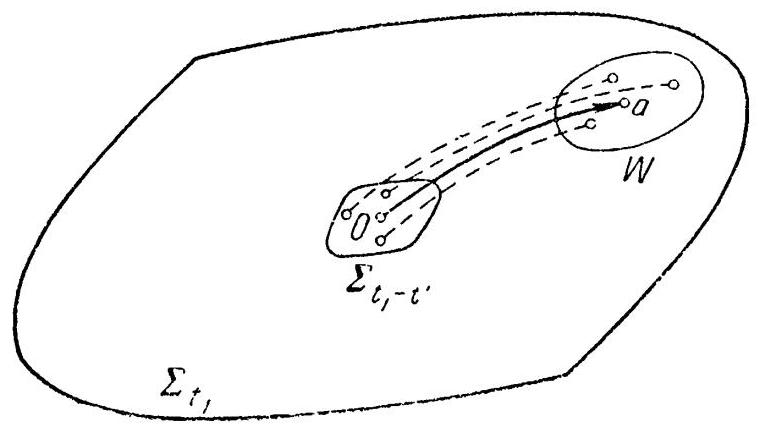
\includegraphics[max width=0.7\textwidth]{images/bo_d547imjef24c73bgfcdg_253_396_497_759_428_0.jpg}
\end{center}
\hspace*{3em}

Puc. 87.

Вернемся снова к оптимальным управлениям \(u\left( t\right),v\left( t\right)\) и оптимальным траекториям \(x\left( t\right),y\left( t\right)\), употинаемым в тео- реме 21 (при упрощающих предположениях (77)), и пока- жем,что точка \(x\left( T\right)\) лежит н а г р а н и ц е тела \({\sum }_{T}\). B ca- мом деле, допустим, что точка \(x\left( T\right)\) является внутренней точкой этого тела. Тогда в эту точку можно попасть (дви- гаясь от начала координат в силу системы (74)) за время \({t}^{\prime } < T\). Следовательно, взяв точку и удовлетворяющую неравенствам \({t}^{\prime } < {t}_{1} < T\),мы найдем,что множество \({\sum }_{{t}_{1}}\) (состоящее из точек, в которые можно попасть за время ну содержит точку х (т) внутри себя, а следовательно, со- держит внутри себя шар некоторого радиуса r с центром в точке \(x\left( T\right)\). При \({t}_{1} < t < T\) множество \({\sum }_{t}\) также содер- жит внутри себя map радиуса r с центром в точке x(T). Выберем теперь число t (принадлежащее интервалу \({t}_{1} < t < T)\) настолько близким к T, чтобы расстояние между точками \(y\left( T\right)  = x\left( T\right)\) и \(y\left( t\right)\) было меньше,чем r. Тогда множество \({\sum }_{t}\) содержит внутри себя точку \(y\left( t\right)\), причем \(t < T\). Ho это означает, что в положение \(y\left( t\right)\) преследующая точка может попасть в момент t/c T, т. е. что (при выбранном управлении \(v\left( t\right)\) для преследуемой точки) встреча может произойти в момент \(t < T\). Однако это противоречит определению числа Т. Таким образом, точка \(x\left( T\right)\) лежит на границе \({S}_{T}\) множества \({\sum }_{T}\).

Из этого следует, что \(u\left( t\right),0 \leq  t \leq  T\), есть оптималь- ное по быстродействию управление, соответствующее пере- ходу из начала координат в точку х (т) (в силу систе- мы (74)). Действительно, если бы это управление было не оптимальным, то в точку х (7) можно было бы попасть за время, меньшее чем T, и тогда точка х(T) лежала бы в н у т р и множества Σ т, что не имеет места. В силу ска- занного, управление \(u\left( t\right)\), рассматриваемое на отрезке \(0 \leq  t \leq  {t}_{1}\) (где \({t}_{1} < T\) ),также является оптимальным по быстродействию управлением, соответствующим переходу (в силу системы (74)) из начала координат в точку x(t,). Иначе говоря, в точку х(н) (О < с ; е т) нельзя попасть быстрее,чем за время \({t}_{1}\),и потому точка \(x\left( {t}_{1}\right)\) лежит на гра- нице множества \({\sum }_{{t}_{1}}\).

Обозначим через Σ объединение всех множеств Σ, \(t > 0\). Ясно, что Σ — открытое множество пространства Х, содержащее множество Х т и, следовательно, точку \(x\left( T\right)  = y\left( T\right)\). Поэтому найдется такое число t* < T, что \(y\left( t\right)  \in  \sum\) при \({t}^{ * } \leq  t \leq  T\). Для любого \(t,{t}^{ * } \leq  t \leq  T\),мы обо- значим через т(t) такое число, что у (t) ∈ \({S}_{\tau \left( t\right) }\). Легко видеть, что \(\tau \left( t\right)\) - непрерывная функция переменного \(t\), \({t}^{ * } \leq  t \leq  T\). Далее,так как \(u\left( t\right),v\left( t\right)\) - о п т и м а л ь н а я пара управлений и \(T\) - время преследования, то имеют место соотношения

\[
\tau \left( T\right)  = T, \tag{78}
\]

\[
\tau \left( t\right)  > t\text{ при }t < T\text{ . } \tag{79}
\]

В самом деле, если бы для некоторого \(t < T\) было вы- полнено неравенство \(\tau \left( t\right)  \leq  t\), то в точку \(y\left( t\right)  \in  {S}_{\tau \left( t\right) } \subset  {\sum }_{t}\) преследующая точка могла бы попасть в момент времени \(t\), т. е. (при выбранном управлении v(t) для преследуемой точки) была бы возможна встреча в момент \(t < T\),что противоречит определению числа Т.

Так как точка \(y\left( t\right)\) лежит на границе \({S}_{\tau \left( t\right) }\) выпуклого тела \({\sum }_{\tau \left( t\right) }\), to можно провести в X опорную гиперплоскость к телу Σ тен, проходящую через точку у (t). Эту гипер- плоскость (любую из них, если она не единственна) мы обозначим через \({\Delta }_{\tau \left( t\right) }\). Единичный вектор, ортогональный кгиперплоскости \({\Delta }_{\tau \left( t\right) }\) иидущий източки \(y\left( t\right)\) втополупро- странство, которое не содержит множества Хт(н), мы обозна- чим через в тит так как для любой точки \(x \in  {\sum }_{\tau \left( t\right) }\) вектор \(x - y\left( t\right)\) направлен в то полупространство, которое содер- жит множество \({\sum }_{\tau \left( l\right) }\), to \(\left( {x - y\left( t\right),{e}_{\tau \left( t\right) }}\right)  \leq  0\) (npu \(x \in  {\sum }_{\tau \left( t\right) }\) ). B частности, из (79) следует, что \({\sum }_{t} \subset  {\sum }_{\tau \left( t\right) }\), и потому

\[
\left( {x - y\left( t\right) ,{e}_{\tau \left( t\right) }}\right)  \leq  0\text{ при }x \in  {\sum }_{t}. \tag{80}
\]

Выберем теперь некоторый способ варьирования управ- ления \(v\left( t\right)\) (см. стр. 97—98). Соответствующая варьирован- ная траектория (с прежним начальным условием, см. (59)) имеет вид:

\[
{y}^{ * }\left( t\right)  = y\left( t\right)  + {\varepsilon \delta y}\left( t\right)  + o\left( \varepsilon \right) ,\;0 \leq  t \leq  T; \tag{81}
\]

при этом вектор \({\Delta y} = {\delta y}\left( T\right)\) определяется формулой (22), гл. 2, в которой следует положить \(\tau  = T,{\delta t} = 0\) и от- бросить координату х0 (πбо рассматривается фазовое про- странство \(X\), a не \(X\) ). \(\Pi\) усть теперь \({\varepsilon }_{1},{\varepsilon }_{2},\ldots,{\varepsilon }_{i},\ldots\) - произвольная сходящаяся к нулю последовательность положительных чисел. Траекторию (81), соответствующую значению \(\varepsilon  = {\varepsilon }_{i}\), обозначим через \({y}_{i}^{ * }\left( t\right)\), a соответствующее управление — через у ку не в не и не и не и не и еде я не не не не ветствующее управлению \({v}_{i}^{ * }\left( t\right)\),мы обозначим через \({t}_{i}\) : \({t}_{i} = {T}_{{v}_{i}^{ * }}\). Таким образом,

\[
{y}_{i}^{ * }\left( {t}_{i}\right)  \in  \mathop{\sum }\limits_{{t}_{i}},\;i = 1,2,\ldots \tag{82}
\]

Из оптимальности пары управлений и(t), v(t) вытекает, что

\[
{t}_{i} \leq  T,\;i = 1,2,\ldots \tag{83}
\]

Далее, легко видеть, что

\[
\mathop{\lim }\limits_{{i \rightarrow  \infty }}{t}_{i} = T \tag{84}
\]

В самом деле, допустим, что соотношение (84) не вы- полнено. Переходя, если нужно, к подпоследовательно- сти, мы можем считать, что lim н с уществует и < \(T\). Положим \(\mathop{\lim }\limits_{{i \rightarrow  \infty }}{t}_{i} = \widetilde{t}\). Так как ілім 83 е 30,103(81) следует, ЧТО

\[
\mathop{\lim }\limits_{{i \rightarrow  \infty }}{y}_{i}^{ * }\left( {t}_{i}\right)  = y\left( \widetilde{t}\right)
\]

Далее, из (82), переходя к пределу, получаем

\[
\mathop{\lim }\limits_{{i \rightarrow  \infty }}{y}_{i}^{ * }\left( {t}_{i}\right)  \in  {\sum }_{\widetilde{t}}
\]

Takum образом, \(y\left( \widetilde{t}\right)  \in  {\sum }_{\widetilde{t}}\),где \(\widetilde{t} < T\),но это противоречит определению Т. Следовательно, соотношение (84) выполнено.

Из (83) и (84) следует, что при достаточно большом \(i\) определены числа \(\tau \left( {t}_{i}\right)\) ; мы будем считать (отбрасывая, если нужно, несколько первых членов последовательности), что числа \(\tau \left( {t}_{i}\right)\) определены для всех i = 1,2,… Далее, из (78) и (84), в сплу непрерывности функции \(\tau \left( t\right)\), следует

\[
\mathop{\lim }\limits_{{i \rightarrow  \infty }}\tau \left( {t}_{i}\right)  = T \tag{85}
\]

Рассмотрим теперь векторы

\[
{e}_{\tau \left( {t}_{i}\right) },\;i = 1,2,\ldots \tag{86}
\]

В силу компактности единичной сферы n-мерного прост- ранства X, мы можем считать (перейдя, если нужно, к подпоследовательности), что векторы (86) сходятся при \(i \rightarrow  \infty\) к некоторому единичному вектору е пространства Х. Пусть теперь х — произвольная в н у т р е н н я я точка тела \({\sum }_{T}\). Тогда при достаточно большом i будет выполнено включение \(x \in  {\sum }_{{t}_{i}}\) и потому

\[
\left( {x - y\left( {t}_{i}\right) ,{e}_{\tau \left( {t}_{i}\right) }}\right)  \leq  0
\]

(см. (80)). Переходя в этом соотношении к пределу при \(i \rightarrow  \infty\),мы получим (учитывая соотношение у \(y\left( T\right)  = x\left( T\right)\) и соотношение (85)):

\[
\left( {x - x\left( T\right) ,e}\right)  \leq  0. \tag{87}
\]

Соотношение (87) справедливо для всех внутренних точек х тела \({\sum }_{T}\), a значит,и для всех вообще точек х этого тела.

Далее, из (82) следует, в силу (80), что

\[
\left( {{y}_{i}^{ * }\left( {t}_{i}\right)  - y\left( {t}_{i}\right) ,{e}_{\tau \left( {t}_{i}\right) }}\right)  \leq  0,\;i = 1,2,\ldots
\]

или, согласно (81),

\[
\left( {{\varepsilon }_{i}{\delta y}\left( {t}_{i}\right)  + o\left( \varepsilon \right) { \mid  }_{\varepsilon  = {\varepsilon }_{i}},{e}_{\tau \left( {t}_{i}\right) }}\right)  \leq  0,\imath  = 1,2,\ldots
\]

Разделив это соотношение на в и переходя к пределу

9 JI. C. Понтрягин и др. при \(i \rightarrow  \infty\),получим (в силу соотношения ihm \(\frac{o\left( \mathrm{e}\right) }{\varepsilon  \rightarrow  \infty } = 0\) )

\[
\left( {{\delta y}\left( T\right) ,e}\right)  \leq  0,
\]

или, иначе,

\[
\left( {{\Delta y},e}\right)  \leq  0. \tag{88}
\]

Наконец, рассмотрим функцию

\[
{\varphi }_{i}\left( t\right)  = \left( {x\left( t\right)  - y\left( t\right) ,{e}_{\tau \left( {t}_{i}\right) }}\right) .
\]

Так как \(x\left( t\right)  \in  \mathop{\sum }\limits_{t}\) при любом \(t\),то дз (80) следует,что \({\varphi }_{i}\left( {t}_{i}\right)  \leq  0\). Далее, \({\varphi }_{i}\left( T\right)  = 0\), nóo \(x\left( T\right)  = y\left( T\right)\). Kpome того, функция \({\varphi }_{i}\left( t\right)\) имеет при достаточно большом i непрерыв- ную производную на отрезке \({t}_{i} \leq  t \leq  T\) (ибо управления \(u\left( t\right)\) и \(v\left( t\right)\) кусочно-непрерывны и имеет место соотноше- ние (84)). Поэтому существует такое число \({\xi }_{i},{t}_{i} < {\xi }_{i} < T\), 470 \({\varphi }_{i}^{\prime }\left( {\xi }_{i}\right)  \geq  0\), r.e.

\[
\left( {f\left( {x\left( {\xi }_{i}\right) ,u\left( {\xi }_{i}\right) }\right)  - g\left( {y\left( {\xi }_{i}\right) ,v\left( {\xi }_{i}\right) ,{\xi }_{i}}\right) ,{e}_{\tau \left( {t}_{i}\right) }}\right)  \geq  0.
\]

Переходя в этом соотношении к пределу при \(i \rightarrow  \infty\), no- лучим

\[
\left( {w,e}\right)  \leq  0, \tag{89}
\]

где

\[
w = g\left( {y\left( T\right) ,v\left( T\right) ,T}\right)  - f\left( {x\left( T\right) ,u\left( T\right) }\right) . \tag{90}
\]

Обозначим теперь через ∆ гиперплоскость пространст- ва \(X\), проходящую через точку х(Т) и ортогональную вектору е. Кроме того, будем считать векторы Δ \(y\) и и исходящими из точки \(x\left( T\right)\). Тогда соотношения (87),(88) 11 (89) показывают, что все тело \({\sum }_{T}u\) векторы \({\Delta y}\;u\;w\) расположены по одну сторону гиперплоскости ∆. Иначе говоря, если мы обозначим через Σ* выпуклую оболочку тела \({\sum }_{T}\) и вектора w, то мы найдем, что тело Σ* и вектор \({\Delta y}\) лежат по одну сторону гиперплоскости Δ. Поэтому тело Σ* и вектор — Δy расположены в двух раз ны х замкнутых полупространствах, определяемых гиперпло- скостью Δ. Отсюда мы, наконец, заключаем, что вектор \(- {\Delta y},{ucxo}\partial x.{uu}\partial x\partial y.u\partial x\left( T\right)\),не проходит через вну- тренние точки тела Σ*.

Будем теперь рассматривать всевозможные способы варьирования управления v(t), откладывая получающиеся векторы \({\Delta y} = {\delta y}\left( T\right)\) (см. (81)) из точки \(x\left( T\right)\). Концы этих векторов заполнят некоторое множество К в пространстве \(X\),являющееся, как легко видеть (ср. стр. 105—106), выпук- лым конусом с вершиной в точке x(T). Концы векторов — Δ \(y\) заполняют выпуклый конус, симметричный конусу K относительно точки \(x\left( T\right)\). Этот конус мы обозначим через \(- K\). Из сказанного выше вытекает, что конус — \(K\) не пересекается с внутренностью выпуклого тела Σ*. Так как при этом тело Σ* содержит внутренние точки (ибо тело \({\sum }_{T}\) содержит внутренние точки), то тела Σ* и —К являются разделяемыми. Иначе говоря, существует в X такая гиперплоскость ∆*, что тело Σ* содержится в одном замкнутом полупространстве, определяемом гипер- плоскостью Δ*, а конус — \(K\) в другом. Следовательно, выпуклые множества Σ* и K расположены в одном замк- нутом полупространстве, определяемом гиперплоскостью Δ*. Обозначим через е* единичный вектор, исходящий из точки \(x\left( T\right)\), ортогональный гиперплоскости \(\Delta  *\) и направ- ленный в полупространство, не содержащее тел Σ* и K. Таким образом, вектор е* удовлетворяет соотнотениям (cp. \(\left( {87}\right),\left( {88}\right),\left( {89}\right) )\) :

\[
\left( {x - x\left( T\right) ,{e}^{ * }}\right)  \leq  0\text{ при }x \in  {\sum }_{T}, \tag{91}
\]

\[
\left( {{\Delta y},{e}^{ * }}\right)  \leq  0\text{ при }{\Delta y} \in  K, \tag{92}
\]

\[
\left( {w,{e}^{ * }}\right)  \leq  0\text{ . } \tag{93}
\]

Обозначим через ψ(t) решение системы (63) с началь- ным условием \(\psi \left( T\right)  = {e}^{ * }\), a через \(\chi \left( t\right)\) - решение системы (64) с начальным условием \(\chi \left( T\right)  = {e}^{ * }\). Мы покажем сей- час, что функции ψ(t) и χ(t) — искомые (т. е. они удо- влетворяют условиям, указанным в теореме 21). Прежде всего отметим, что в силу выбора начальных условий для функций ψ(t) и χ(t) соотношение (68) выполнено. Далее, из (90) и (93) непосредственно следует соотношение (67). На- конец, соотношения (65) и (66) доказываются, исходя из неравенств (91) и (92), совершенно так же, как в главе 2 из неравенства (34) было доказано соотношение (11) (в до- казательстве должны быть сделаны очевидные изменения, связанные с тем, что рассматривается пространство X, а не \(X\) ).

Итак, теорема 21 полностью доказана.

\section*{ПРИНЦИП МАКСИМУМА И ВАРИАЦИОННОЕ ИСЧИСЛЕНИЕ}

В этой главе мы рассмотрим связь, существующую между теорией оптимальных процессов и классическим вариационным исчислением. Будет показано, что оптималь- ная задача, изученная в главах 1, 2, является обобще- нием задачи Лагранжа в вариационном исчислении и эквивалентна ей в случае, когда область управления U является открытым множеством r-мерного векторного про- странства \({E}_{r}\).

Далее, мы покажем, что в случае о т к р ы т о г о мно- жества U из принципа максимума следуют все основные необходимые условия, известные в вариационном исчис- лении (в частности, критерий Вейерштрасса). Однако в случае, когда \(U - 3\) ам к н у т о е множество простран- ства \({E}_{r}\) (не совпадающее со всем \({E}_{r}\) ), условле Вейерштрасса перестает действовать, т. е. теорема о том, что для дости- жения минимума функционала необходимо выполнение условия Вейерштрасса, становится н е в е р н о й. Та- ким образом, существенное преимущество принципа макси- мума по сравнению с классическими теоремами вариацион- ного исчисления состоит в том, что он применим для любого (в частности, замкнутого) множества UCE, Ro Cumupe- ние класса возможных областей управления U по сравнению с классическим случаем открытых множеств весьма существенно для технических приложений теории. Именно случай 3 а м к н у т о г о множества UCE, най- более интересен в задачах оптимального управления и, в частности, в прикладных вопросах. Например, даже прос- тейшие задачи,приведенные в §5, не могли бы быть рас- смотрены методами классического вариационного исчисле- ния, так как область управления U являлась замкнутым множеством и значения оптимальных управлений во всех примерах лежали н а гран и ц е И. Если в любом из этих примеров мы ограничимся рассмотрением открытого множества, отбросив граничные точки области управления \(U\), то классические теоремы дадут такой ответ: оптималь- ных управлений не существует. Это, конечно, может служить указанием на то, что управляющий параметр дол- жен принимать значения н а r p a h и ц e множества U, но такого соображения отнюдь не достаточно для решения задачи, ибо нужно знать, каким обр а з ом должен изменяться управляющий параметр на границе области U. Например, в случае линейных задач нужно знать, каково может быть число переключений, из каких вершин много- гранника U в какие происходят переключения и т. п. На эти вопросы классическая теория на может дать никакого ответа; в то же время, как мы видели на примерах, прин- цип максимума содержит информацию, достаточную для решения указанных вопросов.

В § 29 мы выведем из принципа максимума необхо- димые условия для основной задачи вариационного исчис- ления.

B § 30 мы докажем эквивалентность задачи JIa- гранжа и оптимальной задачи гл. 2, а также выведем из принципа максимума критерий Вейерштрасса в случае, когда область управления Й представляет собой откры- тое множество r-мерного векторного пространства E,. Для простоты изложения мы ограничимся рассмотрением силь- ных экстремумов вариационных задач.

\section*{§ 29. Основная задача вариационного исчисления}

Хотя основная задача вариационного исчисления и является частным случаем задачи Лагранжа, рассматри- ваемой в следующем параграфе, тем не менее мы посвя- щаем основной задаче отдельный параграф, так как связь между принципом максимума и необходимыми условиями вариационного исчисления особенно отчетливо выступает в этом простейшем случае.

\section*{Определения}

Пусть в (n + 1)-мерном пространстве R\textasciicircum +1 действитель- ных переменных \(\left( {t,{x}^{1},\ldots,{x}^{n}}\right)  = \left( {t,x}\right)\) задана кривая \(x\left( t\right)\) уравнениями

\[
{x}^{i} = {x}^{i}\left( t\right) ,\;i = 1,\ldots ,n,{t}_{0} \leq  t \leq  {t}_{1}. \tag{1}
\]

Если функции \({x}^{i}\left( t\right),i = 1,\ldots,n\), абсолютно непрерывны и имеют ограниченные производные, т. е. во всякой точке существования производной выполнено соотношение

\[
\left| \frac{d{x}^{i}\left( t\right) }{dt}\right|  \leq  M = \text{ const },\;i = 1,\ldots ,n,
\]

то мы будем говорить, что кривая (1) абсолютно непре- рывна. Далее, обозначим точки \(x\left( {t}_{0}\right)\) и \(x\left( {t}_{1}\right)\) соответствен- но через х, и и и и и и и из и я и поривить, что кривая (1) соеди- няет точки (и, ио) и (и, и, или же что она удовлетворяет краевым условиям

\[
x\left( {t}_{0}\right)  = {x}_{0},\;x\left( {t}_{1}\right)  = {x}_{1}. \tag{2}
\]

Назовем δ-окрестностью абсолютно непрерывной кривой (1) множество всех абсолютно непрерывных кривых

\[
\widetilde{x}\left( t\right)  = \left( {{\widetilde{x}}^{1}\left( t\right) ,\ldots ,{\widetilde{x}}^{n}\left( t\right) }\right) ,\;{t}_{0} \leq  t \leq  {t}_{1},
\]

удовлетворяющих условию

\[
\left| {{x}^{i}\left( t\right)  - {\widetilde{x}}^{i}\left( t\right) }\right|  < \delta \text{ при }{t}_{0} \leq  t \leq  {t}_{1},\;i = 1,2,\ldots ,n.
\]

Пусть теперь G — некоторое открытое множество про- странства R** и пусть действительная функция

\[
f\left( {t,{x}^{1},\ldots ,{x}^{n},{u}^{1},\ldots ,{u}^{n}}\right)  = f\left( {t,x,u}\right)
\]

определена для любой точки (t, x)∈G и любых действи- тельных значений и’,..., иГ. Будем предполагать, кроме того, что функция \(f\) непрерывна и непрерывно дифферен- цируема по всем аргументам.

Предположим, что кривая (1) целиком лежит в области G. Тогда определен интеграл

\[
J = J\left( x\right)  = {\int }_{{t}_{0}}^{{t}_{1}}f\left( {t,x\left( t\right) ,\frac{{dx}\left( t\right) }{dt}}\right) {dt} \tag{3}
\]

который мы будем рассматривать как функционал от вектор-функции \(x\left( t\right)\), \({t}_{0} \leq  t \leq  {t}_{1}\). Очевидно, что для любой кривой \(\widetilde{x}\left( t\right),{t}_{0} \leq  t \leq  {t}_{1}\),принадлежащей б-окрест- ности кривой (1), функционал \(J\left( \widetilde{x}\right)\) также определен, если \(\delta  > 0\) достаточно мало.

Абсолютно непрерывную кривую (1) назовем (сильной) экстремалью для функционала (3), если существует такое \(\delta  > 0\),что на множестве всех кривых \(\widetilde{x}\left( t\right),{t}_{0} \leq  t \leq  {t}_{1}\), расположенных в δ-окрестности кривой (1) и удовле- творяющих тем же краевым условиям (2), функционал (3) принимает свое наименьшее (или наибольшее) значение при \(\widetilde{x} = x\). В дальнейшем мы будем рассматривать только случай м и н и м у м а. Таким образом, кривая (1) будет называться экстремалью функционала (3), если существует такое б > 0, что для любой абсолютно непрерывной кривой \(\widetilde{x}\left( t\right),{t}_{0} \leq  t \leq  {t}_{1}\),принадлежащей б-окрестности кривой (1) и удовлетворяющей краевым условиям X(t,0) = х, т. (i) = (1, выполнено неравенство \(J\left( \widetilde{x}\right)  \geq  J\left( x\right)\).

Основная задача вариационного исчисления состоит в нахождении всех экстремалей данного функционала (3) при заданных (закрепленных) краевых условиях (2). Уравнения Эйлера и условие Лежандра

Мы покажем сейчас, что всякая экстремаль является оптимальной траекторией для некоторой оптимальной за- дачи. Рассмотрим следующую систему n-ro порядка:

\[
\frac{d{x}^{i}}{dt} = {u}^{i},\;i = 1,\ldots ,n, \tag{4}
\]

и интегральный функционал

\[
J = J\left( {x,u}\right)  = {\int }_{{t}_{0}}^{{t}_{1}}f\left( {t,{x}^{1},\ldots ,{x}^{n},{u}^{1},\ldots ,{u}^{n}}\right) {dt} =
\]

\[
= {\int }_{{t}_{0}}^{{t}_{1}}f\left( {t,x,u}\right) {dt}. \tag{5}
\]

Здесь \(u = \left( {{u}^{1},\ldots,{u}^{n}}\right)\) - управляющий параметр,который выбирается в классе всех ограниченных измеримых век- тор-функций. Таким образом, область управления U сов- падает в данном случае со всем n-мерным пространством \({E}_{n}\) переменных \({u}^{1},\ldots,{u}^{n}\).

Имея в виду применения к вариационному исчисле- нию, мы определим здесь оптимальные траектории задачи (4), (5) несколько иначе, чем это было сделано в главах 1, 2. Именно, пусть пределы интегрирования в (5) фик- сированы. Измеримое ограниченное управление и(t), \({t}_{0} \leq  t \leq  {t}_{1}\),и соответствующую абсолютно непрерывную траекторию \(x\left( t\right)\) системы (4) с краевыми условиями (2) мы будем называть оптимальными, если существует такое \(\delta  > 0\),что,каково бы ни было управление и(t),для кото- poro соответствующая траектория \(\widetilde{x}\left( t\right)\) системы (4) удов- летворяет краевым условиям (2) и находится в 6-окрест- ности кривой х(t), выполняется неравенство J(x, u) \(\geq \; \geq  J\left( {x,u}\right)\). Иначе говоря, здесь при определении оптималь- ных управлений и траекторий мы будем сравнивать траек- торию \(x\left( t\right)\) не с о в с е м и другими траекториями \(\widetilde{x}\left( t\right)\), а только с траекториями, расположенными в δ-окрестности кривой \(x\left( t\right)\). Всякая траектория, оптимальная в смысле гл. 1, 2, является оптимальной и в смысле принятого здесь определения, но, вообще говоря, не наоборот. Таким обра- зом, оптимальных управлений и траекторий в принятом здесь смысле б о л ь ш е, чем оптимальных управлений и траекторий в смысле глав 1, 2.

Нетрудно понять, однако, что принцип максимума, как н е о б х о д и м о е условие оптимальности, для оптималь- ных управлений и траекторий в принятом здесь смысле сохраняется в той же самой формулировке. В самом деле, при доказательстве принципа максимума в главе 2 мы сравнивали траекторию \(x\left( t\right)\) только с траекториями вида

\[
{x}^{ * }\left( t\right)  = x\left( t\right)  + {\varepsilon \delta x}\left( t\right)  + o\left( \varepsilon \right) ,
\]

где ε — бесконечно малая величина. При достаточно малом в траектория \({x}^{ * }\left( t\right)\) лежит в δ-окрестности кривой \(x\left( t\right)\) (ка- ково бы ни было заданное число б), и поэтому все рас- суждения главы 2 проходят б е з и з м е н е н и й для управлений и траекторий, оптимальных в рассматриваемом здесь смысле.

Сформулированная оптимальная задача (4), (5) являет- ся задачей с закрепленными концами и закрепленным временем (см. § 8). Очевидно, что всякая оптимальная тра- ектория задачи (4), (5) является экстремалью интеграла (3) и наоборот (достаточно, в силу (4), заменить в интег- рале (5) величины \({u}^{i}\left( t\right)\) производными \(\frac{d{x}^{i}\left( t\right) }{dt}\) ). Поэтому принцип максимума, представляющий собой необходимое условие оптимальности, является в то же время и необхо- димым условием для того, чтобы кривая \(x\left( t\right)\) была экстре- малью интеграла (3). Это простое соображение и позво- ляет применять принцип максимума при решении вари- ационной задачи (3).

В силу теоремы 6 для решения поставленной оптималь- ной задачи мы должны составить уравнения для вспомо- гательных неизвестных цо, \({\psi }_{1},\ldots,{\psi }_{n}\) и функцию \(\mathcal{H}\), которые, в силу (4), принимают здесь вид

\[
\mathcal{K} = {\psi }_{0}f\left( {t,x,u}\right)  + {\psi }_{1}{u}^{1} + {\psi }_{2}{u}^{2} + \ldots  + {\psi }_{n}{u}^{n}, \tag{6}
\]

\[
\left. \begin{array}{l} \frac{d{\psi }_{0}}{dt} = 0, \\  \frac{d{\psi }_{i}}{dt} =  - {\psi }_{0}\frac{\partial f\left( {t,x,u}\right) }{\partial {x}^{i}},i = 1,\ldots ,n. \end{array}\right\} \tag{7}
\]

Условие максимума, указанное в теореме 6, дает

\[
\mathcal{K}\left( {\psi \left( t\right) ,x\left( t\right) ,t,u\left( t\right) }\right)  =
\]

\[
= \mathop{\max }\limits_{{u \in  {E}_{n}}}\left( {{\psi }_{0}f\left( {t,x\left( t\right) ,u}\right)  + \mathop{\sum }\limits_{{\alpha  = 1}}^{n}{\psi }_{\alpha }\left( t\right) {u}^{\alpha }}\right) \tag{8}
\]

(почти всюду на отрезке б, с < 6 с, ср. теорему 8). Так как область управления \(U\) совпадает со всем простран- ством Е „ (для справедливости последующих рассужде- ний достаточно было бы потребовать, чтобы она была о т к р ы т ы м множеством в Е„), то точка максимума \(u = u\left( t\right)\) функции \(\mathcal{K}\left( {\psi \left( t\right),x\left( t\right),t,u}\right)\), рассматриваемой как функция переменного и с/с, является ее с т а ц и о - на р н о й точкой. Следовательно, из (8) вытекает, что

(почти для всех t, \({t}_{0} \leq  t \leq  {t}_{1}\) ) выполнены соотношения:

\[
\frac{\partial }{\partial {u}^{l}}\mathcal{K}\left( {\psi \left( t\right) ,x\left( t\right) ,t,u\left( t\right) }\right)  = {\psi }_{0}\frac{\partial f\left( {t,x\left( t\right) ,u\left( t\right) }\right) }{\partial {u}^{l}} + {\psi }_{i}\left( t\right)  = 0,
\]

\[
i = 1,2,\ldots ,n.
\]

Из этих равенств следует, что цо ≠ 0, так как в против- ном случае мы имели бы \({\psi }_{i}\left( t\right)  \equiv  0,i = 0,1,\ldots,n\). Сле- довательно, мы можем считать, что цо — —1, так как \({\psi }_{0} =\) const \(\leq  0\left( {\mathrm{{cm}}\text{. теорему 6), a величины }{\psi }_{0},{\psi }_{1},\ldots }\right)\)..., \({\psi }_{n}\) определены лишь с точностью до общего положи- тельного множителя пропорциональности. Полагая в пре- дыдущих равенствах \({\psi }_{0} =  - 1,\) мы получаем (почти всюду на отрезке \({t}_{0} \leq  t \leq  {t}_{1}\) )

\[
{\psi }_{i}\left( t\right)  = \frac{\partial f\left( {t,x\left( t\right) ,u\left( t\right) }\right) }{\partial {u}^{i}},\;i = 1,\ldots ,n. \tag{9}
\]

C другой стороны, подставляя в уравнения (7) \({\psi }_{0} =  - 1\) и интегрируя, мы находим

\[
{\psi }_{i}\left( t\right)  = {\psi }_{i}\left( {t}_{0}\right)  + {\int }_{{t}_{0}}^{t}\frac{\partial f\left( {\tau ,x\left( \tau \right) ,u\left( \tau \right) }\right) }{\partial {x}^{i}}{d\tau }
\]

\[
i = 1,\ldots ,n,\;{t}_{0} \leq  t \leq  {t}_{1} \tag{10}
\]

Из (9) и (10) мы получаем уравнения Эйлера в интег- ральной форме (подставив вместо \({u}^{i}\left( t\right)\) производные д (см. (4)):

\[
\frac{\partial f\left( {t,x\left( t\right) ,\frac{{dx}\left( t\right) }{dt}}\right) }{\partial {u}^{i}}\left(  = \right) {\int }_{{t}_{0}}^{t}\frac{\partial f\left( {\tau ,x\left( \tau \right) ,\frac{{dx}\left( \tau \right) }{dt}}\right) }{\partial {x}^{i}}{d\tau } + {\psi }_{i}\left( {t}_{0}\right) ,
\]

\[
i = 1,\ldots ,n,
\]

где символ (=) означает, как и в главе 2, что равен- ства выполняются почти для всех t, \({t}_{0} \leq  t \leq  {t}_{1}\). Диффе- ренцирование по \(t\) (при условии, что функция \(f\) и экстре- маль х (t) дважды непрерывно дифференцируемы) дае уравнения Эйлера в обычном виде

\[
\frac{\partial f\left( {t,x\left( t\right) ,\frac{{dx}\left( t\right) }{dt}}\right) }{\partial {x}^{i}} - \frac{d}{dt}\left( \frac{\partial f\left( {t,x\left( t\right) ,\frac{{dx}\left( t\right) }{dt}}\right) }{\partial {u}^{i}}\right) \left(  = \right) 0, \tag{10}
\]

\[
i = 1,\ldots ,n\text{ . }
\]

Предположим теперь, что функция \(f\left( {t,x,u}\right)\) имеет в т о р ы е непрерывные частные производные по перемен- ным \({u}^{1},\ldots,{u}^{n}\). Тогда, если функция

\[
\mathcal{K}\left( {\psi \left( t\right) ,x\left( t\right) ,t,u}\right)  = f\left( {t,x\left( t\right) ,u}\right)  + \mathop{\sum }\limits_{{\alpha  = 1}}^{n}{\psi }_{\alpha }\left( t\right) {u}^{\alpha },
\]

как функция переменного \(u\),достигает в точке \(u = {u}_{0}\) максимума, то квадратичная форма

\[
\mathop{\sum }\limits_{{\alpha ,\beta  = 1}}^{n}\frac{{\partial }^{2}}{\partial {u}^{\alpha }\partial {u}^{\beta }}\mathcal{K}\left( {\psi \left( t\right) ,x\left( t\right) ,t,{u}_{0}}\right) {\xi }^{\alpha }{\xi }^{\beta } =
\]

\[
=  - \mathop{\sum }\limits_{{\alpha ,\beta  = 1}}^{n}\frac{{\partial }^{2}}{\partial {u}^{\alpha }\partial {u}^{\beta }}f\left( {t,x\left( t\right) ,{u}_{0}}\right) {\xi }^{\alpha }{\xi }^{\beta }
\]

неположительна (при любых б',..., ξ \({}^{n}\) ). Следовательно, из условия максимума (8) вытекает, что почти для всех t, \({t}_{0} \leq  t \leq  {t}_{1}\),выполняется неравенство

\[
\mathop{\sum }\limits_{{\alpha ,\beta  = 1}}^{n}\frac{{\partial }^{2}f\left( {t,x\left( t\right) ,\frac{{dx}\left( t\right) }{dt}}\right) }{\partial {u}^{\alpha }\partial {u}^{\beta }}{\xi }^{\alpha }{\xi }^{\beta } \geq  0.
\]

Это условие, необходимое для того, чтобы кривая \(x\left( t\right)\) была экстремалью интеграла (3), называется условием Лежандра.

\section*{Канонические переменные}

Пусть, как и выше, \(u\left( t\right),x\left( t\right),{t}_{0} \leq  t \leq  {t}_{1}\),— оптималь- ное управление и оптимальная траектория задачи (4), (5), a \(\psi \left( t\right)  = \left( {-1,{\psi }_{1}\left( t\right),\ldots,{\psi }_{n}\left( t\right) }\right)  = \left( {-1,\psi \left( t\right) }\right)\) - coor- ветствующее им ненулевое абсолютно непрерывное реше- ние системы (7).

Обозначим через \(\mathcal{M}\left( {\psi,x,t}\right)\) точную верхнюю грань значений функции \(\mathcal{K}\left( {\psi,x,t,u}\right)\) при фиксированных \(\psi  = \left( {-1,\psi }\right),x,t :\)

\(\mathcal{M}\left( {\psi ,x,t}\right)  = \mathop{\sup }\limits_{{u \in  {E}_{n}}}\mathcal{K}\left( {\psi ,x,t,u}\right)  =\)

\[
= \mathop{\sup }\limits_{{u \in  {E}_{n}}}\left( {-f\left( {t,x,u}\right)  + \mathop{\sum }\limits_{{\alpha  = 1}}^{n}{\psi }_{\alpha }{u}^{\alpha }}\right) .
\]

Предположим, что уравнение

\[
\mathcal{K}\left( {\psi ,x,t,u}\right)  = \mathcal{M}\left( {\psi ,x,t}\right) \tag{11}
\]

имеет единственное решение

\[
u = u\left( {\psi ,x,t}\right) , \tag{12}
\]

определенное, непрерывное и непрерывно дифференцируе- мое по своим аргументам при

\[
{t}_{0} \leq  t \leq  {t}_{1},\left| {{x}^{i} - {x}^{i}\left( t\right) }\right|  < \delta ,\left| {{\psi }_{i} - {\psi }_{i}\left( t\right) }\right|  < \delta , \tag{13}
\]

\[
i = 1,\ldots ,n,
\]

где б — достаточно малое положительное число. При этих условиях переменные \(\left( {{x}^{1},\ldots,{x}^{n}}\right)  = x,\left( {{\psi }_{1},\ldots,{\psi }_{n}}\right)  = \psi\) назовем каноническими переменными рассматриваемой оптимальной задачи, а функцию

\[
H\left( {\psi ,x,t}\right)  =  - f\left( {t,x,u\left( {\psi ,x,t}\right) }\right)  + \mathop{\sum }\limits_{{a = 1}}^{n}{\psi }_{a}{u}^{a}\left( {\psi ,x,t}\right)
\]

— функцией Гамильтона.

Так как оптимальное управление и (t) почти всюду на отрезке бо ≤ t ≤ t, удовлетворяет условию максимума (8) (напомним, что \({\psi }_{0} =  - 1\) ) и так как \(u\left( {\psi,x,t}\right)\) - ед и я с т в е н н о е решение уравнения (11) (при усло- виях (13)), то (почти всюду на отрезке б, еже (14)

\[
u\left( t\right)  = u\left( {\psi \left( t\right) ,x\left( t\right) ,t}\right)  = \frac{{dx}\left( t\right) }{dt}. \tag{14}
\]

Можно даже утверждать, что равенство (14) выполняется в с юд у на отрезке \({t}_{0} \leq  t \leq  {t}_{1}\). В самом деле, так как равенство (14) выполняется почти всюду, то

\[
x\left( t\right)  = x\left( {t}_{0}\right)  + {\int }_{{t}_{0}}^{t}u\left( {\psi \left( \tau \right) ,x\left( \tau \right) ,\tau }\right) {d\tau }.
\]

Но подынтегральная функция н е п р е р ы в н а по т (ибо решение (12) непрерывно по совокупности своих аргумен- тов), и потому в к а ж д о й точке отрезка бо ≤ ± ≤ t производная интеграла равна подынтегральной функ- ции.

Из равенства (11) следует, что частные производ- ные функции \(\mathcal{K}\left( {\psi,x,t,u}\right)\) no \({u}^{i},i = 1,\ldots,n\), обра- щаются в нуль при \(u = u\left( {\psi,x,t}\right)\) (если выполнены усло- вия (13)):

\[
- \frac{\partial f\left( {t,x,u\left( {\psi ,x,t}\right) }\right) }{\partial {u}^{i}} + {\psi }_{i} = 0,\;i = 1,\ldots ,n. \tag{15}
\]

Следовательно,

\[
\frac{\partial H\left( {\psi ,x,t}\right) }{\partial {\psi }_{i}} =
\]

\[
=  - \mathop{\sum }\limits_{{\alpha  = 1}}^{n}\frac{\partial f}{\partial {u}^{\alpha }} \cdot  \frac{\partial {u}^{\alpha }\left( {\psi ,x,t}\right) }{\partial {\psi }_{i}} + {u}^{i}\left( {\psi ,x,t}\right)  + \mathop{\sum }\limits_{{\alpha  = 1}}^{n}{\psi }_{\alpha }\frac{\partial {u}^{\alpha }\left( {\psi ,x,t}\right) }{\partial {\psi }_{i}} =
\]

\[
= {u}^{i}\left( {\psi ,x,t}\right)  + \mathop{\sum }\limits_{{\alpha  = 1}}^{n}\left( {{\psi }_{\alpha } - \frac{\partial f}{\partial {u}^{\alpha }}}\right) \frac{\partial {u}^{\alpha }}{\partial {\psi }_{i}} = {u}^{i}\left( {\psi ,x,t}\right) ;
\]

\[
\frac{\partial H\left( {\psi ,x,t}\right) }{\partial {x}^{i}} =
\]

\[
=  - \frac{\partial f}{\partial {x}^{i}} - \mathop{\sum }\limits_{{\alpha  = 1}}^{n}\frac{\partial f}{\partial {u}^{\alpha }} \cdot  \frac{\partial {u}^{\alpha }\left( {\psi ,x,t}\right) }{\partial {x}^{i}} + \mathop{\sum }\limits_{{\alpha  = 1}}^{n}{\psi }_{\alpha }\frac{\partial {u}^{\alpha }\left( {\psi ,x,t}\right) }{\partial {x}^{i}} =
\]

\[
=  - \frac{\partial f}{\partial {x}^{i}} + \mathop{\sum }\limits_{{\alpha  = 1}}^{n}\left( {{\psi }_{\alpha } - \frac{\partial f}{\partial {u}^{\alpha }}}\right) \frac{\partial {u}^{\alpha }}{\partial {x}^{i}} =  - \frac{\partial f\left( {t,x,u\left( {\psi ,x,t}\right) }\right) }{\partial {x}^{i}}.
\]

Полученные соотношения, в силу (14), (7), приводят нас

к каноническим уравнениям Эйлера — Гамильтона:

\[
\frac{d{x}^{i}}{dt} = \frac{\partial H}{\partial {\psi }_{i}},\;i = 1,\ldots ,n,
\]

\[
\frac{d{\psi }_{i}}{dt} =  - \frac{\partial H}{\partial {x}^{i}},i = 1,\ldots ,n,
\]

которым удовлетворяют в каждой точке отрезка бо ≤ t ≤ t, координаты вектор-функций \(x\left( t\right)  = \left( {{x}^{1}\left( t\right),\ldots,{x}^{n}\left( t\right) }\right)\) и \(\psi \left( t\right)  = \left( {{\psi }_{1}\left( t\right),\ldots,{\psi }_{n}\left( t\right) }\right).\)

Предположим, наконец, функцию f(t, x, u) д в а ж д ы непрерывно дифференцируемой по переменным \({u}^{1},\ldots,{u}^{n}\) и пусть определитель

\[
\left| {\frac{{\partial }^{2}}{\partial {u}^{i}\partial {u}^{J}}f\left( {t,x\left( t\right) ,u\left( {\psi \left( t\right) ,x\left( t\right) ,t}\right) }\right) }\right| \tag{16}
\]

отличен от нуля при бо ≤ t < t, В этом случае система уравнений

\[
{\psi }_{i} - \frac{\partial f\left( {t,x,u}\right) }{\partial {u}^{i}} = 0,\;i = 1,\ldots ,n, \tag{17}
\]

однозначно разрешима относительно \({u}^{1},\ldots,{u}^{n}\), если \({x}^{i}\) и \({\psi }_{i}\) мало отличаются от \({x}^{i}\left( t\right)\) и н, в силу (15), решение этой системы совпадает с функцией (12). Таким образом, данное нами выше определение канонических координат согласуется с обычным определением этих координат с помощью системы (17) при условии, что определитель (16) не обращается в нуль.

Замечание. Если предположить, что функция \(f\left( {t,x,u}\right)\) определена не для всех вещественных значений переменных \({u}^{1},\ldots,{u}^{n}\), a только при \(u \in  U \subset  {E}_{n}\),где \(U -\) некоторое открытое множество в \({E}_{n}\), то (после очевидных изменений в определении экстремалей для интеграла (3)), все изложенное остается в силе. Надо только в соответ- ствующей оптимальной задаче (4), (5) в качестве области управления взять не все пространство \({E}_{n}\), a ero откры- тое подмножество И. Это замечание относится и к сле- дующему параграфу.

\section*{§ 30. Задача Лагранжа}

Формулировка задачи

Пусть заданы \(k\) функций

\[
{f}^{i}\left( {t,{x}^{1},\ldots ,{x}^{n},{v}^{1},\ldots ,{v}^{n - k}}\right)  = {f}^{i}\left( {t,x,v}\right) ,\;i = 1,\ldots ,k,
\]

непрерывных и непрерывно дифференцируемых по всем аргументам при (t, x)∈G и при любых значениях век- тора v = (v',..., v'), где r = n - k. Рассмотрим следую- щую систему к дифференциальных уравнений с п неизвестными функциями \({x}^{1}\left( t\right),\ldots,{x}^{n}\left( t\right)\) :

\[
\frac{d{x}^{i}}{dt} - {f}^{i}\left( {t,{x}^{1},\ldots ,{x}^{n},\frac{d{x}^{h + 1}}{dt},\ldots ,\frac{d{x}^{n}}{dt}}\right)  \equiv
\]

\[
\equiv  {\varphi }^{i}\left( {t,{x}^{1},\ldots ,{x}^{n},\frac{d{x}^{1}}{dt},\ldots ,\frac{d{x}^{n}}{dt}}\right)  = 0, \tag{18}
\]

\[
i = 1,\ldots ,k < n\text{ . }
\]

Абсолютно непрерывную кривую \(x\left( t\right)\), \({t}_{0} \leq  t \leq  {t}_{1}\), целиком лежащую в области G, будем называть допу- стимой, если она удовлетворяет краевым условиям (2), а ее координаты — системе (18). Далее, абсолютно непре- рывную кривую \(x\left( t\right),{t}_{0} \leq  t \leq  {t}_{1}\),мы будем называть экстремалью для функционала (3) при заданных краевых условиях (2) и заданной системе (18), если х (t) — допу- стимая кривая и существует такое ε±0, что J (x) ≤ \(\leq  J\left( \widetilde{x}\right)\) для любой до п у с т п мо й кривой \(\widetilde{x}\left( t\right)\), \({t}_{0} \leq  t \leq  {t}_{1}\),лежащей в 8-окрестности кривой \(x\left( t\right)\).

Задача Лагранжа (с закрепленными концами) при заданных краевых условиях (2) и заданной системе (18) заключается в нахождении всех экстремалей для функ- ционала вида (3).

Покажем, что эта задача сводится к некоторой опти- мальной задаче. Для симметрии введем обозначение

\[
{f}^{0}\left( {t,x,v}\right)  =
\]

\[
= f\left( {t,x,{f}^{1}\left( {t,x,v}\right) ,\ldots ,{f}^{h}\left( {t,x,v}\right) ,{v}^{1},\ldots ,{v}^{r}}\right) , \tag{19}
\]

где функция \(f\left( {t,x,{u}^{1},\ldots,{u}^{n}}\right)\) определена в предыдущем параграфе.

Рассмотрим систему n-го порядка

\[
\left. \begin{aligned} \frac{d{x}^{i}}{dt} &  = {f}^{i}\left( {t,x,v}\right) ,i = 1,\ldots ,k, \\  \frac{d{x}^{h + j}}{dt} &  = {v}^{j},j = 1,\ldots ,n - k = r, \end{aligned}\right\} \tag{20}
\]

в которой через \(v = \left( {{v}^{1},\ldots,{v}^{r}}\right)\) обозначен управляющий вектор. Допустимыми будем считать любые измеримые ограниченные управления, т. е. областью управления слу- жит все r-мерное пространство \({E}_{r}\) переменных \({v}^{1},\ldots,{v}^{r}\).

Требуется найти допустимое управление v (t), кото- рому соответствует траектория \(x\left( t\right)\) системы (20), удов- летворяющая краевым условиям (2) и минимизирующая интеграл

\[
J\left( x\right)  = {\int }_{{t}_{0}}^{{t}_{1}}{f}^{0}\left( {t,x\left( t\right) ,v\left( t\right) }\right) {dt}.
\]

Очевидно, что всякое решение этой оптимальной задачи (с закрепленным временем) является экстремалью для рассмотренной задачи Лагранжа и, наоборот, произволь- ная экстремаль \(x\left( t\right)  = \left( {{x}^{1}\left( t\right),\ldots,{x}^{n}\left( t\right) }\right),{t}_{0} \leq  t \leq  {t}_{1}\),3a- дачи Лагранжа является оптимальной траекторией, соот- ветствующей оптимальному управлению

\[
\left( {{v}^{1}\left( t\right) ,\ldots ,{v}^{r}\left( t\right) }\right)  = \left( {\frac{d{x}^{k + 1}\left( t\right) }{dt},\ldots ,\frac{d{x}^{n}\left( t\right) }{dt}}\right) . \tag{21}
\]

Легко видеть, что π, обратно, всякая оптимальная задача с закрепленным временем является задачей Лаг- ранжа (с закрепленными концами), если класс допусти- мых управлений состоит из произвольных ограниченных измеримых управлений, а область управления совпадает со всем пространством \({E}_{r}\).

\section*{Правило множителей Лагранжа}

Пусть \(v\left( t\right)\), \({t}_{0} \leq  t \leq  {t}_{1}\),— оптимальное управление, \(x\left( t\right)\) — соответствующая ему оптимальная траектория сис- темы (20), удовлетворяющая краевым условиям (2). Пусть, далее, \(\psi \left( t\right)  = \left( {{\psi }_{0}\left( t\right),\ldots,{\psi }_{n}\left( t\right) }\right)\) — соответствую- щая функциям x (t), v (t) ненулевàя абсолютно непре- рывная вектор-функция. Функция вид

\[
\mathcal{K}\left( {\psi ,x,t,v}\right)  = {\psi }_{0}{f}^{0}\left( {t,x,v}\right)  + \mathop{\sum }\limits_{{\alpha  = 1}}^{k}{\psi }_{\alpha }{f}^{\alpha } + \mathop{\sum }\limits_{{\alpha  = 1}}^{{n - k}}{\psi }_{k + \alpha }{v}^{\alpha }.
\]

Далее, мы имеем, в силу (19),

\[
\frac{\partial {f}^{0}}{\partial {x}^{i}} = \frac{\partial f}{\partial {x}^{i}} + \mathop{\sum }\limits_{{a = 1}}^{h}\frac{\partial f}{\partial {u}^{a}}\frac{\partial {f}^{a}}{\partial {x}^{i}},\;i = 1,\ldots ,n, \tag{22}
\]

\[
\frac{\partial {f}^{0}}{\partial {v}^{j}} = \frac{\partial f}{\partial {u}^{k + j}} + \mathop{\sum }\limits_{{\alpha  = 1}}^{k}\frac{\partial f}{\partial {u}^{\alpha }}\frac{\partial {f}^{\alpha }}{\partial {v}^{j}},j = 1,\ldots ,n - k. \tag{23}
\]

Следовательно, система уравнений для вспомогательных неизвестных ну имеет вид (см. теорему 6)

\[
\left. \begin{array}{l} \frac{d{\psi }_{0}}{dt} = 0, \\  \frac{d{\psi }_{i}}{dt} =  - \left( {\frac{\partial f}{\partial {x}^{i}} + \mathop{\sum }\limits_{{a = 1}}^{k}\frac{\partial f}{\partial {u}^{a}}\frac{\partial {f}^{a}}{\partial {x}^{i}}}\right) {\psi }_{0} - \mathop{\sum }\limits_{{a = 1}}^{k}\frac{\partial {f}^{a}}{\partial {x}^{i}}{\psi }_{a}, \end{array}\right\} \tag{24}
\]

\[
i = 1,\ldots ,n\text{ . }
\]

Из условия максимума (теорема 6) получаем почти всюду на отрезке \({t}_{0} \leq  t \leq  {t}_{1}\) (см. (23))

\[
\frac{\partial }{\partial {v}^{j}}\mathcal{K}\left( {\psi \left( t\right) ,x\left( t\right) ,t,v\left( t\right) }\right) \left(  = \right) \left( {\frac{\partial f}{\partial {u}^{h + j}} + \mathop{\sum }\limits_{{\alpha  = 1}}^{h}\frac{\partial f}{\partial {u}^{\alpha }}\frac{\partial {f}^{\alpha }}{\partial {v}^{j}}}\right) {\psi }_{0} +
\]

\[
+ \mathop{\sum }\limits_{{\alpha  = 1}}^{k}\frac{\partial {f}^{\alpha }}{\partial {v}^{j}}{\psi }_{\alpha } + {\psi }_{k + j} = 0,j = 1,\ldots ,n - k. \tag{25}
\]

Введем обозначения

\[
\frac{d{x}^{i}}{dt} = {\dot{x}}^{i},\;i = 1,\ldots ,n,\;\left( {\text{ т. в. }\frac{dx}{dt} = \dot{x}}\right) ,
\]

\[
\begin{array}{l} \frac{\partial f}{\partial {u}^{i}} = \frac{\partial f}{\partial {\dot{x}}^{i}},\frac{\partial f}{\partial {u}^{k + j}} = \frac{\partial f}{\partial {\dot{x}}^{k + j}},i = 1,\ldots ,k, \\  \frac{\partial {f}^{i}}{\partial {v}^{j}} = \frac{\partial {f}^{i}}{\partial {\dot{x}}^{k + j}}, \end{array} \tag{26}
\]

Кроме того, имеем (см. (18)) при \(i = 1,\ldots,k\)

\[
\left. \begin{array}{ll} \frac{\partial {\varphi }^{i}}{\partial {\dot{x}}^{j}} = {\delta }_{j}^{i}, & 1 \leq  j \leq  k, \\  \frac{\partial {\varphi }^{i}}{\partial {\dot{x}}^{k + j}} =  - \frac{\partial {f}^{i}}{\partial {\dot{x}}^{k + j}}, & 1 \leq  j \leq  n - k. \end{array}\right\} \tag{27}
\]

Перепишем теперь соотношения (24) в виде

\[
{\psi }_{i}\left( t\right)  = {\psi }_{i}\left( {t}_{0}\right)  - {\int }_{{t}_{0}}^{t}\left\lbrack  {\frac{\partial f}{\partial {x}^{i}}{\psi }_{0} + \mathop{\sum }\limits_{{\alpha  = 1}}^{k}\frac{\partial {f}^{\alpha }}{\partial {x}^{i}}\left( {\frac{\partial f}{\partial {\dot{x}}^{\alpha }}{\psi }_{0} + {\psi }_{\alpha }}\right) }\right\rbrack  {d\tau }
\]

\[
i = 1,\ldots ,n. \tag{28}
\]

Равенства (25) дают (см. (26))

\[
{\psi }_{h + j}\left( t\right) \left(  = \right)  - \left( {\frac{\partial f}{\partial {\dot{x}}^{h + j}}{\psi }_{0} + \mathop{\sum }\limits_{{\alpha  = 1}}^{k}\frac{\partial {f}^{\alpha }}{\partial {\dot{x}}^{h + j}}\left( {\frac{\partial f}{\partial {\dot{x}}^{\alpha }}{\psi }_{0} + {\psi }_{\alpha }}\right) }\right) ,
\]

\[
j = 1,\ldots ,n - k.
\]

Сравнивая полученные равенства с последними n - k равенствами (28), получим

\[
\frac{\partial f}{\partial {\dot{x}}^{k + j}}{\psi }_{0} + \mathop{\sum }\limits_{{\alpha  = 1}}^{k}\frac{\partial {f}^{\alpha }}{\partial {\dot{x}}^{k + j}}\left( {\frac{\partial f}{\partial {\dot{x}}^{\alpha }}{\psi }_{0} + {\psi }_{\alpha }}\right) \left(  = \right)
\]

\[
\left(  = \right) {\int }_{{t}_{0}}^{t}\left\lbrack  {\frac{\partial f}{\partial {x}^{k + j}}{\psi }_{0} + \mathop{\sum }\limits_{{\alpha  = 1}}^{h}\frac{\partial {f}^{\alpha }}{\partial {x}^{k + j}}\left( {\frac{\partial f}{\partial {\dot{x}}^{\alpha }}{\psi }_{0} + {\psi }_{\alpha }}\right) }\right\rbrack  {d\tau } - {\psi }_{k + j}\left( {t}_{0}\right) ,
\]

\[
j = 1,\ldots ,n - k. \tag{29}
\]

Наконец, введем к измеримых и ограниченных на отрез- ке \({t}_{0} \leq  t \leq  {t}_{1}\) функций \({\lambda }_{i}\left( t\right),i = 1,\ldots,k\), равенствами

\[
{\lambda }_{i}\left( t\right)  = \frac{\partial f\left( {t,x\left( t\right) ,\dot{x}\left( t\right) }\right) }{\partial {\dot{x}}^{i}}{\psi }_{0} + {\psi }_{i}\left( t\right) ,\;i = 1,\ldots ,k, \tag{30}
\]

и перепишем соотношения (28), (29) в виде

\[
{\psi }_{i}\left( t\right)  =  - \mathop{\int }\limits_{{t}_{0}}^{t}\left( {\frac{\partial f}{\partial {x}^{i}}{\psi }_{0} + \mathop{\sum }\limits_{{\alpha  = 1}}^{k}{\lambda }_{\alpha }\frac{\partial {f}^{\alpha }}{\partial {x}^{i}}}\right) {d\tau } + {\psi }_{i}\left( {t}_{0}\right) , \tag{31}
\]

\[
i = 1,\ldots ,n,
\]

\[
\frac{\partial f}{\partial {x}^{h + j}}{\psi }_{0} + \mathop{\sum }\limits_{{a = 1}}^{k}{\lambda }_{a}\frac{\partial {f}^{a}}{\partial {x}^{h + j}}\left(  = \right) \mathop{\int }\limits_{{t}_{0}}^{t}\left( {\frac{\partial f}{\partial {x}^{h + j}}{\psi }_{0} + \mathop{\sum }\limits_{{a = 1}}^{k}{\lambda }_{a}\frac{\partial {f}^{a}}{\partial {x}^{h + j}}}\right) {d\tau } -
\]

\[
- {\psi }_{k + j}\left( {t}_{0}\right) ,\;j = 1,\ldots ,n - k. \tag{32}
\]

Сформулируем и докажем теперь правило множите- лей Лагранжа.

Пусть абсолютно непрерывная кривая (1) является экстремалью для интеграла (3) при заданных краевых условиях (2) и заданной системе (18). Тогда найдутся \(k\) makux измеримых и ограниченных функций \({\lambda }_{i}\left( t\right),{t}_{0} \leq \; \leq  t \leq  {t}_{1}\),называемых множителями Лагранжа, и такая постоянная \({\psi }_{0} \leq  0\),что функция

\[
F\left( {t,x\left( t\right) ,\dot{x}\left( t\right) }\right)  =
\]

\[
=  - {\psi }_{0}f\left( {t,x\left( t\right) ,\dot{x}\left( t\right) }\right)  + \mathop{\sum }\limits_{{\alpha  = 1}}^{k}{\lambda }_{\alpha }\left( t\right) {\varphi }^{\alpha }\left( {t,x\left( t\right) ,\dot{x}\left( t\right) }\right)
\]

\[
\overset{ \cdot  }{x}\left( t\right) )
\]

почти всюду на отрезке \({t}_{0} \leq  t \leq  {t}_{1}y\partial o\) влетворяет равен- ствам:

\[
\frac{\partial F\left( {t,x\left( t\right) ,\dot{x}\left( t\right) }\right) }{\partial {\dot{x}}^{i}} = {\int }_{{t}_{0}}^{t}\frac{\partial F\left( {\tau ,x\left( \tau \right) ,\dot{x}\left( \tau \right) }\right) }{\partial {x}^{i}}{d\tau } + {c}_{i},i = 1,\ldots ,n,
\]

где с г постоянные.

Доказательство. Определим множители А; (t), \(i = 1,\ldots,k\), равенствами (30), a за постоянную ц при- мем координату с нулевым индексом вектор-функцип ψ (t).

Тогда при 1 ≤ i < k равенства (27), (30), (31) дают

\[
\frac{\partial F}{\partial {\dot{x}}^{i}} =  - {\psi }_{0}\frac{\partial f}{\partial {\dot{x}}^{i}} + \mathop{\sum }\limits_{{a = 1}}^{k}{\lambda }_{a}\frac{\partial {\varphi }^{a}}{\partial {\dot{x}}^{i}} =  - {\psi }_{0}\frac{\partial f}{\partial {\dot{x}}^{i}} + {\lambda }_{i} =
\]

\[
= {\psi }_{i}\left( t\right)  =  - {\int }_{{t}_{0}}^{t}\left( {\frac{\partial f}{\partial {x}^{i}}{\psi }_{0} + \mathop{\sum }\limits_{{a = 1}}^{k}{\lambda }_{a}\frac{\partial {f}^{a}}{\partial {x}^{i}}}\right) {d\tau } + {\psi }_{i}\left( {t}_{0}\right)  =
\]

\[
= {\int }_{{t}_{0}}^{t}\left( {-\frac{\partial f}{\partial {x}^{i}}{\psi }_{0} + \mathop{\sum }\limits_{{\alpha  = 1}}^{k}{\lambda }_{\alpha }\frac{\partial {\varphi }^{\alpha }}{\partial {x}^{i}}}\right) {d\tau } + {\psi }_{i}\left( {t}_{0}\right)  =
\]

\[
= {\int }_{{t}_{0}}^{t}\frac{\partial F}{\partial {x}^{i}}{d\tau } + {\psi }_{i}\left( {t}_{0}\right) .
\]

Далее,изсоотнопений (32) получаемпри \(j = 1,\ldots,n - k\)

\[
\frac{\partial F}{\partial {\dot{x}}^{h + j}} =  - {\psi }_{0}\frac{\partial f}{\partial {\dot{x}}^{h + j}} - \mathop{\sum }\limits_{{\alpha  = 1}}^{k}{\lambda }_{\alpha }\frac{\partial {f}^{\alpha }}{\partial {\dot{x}}^{h + j}}\left(  = \right)
\]

\[
\left(  = \right)  - {\int }_{{t}_{0}}^{t}\left( {\frac{\partial f}{\partial {x}^{h + j}}{\psi }_{0} + \mathop{\sum }\limits_{{a = 1}}^{k}{\lambda }_{a}\frac{\partial {f}^{a}}{\partial {x}^{h + j}}}\right) {d\tau } + {\psi }_{h + j}\left( {t}_{0}\right)  =
\]

\[
= {\int }_{{t}_{0}}^{t}\left( {-\frac{\partial f}{\partial {x}^{h + j}}{\psi }_{0} + \mathop{\sum }\limits_{{\alpha  = 1}}^{h}{\lambda }_{\alpha }\frac{\partial {\varphi }^{\alpha }}{\partial {x}^{h + j}}}\right) {d\tau } + {\psi }_{h + j}\left( {t}_{0}\right)  =
\]

\[
= {\int }_{{t}_{0}}^{t}\frac{\partial F}{\partial {x}^{k + j}}{d\tau } + {\psi }_{k + j}\left( {t}_{0}\right) .
\]

Таким образом, правило множителей Лагранжа доказано. Hepashet r s o B e 景 e p m r p a c c a

Обозначим через / некоторый (k + 1)-мерный вектор \(l = \left( {{l}_{0},{l}_{1},\ldots,{l}_{k}}\right)\) и определим функцию Вейерштрасса \(\mathcal{E}\left( {t,x,\dot{x},\xi,l}\right)\),зависящую от аргументов \(t,x = \left( {{x}^{1},\ldots,{x}^{n}}\right)\), \(\dot{x} = \left( {{\dot{x}}^{1},\ldots,{\dot{x}}^{n}}\right),\xi  = \left( {{\xi }^{1},\ldots,{\xi }^{n}}\right)\) и \(l = \left( {{l}_{0},{l}_{1},\ldots,{l}_{k}}\right),\)

формулой

\[
\mathcal{E}\left( {t,x,\dot{x},\xi ,l}\right)  =
\]

\[
= F\left( {t,x,\xi ,l}\right)  - F\left( {t,x,\dot{x},l}\right)  - \mathop{\sum }\limits_{{a = 1}}^{n}\left( {{\xi }^{a} - {\dot{x}}^{a}}\right) \frac{\partial F\left( {t,x,\dot{x},l}\right) }{\partial {\dot{x}}^{a}},
\]

ryo

\[
F\left( {t,x,\dot{x},l}\right)  =  - {l}_{0}f\left( {t,x,\dot{x}}\right)  + \mathop{\sum }\limits_{{a = 1}}^{k}{l}_{a}{\varphi }^{a}\left( {t,x,\dot{x}}\right) ,
\]

a функции \(f\left( {t,x,\dot{x}}\right),{\varphi }^{i} = {\dot{x}}^{i} - {f}^{i}\left( {t,x,{\dot{x}}^{{k}_{n + 1}},\ldots,{\dot{x}}^{n}}\right)\), \(i = 1,\ldots,k, -\) те же, что и выше.

Для удобства обозначений последние n — к координат вектора ξ будем обозначать через \({V}^{1}\),..., \({V}^{n - h}\) ; первые же \(k\) координат будем обозначать по-прежнему через \({\xi }^{1}\),..., \({\xi }^{k}\) :

\[
\xi  = \left( {{\xi }^{1},\ldots ,{\xi }^{k},{V}^{1},\ldots ,{V}^{n - k}}\right) ,\;V = \left( {{V}^{1},\ldots ,{V}^{nk}}\right) .
\]

Вычислим теперь функцию Вейерштрасса в случае, когда \(x = x\left( t\right)  -\) экстремаль задачи Лагранжа при задан- ных уравнениях (18), \(\dot{x} = \frac{{dx}\left( t\right) }{dt},l = \lambda \left( t\right)  = \left( {{\psi }_{0},{\lambda }_{1}\left( t\right),\ldots }\right.\)..., \({\lambda }_{k}\left( t\right) )\) (см. (30)), \(\mathbf{n}\) первые \(k\) координат вектора \(\xi  = \left( {{\xi }^{1},\ldots,{\xi }^{k},{V}^{1},\ldots,{V}^{n - k}}\right)\) удовлетворяют уравнениям

\[
{\xi }^{i} - {f}^{i}\left( {t,x\left( t\right) ,{V}^{1},\ldots ,{V}^{n - h}}\right)  \equiv
\]

\[
\equiv  {\xi }^{i} - {f}^{i}\left( {t,x\left( t\right) ,V}\right)  = 0,\;i = 1,\ldots ,k. \tag{33}
\]

Из сделанных допущений следует, что (n-k)-мер- ная вектор-функция

\[
v\left( t\right)  = \left( {{v}^{1}\left( t\right) ,\ldots ,{v}^{n - h}\left( t\right) }\right)  = \left( {{\dot{x}}^{h + 1}\left( t\right) ,\ldots ,{\dot{x}}^{n}\left( t\right) }\right)
\]

траектории \(x\left( t\right)\) системы (20). Мы имеем (см. (18),(19),(33)):

\[
F\left( {t,x\left( t\right) ,\dot{x}\left( t\right) ,\lambda \left( t\right) }\right)  =  - {\psi }_{0}f\left( {t,x\left( t\right) ,\dot{x}\left( t\right) }\right)  =
\]

\[
=  - {\psi }_{0}{f}^{0}\left( {t,x\left( t\right) ,v\left( t\right) }\right) ,
\]

\[
F\left( {t,x\left( t\right) ,\xi ,\lambda \left( t\right) }\right)  =
\]

\[
=  - {\psi }_{0}f\left( {t,x\left( t\right) ,\xi }\right)  + \mathop{\sum }\limits_{{\alpha  = 1}}^{k}{\lambda }_{\alpha }\left( t\right) \left( {{\xi }^{\alpha } - {f}^{\alpha }\left( {t,x\left( t\right) ,V}\right) }\right)  =
\]

\[
=  - {\psi }_{0}f\left( {t,x\left( t\right) ,\xi }\right)  =  - {\psi }_{0}{f}^{0}\left( {t,x\left( t\right) ,V}\right) .
\]

Далее,если \(i = 1,\ldots,k\),то (см. 30))

\[
\frac{\partial }{\partial {\dot{x}}^{i}}F\left( {t,x\left( t\right) ,\dot{x}\left( t\right) ,\lambda \left( t\right) }\right)  =  - {\psi }_{0}\frac{\partial f}{\partial {\dot{x}}^{i}} + {\lambda }_{i} = {\psi }_{i}\left( t\right) ;
\]

еслиже \(i = k + j,j = 1,\ldots,n - k\),то(см. (19),(23),(25))

\[
\frac{\partial }{\partial {\dot{x}}^{i}}F\left( {t,x\left( t\right) ,\dot{x}\left( t\right) ,\lambda \left( t\right) }\right)  =
\]

\[
=  - {\psi }_{0}\frac{\partial f}{\partial {\dot{x}}^{h + j}} - \mathop{\sum }\limits_{{\alpha  = 1}}^{k}\left( {{\psi }_{\alpha }\left( t\right)  + \frac{\partial f}{\partial {\dot{x}}^{\alpha }}{\psi }_{0}}\right) \frac{\partial {f}^{\alpha }}{\partial {\dot{x}}^{h + j}} =
\]

\[
=  - {\psi }_{0}\frac{\partial {f}^{0}}{\partial {v}^{j}} - \mathop{\sum }\limits_{{\alpha  = 1}}^{k}{\psi }_{\alpha }\frac{\partial {f}^{\alpha }}{\partial {v}^{j}} =
\]

\[
=  - \frac{\partial }{\partial {v}^{j}}\mathcal{K}\left( {\psi \left( t\right) ,x\left( t\right) ,t,v\left( t\right) }\right)  + {\psi }_{k + j}\left( t\right) .
\]

Следовательно,

\[
\mathcal{E}\left( {t,x\left( t\right) ,\dot{x}\left( t\right) ,\xi ,\lambda \left( t\right) }\right)  =
\]

\[
=  - {\psi }_{0}{f}^{0}\left( {t,x\left( t\right) ,V}\right)  + {\psi }_{0}{f}^{0}\left( {t,x\left( t\right) ,v\left( t\right) }\right)  -
\]

\[
- \mathop{\sum }\limits_{{\alpha  = 1}}^{k}\left( {{f}^{\alpha }\left( {t,x\left( t\right) ,V}\right)  - {f}^{\alpha }\left( {t,x\left( t\right) ,v\left( t\right) }\right) }\right) {\psi }_{\alpha } -
\]

\[
- \mathop{\sum }\limits_{{\alpha  = 1}}^{{n - k}}\left( {{V}^{\alpha } - {v}^{\alpha }\left( t\right) }\right) \left( {{\psi }_{k + \alpha }\left( t\right)  - \frac{\partial }{\partial {v}^{\alpha }}\mathcal{K}\left( {\psi \left( t\right) ,x\left( t\right) ,t,v\left( t\right) }\right) }\right)  =
\]

\[
= \mathcal{K}\left( {\psi \left( t\right) ,x\left( t\right) ,t,v\left( t\right) }\right)  - \mathcal{K}\left( {\psi \left( t\right) ,x\left( t\right) ,t,V}\right)  +
\]

\[
+ \mathop{\sum }\limits_{{\alpha  = 1}}^{{n - k}}\left( {{V}^{\alpha } - {v}^{\alpha }\left( t\right) }\right) \frac{\partial }{\partial {v}^{\alpha }}\mathcal{K}\left( {\psi \left( t\right) ,x\left( t\right) ,t,v\left( t\right) }\right) . \tag{34}
\]

Так как \(x\left( t\right)\) — экстремаль, то почти всюду на отрезке \({t}_{0} \leq  t \leq  {t}_{1}\) выполняются равенства (25) и, следовательно, из условия максимума почти для всех и следует нера- BOHCTBO

\[
\mathcal{E}\left( {t,x\left( t\right) ,\dot{x}\left( t\right) ,\xi ,\lambda \left( t\right) }\right)  \geq  0, \tag{35}
\]

которое и выражает не об х о д и м о е у с л о в и е В ей е р ш т р а с с а: если х (t) — экстремаль рассмотрен- ной нами задачи Лагранжа, то найдутся такие ограничен- ные и измеримые функции \({\lambda }_{i}\left( t\right),i = 1,\ldots,k,u\) такая не- положительная постоянная цо, что почти для всех t вы- полняется неравенство (35) при любом выборе вектора ξ, удовлетворяющего условиям (33).

Итак, в случае, когда область И изменения перемен- ных у...., \({v}^{r}\) совпадает со всем пространством \({E}_{r}\) (или является его открытым подмножеством), правило множи- телей Лагранжа и критерий Вейерштрасса вытекают из принципа максимума.

Мы здесь подробно рассмотрели случай вариационной задачи с закрепленными концами. Известные в вариа- ционном исчислении результаты для задач с п о д в и ж - н ы м и концами легко выводятся с помощью условий трансверсальности (см. § 6).

Обсудим теперь вопрос о взаимоотношении принципа максимума и критерия Вейерштрасса в случае, ког- да множество U не я в л я е т с я о т к р ы т ы м. Полагая

\[
V = v\left( t\right)  + {\Delta v}
\]

и считая \({\Delta v}\) бесконечно малой, мы можем на основании формулы Тейлора записать соотношение (34) (с точностью до бесконечно малых более высокого порядка) в виде

\[
\mathcal{E} =  - \frac{1}{2}\mathop{\sum }\limits_{{\alpha ,\beta  = 1}}^{n}\frac{{\partial }^{2}\mathcal{H}\left( {\psi \left( t\right) ,x\left( t\right) ,t,v\left( t\right) }\right) }{\partial {v}^{\alpha }\partial {v}^{\beta }}\Delta {v}^{\alpha }\Delta {v}^{\beta }. \tag{36}
\]

Это делает совершенно естественным условие Вейерштрасса \(\mathcal{E} \geq  0\) во внутренних точках области возможных значе- ний U (ибо функция Ж, в силу теоремы 8, должна дости- гать при \(v = v\left( t\right)\) максимума, \(\mathrm{n}\), \(\mathrm{c}\) ледовательно, \(v\left( t\right)\) является стационарной точкой функции Ж). Однако в граничных точках, где, вообще говоря, перестают обращаться в нуль производные д функции \(\mathcal{K}\left( {\psi \left( t\right),x\left( t\right),t,v\left( t\right)  + {\Delta v}}\right)\) вблизи этих точек име- ются члены п е р в о г о порядка малости относительно \({\Delta v})\), неотрицательность функции \& (имеющей в т о р о й порядок малости) перестает быть необходимым условием максимальности функции Ж. Иными словами, условие Вей- ерштрасса € ) о, вообще говоря, перестает быть справед- ливым в граничных точках множества \(U\).

ОПТИМАЛЬННЫЕ ПРОПЕССЫ ПРИ ОГРАНИЧЕННЫХ ФАЗОВЫХ КООРДИНАТАХ

B оптимальной задаче, изученной в главах 1—3, ограничивалась лишь область U возможных значений управляющего параметра и, в то время как на возмож- ные значения фазовой точки х не накладывалось никаких ограничений и, следовательно, область возможных значе- ний фазовой точки совпадала со всем фазовым простран- ством \(X\).

Поэтому не исключен случай, когда при оптималь- ном (в смысле гл. 1) переходе фазовой точки из началь- ного положения \({x}_{0}\) в близкое к нему конечное положе- ние \({x}_{1}\) траектория \(x\left( t\right)\) сначала сильно отклонится от точек \({x}_{0}\), \({x}_{1}\), a уже потом попадет в положение \({x}_{1}\). Однако часто в инженерной практике такое поведение системы является не только нежелательным, но и недо- пустимым.

Дело в том, что в ряде случаев мощность допусти- мых сигналов управления вполне достаточна для пере- вода системы в состояние, недопустимое с точки зрения безопасности или надежности работы (например, перегрев в моторе, перегрузки и т. д.).

В этих случаях приходится ограничивать не только область \(U\) возможных значений управляющего параметра, но и область возможных значений фазовой точки. Другими словами, разрешается выбирать только такие допустимые управления, для которых соответствующие фазовые траек- тории лежат в заданной фиксированной области В, выделенной наперед в n-мерном фазовом пространстве Х.

В этом случае оптимальная задача состоит в выборе такого допустимого управления, для которого соответ- ствующая траектория целиком лежит в области В и удовлетворяет заданным краевым условиям, причем минимизируется заданный функционал.

Полная система необходимых условий, которым удов- летворяют оптимальные управления и соответствующие им оптимальные траектории этой обобщенной оптималь- ной задачи, дается теоремой 25 (см. стр. 337), которая и является основным результатом настоящей главы.

Если область В — от к ры т о е м н о ж е с т в о фа- зового пространства X, то сформулированная здесь опти- мальная задача эквивалентна оптимальной задаче гл. 1,2, и ответ дается принципом максимума (так как при доказательстве принципа максимума мы пользовались лишь сколь угодно малой окрестностью оптимальной траектории).

Новые трудности возникают в интересном для при- ложений случае, когда рассматривается з а м к н у т а я о б л а с т ь \(B\) (т. е. замыкание открытого в X множества) и иследуемая оптимальная траектория частично или целиком лежит на границе области В.

В дальнейшем мы будем предполагать, что B — замк- нутая область пространства X, а ее граница — гладкая или кусочно-гладкая гиперповерхность пространства Х. Мы будем рассматривать только такие оптимальные траектории, которые можно разбить на конечное число участков, каждый из которых либо целиком лежит на гладком куске границы области В, либо принадлежит (за исключением, быть может, своих концов) открытому ядру области В.

Участки оптимальной траектории, целиком лежащие на гладком куске границы области \(B\), удовлетворяют необходимым условиям, указанным в теореме 22, анало- гичной принципу максимума. Формулировке и доказатель- ству этой теоремы, а также некоторым ее обобщениям посвящены \$\$ 32-35 настоящей главы.

Участки оптимальной траектории, принадлежащие, (за исключением, быть может, своих концов) открытому ядру области В, удовлетворяют обычному принципу мак- симума (гл. 1, 2).

Наконец, всякая пара примыкающих друг к другу участков оптимальной траектории, один из которых лежит в открытом ядре области В, а другой — на ее границе, или лежащих на двух разных гладких кусках границы области В, удовлетворяет некоторому условию сопряжения, которое мы называем условием скачка (теорема 24). Доказательству этого условия и некоторым его приложениям посвящен \$ 36.

\section*{§ 31. Постановка задачи}

\section*{Основные определения}

В качестве допустимых управлений и теперь было бы естественнее всего рассматривать кусочно-непрерывные вектор-функции \(u\left( t\right)\), определенные на некотором отрезке времени \({t}_{0} \leq  t \leq  {t}_{1}\). Однако имеющиеся доказательства сформулированных в этой главе теорем проходят при дополнительном предположении о к у с о ч н о й г л а д- к о с т и у п р а в л е н и й и (t).

Кроме того, областью U возможных значений допу- стимого управления будет теперь служить не произволь- ное подмножество r-мерного пространства E, а множе- ство, которое в окрестности каждой своей граничной точки имеет «регулярное» строение, определенное ниже.

Поэтому в настоящей главе мы примем следующее определение класса допустимых управлений (вполне достаточное для всех технических приложений получен- ных результатов).

В качестве области управления U мы выберем про- извольное множество пространства \({E}_{r}\). переменной \(u =\) = ( \({u}^{1}\),..., \({u}^{r}\) ), устроенное в окрестности всякой своей граничной точки «регулярным» в следующем смысле образом.

Если и— произвольная граничная точка множества U, принадлежащая этому множеству, то найдутся такие непрерывно дифференпируемые скалярные функции

\[
{q}_{i}\left( u\right) ,i = 1,\ldots ,s\;\left( {s \geq  1}\right) , \tag{1}
\]

что множество U в окрестности точки и задается системой неравенств

\[
{q}_{1}\left( u\right)  \leq  0,\ldots ,{q}_{s}\left( u\right)  \leq  0,
\]

a в самой точке \({u}_{1}\) выполнены равенства

\[
{q}_{1}\left( {u}_{1}\right)  = \ldots  = {q}_{s}\left( {u}_{1}\right)  = 0,
\]

и векторы

\[
\frac{\partial {q}_{1}\left( {u}_{1}\right) }{\partial u} = \operatorname{grad}{q}_{1}\left( {u}_{1}\right) ,\ldots ,\frac{\partial {q}_{s}\left( {u}_{1}\right) }{\partial u} = \operatorname{grad}{q}_{s}\left( {u}_{1}\right) \tag{2}
\]

линейно независимы.

Таким образом, (r — 1)-мерные грани области U, при- мыкающие к точке \({u}_{1}\),определяются уравнениями

\[
{q}_{1}\left( u\right)  = 0,\ldots ,{q}_{s}\left( u\right)  = 0 \tag{3}
\]

и являются гладкими гиперповерхностями пространства E, находящимися, в силу независимости векторов (2), в общем положении в точке \({u}_{1}\). Сама точка и 1 лежит на (r — s)- мерном гладком «ребре» границы, определяемом как мно- жество решений системы (3), лежащих вблизи точки и...

Хотя функции (1) перечисленными условиями не опре- деляются однозначно, однако, как легко видеть, грани всех размерностей множества U вблизи точки и (в част- ности, (r — s)-мерное «ребро» (3), и, следовательно, число s) однозначно определены.

Формулировки основных теорем этой главы, есте- ственно, инвариантны относительно выбора функций (1) для данной граничной точки и, Однако на некоторые конструкции при доказательстве теорем этот выбор суще- ственно влияет, что значительно усложняет изложение. Поэтому, во избежание такого произвола, мы для каждой граничной точки \({u}_{1} \in  U\) зафиксируем одну из возможных систем функций (1) и будем во всем дальнейшем изло- жении, говоря о функциях (1) для точки и, подразу- мевать именно эту систему.

Классом допустимых управлений мы назовем множе- ство всех кусочно-непрерывных, кусочно-гладких вектор- функций \(u\left( t\right)  = \left( {{u}^{1}\left( t\right),\ldots,{u}^{r}\left( t\right) }\right)\) (c разрывами первого рода), определенных на произвольном отрезке to set \({t}_{0} \leq  t \leq  {t}_{1}\) (своем для каждой функции) и в каждый момент вре- мени принимающих значения из области управления U. Если в момент г’ управление терпит разрыв, то мно- жеству \(U\) должны принадлежать обе точки и (t’ — 0) и и \(\left( {{t}^{\prime } + 0}\right)\).

Допустимому управлению и (t), а также его производ- ной мы будем, как и в гл. 1, в момент разрыва припи- сывать значение, равное пределу с л е в а.

Пусть в n-мерном фазовом пространстве X переменной \(x = \left( {{x}^{1},\ldots,{x}^{n}}\right)\) дана замкнутая область \(B\) c гладкой границей, определяемая вблизи границы неравенством

\[
g\left( x\right)  = g\left( {{x}^{1},\ldots ,{x}^{n}}\right)  \leq  0,
\]

где скалярная функция \(g\left( x\right)\) определена и имеет непре- рывные частные производные второго порядка вблизи границы

\[
g\left( x\right)  = 0,
\]

II BOKTOP

\[
\frac{\partial g\left( x\right) }{\partial x} = \operatorname{grad}g\left( x\right)  = \left( {\frac{\partial g}{\partial {x}^{1}},\ldots ,\frac{\partial g}{\partial {x}^{n}}}\right)
\]

нигде на границе в нуль не обращается.

Таким образом, граница области В — гладкая гипер- поверхность пространства X с непрерывно меняющейся кривизной. Важный для приложений случай, когда область В имеет кусочно-гладкую границу, обсуждается ниже (см. стр. 337).

\section*{Формулировка задачи}

Пусть заданы действительные скалярные функции \({f}^{0}\left( {x,u}\right),{f}^{i}\left( {x,u}\right),i = 1,\ldots,n\),непрерывные и непрерывно дифференцируемые по всем координатам векторов x, и на прямом произведении \({B}^{ * } \times  {U}^{ * } \supset  B \times  U\),где \({B}^{ * },{U}^{ * } -\) открытые множества пространств X, \({E}_{r}\), содержащие cooT- ветственно \(B,U\).

Уравнение движения фазовой точки имеет, как и в гла- ве 1, вид

\[
\frac{dx}{dt} = f\left( {x,u}\right) \tag{4}
\]

где

\[
f\left( {x,u}\right)  = \left( {{f}^{1}\left( {x,u}\right) ,\ldots ,{f}^{n}\left( {x,u}\right) }\right) .
\]

Поставим следующую задачу. В пространстве X заданы две точки \({x}_{0},{x}_{1}\),принадлежащие замкнутой области В. Среди всех допустимых управлений, переводящих фазовую точку из положения \({x}_{0}\) в положение \({x}_{1}\),причем так,что соответствующая фазовая траектория \(x\left( t\right)\) целиком лежит в замкнутой области В, требуется выбрать управление \(u\left( t\right),{t}_{0} \leq  t \leq  {t}_{1}\),минимизирующее функционал

\[
{\int }_{{t}_{0}}^{{t}_{1}}{f}^{0}\left( {x\left( t\right) ,u\left( t\right) }\right) {dt}
\]

Чтобы дать вторую (эквивалентную) формулировку нашей оптимальной задачи (ср. стр. 20), введем (n + 1)- мерное пространство X переменной

\[
x = \left( {{x}^{0},{x}^{1},\ldots ,{x}^{n}}\right)  = \left( {{x}^{0},x}\right) ,
\]

где

\[
x = \left( {{x}^{1},\ldots ,{x}^{n}}\right)  \in  X.
\]

Всякую векторную или скалярную функцию \(F\left( x\right)\), зависящую от аргумента хех, можно, очевидно, считать функцией от аргумента \(x = \left( {{x}^{0},x}\right)  \in  X\), полагая

\[
F\left( x\right)  = F\left( {{x}^{0},x}\right)  = F\left( x\right) ;
\]

этим фактом мы будем в дальнейшем постоянно пользо- ваться.

Как и в главе 1, введем вектор

\[
f\left( {x,u}\right)  = f\left( {x,u}\right)  = \left( {{f}^{0}\left( {x,u}\right) ,{f}^{1}\left( {x,u}\right) ,\ldots ,{f}^{n}\left( {x,u}\right) }\right)  =
\]

\[
= \left( {{f}^{0}\left( {x,u}\right) ,f\left( {x,u}\right) }\right) .
\]

Обратим внимание на то обстоятельство, что функция \(f\left( {x,u}\right)\) не зависит от координаты \({x}^{0}\).

Через G обозначим прямое произведение замкнутой области \(B\) на ось \({x}^{0}\). Область \(G\),так же как и \(B\),задается в окрестности своей границы неравенством

\[
g\left( x\right)  = g\left( {{x}^{0},x}\right)  = g\left( x\right)  \leq  0.
\]

Она имеет гладкую л-мерную границиу

\[
g\left( x\right)  = 0
\]

с непрерывно меняющейся кривизной, и вектор

\[
\frac{\partial g\left( x\right) }{\partial x} = \operatorname{grad}g\left( x\right)  = \left( {\frac{\partial g}{\partial {x}^{0}},\frac{\partial g}{\partial {x}^{1}},\ldots ,\frac{\partial g}{\partial {x}^{n}}}\right)  =
\]

\[
= \left( {0,\frac{\partial g}{\partial {x}^{1}},\ldots ,\frac{\partial g}{\partial {x}^{n}}}\right)  = \left( {0,\operatorname{grad}g\left( x\right) }\right)
\]

нигде на границе области G в нуль не обращается.

Рассмотрим в пространстве X уравнение

\[
\frac{dx}{dt} = f\left( {x,u}\right) \tag{5}
\]

объединяющее уравнение (4) и соотношение

\[
\frac{d{x}^{0}}{dt} = {f}^{0}\left( {x,u}\right)
\]

После введения этих обозначений можно дать сле- дующую эквивалентную формулировку нашей оптималь- ной задачи. Требуется выбрать допустимое управление \(u\left( t\right),{t}_{0} \leq  t \leq  {t}_{1}\),таким образом,чтобы конец х (и соответ- ствующей траектории \(x\left( t\right)\) уравнения (5) с начальным значением

\[
x\left( {t}_{0}\right)  = \left( {0,{x}_{0}}\right)
\]

лежал на прямой ПСХ, проходящей через точку (0, \({x}_{1}\) ) и параллельной оси и’ и чтобы при этом вся траектория \(x\left( t\right),{t}_{0} \leq  t \leq  {t}_{1}\),целиком лежала в замкнутой области G, а координата \({x}^{0}\left( {t}_{1}\right)\) принимала наименьшее возможное значение.

В дальнейшем мы будем пользоваться преимущественно второй формулировкой задачи.

Управления и траектории, удовлетворяющие этим усло- виям, будем называть оптимальными.

He к от оры е д о п о л н и т е л ь н ы е 3 a м е ча н и я

Кусочно-непрерывные управления мы назвали в гл. 1 «безынерционными управлениями», так как в случае надоб- ности такое управление может мгновенно перескакивать с одного значения на другое. Однако в ряде случаев «рули» обладают определенной инерцией, и, следовательно, некоторые из функций \({u}^{1}\left( t\right),\ldots,{u}^{r}\left( t\right)\) (или даже все) не только сами непрерывны, но и обладают непрерывными производными вплоть до некоторого порядка.

Оптимальные задачи с инерционными управлениями легко сводятся к сформулированной выше оптимальной задаче. Пусть, например, допустимые управления — не- прерывные кусочно-гладкие функции, производные кото- рых ограничены по модулю одной и той же констан- той, например единицей, и пусть область управления \(U -\) замкнутая область с кусочно-гладкой грани- цей. Для простоты допустим, что область возможных значений фазовой точки х совпадает со всем простран- ством \(X\).

Примем параметр и за фазовую переменную, а за управляющий параметр примем производную от и. Тогда вместо уравнения движения (4) в n-мерном фазовом про- странстве X мы получим систему

\[
\frac{dx}{dt} = f\left( {x,u}\right)
\]

\[
\frac{du}{dt} = v
\]

в \(\left( {n + r}\right)\) -мерном фазовом пространстве X X Е, где \(v = \left( {{v}^{1},\ldots,{v}^{r}}\right)\) — кусочно-непрерывное (безынерционное) управление, областью возможных значений которого является единичный r-мерный куб

\[
\left| {v}^{i}\right|  \leq  1,\;i = 1,\ldots ,r,
\]

а областью возможных значений фазовой точки \(\left( {x,u}\right)\) является прямое произведение \(X \times  U\).

Отметим еще, что принцип максимума справедлив для оптимальных траекторий, которые лежат в н у т р и о т - к р ы т о г о я д р а G, за исключением концов, лежа- щих на границе этой области.

Пусть концы x (t), x(t) оптимальной траектории \(x\left( t\right),{t}_{0} \leq  t \leq  {t}_{1}\),лежат на границе g (x) = 0. Тогда участок траектории при бу т с < менять полу моите мои менит лежит в открытом ядре области G, и потому существует функ- ция \({\psi }_{\tau }\left( t\right),{t}_{0} + \tau  \leq  t \leq  {t}_{1} - \tau\), удовлетворяющая требова- ниям принципа максимума (теорема 1) применительно к участку \(x\left( t\right),{t}_{0} + \tau  \leq  t \leq  {t}_{1} - \tau\). Можно считать, что длина вектора \({\psi }_{\tau }\left( {{t}_{0} + \tau }\right)\) равна единице.

В силу компактности единичной сферы конечномерного векторного пространства можно выбрать такую последова- тельность положительных чисел та, то, то. т., т., сходя- щуюся к нулю, что последовательность векторов \({\psi }_{{\tau }_{i}}\left( {{t}_{0} + {\tau }_{i}}\right),i = 1,2,\ldots,\) имеет предел \({\psi }_{0}\). Очевидно,что функция \(\psi \left( t\right),{t}_{0} \leq  t \leq  {t}_{1}\), соответствующая траектории \(x\left( t\right)\) и удовлетворяющая начальному условию ψ (t,0) = ψ0, внутри отрезка \({t}_{0} \leq  t \leq  {t}_{1}\) служит пределом функций \({\psi }_{{\tau }_{i}}\left( t\right),i = 1,2,\ldots\),и потому является искомой.

\section*{§ 32. Оптимальные траектории, лежащие на границе области}

В этом параграфе сформулирована теорема 22, дающая полную систему необходимых условий, которым удовле- творяет всякая регулярная оптимальная траектория, цели- ком лежащая на гладкой границе g (x) = 0 области G.

Необходимость ограничиться регулярными траекто- риями, определение которых приведено ниже, вызвана не недостатком метода доказательства теоремы 22, а су- ществом вопроса. Дело в том, что при выводе любых необходимых условий, которым удовлетворяет заданная оптимальная траектория, ее нужно сравнить с другими оптимальными траекториями, удовлетворяющими тем же краевым условиям, т. е. включить (путем соответствую- щим образом выбранного метода вариаций) оптимальную траекторию в некоторое «достаточно богатое» семейство близких траекторий, лежащих в G. Однако нетрудно привести пример оптимальной траектории, лежащей на границе области G, л 10 б а я вариация которой выходит за пределы области \(G\) и для которой теорема 22 неверна.

Это исключительное явление не имеет места, если рассматриваемая траектория регулярна. Именно, здесь будет доказано, что соответствующими вариациями управ- ления всякую регулярную траекторию можно включить в достаточно богатое семейство траекторий, лежащих в замкнутой области G.

10 Л. С. Понтрягин и др. Основные определения

Введем обозначения:

\[
\left. \begin{aligned} p\left( {x,u}\right) &  = \mathop{\sum }\limits_{{a = 0}}^{n}\frac{\partial g\left( x\right) }{\partial {x}^{a}}{f}^{a}\left( {x,u}\right)  = \mathop{\sum }\limits_{{a = 1}}^{n}\frac{\partial g\left( x\right) }{\partial {x}^{a}}{f}^{a}\left( {x,u}\right)  = \\   &  = \left( {\frac{\partial g\left( x\right) }{\partial x},f\left( {x,u}\right) }\right) , \\  \frac{\partial p\left( {x,u}\right) }{\partial x} &  = \left( {\frac{\partial p}{\partial {x}^{0}},\frac{\partial p}{\partial {x}^{1}},\ldots ,\frac{\partial p}{\partial {x}^{n}}}\right)  = \\   &  = \left( {0,\frac{\partial p}{\partial {x}^{1}},\ldots ,\frac{\partial p}{\partial {x}^{n}}}\right) , \\  \frac{\partial p}{\partial x}\left( {x,u}\right) &  = \left( {\frac{\partial p}{\partial {x}^{1}},\ldots ,\frac{\partial p}{\partial {x}^{n}}}\right) . \end{aligned}\right\} \tag{6}
\]

Для того чтобы траектория \(x\left( t\right),{t}_{0} \leq  t \leq  {t}_{1}\), уравне- ния (5), соответствующая управлению и (t), целиком лежала на границе g (х) = 0, очевидно, необходимо и до- статочно, чтобы выполнялись равенства

\[
g\left( {x\left( {t}_{0}\right) }\right)  = 0,\;p\left( {x\left( t\right) ,u\left( t\right) }\right)  \equiv  0,\;{t}_{0} \leq  t \leq  {t}_{1},
\]

первое из которых утверждает, что начальная точка траектории лежит на границе области G, а второе — что фазовая скорость движущейся вдоль траектории точки в каждый момент времени касательна к границе.

Точку хесХ назовем регулярной относительно точки \({u}_{1} \in  U\), если выполняются следующие условия:

1) \(p\left( {\mathbf{x},{u}_{1}}\right)  = 0\) ;

2) \(\frac{\partial p\left( {x,{u}_{1}}\right) }{\partial u} \neq  0\)

3) если \({u}_{1}\) - граничная точка множества U и д/61, \(i = 1,\ldots,s - \phi\) уНКции (1) для точки и, то векторы

\[
\frac{\partial p\left( {x,{u}_{1}}\right) }{\partial u},\frac{\partial {q}_{1}\left( {u}_{1}\right) }{\partial u},\ldots ,\frac{\partial {q}_{s}\left( {u}_{1}\right) }{\partial u} \tag{7}
\]

линейно независимы.

Остановимся на геометрическом смысле условия 3).

Прежде всего ясно, что условие 2) можно считать частным случаем условия 3), если в последнем условии полагать \(s = 0\),когда \({u}_{1}\) -внутренняя точка множества U. В дальнейшем мы так и будем поступать.

Из независимости векторов (7) следует, что гладкое \(\left( {r - s}\right)\) -мерное «ребро» (3) границы области U находится в точке и, в общем положении с (r — 1)-мерной гиперпо- верхностью, заданной в окрестности точки \({u}_{1}\) уравне- нием \(p\left( {x,u}\right)  = 0\). Следовательно, \(s \leq  r - 1\) ; другими сло- вами, \({u}_{1}\) не может быть вершиной границы множест- ва \(U\), в которой сходятся \(r\) различных \(\left( {r - 1}\right)\) -мерных граней.

Отметим еще тот очевидный факт, что понятие регу- лярности точки х относительно и, не зависит от сделан- ного нами выбора функций (1) для точки и...

Обозначим через ω (x) множество всех точек и ∈U, относительно которых регулярна точка х. Множество \(\omega \left( x\right)  \subset  U\) может, конечно, оказаться и пустым.

Траекторию \(x\left( t\right),{t}_{0} \leq  t \leq  {t}_{1}\), уравнения (5), соответ- ствующую управлению \(u\left( t\right)\) и целиком лежащую на гра- нице области \(G\), назовем регулярной, если и (t) \(\in  \omega \left( {x\left( t\right) }\right)\) в каждой точке непрерывности \(t\) управления \(u\left( t\right)\) и если

\[
u\left( {t - 0}\right)  \in  \omega \left( {x\left( t\right) }\right) ,\;u\left( {t + 0}\right)  \in  \omega \left( {x\left( t\right) }\right) ,
\]

когда t — точка разрыва управления и (t).

Для точек х, лежащих на границе области G, для которых множество ω (x) непусто, определим величину \(m\left( {\psi,x}\right)\) равенством

\[
m\left( {\psi ,x}\right)  = \mathop{\sup }\limits_{{u \in  \omega \left( x\right) }}\mathcal{K}\left( {\psi ,x,u}\right) ,
\]

где, как и раныпе,

\[
\mathcal{K}\left( {\psi ,x,u}\right)  = \mathop{\sum }\limits_{{\alpha  = 0}}^{n}{\psi }_{\alpha }{f}^{\alpha }\left( {x,u}\right)  = \left( {\psi ,f\left( {x,u}\right) }\right) .
\]

Если х — регулярная точка границы \(g\left( x\right)  = 0\) относи- тельно точки иСЕИ и для некоторого вектора ф выпол- няется равенство

\[
\mathcal{K}\left( {\psi ,x,u}\right)  = m\left( {\psi ,x}\right) ,
\]

то, по правилу множителей Лагранжа, существуют такие действительные числа λ, \({v}_{1},\ldots,{v}_{s}\),что

\[
\frac{\partial \mathcal{K}\left( {\psi ,x,u}\right) }{\partial u} = \lambda \frac{\partial p\left( {x,u}\right) }{\partial u} + \mathop{\sum }\limits_{{\alpha  = 1}}^{8}{v}_{\alpha }\frac{\partial {q}_{\alpha }\left( u\right) }{\partial u}, \tag{8}
\]

где \({q}_{i}\left( u\right),i = 1,\ldots,s, - \phi\) ункции (1) для точки и, a век- тор \(\frac{\partial \mathcal{K}}{\partial u}\) определяется формулой

\[
\frac{\partial \mathcal{K}}{\partial u} = \left( {\frac{\partial \mathcal{K}}{\partial {u}^{1}},\ldots ,\frac{\partial \mathcal{K}}{\partial {u}^{r}}}\right) .
\]

Кроме того, введем обозначения:

\[
\frac{\partial \mathcal{K}\left( {\psi ,x,u}\right) }{\partial x} = \left( {\frac{\partial \mathcal{K}}{\partial {x}^{0}},\frac{\partial \mathcal{K}}{\partial {x}^{1}},\ldots ,\frac{\partial \mathcal{K}}{\partial {x}^{n}}}\right)  =
\]

\[
= \left( {0,\frac{\partial \mathcal{K}}{\partial {x}^{1}},\ldots ,\frac{\partial \mathcal{K}}{\partial {x}^{n}}}\right) ,
\]

\[
\frac{\partial \mathcal{K}\left( {\psi ,x,u}\right) }{\partial \psi } = \left( {\frac{\partial \mathcal{K}}{\partial {\psi }_{0}},\frac{\partial \mathcal{K}}{\partial {\psi }_{1}},\ldots ,\frac{\partial \mathcal{K}}{\partial {\psi }_{n}}}\right)  = f\left( {x,u}\right) .
\]

Отметим, что векторы д \(\frac{\partial \mathcal{K}\left( {\psi,x,u}\right) }{\partial u},\frac{\partial p\left( {x,u}\right) }{\partial u}\) не зависят от выбора функций \({q}_{i}\left( u\right),i = 1,\ldots,s\). Далее,вектор \(\mathop{\sum }\limits_{{\alpha  = 1}}^{s}{v}_{\alpha }\frac{\partial {q}_{\alpha }\left( u\right) }{\partial u}\) является параллельной направлению док и проекцией вектора д \(\frac{\partial \mathcal{K}}{\partial u}\) на касательную плоскость \(\left( {r - s}\right)\) - мерного «ребра» (3), также инвариантному относительно выбора функций \({q}_{i}\left( u\right)\). Следовательно, множитель λ в фор- муле (8) не зависит от выбора функций \({q}_{i}\left( u\right)\).

Если \(u\) - внутренняя точка множества \(U\),т. е. \(s = 0\), то из (8) следует, что векторы дем нз наше не не не не не не не не

T e o p e m a 22. Пусть х (t), то g e t ≤ t, - регулярная оптимальная траектория уравнения (5), соответству- ющая оптимальному управлению и (t) и целиком лежащая на границе области G. Тогда найдется такая непрерыв- ная вектор-функция \(\psi \left( t\right)  = \left( {{\psi }_{0}\left( t\right),\ldots,{\psi }_{n}\left( t\right) }\right),{t}_{0} \leq  t \leq  {t}_{1}\), и такая кусочно-непрерывная, кусочно-гладкая скалярная функция \(\lambda \left( t\right),{t}_{0} \leq  t \leq  {t}_{1},4\mathrm{\;{mm}}\) на отрезке to \(\leq  t \leq  {t}_{1}\) бу- дут выполняться нижеследующие равенства (9) — (11) и условия а) — в):

\[
\frac{dx}{dt} = \frac{\partial \mathcal{H}\left( {\psi ,x,u}\right) }{\partial \psi } \equiv  f\left( {x,u}\right) , \tag{9}
\]

\[
\frac{d\psi }{dt} =  - \frac{\partial \mathcal{K}\left( {\psi ,x,u}\right) }{\partial x} + \lambda \left( t\right) \frac{\partial p\left( {x,u}\right) }{\partial x}, \tag{10}
\]

\[
\mathcal{K}\left( {\psi \left( t\right) ,x\left( t\right) ,u\left( t\right) }\right)  = m\left( {\psi \left( t\right) ,x\left( t\right) }\right)  = 0, \tag{11}
\]

где λ (t) определяется из условия максимума (11) как множитель Лагранжа при векторе др (х, и) в формуле (8);

a) координата \({\psi }_{0}\left( t\right)  =\) const \(\leq  0\) ;

б) вектор \(\psi \left( {t}_{0}\right)\) отличен от нуля и касается гра- ницы \(g\left( x\right)  = 0\) в точке \(x\left( {t}_{0}\right)\) ;

в) во всех точках дифференцируемости функции \(\lambda \left( t\right)\) вектор

\[
\frac{{d\lambda }\left( t\right) }{dt}\operatorname{grad}g\left( {\mathbf{x}\left( t\right) }\right)
\]

направлен внутрь области G или обращается в нуль \(\left( {m.e.\frac{{d\lambda }\left( t\right) }{dt} \leq  0}\right)\).

Сделаем несколько замечаний принципиального харак- тера, разъясняющих смысл условий а) — в).

3 а м е ч а н и е 1. Равенство фо (н) = const следует из независимости правой части уравнения (10) от коорди- наты \({x}^{0}\).

Уравнения (9) — (11) и условие а) аналогичны прин- ципу максимума. Условия б) и в) специфичны для рас- сматриваемого случая и обсуждаются в замечаниях 4, 5.

3 амечание 2. Из условия максимума непосред- ственно следует возможность подразделения отрезка \({t}_{0} \leq  t \leq  {t}_{1}\) на частичные отрезки точками деления

\[
{t}_{0} = {\tau }_{0} < {\tau }_{1} < \ldots  < {\tau }_{k} < {\tau }_{k + 1} = {t}_{1}
\]

таким образом,что на отрезке \({\tau }_{i} \leq  t \leq  {\tau }_{i + 1},i = 0,1,\ldots,k\), выполняется равенство

\[
\frac{\partial \mathcal{K}\left( {\psi \left( t\right) ,x\left( t\right) ,u\left( t\right) }\right) }{\partial u} =
\]

\[
= \lambda \left( t\right) \frac{\partial p\left( {x\left( t\right) ,u\left( t\right) }\right) }{\partial u} + \mathop{\sum }\limits_{{a = 1}}^{s}{v}_{a}^{\left( i\right) }\left( t\right) \frac{\partial {q}_{a}^{\left( i\right) }\left( {u\left( t\right) }\right) }{\partial u},
\]

где \({q}_{1}^{\left( i\right) },\ldots,{q}_{s}^{\left( i\right) },s \geq  0, - \phi\) уНКции (1) для точки \(u\left( {{\tau }_{i} + 0}\right)\), a \({v}_{1}^{\left( i\right) }\left( t\right),\ldots,{v}_{s}^{\left( i\right) }\left( t\right)\) — некоторые функции.

Это равенство эквивалентно на рассматриваемом от- резке системе r линейных уравнений относительно s+1≤/r неизвестных \(\lambda,{v}_{1}^{\left( i\right) },\ldots,{v}_{s}^{\left( i\right) }\) c кусочно-непрерывными, кусочно-гладкими коэффициентами и свободными членами, матрица которой имеет ранг \(s + 1\). Следовательно, функ- цию \(\lambda \left( t\right)\) можно представить на всем отрезке \({t}_{0} \leq  t \leq  {t}_{1}\) в виде

\[
\lambda \left( t\right)  = \mathop{\sum }\limits_{{\alpha  = 0}}^{n}{\psi }_{\alpha }\left( t\right) {a}^{\alpha }\left( t\right)  = \left( {\psi \left( t\right) ,a\left( t\right) }\right) , \tag{12}
\]

где \(\mathbf{a}\left( t\right)  = \left( {{a}^{0}\left( t\right),\ldots,{a}^{n}\left( t\right) }\right)  -\) кусочно-непрерывная,ку- сочно-гладкая вектор-функция.

3 а м е ч а я н е 3. Уравнения (9) — (11) обращаются в тождество, если ψ (t) \(\equiv  0,\lambda  \equiv  0,{t}_{0} \leq  t \leq  {t}_{1}\).

Покажем,что если ψ \(\left( {t}_{0}\right)  \neq  0\),то \(\psi \left( t\right)  \neq  0\) для любого \(t\), и наоборот, из \(\psi \left( {t}_{0}\right)  = 0\) следует \(\psi \left( t\right)  \equiv  0,{t}_{0} \leq  t \leq  {t}_{1}\).

В самом деле, подставив выражение (12) для λ (t) в уравнение (10), получим однородное линейное диф- ференциальное уравнение относительно ф(н), для которого справедлива теорема единственности, откуда и следует наше утверждение.

3 а м е ч а н и е 4. Для выяснения смысла условия б) заметим, что система (9) — (11) всегда имеет, кроме реше- ния \(u\left( t\right),x\left( t\right),\psi \left( t\right)  \equiv  0,\lambda \left( t\right)  \equiv  0\), eme следующее три- виальное решение:

\[
u\left( t\right) ,x\left( t\right) ,\psi \left( t\right)  = v\operatorname{grad}g\left( {x\left( t\right) }\right) ,\lambda \left( t\right)  \equiv  v,
\]

где v — произвольное число. В этом легко убедиться непосредственной подстановкой.

Легко проверить также, что если

\[
u\left( t\right) ,x\left( t\right) ,\psi \left( t\right) ,\lambda \left( t\right) \tag{13}
\]

— некоторое решение системы (9) — (11), то ее решением является и

\[
u\left( t\right) ,x\left( t\right) ,\psi \left( t\right)  + v\operatorname{grad}g\left( {x\left( t\right) }\right) ,\lambda \left( t\right)  + v,
\]

где в-произвольное число.

Следовательно, прибавлением к функциям ψ (t), λ (t), входящим в решение (13), членов вида v grad \(g\left( {x\left( t\right) }\right),v\) мы всегда можем добиться того, чтобы начальное значе- ние \(\psi \left( {t}_{0}\right)  + v\operatorname{grad}g\left( {x\left( {t}_{0}\right) }\right)\) лежало в касательной плос- кости границы \(g\left( x\right)  = 0\) в точке \(x\left( {t}_{0}\right)\).

Если это начальное значение — нулевое, то исходное решение было тривиальным, так как, учитывая замеча- ние 3, можно утверждать, что \(\psi \left( t\right)  =  - v\operatorname{grad}g\left( {x\left( t\right) }\right)\), \(\lambda \left( t\right)  \equiv   - v\).

Таким образом, из условия б) следует нетривиаль- ность решения системы (9) — (11).

Из сказанного следует, что условие б) эквивалентно тре- бованию неколлинеарности векторов ψ ( \({t}_{0}\) ) и grad \(g\left( {x\left( {t}_{0}\right) }\right)\).

3 а м е ч а н и е 5. Условие в) возникает вследствие того, что при варьировании траектория \(x\left( t\right)\) сравнивается не только с соседними траекториями, так же как и х (t) лежащими на границе g (x) = 0, но и со всеми близкими траекториями, принадлежащими замкнутой области G.

Доказательству теоремы 22 посвящены следующие два параграфа.

\section*{§ 33. Доказательство теоремы 22 (основные построения)}

He к от орые обозначения

Введем обозначение

\[
\frac{\partial f}{\partial u} = \left( \frac{\partial {f}^{i}}{\partial {u}^{j}}\right) ,\;i = 0,1,\ldots ,n,\;j = 1,\ldots ,r,
\]

и будем рассматривать эту матрицу как оператор из пространства \({E}_{r}\) векторов \(u = \left( {{u}^{1},\ldots,{u}^{r}}\right)\) в пространство \(X\) векторов \(x = \left( {{x}^{0},{x}^{1},\ldots,{x}^{n}}\right)\) и одновременно как опера- тор из пространства векторов ψ = (ψ0,..., \({\psi }_{n}\) ) в про- странство \({E}_{r}\) :

\[
\frac{\partial f}{\partial u}u = \mathop{\sum }\limits_{{\alpha  = 1}}^{r}\frac{\partial f}{\partial {u}^{\alpha }}{u}^{\alpha } = \left( {\mathop{\sum }\limits_{{\alpha  = 1}}^{r}\frac{\partial {f}^{0}}{\partial {u}^{\alpha }}{u}^{\alpha },\ldots ,\mathop{\sum }\limits_{{\alpha  = 1}}^{r}\frac{\partial {f}^{n}}{\partial {u}^{\alpha }}{u}^{\alpha }}\right) ,
\]

\[
\frac{\partial f\left( {x,u}\right) }{\partial u}\psi  = \left( {\mathop{\sum }\limits_{{\alpha  = 0}}^{n}\frac{\partial {f}^{\alpha }}{\partial {u}^{1}}{\psi }_{\alpha },\ldots ,\mathop{\sum }\limits_{{\alpha  = 0}}^{n}\frac{\partial {f}^{\alpha }}{\partial {u}^{r}}{\psi }_{\alpha }}\right)  = \frac{\partial \mathcal{K}\left( {\psi ,x,u}\right) }{\partial u}.
\]

Пусть \(\mathbf{\Lambda } = \left( {{\lambda }^{0},\ldots,{\lambda }^{n}}\right)\) - вектор пространства X. Матрицы

\[
\mathbf{\Lambda }\frac{\partial p\left( {x,u}\right) }{\partial x} = \left( {{\lambda }^{i}\frac{\partial p\left( {x,u}\right) }{\partial {x}^{j}}}\right) ,\;i,j = 0,1,\ldots ,n,
\]

\[
\mathbf{\Lambda }\frac{\partial p\left( {x,u}\right) }{\partial u} = \left( {{\lambda }^{i}\frac{\partial p\left( {x,u}\right) }{\partial {u}^{j}}}\right) ,\;i = 0,1,\ldots ,n,j = 1,\ldots ,r,
\]

также будем рассматривать как операторы, действующие на векторы ψ, х, и по формулам:

\[
\left. \begin{array}{l} \Lambda \frac{\partial p}{\partial x}\psi  = \frac{\partial p}{\partial x}\left( {\Lambda ,\psi }\right)  = \frac{\partial p}{\partial x}\mathop{\sum }\limits_{{\alpha  = 0}}^{n}{\lambda }^{\alpha }{\psi }_{\alpha }, \\  \Lambda \frac{\partial p}{\partial x}x = \Lambda \left( {\frac{\partial p}{\partial x},x}\right)  = \Lambda \mathop{\sum }\limits_{{\alpha  = 0}}^{n}\frac{\partial p}{\partial {x}^{\alpha }}{x}^{\alpha }, \\  \Lambda \frac{\partial p}{\partial u}u = \Lambda \left( {\frac{\partial p}{\partial u},u}\right)  = \Lambda \mathop{\sum }\limits_{{\alpha  = 0}}^{n}\frac{\partial p}{\partial {u}^{\alpha }}{u}^{\alpha }. \end{array}\right\} \tag{14}
\]

B этом параграфе \(x\left( t\right),{t}_{0} \leq  t \leq  {t}_{1}\),— произвольная регулярная траектория уравнения (5), соответствующая управлению \(u\left( t\right)\) и лежащая на границе g (x) = 0 обла- сти G. B § 34 мы будем дополнительно предполагать, что \(u\left( t\right),x\left( t\right)\) оптимальны.

\(\Pi\) o c r p o e n u e f y h K I u n \(R\left( {x,u,\mu }\right)\)

Приступаем теперь к построению скалярной функции \(R\left( {x,u,\mu }\right)\), играющей основную роль при доказатель- стве теоремы 22.

Зафиксируем s точек \({\xi }_{i},i = 1,\ldots,s\left( {s \geq  0}\right)\),на траектории \(x\left( t\right)\),ни одна из которых не совпадает с кон- цом траектории \(x\left( {t}_{1}\right)\) ; равенства \({\xi }_{i} = x\left( {t}_{0}\right)\) и \({\xi }_{i} = {\xi }_{j}\) при \(i \neq  j\) возможны.

Через \({N}_{i}\) обозначим вектор, не касающийся грани- цы \(g\left( x\right)  = 0\) в точке \({\xi }_{i}\) и направленный во вне области G; в остальном вектор \({N}_{i}\) произволен. Так как область G в окрестности границы задается неравенством \(g\left( x\right)  \leq  0\),то

\[
\left( {\operatorname{grad}g\left( {\zeta }_{i}\right) ,{N}_{i}}\right)  > 0\text{ . }
\]

Пусть \({O}_{{\zeta }_{i}}\) — достаточно малая окрестность точки \({\xi }_{i}\) в \(X\),Замыкание которой не содержит точки \(x\left( {t}_{1}\right)\) ; един- ственное дополнительное требование, накладываемое на \({O}_{{\xi }_{i}}\),заключается в том, что при ξ, \(\neq  x\left( {t}_{0}\right)\) замыкание окрестности \({O}_{{\xi }_{i}}\) не содержит также точки х (нс). «Доста- точная малость» окрестности характеризуется тем, что скалярное произведение

\[
\left( {\frac{\partial g\left( x\right) }{\partial x},{N}_{i}}\right)  \geq  c > 0 \tag{15}
\]

npu \(x \in  {O}_{{\xi }_{i}},i = 1,\ldots,s\).

Через \({a}_{i}\left( x\right)\) обозначим непрерывно дифференцируемую скалярную функцию, удовлетворяющую условиям а, (х) =1 в некоторой окрестности точки \({\xi }_{i}\), содержащейся в \({O}_{{\xi }_{i}}\), \({a}_{i}\left( x\right)  > 0\) при \(x \in  {O}_{{\xi }_{i}},{a}_{i}\left( x\right)  = 0\) вне \({O}_{{\xi }_{i}}.\)

Введем скалярную функцию

\[
h\left( {x,\mu }\right)  = g\left( {x + \mu \mathop{\sum }\limits_{{\alpha  = 1}}^{s}{a}_{\alpha }\left( x\right) {N}_{\alpha }}\right) , \tag{16}
\]

где \(\mu\) - скалярный параметр. Функция \(h\left( {x,\mu }\right)\) зависит, очевидно, от выбора элементов \({a}_{i}\left( x\right)\) и \({N}_{i}\), участвующих в ее построении.

Если μ=0 достаточно мало и точка х, лежащая вблизи границы области \(G\), удовлетворяет уравнению

\[
h\left( {x,\mu }\right)  = 0,
\]

то \(x \in  G\) ; если, кроме того, х не принадлежит объедине- нию окрестностей \({O}_{{\xi }_{i}}\) или если \(\mu  = 0\), to \(x\) лежит на границе \(g\left( x\right)  = 0\). Если х не принадлежит объединению окрестностей \({O}_{{\xi }_{i}},i = 1,\ldots,s\),или если \(\mu  = 0\), to \(h\left( {x,\mu }\right)  = \; = g\left( x\right)  = 0\),и утверждение справедливо. Пусть x€ \({O}_{{\xi }_{i}}\). Тогда

\[
h\left( {x,\mu }\right)  = g\left( {x + \mu \mathop{\sum }\limits_{{\alpha  = 1}}^{s}{a}_{\alpha }\left( x\right) {N}_{\alpha }}\right)  =
\]

\[
= g\left( \mathbf{x}\right)  + \mu \left( {\frac{\partial g\left( \mathbf{x}\right) }{\partial \mathbf{x}},\mathop{\sum }\limits_{{\alpha  = 1}}^{s}{a}_{\alpha }\left( \mathbf{x}\right) {N}_{\alpha }}\right)  + o\left( \mu \right)  = 0.
\]

Но при достаточно малом μ в силу неравенств (15) имеем:

\[
\mu \left( {\frac{\partial g\left( x\right) }{\partial x},\mathop{\sum }\limits_{{\alpha  = 1}}^{s}{a}_{\alpha }\left( x\right) {N}_{\alpha }}\right)  + o\left( \mu \right)  > 0,
\]

следовательно, \(g\left( x\right)  < 0\).

В дальнейшем параметр μ будет принимать близкие к нулю значения вида ебди, где в имеет тот же смысл, что и в главе 2, а би — неотрицательное число. В опреде- ление функции \(h\left( {x,{\varepsilon \delta \mu }}\right)\) входят точки \({\xi }_{1},\ldots,{\xi }_{s}\),функ- ции \({a}_{1}\left( x\right),\ldots,{a}_{s}\left( x\right)\), векторы \({N}_{1},\ldots,{N}_{s}\) и число би. Совокупностъ всех этих величин обозначим телерь через ♭:

\[
\mathfrak{b} = \left\{  {{\zeta }_{i},{a}_{i}\left( x\right) ,{N}_{i},{\delta \mu }}\right\}  . \tag{17}
\]

утобн подчеркнуть зависимость функции \(h\left( {\mathbf{x},\mathbf{\varepsilon }\delta \mathbf{\mu }}\right)\) от этих величин,мы будем теперь обозначать ее через \({h}_{\mathfrak{b}}\left( {x,{\varepsilon \delta \mu }}\right).\Pi\) усть \({\mathfrak{b}}_{1}\) и \({\mathfrak{b}}_{2}\) —два символа вида (17); запи- IIIEM IX B BMAP

\[
{\mathfrak{b}}_{1} = \left\{  {{\xi }_{i},{a}_{i}\left( x\right) ,{N}_{i},{\delta \mu }}\right\}  ,\;i = 1,\ldots ,{s}_{1},
\]

\[
{\mathfrak{b}}_{2} = \left\{  {{\xi }_{i},{a}_{i}\left( x\right) ,{N}_{i},{\delta \mu }}\right\}  ,\;i = {s}_{1} + 1,\ldots ,{s}_{1} + {s}_{2}.
\]

Символ \(\mathfrak{b} = \left\{  {{\xi }_{i},{a}_{i}\left( x\right),{N}_{i},{\delta \mu }}\right\},i = 1,\ldots,{s}_{1} + {s}_{2},{}_{\mathrm{{Mbl}}}\) будем называть суммой символов \({\mathfrak{h}}_{1}\) и в писать

\[
\mathfrak{b} = {\mathfrak{b}}_{1} + {\mathfrak{b}}_{2}.
\]

\(\Pi\) роизведение символа \(\mathfrak{h} = \left\{  {{\xi }_{i},{a}_{i}\left( x\right) ,{N}_{i},{\delta \mu }}\right\}\) на про- извольное не о т р и и а т е л ь н о е число λ определим формулой

\[
{\lambda b} = \left\{  {{\xi }_{i},{a}_{i}\left( x\right) ,{N}_{i},{\lambda \delta \mu }}\right\}  ,
\]

т. e. точки \({\xi }_{i}\),функции \({a}_{i}\left( x\right)\) и векторы \({N}_{i}\) остаются прежними, а число би умножается на \(\lambda\).

Таким образом, если в’ и в 44 мак ли моили я вда на три макритали а \({\lambda }^{\prime }\) и \({\lambda }^{\prime \prime } -\) произвольные неотрицательные числа, то определен символ \({\lambda }^{\prime }{\mathfrak{b}}^{\prime } + {\lambda }^{\prime \prime }{\mathfrak{b}}^{\prime \prime }\).

Функцию \(R\left( {x,u,{\varepsilon \delta \mu }}\right)\),зависящую от выбора символа (17), определим равенством

\[
R\left( {x,u,{\varepsilon \delta \mu }}\right)  = \mathop{\sum }\limits_{{\alpha  = 0}}^{n}\frac{\partial h\left( {x,{\varepsilon \delta \mu }}\right) }{\partial {x}^{\alpha }}{f}^{\alpha }\left( {x,u}\right)  =
\]

\[
= \left( {\frac{\partial h\left( {x,{\varepsilon \delta \mu }}\right) }{\partial x},f\left( {x,u}\right) }\right) \tag{18}
\]

(т. е. \(R\left( {x,u,{\varepsilon \delta \mu }}\right)\) есть производная \(\frac{{dh}\left( {x,{\varepsilon \delta \mu }}\right) }{dt}\) в силу уравнения (5)). Из (16) следует, что при \({\delta \mu } = 0\)

\[
R\left( {x,u,0}\right)  = \left( {\frac{\partial g\left( x\right) }{\partial x},f\left( {x,u}\right) }\right)  = p\left( {x,u}\right) . \tag{19}
\]

Чтобы подчеркнуть зависимость функции \(R\left( {x,u,{\varepsilon \delta \mu }}\right)\) от выбора символа (17), мы будем обозначать ее также через \({R}_{\mathfrak{h}}\) :

\[
{R}_{\mathfrak{b}}\left( {x,u,{\varepsilon \delta \mu }}\right)  = \left( {\frac{\partial {h}_{\mathfrak{b}}\left( {x,{\varepsilon \delta \mu }}\right) }{\partial x},f\left( {x,u}\right) }\right) . \tag{20}
\]

Пусть функции \(v\left( t\right),y\left( t\right),{t}_{0} \leq  t \leq  {t}_{1}\),где \(v\left( t\right)  -\) допу- стимое управление, у (t) — непрерывная функция (не обязательно принадлежащая области G), удовлетворяют при некоторых ε и δμ системе

\[
\left. \begin{array}{l} \frac{dy}{dt} = f\left( {y,v}\right) , \\  R\left( {y,v,{\varepsilon \delta \mu }}\right)  = 0. \end{array}\right\} \tag{21}
\]

В дальнейшем, говоря о решении у (t), у (t) этой си- стемы, мы всегда будем предполагать, что v (t) — допу- стимое управление, у (t) — непрерывная функция.

Если у \(y\left( t\right)\) лежит достаточно близко от \(x\left( t\right)\) и \(h\left( {y\left( {t}_{0}\right),{\varepsilon \delta \mu }}\right)  = 0\),то \(y\left( t\right)  \in  G\) при любом \(t\),так как

\[
\frac{d}{dt}h\left( {y\left( t\right) ,{\varepsilon \delta \mu }}\right)  = R\left( {y\left( t\right) ,v\left( t\right) ,{\varepsilon \delta \mu }}\right)  = 0
\]

и, следовательно,

\[
h\left( {y\left( t\right) ,{\varepsilon \delta \mu }}\right)  \equiv  h\left( {y\left( {t}_{0}\right) ,{\varepsilon \delta \mu }}\right)  = 0.
\]

Управление и (t) и траектория \(x\left( t\right)\) удовлетворяют системе (21) при \({\delta \mu } = 0\).

Ниже мы опишем способ, позволяющий по заданной начальной точке вида

\[
y\left( \theta \right)  = x\left( \theta \right)  + {\varepsilon \delta }{x}_{\theta } + o\left( \varepsilon \right) ,\;{t}_{0} \leq  \theta  \leq  {t}_{1}, \tag{22}
\]

стандартным образом строить решение \(v\left( t\right),y\left( t\right),\theta  \leq  t \leq  {t}_{1}\), системы (21), имеющее вид

\[
v\left( t\right)  = u\left( t\right)  + {\varepsilon \delta u}\left( t\right)  + o\left( \varepsilon \right) , \tag{23}
\]

\[
y\left( t\right)  = x\left( t\right)  + {\varepsilon \delta x}\left( t\right)  + o\left( \varepsilon \right) , \tag{24}
\]

где би (t) — кусочно-непрерывная, кусочно-гладкая функ- ция, \({\delta x}\left( t\right)\) - непрерывная функция.

Как уже отмечалось выше, если начальное значение (22) удовлетворяет уравнению \(h\left( {y\left( \theta \right),{\varepsilon \delta \mu }}\right)  = 0\),то вся тра- ектория \(y\left( t\right),\theta  \leq  t \leq  {t}_{1}\),принадлежит замкнутой области G. Te участки траектории, которые не принадлежат объ- единению окрестностей \({O}_{{\xi }_{i}}\), входящих в определение функции \(h\left( {y,{\varepsilon \delta \mu }}\right)\),лежат на границе g \(\left( x\right)  = 0\) ; если же \(\mathbf{y}\left( t\right)  \in  {O}_{{\ell }_{i}}\), то \(\mathbf{y}\left( t\right)\) принадлежит открытому ядру области G.

Следует в заключение отметить, что формулой (21) определяется не одна система, а целое множество систем, зависящих от выбора символа b (см. (17)).

Построение решения с и стемы (21) по на чальному значению вида (22)

Отрезок бо ≤ t ≤ t n одразделим точками

\[
{t}_{0} = {\tau }_{0} < {\tau }_{1} < \ldots  < {\tau }_{k} < {\tau }_{k + 1} = {t}_{1},
\]

на частичные отрезки \({\tau }_{i} \leq  t \leq  {\tau }_{i + 1},i = 0,1,\ldots,k\), достаточно малой длины. Точки т, выберем так, чтобы среди них содержались все точки разрыва управления и его производной. «Достаточная малость» длин частичных отрезков характеризуется требованием выполнимости всех описанных ниже построений. Будет непосредственно видно, что, в силу регулярности траектории х (t), такой выбор точек деления (естественно, неоднозначный) возможен.

Допустим, что решение v (t), y (t) системы (21), пред- ставимое в виде (23), (24) и удовлетворяющее началь- ному условию (22), уже построено на отрезке 6 с 4 Продолжим это решение, сохранив непрерывность тра- ектории у (t) и выраженные в равенствах (23), (24) свой- ства, до точки ты включительно.

Пусть \({q}_{i}\left( u\right),i = 1,\ldots,s\left( {s \geq  0}\right), - {\phi y}\) нкции (1) для точки и (т, + 0). В силу (19) и регулярности траектории \(x\left( t\right)\) векторы

\[
\frac{\partial R\left( {x\left( {\tau }_{i}\right) ,u\left( {{\tau }_{i} + 0}\right) ,{\varepsilon \delta \mu }}\right) }{\partial u},\;\frac{\partial {q}_{1}\left( {u\left( {{\tau }_{i} + 0}\right) }\right) }{\partial u},\ldots ,\;\frac{\partial {q}_{s}\left( {u\left( {{\tau }_{i} + 0}\right) }\right) }{\partial u}
\]

линейно независимы. Так как длина отрезка \({\tau }_{i} \leq  t \leq  {\tau }_{i + 1}\) мала, то линейно независимы и векторы

\[
\frac{\partial R\left( {x\left( t\right) ,u\left( t\right) ,{\varepsilon \delta \mu }}\right) }{\partial u},\frac{\partial {q}_{1}\left( {u\left( t\right) }\right) }{\partial u},\ldots ,\frac{\partial {q}_{s}\left( {u\left( t\right) }\right) }{\partial u}
\]

наполуинтервале \({\tau }_{i} < t \leq  {\tau }_{i + 1}\). Пусть,например,

\[
\left| \begin{matrix} \frac{\partial R}{\partial {u}^{1}} & \frac{\partial {q}_{1}}{\partial {u}^{1}} & \ldots & \frac{\partial {q}_{s}}{\partial {u}^{1}} \\  . & . & . & . \\  \frac{\partial R}{\partial {u}^{s + 1}} & \frac{\partial {q}_{1}}{\partial {u}^{s + 1}} & \ldots & \frac{\partial {q}_{s}}{\partial {u}^{s + 1}} \end{matrix}\right|  \neq  0 \tag{25}
\]

Следовательно, вблизи системы значений т, и (т, +0), \(x\left( {\tau }_{i}\right),{\varepsilon \delta \mu } = 0\) cuc term a уравнений

\[
R\left( {y,v,{\varepsilon \delta \mu }}\right)  = {\sigma }_{1}\left( {v,t}\right)  = \ldots  = {\sigma }_{s}\left( {v,t}\right)  = 0, \tag{26}
\]

где \({\sigma }_{i}\left( {v,t}\right)  = {q}_{i}\left( v\right)  - {q}_{i}\left( {u\left( t\right) }\right),i = 1,\ldots,s\), орнозначно разрешима относительно \(s + 1\) переменных \({v}^{1},\ldots,{v}^{s + 1}\) :

\[
{v}^{i} = {\eta }^{i}\left( {y,{v}^{s + 2},\ldots ,{v}^{r},{\varepsilon \delta \mu },t}\right) ,\;i = 1,\ldots ,s + 1, \tag{27}
\]

где \({\eta }^{i},i = 1,\ldots,s + 1, -\) непрерывно дифференцируе- мые функции своих аргументов.

Подставив в (27) вместо уг-4,.., уг соответственно \({u}^{s + 2}\left( t\right),\ldots,{u}^{r}\left( t\right)\),получим \(s + 1\) функций \({\vartheta }^{i}\left( {y,{\varepsilon \delta \mu },t}\right)\), \(i = 1,\ldots,s + 1\). Определим теперь вектор-функцию \(v\left( {y,{\varepsilon \delta \mu },t}\right)\) равенством

\(v\left( {y,{\varepsilon \delta \mu },t}\right)  =\)

\[
= \left( {{\vartheta }^{1}\left( {y,\;{\epsilon \delta \mu },\;t}\right) ,\ldots ,\;{\vartheta }^{s + 1}\left( {y,\;{\epsilon \delta \mu },\;t}\right) ,\;{u}^{s + 2}\left( t\right) ,\ldots ,{u}^{r}\left( t\right) }\right) .
\]

(28)

Подставим, наконец, в уравнение

\[
\frac{dy}{dt} = f\left( {y,v}\right)
\]

вместо р функцию (28). Взяв репение полученного таким образом дифференциального уравнения на отрез- ке \({\tau }_{i} \leq  t \leq  {\tau }_{i + 1}\) c уже имеющимся начальным значением \(\mathbf{y}\left( {\tau }_{i}\right)\),мы получим желаемое продолжение решения y (t).

Продолжением управления v (t) на полуинтервал \({\tau }_{i} < t \leq  {\tau }_{i + 1}\) служит функция

\[
v\left( t\right)  = v\left( {y\left( t\right) ,{\varepsilon \delta \mu },t}\right) ,\;{\tau }_{i} < t \leq  {\tau }_{i + 1}, \tag{29}
\]

которая получается подстановкой в (28) вместо у про- должения \(y\left( t\right),{\tau }_{i} < t \leq  {\tau }_{i + 1}\).

Свойства, выраженные в равенствах (23), (24), прове- ряются для полученных нами продолжений непосред- ственно. Допустимость управления (29) следует из ра- bencts (26). B camom here, and nooo \(i = 1,\ldots,s\)

т. e.

\[
{\sigma }_{i}\left( {v\left( t\right) ,t}\right)  = {q}_{i}\left( {v\left( t\right) }\right)  - {q}_{i}\left( {u\left( t\right) }\right)  = 0,
\]

\[
{q}_{i}\left( {v\left( t\right) }\right)  = {g}_{i}\left( {u\left( t\right) }\right)  \leq  0,\;{\tau }_{i} < t \leq  {\tau }_{i + 1}.
\]

Замечание. Описанная здесь конструкция опре- деляет решение системы (21) по заданному начальному зна- чению (22) неоднозначно, так как выбор точек деления т,, \(i = 1,\ldots,k\), a также выбор \(s + 1\) переменных \({v}^{i}\), огноси- тельно которых разрешается система (26), неоднозначен.

Легко, однако, видеть, что эту неоднозначность можно устранить, зафиксировав для заданного управления и (t) и регулярной траектории \(x\left( t\right),{t}_{0} \leq  t \leq  {t}_{1}\),как точки деления \({\tau }_{i}\), rax и те \(s + 1\) переменных (для каждого отрезка \({\tau }_{i} \leq  t \leq  {\tau }_{i + 1}\) ), огносительно которых разрешает- ся система (26). После этого решение v (t), y (t) системы (21) можно уже строить стандартным образом по начальному значению (22). Во всех дальнейших построениях этого параграфа, в которых применяется описанная здесь кон- струкция, упомянутая стандартизация будет предпола- гаться выполненной.

\section*{Уравнение в вариациях для системы (21)}

Пусть \(v\left( t\right),y\left( t\right),\theta  \leq  t \leq  {t}_{1}\),— решение системы (21), построенное при помощи указанной выше конструкции и удовлетворяющее начальному значению (22). Мы докажем сейчас, что главная часть приращения \(y\left( t\right)  - x\left( t\right)\) или, что то же самое, вектор-функция \({\delta x}\left( t\right),\theta  \leq  t \leq  {t}_{1}\), Одно- значно определяется главной частью начального смеще- ния (т. е. вектором бхо) и удовлетворяет некоторому линейному дифференциальному уравнению (см. уравне- ние (35)) с начальным значением δx,

Для этого докажем прежде всего существование такой кусочно-непрерывной, кусочно-гладкой вектор-функции

\[
\mathbf{\Lambda }\left( t\right)  = \left( {{\lambda }^{0}\left( t\right) ,\ldots ,{\lambda }^{n}\left( t\right) }\right) ,
\]

определенной на всем отрезке б, на зависящей только от \(u\left( t\right),x\left( t\right)\) (π, следовательно, не зависящей от вида функции \(R\) ), что главная (по в) часть би (t) разности \(v\left( t\right)  - u\left( t\right)\) удовлетворяет на отрезке \(\theta  \leq  t \leq  {t}_{1}\) уравнению

\[
\left\lbrack  {\frac{\partial f\left( {x\left( t\right) ,u\left( t\right) }\right) }{\partial u} + \Lambda \left( t\right) \frac{\partial p\left( {x\left( t\right) ,u\left( t\right) }\right) }{\partial u}}\right\rbrack  {\delta u}\left( t\right)  = 0. \tag{30}
\]

Tot \(\phi\) axr, что \(\Lambda \left( t\right),{t}_{0} \leq  t \leq  {t}_{1}\),не зависит не только от \(v\left( t\right)\),но и от R, играет в дальнейшем важную роль.

Для доказательства существования такой функции предположим, что она уже построена на отрезке \({t}_{0} \leq  t \leq  {\tau }_{i}\), \(i \geq  0\),и определим ее на полуинтервале т, Точки \({\tau }_{i},i = 1,\ldots,k\),выбраны,как и выше.

Пусть на полуинтервале т, с/с/с система (26) разрешалась, например, относительно первых s + 1 пере- менных \({v}^{1},\ldots,{v}^{s + 1}\). Тогда для каждого \(j = 0,1,\ldots,n\) на этом полуинтервале определим \(s + 1\) непрерывных и гладких функций \({\lambda }^{j}\left( t\right),{l}_{\beta }^{j}\left( t\right),\beta  = 1,\ldots,s\),как реше- ние линейной неоднородной системы

\[
\frac{\partial {f}^{j}\left( {x\left( t\right) ,u\left( t\right) }\right) }{\partial {u}^{\alpha }} + {\lambda }^{j}\left( t\right) \frac{\partial p\left( {x\left( t\right) ,u\left( t\right) }\right) }{\partial {u}^{\alpha }} +
\]

\[
+ \mathop{\sum }\limits_{{\beta  = 1}}^{s}{l}_{\beta }^{j}\left( t\right) \frac{\partial {q}_{\beta }\left( {u\left( t\right) }\right) }{\partial {u}^{\alpha }} = 0,\alpha  = 1,2,\ldots ,s + 1, \tag{31}
\]

где \({q}_{1}\left( u\right),\ldots,{q}_{s}\left( u\right)  - \phi\) ункции (1) для точки и ( \({\tau }_{i} + 0\) ). (Индекс α в уравнениях (31) пробегает \(s + 1\) значений, соответствующих номерам переменных и", относительно

которых разрешается система (26) на полуинтервале \({\tau }_{i} < t \leq  {\tau }_{i + 1}\) ; в рассматриваемом случае а = 1,..., s+1.)

Система (31) разрешима, так как ее определитель совпадает с определителем (25) при εδμ = 0.

Вектор-функция \(\left( {{\lambda }^{0}\left( t\right),\ldots,{\lambda }^{n}\left( t\right) }\right),{\tau }_{i} < t \leq  {\tau }_{i + 1}\),и яв- ляется желаемым продолжением.

Независимость функции \(\Lambda \left( t\right)\) от функции \(R\) следует из независимости матрицы коэффициентов и свободных членов систем (31), \(j = 0,1,\ldots,n\), or \(R\).

Докажем теперь формулу (30) для полуинтервала \({\tau }_{i} < t \leq  {\tau }_{i + 1},\;\theta  \leq  {\tau }_{i}.\)

Функция (23) имеет на полуинтервале \({\tau }_{i} < t \leq  {\tau }_{i + 1}\) вид

\[
v\left( t\right)  = u\left( t\right)  + {\varepsilon \delta u}\left( t\right)  + o\left( \varepsilon \right) ,
\]

rne

\[
{\delta u}\left( t\right)  = \left( {\delta {u}^{1}\left( t\right) ,\ldots ,\delta {u}^{s + 1}\left( t\right) ,0,\ldots ,0}\right) , \tag{32}
\]

так как

\[
{v}^{s + 2}\left( t\right)  = {u}^{s + 2}\left( t\right) ,\ldots ,{v}^{r}\left( t\right)  = {u}^{r}\left( t\right) .
\]

Следовательно, умножая равенство (31) на \(\delta {u}^{\alpha }\) и сум- мируя получающиеся соотношения по α = 1, 2,..., s+1, получим:

\[
\mathop{\sum }\limits_{{\alpha  = 1}}^{{s + 1}}\left( {\frac{\partial {f}^{j}}{\partial {u}^{\alpha }} + {\lambda }^{j}\frac{\partial p}{\partial {u}^{\alpha }} + \mathop{\sum }\limits_{{\beta  = 1}}^{s}{l}_{\beta }^{j}\frac{\partial {q}_{\beta }}{\partial {u}^{\alpha }}}\right) \delta {u}^{\alpha } =
\]

\[
= \left( {\frac{\partial {f}^{j}}{\partial u} + {\lambda }^{j}\frac{\partial p}{\partial u} + \mathop{\sum }\limits_{{\beta  = 1}}^{s}{l}_{\beta }^{j}\frac{\partial {q}_{\beta }}{\partial u}}\right) {\delta u} = 0,\;j = 0,1,\ldots ,n. \tag{33}
\]

Определив вектор-функции \({L}_{\beta }\left( t\right)\) равенствами

\[
{L}_{\beta }\left( t\right)  = \left( {{l}_{\beta }^{0}\left( t\right) ,\ldots ,{l}_{\beta }^{n}\left( t\right) }\right) ,\;\beta  = 1,\ldots ,s,
\]

перепипем равенства (33) в виде

\[
\left( {\frac{\partial f}{\partial u} + \Lambda \left( t\right) \frac{\partial p}{\partial u} + \mathop{\sum }\limits_{{\beta  = 1}}^{s}{L}_{\beta }\left( t\right) \frac{\partial {q}_{\beta }}{\partial u}}\right) {\delta u}\left( t\right)  = 0. \tag{34}
\]

В силу (26) функция \(v\left( t\right)  = u\left( t\right)  + {\varepsilon \delta u}\left( t\right)  + o\left( \varepsilon \right)\) удов- летворяет равенствам (а = 1,..., s):

\[
{\sigma }_{\alpha }\left( {v\left( t\right) ,t}\right)  = {\sigma }_{\alpha }\left( {u\left( t\right)  + {\varepsilon \delta u}\left( t\right)  + o\left( \varepsilon \right) ,t}\right)  =
\]

\[
= {\sigma }_{\alpha }\left( {u\left( t\right) ,t}\right)  + \varepsilon \left( {\frac{\partial {\sigma }_{\alpha }\left( {u\left( t\right) ,t}\right) }{\partial v},{\delta u}\left( t\right) }\right)  + o\left( \varepsilon \right)  = 0.
\]

Ho мы имеем:

\[
{\sigma }_{\alpha }\left( {u\left( t\right) ,t}\right)  = {q}_{\alpha }\left( {u\left( t\right) }\right)  - {q}_{\alpha }\left( {u\left( t\right) }\right)  = 0,
\]

\[
\frac{\partial {\sigma }_{\alpha }\left( {u\left( t\right) ,t}\right) }{\partial v} = \frac{\partial {q}_{\alpha }\left( {u\left( t\right) }\right) }{\partial u},
\]

следовательно,

\[
\left( {\frac{\partial {q}_{\alpha }\left( {u\left( t\right) }\right) }{\partial u},{\delta u}\left( t\right) }\right)  \equiv  0,\;\alpha  = 1,\ldots ,s,
\]

и соотношение (34) сводится к равенству

\[
\left( {\frac{\partial f}{\partial u} + \Lambda \left( t\right) \frac{\partial p}{\partial u}}\right) {\delta u}\left( t\right)  = 0,\;{\tau }_{i} < t \leq  {\tau }_{i + 1},
\]

которое и является доказываемым равенством (30).

Подставив выражения (23), (24) в систему (21) и при- равняв члены при 8, получим:

\[
\frac{d}{dt}\left( {\delta x}\right)  = \frac{\partial f\left( {x\left( t\right) ,u\left( t\right) }\right) }{\partial x}{\delta x} + \frac{\partial f\left( {x\left( t\right) ,u\left( t\right) }\right) }{\partial u}{\delta u},
\]

\[
\frac{\partial p\left( {x\left( t\right) ,u\left( t\right) }\right) }{\partial x}{\delta x} + \frac{\partial p\left( {x\left( t\right) ,u\left( t\right) }\right) }{\partial u}{\delta u} + \frac{\partial R\left( {x\left( t\right) ,u\left( t\right) ,0}\right) }{\partial \mu }{\delta \mu } = 0.
\]

Умножив, далее, второе уравнение на \(\mathbf{\Lambda }\left( t\right)\) и сложив его с первым, получим, если учесть равенство (30), следую- щее соотношение:

\[
\frac{d}{dt}\left( {\delta \mathbf{x}}\right)  = \left( {\frac{\partial f\left( {\mathbf{x}\left( t\right) ,u\left( t\right) }\right) }{\partial \mathbf{x}} + \mathbf{\Lambda }\left( t\right) \frac{\partial p\left( {\mathbf{x}\left( t\right) ,u\left( t\right) }\right) }{\partial \mathbf{x}}}\right) \delta \mathbf{x} +
\]

\[
+ \mathbf{\Lambda }\left( t\right) \frac{\partial R\left( {\mathbf{x}\left( t\right) ,u\left( t\right) ,0}\right) }{\partial \mu }{\delta \mu }\text{ . } \tag{35}
\]

Полученное линейное неоднородное уравнение относи- тельно бх (t) мы назовем уравнением в вариациях для системы (21). Оно зависит только от самой системы (21), и, следовательно, главная часть приращения δx (t) тра- ектории \(y\left( t\right)\) однозначно определяется начальным значе- нием бхв и значением параметра бм.

По аналогии со сказанным в гл. 2 (стр. 94) мы бу- дем говорить, что векторы δx(t) получаются переносом вектора \({\delta x}\left( \theta \right)  = \delta {x}_{\theta }\), sаданного в точке \(x\left( \theta \right)\),高доль траектории \(x\left( t\right)\),и введем для операции переноса, завися- щей от параметра бм, обозначение

\[
{\delta x}\left( t\right)  = {P}_{t,\theta }\left( {\delta \mu }\right) \delta {x}_{\theta }.
\]

Следующие формулы очевидны:

\[
\left. \begin{array}{l} {P}_{t,\theta }\left( {\delta \mu }\right) {\delta x} = {P}_{t,\tau }\left( {\delta \mu }\right) {P}_{\tau ,\theta }\left( {\delta \mu }\right) {\delta x},\;t \geq  \tau  \geq  \theta , \\  {P}_{t,\theta }\left( {\gamma \delta \mu }\right) {\gamma \delta x} = \gamma {P}_{t,\theta }\left( {\delta \mu }\right) {\delta x}, \\  {P}_{t,\theta }\left( {\delta {\mu }_{1} + \delta {\mu }_{2}}\right) \left( {\delta {x}_{1} + \delta {x}_{2}}\right)  = {P}_{t,\theta }\left( {\delta {\mu }_{1}}\right) \delta {x}_{1} + {P}_{t,\theta }\left( {\delta {\mu }_{2}}\right) \delta {x}_{2}. \end{array}\right\}
\]

(36)

Обозначим через 7 (x (t)) касательную плоскость границы \(g\left( x\right)  = 0\) в точке \(x\left( t\right)\). Если \(x\left( t\right)\) не принад- лежит объединению окрестностей \({O}_{{\zeta }_{i}}\), участвующих в определении символа (17), то, как уже отмечалось,

\[
g\left( {x\left( t\right)  + {\varepsilon \delta x}\left( t\right)  + o\left( \varepsilon \right) }\right)  = 0
\]

и, следовательно,

\[
\left( {\frac{\partial g\left( {x\left( t\right) }\right) }{\partial x},\;{\delta x}\left( t\right) }\right)  = 0, \tag{37}
\]

т. e. \({\delta x}\left( t\right)  \in  T\left( {x\left( t\right) }\right)\). B частности, всегда

\[
{\delta x}\left( {t}_{1}\right)  \in  T\left( {x\left( {t}_{1}\right) }\right) .
\]

\(\Pi\) ри би \(= 0\) уравнение (35) превращается в однород- ное уравнение

\[
\frac{d}{dt}\left( {\delta x}\right)  = \left( {\frac{\partial f\left( {x\left( t\right) ,u\left( t\right) }\right) }{\partial x} + \Lambda \left( t\right) \frac{\partial p\left( {x\left( t\right) ,u\left( t\right) }\right) }{\partial x}}\right) {\delta x}. \tag{38}
\]

Наряду с этим уравнением рассмотрим сопряженное с ним уравнение

\[
\frac{d\psi }{dt} =  - \left( {\frac{\partial f\left( {x\left( t\right) ,u\left( t\right) }\right) }{\partial x} + \Lambda \left( t\right) \frac{\partial p\left( {x\left( t\right) ,u\left( t\right) }\right) }{\partial x}}\right) \psi . \tag{39}
\]

Bo избежание недоразумений запишем уравнения (38), (39) покоординатно в виде двух систем (n + 1)-го порядка:

\[
\frac{d}{dt}\left( {\delta {x}^{i}}\right)  = \mathop{\sum }\limits_{{\alpha  = 0}}^{n}\left( {\frac{\partial {f}^{i}}{\partial {x}^{\alpha }} + {\lambda }^{i}\frac{\partial p}{\partial {x}^{\alpha }}}\right) \delta {x}^{\alpha } = \mathop{\sum }\limits_{{\alpha  = 1}}^{n}\left( {\frac{\partial {f}^{i}}{\partial {x}^{\alpha }} + {\lambda }^{i}\frac{\partial p}{\partial {x}^{\alpha }}}\right) \delta {x}^{\alpha },
\]

\[
\frac{d{\psi }_{i}}{dt} =  - \mathop{\sum }\limits_{{\alpha  = 0}}^{n}\left( {\frac{\partial {f}^{\alpha }}{\partial {x}^{i}} + {\lambda }^{\alpha }\frac{\partial p}{\partial {x}^{i}}}\right) {\psi }_{\alpha },\;i = 0,1,\ldots ,n.
\]

Если бх (t), \(\psi \left( t\right),{t}_{0} \leq  t \leq  {t}_{1}\),— произвольные непрерыв- ные решения уравнений (38), (39) соответственно, то

\[
\left( {\psi \left( t\right) ,{\delta x}\left( t\right) }\right)  = \text{ const } \tag{40}
\]

(cp. стр. 95).

Фундаментальную систему решений уравнения(38)обозначим через

\[
{\widetilde{\varphi }}_{0}\left( t\right) ,\ldots ,{\widetilde{\varphi }}_{n}\left( t\right) ,\;{t}_{0} \leq  t \leq  {t}_{1}
\]

а сопряженную с ней систему решений уравнения (39) — через

\[
{\widetilde{\psi }}^{0}\left( t\right) ,\ldots ,{\widetilde{\psi }}^{n}\left( t\right) ,\;{t}_{0} \leq  t \leq  {t}_{1}.
\]

MMeem:

\[
\left( {{\widetilde{\psi }}^{i}\left( t\right) ,{\widetilde{\varphi }}_{j}\left( t\right) }\right)  = {\delta }_{j}^{i}.
\]

Решение \({\delta x}\left( t\right),{\theta }_{1} \leq  t \leq  {\theta }_{2},{t}_{0} \leq  {\theta }_{1} < {\theta }_{2} \leq  {t}_{1}\),неоднородного уравнения (35), удовлетворяющее начальному условию

\[
{\delta x}\left( {\theta }_{1}\right)  = \mathop{\sum }\limits_{{\alpha  = 0}}^{n}{\widetilde{\varphi }}_{\alpha }\left( {\theta }_{1}\right) \delta {x}^{\alpha }\left( {\theta }_{1}\right) ,
\]

запишется в виде

\[
{\delta x}\left( t\right)  = {P}_{t,{\theta }_{1}}\left( {\delta \mu }\right) {\delta x}\left( {\theta }_{1}\right)  =
\]

\[
= \mathop{\sum }\limits_{{\alpha  = 0}}^{n}{\widetilde{\varphi }}_{\alpha }\left( t\right) \left\lbrack  {\delta {x}^{\alpha }\left( {\theta }_{1}\right)  + {\int }_{{\theta }_{1}}^{t}\left( {{\widetilde{\psi }}^{\alpha }\left( \tau \right) ,\Lambda \left( \tau \right) \frac{\partial R}{\partial \mu }{\delta \mu }}\right) {d\tau }}\right\rbrack  . \tag{41}
\]

B ы чи с л е н и е и р о и з в о д н о й д \(\frac{\partial R\left( {x\left( t\right),u\left( t\right),0}\right) }{\partial \mu }\)

Нам понадобится явный вид этой производной, по- этому займемся здесь ее вычислением.

Имеем:

\[
h\left( {x,\mu }\right)  = g\left( {x + \mu \mathop{\sum }\limits_{{\alpha  = 1}}^{s}{a}_{\alpha }\left( x\right) {N}_{\alpha }}\right)  =
\]

\[
= g\left( {{x}^{0} + \mu \mathop{\sum }\limits_{{\alpha  = 1}}^{s}{a}_{\alpha }\left( x\right) {N}_{\alpha }^{0},\ldots ,{x}^{n} + \mu \mathop{\sum }\limits_{{\alpha  = 1}}^{s}{a}_{\alpha }\left( x\right) {N}_{\alpha }^{n}}\right) ,
\]

где \({N}_{i} = \left( {{N}_{i}^{0},\ldots,{N}_{i}^{n}}\right)\). Введем обозначения:

\[
{\eta }^{i} = {x}^{i} + \mu \mathop{\sum }\limits_{{\alpha  = 1}}^{s}{a}_{\alpha }\left( x\right) {N}_{\alpha }^{i},i = 0,\ldots ,n;\eta  = \left( {{\eta }^{0},\ldots ,{\eta }^{n}}\right) .
\]

Тогда

\[
R\left( {x,u,\mu }\right)  = \mathop{\sum }\limits_{{\alpha ,\beta  = 0}}^{n}\frac{\partial g\left( \eta \right) }{\partial {\eta }^{\alpha }}\frac{\partial {\eta }^{\alpha }}{\partial {x}^{\beta }}{f}^{\beta }\left( {x,u}\right)  =
\]

\[
= \mathop{\sum }\limits_{{\alpha  = 0}}^{n}\frac{\partial g\left( \eta \right) }{\partial {\eta }^{\alpha }}{f}^{\alpha }\left( {x,u}\right)  + \mu \mathop{\sum }\limits_{{\alpha ,\beta  = 0}}^{n}\mathop{\sum }\limits_{{i = 1}}^{s}\frac{\partial g\left( \eta \right) }{\partial {\eta }^{\alpha }}\frac{\partial {a}_{i}\left( x\right) }{\partial {x}^{\beta }}{N}_{i}^{\alpha }{f}^{\beta }\left( {x,u}\right)  =
\]

\[
= \left( {\frac{\partial g\left( \eta \right) }{\partial \eta },f\left( {x,u}\right) }\right)  + \mu \mathop{\sum }\limits_{{i = 1}}^{s}\left( {\frac{\partial g\left( \eta \right) }{\partial \eta },{N}_{i}}\right) \left( {\frac{\partial {a}_{i}\left( x\right) }{\partial x},f\left( {x,u}\right) }\right) .
\]

Следовательно,

\[
\frac{\partial R\left( {x,u,0}\right) }{\partial \mu } = {\left. \left( \mathop{\sum }\limits_{{\alpha ,\beta  = 0}}^{n}\frac{{\partial }^{2}g\left( \eta \right) }{\partial {\eta }^{\alpha }\partial {\eta }^{\beta }}{f}^{\alpha }\left( x,u\right) \mathop{\sum }\limits_{{i = 1}}^{s}{a}_{i}\left( x\right) {N}_{i}^{\beta }\right) \right| }_{\mu  = 0} +
\]

\[
+ \mathop{\sum }\limits_{{i = 1}}\left( {\frac{\partial g\left( x\right) }{\partial x},{N}_{i}}\right) \left( {\frac{\partial {a}_{i}\left( x\right) }{\partial x},f\left( {x,u}\right) }\right)  =
\]

\[
= \mathop{\sum }\limits_{{i = 1}}^{s}\mathop{\sum }\limits_{{\alpha ,\beta  = 0}}^{n}{a}_{i}\left( x\right) \frac{{\partial }^{2}g\left( x\right) }{\partial {x}^{\alpha }\partial {x}^{\beta }}{f}^{\alpha }\left( {x,u}\right) {N}_{i}^{\beta } +
\]

\[
+ \mathop{\sum }\limits_{{i = 1}}^{s}\left( {\frac{\partial g\left( x\right) }{\partial x},{N}_{i}}\right) \left( {\frac{\partial {a}_{i}\left( x\right) }{\partial x},f\left( {x,u}\right) }\right)  =
\]

\[
= \mathop{\sum }\limits_{{i = 1}}^{s}\frac{d}{dt}\left\lbrack  {{a}_{i}\left( {x\left( t\right) }\right) \left( {\frac{\partial g\left( {x\left( t\right) }\right) }{\partial x},{N}_{i}}\right) }\right\rbrack  .
\]

IItat,

\[
\frac{\partial R\left( {x\left( t\right) ,u\left( t\right) ,0}\right) }{\partial \mu } = \mathop{\sum }\limits_{{i = 1}}^{s}\frac{d}{dt}\left\lbrack  {{a}_{i}\left( {x\left( t\right) }\right) \left( {\frac{\partial g\left( {x\left( t\right) }\right) }{\partial x},{N}_{i}}\right) }\right\rbrack  . \tag{42}
\]

Из определения сложения символов (17) непосредственно следует:

\[
\frac{\partial }{\partial \mu }\left( {{R}_{{\mathfrak{b}}_{1}} + {\mathfrak{b}}_{2}\left( {x,u,0}\right) }\right)  = \frac{\partial {R}_{{\mathfrak{b}}_{1}}\left( {x,u,0}\right) }{\partial \mu } + \frac{\partial {R}_{{\mathfrak{b}}_{2}}\left( {x,u,0}\right) }{\partial \mu }. \tag{43}
\]

B a p u a ц и и p e ш e н и я \(u\left( t\right),x\left( t\right)\)

В гл. 2 был определен сначала класс варьированных управлений—вариаций исходного управления и (t), а затем по заданному управлению, начальному отклонению и дей- ствительному числу би строилась варьированная траек- тория (см. § 13).

Теперь мы уже не сможем независимо от варьирован- ных траекторий определить класс варьированных управ- лений и потом при помощи этих последних строить варьированные траектории, так как они, вообще говоря, будут вылезать из замкнутой области 6 (поскольку траектория \(x\left( t\right)\) лежит на границе области). Здесь при- ходится варьированные управления и соответствующие варьированные траектории строить одновременно, шаг за шагом, чтобы иметь возможность в каждый момент вре- мени предотвратить упомянутую опасность и не выпу- скать варьированную траекторию за пределы области G. Это оказывается возможным благодаря р е г у л я р н о- с т и траектории.

В соответствии со сказанным мы будем при строгих формулировках говорить теперь не о вариациях управле- ния или вариациях траектории в отдельности, а о вариа- циях решения \(u\left( t\right),x\left( t\right),{t}_{0} \leq  t \leq  {t}_{1}\), сигстемы (21).

Таким образом, мы построим класс Ф варьированных решений и* (t), х* (t) системы (21) — вариаций решения \(u\left( t\right),x\left( t\right),{t}_{0} \leq  t \leq  {t}_{1},\) системы (21) при \({\delta \mu } = 0\). Строго говоря, каждый элемент (и* (t), x* (t)) множества Ф будет являться не одним решением системы (21), а целым семейством решений, зависящих от положительного беско- нечно малого параметра ε. Тем не менее мы для удоб- ства часто будем говорить о варьированном решении \(\left( {{u}^{ * }\left( t\right),{x}^{ * }\left( t\right) }\right)  \subset  \Phi\), a также о вариации \({u}^{ * }\left( t\right)\) управления \(u\left( t\right)\) или вариации \({x}^{ * }\left( t\right)\) траектории \(x\left( t\right)\), составляющих данное решение и* (t), x* (t) системы (21).

Отметим здесь же, что множество Ф будет состоять из варьированных решений не одной какой-нибудь кон- кретной системы (21), а из варьированных решений всех систем вида (21), зависящих от выбора функции R (т. е. символа (17)). Однако каждый данный элемент \(\left( {{u}^{ * }\left( t\right),{x}^{ * }\left( t\right) }\right)  \in  \Phi\) будет являться семейством решений одной и той же системы вида (21).

Варьированное управление строилось в гл. 2 зада- нием его параметров (см. определение символа а на стр. 104). Точно так же и теперь каждое варьированное решение и* (t), x* (t) системы (21) (точнее, семейство варьированных решений) будет строиться при помощи задания параметров этого решения. Поэтому мы определим сначала п а р а м е т р ы варьированного решения, а затем опишем способ построения самого решения по заданным параметрам.

Эти параметры естественно разбить на две группы: параметры строящегося управления и* (t) и параметры строящейся траектории х* (t).

Обозначения \({\tau }_{1},\ldots,{\tau }_{k};\delta {t}_{1},\ldots,\delta {t}_{k};{I}_{1},\ldots,{I}_{k}\) ; \({v}_{1},\ldots,{v}_{k};\tau,{\delta t}\) будут иметь здесь тот же смысл, что и в \$ 13. Так как управление и (t) кусочно-непрерывно, то \({\tau }_{1},\ldots,{\tau }_{k}\) - точки непрерывности управления \(u\left( t\right)\). Точку т мы всюду в дальнейшем будем считать совпа- дающей с концевой точкой \({t}_{1}\) отрезка \({t}_{0} \leq  t \leq  {t}_{1}\) (это воз- можно,так как управление \(u\left( t\right)\) непрерывно в точке \({t}_{1}\) ). Далее, в качестве и,...., иы разрешим брать только такие точки области управления U, что для любого \(i = 1,\ldots,k\) точка \(x\left( {\tau }_{i}\right)\) траектории \(x\left( t\right)\) регулярна отно- сительно точки \({v}_{i}\). Совокупность параметров \({\tau }_{i},\delta {t}_{i},{v}_{i},{\delta t}\), входящих в определение варьированного управления \({u}^{ * }\left( t\right)\), мы будем, как и в гл. 2, обозначать символом a. Однако варьированное управление и* (t), соответствующее сим- волу а, мы определим не так, как в гл. 2 (см. стр. 98), а несколько иначе, проводя его построение одновременно с построением соответствующей варьированной траектории \(x\) * (t). Это объясняется тем, что при определении варьи- рованного управления по способу, принятому в гл. 2, соответствующая варьированная траектория может на отрезках \({I}_{i}\) выйти за пределы области G.

В качестве параметров строящейся варьированной траектории х* (t) мы примем величины, входящие в сим- вол b (см. (17)).

Переходим к построению решения и* (t), х* (t) системы (21), определяемого символами а, б. Это решение будет определено на отрезке \({t}_{0} \leq  t \leq  {t}_{1} + {\varepsilon \delta t}\). Чтобы подчеркнуть зависимость решения \({u}^{ * }\left( t\right),{x}^{ * }\left( t\right)\) от выбора символов а, \(\mathfrak{h}\),мы будем обозначать функции и*, х*, когда по- требуется, соответственно через

\[
{u}^{ * } = {u}_{a}^{ * },b\left( t\right) \tag{44}
\]

\[
{x}^{ * } = {x}_{\alpha ,\delta }^{ * }\left( t\right) . \tag{45}
\]

Начальное значение x* (t, отраектории x* (t) определим формулой

\[
{x}^{ * }\left( {t}_{0}\right)  = x\left( {t}_{0}\right)  + {\varepsilon \delta }{x}_{0}, \tag{46}
\]

где

\[
\delta {x}_{0} =  - {\delta \mu }\mathop{\sum }\limits_{{\alpha  = 1}}^{s}{a}_{\alpha }\left( {x\left( {t}_{0}\right) }\right) {N}_{\alpha }. \tag{47}
\]

Из (46) следует, что при достаточно малом в имеют место соотношения

\[
{a}_{i}\left( {x\left( {t}_{0}\right) }\right)  = {a}_{i}\left( {{x}^{ * }\left( {t}_{0}\right) }\right) ,\;i = 1,\ldots ,s, \tag{48}
\]

причем (при достаточно малом ε)

\[
{a}_{i}\left( {{x}^{ * }\left( {t}_{0}\right) }\right)  = {a}_{i}\left( {x\left( {t}_{0}\right) }\right)  = 0\mathrm{{nPu}}{\xi }_{i} \neq  x\left( {t}_{0}\right) ,
\]

\[
{a}_{i}\left( {{x}^{ * }\left( {t}_{0}\right) }\right)  = {a}_{i}\left( {x\left( {t}_{0}\right) }\right)  = 1\mathrm{{npu}}{\xi }_{i} = x\left( {t}_{0}\right) .
\]

Из (47) и (48) мы получаем:

\[
h\left( {{x}^{ * }\left( {t}_{0}\right) ,{\varepsilon \delta \mu }}\right)  = g\left( {x\left( {t}_{0}\right)  + {\varepsilon \delta }{x}_{0} + {\varepsilon \delta \mu }\mathop{\sum }\limits_{{\alpha  = 1}}^{s}{a}_{\alpha }\left( {{x}^{ * }\left( {t}_{0}\right) }\right) {N}_{\alpha }}\right)  =
\]

\[
= g\left( {x\left( {t}_{0}\right) }\right)  = 0. \tag{49}
\]

Из способа построения траектории (45) будет непосредст- венно следовать, что при ε → 0 траектория х* (t) равно- мерно по \(t\) сгремится \({\kappa x}\left( t\right)\) на отрезке \({t}_{0} \leq  t \leq  {t}_{1}\). По- этому из (49) следует, что ** (t) целиком лежит в замк- нутой области G (см. стр. 299).

Как и в гл. 2 (ср. стр. 98), мы записываем полуин- тервал \({I}_{i}\) неравенствами

\[
{\tau }_{i} + \varepsilon {l}_{i} < t \leq  {\tau }_{i} + \varepsilon \left( {{l}_{i} + \delta {t}_{i}}\right) .
\]

По заданному начальному значению (46) построим теперь на отрезке \({t}_{0} \leq  t \leq  {\tau }_{1} + \varepsilon {l}_{1}\) (т. e. от начальной точки и до левого конца полуинтервала \({I}_{1}\) ) при помощи конструкции, описанной на стр. 300—302, решение системы (21) вида (23), (24) и положим функции (44), (45) равными этому решению на отрезке б, сзень на терле 48 таким образом,

\[
{u}^{ * }\left( t\right)  = u\left( t\right)  + {\varepsilon \delta u}\left( t\right)  + o\left( \varepsilon \right) ,
\]

\[
{x}^{ * }\left( t\right)  = x\left( t\right)  + {\varepsilon \delta x}\left( t\right)  + o\left( \varepsilon \right) ,\;{t}_{0} \leq  t \leq  {\tau }_{1} + \varepsilon {l}_{1}.
\]

Следовательно, при \({t}_{0} \leq  t \leq  {\tau }_{1} + \varepsilon {l}_{1}\phi\) ункция \({\delta x}\left( t\right)\) является решением уравнения в вариациях (35):

\[
{\delta x}\left( t\right)  = {P}_{t,{t}_{0}}\left( {\delta \mu }\right) {\delta x}\left( {t}_{0}\right) .
\]

Мы продолжим теперь решение \({u}^{ * }\left( t\right),{x}^{ * }\left( t\right)\) c coxpa- нением непрерывности функцип \({x}^{ * }\left( t\right)\) на полуинтервал \({I}_{1}\) (предполагая, что он не является пустым, т. е. б \({t}_{1} \neq  0\) ) при помощи следующей конструкции.

Точκа \(x\left( {\tau }_{1}\right)\) по условию регулярна относительно \({v}_{1}\). Обозначим через \({q}_{1}\left( v\right),\ldots,{q}_{s}\left( v\right),s \geq  0\),функции (1) для точки у. Тогда мы имеем (обозначая через R функцию \({R}_{\mathfrak{b}}\),где b — символ, входящий в определение строящегося варьированного решения):

\[
R\left( {x\left( {\tau }_{1}\right) ,{v}_{1},0}\right)  = {q}_{1}\left( {v}_{1}\right)  = \ldots  = {q}_{s}\left( {v}_{1}\right)  = 0,
\]

и система

\[
R\left( {y,v,{\varepsilon \delta \mu }}\right)  = {q}_{1}\left( v\right)  = \ldots  = {q}_{s}\left( v\right)  = 0 \tag{50}
\]

разрешима относительно некоторых \(s + 1\) координат век- тора у вблизи значений х (т1), и, ебди =0, например, относительно первых s + 1 координат:

\[
{v}^{i} = {\vartheta }^{i}\left( {y,{v}^{s + 2},\ldots ,{v}^{r},{\varepsilon \delta \mu }}\right)
\]

\[
i = 1,\ldots ,s + 1,1 \leq  s + 1 \leq  r,
\]

где функции \({\vartheta }^{i},i = 1,\ldots,s + 1\),непрерывно дифферен- цируемы по всем аргументам. Очевидно, аргумент у в функциях у может принимать значение \({x}^{ * }\left( {\tau }_{1}\right)\),так как при ε → 0 полуинтервал \({I}_{1}\) стягивается к точке та и и

\[
{x}^{ * }\left( {{\tau }_{1} + \varepsilon {l}_{1}}\right)  = x\left( {{\tau }_{1} + \varepsilon {l}_{1}}\right)  + {\varepsilon \delta x}\left( {{\tau }_{1} + \varepsilon {l}_{1}}\right)  + o\left( \varepsilon \right)  \rightarrow  x\left( {\tau }_{1}\right) .
\]

Подставив функции у \(i,i = 1,\ldots,s + 1\),в первое из уравнений системы (21), получим:

\[
\frac{dy}{dt} = f\left( {y,{\vartheta }^{1}\left( {y,{v}^{s + 2},\ldots ,{v}^{r},{\varepsilon \delta \mu }}\right) ,\ldots ,{v}^{r}}\right)  =
\]

\[
= {f}_{1}\left( {y,{v}^{s + 2},\ldots ,{v}^{r},{\varepsilon \delta \mu }}\right) . \tag{51}
\]

Подставим теперь в правую часть вместо параметров \({v}^{s + 2},\ldots,{v}^{r}\) соответствующие координаты \({v}_{1}^{s + 2},\ldots,{v}_{1}^{r}\) точки и, и возьмем решение полученного дифференци- ального уравнения с начальным значением x* (т, т брдет слу- на полуинтервале \({I}_{1}\). Это решение х* (t) и будет слу- жить на полуинтервале \({I}_{1}\) продолжением решения x* (t), \({t}_{0} \leq  {t}_{d}^{2} \leq  {\tau }_{1} + \varepsilon {l}_{1}.\)

Продолжение управления и * (t), \({t}_{0} \leq  t \leq  {\tau }_{1} + \varepsilon {l}_{1}\),на полуинтервал \({I}_{1}\) зададим формулой

\[
{u}^{ * }\left( t\right)  = \left( {{\vartheta }^{1}\left( {{x}^{ * }\left( t\right) ,{v}_{1}^{s + 2},\ldots ,{v}_{1}^{r},{\varepsilon \delta \mu }}\right) ,\ldots }\right.
\]

\(\ldots ,{\vartheta }^{s + 1}\left( {{x}^{ * }\left( t\right) ,{v}_{1}^{s + 2},\ldots ,{v}_{1}^{r},{\varepsilon \delta \mu }}\right) ,{v}_{1}^{s + 2},\ldots ,{v}_{1}^{r}),t \in  {I}_{1}.\)

Допустимость управления \({u}^{ * }\left( t\right),t \in  {I}_{1}\) n равенство

\[
R\left( {{x}^{ * }\left( t\right) ,{u}^{ * }\left( t\right) ,{\varepsilon \delta \mu }}\right)  = 0,\;t \in  {I}_{1},
\]

очевидны. Из построения, кроме того, следует, что \({u}^{ * }\left( t\right)\) — непрерывная на полуинтервале I, функция,равно- мерно стремящаяся на этом полуинтервале к значению и при \(\varepsilon  \rightarrow  0\). Если \({\tau }_{1} = {\tau }_{2} = \ldots  = {\tau }_{j} < {\tau }_{j + 1}\), TO мы проде- лаем аналогичное построение на полуинтервалах \({I}_{2},\ldots,{I}_{j}\) (взяв вместо \({v}_{1}\) соответственно точки \({v}_{2},\ldots,{v}_{j}\) ) и опре- делим таким образом решение и * (t), * (t) на отрезке \({t}_{0} \leq  t \leq  {\tau }_{j}\)

Затем функции и* (t), х* (t) вновь продолжаются на отрезок \({\tau }_{j} \leq  t \leq  {\tau }_{j + 1} + \varepsilon {l}_{j + 1}\) (т. е. вплоть до левого конца полуинтервала I,1) при помощи конструкции, изложенной на стр. 300—302 (с уже имеющимся началь- ным значением х* (т, т. д. вплоть до точки т.

Таким образом, если б±≤0, то семейство варьиро- ванных решений и * (t), к* (t), то семейство варьиро- определено.

Пусть \({\delta t} > 0\). Pemente \({u}^{ * }\left( t\right),{x}^{ * }\left( t\right)\) уже построено на отрезке б, сенен и Легко видеть, что точка х* (н) порт не осущес регулярна относительно точки и* (t) = u* (t,—0). В самом деле, первое условие регулярности следует из того, что для значений \(t\),близких к \({t}_{1}\), патем:

\[
R\left( {{x}^{ * }\left( t\right) ,{u}^{ * }\left( t\right) ,{\varepsilon \delta \mu }}\right)  = p\left( {{x}^{ * }\left( t\right) ,{u}^{ * }\left( t\right) }\right)  = 0,
\]

ибо при этих значениях t точка x* (t) лежит на границе области G:

\[
g\left( {{x}^{ * }\left( t\right) }\right)  = 0.
\]

Второе и третье условия регулярности следуют из регу- лярности точки \(x\left( {t}_{1}\right)\) относительно \(u\left( {t}_{1}\right)  = u\left( {{t}_{1} - 0}\right)\) и из соотношений \({x}^{ * }\left( {t}_{1}\right)  \rightarrow  x\left( {t}_{1}\right),{u}^{ * }\left( {t}_{1}\right)  \rightarrow  u\left( {t}_{1}\right)\) npu \(\varepsilon  \rightarrow  0\).

Следовательно, конструкция, при помощи которой мы определили решение и * (t), \({x}^{ * }\left( t\right)\) на полуинтервалах \({I}_{i}\), позволяет нам непрерывно продолжить функции и* (t), \({x}^{ * }\left( t\right)\) за \({t}_{1}\) вплоть до точки \({t}_{1} + {\varepsilon \delta t}\).

Таким образом, по заданным параметрам а, b мы построили семейство варьированных решений системы (21). Равенство (51), очевидно, выполняется и при 4: \(\leq  t \leq  {t}_{1} + {\varepsilon \delta t}\).

Отметим, что траектория (45) не определяется пара- метрами а, b однозначно. В самом деле, она зависит от выбора переменных \({v}^{i}\),относительно которых разре- шается система уравнений (50) во время построения варьированного решения на полуинтервалах \({I}_{i}\). Анало- гичный произвол имеется при продолжении решения на отрезок \({t}_{1} \leq  t \leq  {t}_{1} + {\varepsilon \delta t}\) в случае \({\delta t} > 0\). Этот произ- вол легко устранить, зафиксировав для каждой точки и (t) те переменные \({v}^{i}\),относительно которых разрешается система (50) вблизи системы значений \(x\left( t\right),u\left( t\right),{\varepsilon \delta \mu } = 0\), где \({q}_{1},\ldots,{q}_{s},s \geq  0, - \phi\) уНКции (1) для точки \(u\left( t\right)\). (В случае, если t — точка разрыва управления и (t), то пе- ременные \({v}^{i}\), огносительно которых разрешается система (50), могут быть различными для точек и (t — 0) и и (t+0).)

После принятых соглашений заданием символов а, b ce- мейство траекторий (48) однозначно определяется, так как траектории этого семейства строятся на отрезках между полуинтервалами \({I}_{i}\) однозначно (см. замечание на стр. 302).

\section*{Построение конусов $K^*, k^*$}

Нас будет теперь, как и в гл. 2, интересовать откло- нение конца варьированной траектории (45) от точки \(x\left( {t}_{1}\right)\).

Совершенно так же, как это сделано в гл. 2 (стр. 99— 103),доказывается формула

\[
{x}^{ * }\left( {{t}_{1} + {\varepsilon \delta t}}\right)  = x\left( {t}_{1}\right)  + {\varepsilon \Delta }{x}^{ * } + o\left( \varepsilon \right) , \tag{52}
\]

где вектор \(\Delta {x}^{ * }\) не зависит от ε и определяется формулой

\[
\Delta {x}^{ * } = {P}_{{t}_{1},{t}_{0}}\left( {\delta \mu }\right) \delta {x}_{0} + f\left( {x\left( {t}_{1}\right) ,u\left( {t}_{1}\right) }\right) {\delta t} +
\]

\[
+ \mathop{\sum }\limits_{{\alpha  = 1}}^{k}{P}_{{t}_{1},{\tau }_{\alpha }}\left( {\delta \mu }\right) \left\lbrack  {f\left( {x\left( {\tau }_{\alpha }\right) ,{v}_{\alpha }}\right)  - f\left( {x\left( {\tau }_{\alpha }\right) ,u\left( {\tau }_{\alpha }\right) }\right) }\right\rbrack  \delta {t}_{\alpha }. \tag{53}
\]

Чтобы подчеркнуть зависимость вектора Δx* от выбора символов а, b, мы будем (если нужно) обозначать этот вектор символом \(\Delta {x}_{\mathfrak{a},\mathfrak{b}}^{ * }\).

Из равенства (37), справедливого для близких к и значений \(t\), \(c\) ледует, что

\[
\Delta {x}^{ * } \in  T\left( {x\left( {t}_{1}\right) }\right) . \tag{54}
\]

Пусть теперь а’, b’ и а”, b” — две пары символов, определяющих варьирование управлений и траекторий, а \({\lambda }^{\prime }\) и \({\lambda }^{\prime \prime }\) — неотрицательные числа. Положим

\[
\mathfrak{a} = {\lambda }^{\prime }{\mathfrak{a}}^{\prime } + {\lambda }^{\prime \prime }{\mathfrak{a}}^{\prime \prime },\;\mathfrak{b} = {\lambda }^{\prime }{\mathfrak{b}}^{\prime } + {\lambda }^{\prime \prime }{\mathfrak{b}}^{\prime \prime }.
\]

Из свойств переноса (см. формулы (36)) и из того факта, что в формулу (47) величина би входит линейно,

а в формулу (53) величины \(\delta {x}_{0},{\delta t},\delta {t}_{a}\) входят линейно, непосредственно вытекает, что

\[
\Delta {x}_{\mathfrak{a},\mathfrak{b}}^{ * } = {\lambda }^{\prime }\Delta {x}_{{\mathfrak{a}}^{\prime },{\mathfrak{b}}^{\prime }}^{ * } + {\lambda }^{\prime \prime }\Delta {x}_{{\mathfrak{a}}^{\prime \prime },{\mathfrak{b}}^{\prime \prime }}^{ * }. \tag{55}
\]

Полученная формула показывает, что всевозможные векторы вида ∆ \({x}_{\mathfrak{a},\mathfrak{b}}^{ * }\), отложенные в пространстве X от точки \(x\left( {t}_{1}\right)\), образуют вы п у к л ы й к о н у с с вер- шиной в точке \(x\left( {t}_{1}\right)\), который мы будем обозначать через \({K}^{ * }\). Из (54) следует, кроме того, что конус K* лежит в касательной плоскости — \(T\left( {x\left( {t}_{1}\right) }\right)\) границы \(g\left( x\right)  = 0\),再роведенной в точке \(x\left( {t}_{1}\right)\).

Конус К* мы используем при доказательстве усло- вий скачка (§ 36). Для доказательства же теоремы 22 нам потребуется другой выпуклый конус k*, содержа- щийся в К*. Именно, будем рассматривать только такие символы b, для которых ни одна из точек ξ, не совпа- дает с начальной точкой \(x\left( {t}_{0}\right)\) траектории \(x\left( t\right)\). В этом случае из формулы (47) следует, что бхо = 0, т. е. что варьированная траектория \({x}^{ * }\left( t\right)\) начинается в точке x (t,). Если в’ и в " — символы указанного вида (т. е. не содер- жащие точки \(x\left( {t}_{0}\right)\) среди точек \({\xi }_{i}\) ), a \({\lambda }^{\prime },{\lambda }^{\prime \prime }\) - неотрица- тельные числа, то \({\lambda }^{\prime }{b}^{\prime } + {\lambda }^{\prime \prime }{b}^{\prime \prime }\) — также символ того же вида. Поэтому, откладывая от точки x (t, b севозможные векторы вида \(\Delta {x}_{\mathfrak{a},\mathfrak{b}}^{ * },\) где b — символы, не содержащие точки \(x\left( {t}_{0}\right)\) среди точек \({\xi }_{i}\),мы получаем выпуклый конус с вершиной в точке \(x\left( {t}_{1}\right)\),который будем обозна- чать через k*.

Taκ как \({k}^{ * } \subset  {K}^{ * } \subset  T\left( {x\left( {t}_{1}\right) }\right)\),то конусы \({k}^{ * },{K}^{ * }\) не более чем л-мерны. Поэтому внутренностью этих конусов мы будем называть множество их внутренних точек по отношению к плоскости \(T\left( {x\left( {t}_{1}\right) }\right)\), a внутрен- ними лучами — лучи с вершиной в x (t1), принадлежащие этим конусам и содержащие их внутренние точки.

\section*{§ 34. Доказательство теоремы 22 (окончание)}

Для выполнимости всех построений предыдущего параграфа достаточно потребовать, чтобы траектория \(x\left( t\right),{t}_{0} \leq  t \leq  {t}_{1}\),熏жащая на границе области G,была \(p\) e \(r\) y \(\pi\) я \(p\) ной.

Предположим теперь дополнительно, что и (t) и at(t) оптимальны.

Обозначим через \(L\) луч,выходящий из точки \(x\left( {t}_{1}\right)\) и направленный вдоль отрицательной полуоси и очевидно, что \(L \subset  T\left( {x\left( {t}_{1}\right) }\right)\).

Л е м м а I. Луч L не является внутренним лучом конуса k*.

До казате л Б с т в о. Обозначим через я проекцию (например, ортогональную) пространства X на плоскость \(T\left( {x\left( {t}_{1}\right) }\right)\). Пусть \({x}^{ * }\left( t\right)\) - варьированная траектория, coo- ветствующая символам а, b, где b — символ, не содер- жащий точки \(x\left( {t}_{0}\right)\) среди точек \({\xi }_{i}\) (так что траектория \(x * \left( t\right)\) начинается в точке \(x\left( {t}_{0}\right) )\). Так как

\[
{x}^{ * }\left( {{t}_{1} + {\varepsilon \delta t}}\right)  = x\left( {t}_{1}\right)  + {\varepsilon \Delta }{x}^{ * } + o\left( \varepsilon \right) ,
\]

причем \(x\left( {t}_{1}\right)  \in  T\left( {x\left( {t}_{1}\right) }\right),\Delta {x}^{ * } \in  T\left( {x\left( {t}_{1}\right) }\right),\) то

\[
\pi \left( {{x}^{ * }\left( {{t}_{1} + {\varepsilon \delta t}}\right) }\right)  = x\left( {t}_{1}\right)  + {\varepsilon \Delta }{x}^{ * } + o\left( \varepsilon \right) .
\]

Следовательно, главные (линейные по ɛ) части векторов

\[
\pi \left( {{x}^{ * }\left( {{t}_{1} + {\varepsilon \delta t}}\right) }\right)  - x\left( {t}_{1}\right) \text{ п р и }{x}^{ * }\left( {{t}_{1} + {\varepsilon \delta t}}\right)  - x\left( {t}_{1}\right)
\]

совпадают и потому заполняют в \(T\left( {x\left( {t}_{1}\right) }\right)\) один и тот же конус \({k}^{ * }\).

Допустим теперь, что луч L является внутренним лучом конуса k*. Тогда, в силу леммы 3 гл. 2, суще- ствуют такое ε>0 (которое можно предполагать как угодно малым) и такие символы а, b, что им соответ- ствует варьированная траектория \({x}^{ * }\left( t\right)\), начинающаяся в точке \(x\left( {t}_{0}\right)\) и кончающаяся в такой точке \({x}^{ * }\left( {{t}_{1} + {\varepsilon \delta t}}\right)\), что π \(\left( {{x}^{ * }\left( {{t}_{1} + {\varepsilon \delta t}}\right) }\right)  -\) отличная от \(x\left( {t}_{1}\right)\) точка луча L.

Отображение π, рассматриваемое на границе g (x) = 0, является, вблизи точки х (t1), взаимно однозначным. Сле- довательно, если у — достаточно близкая к х (t1) точка границы \(g\left( x\right)  = 0\), то из \(\pi \left( y\right)  \in  L\) вытекает, что \(\pi \left( y\right)  = y\). Так как при достаточно малом ε точка \({x}^{ * }\left( {{t}_{1} + {\varepsilon \delta t}}\right)\) (принадлежащая границе g (х) =0) как угодно близка к точке x (t), то из соотношения π ( \({x}^{ * }\left( {{t}_{1} + {\varepsilon \delta t}}\right) ) \in  L\) вытекает, что \({x}^{ * }\left( {{t}_{1} + {\varepsilon \delta t}}\right)  = \pi \left( {{x}^{ * }\left( {{t}_{1} + {\varepsilon \delta t}}\right) }\right)\),и потому \({x}^{ * }\left( {{t}_{1} + {\varepsilon \delta t}}\right)\) есть отличная от x (t1) точка луча L. Однако это противоречит предположению об оптимальности реше- ния \(u\left( t\right),x\left( t\right)\).

Таким образом, лемма I доказана.

JI e м м a II. Cyuzecmeyem такое непрерыеное решение

\[
\psi \left( t\right)  = \left( {{\psi }_{0}\left( t\right) ,{\psi }_{1}\left( t\right) ,\ldots ,{\psi }_{n}\left( t\right) }\right) ,\;{t}_{0} \leq  t \leq  {t}_{1}, \tag{56}
\]

уравнения

\[
\frac{d\psi }{dt} =  - \left( {\frac{\partial f\left( {x\left( t\right) ,u\left( t\right) }\right) }{\partial x} + \Lambda \left( t\right) \frac{\partial p\left( {x\left( t\right) ,u\left( t\right) }\right) }{\partial x}}\right) \psi , \tag{57}
\]

что в каждой точке непрерывности оптимального управ- ления и (t) выполняется условие максимума

\[
\mathcal{K}\left( {\psi \left( t\right) ,x\left( t\right) ,u\left( t\right) }\right)  = m\left( {\psi \left( t\right) ,x\left( t\right) }\right) , \tag{58}
\]

причем

\[
m\left( {\psi \left( {t}_{1}\right) ,x\left( {t}_{1}\right) }\right)  = 0, \tag{59}
\]

и выполнены следующие условия:

a) \({\psi }_{0}\left( t\right)  =\) const \(\leq  0\) ;

б) вектор \(\psi \left( {t}_{0}\right)\) неколлинеарен вектору

\[
\operatorname{grad}g\left( {x\left( {t}_{0}\right) }\right) \text{ ; }
\]

в) кусочно-гладкая скалярная функция 1 (t) = \(=  - \left( {\psi \left( t\right),\mathbf{\Lambda }\left( t\right) }\right)\) такова, что в точках ее дифференци- руемости вектор

\[
\frac{d\lambda }{dt}\operatorname{grad}g\left( {x\left( t\right) }\right)
\]

направлен внутрь области G или обращается в нуль.

До к а з а т е я ь c т в о. На основании леммы I через вершину \(x\left( {t}_{1}\right)\) конуса \({k}^{ * } \subset  T\left( {x\left( {t}_{1}\right) }\right)\) можно провести (n-1)- мерную плоскость \(\Gamma\),лежащую в \(T\left( {x\left( {t}_{1}\right) }\right)\) и отделяющую конус k* от луча L. Обозначим через χ = ( \({\chi }_{0}\), \({\chi }_{1}\),..., \({\chi }_{n}\) ) лежащий в плоскости \(T\left( {x\left( {t}_{1}\right) }\right)\) вектор, ортогональный к плоскости \(\Gamma\) и направленный таким образом,что луч L лежит в том замкнутом полупространстве, определяемом плоскостью \(\Gamma\), в которое направлен вектор χ, а конус \({k}^{ * }\) - в другом замкнутом полупространстве. Тогда \({\chi }_{0} \leq  0\) и для любого вектора Δx*∈k* выполнено соотношение

\[
\left( {\chi ,\Delta {x}^{ * }}\right)  \leq  0. \tag{60}
\]

Далее, так как вектор χ лежит в плоскости \(T\left( {x\left( {t}_{1}\right) }\right)\), то векторы

\[
\chi \text{ и grad }g\left( {x\left( {t}_{1}\right) }\right) \tag{61}
\]

линейно независимы.

Определим искомую функцию ψ (t) как решение урав- нения (57) с конечным значением

\[
\psi \left( {t}_{1}\right)  = \chi . \tag{62}
\]

Легко видеть, что равенство (58) выполняется. В самом деле, пусть в некоторой точке непрерывности ти упра- вления \(u\left( t\right)\) выполнено неравенство

\[
\mathcal{K}\left( {\psi \left( {\tau }_{1}\right) ,x\left( {\tau }_{1}\right) ,u\left( {\tau }_{1}\right) }\right)  < m\left( {\psi \left( {\tau }_{1}\right) ,x\left( {\tau }_{1}\right) }\right) ,
\]

т. e. существует такая точка \({v}_{1} \in  U\),относительно кото- рой точка \(x\left( {\tau }_{1}\right)\) регулярна,что

\[
\mathcal{K}\left( {\psi \left( {\tau }_{1}\right) ,x\left( {\tau }_{1}\right) ,{v}_{1}}\right)  > \mathcal{K}\left( {\psi \left( {\tau }_{1}\right) ,x\left( {\tau }_{1}\right) ,u\left( {\tau }_{1}\right) }\right) . \tag{63}
\]

Построим решение и * (t), 1* (t), t’≤tet≤t, сисτемы (21), взяв в качестве символа а символ \(\left\{  {{\tau }_{1},{v}_{1},\delta {t}_{1} = 1,{\delta t} = 0}\right\}\) и в качестве 6 символ, в котором \(s = 0\) (т. e. \({\xi }_{i},{a}_{i}\left( x\right),{N}_{i}\) отсутствуют) и б \({\beta \mu } = 0.1{1}_{3}\left( {53}\right)\) следует,что в этом случае

\[
\Delta {x}^{ * } = {P}_{{t}_{1},{\tau }_{1}}\left( 0\right) \left( {f\left( {x\left( {\tau }_{1}\right) ,{v}_{1}}\right)  - f\left( {x\left( {\tau }_{1}\right) ,u\left( {\tau }_{1}\right) }\right) }\right) .
\]

Поэтому формулы (40), (63) дают

\[
\left( {\chi ,\Delta {x}^{ * }}\right)  = \left( {\psi \left( {t}_{1}\right) ,{P}_{{t}_{1},{\tau }_{1}}\left( 0\right) \left( {f\left( {x\left( {\tau }_{1}\right) ,{v}_{1}}\right)  - f\left( {x\left( {\tau }_{1}\right) ,u\left( {\tau }_{1}\right) }\right) }\right)  = }\right.
\]

\[
= \left( {\psi \left( {\tau }_{1}\right) ,f\left( {x\left( {\tau }_{1}\right) ,{v}_{1}}\right)  - f\left( {x\left( {\tau }_{1}\right) ,u\left( {\tau }_{1}\right) }\right) }\right)  > 0,
\]

что противоречит неравенству (60).

Доказательство равенства (59) и условия а) совпа- дает с доказательством соответствующих формул (12) гл. 2.

Условие б) следует из независимости векторов (61) и равенства (62) (см. замечание 4 к теореме 22).

Докажем, наконец, условие в).

Пусть \({u}^{ * }\left( t\right),{x}^{ * }\left( t\right),{t}_{0} \leq  t \leq  {t}_{1}\),— решение системы (21), соответствующее пустому символу а (т. е. символу, для которого \(k = 0\) и б \(t = 0\) и некоторому символу b, не со- держащему точки \(x\left( {t}_{0}\right)\) в качестве одной из точек \({\zeta }_{i}\). Из формул (53), (41) следует, что в этом случае

\[
\Delta {x}^{ * } = {P}_{{t}_{1},{t}_{0}}\left( {\delta \mu }\right) 0 = {\delta \mu }\mathop{\sum }\limits_{{\alpha  = 0}}^{n}{\widetilde{\Psi }}_{\alpha }\left( {t}_{1}\right) {\int }_{{t}_{0}}^{{t}_{1}}\left( {{\widetilde{\psi }}^{\alpha }\left( t\right) ,\Lambda \left( t\right) }\right) \frac{\partial R}{\partial \mu }{dt}.
\]

Формулы (62), (60) дают

\[
\left( {\chi ,\Delta {x}^{ * }}\right)  = {\delta \mu }\mathop{\sum }\limits_{{\alpha  = 0}}^{n}\left( {\psi \left( {t}_{1}\right) ,\widetilde{{\varphi }_{\alpha }}\left( {t}_{1}\right) {\int }_{{t}_{0}}^{{t}_{1}}\left( {{\widetilde{\psi }}^{\alpha }\left( t\right) ,\mathbf{A}\left( t\right) }\right) \frac{\partial R}{\partial \mu }{dt}}\right)  =
\]

\[
= {\delta \mu }{\int }_{{t}_{0}}^{{t}_{1}}\left( {\psi \left( t\right) ,\mathbf{\Lambda }\left( t\right) }\right) \frac{\partial R}{\partial \mu }{dt} =  - {\delta \mu }{\int }_{{t}_{0}}^{{t}_{1}}\lambda \left( t\right) \frac{\partial R}{\partial \mu }{dt} \leq  0,
\]

так как \(\lambda \left( t\right)  =  - \left( {\psi \left( t\right),\Lambda \left( t\right) }\right)\) п,в силу двойственности систем функций ( \({\widetilde{\varphi }}_{1},\ldots,{\widetilde{\varphi }}_{n}\) ), \(\left( {{\widetilde{\psi }}^{1},\ldots,{\widetilde{\psi }}^{n}}\right)\), name

\[
\mathop{\sum }\limits_{{\alpha  = 0}}^{n}\left( {\psi \left( {t}_{1}\right) ,{\widetilde{\varphi }}_{\alpha }\left( {t}_{1}\right) }\right) {\widetilde{\psi }}^{\alpha }\left( t\right)  = \psi \left( t\right) .
\]

Подставив в последнее неравенство выражение для \(\frac{\partial R}{\partial \mu }\) из (42) и учитывая, что бд ±0, получим:

\[
{\int }_{{t}_{0}}^{{t}_{1}}\lambda \left( t\right) \frac{d}{dt}\mathop{\sum }\limits_{{\alpha  = 1}}^{s}\left\lbrack  {{a}_{\alpha }\left( {x\left( t\right) }\right) \left( {\frac{\partial g\left( {x\left( t\right) }\right) }{\partial x},{N}_{\alpha }}\right) }\right\rbrack  {dt} \geq  0.
\]

Интегрируя по частям и принимая во внимание равен- ства \({a}_{i}\left( {x\left( {t}_{0}\right) }\right)  = {a}_{i}\left( {x\left( {t}_{1}\right) }\right)  = 0,i = 1,\ldots,s\),получим

\[
{\int }_{{t}_{0}}^{{t}_{1}}\frac{d\lambda }{dt}\mathop{\sum }\limits_{{\alpha  = 1}}^{s}{a}_{\alpha }\left( {\mathbf{x}\left( t\right) }\right) \left( {\frac{\partial g\left( {\mathbf{x}\left( t\right) }\right) }{\partial \mathbf{x}},{N}_{\alpha }}\right) {dt} \leq  0. \tag{64}
\]

Так как точки ζ, можно выбирать на траектории х (t) произвольно (лишь бы они не совпадали с ее концами) и так как, далее, окрестности Осы сколь угодно малы, функции \({a}_{i}\left( {x\left( t\right) }\right)\) неотрицательны и \({N}_{i}\) — внешние век- торы (по отношению к области G), то из неравенства (64) следует неравенство

\[
\frac{d\lambda }{dt} \leq  0
\]

Это неравенство и выражает условие в), так как область G задается вблизи границы неравенством \(g\left( x\right)  \leq  0\) и, сле- довательно, grad \(g\left( {x\left( t\right) }\right)\) - внешняя нормаль к границе \(g\left( x\right)  = 0.\)

Для завершения до ка за т е л ь с т в а т е о р е м ы 22 надо, во-первых, доказать, что скалярная функция \(\lambda \left( t\right)  =  - \left( {\psi \left( t\right),\mathbf{\Lambda }\left( t\right) }\right)\) удовлетворяет соотношению

\[
\frac{\partial \mathcal{H}\left( {\psi \left( t\right) ,x\left( t\right) ,u\left( t\right) }\right) }{\partial u} = \lambda \left( t\right) \frac{\partial p\left( {x\left( t\right) ,u\left( t\right) }\right) }{\partial u} + \mathop{\sum }\limits_{{\alpha  = 1}}^{s}{v}_{\alpha }\left( t\right) \frac{\partial {q}_{\alpha }\left( {u\left( t\right) }\right) }{\partial u} \tag{65}
\]

и, во-вторых, доказать равенство

\[
\mathcal{K}\left( {\psi \left( t\right) ,x\left( t\right) ,u\left( {t - 0}\right) }\right)  = m\left( {\psi \left( t\right) ,x\left( t\right) }\right)
\]

в точках разрыва управления \(u\left( t\right)\) и постоянство функ- ции \(\mathcal{K}\left( t\right)  = \mathcal{K}\left( {\psi \left( t\right),x\left( t\right),u\left( t\right) }\right)\) на отрезке \({t}_{0} \leq  t \leq  {t}_{1}\). В точках разрыва управления, согласно принятому усло- вию, полагаем

\[
\mathcal{K}\left( t\right)  = \mathcal{K}\left( {\psi \left( t\right) ,x\left( t\right) ,u\left( {t - 0}\right) }\right) .
\]

Для доказательства равенства (65) заметим, что коор- динаты вектора \(\mathbf{\Lambda }\left( t\right)  = \left( {{\lambda }^{0}\left( t\right),\ldots,{\lambda }^{n}\left( t\right) }\right)\) удовлетворяют уравнениям

\[
\frac{\partial {f}^{j}\left( {x\left( t\right) ,u\left( t\right) }\right) }{\partial {u}^{\alpha }} + {\lambda }^{j}\left( t\right) \frac{\partial p\left( {x\left( t\right) ,u\left( t\right) }\right) }{\partial {u}^{\alpha }} + \mathop{\sum }\limits_{{\beta  = 1}}^{s}{l}_{\beta }^{j}\left( t\right) \frac{\partial {q}_{\beta }\left( {u\left( t\right) }\right) }{\partial {u}^{\alpha }} = 0,
\]

\[
j = 0,1,\ldots ,n,\;\alpha  = 1,\ldots ,s + 1.
\]

Умножая это уравнение на \({\psi }_{j}\left( t\right)\) и складывая по- лученные соотношения при всех j = 0, 1,..., n, получим \(s + 1\) pabent \(s\left( {\alpha  = 1,\ldots,s + 1}\right)\)

\[
\frac{\partial \mathcal{K}\left( {\psi \left( t\right) ,x\left( t\right) ,u\left( t\right) }\right) }{\partial {u}^{\alpha }} =
\]

\[
= \lambda \left( t\right) \frac{\partial p\left( {x\left( t\right) ,u\left( t\right) }\right) }{\partial {u}^{\alpha }} + \mathop{\sum }\limits_{{\beta  = 1}}^{s}{v}_{\beta }\left( t\right) \frac{\partial {q}_{\beta }\left( {u\left( t\right) }\right) }{\partial {u}^{\alpha }},
\]

из которых функция \(\lambda \left( t\right)\) однозначно определяется.

C другой стороны,

\[
\mathcal{K}\left( {\psi \left( t\right) ,x\left( t\right) ,u\left( t\right) }\right)  = m\left( {\psi \left( t\right) ,x\left( t\right) }\right)
\]

11 JI. C. Itontprent X AP. и, по правилу множителей Лагранжа,

\[
\frac{\partial \mathcal{K}\left( {\psi \left( t\right) ,x\left( t\right) ,u\left( t\right) }\right) }{\partial u} =
\]

\[
= {\lambda }^{ * }\left( t\right) \frac{\partial p\left( {x\left( t\right) ,u\left( t\right) }\right) }{\partial u} + \mathop{\sum }\limits_{{\alpha  = 1}}^{s}{v}_{\alpha }^{ * }\left( t\right) \frac{\partial {q}_{\alpha }\left( {u\left( t\right) }\right) }{\partial u};
\]

следовательно, \(\lambda \left( t\right)  = {\lambda }^{ * }\left( t\right)\).

Докажем теперь равенство

\[
\mathcal{K}\left( {\psi \left( t\right) ,x\left( t\right) ,u\left( t\right) }\right)  = m\left( {\psi \left( t\right) ,x\left( t\right) }\right) \tag{66}
\]

в точках разрыва управления \(u\left( t\right)\).

Пусть в точке разрыва τ управления и (t) выполнено соотношение

\[
\mathcal{K}\left( \tau \right)  = \mathcal{K}\left( {\psi \left( \tau \right) ,x\left( \tau \right) ,u\left( {\tau  - 0}\right) }\right)  \neq  m\left( {\psi \left( \tau \right) ,x\left( \tau \right) }\right) .
\]

Тогда найдется такая точка \({u}_{1} \in  \omega \left( {\mathbf{x}\left( \tau \right) }\right)\),что

\[
\mathcal{K}\left( {\psi \left( \tau \right) ,x\left( \tau \right) ,u\left( {\tau  - 0}\right) }\right)  < \mathcal{K}\left( {\psi \left( \tau \right) ,x\left( \tau \right) ,{u}_{1}}\right) . \tag{67}
\]

Из условия \({u}_{1} \in  \omega \left( {x\left( \tau \right) }\right)\) непосредственно следует (см. стр. 290—291) существование такой непрерывной функции \({u}^{ * }\left( t\right)\), определенной для значений t, близких к т, что \({u}^{ * }\left( t\right)  \in  \omega \left( {x\left( t\right) }\right),{u}^{ * }\left( \tau \right)  = {u}_{1}\). Учитывая,что функция \(\mathcal{K}\left( {\psi \left( t\right),x\left( t\right),{u}^{ * }\left( t\right) }\right)\) непрерывна по \(t\), a управление \(u\left( t\right)\) непрерывно в точке т слева, мы для любой достаточно близ- кой к т точки t/с т из неравенства (67) получим нера- венство

\[
\mathcal{K}\left( {\psi \left( t\right) ,x\left( t\right) ,u\left( t\right) }\right)  < \mathcal{K}\left( {\psi \left( t\right) ,x\left( t\right) ,{u}^{ * }\left( t\right) }\right) .
\]

Следовательно, для рассматриваемых t получаем неравенство

\[
\mathcal{K}\left( {\psi \left( t\right) ,x\left( t\right) ,u\left( t\right) }\right)  < \mathcal{K}\left( {\psi \left( t\right) ,x\left( t\right) ,{u}^{ * }\left( t\right) }\right)  \leq  m\left( {\psi \left( t\right) ,x\left( t\right) }\right) ,
\]

противоречащее равенству (58). Равенство (66) доказано. Аналогично доказывается и равенство

\[
\mathcal{K}\left( {\psi \left( t\right) ,x\left( t\right) ,u\left( {t + 0}\right) }\right)  = m\left( {\psi \left( t\right) ,x\left( t\right) }\right) . \tag{68}
\]

Из равенств (66), (68) следует непрерывность функ- ции \(\mathcal{K}\left( t\right)  = m\left( {\psi \left( t\right),x\left( t\right) }\right)\). Следовательно, для доказа- тельства постоянства функции \(\mathcal{K}\left( t\right)\) на отрезке б, остается доказать, что она постоянна на каждом интер- вале одновременной дифференцируемости функций ψ (t), \(x\left( t\right),u\left( t\right)\).

Имеем (см. формулы (9), (10)):

\[
\frac{d}{dt}\mathcal{K}\left( t\right)  = \left( {\frac{d\psi }{dt},\frac{\partial \mathcal{K}}{\partial \psi }}\right)  + \left( {\frac{\partial \mathcal{K}}{\partial x},\frac{dx}{dt}}\right)  + \left( {\frac{\partial \mathcal{K}}{\partial u},\frac{du}{dt}}\right)  =
\]

\[
= \left( {\left( {-\frac{\partial f}{\partial x}\psi  + \lambda \frac{\partial p}{\partial x}}\right) ,f}\right)  + \left( {\frac{\partial f}{\partial x}\psi ,f}\right)  +
\]

\[
+ \left( {\left( {\lambda \frac{\partial p}{\partial u} + \mathop{\sum }\limits_{{\alpha  = 1}}^{s}{v}_{\alpha }\frac{\partial {q}_{\alpha }}{\partial u}}\right) ,\frac{du}{dt}}\right)  = \left( {\lambda \frac{\partial p}{\partial x},f}\right)  + \left( {\lambda \frac{\partial p}{\partial u},\frac{du}{dt}}\right)  +
\]

\[
+ \left( {\mathop{\sum }\limits_{{\alpha  = 1}}^{s}{v}_{\alpha }\frac{\partial {q}_{\alpha }}{\partial u},\frac{du}{dt}}\right)  = \lambda \left( t\right) \frac{d}{dt}p\left( {x\left( t\right) ,u\left( t\right) }\right)  +
\]

\[
+ \mathop{\sum }\limits_{{\alpha  = 1}}^{s}{v}_{\alpha }\left( t\right) \frac{d}{dt}{q}_{\alpha }\left( {u\left( t\right) }\right)  = \mathop{\sum }\limits_{{\alpha  = 1}}^{s}{v}_{\alpha }\left( t\right) \frac{d}{dt}{q}_{\alpha }\left( {u\left( t\right) }\right) .
\]

Докажем, что в рассматриваемых точках t выполнены соотношения \(\frac{d{q}_{\alpha }\left( {u\left( t\right) }\right) }{dt} = 0,\alpha  = 1,\ldots,s\),и,следовательно,

\[
\frac{d\mathcal{K}\left( t\right) }{dt} = \mathop{\sum }\limits_{{\alpha  = 1}}^{8}{v}_{\alpha }\left( t\right) \frac{d{q}_{\alpha }\left( {u\left( t\right) }\right) }{dt} = 0.
\]

Допустим противное; пустъ, например, в точке \(\tau\)

\[
\frac{d{q}_{1}\left( {u\left( \tau \right) }\right) }{dt} \neq  0 \tag{69}
\]

Мы имеем:

\[
{q}_{1}\left( {u\left( \tau \right) }\right)  = \ldots  = {q}_{s}\left( {u\left( \tau \right) }\right)  = 0,
\]

где \({q}_{1}\left( u\right),\ldots,{q}_{s}\left( u\right)  - \phi\) ункции (1) для точки и(т). Сле- довательно, функция \({q}_{1}\left( {u\left( t\right) }\right)\) меняет знак в точке т, что, однако, противоречит предположению о допустимости управления \(u\left( t\right)\),так как вблизи точки и (т) множество U задается неравенствами

\[
{q}_{1}\left( u\right)  \leq  0,\ldots ,{q}_{s}\left( u\right)  \leq  0,
\]

и потому из допустимости управления и (t) следует, что для любых достаточно близких к т значений t

\[
{q}_{1}\left( {u\left( t\right) }\right)  \leq  0.
\]

Итак, теорема 22 полностью доказана.

\section*{§ 35. Некоторые обобщения}

В этом параграфе мы приведем несколько очевидных обобщений теоремы 22. Мы ограничимся формулировкой результатов, так как их доказательства лишь незначи- тельно отличаются от доказательства теоремы 22.

При доказательстве теоремы 22 решающую роль играла зависимость между векторами \(x,u,\) заданная уравнением

\[
p\left( {x,u}\right)  = 0.
\]

Вид функции

\[
p\left( {x,u}\right)  = \left( {\frac{\partial g\left( x\right) }{\partial x},f\left( {x,u}\right) }\right)
\]

был использован лишь при доказательстве условий б) — в) теоремы 22. Беглый анализ доказательства убеждает нас в справедливости нижеследующей теоремы 23.

Пусть заданы м непрерывно дифференцируемых функ- ций \({p}_{i}\left( {x,u}\right),i = 1,\ldots,m\),не зависящих от координаты а’о. Регулярная относительно точки \({u}_{0} \in  U\) точка \(x\), удовле- творяющая системе

\[
{p}_{1}\left( {x,{u}_{0}}\right)  = \ldots  = {p}_{m}\left( {x,{u}_{0}}\right)  = 0,
\]

определяется так же, как и прежде, только в данном случае вместо независимости векторов (7) надо потребо- вать независимость векторов

\[
\frac{\partial {p}_{1}\left( {x,{u}_{0}}\right) }{\partial u},\ldots ,\frac{\partial {p}_{m}\left( {x,{u}_{0}}\right) }{\partial u},\frac{\partial {q}_{1}\left( {u}_{0}\right) }{\partial u},\ldots ,\frac{\partial {q}_{s}\left( {u}_{0}\right) }{\partial u}.
\]

T e o p e m a 23. Пусть и (t), то ≤ t ≤ t1, - оптимальное управление, а х (t) — соответствующая ему регулярная оптимальная траектория уравнения (5), удовлетворяющая на отрезке \({t}_{0} \leq  t \leq  {t}_{1}\) cucmeme уравнений:

\[
{p}_{1}\left( {x\left( t\right) ,u\left( t\right) }\right)  = \ldots  = {p}_{m}\left( {x\left( t\right) ,u\left( t\right) }\right)  = 0. \tag{70}
\]

Тогда существует такая ненулевая непрерывная вектор- функция \(\psi \left( t\right)  = \left( {{\psi }_{0}\left( t\right),\ldots,{\psi }_{n}\left( t\right) }\right),{t}_{0} \leq  t \leq  {t}_{1}\),что на от- резке t, функции и (t), х (t), ф (t) и (t) удовлетворяют системе уравнений

\[
\frac{dx}{dt} = f\left( {x,u}\right)  \equiv  \frac{\partial \mathcal{K}\left( {\psi ,x,u}\right) }{\partial \psi }
\]

\[
\frac{d\psi }{dt} =  - \frac{\partial \mathcal{K}\left( {\psi ,x,u}\right) }{\partial x} + \mathop{\sum }\limits_{{\alpha  = 1}}^{m}{\lambda }_{\alpha }\frac{\partial {p}_{\alpha }\left( {x,u}\right) }{\partial x}
\]

u еыполняется условце максциума

\[
\mathcal{K}\left( {\psi \left( t\right) ,x\left( t\right) ,u\left( t\right) }\right)  = m\left( {\psi \left( t\right) ,x\left( t\right) }\right) ,
\]

nputem

\[
m\left( {\psi \left( t\right) ,x\left( t\right) }\right)  \equiv  0;
\]

кусочно-гладкие функции \({\lambda }_{i}\left( t\right),i = 1,\ldots,m,{t}_{0} \leq  t \leq  {t}_{1}\), определяются из условия максимума как множители Лагранжа в формуле

\[
\frac{\partial \mathcal{M}\left( {\psi ,x,u}\right) }{\partial u} = \mathop{\sum }\limits_{{\alpha  = 1}}^{m}{\lambda }_{\alpha }\frac{\partial {p}_{\alpha }\left( {x,u}\right) }{\partial u} + \mathop{\sum }\limits_{{\alpha  = 1}}^{s}{v}_{\alpha }\frac{\partial {q}_{\alpha }\left( u\right) }{\partial u};
\]

mpome mozo,

\[
{\psi }_{0} = \text{ const } \leq  0.
\]

К сформулированной теореме легко сводится решение оптимальной задачи, в которой вместо равенств (70) фигурируют неравенства

\[
{p}_{1}\left( {x,u}\right)  \leq  0,\ldots ,{p}_{m}\left( {x,u}\right)  \leq  0. \tag{71}
\]

В самом деле, введя т дополнительных скалярных управляющих параметров \({v}_{i},i = 1,\ldots,m\), удовлетворяю- щих неравенствам \({v}_{i} \geq  0\),и рассматривая вместо нера- венств (71) равенства

\[
{p}_{1}\left( {x,u}\right)  + {v}_{1} = \ldots  = {p}_{m}\left( {x,u}\right)  + {v}_{m} = 0,
\]

мы придем к условиям теоремы 23.

Наконец, отметим, что теорема 22 непосредственно обобщается на тот случай, когда область G задана вблизи границы несколькими, например двумя, неравенствами

\[
{g}_{1}\left( x\right)  \leq  0,\;{g}_{2}\left( x\right)  \leq  0,
\]

а регулярная оптимальная траектория лежит на (n — 2)- мерном «ребре», заданном уравнениями

\[
{g}_{1}\left( x\right)  = {g}_{2}\left( x\right)  = 0;
\]

при этом, естественно, предполагается, что гиперповерх- ности

\[
{g}_{1}\left( x\right)  = 0,\;{g}_{2}\left( x\right)  = 0
\]

находятся в общем положении вдоль траектории, т. е. что векторы д \(\frac{\partial {g}_{1}\left( x\right) }{\partial x},\frac{\partial {g}_{2}\left( x\right) }{\partial x}\) линейно независимы.

\section*{§ 36. Условие скачка}

Оптимальная траектория, лежащая в замкнутой обла- сти G, частично может лежать в открытом ядре области G, частично — на границе области. Для того чтобы одно- значно проследить такую траекторию, недостаточно прин- ципа максимума и теоремы 22. В самом деле, принцип максимума дает полную систему необходимых условий, которым удовлетворяет всякий участок оптимальной траектории, целиком лежащий в открытом ядре области G, а теорема 22 дает необходимые условия, которым удовле- творяют участки, целиком лежащие на границе области G. Недостает еще у с л о в и я с о п р я ж е н и я, которому удовлетворяет всякая пара примыкающих друг к другу участков оптимальной траектории, один из которых лежит в открытом ядре области G, а другой-на ее границе. Это условие мы называем у с л о в и е м с к а ч к а для вектор-функции \(\psi \left( t\right)\),которая в момент перехода от одного участка к другому может терпеть разрыв (см. формулиров- ку теоремы 24).

Докажем прежде всего одну простую лемму, которая нам понадобится ниже.

JI e мм a. Пусть х (t), то ≤ t ≤ t, - траектория урав- нения (5), лежащая в замкнутой области G и соответ- ствующая некоторому допустимому управлению, и пусть \(x\left( {t}_{0}\right)  - e\partial u + \Gamma {e}^{-t}u\) нице \(g\left( x\right)  = 0\) области G. Если вектор бх (и) не касается границы g (x) = 0 в точке x (t,0) и направлен внутрь обла- \({cmu}\;G,{mo}\;{\text{ в }\text{ а }\text{ р }\text{ ь }\text{ и }\text{ р }\text{ о }\text{ в }\text{ а }\text{ н }\text{ н }\text{ а }\text{ я }\ \text{ т }\text{ р }\text{ а }\text{ е }\text{ к }\text{ т }\text{ о }\text{ р }\text{ и }\text{ я }}{x}^{ * }\left( t\right),{t}_{0} \leq  t \leq  {t}_{1}\), c начальным значением х* (t, 0) = x (t, 0) + εδx (t,) целиком лежит в открытом ядре области G.

До казательство. Мы имеем:

\[
{x}^{ * }\left( t\right)  = x\left( t\right)  + {\varepsilon \delta x}\left( t\right)  + o\left( \varepsilon \right) ,\left( {\frac{\partial g\left( {x\left( {t}_{0}\right) }\right) }{\partial x},{\delta x}\left( {t}_{0}\right) }\right)  = a < 0.
\]

Следовательно, при достаточно малых ε \(> 0\) величина

\[
g\left( {{x}^{ * }\left( t\right) }\right)  = g\left( {x\left( t\right) }\right)  + \varepsilon \left( {\frac{\partial g\left( {x\left( t\right) }\right) }{\partial x},{\delta x}\left( t\right) }\right)  + o\left( \varepsilon \right) ,\;{t}_{0} \leq  t \leq  {t}_{1},
\]

отрицательна. В самом деле, для значений t > t, близких к \({t}_{0}\), это следует из неравенств

\[
g\left( {x\left( t\right) }\right)  < 0,\;a < 0.
\]

Для значений t, удаленных от \({t}_{0}\), величина |g(x(t)) больше величины

\[
\left| {\varepsilon \left( {\frac{\partial g\left( {x\left( t\right) }\right) }{\partial x},{\delta x}\left( t\right) }\right)  + o\left( \varepsilon \right) }\right|
\]

π, кроме того, \(g\left( {x\left( t\right) }\right)  < 0\).

Пусть \(u\left( t\right)\), \({t}_{0} \leq  t \leq  {t}_{1}\), допустимое управление, а \(x\left( t\right)\) — соответствующая траектория (не обязательно оп- тимальная) уравнения (5), целиком лежащая в замкнутой области G. Некоторые участки траектории могут лежать на границе области G, некоторые — внутри области, т. е. в открытом ядре области G.

Точку х (т) траектории, лежащую на границе области \(G\),назовем точкой стыка,если и б с т с ч и существует такое \(\sigma  > 0\),что хотя бы один из участков траектории \(x\left( t\right)\) при \(\tau  - \sigma  < t < \tau\) пли при \(\tau  < t < \tau  + \sigma\) лежит в открытом ядре области G. В дальнейшем для определен- ности будем всегда считать, что внутри области G лежит участок траектории при т — σ < t < τ. Время τ назовем моментом стыка.

Мы будем рассматривать траектории с к о н е ч н ы м числом точек стыка, не оговаривая этого особо.

Траекторию \(x\left( t\right),{t}_{0} \leq  t \leq  {t}_{1}\),целиком лежащую в замк- нутой области G, назовем регулярной, если регулярен всякий ее участок, лежащий на границе g (x) = 0 обла- cru G.

\(\Pi\) редпололожим, что и \(\left( t\right) ,\;{t}_{0} \leq  t \leq  {t}_{1}, -\) оптималь- ное управление, а \(x\left( t\right) ,{t}_{0} \leq  t \leq  {t}_{1} -\) соответствующая оптимальная регулярная траектория уравнения \(\left( 5\right)\) ,лежа- max neurком в области \(G\) . Пусть \(x\left( \tau \right)  -\) точка стыка Tpaenropun \(x\left( t\right) ,{t}_{0} \leq  t \leq  {t}_{1}\) . O603Haчим через \({\tau }_{1} < t < {\tau }_{2}\) максимальный интервал отрезка и, с хемс испрежащий единственный момент стыка т. Таким образом, участок траектории \(x\left( t\right)\) npu \({\tau }_{1} < t < \tau\) лежит в открытом ядре области G; что же касается участка этой траектории при \(\tau  < t < {\tau }_{2}\) , то он либо целиком лежит на границе \(g\left( x\right)  = 0\) , либо также принадлежит открытому ядру области G, и тогда \(x\left( \tau \right)\) - единственная точка участка \(x\left( t\right) ,{\tau }_{1} < t < {\tau }_{2}\) , лежащая на границе области G.

Следовательно, участок x (t), \({\tau }_{1} \leq  t \leq  \tau\), удовлетворяет принципу максимума (ср. стр. 288). Соответствующая этому участку ненулевая функция

\[
{\psi }^{ - }\left( t\right)  = \left( {{\psi }_{0}^{ - }\left( t\right) ,{\psi }_{1}^{ - }\left( t\right) ,\ldots ,{\psi }_{n}^{ - }\left( t\right) }\right) ,{\tau }_{1} \leq  t \leq  \tau , \tag{72}
\]

непрерывна и удовлетворяет системе уравнений (15) гл. 1. Участок x (t), τ ≤ t ≤ τ\%, удовлетворяет либо требованиям теоремы 22 (если он лежит на границе \(g\left( x\right)  = 0\) ), либо принципу максимума (если он лежит внутри области G). Соответствующая непрерывная ненулевая функция

\[
{\psi }^{ + }\left( t\right)  = \left( {{\psi }_{0}^{ + }\left( t\right) ,{\psi }_{1}^{ + }\left( t\right) ,\ldots ,{\psi }_{n}^{ + }\left( t\right) }\right) ,\tau  \leq  t \leq  {\tau }_{2}, \tag{73}
\]

удовлетворяет либо системе (10), (11) и условиям а) — в) теоремы 22, либо системе (15) гл. 1.

Мы будем говорить, что в точке стыка х (т) оптималь- ной регулярной траектории \(x\left( t\right),{t}_{0} \leq  t \leq  {t}_{1}\),целиком ле- жащей в замкнутой области G, выполняется условие скачка, если существует такой участок \(x\left( t\right),{\tau }_{1} \leq  t \leq  {\tau }_{2}\),траекто- рии, что \({\tau }_{1} < t < {\tau }_{2}\) является м а к с и м а л ь н ы м й н н - т е р в а л о м отрезка бо ≤ t ≤ t, содержащим единствен- ный момент стыка т, и если для участков \(x\left( t\right)\), т ≤ t ≤ c, \(x\left( t\right),\tau  \leq  t \leq  {\tau }_{2}\), определенные выше функции (72),(73) можно подобрать таким образом, чтобы выполнялось одно

из следующих двух (как легко видеть, не совместных между собой) условий:

\[
{\psi }^{ + }\left( \tau \right)  = {\psi }^{ - }\left( \tau \right)  + \mu \operatorname{grad}g\left( {\mathbf{x}\left( \tau \right) }\right) , \tag{74}
\]

\[
{\psi }^{ - }\left( \tau \right)  + \mu \operatorname{grad}g\left( {x\left( \tau \right) }\right)  = 0,\mu  \neq  0, \tag{75}
\]

где μ— действительное число. Если участок х (t), τ<=t<τ>, лежит на границе \(g\left( x\right)  = 0\),то условие (74) эквивалентно условию

\[
{\psi }^{ + }\left( \tau \right)  = {\psi }^{ - }\left( \tau \right)
\]

так как начальное значение ф \({\psi }^{ + }\left( \tau \right)\) функции \({\psi }^{ + }\left( t\right)\), \(\tau  \leq  t \leq  {\tau }_{2}\),можно изменять на произвольный вектор вида \(\mu \operatorname{grad}g\left( {x\left( \tau \right) }\right)\) (см. замечание 4 к теореме 22).

T e o p e m a 24 (условие скачка). Пусть регулярная оптимальная траектория уравнения (5), лежащая в зам- кнутой области G, содержит конечное число точек стыка. Тогда в каждой точке стыка выполняется условие скачка.

Доказательство. Пусть и (t), \({t}_{0} \leq  t \leq  {t}_{1}\),- оптимальное управление, \(x\left( t\right)\) - соответствующая опти- мальная траектория, \(x\left( \tau \right)\) - точка стыка, \({\tau }_{1} < t < {\tau }_{2}\) - максимальный интервал, содержащий единственный момент стыка т. Для определенности считаем, что участок \(x\left( t\right)\), \({\tau }_{1} < t < \tau\),принадлежит открытому ядру области 6, а уча- сток \(x\left( t\right),\tau  \leq  t \leq  {\tau }_{2}\),熏жит на границе \(g\left( x\right)  = 0\).

Точка \(x\left( {\tau }_{1}\right)\) может лежать как внутри области G, так и на ее границе. Мы предположим сначала, что х (т, лежит внутри G; в этом случае, очевидно, \({\tau }_{1} = {t}_{0}\).

Введем уравнение

\[
\frac{d\xi }{dt} =  - f\left( {\xi ,v}\right) \tag{76}
\]

и будем рассматривать его решения на отрезке 0 ≤ t ≤ \(\leq  \tau  - {\tau }_{1} + {\varepsilon \delta \theta },\;r\) де \(\;{\delta \theta } -\) любое действительное число. Очевидно, решением уравнения (76) являются функции \(v\left( t\right)  = u\left( {\tau  - t}\right),\xi \left( t\right)  = x\left( {\tau  - t}\right),\;0 \leq  t \leq  \tau  - {\tau }_{1} + {\varepsilon \delta \theta }.\;\left( {77}\right)\)

Обозначим через \({A}_{\tau  - {\tau }_{1},0}\) оператор переноса вдоль тра- ектории (77) уравнения (76) (см. стр. 94). Далее, пусть Δ§ означает вектор смещения (ср. формулу (22) гл. 2) при про- извольном варьировании траектории (77) уравнения (76). Наконец, пусть б \({\xi }_{0}\) — произвольный вектор, исходящий из точки \(x\left( \tau \right)\) и либо направленный внутрь области G (не касательный к границе области G), либо равный нулю. Тогда определен вектор

\[
\delta  = {A}_{\tau  - {\tau }_{1},0}\left( {\delta {\xi }_{0}}\right)  + {\Delta \xi }, \tag{78}
\]

который мы будем считать исходящим из точки \(x\left( {\tau }_{1}\right)\). Множество всех векторов (78) образует выпуклый конус K c вершиной в точке x(r) = ξ (τ - τ’) (cp. crp. 105). Через \({K}^{ * }\) обозначим конус, определенный в § 33, pac- сматривая его для траектории \(x\left( t\right),\tau  \leq  t \leq  {\tau }_{2}\). Точка \(x\left( {\tau }_{2}\right)\) является вершиной конуса K*. Конус К* лежит в каса- тельной плоскости \(T\left( {x\left( {\tau }_{2}\right) }\right)\) границы \(g\left( x\right)  = 0\), npo- веденной в точке х (то, и образован всевозможными векторами вида

\[
{\delta }^{ * } = {P}_{{\tau }_{2},\tau }\left( {\delta \mu }\right) \left( {{\delta x}\left( \tau \right) }\right)  + \Delta {x}_{a,b}^{ * } \tag{79}
\]

(см. формулу (53)), исходящими из точки х (то,

Важно заметить, что варьированная траектория ξ* (t) при достаточно малом 8 лежит вся в замкнутой области G. В самом деле, если бξ。0, то начальный кусок траекто- рии ξ* (t) совпадает с траекторией ξ (t), и потому точки траектории ξ* (t) при \(t > 0\) являются внутренними точ- ками области G. Если же δξ0 ±0, то, в силу выбора вектора δξ0, наше утверждение следует из леммы (стр. 326).

Траектория \({x}^{ * }\left( t\right)\) также лежит в замкнутой области G (см. § 33).

Рассмотрим теперь прямое произведение

\[
K \times  {K}^{ * } \subset  X \times  T\left( {x\left( {\tau }_{2}\right) }\right) \tag{80}
\]

конусов K и K*. Это прямое произведение K×K* также является выпуклым конусом.

Через \(\mathcal{K}\) обозначим содержащийся в К×К* выпук- лый конус, образованный всевозможными парами векто- ров (78), (79), для которых

\[
\delta {\xi }_{0} = {\delta x}\left( \tau \right) . \tag{81}
\]

Далее, обозначим через k выпуклый конус, опреде- ленный в \$ 14 и рассматриваемый для траектории ξ (t), \(0 \leq  t \leq  \tau  - {\tau }_{1}\), a через \({k}^{ * } -\) конус, огределенный в \$ 33 и рассматриваемый для траектории \(x\left( t\right),\tau  \leq  t \leq  {\tau }_{2}\).

Очевидно, что \(k \subset  K,{k}^{ * } \subset  {K}^{ * }\), и потому

\[
\mathcal{X} \supset  k \times  x\left( {\tau }_{2}\right) ,\mathcal{X} \supset  x\left( {\tau }_{1}\right)  \times  {k}^{ * }. \tag{82}
\]

Обозначим через \(L\) луч,выходящий из \(x\left( {\tau }_{2}\right)\) и на- правленный вдоль отрицательной полуоси и". Покажем, что луч х (т1) × L, лежащий в прямом произведении K × \(\times  T\left( {x\left( {\tau }_{2}\right) }\right)\), не является внутренним лучом конуса Ж.

Допустим обратное. Тогда совершенно так же, как в § 34, для любого достаточно малого ε>0 можно доказать существование таких варьированных траекторий

\[
\xi \left( t\right) ,0 \leq  t \leq  \tau  - {\tau }_{1} + {\varepsilon \delta \theta },{x}^{ * }\left( t\right) ,\tau  \leq  t \leq  {\tau }_{2} + {\varepsilon \delta t}, \tag{83}
\]

начальные смещения которых удовлетворяют условию (81), что точка

\[
{\xi }^{ * }\left( {\tau  - {\tau }_{1} + {\varepsilon \delta \theta }}\right) ,{x}^{ * }\left( {{\tau }_{2} + {\varepsilon \delta t}}\right) \tag{84}
\]

лежит на луче \(x\left( {\tau }_{1}\right)  \times  L\) и не совпадает с его началом \(x\left( {\tau }_{1}\right)  \times  x\left( {\tau }_{2}\right).\) Иначе говоря,

\[
{\xi }^{ * }\left( {\tau  - {\tau }_{1} + {\varepsilon \delta \theta }}\right)  = x\left( {\tau }_{1}\right)
\]

\[
{x}^{ * }\left( {{\tau }_{2} + {\varepsilon \delta t}}\right)  = x\left( {\tau }_{2}\right)  + \lambda \left( {-1,0,\ldots ,0}\right) , \tag{85}
\]

где \(\lambda  > 0\).

Определим допустимое управление u \(\widetilde{u}\left( t\right),{\tau }_{1} - {\varepsilon \delta \theta } \leq  t \leq \; \leq  {\tau }_{2} + {\varepsilon \delta t}\),и соответствующую траекторию \(\widetilde{x}\left( t\right),{\tau }_{1} - {\varepsilon \delta \theta } \leq \; \leq  t \leq  {\tau }_{2} + {\varepsilon \delta t}\), уравнения (5) формулами:

\[
\widetilde{u}\left( t\right)  = {v}^{ * }\left( {\tau  - t}\right) ,\widetilde{x}\left( t\right)  = {\xi }^{ * }\left( {\tau  - t}\right) \text{ при }{\tau }_{1} - {\varepsilon \delta \theta } \leq  t \leq  \tau ,
\]

\[
\widetilde{u}\left( t\right)  = {u}^{ * }\left( t\right) ,\widetilde{x}\left( t\right)  = {x}^{ * }\left( t\right) \text{ при }\tau  \leq  t \leq  {\tau }_{2} + {\varepsilon \delta t},
\]

где ξ* (t), ** (t) — варьированные траектории (83), **(t), \({u}^{ * }\left( t\right)\) — соответствующие им управления. Очевидно, функ- ции \(\widetilde{u}\left( t\right),\widetilde{x}\left( t\right),{\tau }_{1} - {\varepsilon \delta \theta } \leq  t \leq  {\tau }_{2} + {\varepsilon \delta t}\), удовлетворяют урав- нению (5), и, в силу условия (81), траектория ёх (н, \({\tau }_{1} - {\varepsilon \delta \theta } \leq  t \leq  {\tau }_{2} + {\varepsilon \delta t}\), непрерывна в точке τ и, следова- тельно, на всем отрезке \({\tau }_{1} - {\varepsilon \delta \theta } \leq  t \leq  {\tau }_{2} + {\varepsilon \delta t}\). Кроме того, согласно (85) имеем:

\[
\widetilde{x}\left( {{\tau }_{1} - {\varepsilon \delta \theta }}\right)  = x\left( {\tau }_{1}\right)
\]

\[
\widetilde{x}\left( {{\tau }_{2} + {\varepsilon \delta t}}\right)  = \left( {{x}^{0}\left( {\tau }_{2}\right)  - \lambda ,{x}^{1}\left( {\tau }_{2}\right) ,\ldots ,{x}^{n}\left( {\tau }_{2}\right) }\right) ,\lambda  > 0.
\]

Но эти неравенства противеречат тому факту, что учас- ток x (t), \({\tau }_{1} \leq  t \leq  {\tau }_{2}\), оитwальной траектории x (t), \({t}_{0} \leq  t \leq  {t}_{1}\),также оптимален.

Итак, луч х (н) — Ие является внутренним лучом для конуса Ж. Из включения (80) следует, что размер- ность dim \% конуса </ удовлетворяет неравенству \(\dim \mathcal{K} \leq  {2n} + 1\).

Следовательно, существует опорная 2п-мерная плос- кость к конусу \& в его вершине \(x\left( {\tau }_{1}\right)  \times  x\left( {\tau }_{2}\right)\), лежа- щая в X X T (x (то) и отделяющая конус Ж от луча \(x\left( {\tau }_{1}\right)  \times  L\). Обозначим через (x, x*) исходящий из точки \(x\left( {\tau }_{1}\right)  \times  x\left( {\tau }_{2}\right)\) вектор, ортогональный к этой плоскости, лежащий в X X T (x (0,)) и направленный таким образом, что луч x (т1) × L лежит в том же замкнутом полупро- странстве, что и вектор \(\left( {\chi,{\chi }^{ * }}\right)\), a конус \(\mathcal{K}\) - в другом.

MoI IMEEM:

\[
{\chi }^{ * } = \left( {{\chi }_{0}^{ * },{\chi }_{1}^{ * },\ldots ,{\chi }_{n}^{ * }}\right)  \in  T\left( {x\left( {\tau }_{2}\right) }\right) , \tag{86}
\]

\[
\left( {\left( {\chi ,{\chi }^{ * }}\right) ,\left( {\delta ,{\delta }^{ * }}\right) }\right)  = \left( {\chi ,\delta }\right)  + \left( {{\chi }^{ * },{\delta }^{ * }}\right)  \leq  0,{\chi }_{0}^{ * } \leq  0, \tag{87}
\]

где векторы δ, δ* определяются формулами (78), (79) (при условии (81)). Далее,

\[
\left( {\chi ,{\chi }^{ * }}\right)  \neq  0 \tag{88}
\]

и потому векторы χ, χ* одновременно в нуль не обра- щаются.

Обозначим через

\[
\zeta \left( t\right) ,0 \leq  t \leq  \tau  - {\tau }_{1}, \tag{89}
\]

решение уравнения

\[
\frac{d\xi }{dt} = \frac{\partial f\left( {\xi \left( t\right) ,v\left( t\right) }\right) }{\partial \xi }\xi ,
\]

удовлетворяющее краевому условию

\[
\xi \left( {\tau  - {\tau }_{1}}\right)  = \chi
\]

где функция ξ (t) определена формулой (83), a v (t) — соответствующее управление. Через

\[
{\psi }^{ + }\left( t\right) ,\tau  \leq  t \leq  {\tau }_{2} \tag{90}
\]

обозначим решение уравнения

\[
\frac{d\psi }{dt} =  - \frac{\left\lbrack  \partial f\left( x\left( t\right) ,u\left( t\right) \right) \right. }{\partial x}\psi
\]

c краевым условием

\[
\psi \left( {\tau }_{2}\right)  = {\chi }^{ * }.
\]

Используя включения (82), так же как в гл. 2 и в § 34 получаем:

\[
\left. \begin{matrix} \left. {-\zeta \left( t\right) ,f\left( {\xi \left( t\right) ,v\left( t\right) }\right) }\right)  = \mathcal{K}\left( {-\zeta \left( t\right) ,\xi \left( t\right) ,v\left( t\right) }\right)  = \\   = \mathcal{M}\left( {-\xi \left( t\right) ,\xi \left( t\right) }\right)  = 0,0 \leq  t \leq  \tau  - {\tau }_{1}, \\  \mathcal{K}\left( {{\psi }^{ + }\left( t\right) ,x\left( t\right) ,u\left( t\right) }\right)  = m\left( {{\psi }^{ + }\left( t\right) ,x\left( t\right) }\right)  = 0, \\  \tau  \leq  t \leq  {\tau }_{2}. \end{matrix}\right\} \tag{91}
\]

Кроме второго равенства (91), функция у ты те мы те мете чет, удовлетворяет всем условиям теоремы 22, за исключе- нием, быть может, условия б), так как равенство χ* = 0 и, следовательно, равенство у меня и же мета же и же мета же мете

Пусть

\[
{\psi }^{ - }\left( t\right)  =  - \xi \left( {\tau  - t}\right) ,\;{\tau }_{1} \leq  t \leq  \tau . \tag{92}
\]

Очевидно,

\[
\frac{d{\psi }^{ - }\left( t\right) }{dt} =  - \frac{\partial f\left( {x\left( t\right) ,u\left( t\right) }\right) }{\partial x}{\psi }^{ - },\;{\psi }^{ - }\left( {\tau }_{1}\right)  =  - \chi ,\;{\tau }_{1} \leq  t \leq  \tau ,
\]

\[
\mathcal{K}\left( {{\psi }^{ - }\left( t\right) ,x\left( t\right) ,u\left( t\right) }\right)  = \mathcal{M}\left( {{\psi }^{ - }\left( t\right) ,x\left( t\right) }\right)  = 0.
\]

Из неравенства (88) следует, что хотя бы одна из функций \({\psi }^{ - }\left( t\right)\), \({\psi }^{ + }\left( t\right)\) отлична от нуля. Ниже доказы- вается, что всегда ψ- (t) ≠ 0 и, следовательно, функция ψ‾ (t) удовлетворяет всем условиям принципа максимума.

Докажем теперь, что либо

\[
{\psi }^{ + }\left( \tau \right)  = {\psi }^{ - }\left( \tau \right)  + \mu \operatorname{grad}g\left( {x\left( \tau \right) }\right) ,\;{\psi }^{ - }\left( t\right)  \neq  0,
\]

либо

\[
{\psi }^{ - }\left( \tau \right)  + \mu \operatorname{grad}g\left( {x\left( \tau \right) }\right)  = 0,\;\mu  \neq  0.
\]

Тем самым условия скачка будут доказаны, так как функцию \({\psi }^{ - }\left( t\right),{\tau }_{1} \leq  t \leq  \tau\),можно принять за функцию (72), а функцию ψ+ (t), \(\tau  \leq  t \leq  {\tau }_{2} - 3\) а функцию (73),éсли \({\psi }^{ + }\left( t\right)  \neq  0\).

Выберем варьированные траектории ξ* (t), x* (t) сле- дующим образом.

Положим

\[
{\delta \theta } = {\delta t} = 0,\;{v}^{ * }\left( t\right)  = v\left( t\right) ,\;\delta {\xi }_{0} =  - N,
\]

где N — произвольный вектор, не касательный к границе \(g\left( x\right)  = 0\) в точке \(x\left( \tau \right)\) и направленный во вне области G. \({9}_{\mathrm{{TU}}}\) данные однозначно определяют варьированную траекторию ξ* (t). Для определения варьированной траектории х* (t) мы будем считать символ а пустым, а символ b — содержащим единственную точку ξ1 = \(x\left( {\tau }_{1}\right)\) :

\[
\mathfrak{b} = \left\{  {{\xi }_{1} = x\left( {\tau }_{1}\right) ,{a}_{1}\left( x\right) ,N,{\delta \mu } = 1}\right\}  .
\]

Следовательно,всилу (47)

\[
{\delta x}\left( \tau \right)  =  - N = \delta {\xi }_{0},
\]

т. e. условие (81) выполняется.

Для векторов, определенных формулами (78), (79), получим выражения (см. (53) и формулу (22) гл. 2):

\[
\delta  =  - {A}_{\tau  - {\tau }_{1},0}\left( N\right)  =  - \mathop{\sum }\limits_{{a = 0}}^{n}{\varphi }_{a}\left( {\tau  - {\tau }_{1}}\right) {N}^{a}, \tag{93}
\]

\[
{\delta }^{ * } = \mathop{\sum }\limits_{{\alpha  = 0}}^{n}{\widetilde{\varphi }}_{\alpha }\left( {\tau }_{2}\right) \left( {-{N}_{ * }^{\alpha } + {\int }_{\tau }^{{\tau }_{2}}\left( {{\widetilde{\psi }}^{\alpha }\left( t\right) ,\Lambda \left( t\right) }\right. }\right) \frac{\partial R}{\partial \mu }{dt}, \tag{94}
\]

где

\[
\mathop{\sum }\limits_{{\alpha  = 0}}^{n}{\varphi }_{\alpha }\left( 0\right) {N}^{\alpha } = \mathop{\sum }\limits_{{\alpha  = 0}}^{n}{\widetilde{\varphi }}_{\alpha }\left( \tau \right) {N}_{ * }^{\alpha } = N.
\]

3 десь через \({\varphi }_{0}\left( t\right),\ldots,{\varphi }_{n}\left( t\right),0 \leq  t \leq  \tau  - {\tau }_{1}\), обозначена фундаментальная система решений уравнения в вариа- циях для уравнения (76).

Через \({\psi }^{0}\left( t\right)\),..., \({\psi }^{n}\left( t\right)\) обозначим систему функций, сопряженную с \({\varphi }_{0}\left( t\right)\),..., \({\varphi }_{n}\left( t\right)\). Мы имеем:

\[
- \left( {\chi ,\delta }\right)  = \mathop{\sum }\limits_{{\alpha  = 0}}^{n}\left( {\chi ,{\varphi }_{\alpha }\left( {\tau  - {\tau }_{1}}\right) {N}^{\alpha }}\right)  =
\]

\[
= \mathop{\sum }\limits_{{\alpha ,\beta  = 0}}^{n}\left( {{\chi }_{\beta }{\psi }^{\beta }\left( {\tau  - {\tau }_{1}}\right) ,{\varphi }_{\alpha }\left( {\tau  - {\tau }_{1}}\right) {N}^{\alpha }}\right)  = \mathop{\sum }\limits_{{\alpha  = 0}}^{n}{\chi }_{\alpha }{N}^{\alpha } = \left( {\xi \left( 0\right) ,N}\right) ,
\]

где \(\xi \left( 0\right)  = \mathop{\sum }\limits_{{\alpha  = 1}}^{n}{\chi }_{\alpha }{\psi }^{\alpha }\left( 0\right)\) —начальное значение функции (8 Из равенства (92) следует:

\[
\left( {\chi ,\delta }\right)  = \left( {{\psi }^{ - }\left( \tau \right) ,N}\right) \tag{95}
\]

Аналогично равенство (94) дает:

\[
\left( {{\chi }^{ * },{\delta }^{ * }}\right)  =  - \left( {{\psi }^{ + }\left( \tau \right) ,N}\right)  + {\int }_{\tau }^{{\tau }_{2}}\left( {{\psi }^{ + }\left( t\right) ,\Lambda \left( t\right) }\right) \frac{\partial R}{\partial \mu }{dt} =
\]

\[
=  - \left( {{\psi }^{ + }\left( \tau \right) ,N}\right)  - {\int }_{\tau }^{{\tau }_{s}}\lambda \left( t\right) \frac{\partial R}{\partial \mu }{dt},
\]

где \(\lambda \left( t\right)  =  - \left( {{\psi }^{ + }\left( t\right),\Lambda \left( t\right) }\right)\). Используя выражение (42) для \(\frac{\partial R}{\partial \mu }\) и интегрируя по частям, получим:

\[
\left( {{\chi }^{ * },{\delta }^{ * }}\right)  =  - {\left. \left( {\psi }^{ + }\left( \tau \right) ,N\right)  - \left\lbrack  \lambda \left( t\right) {a}_{1}\left( x\left( t\right) \right) \left( \frac{\partial g\left( {x\left( t\right) }\right) }{\partial x},N\right) \right\rbrack  \right| }_{\tau }^{{\tau }_{2}} +
\]

\[
+ {\int }_{\tau }^{{\tau }_{2}}\frac{d\lambda }{dt}{a}_{1}\left( {x\left( t\right) }\right) \left( {\frac{\partial g\left( {x\left( t\right) }\right) }{\partial x},N}\right) {dt} =  - \left( {{\psi }^{ + }\left( \tau \right) ,N}\right)  +
\]

\[
+ \lambda \left( \tau \right) \left( {\frac{\partial g\left( {x\left( \tau \right) }\right) }{\partial x},N}\right)  + {\int }_{\tau }^{{\tau }_{2}}\frac{d\lambda }{dt}{a}_{1}\left( {x\left( t\right) }\right) \left( {\frac{\partial g\left( {x\left( t\right) }\right) }{\partial x},N}\right) {dt}.
\]

Складывая это равенство с (95) и учитывая неравен- ство (87), находим:

\[
\left( {\chi ,\delta }\right)  + \left( {{\chi }^{ * },{\delta }^{ * }}\right)  = \left( {{\psi }^{ - }\left( \tau \right)  - {\psi }^{ + }\left( \tau \right)  + \lambda \left( \tau \right) \frac{\partial g\left( {x\left( \tau \right) }\right) }{\partial x},N}\right)  +
\]

\[
+ {\int }_{\tau }^{{\tau }_{2}}\frac{d\lambda }{dt}{a}_{1}\left( {x\left( t\right) }\right) \left( {\frac{\partial g\left( {x\left( t\right) }\right) }{\partial x},N}\right) {dt} \leq  0. \tag{96}
\]

Величина

\[
{\int }_{\tau }^{{\tau }_{2}}\frac{d\lambda }{dt}{a}_{1}\left( {x\left( t\right) }\right) \left( {\frac{\partial g\left( {x\left( t\right) }\right) }{\partial x},N}\right) {dt}
\]

можетбыть сделана сколь угодно малой при заданном \(N\)

за счет выбора малой окрестности \({O}_{{\xi }_{1}}\),входящей в опре- деление функции \({a}_{1}\left( x\right)\),в то время как первое слага- емое равенства (96) от этой окрестности не зависит. Следовательно, для произвольного вектора N, не ка- сательного к границе g (x) = 0 в точке x (т) и направ- ленного наружу относительно области G, справедливо неравенство

\[
\left( {{\psi }^{ - }\left( \tau \right)  - {\psi }^{ + }\left( \tau \right)  + \lambda \left( \tau \right) \operatorname{grad}g\left( {x\left( \tau \right) }\right) ,N}\right)  \leq  0, \tag{97}
\]

которое, в силу произвольности вектора N, эквивалентно равенству

\[
{\psi }^{ + }\left( \tau \right)  = {\psi }^{ - }\left( \tau \right)  + \mu \operatorname{grad}g\left( {\mathbf{x}\left( \tau \right) }\right) . \tag{98}
\]

Вектор \({\psi }^{ - }\left( \tau \right)  \neq  0\),так как из равенства \({\psi }^{ - }\left( \tau \right)  = 0\) и неравенства (88) следует неравенство фу (т) ≠ 0; c дру- гой стороны, из (98) получаем соотношение

\[
{\psi }^{ + }\left( \tau \right)  = \mu \operatorname{grad}g\left( {x\left( \tau \right) }\right)  \neq  0,
\]

которое в силу соотношения \(\psi \left( {\tau }_{2}\right)  = {\chi }^{ * }\) противоречит включению (86). При \({\psi }^{ + }\left( \tau \right)  = 0\) получаем:

\[
{\psi }^{ - }\left( \tau \right)  + \mu \operatorname{grad}g\left( {x\left( \tau \right) }\right)  = 0,\;\mu  \neq  0.
\]

Таким образом, теорема 24 доказана в том случае, когда \(x\left( {\tau }_{1}\right)\) - внутренняя точка области G.

Пусть теперь \(x\left( {\tau }_{1}\right)\) лежит на границе g (x) = 0. \({\theta }_{\mathrm{{TOT}}}\) случай легко сводится к рассмотренному: до- статочно определить функцию фор (t) на отрезке \(\theta  \leq  t \leq  \tau\), \(r\) де \({\tau }_{1} < \theta\),и затем устремить точку \(\theta\) к \({\tau }_{1}\) ; мы получим семейство функций ф \({\psi }_{\theta }^{ - }\left( t\right),\theta  \leq  t \leq  \tau\),для которых существует искомая предельная функция \({\psi }^{ - }\left( t\right),{\tau }_{1} \leq  t \leq  \tau\)

3 а м е ча н н е: 1. Если участок х (t), т<t< \({\tau }_{2}\), также принадлежит открытому ядру области G, то неравен- ство (97) заменится неравенством

\[
\left( {{\psi }^{ - }\left( \tau \right)  - {\psi }^{ + }\left( \tau \right) ,N}\right)  \leq  0,
\]

из которого следует равенство

\[
{\psi }^{ + }\left( \tau \right)  = {\psi }^{ - }\left( \tau \right)  + \mu \operatorname{grad}g\left( {\mathbf{x}\left( \tau \right) }\right) ,\;\mu  \geq  0.
\]

3 а м е ча н и е 2. Если участок \(x\left( t\right)\), \(\tau  \leq  t \leq  {\tau }_{2}\),дежит на границе \(g\left( x\right)  = 0\), то вектор grad \(g\left( {x\left( \tau \right) }\right)\) и вектор \(f\left( {x\left( \tau \right),u\left( {\tau  + 0}\right) }\right)\) ортогональны и условие скачка дает:

\[
\left( {{\psi }^{ - }\left( \tau \right) ,f\left( {x\left( \tau \right) ,u\left( {\tau  - 0}\right) }\right) }\right)  =
\]

\[
= \left( {{\psi }^{ - }\left( \tau \right)  + \mu \operatorname{grad}g\left( {x\left( \tau \right) }\right) ,f\left( {x\left( \tau \right) ,u\left( {\tau  + 0}\right) }\right) }\right)  =
\]

\[
= \left( {{\psi }^{ - }\left( \tau \right) ,f\left( {x\left( \tau \right) ,u\left( {\tau  + 0}\right) }\right) }\right)  = \mathcal{M}\left( {{\psi }^{ - }\left( \tau \right) ,x\left( \tau \right) }\right)  = 0.
\]

Отсюда вытекает, что если система уравнений относи- тельно и

\[
\left( {{\psi }^{ - }\left( \tau \right) ,f\left( {x\left( \tau \right) ,u}\right) }\right)  = \mathcal{M} = 0
\]

имеет единственное репение

\[
u\left( {\tau  - 0}\right)  = u\left( {\tau  + 0}\right) ,
\]

TO BOKTOP

\[
f\left( {x\left( \tau \right) ,u\left( {\tau  - 0}\right) }\right)  = f\left( {x\left( \tau \right) ,u\left( {\tau  + 0}\right) }\right)
\]

касается границы \(g\left( x\right)  = 0\) вточке \(x\left( \tau \right)\) ;другими словами, оптимальная траектория в точке стыка \(x\left( \tau \right)\) остается гладкой.

3 a Мечание 3. Ecrim оптимальная траектория лежит накусочно-гладкой границе области \(G\) (до схх пор мы рассматривали область \(G\) сгладкой границей), то уравнения всякого участка траектории, целиком лежащего на гладком куске границы, уже найдены в § 32. При переходе траектории с одного гладкого куска гра- ницы на другой выполняются условия скачка, вполне аналогичные условиям (74), (75).

\section*{§ 37. Формулировка основного результата. Примеры}

Объединяя теоремы 22, 24 и принцип максимума, мы приходим к следующей теореме, дающей полную систему необходимых условий, которым удовлетворяет всякая регулярная оптимальная траектория, являющаяся реше- нием оптимальной задачи § 31.

T e o p e м a 25. Пусть оптимальная траектория урав- нения (5) целиком лежит в замкнутой области G, содер- жит конечное число точек стыка, и пусть всякий ее участок, лежащий на границе области G, регулярен. Тогда всякий участок траектории, лежащий в откры- том ядре области G (за исключением, быть может, кон- цов траектории), удовлетворяет принципу максимума; всякий ее участок, лежащий на границе области G, удо- влетворяет теореме 22; в каждой точке стыка выпол- няется условие скачка (теорема 24).

\(\Pi\) p \(u\) m e p 1

Условия скачка справедливы и для следующей опти- мальной задачи.

Пусть фазовое пространство X разбито на две части \({X}_{1},{X}_{2}\) гиперповерхностью \(g\left( x\right)  = 0.\Pi\) усть в части \({X}_{1}\) уравнение движения фазовой точки имеет вид

\[
\frac{dx}{dt} = {f}_{1}\left( {x,u}\right) ,
\]

a B части \({X}_{2} -\) вид

\[
\frac{dx}{dt} = {f}_{2}\left( {x,u}\right)
\]

Требуется выбрать такое допустимое управление, чтобы фазовая точка из начального положения \({x}_{1} \in  {X}_{1}\) попала на прямую \(\Pi  \subset  {X}_{2}\), параллельную оси \({x}^{0}\),и координата \({x}^{0}\) конца траектории была минимальной.

Траектория движения в каждой из частей \({X}_{1},{X}_{2}\) будет удовлетворять принципу максимума, а в момент перехода через границу раздела \(g\left( x\right)  = 0\) будет выпол- няться условие скачка.

При выводе условия скачка в рассматриваемом слу- чае начальное смещение варьированной траектории должно лежать строго на границе раздела g(x) = 0. Поэтому лемму, приведенную на стр. 326, невозможно использо- вать, и доказательство § 36 проходит лишь если ни один из векторов \({f}_{1}\left( {x\left( \tau \right),u\left( {\tau  - 0}\right) }\right),{f}_{2}\left( {x\left( \tau \right),u\left( {\tau  + 0}\right) }\right)\) в точ- ке стыка \(x\left( \tau \right)\) не касается гиперповерхности \(g\left( x\right)  = 0\).

\(\Pi\) p \(u\) m e p 2

Если изучается обычная вариационная задача, то из условия скачка непосредственно следуют известные усло- вия преломления экстремалей. В качестве примера выведем здесь эти условия для простейшей вариационной задачи.

Пусть плоскость переменных х, у делится линией \(g\left( {x,y}\right)  = 0\) на две части \({X}_{1},{X}_{2}\) и пусть заданы две точки \(\left( {{x}_{1},{y}_{1}}\right)  \in  {X}_{1},\left( {{x}_{2},{y}_{2}}\right)  \in  {X}_{2}\). Требуется соединить эти точки непрерывной кусочно-гладкой линией у = у (x) таким образом, чтобы достигался минимум функционала \({\int }_{{x}_{1}}^{{x}_{2}}F\left( {x,y,{y}^{\prime }}\right) {dx},\operatorname{rne}\left( {{f}_{1},{f}_{2} - \operatorname{rna}\text{ дкие функции }}\right)\)

\[
F\left( {x,y,{y}^{\prime }}\right)  = \left\{  \begin{array}{ll} {f}_{1}\left( {x,y,{y}^{\prime }}\right) & \text{ при }\left( {x,y}\right)  \in  {X}_{1}, \\  {f}_{2}\left( {x,y,{y}^{\prime }}\right) & \text{ при }\left( {x,y}\right)  \in  {X}_{2}. \end{array}\right.
\]

Введем обозначения:

\[
{x}^{0} = {\int }_{{x}_{1}}^{x}F\left( {x,y,{y}^{\prime }}\right) {dx},\;{x}^{1} = x,\;{x}^{2} = y,\;u = {y}^{\prime }.
\]

Область управления \(U\) — открытое множество числовой прямой.

Принцип максимума записывается следующим образом (легко доказать, что \% ±0 и, следовательно, можно положить \({\psi }_{0} =  - 1\) ):

\[
\frac{d{x}^{0}}{dt} = F\left( {x,y,{y}^{\prime }}\right) ,\;\frac{d{x}^{1}}{dt} = 1,\;\frac{d{x}^{2}}{dt} = u = {y}^{\prime };
\]

\[
\frac{d{\psi }_{0}}{dt} = 0,\;\frac{d{\psi }_{1}}{dt} = \frac{\partial F}{\partial x},\;\frac{d{\psi }_{2}}{dt} = \frac{\partial F}{\partial y}
\]

\[
\mathcal{K} =  - F\left( {x,y,{y}^{\prime }}\right)  + {\psi }_{1} + {\psi }_{2}{y}^{\prime } = \max  = 0.
\]

Условия \(\mathcal{K} = \max\) и \(\mathcal{K} = 0\) соответственно дают:

\[
{\psi }_{2} = \frac{\partial F}{\partial {y}^{\prime }},\;{\psi }_{1} = F - \frac{\partial F}{\partial {y}^{\prime }}{y}^{\prime }.
\]

II3 уzловия скачка \({\psi }^{ + } = {\psi }^{ - } + \mu \operatorname{gra}\mathrm{d}g\left( {x,y}\right)\) следует:

\[
{f}_{2} - \frac{\partial {f}_{2}}{\partial {y}^{\prime }}{\left( {y}^{ + }\right) }^{\prime } = {f}_{1} - \frac{\partial {f}_{1}}{\partial {y}^{\prime }}{\left( {y}^{ - }\right) }^{\prime } + \mu {N}^{1},\;\frac{\partial {f}_{2}}{\partial {y}^{\prime }} = \frac{\partial {f}_{1}}{\partial {y}^{\prime }} + \mu {N}^{2},
\]

где \(\left( {{N}^{1},{N}^{2}}\right)\) - вектор нормали к линии g (x, y) = 0 в точке перелома траектории. Обозначим через Y’ тангенс угла наклона касательной к кривой g = 0 в точке перелома. Имеем:

\[
\frac{\frac{\partial {f}_{2}}{\partial {y}^{\prime }} - \frac{\partial {f}_{1}}{\partial {y}^{\prime }}}{{f}_{2} - {f}_{1} + \frac{\partial {f}_{1}}{\partial {y}^{\prime }}{\left( {y}^{ - }\right) }^{\prime } - \frac{\partial {f}_{2}}{\partial {y}^{\prime }}{\left( {y}^{ + }\right) }^{\prime }} =  - \frac{1}{{Y}^{\prime }},
\]

откуда получаем известную формулу (см. \(\Gamma\) ю н т е р Н. М., «Курс вариационного исчисления», М. — Л., 1941)

\[
{f}_{1} + \frac{\partial {f}_{1}}{\partial {y}^{\prime }}\left( {{Y}^{\prime } - {\left( {y}^{ - }\right) }^{\prime }}\right)  = {f}_{2} + \frac{\partial {f}_{2}}{\partial {y}^{\prime }}\left( {{Y}^{\prime } - {\left( {y}^{ + }\right) }^{\prime }}\right) .
\]

\(\Pi\) p \(\pi\) m e p 3

В качестве иллюстрации рассмотрим следующую гео- метрическую задачу. В л-мерном евклидовом пространстве \(X\) переменной \(x = \left( {{x}^{1},\ldots,{x}^{n}}\right)\) задана замкнутая об- ласть \(B\) неравенством \(g\left( x\right)  \leq  0\), причем граница

\[
g\left( x\right)  = 0 \tag{99}
\]

области В является гладкой регулярной поверхностью с непрерывно меняющейся кривизной, т. е. функция \(g\left( x\right)\) дважды непрерывно дифференцируема и вектор grad g (x) нигде на поверхности (99) в нуль не обращается. В об- ласти В заданы две точки \({x}_{0}\), \({x}_{1}\). Найти в области \(B\) кривую \(C\) наименьшей длины, соединяющую точки х,и их,

Мы покажем, что из теоремы 25 вытекает следующий геометрически очевидный результат. Пусть кривая С наименьшей длины состоит из нескольких участков, попеременно расположенных в открытом ядре области В (кроме, быть может, концов участка) и на границе (99). Тогда участки, лежащие в открытом ядре области В, являются отрезками прямых; участки, лежащие на гра- нице (99), являются геодезическими на поверхности (99), причем вектор главной нормали кривой \(C\) на этих участ- ках направлен во вне области В; наконец, в точках стыка двух соседних участков прямолинейный участок, прохо- дящий в открытом ядре области В, касается поверхности (99). Таким образом, линия С не имеет угловых точек.

Для доказательства рассмотрим следующую оптималь- ную задачу. Задана система уравнений

\[
\frac{d{x}^{i}}{dt} = {u}^{i},\;i = 1,\ldots ,n,
\]

где управляющий вектор \(u = \left( {{u}^{1},\ldots,{u}^{n}}\right)\) подчинен условию

\[
\left( {u,u}\right)  = \mathop{\sum }\limits_{{i = 1}}^{n}{\left( {u}^{i}\right) }^{2} \leq  1,
\]

т. е. областью управления И является единичный шар. Требуется найти лежащую в В оптимальную по быстро- действию траекторию, соединяющую точки х, и и и...

Пусть х (t), \({t}_{0} \leq  t \leq  {t}_{1}\),— оптимальная траектория, являющаяся решением этой задачи и имеющая конечное число участков, попеременно расположенных в открытом ядре области В и на ее границе. Через и (1) обозначим соответствующее оптимальное управление. Из условия максимума (теоремы 2 и 22) непосредственно вытекает, что | и (t)| ≡1, и потому параметр и является д л и н о й д у r и на линии х (t). Из этого следует, что линия и (t) является решением поставленной геометрической задачи.

Докажем теперь сформулированные выше свойства кри- вой C. Тот факт, что расположенные в открытом ядре участки кривой x (t) являются прямолинейными отрезками, непосредственно вытекает из теоремы 2.

Рассмотрим теперь участок, целиком расположенный на границе области В. Область управления И опреде- ляется одним соотношением

\[
q\left( u\right)  = \left( {u,u}\right)  - 1 \leq  0. \tag{100}
\]

Далее, функция \(p\left( {x,u}\right)\) (см. (6)) имеет вид

\[
p\left( {x,u}\right)  = \left( {\operatorname{grad}g\left( x\right) ,u}\right) . \tag{101}
\]

На рассматриваемом участке линии x (t) выполняется соотношение

\[
p\left( {x,u}\right)  = \left( {\operatorname{grad}g\left( x\right) ,u}\right)  = 0. \tag{102}
\]

Система уравнений для переменных ци (см. (10)) имеет вид

\[
\frac{d{\psi }_{i}}{dt} = \lambda \frac{\partial p}{\partial {x}^{i}} = \lambda \mathop{\sum }\limits_{{\alpha  = 1}}^{n}\frac{{\partial }^{2}g\left( {x\left( t\right) }\right) }{\partial {x}^{i}\partial {x}^{\alpha }}{u}^{\alpha } = \lambda \frac{d}{dt}\frac{\partial g\left( {x\left( t\right) }\right) }{\partial {x}^{i}},
\]

\[
i = 1,\ldots ,n,
\]

MMM MHAYE

\[
\frac{d\psi }{dt} = \lambda \frac{d}{dt}\operatorname{grad}g\left( {x\left( t\right) }\right) . \tag{103}
\]

Мы имеем:

\[
\mathcal{K} = {\psi }_{0} + \left( {\psi ,u}\right) \tag{104}
\]

и потому цо ≠0 (в противном случае было бы у ≠0 и тогда максимальное значение величины (ψ, и) было бы отличным от нуля, что противоречит соотношению (11)). Следовательно, мы можем положить фо с — 1 и условие максимума (11) принимает вид

\[
\left( {\psi ,u}\right)  = \max  \equiv  1. \tag{105}
\]

Далее, в силу (100),

\[
\operatorname{grad}q\left( u\right)  = {2u}, \tag{106}
\]

и потому (см. (104), (8), (101), (106))

\[
\frac{\partial \mathcal{H}}{\partial u} = \psi  = \lambda \frac{\partial p}{\partial u} + v\frac{\partial q}{\partial u} = \lambda \operatorname{grad}g\left( x\right)  + {2\nu u}. \tag{107}
\]

\({y}_{\text{ множая полученное соотношение ф м 2 м 32 м 40 км ново }}\) скалярно на \(u\) , получаем, в силу (105), (102),

\[
1 = \left( {\psi ,u}\right)  = \lambda \left( {u,\operatorname{grad}g\left( x\right) }\right)  + {2v} = {2v}.
\]

Таким образом, формула (107) принимает вид

\[
\psi  = \lambda \operatorname{grad}g\left( x\right)  + u,
\]

II INOTOMY (CM. (103))

\[
\frac{d\lambda }{dt}\operatorname{grad}g\left( {x\left( t\right) }\right)  + \frac{du}{dt} = 0.
\]

Это означает, что вектор \(\frac{{d}^{2}x\left( t\right) }{d{t}^{2}} = \frac{du\left( t\right) }{dt} =  - \frac{d\lambda }{dt}\operatorname{grad}g\left( {x\left( t\right) }\right)\) коллинеарен нормали к поверхности (99), и потому линия \(x\left( t\right)\) на рассматриваемом участке является геоде- зической, причем вектор ее главной нормали на- правлен во вне области В (см. условие в) в теореме 22).

Наконец, из условий скачка нетрудно вывести, что кривая \(x\left( t\right)\) не имеет угловых точек.

\section*{ОДНА СТАТИСТИЧЕСКАЯ ЗАДАЧА ОПТИМАЛЬНОГО УПРАВЛЕНИЯ}

Предыдущие главы были посвящены решению задачи об оптимальном переводе управляемого объекта из одного заданного положения в другое заданное положение (или на заданное многообразие). Эту задачу можно трактовать также как задачу об оптимальном достижении управляе- мым объектом другого, неподвижного объекта.

Однако в технике в ряде случаев возникает другая задача — задача преследования управляемым объектом другого, движущегося объекта. При этом о характере движения второго объекта можно делать самые различные предположения. Можно, например, считать, что второй объект также является управляемым (ср. § 28). Пусть при этом фазовое движение первого объекта х описы- вается системой обыкновенных дифференциальных урав- нений

\[
{\dot{x}}^{i} = {f}^{i}\left( {{x}^{1},{x}^{2},\ldots ,{x}^{n},{u}^{1},{u}^{2},\ldots ,{u}^{r}}\right) ,\;i = 1,\ldots ,n,
\]

а движение второго объекта \(y\) - системой уравнений

\[
{\dot{y}}^{i} = {g}^{i}\left( {{y}^{1},{y}^{2},\ldots ,{y}^{n},{v}^{1},{v}^{2},\ldots ,{v}^{s}}\right) ,\;i = 1,\ldots ,n,
\]

где \({u}^{i}\) - управляющие параметры первого объекта, \({v}^{i}\) - управляющие параметры второго объекта, а х и у — векторы одного и того же фазового пространства Х.

Тогда можно ставить следующую задачу. Зная тех- нические возможности объекта у (т. е. соответствующую систему дифференциальных уравнений) и положение объекта у в каждый момент времени t, научиться выби- рать управление \(u\) объектом \(x\) в каждый момент времени t таким образом, чтобы объект х достиг объекта у в крат- чайшее время (или оптимально в каком-либо другом смысле); при этом — что очень существенно — не должно предполагаться известным управление объектом \(y\) в моменты времени, следующие за t.

В такой постановке задача преследования пока не решена.

В настоящей главе мы решаем несколько иную задачу преследования. Именно, мы считаем, что известен лишь в е р о я т н о с т н ы й а закон поведения «убегающе- го» объекта у, причем этот закон предполагается м а р - к о в с к и м и описывается уравнением типа Фокера — Планка — Колмогорова.

При решении этой задачи будут использованы неко- торые понятия и факты теории вероятностей. В \$\$ 38 и 40 мы сообщаем эти факты, не всегда приводя, однако, пол- ные доказательства, а ограничиваясь в основном неболь- шими пояснениями.

\section*{§ 38. Понятие о марковском процессе. Дифференциальное уравнение Колмогорова}

Пусть в n-мерном фазовом пространстве R случайно движется некоторая точка, причем если известно ее положение \(x\) в момент σ, то однозначно определена в е р о я т н о с т ь — р сд х т н от не нахождения в любом измеримом подмножестве E пространства R в про- извольный момент \(\tau  > \sigma\). В таком случае процесс движения случайной точки называют процессом без последействия или процессом марковского типа. Пол- ную характеристику движения случайной точки дает функция

\[
p\left( {\sigma ,x,\tau ,y}\right) , \tag{1}
\]

равная плотности вероятности Р (ок.у к) в точке у. Функция р (с, х, т, у) удовлетворяет, очевидно, следующему соотношению:

\[
\int p\left( {\sigma ,x,\tau ,y}\right) {dy} = 1 \tag{2}
\]

(здесь, как и всюду в дальнейшем, интегрирование про- изводится по всему пространству R, если область инте- грирования специально не указана). Другое соотношение, смысл которого также ясен, носит название тождества. Маркова

\[
p\left( {\sigma ,x,\tau ,y}\right)  = \int p\left( {\sigma ,x,s,z}\right) p\left( {s,z,\tau ,y}\right) {dz}. \tag{3}
\]

Случайный процесс называется непрерывным, если за малые промежутки времени лишь с малой вероятностью координаты случайной точки могут получить заметные по величине приращения. Мы потребуем от марковского процесса несколько более сильной непрерывности, а именно: каково бы ни было положительное число δ, имеет место соотношение

\[
\mathop{\lim }\limits_{{{\Delta \sigma } \rightarrow  0}}\frac{1}{\Delta \sigma }{\int }_{\left| {y - x}\right|  \geq  \delta }p\left( {\sigma  - {\Delta \sigma },x,\sigma ,y}\right) {dy} = 0. \tag{4}
\]

Мы сейчас выведем дифференциальное уравнение, которому (при выполнении некоторых дополнительных условий) удовлетворяет функция \(p\left( {\sigma,x,\tau,y}\right).{\theta }_{\mathrm{{TO}}}\) урав- нение впервые было получено А. Н. Колмогоровым и носит название уравнения Колмогорова.

Предположим, что:

а) частные производные

\[
\frac{\partial p\left( {\sigma ,x,\tau ,y}\right) }{\partial {x}^{i}},\frac{{\partial }^{2}p\left( {\sigma ,x,\tau ,y}\right) }{\partial {x}^{i}\partial {x}^{j}},\;i,j = 1,\ldots ,n,
\]

существуют и непрерывны для любых σ, х, τ > σ, у;

б) каково бы ни было δ>0, существуют пределы

\[
\mathop{\lim }\limits_{{{\Delta \sigma } \rightarrow  0}}\frac{1}{\Delta \sigma }{\int }_{\left| {y - x}\right|  < \delta }\left( {{y}^{i} - {x}^{i}}\right) p\left( {\sigma  - {\Delta \sigma },x,\sigma ,y}\right) {dy} =
\]

\[
= {b}^{i}\left( {\sigma ,x}\right) ,\;i = 1,2,\ldots ,n; \tag{5}
\]

\[
\mathop{\lim }\limits_{{{\Delta \sigma } \rightarrow  0}}\frac{1}{\Delta \sigma }{\int }_{\left| {y - x}\right|  < \delta }\left( {{y}^{i} - {x}^{i}}\right) \left( {{y}^{j} - {x}^{j}}\right) p\left( {\sigma  - {\Delta \sigma },x,\sigma ,y}\right) {dy} =
\]

\[
= 2{a}^{ij}\left( {\sigma ,x}\right) ,\;i,j = 1,2,\ldots ,n, \tag{6}
\]

причем сходимость в соотношениях (5) и (6) р а в н о- м е р н а относительно х.

Покажем, что в этих предположениях функция \(p\left( {\sigma,x,\tau,y}\right) {\kappa a\kappa }\) функция первой пары аргументов удов- летворяет дифференциальному уравнению второго порядка параболического типа (уравнению Колмогорова)

\[
\frac{\partial p}{\partial \sigma } + \mathop{\sum }\limits_{{i,j = 1}}^{n}{a}^{ij}\left( {\sigma ,x}\right) \frac{{\partial }^{2}p}{\partial {x}^{i}\partial {x}^{j}} + \mathop{\sum }\limits_{{i = 1}}^{n}{b}^{i}\left( {\sigma ,x}\right) \frac{\partial p}{\partial {x}^{i}} = 0. \tag{7}
\]

Доказательство. В силу тождества Маркова (3) мы имеем

\[
p\left( {\sigma  - {\Delta \sigma },x,\tau ,y}\right)  =
\]

\[
= \int p\left( {\sigma  - {\Delta \sigma },x,\sigma ,z}\right) p\left( {\sigma ,z,\tau ,y}\right) {dz}. \tag{8}
\]

Используя соотношение (8) и тождество

\[
\int p\left( {\sigma  - {\Delta \sigma },x,\sigma ,z}\right) {dz} = 1, \tag{9}
\]

получаем:

\[
p\left( {\sigma  - {\Delta \sigma },x,\tau ,y}\right)  - p\left( {\sigma ,x,\tau ,y}\right)  =
\]

\[
= \int p\left( {\sigma  - {\Delta \sigma },x,\sigma ,z}\right) p\left( {\sigma ,z,\tau ,y}\right) {dz} -
\]

\[
- p\left( {\sigma ,x,\tau ,y}\right) \int p\left( {\sigma  - {\Delta \sigma },x,\sigma ,z}\right) {dz} =
\]

\[
= \int \left\lbrack  {p\left( {\sigma ,z,\tau ,y}\right)  - p\left( {\sigma ,x,\tau ,y}\right) }\right\rbrack  p\left( {\sigma  - {\Delta \sigma },x,\sigma ,z}\right) {dz}.
\]

Разбивая интеграл по пространству R на два интеграла соответственно по областям | z — x | < δ и | z — x | ≥ δ и рас- кладывая разность \(p\left( {\sigma,z,\tau,y}\right)  - p\left( {\sigma,x,\tau,y}\right)\) по степе- HAM \({z}^{i} - {x}^{i}\), НАХОДИМ

\[
\frac{p\left( {\sigma  - {\Delta \sigma },x,\tau ,y}\right)  - p\left( {\sigma ,x,\tau ,y}\right) }{\Delta \sigma } =
\]

\[
= \frac{1}{\Delta \sigma }\mathop{\int }\limits_{{\left| {z - x}\right|  \geq  \delta }}\left\lbrack  {p\left( {\sigma ,z,\tau ,y}\right)  - p\left( {\sigma ,x,\tau ,y}\right) }\right\rbrack   \times
\]

\[
\times  p\left( {\sigma  - {\Delta \sigma },x,\sigma ,z}\right) {dz} + \mathop{\sum }\limits_{{i = 1}}^{n}\frac{\partial p\left( {\sigma ,x,\tau ,y}\right) }{\partial {x}^{i}} \times
\]

\[
\times  \frac{1}{\Delta \sigma }\mathop{\int }\limits_{{\left| {z - x}\right|  < \delta }}\left( {{z}^{i} - {x}^{i}}\right) p\left( {\sigma  - {\Delta \sigma },x,\sigma ,z}\right) {dz} +
\]

\[
+ \mathop{\sum }\limits_{{i,j = 1}}^{n}\frac{1}{2}\frac{{\partial }^{2}p\left( {\sigma ,x,\tau ,y}\right) }{\partial {x}^{i}\partial {x}^{j}}\frac{1}{\Delta \sigma }{\int }_{\left| {z - x}\right|  < \delta }\left( {{z}^{i} - {x}^{i}}\right) \left( {{z}^{j} - {x}^{j}}\right)  \times
\]

\[
\times  p\left( {\sigma  - {\Delta \sigma },x,\sigma ,z}\right) {dz} + \mathop{\sum }\limits_{{i,j = 1}}^{n}\frac{1}{2}\frac{{\partial }^{2}p\left( {\sigma ,x,\tau ,y}\right) }{\partial {x}^{i}\partial {x}^{j}} \times
\]

\[
\times  \frac{1}{\Delta \sigma }\mathop{\int }\limits_{{\left| {z - x}\right|  < \delta }}o\left\lbrack  {\left| z - x\right| }^{2}\right\rbrack  p\left( {\sigma  - {\Delta \sigma },x,\sigma ,z}\right) {dz}. \tag{10}
\]

Перейдем теперь в соотношении (10) к пределу при \({\Delta \sigma } \rightarrow  0\). Первое слагаемое правой части, в силу (4), имеет предел, равный нулю; предел второго слагаемого равен (см. (5))

\[
\mathop{\sum }\limits_{{i = 1}}^{n}{b}^{i}\left( {\sigma ,x}\right) \frac{\partial p\left( {\sigma ,x,\tau ,y}\right) }{\partial {x}^{i}};
\]

третье слагаемое, ввиду (б), в пределе оказывается равным

\[
\mathop{\sum }\limits_{{i,j = 1}}^{n}{a}^{ij}\left( {\sigma ,x}\right) \frac{{\partial }^{2}p\left( {\sigma ,x,\tau ,y}\right) }{\partial {x}^{i}\partial {x}^{j}}.
\]

Наконец, последнее слагаемое стремится к нулю при \(\delta  \rightarrow  0\). Так как, однако, левая часть равенства (10) от δ не зависит, то предел правой части равен

\[
\mathop{\sum }\limits_{{i,j = 1}}^{n}{a}^{ij}\left( {\sigma ,x}\right) \frac{{\partial }^{2}p\left( {\sigma ,x,\tau ,y}\right) }{\partial {x}^{i}\partial {x}^{j}} + \mathop{\sum }\limits_{{i = 1}}^{n}{b}^{i}\left( {\sigma ,x}\right) \frac{\partial p}{\partial {x}^{i}}.
\]

Отсюда мы заключаем, что и у левой части равенства (10) существует при \({\Delta \sigma } \rightarrow  0\) предел, равный

\[
- \frac{\partial p\left( {\sigma ,x,\tau ,y}\right) }{\partial \sigma }\text{ . }
\]

Итак, функция \(p\left( {\sigma,x,\tau,y}\right)\) является решением урав- нения (7).

Оказывается, что p (σ, х, τ, у) является фундамен- тальным решением уравнения (7). Это значит, что решение и — \(u\left( {\sigma,x}\right)\) уравнения (7), удовлетворяющее наперед заданному начальному условию

\[
u\left( {\sigma ,x}\right) \underset{\sigma  \rightarrow  \tau }{ \rightarrow  }F\left( x\right) \tag{11}
\]

где \(F\left( x\right)  -\) заданная функция \(n\) переменных \({x}^{1},{x}^{2},\ldots,{x}^{n}\), выражается по формуле

\[
u\left( {\sigma ,x}\right)  = \int p\left( {\sigma ,x,\tau ,y}\right) F\left( y\right) {dy}. \tag{12}
\]

Действительно, дифференцируя интеграл в правой части соотношения (12) по параметрам о и х и используя урав- нение (7), мы получаем соотношение

\[
\frac{\partial u\left( {\sigma ,x}\right) }{\partial \sigma } + \mathop{\sum }\limits_{{i,j = 1}}^{n}{a}^{ij}\left( {\sigma ,x}\right) \frac{{\partial }^{2}u\left( {\sigma ,x}\right) }{\partial {x}^{i}\partial {x}^{j}} + \mathop{\sum }\limits_{{i = 1}}^{n}{b}^{i}\left( {\sigma ,x}\right) \frac{\partial u\left( {\sigma ,x}\right) }{\partial {x}^{i}} = 0,
\]

которое показывает, что функция \(u\left( {\sigma,x}\right)\) является реше- нием уравнения (7).

Формула (11) доказывается следующим образом. Разобъем интеграл по пространству R, стоящий в правой части равенства (12), на два интеграла соответственно по областям \(\left| {y - x}\right|  < \delta\) и \(\left| {y - x}\right|  \geq  \delta\). Так как при \(\left| {y - x}\right|  \geq  \delta\) ввиду непрерывности процесса, очевидно, справедливо соотношение

\[
p\left( {\sigma ,x,\tau ,y}\right)  \rightarrow  0,
\]

\(\mathbf{{TO}}\)

\[
\mathop{\lim }\limits_{{\sigma  \rightarrow  \tau }}\int p\left( {\sigma ,x,\tau ,y}\right) F\left( y\right) {dy} = \mathop{\lim }\limits_{{\sigma  \rightarrow  \tau }}{\int }_{\left| {x - y}\right|  < \delta }p\left( {\sigma ,x,\tau ,y}\right) F\left( y\right) {dy}.
\]

Принимая во внимание соотношение (2) и учитывая, что предел слева не зависит от δ, заключаем, что

\[
\mathop{\lim }\limits_{{\sigma  \rightarrow  \tau }}\int p\left( {\sigma ,x,\tau ,y}\right) F\left( y\right) {dy} = F\left( x\right) ,
\]

что и требовалось доказать.

Отметим еще одно важное свойство функции \(p\left( {\sigma,x,\tau,y}\right)\), нужное нам в дальнейшем. Пусть требуется решить неоднородное параболическое уравнение

\[
\frac{\partial u}{\partial \sigma } + \mathop{\sum }\limits_{{i,j = 1}}^{n}{a}^{ij}\left( {\sigma ,x}\right) \frac{{\partial }^{2}u}{\partial {x}^{i}\partial {x}^{j}} + \mathop{\sum }\limits_{{i = 1}}^{n}{b}^{i}\left( {\sigma ,x}\right) \frac{\partial u}{\partial {x}^{i}} = P\left( {\sigma ,x}\right) \tag{13}
\]

при нулевом начальном значении искомой функции. Оказывается, что если р (σ, х, τ, у) — фундаментальное решение соответствующего однородного уравнения, то искомое решение дается формулой

\[
u\left( {\sigma ,x,\tau }\right)  =  - {\int }_{\sigma }^{\tau }{ds}\int p\left( {\sigma ,x,s,y}\right) P\left( {s,y}\right) {dy}. \tag{14}
\]

Доказательство получается непосредственным дифферен- цированием.

\section*{§ 39. Точная постановка статистической задачи}

В этой главе фазовые координаты управляемой точки мы будем обозначать через \({z}^{1},{z}^{2},\ldots,{z}^{n}\). Таким образом, движение точки z в пространстве R описывается системой обыкновенных дийференциальных уравнений

\[
{z}^{i} = {f}^{i}\left( {{z}^{1},{z}^{2},\ldots ,{z}^{n},{u}^{1},\ldots ,{u}^{r}}\right) ,\;i = 1,2,\ldots ,n, \tag{15}
\]

где и", и",..., и - управляющие параметры. Как и раньше, функции \({f}^{i}\left( {z,u}\right)\) мы будем считать непрерывно зависящими от всех переменных и непрерывно дифференцируемыми по \({z}^{1},{z}^{2},\ldots,{z}^{n}\).

Предположим, что в пространстве R случайно движется фазовая точка Q, причем так, что процесс ее движения в пространстве R есть марковский процесс, удовлетворяю- щий условиям усиленной непрерывности. Как мы видели в предыдущем параграфе, вероятностную характеристику этого процесса дает функция \(p\left( {\sigma,x,\tau,y}\right)\),которую мы будем называть плотностью перехода случайной точки Q. Плотность перехода является фундаментальным решением уравнения (7). В дальнейшем мы будем считать, что про- цесс движения случайной точки задан функцией p (σ, x, τ, y).

Относительно коэффициентов уравнения (7) мы здесь сделаем некоторые предположения. Именно, мы будем считать, что:

1) коэффициенты \({a}^{ij}\left( {\sigma,x}\right),{b}^{i}\left( {\sigma,x}\right),i,j = 1,2,\ldots,n\), определены, непрерывны и ограничены при σ > 0 и при любом \(x \in  R\) ;

2) все собственные значения матрицы \(\parallel {a}^{ij}\left( {\sigma,x}\right) \parallel\) при этих значениях аргументов ограничены сверху и снизу положительными константами.

Пусть вместе с управляемой точкой \(z\) в пространстве R движется некоторая ее окрестность \({\sum }_{z}\),например, map или область, ограниченная произвольной гладкой по- верхностью, гладко меняющейся вместе с z. Если за- дан закон управления точкой \(z\),т. е. управляющий пара- метр \(u\) задан как кусочно-непрерывная функция \(u = u\left( t\right)\) времени t, то система дифференциальных уравнений (15) однозначно определяет непрерывное движение то- чки \(z\) в пространстве R. Следовательно, если заданы начальные положения управляемой точки z и случайной точки \(Q\), то однозначно определяется вероятность встречи точки \(Q\) c окрестностью \({\sum }_{z}\) на конечном отрезке времени \(\sigma  \leq  t \leq  \tau\) или на бесконечном отрезке времени σ \(\leq  t < \infty\) и т. п. Эта вероятность является, таким образом, функционалом над управлением и(t). Естественно возникает задача о таком выборе управления \(u\left( t\right)\) точкой \(z\), при котором этот функционал достигает максимального значения.

Чтобы точно сформулировать задачу, введем в рас- смотрение неотрицательную и не превосходящую единицы функцию \(h\left( t\right)\), определенную при \(0 \leq  t < \infty\). Обозначим, далее, через \({\psi }_{u}\left( {\sigma,x,\tau }\right)\) вероятность того, что случайная точка \(Q\),находящаяся в момент времени о в положении \(x\), на отрезке времени о ≤ t ≤ τ встретится с окрестностью \({\sum }_{z}\) управляемой точки z (предполагается, конечно, что начальное положение точки z, равное z (о), дано). Ста- вится следующая задача: выбрать управление и (t) точкой z таким образом, чтобы функционал

\[
J = {\int }_{0}^{\infty }h\left( s\right) \frac{\partial }{\partial s}\left\lbrack  {{\psi }_{u}\left( {\sigma ,x,s}\right) }\right\rbrack  {ds} \tag{16}
\]

достигал максимального значения.

Функция \(h\left( t\right)\) определяет постановку оптимальной задачи; если, например,

\[
h\left( t\right)  = \left\{  \begin{array}{ll} 1, & \sigma  \leq  t \leq  \tau \\  0, & t > \tau  \end{array}\right.
\]

TO

\[
J = {\psi }_{u}\left( {\sigma ,x,\tau }\right) ,
\]

т. е. функционал (16) есть просто вероятность встречи окрестности \({\sum }_{z}\) с точкой \(Q\) на отрезке времени σ \(\leq  t \leq  \tau\).

Управление и (t) и соответствующую ему траекто- рию z (t) системы (15), обеспечивающие экстремум функ- ционалу (16), будем называть оптимальными. Решение задачи, следовательно, сводится к вычислению функцио- нала (16) и последующему применению принципа макси- мума.

Конечно, функционал (16) зависит от размеров и формы окрестности \({\sum }_{z}\) управляемой точки z. Как мы увидим в следующем параграфе, для его вычисления надо решать краевую задачу для параболического уравнения в част- ных производных (7). При этом нас будет интересовать не факт существования решения, а эффективная (хотя бы приближенная) формула для решения. Оказывается, что такую формулу можно получить, если окрестность \({\sum }_{z}\) считать м а л о й. Но задача «накрыть» малой управ- ляемой окрестностью случайную точку Q как раз и явля- ется естественной.

Таким образом, в последующем, начиная с \$ 41 настоящей главы, окрестность хы будем считать малой. Для простоты мы будем считать, что Σ сесть n-мерный map радиуса ε с центром в точке z. Однако вниматель- ный читатель увидит, что наши рассуждения и сам ре- зультат почти не изменятся, если под \({\sum }_{z}\) понимать произвольную область малого «радиуса», ограниченную гладкой поверхностью, гладко меняющейся вместе с z.

\section*{§ 40. Сведение вычисления функционала J к решению краевой задачи для уравнения Колмогорова}

Перед тем как указать подход к вычислению функ- ционала (16), сделаем одно общее замечание, относящееся к произвольному марковскому процессу. Выделим в про- странстве R фиксированную область Г, ограниченную (n-1)-мерной гладкой поверхностью S. Обозначим теперь через \(q\left( {\sigma,x,\tau,y}\right)\) плотность вероятности того, что слу- чайная точка, находящаяся в момент о в положении х, окажется в момент т в положении \(y\),не заходя при этом на протяжении всего отрезка времени о < 5 с < 0 в область Г.

Оказывается, что всюду вне области Г функция \(q\left( {\sigma,x,\tau,y}\right)\) удовлетворяет тому же уравнению (7),что и функция \(p\left( {\sigma,x,\tau,y}\right)\),и следующим начальному и гра- ничному условиям:

\[
\mathop{\lim }\limits_{{\sigma  \rightarrow  \tau }}{\int }_{R - \Gamma }q\left( {\sigma ,x,\tau ,y}\right) {dy} = \mathop{\lim }\limits_{{\sigma  \rightarrow  \tau }}{\int }_{R - \Gamma }p\left( {\sigma ,x,\tau ,y}\right) {dy} = 1, \tag{17}
\]

\[
{\int }_{R - \Gamma }g\left( {\sigma ,x,\tau ,y}\right) {dy} \rightarrow  0\text{ при }x \rightarrow  {x}_{0} \in  S. \tag{18}
\]

Строгое доказательство этого факта можно найти в специальной литературе по теории вероятностей. Мы приведем здесь лишь наводящие соображения, вполне, однако, достаточные для того, чтобы читатель уяснил себе справедливость сформулированного предложения.

Соотношение (17) довольно очевидно.

Справедливость соотношения (18) будет достаточно ясной, если процесс движения случайной точки Q пред- ставлять себе как броуновское движение частицы (такая модель заключает в себе основные черты всякого марковского процесса). Если частица Q находится на границе мысленно выделенной в сосуде облас- ти Г, то вероятность ее захода в область Г за вре- мя σ ≤ t ≤ τ равна единице. Этот факт и выражает соот- ношение (18).

Остается убедиться в том, что функция \(q\left( {\sigma,x,\tau,y}\right)\) всюду вне области \(\Gamma\) удовлетворяет уравнению (7). Для этого достаточно вновь внимательно просмотреть вывод уравнения (7), данный в \$ 38. Весь этот вывод базиро- вался на тождестве Маркова (3), которое, очевидно, справедливо и для функции \(q\left( {\sigma,x,\tau,y}\right)\). Кроме тожде- ства Маркова, было также использовано соотношение (9). В нашем случае

\[
{\int }_{R}g\left( {\sigma  - {\Delta \sigma },x,\sigma ,y}\right) {dy} \neq  1 \tag{19}
\]

Однако из условия усиленной непрерывности (4) нетруд- но вывести соотношение

\[
{\int }_{R - \Gamma }q\left( {\sigma  - {\Delta \sigma },x,\sigma ,y}\right) {dy} = 1 + o\left( {\Delta \sigma }\right) , \tag{20}
\]

которое и дает требуемый результат.

До сих пор область Г мы считали фиксированной. Пусть теперь область Г не фиксирована, а движется с течением времени, т. е. имеется однопараметрическое семейство областей \({\Gamma }_{t}\). Обозначим через q (σ, \(x,\tau,y\) ) плотность вероятности случайной точки Q, находящейся в момент σ в положении х, быть в момент т в положе- нии \(y\),не встречаясь на протяжении времени о сене то с движущейся областью \({\Gamma }_{t}\). Тогда, очевидно, функция

\[
\int q\left( {\sigma ,x,\tau ,y}\right) {dy} \tag{21}
\]

является решением уравнения (7) и удовлетворяет сле- дующему граничному условию:

\[
\int q\left( {\sigma ,x,\tau ,y}\right) {dy} \rightarrow  0{\text{ п }\text{ р }\text{ и }}\;x \rightarrow  {x}_{0} \in  {S}_{\sigma }. \tag{22}
\]

Теперь мы можем указать подход к вычислению функционала (16). Пусть движущаяся область \({\Gamma }_{t}\) представ- ляет собой окрестность управляемой точки z (i). В соот- ветствии со сказанным в § 39 мы будем обозначать ее через \({\sum }_{z\left( t\right) }\). Положим

\[
\psi \left( {\sigma ,x,\tau }\right)  = 1 - \int q\left( {\sigma ,x,\tau ,y}\right) {dy}. \tag{23}
\]

Так как уравнение (7) линейно, то функция \(\psi \left( {\sigma,x,\tau }\right)\) по переменным о и х удовлетворяет уравнению (7). Далее, из (17) и (22) следует, что начальное значение функции \(\psi \left( {\sigma,x,\tau }\right) \left( {{\pi p\mu \sigma } = \tau }\right)\) равно нулю, a краевое значение на границе окрестности \({\sum }_{z\left( \sigma \right) }\) равно единице:

\[
\left. \begin{aligned} \psi \left( {\tau ,x,\tau }\right) &  = 0, \\  {\left. \psi \left( \sigma ,x,\tau \right) \right| }_{{\mathrm{S}}_{\sigma }} &  = 1. \end{aligned}\right\} \tag{24}
\]

Непосредственно из определения следует, что функ- ция \(\psi \left( {\sigma,x,\tau }\right)\) представляет собой вероятность того, что

12 π c. Понтрягин и др. случайная точка Q, находящаяся в момент времени σ в положении \(x\),на отрезке времени σ ≤ t ≤ τ будет «на- крыта» окрестностью ∑ \({z}_{i\left( t\right) }\) управляемой точки z. Таким образом, функция ψ (σ, х, τ), определенная формулой (23), совпадает с функцией \({\psi }_{u}\), которая фигурирует в функцио- нале (16). Следовательно, для вычисления функционала (16) мы должны решить уравнение

\[
\frac{\partial \psi }{\partial \sigma } + \mathop{\sum }\limits_{{i,j = 1}}^{n}{a}^{ij}\left( {\sigma ,x}\right) \frac{{\partial }^{2}\psi }{\partial {x}^{i}\partial {x}^{j}} + \mathop{\sum }\limits_{{i = 1}}^{n}{b}^{i}\left( {\sigma ,x}\right) \frac{\partial \psi }{\partial {x}^{i}} = 0 \tag{25}
\]

со следующими начальным и граничным условиями:

\[
\psi \left( {\sigma ,x,\tau }\right)  \rightarrow  0, \tag{26}
\]

\[
\psi \left( {\sigma ,x,\tau }\right)  \rightarrow  1\text{ при }x \rightarrow  {x}_{0} \in  {S}_{\sigma }. \tag{27}
\]

Как мы уже говорили раньше, мы будем решать эту задачу для случая, когда окрестность \({\sum }_{z}\) управляемой точки z представляет собой map радиуса ε. Мы увидим, что в этом случае решение задачи (25), (26), (27) представляется в виде

\[
\psi \left( {\sigma ,x,\tau }\right)  = {\varepsilon }^{n - 2}\Psi \left( {\sigma ,x,\tau }\right)  + o\left( {\varepsilon }^{n - 2}\right) , \tag{28}
\]

и вычислим функционал в г-2 V (σ, х, τ), представляющий собой главную часть вероятности ψ (σ, х, т. е. чше тим сразу, что формула (28) справедлива лишь при \(n > 2\). До конца настоящей главы мы предполагаем, что размерность фазового пространства R больше двух: \(n > 2\).

\section*{§ 41. Вычисление функционала J в случае, когда уравнение Колмогорова имеет постоянные коэффициенты}

B этом параграфе вероятность \(\psi \left( {\sigma,x,\tau }\right)\) и,следова- тельно, функционал (16) будут приближенно вычислены для одного важного частного случая, а именно для слу- чая, когда уравнение (25) имеет постоянные коэффициен- ты. В процессе вычисления будут использованы неко- торые факты из теории интегральных уравнений, а также понятие потенциала двойного слоя. Все это читатель может найти в учебниках по теории дифференциальных уравнений с частными производными, например в книге:

C. Л. С о б о л е в, «Уравнения математической физики», Гостехиздат, М., 1954. В соответствующих местах мы при- водим нужные определения и формулировки используе- мых теорем. Итак,мы будем репать уравнение

\[
\frac{\partial \psi }{\partial \sigma } + \mathop{\sum }\limits_{{i,j = 1}}^{n}{a}^{ij}\frac{{\partial }^{2}\psi }{\partial {x}^{i}\partial {x}^{j}} + \mathop{\sum }\limits_{{i = 1}}^{n}{b}^{i}\frac{\partial \psi }{\partial {x}^{i}} = 0 \tag{29}
\]

(где \({a}^{ij},{b}^{i}\) - постоянные коэффициенты) при начальных и граничных условиях (26), (27), которые в дальнейшем мы будем записывать в виде

\[
\psi \left( {\tau ,x,\tau }\right)  = 0, \tag{30}
\]

\[
{\left. \psi \left( \sigma ,x,\tau \right) \right| }_{{\mathrm{S}}_{\sigma }} = 1; \tag{31}
\]

через \({S}_{t}\) мы обозначаем сферу радиуса ε с центром в точке \(z\left( t\right)\).

Прежде всего перейдем от этой задачи к задаче с граничным условием на сфере радиуса ε с центром в начале координат. Для этой цели в пространстве (2, t) введем новые координаты по формулам

\[
z = \xi  + z\left( t\right) ,\;\sigma  \leq  t \leq  s, \tag{32}
\]

так что

\[
\left. \begin{array}{l} x = \xi  + z\left( \sigma \right) , \\  y = \eta  + z\left( s\right) . \end{array}\right\} \tag{33}
\]

При таком преобразовании координат сфера S перейдет в сферу \({S}_{\varepsilon }\),определяемую уравнением

Положим

\[
{\left( {\xi }^{1}\right) }^{2} + {\left( {\xi }^{2}\right) }^{2} + \ldots  + {\left( {\xi }^{n}\right) }^{2} = {\varepsilon }^{2}. \tag{34}
\]

\[
\varphi \left( {\sigma ,\xi ,\tau }\right)  \equiv  \psi \left( {\sigma ,\xi  + z\left( \sigma \right) ,\tau }\right) . \tag{35}
\]

Для функции \(\varphi \left( {\sigma,\xi,\tau }\right)\) сразу же получаем дифферен- циальное уравнение

\[
\frac{\partial \varphi }{\partial \sigma } + \mathop{\sum }\limits_{{i,j = 1}}^{n}{a}^{ij}\frac{{\partial }^{2}\varphi }{\partial {\xi }^{i}\partial {\xi }^{j}} + \mathop{\sum }\limits_{{i = 1}}^{n}\left\lbrack  {{b}^{i} - {z}^{i\prime }\left( \sigma \right) }\right\rbrack  \frac{\partial \varphi }{\partial {\xi }^{i}} = 0 \tag{36}
\]

и условия

\[
\varphi \left( {\tau ,\xi ,\tau }\right)  = 0, \tag{37}
\]

\[
{\left. \varphi \left( \sigma ,\xi ,\tau \right) \right| }_{{S}_{\varepsilon }} = 1. \tag{38}
\]

Для того чтобы решить уравнение (36) при условиях (37), (38), нужны некоторые вспомогательные построения.

Нашим первым шагом будет построение некоторого спешиального репения уравнения

\[
\frac{\partial {\varphi }_{0}}{\partial \sigma } + \mathop{\sum }\limits_{{i,j = 1}}^{n}{a}^{ij}\frac{{\partial }^{2}{\varphi }_{0}}{\partial {\xi }^{i}\partial {\xi }^{j}} = 0 \tag{39}
\]

с начальным условием

\[
{\varphi }_{0}\left( {\tau ,\xi ,\tau }\right)  = 0. \tag{40}
\]

От координат \({\xi }^{1},\ldots,{\xi }^{n}\) перейдем специальным линей- ным преобразованием к координатам \({\overline{\xi }}^{1},\ldots,{\overline{\xi }}^{n}\)

\[
{\xi }^{1},\ldots ,{\xi }^{n} \rightleftarrows  {\overline{\xi }}^{1},\ldots ,{\overline{\xi }}^{n}, \tag{41}
\]

в которых уравнение (39) имеет вид

\[
\frac{\partial {\overline{\varphi }}_{0}}{\partial \sigma } + \Delta {\overline{\varphi }}_{0} = 0, \tag{42}
\]

где Δ — оператор Лапласа. При таком преобразовании координат сфера Se перейдет, очевидно, в эллипсоид \({\bar{S}}_{\varepsilon }\) c уравнением

\[
{\lambda }^{1}{\left( {\widetilde{\xi }}^{1}\right) }^{2} + \ldots  + {\lambda }^{n}{\left( {\widetilde{\xi }}^{n}\right) }^{2} = {\varepsilon }^{2}, \tag{43}
\]

где

\[
{\lambda }^{1},\ldots ,{\lambda }^{n} \tag{44}
\]

\begin{itemize}\relax
\item\relax собственные значения матрицы \(\left( {a}^{ij}\right)\) .
\end{itemize}

Докажем сначала следующее предложение.

Ле мм а 1. Исчезающее в бесконечности решение внешней задачи Дирихле для уравнения

\[
\Delta \bar{v} \equiv  \frac{{\partial }^{2}\bar{v}}{\partial {\overline{\xi }}^{{1}^{2}}} + \ldots  + \frac{{\partial }^{2}\bar{v}}{\partial {\overline{\xi }}^{{n}^{2}}} = 0 \tag{45}
\]

с граничным условием

\[
\bar{v}\left( \overline{\xi }\right) {|}_{{\bar{S}}_{\varepsilon }} = 1 \tag{46}
\]

на эллипсоиде (43) имеет вид

\[
\bar{v}\left( \overline{\xi }\right)  = {\varepsilon }^{n - 2}\frac{\alpha }{{r}^{n - 2}\left( \overline{\xi }\right) } + \overline{\pi }\left( {\overline{\xi },\varepsilon }\right) , \tag{47}
\]

где а — положительная константа, однозначно опреде- ляемая размерами эллипсоида (43); r ( \(\overline{\xi }\) ) — расстояние от точки \(\overline{\xi }\) до начала координат; функция π(ξ,ε) при \(\left| \overline{\xi }\right|  < 1\;y\) довлетворяет следующим неравенствам:

\[
\left| {\overline{\pi }\left( {\overline{\xi },\varepsilon }\right) }\right|  < M\frac{{\varepsilon }^{n - 1}}{{r}^{n - 1}\left( \overline{\xi }\right) },\left| {\frac{\partial }{\partial {\overline{\xi }}^{i}}\overline{\pi }\left( {\overline{\xi },\varepsilon }\right) }\right|  < M\frac{{\varepsilon }^{n - 1}}{{r}^{n}\left( \overline{\xi }\right) }, \tag{48}
\]

\[
i = 1,\ldots ,n\;\left( {M = \text{ const }}\right) .
\]

При доказательстве этой леммы нам понадобится по- нятие потенциала двойного слоя. Напомним читателю определение этого потенциала, а также некоторые его свойства.

Пусть \(S\) - гладкая замкнутая поверхность, располо- женная в n-мерном пространстве, и \(x = \left( {{x}^{1},\ldots,{x}^{n}}\right)\) - точка вне поверхности S. Координаты точек, лежащих на поверхности S, мы всегда будем обозначать через \({y}^{1},\ldots,{y}^{n}\). Положим

\[
\rho \left( {x,y}\right)  = \sqrt{{\left( {x}^{1} - {y}^{1}\right) }^{2} + \ldots  + {\left( {x}^{n} - {y}^{n}\right) }^{2}}. \tag{49}
\]

Функция

\[
\overline{\pi }\left( x\right)  = {\int }_{\dot{S}}^{\partial }\frac{\partial \left( \frac{1}{{\rho }^{n - 2}}\right) }{\partial \overrightarrow{n}}\mu \left( y\right) {dS}, \tag{50}
\]

где д бозначает производную по внешней нормали к по- верхности \(S\), называется потенциалом двойного слоя, создаваемым поверхностью S в точке х, а функция \(\mu \left( y\right)\) - ero плотностью. Легко доказываются следу- ющие свойства потенциала двойного слоя:

1. Всюду вне поверхности \(S\) функция \(\overline{\pi }\left( x\right)\) является гармонической:

\[
{\Delta \pi }\left( x\right)  = 0. \tag{51}
\]

2. Потенциал двойного слоя имеет смысл, если вместо \(x\) подставить любую точку \(y\) поверхности \(S\). Величину функции \(\overline{\pi }\left( x\right)\) на поверхности \(S\) будем обозначать через \(\overline{{\pi }_{0}}\left( y\right)\).

3. Функция \(\overline{\pi }\left( x\right)\) имеет предел при стремлении точки \(x\) к любой точке поверхности S изене. Если этот предел обозначать через \({\overline{\pi }}_{e}\left( y\right)\), то имеет место формула

\[
{\overline{\pi }}_{e}\left( y\right)  =  - \gamma \left( n\right) \mu \left( y\right)  + {\overline{\pi }}_{0}\left( y\right) ,\gamma \left( n\right)  = \text{ const } > 0\text{ . } \tag{52}
\]

4. Обозначим через φ ( ñ, ρ) угол, составленный на- правлением внешней нормали в произвольной точке у по- верхности \(S\) c радиусом-вектором ρ, проведенным из этой точки \(y\) в точку х. Тогда потенциал двойного слоя может быть представлен в виде

\[
\overline{\pi }\left( x\right)  = \left( {n - 2}\right) {\int }_{S}\mu \left( y\right) \frac{\cos \varphi }{{\rho }^{n - 1}}{dS}.
\]

Все эти свойства непосредственно выводятся из опре- деления потенциала двойного слоя. Доказательства читатель может провести сам или прочесть их в ка- ком-либо учебнике по теории уравнений с частными производными, например, в цитированной книге С. Л. Со- болева.

Доказательство леммы 1. Будем искать решение уравнения (45) с граничным условием (46) в сле- дующем виде:

\[
\bar{v}\left( \overline{\xi }\right)  = {\varepsilon }^{n - 2}\frac{\alpha }{{r}^{n - 2}\left( \overline{\xi }\right) } + \overline{\pi }\left( \overline{\xi }\right) , \tag{53}
\]

где α — пока неопределенная константа, а т (5) — потен- циал двойного слоя, создаваемый эллипсоидом (43) в точке ξ с неизвестной пока плотностью μ (η) (через η мы обозначаем координаты точек, лежащих на эллипсои- де \({\bar{S}}_{\varepsilon }\) ). Так как π(ξ), в силу свойства 1, является реше- нием уравнения (45), a функция

\[
\frac{1}{{r}^{n - 2}\left( \overline{\xi }\right) }
\]

также удовлетворяет уравнению (45) (что легко проверить простым дифференцированием), то функция т б (б), опреде- ляемая формулой (53), удовлетворяет уравнению (45).

Граничное условие (46) дает нам

\[
{\overline{\pi }}_{e}\left( \overline{\eta }\right)  = 1 - \alpha \frac{{\varepsilon }^{n - 2}}{{r}^{n - 2}\left( \overline{\eta }\right) } \tag{54}
\]

для любого \(\eta  \in  {S}_{\varepsilon }\). Но, в силу свойства 3, по формуле (52) имеем:

\[
- \gamma \left( n\right) \mu \left( \overline{\eta }\right)  + {\overline{\pi }}_{0}\left( \overline{\eta }\right)  = 1 - \alpha \frac{{\varepsilon }^{n - 2}}{{r}^{n - 2}\left( \overline{\eta }\right) }. \tag{55}
\]

Вводя обозначения:

\[
\left. \begin{matrix} K\left( {\overline{\eta },{\overline{\eta }}_{1}}\right)  = \frac{1}{\gamma \left( n\right) }\frac{\left( {n - 2}\right) \cos \varphi }{{\rho }^{n - 1}\left( {\overline{\eta },{\overline{\eta }}_{1}}\right) },\overline{\eta },{\overline{\eta }}_{1} \in  {\bar{S}}_{\varepsilon }, \\  \Phi \left( \overline{\eta }\right)  = \frac{1}{\gamma \left( n\right) }\left\lbrack  {\alpha \frac{{\varepsilon }^{n - 2}}{{r}^{n - 2}\left( \overline{\eta }\right) } - 1}\right\rbrack  , \end{matrix}\right\} \tag{56}
\]

получаем неоднородное интегральное уравнение для не- известной плотности \(\mu \left( \overline{\eta }\right)\) :

\[
\mu \left( \overline{\eta }\right)  = {\int }_{{\bar{S}}_{\varepsilon }}K\left( {\overline{\eta },{\overline{\eta }}_{1}}\right) \mu \left( {\overline{\eta }}_{1}\right) d{\bar{S}}_{\varepsilon } + \Phi \left( \overline{\eta }\right) . \tag{57}
\]

Уравнение (57) является интегральным уравнением Фредгольма второго рода. Для таких уравнений имеет место

Теорема Фредгольма. Для разрешимости уравнения (57) необходимо и достаточно, чтобы его свободный член был ортогонален ко всем собственным функциям сопряженного однородного интегрального уравнения

\[
v\left( \overline{\eta }\right)  = {\int }_{{\bar{S}}_{\varepsilon }}K\left( {{\overline{\eta }}_{1},\overline{\eta }}\right) \mu \left( {\overline{\eta }}_{1}\right) d{\bar{S}}_{\varepsilon }. \tag{58}
\]

Доказательство этой теоремы читатель может найти в уже цитированной книге. Там же доказано, что если ядро \(K\left( {\overline{\eta },\overline{{\eta }_{1}}}\right)\) определяется формулой (56), то урав- нение (58) имеет только одну собственную функцию. Обозначим эту функцию через у ци пу и будем считать ее известной.

Условие ортонональности, о котором идет речь в фор- мулировке теоремы Фредгольма, дает возможность опре- делить значение константы α, при котором уравнение (57) разрешимо относительно \(\mu \left( \overline{\eta }\right)\).

В самом деле, запишем это условие ортогональности:

\[
\frac{1}{\gamma \left( n\right) }{\int }_{{S}_{\varepsilon }}\left\lbrack  {\alpha \frac{{\varepsilon }^{n - 2}}{{r}^{n - 2}\left( \overline{\eta }\right) } - 1}\right\rbrack  {v}_{0}\left( \overline{\eta }\right) d{\bar{S}}_{\varepsilon } = 0.
\]

Огсiода

\[
\alpha  = \frac{\mathop{\int }\limits_{{\bar{S}}_{\varepsilon }}{v}_{0}\left( \overline{\eta }\right) d{\bar{S}}_{\varepsilon }}{{\varepsilon }^{n - 2}{\int }_{{\bar{S}}_{\varepsilon }}\frac{{v}_{0}\left( \overline{\eta }\right) }{{r}^{n - 2}\left( \overline{\eta }\right) }d{\bar{S}}_{\varepsilon }}. \tag{59}
\]

В этой формуле величина α, казалось бы, зависит от 8. Зависимость эта, однако, лишь кажущаяся. В самом деле, обозначим через S эллипсоид

\[
{\lambda }^{1}{\left( \overline{{\eta }^{1}}\right) }^{2} + {\lambda }^{2}{\left( \overline{{\eta }^{2}}\right) }^{2} + \ldots  + {\lambda }^{n}{\left( {\overline{\eta }}^{n}\right) }^{2} = 1, \tag{60}
\]

получающийся из эллипсоида SE увеличением всех осей в \(\frac{1}{\varepsilon }\) pa3. Мы без труда обнаружим, что

\[
\alpha  = \frac{\frac{{\int }_{\bar{S}}{v}_{0}\left( \overline{\eta }\right) d\bar{S}}{g}}{{\int }_{\bar{S}}\frac{{v}_{0}\left( \overline{\eta }\right) }{{r}^{n - 2}\left( \overline{\eta }\right) }d\bar{S}}. \tag{61}
\]

Таким образом, число а не зависит от ε и полностью определяется собственными значениями матрицы \(\left( {a}^{ij}\right)\). В формуле (61) под \({v}_{0}\left( \overline{\eta }\right)\) мы понимаем собственную функцию интегрального уравнения (58), записанного для поверхности \(\overline{S}\).

Итак, функция у (б), заданная формулой (53) (см. (47)) при значении α, определяемом из (61), является решением задачи (45), (46). Неравенства (48) могут быть доказа- ны на основании более подробного изучения свойств потенциала двойного слоя \(\overline{\pi }\left( \overline{\xi }\right)\), опредепsетого форму- лой (50).

Доказанная лемма будет использована позже. Сейчас же мы воспользуемся лишь константой α, определенной в ходе доказательства леммы. Константу а мы назовем размером эллипсоида (60); размер эллипсоида, таким образом, гладко зависит от собственных значений матрицы (a’i).

Переходим к построению одного специального реше- ния уравнения (39), удовлетворяющего начальному усло- вию (40).

Обозначим через g (0, ξ, τ, η) фундаментальное реше- ние n-мерного уравнения теплопроводности

\[
\frac{\partial \bar{v}}{\partial \sigma } + \frac{{\partial }^{2}\bar{v}}{\partial {\overline{\xi }}^{{1}^{2}}} + \ldots  + \frac{{\partial }^{2}\bar{v}}{\partial {\overline{\xi }}^{{n}^{2}}} = 0. \tag{62}
\]

Известно, что это фундаментальное решение имеет сле- дующее явное выражение:

\[
\bar{g}\left( {\sigma ,\overline{\xi },\tau ,\overline{\eta }}\right)  = \frac{1}{{\left\lbrack  4\pi \left( \tau  - \sigma \right) \right\rbrack  }^{\frac{n}{2}}}\exp \left\{  {-\frac{{\left| \overline{\eta } - \overline{\xi }\right| }^{2}}{4\left( {\tau  - \sigma }\right) }}\right\}  . \tag{63}
\]

Положим теперь

\[
\overline{{\varphi }_{0}^{ * }}\left( {\sigma ,\overline{\xi },\tau }\right)  = {\varepsilon }^{n - 2}\frac{\alpha }{{r}^{n - 2}\left( \overline{\xi }\right) } + \overline{\pi }\left( {\overline{\xi },\varepsilon }\right)  -
\]

\[
- \int \bar{g}\left( {\sigma ,\overline{\xi },\tau ,\overline{\eta }}\right) \left\lbrack  {{\varepsilon }^{n - 2}\frac{\alpha }{{r}^{n - 2}\left( \overline{\eta }\right) } + \overline{\pi }\left( {\overline{\eta },\varepsilon }\right) }\right\rbrack  d\overline{\eta }, \tag{64}
\]

или иначе

\[
\overline{{\varphi }_{0}^{ * }}\left( {\sigma ,\overline{\xi },\tau }\right)  = {\overline{\varphi }}_{0}\left( {\sigma ,\overline{\xi },\tau }\right)  + \delta \overline{{\varphi }_{0}^{ * }}\left( {\sigma ,\overline{\xi },\tau }\right) , \tag{65}
\]

где

\[
{\overline{\varphi }}_{0}\left( {\sigma ,\overline{\xi },\tau }\right)  = {\varepsilon }^{n - 2}\frac{\alpha }{{r}^{n - 2}\left( \overline{\xi }\right) } - \int \bar{g}\left( {\sigma ,\overline{\xi },\tau ,\overline{\eta }}\right) {\varepsilon }^{n - 2}\frac{\alpha }{{r}^{n - 2}\left( \overline{\eta }\right) }d\overline{\eta }. \tag{66}
\]

Очевидно, что функция \({\overline{\varphi }}_{0}^{ * }\left( {\sigma,\overline{\xi },\tau }\right)\) является решением уравнения (62) и удовлетворяет начальному условию

\[
\overline{{\varphi }_{0}^{ * }}\left( {\sigma ,\overline{\xi },\tau }\right)  = 0\;\text{ при }\;\sigma  = \tau . \tag{67}
\]

Перейдем теперь от координат \({\overline{\xi }}^{1},\ldots,{\overline{\xi }}^{n}\) к коорди- натам ξ1,..., ξn.

Пусть при этом функции

\[
\overline{{\varphi }_{0}^{ * }}\left( {\sigma ,\overline{\xi },\tau }\right) ,\;\overline{{\varphi }_{0}}\left( {\sigma ,\overline{\xi },\tau }\right) ,\;\delta \overline{{\varphi }_{0}^{ * }}\left( {\sigma ,\overline{\xi },\tau }\right) ,\;\overline{g}\left( {\sigma ,\overline{\xi },\tau ,\overline{\eta }}\right)
\]

перейдут соответственно в функции

\[
{\varphi }_{0}^{ * }\left( {\sigma ,\;\xi ,\;\tau }\right) ,\;{\varphi }_{0}\left( {\sigma ,\;\xi ,\;\tau }\right) ,\;\delta {\varphi }_{0}^{ * }\;\left( {\sigma ,\;\xi ,\;\tau }\right) ,\;g\left( {\sigma ,\;\xi ,\;\tau ,\;\eta }\right) .
\]

Нам впоследствии понадобится явное выражение для функции \({\varphi }_{0}\left( {\sigma,\xi,\tau }\right)\). Чтобы выписать его, надо знать, как запишутся в координатах \({\xi }^{1},\ldots,{\xi }^{n}\) функции \(r\left( \overline{\xi }\right)\) и \(\bar{g}\left( {\sigma,\overline{\xi },\tau,\overline{\eta }}\right)\). Но это легко выяснить. В самом деле, обозначим через \({a}_{ij}\) элементы матрицы, обратной матри- IRe \(\left( {a}^{ij}\right)\), TAK ЧТО

\[
\mathop{\sum }\limits_{{j = 1}}^{n}{a}^{ij}{a}_{jk} = {\delta }_{k}^{i} \tag{68}
\]

Тогда без труда можно убедиться, что

\[
\left. \begin{array}{l} r\left( \overline{\xi }\right)  = {\left( \mathop{\sum }\limits_{{i,j = 1}}^{n}{a}_{ij}{\xi }^{i}{\xi }^{j}\right) }^{\frac{1}{2}}, \\  \left| {\overline{\eta } - \overline{\xi }}\right|  = {\left\lbrack  \mathop{\sum }\limits_{{i,j = 1}}^{n}{a}_{ij}\left( {\eta }^{i} - {\xi }^{i}\right) \left( {\eta }^{j} - {\xi }^{j}\right) \right\rbrack  }^{\frac{1}{2}}. \end{array}\right\} \tag{69}
\]

Учтем еще, что

\[
d\overline{\eta } = \sqrt{{\lambda }^{1}{\lambda }^{2}\ldots {\lambda }^{n}}{d\eta }. \tag{70}
\]

Таким образом, функция Фо (о, ξ, т) имеет следующее явное выражение:

\[
{\varphi }_{0}\left( {\sigma ,\xi ,\tau }\right)  = {\varepsilon }^{n - 2}\frac{\alpha }{{\left( \mathop{\sum }\limits_{{i,j = 1}}^{n}{a}_{ij}{\xi }^{i}{\xi }^{j}\right) }^{\frac{n - 2}{2}}} -
\]

\[
- \int g\left( {\sigma ,\xi ,\tau ,\eta }\right) {\varepsilon }^{n - 2}\frac{\alpha \sqrt{{\lambda }^{1}\ldots {\lambda }^{n}}}{{\left( \mathop{\sum }\limits_{{i,j = 1}}^{n}{\alpha }_{ij}{\eta }^{i}{\eta }^{j}\right) }^{\frac{n - 2}{2}}}{d\eta } \tag{71}
\]

где

\[
g\left( {\sigma ,\xi ,\tau ,\eta }\right)  =
\]

\[
= \frac{1}{{\left\lbrack  4\pi \left( \tau  - \sigma \right) \right\rbrack  }^{\frac{n}{2}}}\exp \left\{  {-\frac{\left\lbrack  \mathop{\sum }\limits_{{i,j = 1}}^{n}{a}_{ij}\left( {\eta }^{i} - {\xi }^{i}\right) \left( {\eta }^{j} - {\xi }^{j}\right) \right\rbrack  }{4\left( {\tau  - \sigma }\right) }}\right\}  . \tag{72}
\]

Итак, доказана следующая

Лемма 2. Функция ф \({\varphi }_{0}^{ * } = {\varphi }_{0}\left( {\sigma,\xi,\tau }\right)  + \delta {\varphi }_{0}^{ * }\), onpe \(\partial e\) - ленная формулами (65), (71), (72), является решением уравнения

\[
\frac{\partial {\varphi }_{0}^{ * }}{\partial \sigma } + \mathop{\sum }\limits_{{i,j = 1}}^{n}{a}^{ij}\frac{{\partial }^{2}{\varphi }_{0}^{ * }}{\partial {\xi }^{i}\partial {\xi }^{j}} = 0 \tag{73}
\]

и удовлетворяет нулевому начальному условию

\[
{\varphi }_{0}^{ * }\left( {\tau ,\xi ,\tau }\right)  = 0. \tag{74}
\]

Следует отметить, что функция дще (о, ξ, т) не равна единице на сфере \({S}_{\varepsilon }\). Однако, как будет выяснено впо- следствии, ее граничное значение в некотором смысле лишь несущественно отличается от единицы.

Теперь уже все подготовлено для решения уравне- ния (36). Сначала мы найдем некоторое специальное решение уравнения (36), удовлетворяющее нулевому начальному условию. Оценив затем граничное значение этого специального решения, мы увидим, что оно лишь несущественно отличается от единицы. Отсюда мы выве- дем, что и само это специальное решение лишь несуще- ственно, с точностью до величин более высокого порядка малости, чем я, отличается от точного решения задачи (36), (37), (38). После этого полученное специальное решение будет упрощено путем отбрасывания некоторых членов и, таким образом, мы получим приближенное решение задачи (36), (37), (38).

Приступим к осуществлению этой программы.

Будем искать специальное решение уравнения (30 удовлетворяющее нулевому начальному условию, в виде

\[
{\Phi }^{ * }\left( {\sigma ,\xi ,\tau }\right)  = {\varphi }_{0}^{ * }\left( {\sigma ,\xi ,\tau }\right)  + {\varphi }_{1}^{ * }\left( {\sigma ,\xi ,\tau }\right) , \tag{75}
\]

где форм только что построенное решение уравнения (73), удовлетворяющее условию (74), а фи — пока неизвестная функция. Непосредственно проверяется, что функция q1 должна удовлетворять следующему неоднородному пара- болическому уравнению:

\[
\frac{\partial {\varphi }_{1}^{ * }}{\partial \sigma } + \mathop{\sum }\limits_{{i,j = 1}}^{n}{a}^{ij}\frac{{\partial }^{2}{\varphi }_{1}^{ * }}{\partial {\xi }^{i}\partial {\xi }^{j}} + \mathop{\sum }\limits_{{i = 1}}^{n}\left\lbrack  {{b}^{i} - {z}^{{i}^{\prime }}\left( \sigma \right) }\right\rbrack  \frac{\partial {\varphi }_{1}^{ * }}{\partial {\xi }^{i}} =
\]

\[
=  - \mathop{\sum }\limits_{{i = 1}}^{n}\left\lbrack  {{b}^{i} - {z}^{{i}^{\prime }}\left( \sigma \right) }\right\rbrack  \frac{\partial {\varphi }_{0}^{ * }\left( {\sigma ,\xi ,\tau }\right) }{\partial {\xi }^{i}} \tag{76}
\]

и нулевому начальному условию:

\[
{\varphi }_{1}^{ * }\left( {\tau ,\xi ,\tau }\right)  = 0. \tag{77}
\]

Решить задачу (76), (77) во всем пространстве R с помощью формулы, аналогичной формуле (14) § 38, оказывается невозможным, так как правая часть урав- нения (76) при ξ = 0 имеет полюс порядка n, получаю- щийся при дифференцировании функции \(\pi \left( {\xi,\varepsilon }\right)\). Однако эту трудность можно обойти, так как мы желаем знать решение quick б, т слу лишь вне шара, ограниченного сфе- рой \({S}_{\varepsilon }\). Для этого привлечем к рассмотрению функцию \(q\left( {\sigma,x,s,y}\right)\), введенную в § 40 и равную плотности вероятности того, что случайная точка Q, находящаяся в момент времени σ в положении \(x\),будет в момент s находиться в положении \(y\),не встречаясь при этом на протяжении времени σ ≤ \(t \leq  s\) c шаром \({\sum }^{z}\) t, радиуса ε c центром в управляемой точке z (t). Очевидно, функция

\[
{q}^{ * }\left( {\sigma ,\xi ,s,\eta }\right)  \equiv  q\left( {\sigma ,\xi  + z\left( \sigma \right) ,s,\eta  + z\left( s\right) }\right)  =
\]

\[
= q\left( {\sigma ,x,s,y}\right) \tag{78}
\]

(см. формулы (32), (33)) является вне сферы S в фунда- ментальным решением уравнения (36) и удовлетворяет граничному условию

\[
{\left. \int {g}^{ * }\left( \sigma ,\xi ,s,\eta \right) d\eta \right| }_{\xi  \in  {S}_{\varepsilon }} = 0, \tag{79}
\]

а решением задачи (76), (77) вне сферы Se будет функция

\[
{\varphi }_{1}^{ * }\left( {\sigma ,\xi ,\tau }\right)  =
\]

\[
= {\int }_{\sigma }^{\tau }{ds}{\int }_{{\dot{R}}_{\varepsilon }}\left\lbrack  {{q}^{ * }\left( {\sigma ,\xi ,s,\eta }\right) \mathop{\sum }\limits_{{i = 1}}^{n}\left( {{b}^{i} - {z}^{{i}^{\prime }}\left( s\right) }\right) \frac{\partial {\varphi }_{0}^{ * }\left( {s,\eta ,\tau }\right) }{\partial {\eta }^{i}}}\right\rbrack  {d\eta },
\]

(80)

где \({R}_{\varepsilon }\) обозначает дополнение в \(R\) к шару, ограничен- ному сферой \({S}_{\varepsilon }\). Очевидно, что

\[
{\varphi }_{1}^{ * }\left( {\sigma ,\xi ,\tau }\right) { \mid  }_{\xi  \in  {S}_{\varepsilon }} = 0.
\]

Таким образом, нами получена следующая

Лемм а 3. Функция

\[
{\Phi }^{ * }\left( {\sigma ,\xi ,\tau }\right)  = {\varphi }_{0}^{ * }\left( {\sigma ,\xi ,\tau }\right)  + {\varphi }_{1}^{ * }\left( {\sigma ,\xi ,\tau }\right) , \tag{81}
\]

где од в (т, ξ, τ) определена формулой (65), а д\textasciicircum 14 (0, ξ, τ) — формулой (80), является решением уравнения (36), удов- летворяет нулевому начальному условию Ф (т. ξ, τ) = 0 и имеет те же граничные значения на сфере S, что и функция \({\varphi }_{0}^{ * }\left( {\sigma,\xi,\tau }\right)\).

Теперь мы докажем, что функция Ф* (о, б, т) вне сферы радиуса го (го — любое конечное, не зависящее от ε число) аппроксимирует решение задачи (36), (37), (38).

Доказательство этого факта базируется на одной важной лемме об оценке решений параболического урав- нения. Сформулируем эту лемму.

Ле мм а 4 (об оценке решений параболического урав- нения). Пусть и (σ, ξ, τ) — решение параболического урав- нения

\[
\frac{\partial u}{\partial \sigma } =  - \mathop{\sum }\limits_{{i,j = 1}}^{n}{a}^{ij}\left( {\sigma ,\xi }\right) \frac{{\partial }^{2}u}{\partial {\xi }^{i}\partial {\xi }^{j}} - \mathop{\sum }\limits_{{i = 1}}^{n}{b}^{i}\left( {\sigma ,\xi }\right) \frac{\partial u}{\partial {\xi }^{i}} \equiv  L\left( u\right) , \tag{82}
\]

удовлетворяющее условиям

\[
\left. \begin{matrix} u\left( {\tau ,\xi ,\tau }\right)  = 0, \\  {\left. u\left( \sigma ,\xi ,\tau \right) \right| }_{\xi  \in  {S}_{\varepsilon }} = w\left( {\sigma ,\tau }\right) , \end{matrix}\right\} \tag{83}
\]

где

\[
w\left( {\sigma ,\tau }\right)  \leq  \left\{  \begin{matrix} \operatorname{const} & {\pi p\pi } & \tau  - \sigma  \leq  \varepsilon , \\  \delta \left( \varepsilon \right) & {\pi p\pi } & \tau  - \sigma  > \varepsilon  \end{matrix}\right. \tag{84}
\]

\(\left( {\delta \left( \varepsilon \right)  \rightarrow  0\text{ npu }\varepsilon  \rightarrow  0}\right)\) . Тогда для решения и (σ, ξ, τ) спра- ведлива оценка

\[
\left| {u\left( {\sigma ,\xi ,\tau }\right) }\right|  < \Delta \left( {\xi ,\varepsilon }\right)  + \delta \left( \varepsilon \right) \chi \left( {\sigma ,\xi ,\tau }\right) , \tag{85}
\]

где \(\Delta \left( {\xi,\varepsilon }\right)  -\) положительная функция, имеющая при всех \(\left| \xi \right|  > {r}_{0}\) порядок o \(\left( {\varepsilon }^{n - 2}\right)\), a \(\chi \left( {\sigma,\xi,\tau }\right)\) - решение уравне- ния (82), имеющее при σ = τ нулевое начальное значение и на сфере Se принимающее значение единица.

Доказательство леммы 4 не просто и требует значи- тельных вычислений. В них существенно используются различные оценки для решений уравнения теплопровод- ности

\[
\frac{\partial u}{\partial \sigma } =  - \left\lbrack  {\frac{{\partial }^{2}u}{\partial {\xi }^{12}} + \ldots  + \frac{{\partial }^{2}u}{\partial {\xi }^{{n}^{2}}}}\right\rbrack   \equiv   - {\Delta u}. \tag{86}
\]

Мы начнем с вывода этих оценок.

Фундаментальное решение уравнения (86) обозначим здесь через \(g\left( {\sigma,\xi,\tau,\eta }\right)\) :

\[
g\left( {\sigma ,\xi ,\tau ,\eta }\right)  = \frac{1}{{\left\lbrack  4\pi \left( \tau  - \sigma \right) \right\rbrack  }^{\frac{n}{2}}}{e}^{-\frac{{\left| \eta  - \xi \right| }^{2}}{4\left( {\tau  - \sigma }\right) }}. \tag{87}
\]

Положим, как и раньше, \(r\left( \xi \right)  = \sqrt{{\xi }^{12} + \ldots  + {\xi }^{n3}}\) и введем следующие обозначения:

\[
{\omega }_{k}\left( {\sigma ,\xi ,\tau }\right)  = \int g\left( {\sigma ,\xi ,\tau ,\eta }\right) \frac{1}{{r}^{k}\left( \eta \right) }{d\eta }, \tag{88}
\]

\[
{\Omega }_{k}\left( {\sigma ,\xi ,\tau }\right)  = {\int }_{\sigma }^{\tau }{ds}\int {g\left( {\sigma ,\xi ,s,\eta }\right) \frac{1}{{r}^{k}\left( \eta \right) }{d\eta }}. \tag{89}
\]

Чтобы интегралы, стоящие в правых частях формул (88) и (89), имели смысл, мы должны, конечно, считать, что \(k < n\).

Нам нужны будут следующие три неравенства, оце- нивающие функции \({\omega }_{k}\left( {\sigma,\xi,\tau }\right)\) и \({\Omega }_{k}\left( {\sigma,\xi,\tau }\right)\) при усло- вии,что точка \(\xi\) принадлежит сфере \({S}_{\varepsilon }\) :

\[
{\omega }_{k}\left( {\sigma ,\xi ,\tau }\right) { \mid  }_{\xi  \in  {S}_{\varepsilon }} < \frac{\delta \left( \varepsilon \right) }{{\varepsilon }^{k}}\;\mathrm{{\text{ п }\text{ р }\text{ и }}}\;\tau  - \sigma  > \varepsilon , \tag{90}
\]

\[
{\left. {\omega }_{k}\left( \sigma ,\xi ,\tau \right) \right| }_{\xi  \in  {S}_{\varepsilon }} < \frac{C}{{\varepsilon }^{k}}\;\text{ при }\;\tau  - \sigma  \leq  \varepsilon , \tag{91}
\]

\[
{\Omega }_{k}\left( {\sigma ,\xi ,\tau }\right) { \mid  }_{\xi  \in  {S}_{\varepsilon }} < \frac{C\left| {\ln \varepsilon }\right| }{{\varepsilon }^{k - 2}}. \tag{92}
\]

Здесь \(C\) — константа, не зависящая от 8, а δ (ε) → 0 при \(\varepsilon  \rightarrow  0\).

B ы в о д н е р а в е н c т в (90), (91). Легко видеть, что \({\omega }_{k}\left( {\sigma,{\xi }^{1},\;\ldots,{\xi }^{n},\tau }\right)  = {\omega }_{k}\left( {\sigma,\;r\left( \xi \right),\;0,\;\ldots,\;0,\;\tau }\right)  =\)

\[
= \frac{1}{{\left\lbrack  4\pi \left( \tau  - \sigma \right) \right\rbrack  }^{\frac{n}{2}}}\int {e}^{-\frac{{\left( {\eta }^{1} - r\left( \xi \right) \right) }^{2} + {\left( {\eta }^{2}\right) }^{2} + \ldots  + {\left( {\eta }^{n}\right) }^{2}}{4\left( {\tau  - \sigma }\right) }}\frac{1}{{r}^{k}\left( \eta \right) }{d\eta }. \tag{93}
\]

Положим

\[
{\eta }^{i} = r\left( \xi \right) {x}^{i},\;\tau  - \sigma  = {r}^{2}\left( \xi \right) t. \tag{94}
\]

Тогда из (93) мы получим:

\[
{\omega }_{k}\left( {\sigma ,\xi ,\tau }\right)  = \frac{1}{{r}^{k}\left( \xi \right) }V\left( t\right) , \tag{95}
\]

где

\[
V\left( t\right)  = \frac{1}{{\left( 4\pi t\right) }^{\frac{n}{2}}}\int {e}^{-\frac{{\left( {x}^{1} - 1\right) }^{2} + {\left( {x}^{2}\right) }^{2} + \ldots  + {\left( {x}^{n}\right) }^{2}}{4t}}\frac{1}{{r}^{k}\left( x\right) }{dx}. \tag{96}
\]

Очевидно, что

\[
V\left( t\right)  \rightarrow  1\text{ при }t \rightarrow  0. \tag{97}
\]

Для дальнейшего еще отметим, что при больших значе- ниях \(t\) функция \(V\left( t\right)\) имеет следующую асимптотику:

\[
V\left( t\right)  = O\left( \frac{1}{{t}^{\frac{k}{2}}}\right) . \tag{98}
\]

Действительно, если в (96) сделать замену

\[
2\sqrt{t}{y}^{i} = {x}^{i}
\]

TO IOJIYYMM:

\[
V\left( t\right)  = \frac{K}{{t}^{\frac{h}{2}}}\int {e}^{-\left\lbrack  {{\left( {y}^{1} - \frac{1}{2\sqrt{t}}\right) }^{2} + {\left( {y}^{2}\right) }^{2} + \ldots  + {\left( {y}^{n}\right) }^{2}}\right\rbrack  }\frac{1}{{r}^{h}\left( y\right) }{dy}, \tag{99}
\]

где \(K\) - константа, откуда и следует соотношение (! Итак, мы имеем:

\[
{\omega }_{k}\left( {\sigma ,\xi ,\tau }\right)  < \frac{1}{{r}^{k}\left( \xi \right) }V\left( \frac{\tau  - \sigma }{{r}^{2}\left( \xi \right) }\right) . \tag{100}
\]

Но легко видеть, что имеют место оценки

\[
\left. \begin{array}{l} V\left( \frac{\tau  - \sigma }{{\varepsilon }^{2}}\right)  < \delta \left( \varepsilon \right) \text{ при }\tau  - \sigma  > \varepsilon , \\  V\left( \frac{\tau  - \sigma }{{\varepsilon }^{2}}\right)  < \text{ const при }\tau  - \sigma  \leq  \varepsilon , \end{array}\right\} \tag{101}
\]

откуда и вытекают неравенства (90) и (91). Одновре- менно мы видели, что всегда

\[
{\omega }_{k}\left( {\sigma ,\xi ,\tau }\right)  < \frac{\text{ const }}{{r}^{k}\left( \xi \right) }. \tag{102}
\]

B ы в о д н е р а в е н c т в а (92). Легко видеть, что

\[
{\Omega }_{k}\left( {\sigma ,{\xi }^{1},\ldots ,{\xi }^{k},\tau }\right)  = {\Omega }_{k}\left( {\sigma ,r\left( \xi \right) ,0,\ldots ,0,\tau }\right)  =
\]

\[
= {\int }_{0}^{\tau }{ds}\int {\frac{1}{{\left\lbrack  4\pi \left( s - \sigma \right) \right\rbrack  }^{\frac{n}{2}}}{e}^{-\frac{{\left( {\eta }^{1} - r\left( \xi \right) \right) }^{2} + {\left( {\eta }^{2}\right) }^{2} + \cdots  + {\left( {\eta }^{n}\right) }^{2}}{4\left( {s - \sigma }\right) }}\frac{1}{{r}^{h}\left( \eta \right) }}{d\eta }.
\]

Полагая \({\eta }^{j} = r\left( \xi \right) {x}^{j},s - \sigma  = {r}^{2}\left( \xi \right) t\),мы получим отсюда

\[
{\Omega }_{k}\left( {\sigma ,\xi ,\tau }\right)  = \frac{1}{{r}^{k - 2}\left( \xi \right) }{\int }_{0}^{\frac{\tau  - \sigma }{{r}^{2}\left( \xi \right) }}V\left( t\right) {dt}, \tag{103}
\]

где V — функция, определенная формулой (96). В част- ности,

\[
{\left. \Omega \left( \sigma ,\xi ,\tau \right) \right| }_{\xi  \in  {S}_{e}} = \frac{1}{{\varepsilon }^{k - 2}}\mathop{\int }\limits_{0}^{\frac{\tau  - \sigma }{{\varepsilon }^{2}}}V\left( t\right) {dt}. \tag{104}
\]

Учитывая теперь асимптотику функции \(V\left( t\right)\) при боль- ших значениях t (см. формулу (98)), мы сразу получаем неравенства

\[
\mathop{\int }\limits_{0}^{\frac{\tau  - \sigma }{{\varepsilon }^{2}}}V\left( t\right) {dt} < C\left| {\ln \varepsilon }\right| \text{ при }k = 2, \tag{105}
\]

\[
\mathop{\int }\limits_{0}^{\frac{\tau  - \sigma }{{\varepsilon }^{2}}}V\left( t\right) {dt} < C\;\text{ при }\;k > 2, \tag{106}
\]

из которых и следует неравенство (92). Одновременно мы видели, что

\[
{\Omega }_{k}\left( {\sigma ,\xi ,\tau }\right)  < \frac{\text{ const }}{{r}^{k - 2}\left( \xi \right) }. \tag{107}
\]

3 амечание к не равенствам (90), (94), (92). Пусть р* (σ, ξ, τ, η) — фундаментальное решение уравне- ния (82). Исходя из этого фундаментального решения, определим функции \({\omega }_{k}\left( {\sigma,\xi,\tau }\right)\) и до фор- мулам (88), (89) (поставив в них вместо \(g\) функцию \({p}^{ * }\) ). Оказывается, что для определенных таким образом функ- ций \({\omega }_{k}\left( {\sigma,\xi,\tau }\right)\) и \({\Omega }_{k}\left( {\sigma,\xi,\tau }\right)\) справедливы те же нера- венства (90), (91), (92). Действительно, в теории пара- болических уравнений доказывается, что при ограниче- ниях на коэффициенты уравнения (82), которые мы предположили выполненными в \$ 39, фундаментальное решение уравнения (82) мажорируется фундаменталь- ным решением некоторого уравнения теплопроводности, т. е. для него имеет место неравенство

\[
{p}^{ * }\left( {\sigma ,\xi ,\tau ,\eta }\right)  < \frac{C}{{\left( \tau  - \sigma \right) }^{\frac{n}{2}}}{e}^{-\gamma \frac{{\left| \eta  - \xi \right| }^{2}}{\tau  - \sigma }},
\]

где \(\gamma\) — константа. Эта оценка обеспечивает возможность буквального повторения вычислений, проведенных при выводе неравенств (90), (91), (92).

После этих предварительных оценок мы можем осу- ществить

До к а з а т е л ь с т в о л е м м ы 4. Положим

\[
\bar{w}\left( {\sigma ,\tau }\right)  = {\bar{w}}_{1}\left( {\sigma ,\tau }\right)  + {\bar{w}}_{2}\left( {\sigma ,\tau }\right) , \tag{108}
\]

где функции \({\bar{w}}_{1}\left( {\sigma,\tau }\right)\) и \({\bar{w}}_{2}\left( {\sigma,\tau }\right)\) определены следующим образом:

\[
{\bar{w}}_{1}\left( {\sigma ,\tau }\right)  = \left\{  \begin{array}{ll} C & \text{ при }\tau  - \sigma  \leq  \varepsilon , \\  0 & \text{ при }\tau  - \sigma  > \varepsilon ; \end{array}\right. \tag{109}
\]

\[
{\bar{w}}_{2}\left( {\sigma ,\tau }\right)  = \left\{  \begin{matrix} 0 & {\text{ п }\text{ р }\text{ и }} & \tau  - \sigma  \leq  \varepsilon , \\  \delta \left( \varepsilon \right) & {\text{ п }\text{ р }\text{ и }} & \tau  - \sigma  > \varepsilon . \end{matrix}\right. \tag{110}
\]

Решения уравнения (82), имеющие нулевые начальные значения и краевые значения \(\bar{w}\left( {\sigma,\tau }\right),{\bar{w}}_{1}\left( {\sigma,\tau }\right),{\bar{w}}_{2}\left( {\sigma,\tau }\right)\), обозначим соответственно через и (σ, ξ, τ), \({u}_{1}\left( {\sigma,\xi,\tau }\right)\), \(\overline{{u}_{2}}\left( {\sigma,\xi,\tau }\right)\). Очевидно,что

\[
\bar{u}\left( {\sigma ,\xi ,\tau }\right)  = {u}_{1}\left( {\sigma ,\xi ,\tau }\right)  + {u}_{2}\left( {\sigma ,\xi ,\tau }\right) . \tag{111}
\]

Далее, на основании теоремы о максимальном значении решений параболических уравнений решение и (σ, ξ, τ) задачи (82), (83) оценивается следующим образом:

\[
u\left( {\sigma ,\xi ,\tau }\right)  \leq  \bar{u}\left( {\sigma ,\xi ,\tau }\right) . \tag{112}
\]

Оценим отдельно функции \(\overline{{u}_{1}}\left( {\sigma,\xi,\tau }\right)\) и \(\overline{{u}_{2}}\left( {\sigma,\xi,\tau }\right)\) и \(\overline{{u}_{2}}\left( {\sigma,\xi,\tau }\right)\).

Для \(\overline{{u}_{2}}\left( {\sigma,\xi,\tau }\right)\) оценка сразу получается из той же теоремы о максимальном значении решения параболиче- ского уравнения:

\[
{\bar{u}}_{2}\left( {\sigma ,\xi ,\tau }\right)  \leq  \delta \left( \varepsilon \right) \chi \left( {\sigma ,\xi ,\tau }\right) . \tag{113}
\]

Для получения оценки функции \({\bar{u}}_{1}\left( {\sigma,\xi,\tau }\right)\) требуют- ся более тонкие рассуждения. Прежде всего оценим \(\overline{{u}_{1}}\left( {\sigma,\xi,\tau }\right)\) npu \(\tau  - \sigma  \leq  \varepsilon\). Положим

\[
\gamma \left( \xi \right)  = K\frac{{\varepsilon }^{n - 1}}{{r}^{n - 1}\left( \xi \right) }, \tag{114}
\]

где \(K =\) const \(> C\). Будем теперь искать решение урав- нения (82) с начальными значениями, равными γ (ξ), и с граничным значением на сфере \({S}_{\varepsilon }\), равным \(K\),в виде

\[
v\left( {\sigma ,\xi ,\tau }\right)  = \gamma \left( \xi \right)  + {v}_{0}\left( {\sigma ,\xi ,\tau }\right) . \tag{115}
\]

Тогда для функции \({v}_{0}\left( {\sigma,\xi,\tau }\right)\) сразу же получаем не- однородное уравнение

\[
\frac{\partial {v}_{0}}{\partial \sigma } + \mathop{\sum }\limits_{{i,j = 1}}^{n}{a}^{ij}\left( {\sigma ,\xi }\right) \frac{{\partial }^{2}{v}_{0}}{\partial {\xi }^{i}\partial {\xi }^{j}} + \mathop{\sum }\limits_{{i = 1}}^{n}{b}^{i}\left( {\sigma ,\xi }\right) \frac{\partial {v}_{0}}{\partial {\xi }^{i}} = L\left\lbrack  {\gamma \left( \xi \right) }\right\rbrack  , \tag{116}
\]

которое мы должны решить при нулевых начальных и при нулевых граничных условиях. Такое решение, как мы знаем, вне сферы S в дается формулой

\[
{v}_{0}\left( {\sigma ,\xi ,\tau }\right)  =  - {\int }_{\sigma }^{\tau }{ds}{\int }_{{R}_{\varepsilon }}q\left( {\sigma ,\xi ,s,\eta }\right) L\left\lbrack  {\gamma \left( \eta \right) }\right\rbrack  {d\eta }. \tag{117}
\]

Итак,

\[
v\left( {\sigma ,\xi ,\tau }\right)  = \gamma \left( \xi \right)  - {\int }_{\sigma }^{\tau }{ds}{\int }_{{R}_{\varepsilon }}q\left( {\sigma ,\xi ,s,\eta }\right) L\left\lbrack  {\gamma \left( \eta \right) }\right\rbrack  {d\eta }. \tag{118}
\]

Очевидно, что

\[
{\bar{u}}_{1}\left( {\sigma ,\xi ,\tau }\right)  \leq  v\left( {\sigma ,\xi ,\tau }\right) . \tag{119}
\]

Нам остается, таким образом, оценить лишь функцию \(v\left( {\sigma,\xi,\tau }\right)\) npu \(\left| \xi \right|  > {r}_{0}\). Сначала заметим, что

\[
\left| {L\left\lbrack  {\gamma \left( \xi \right) }\right\rbrack  }\right|  < {\varepsilon }^{n - 1}\left\lbrack  {\frac{{A}_{1}}{{r}^{n + 1}\left( \xi \right) } + \frac{{A}_{2}}{{r}^{n}\left( \xi \right) }}\right\rbrack  , \tag{120}
\]

где \({A}_{1},{A}_{2}\) — достаточно большие константы. Далее, будем иметь в виду следующее неравенство:

\[
q\left( {\sigma ,\xi ,\tau ,\eta }\right)  \leq  p\left( {\sigma ,\xi ,\tau ,\eta }\right) . \tag{121}
\]

Тогда из формулы (118) получаем:

\[
v\left( {\sigma ,\xi ,\tau }\right)  \leq  \gamma \left( \xi \right)  + {\int }_{\sigma }^{\tau }{ds}{\int }_{{R}_{\varepsilon }}^{\tau }p\left( {\sigma ,\xi ,s,\eta }\right) {\varepsilon }^{n - 1}\frac{{A}_{1}}{{r}^{n + 1}\left( \eta \right) }{d\eta } +
\]

\[
+ {\int }_{\sigma }^{\tau }{ds}{\int }_{{\dot{R}}_{\varepsilon }}^{\tau }p\left( {\sigma ,\xi ,s,\eta }\right) {\varepsilon }^{n - 1}\frac{{A}_{2}}{{r}^{n}\left( \eta \right) }{d\eta }. \tag{122}
\]

Интегралы, стоящие в правой части неравенства (122), обозначим соответственно через \({I}_{1},{I}_{2}\). Оценим отдельно величины \({I}_{1}\) и \({I}_{2}\). Мы имеем:

\[
{I}_{1} < {A}_{1}{\varepsilon }^{n - 2 - v}{\int }_{0}^{\tau }{ds}{\int }_{{R}_{\varepsilon }}p\left( {\sigma ,\xi ,s,\eta }\right) \frac{1}{{r}^{n - v}\left( \eta \right) }{d\eta } <
\]

\[
< {A}_{1}{\varepsilon }^{n - 2 - v}\mathop{\int }\limits_{\sigma }^{\tau }{\omega }_{n - v}\left( {\sigma ,\xi ,s}\right) {ds}. \tag{123}
\]

Принимая во внимание неравенство (102), отсюда сразу же получаем:

\[
{I}_{1} < {A}_{1}C\frac{1}{{r}^{n - v}\left( \xi \right) }{\varepsilon }^{n - 2 - v}{\int }_{\sigma }^{\tau }{ds}, \tag{124}
\]

где 0< v < 1. Следовательно, при τ − σ ≤ ε имеет место оценка

\[
{I}_{1} < M\frac{{\varepsilon }^{n - 1 - v}}{{r}^{n} - v\left( \xi \right) }, \tag{125}
\]

т. е.

\[
{I}_{1} = o\left( {\varepsilon }^{n - 2}\right) \tag{126}
\]

при \(\left| \xi \right|  > {r}_{0}\). Аналогично получим:

\[
{I}_{2} = o\left( {\varepsilon }^{n - 2}\right) \tag{127}
\]

при \(\left| \xi \right|  > {r}_{0}\). Takum образом, \(\phi\) ункция \(v\left( {\sigma,\xi,\tau }\right)\), тажо- рирующая на границе сферы \({S}_{\varepsilon }\) решение \(\overline{{u}_{1}}\left( {\sigma,\xi,\tau }\right)\) npu \(\left| \xi \right|  > {r}_{0}\) и при т — о ≤ ε, имеет порядок о \(\left( {\varepsilon }^{n - 2}\right)\). Отсюда следует, что и само решение \({\bar{u}}_{1}\left( {\sigma,\xi,\tau }\right)\) npu \(\tau  - \sigma  \leq  \varepsilon\) u npu \(\left| \xi \right|  > {r}_{0}\) имеет порядок o \(\left( {\varepsilon }^{n - 2}\right)\). Несколько изменяя предыдущее построение, можно легко убедиться в том, что такая же оценка для \({\bar{u}}_{1}\left( {\sigma,\xi,\tau }\right)\) имеет место и при \(\tau  - \sigma  > \varepsilon\). Лемма доказана.

Теперь мы можем доказать, что функция \({\Phi }^{ * }\left( {\sigma,\xi,\tau }\right)\), фигурирующая в формулировке леммы 3, вне сферы лю- бого конечного радиуса с точностью до величин порядка \(o\left( {\varepsilon }^{n - 2}\right)\) аппроксимирует решение задачи (36),(37),(38). Иными словами, справедлива следующая

Ле мм а 5. Пусть φ (т, ξ, τ) — решение уравнения (36), удовлетворяющее начальным и граничным условиям (37), (38), \(a{\Phi }^{ * }\left( {\sigma,\xi,\tau }\right)  -\) реwение уравнения (36), определен- ное в лемме 3. Тогда для любого го, не зависящего от 8, при \(\left| \xi \right|  \geq  {r}_{0}\) решение 0* (σ, ξ, τ) с точностью до величин порядка о \(\left( {\varepsilon }^{n - 2}\right)\) аппроксимирует решение q (σ,ξ,τ):

\[
\varphi \left( {\sigma ,\xi ,\tau }\right)  - {\Phi }^{ * }\left( {\sigma ,\xi ,\tau }\right)  = o\left( {\varepsilon }^{n - 2}\right) . \tag{128}
\]

Доказательство. Обозначим через и (σ, ξ, τ) разность функций φ и Ф*:

\[
u\left( {\sigma ,\xi ,\tau }\right)  = \varphi \left( {\sigma ,\xi ,\tau }\right)  - {\Phi }^{ * }\left( {\sigma ,\xi ,\tau }\right) . \tag{129}
\]

Функция \(u\left( {\sigma,\xi,\tau }\right)\) является решением уравнения (36) и удовлетворяет нулевому начальному условию. Далее, из формулы (80) видно, что граничные значения функ- ции \(u\left( {\sigma,\xi,\tau }\right)\) на cdpepe \({S}_{\varepsilon }\) совпадают с граничными значе- ниями функции ф (о, ξ, τ) — фо (т, ξ, τ). Оценим эти пос- ледние. Для этого запишем разность φ — φ\% в следующем виде:

\[
\varphi \left( {\sigma ,\xi ,\tau }\right)  - {\varphi }_{0}^{ * }\left( {\sigma ,\xi ,\tau }\right)  =
\]

\[
= \left\{  {\varphi \left( {\sigma ,\xi ,\tau }\right)  - \left\lbrack  {{\varepsilon }^{n - 2}\frac{\alpha }{{r}^{n - 2}\left( \overline{\xi }\right) } + \overline{\pi }\left( {\overline{\xi },\varepsilon }\right) }\right\rbrack  }\right\}   -
\]

\[
- \int \bar{g}\left( {\sigma ,\overline{\xi },\tau ,\overline{\eta }}\right) \left\lbrack  {{\varepsilon }^{n - 2}\frac{\alpha }{{r}^{n - 2}\left( \overline{\eta }\right) } + \overline{\pi }\left( {\overline{\eta },\varepsilon }\right) }\right\rbrack  d\overline{\eta } \tag{130}
\]

(см. формулу (64)). Граничные значения слагаемого. заключенного в фигурные скобки в правой части форму- лы (130), равны нулю. Остается, таким образом, оценить лишь граничные значения второго слагаемого на сфере \({S}_{\varepsilon }\) (в координатах \(\overline{{\xi }^{1}},\ldots,\overline{{\xi }^{n}} -\) на эллипсоиде \({\bar{S}}_{\varepsilon }\) ). Так как для потенциала двойного слоя π (ξ, ε) имеет место оценка (48), то, очевидно, мы получим:

\[
\left. {\int \bar{g}\left( {\sigma ,\overline{\xi },\tau ,\overline{\eta }}\right) \left\lbrack  {{\varepsilon }^{n - 2}\frac{\alpha }{{r}^{n - 2}\left( \overline{\eta }\right) } + \overline{\pi }\left( {\overline{\eta },\varepsilon }\right) }\right\rbrack  d\overline{\eta }}\right| \; \leq
\]

\[
\leq  {A}_{1}{\varepsilon }^{n - 2}{\omega }_{n - 2}\left( {\sigma ,\overline{\xi },\tau }\right)  + {A}_{2}{\varepsilon }^{n - 1}{\omega }_{n - 1}\left( {\sigma ,\overline{\xi },\tau }\right) , \tag{131}
\]

где \({A}_{1}\) и \({A}_{2} -\) постоянные, a \({\omega }_{n - 2}\) и \({\omega }_{n - 1} - \phi\) ункции,опре- деленные формулой (88) соответственно при \(k = n - 2\), \(k = n - 1\). Используя теперь неравенства (90) и (91), сразу же получаем, что граничные значения второго слагаемого в формуле (130), а следовательно, и гранич- ные значения \(w\left( {\sigma,\tau }\right)\) функции \(u\left( {\sigma,\xi,\tau }\right)\) удовлетворяют условиям леммы 4. Следовательно, на основании леммы 4 об оценке решений параболического уравнения мы можем заключить, что соотношение (128) справедливо. Лемма 5, таким образом, доказана.

Теперь нам остается лишь упростить полученное приближенное решение Ф* (σ, ξ, τ), отбросив в нем вели- чины, имеющие \(\;{npu}\left| \xi \right|  > {r}_{0}\) порядок \(o\left( {\varepsilon }^{n - 2}\right)\). Чтобы сделать это, выпишем решение Ф* (о, ξ, т) в явном виде. Вспоминая формулы (63), (64), (65), (75), (80), мы можем

написать:

\({\Phi }^{ * }\left( {\sigma ,\xi ,\tau }\right)  = {\varphi }_{0}\left( {\sigma ,\xi ,\tau }\right)  + \delta {\varphi }_{0}^{ * }\left( {\sigma ,\xi ,\tau }\right)  +\)

\[
+ {\int }_{\sigma }^{\tau }{ds}{\int }_{{R}_{\varepsilon }}{q}^{ * }\left( {\sigma ,\xi ,s,\eta }\right) \mathop{\sum }\limits_{{i = 1}}^{n}\left\lbrack  {{b}^{i} - {z}^{{i}^{\prime }}\left( s\right) }\right\rbrack   \times
\]

\[
\times  \frac{\partial }{\partial {\eta }^{i}}\left\lbrack  {{\varphi }_{0}\left( {s,\eta ,\tau }\right)  + \delta {\varphi }_{0}^{ * }}\right\rbrack  {d\eta } \tag{132}
\]

Прежде всего ясно, что при \(\left| \xi \right|  > {r}_{0}\)

\[
\delta {\varphi }_{0}^{ * }\left( {\sigma ,\xi ,\tau }\right)  = o\left( {\varepsilon }^{n - 2}\right) . \tag{133}
\]

Несколько сложнее упрощается интеграл, стоящий в правой части формулы (132). Во-первых, можно отбро- сить член

\[
{I}_{1} = {\int }_{\sigma }^{\tau }{ds}{\int }_{{R}_{\varepsilon }}{q}^{ * }\left( {\sigma ,\xi ,s,\eta }\right) \mathop{\sum }\limits_{{i = 1}}^{n}\left\lbrack  {{b}^{i} - {z}^{{\iota }^{\prime }}\left( s\right) }\right\rbrack  \frac{\partial \delta {\varphi }_{0}^{ * }\left( {s,\eta ,\tau }\right) }{\partial {\eta }^{i}}{d\eta }.
\]

(134)

В самом деле,

\[
\left| {I}_{1}\right|  \leq
\]

\[
\leq  {\int }_{\sigma }^{\tau }{ds}{\int }_{{R}_{\varepsilon }}{p}^{ * }\left( {\sigma ,\xi ,s,\eta }\right) \mathop{\sum }\limits_{{i = 1}}^{n}\left| {{b}^{i} - {z}^{{i}^{\prime }}\left( s\right) }\right| \left| \frac{\partial \delta {\varphi }_{0}^{ * }\left( {s,\eta ,\tau }\right) }{\partial {\eta }^{i}}\right| {d\eta }.
\]

(135)

Так как, далее,

\[
\left| \frac{\partial \delta {\varphi }_{0}^{ * }}{\partial \eta }\right|  < {\varepsilon }^{n - 1}R\left( \eta \right) \tag{136}
\]

(см. (65), (66)), где R (η) в нуле имеет полюс порядка не более чем n, то

\[
\left| {I}_{1}\right|  < {\varepsilon }^{n - 1 - v}{\int }_{\sigma }^{\tau }{ds}{\int }_{{R}_{\varepsilon }}{p}^{ * }\left( {\sigma ,\xi ,s,\eta }\right) \mathop{\sum }\limits_{{i = 1}}^{n}\left| {{b}^{i} - {z}^{{i}^{\prime }}\left( s\right) }\right| \left| {{R}_{1}\left( \eta \right) }\right| {d\eta },
\]

где \({R}_{1}\left( \eta \right)\) имеет теперь в нуле полюс порядка не более чем \(n - v\left( {0 < v < 1}\right)\). Таким образом,

\[
{I}_{1} = o\left( {\varepsilon }^{n - 2}\right) . \tag{137}
\]

Нам остается теперь лишь упростить член

\[
{I}_{2} = {\int }_{\sigma }^{\tau }{ds}{\int }_{{R}_{\varepsilon }}{q}^{ * }\left( {\sigma ,\xi ,s,\eta }\right) \mathop{\sum }\limits_{{i = 1}}^{n}\left\lbrack  {{b}^{i} - {z}^{{i}^{\prime }}\left( s\right) }\right\rbrack  \frac{\partial }{\partial {\eta }^{i}}{\varphi }_{0}\left( {s,\eta ,\tau }\right) {d\eta }.
\]

(138)

Докажем, что при \(\left| \xi \right|  > {r}_{0}\)

\[
{I}_{2} = {\int }_{0}^{\tau }{ds}\int {p}^{ * }\left( {\sigma ,\xi ,s,\eta }\right) \mathop{\sum }\limits_{{i = 1}}^{n}\left\lbrack  {{b}^{i} - {z}^{{i}^{\prime }}\left( s\right) }\right\rbrack  \frac{\partial }{\partial {\eta }^{i}}{\varphi }_{0}\left( {s,\eta ,\tau }\right) {d\eta } +
\]

\[
+ o\left( {\varepsilon }^{n - 2}\right) \text{ . } \tag{139}
\]

Мы имеем:

\[
{I}_{2} = {\int }_{\sigma }^{\tau }{ds}\int {p}^{ * }\left( {\sigma ,\xi ,s,\eta }\right) \mathop{\sum }\limits_{{i = 1}}^{n}\left\lbrack  {{b}^{i} - {z}_{s}^{{i}^{\prime }}\left( s\right) }\right\rbrack  \frac{\partial }{\partial {\eta }^{i}}{\varphi }_{0}\left( {s,\eta ,\tau }\right) {d\eta } +
\]

\[
+ {\int }_{0}^{\tau }{ds}{\int }_{{R}_{\varepsilon }}\left\lbrack  {{p}^{ * } - {q}^{ * }}\right\rbrack  \mathop{\sum }\limits_{{i = 1}}^{n}\left\lbrack  {{b}^{i} - {z}^{{i}^{\prime }}\left( s\right) }\right\rbrack  \frac{\partial }{\partial {\eta }^{i}}{\varphi }_{0}\left( {s,\eta ,\tau }\right) {d\eta } +
\]

\[
+ {\int }_{\sigma }^{\tau }{ds}{\int }_{R - {R}_{\varepsilon }}^{\sigma }{p}^{ * }\left( {\sigma ,\xi ,s,\eta }\right) \mathop{\sum }\limits_{{i = 1}}^{n}\left\lbrack  {{b}^{i} - {z}^{{i}^{\prime }}\left( s\right) }\right\rbrack  \frac{\partial }{\partial {\eta }^{i}}{\varphi }_{0}\left( {s,\eta ,\tau }\right) {d\eta } \tag{140}
\]

Последнее слагаемое в формуле (140) имеет, очевидно, порядок \(o\left( {\varepsilon }^{n - 2}\right)\). Обозначим второе слагаемое через \(u\left( {\sigma,\xi,\tau }\right)\). Функция \(u\left( {\sigma,\xi,\tau }\right)\) при \(\sigma  = \tau\) имеет нулевые начальные значения и является в области \({R}_{\varepsilon }\) решением уравнения (36). Так как

\[
\left| \frac{\partial {\varphi }_{0}}{\partial {\eta }^{j}}\right|  < {\varepsilon }^{n - 2}R\left( \eta \right) \tag{141}
\]

где \(R\left( \eta \right)\) имеет полюс порядка не более чем л — 1, то граничные значения функции \(u\left( {\sigma,\xi,\tau }\right)\) оцениваются сле- дующим образом:

\[
\left| {u\left( {\sigma ,\xi ,\tau }\right) }\right| {\left| {}_{\xi  \in  {S}_{\varepsilon }} < M{\varepsilon }^{n - 2}{\Omega }_{n - 1}\left( \sigma ,\xi ,\tau \right) \right| }_{\xi  \in  {S}_{\varepsilon }}. \tag{142}
\]

Из неравенств (142), (92) мы заключаем, что

\[
\left| {u\left( {\sigma ,\xi ,\tau }\right) }\right| { \mid  }_{\xi  \in  {S}_{\varepsilon }} < \delta \left( \varepsilon \right) ,
\]

где \(\delta \left( \varepsilon \right)  \rightarrow  0\) при \(\varepsilon  \rightarrow  0\). Следовательно, всюду в обла- сти \({R}_{\varepsilon }\)

\[
\left| {u\left( {\sigma ,\xi ,\tau }\right) }\right|  < \delta \left( \varepsilon \right) \varphi \left( {\sigma ,\xi ,\tau }\right) . \tag{143}
\]

Лемма 5 и полученные неравенства (133), (137), (143) доказывают следующую лемму.

Ле мм а 6. Функция

\[
\Phi \left( {\sigma ,\xi ,\tau }\right)  = {\varphi }_{0}\left( {\sigma ,\xi ,\tau }\right)  +
\]

\[
+ {\int }_{\sigma }^{\tau }{ds}\int {p}^{ * }\left( {\sigma ,\xi ,s,\eta }\right) \mathop{\sum }\limits_{{i = 1}}^{n}\left\lbrack  {{b}^{i} - {z}^{{i}^{\prime }}\left( s\right) }\right\rbrack  \frac{\partial {\varphi }_{0}\left( {s,\eta ,\tau }\right) }{\partial {\eta }^{i}}{d\eta }, \tag{144}
\]

где qо (σ, ξ, τ) определена формулой (71), при |ξ|>r ( \({r}_{0} -\) проиsвольное положительное не зависящее от ε число) с точностью до величин порядка малости о (в"-2 annpórcumupyem решение φ (σ, ξ, τ) уравнения (36), удов- летворяющее начальному и граничному условиям (37), (38).

Чтобы подвести итог всем рассмотрениям настоящего параграфа, нам остается вновь возвратиться к старым координатам x и y согласно формулам (32), (33). Проведя соответствующие замены, мы можем на основании леммы 6 формулировать теперь следующее предложение.

Т е о р е м а 26. Пусть движение управляемой точки z, имеющей в начальный момент времени σ положение z (σ), описывается системой дифференциальных уравнений (15). Пусть, далее, в пространстве R движется также слу- чайная точка Q, плотность вероятности перехода которой \(p\left( {\sigma,x,s,y}\right) y\partial o\) влетворяет параболическому дифференци- альному уравнению (29) с постоянными коэффициентами. Обозначим через Σ шар радиуса в с центром в точке z, движущийся вместе с z. Обозначим, далее, через ψ (σ, х, τ) вероятность того, что случайная точка Q, находящаяся в момент σ в положении х, на отрезке времени σ ≤ t < τ будет «накрыта» шаром \({\sum }_{z}\). Тогда вероятность ψ (σ, х, τ), являющаяся функционалом над управлением и (t), представ- ляется при | x — z (σ) |> r, где r, - произвольное положи- тельное число, в следующем виде:

\[
\psi \left( {\sigma ,x,\tau }\right)  = {\varepsilon }^{n - 2}\left\lbrack  {{\psi }_{0}\left( {\sigma ,x,\tau }\right)  + {\psi }_{1}\left( {\sigma ,x,\tau }\right) }\right\rbrack   + o\left( {\varepsilon }^{n - 2}\right) . \tag{145}
\]

Чтобы выписать явные выражения для функций цо (σ, х, τ) и \({\psi }_{1}\left( {\sigma,x,\tau }\right)\),введем следующие обозначения:

a) \({\lambda }^{1},{\lambda }^{2},\ldots,{\lambda }^{n} -\) собственные значения матрицы (a’);

б) \(\left( {a}_{ij}\right)\) - матрица, обратная матрице (а \({a}^{ij}\) );

\[
\text{ в) }G\left( {\sigma ,x,\tau ,\eta }\right)  = g\left( {\sigma ,x - z\left( \sigma \right) ,\tau ,\eta }\right)  =
\]

\[
= \frac{1}{{\left\lbrack  4\pi \left( \tau  - \sigma \right) \right\rbrack  }^{\frac{n}{2}}}\exp \left\{  {-\frac{\mathop{\sum }\limits_{{i = 1}}^{n}{a}_{ij}\left( {{\eta }^{i} - {x}^{i} + {z}^{i}\left( \sigma \right) }\right) \left( {{\eta }^{j} - {x}^{j} + {z}^{j}\left( \sigma \right) }\right) }{4\left( {\tau  - \sigma }\right) }}\right\}  ;
\]

e) а — константа, не зависящая от системы уравне- ний (15) и определенная формулой (61).

Torda

\[
{\psi }_{0}\left( {\sigma ,x,\tau }\right)  = \frac{\alpha }{{\left\lbrack  \mathop{\sum }\limits_{{i,j = 1}}^{n}{a}_{ij}\left( {x}^{i} - {z}^{i}\left( \sigma \right) \right) \left( {x}^{j} - {z}^{j}\left( \sigma \right) \right) \right\rbrack  }^{\frac{n - 2}{2}}}
\]

\[
- \int G\left( {\sigma ,x,\tau ,\eta }\right) \frac{\alpha \sqrt{{\lambda }^{1}{\lambda }^{2}\ldots {\lambda }^{n}}}{{\left\lbrack  \mathop{\sum }\limits_{{i,j = 1}}^{n}{a}_{ij}{\eta }^{i}{\eta }^{j}\right\rbrack  }^{\frac{n - 2}{2}}}{d\eta }
\]

\[
{\psi }_{1}\left( {\sigma ,x,\tau }\right)  = {\int }_{\sigma }^{\tau }{ds}\int p\left( {\sigma ,x,s,y}\right) \mathop{\sum }\limits_{{i = 1}}^{n}\left\lbrack  {{b}^{i} - {z}^{{i}^{\prime }}\left( s\right) }\right\rbrack  \frac{\partial {\psi }_{0}\left( {s,y,\tau }\right) }{\partial {y}^{i}}{dy}.
\]

Таким образом, теорема 26 дает явное выражение для главного члена вероятности ψ (σ, х, τ) и, следовательно, для главного члена функционала (16).

\section*{§ 42. Вычисление функционала J в общем случае}

В настоящем параграфе вероятность \(\psi \left( {\sigma,x,\tau }\right)\), a сле- довательно, и функционал (16) будут вычислены для случая, когда коэффициенты уравнения Колмогорова зависят от σ и х. Мы предполагаем, что эти коэффици- енты удовлетворяют условиям, сформулированным в \$ 39.

Схема вычисления в значительной степени воспроизводит схему, которой мы следовали в предыдущем параграфе. Поэтому мы часто будем отсылать читателя к предыду- щему параграфу, проводя подробно лишь существенно новые построения.

Итак, нам нужно решить уравнение

\[
\frac{\partial \psi }{\partial \sigma } + \mathop{\sum }\limits_{{i,j = 1}}^{n}{a}^{ij}\left( {\sigma ,x}\right) \frac{{\partial }^{2}\psi }{\partial {x}^{i}\partial {x}^{j}} + \mathop{\sum }\limits_{{i = 1}}^{n}{b}^{i}\left( {\sigma ,x}\right) \frac{\partial \psi }{\partial {x}^{i}} = 0 \tag{146}
\]

при условиях

\[
\psi \left( {\tau ,x,\tau }\right)  = 0, \tag{147}
\]

\[
{\left. \psi \left( \sigma ,x,\tau \right) \right| }_{x \in  {S}_{\sigma }} = 1. \tag{148}
\]

Как и в § 41, с помощью замен (32), (33), (35) приведем эту задачу к задаче решения уравнения

\[
\frac{\partial \varphi }{\partial \sigma } + \mathop{\sum }\limits_{{i,j = 1}}^{n}{a}^{ij}\left( {\xi  + z\left( \sigma \right) ,\sigma }\right) \frac{{\partial }^{2}\varphi }{\partial {\xi }^{i}\partial {\xi }^{j}} +
\]

\[
+ \mathop{\sum }\limits_{{i = 1}}^{n}\left\lbrack  {{b}^{i}\left( {\xi  + z\left( \sigma \right) ,\sigma }\right)  - {z}^{{i}^{\prime }}\left( \sigma \right) }\right\rbrack  \frac{\partial \varphi }{\partial {\xi }^{i}} = 0 \tag{149}
\]

при условиях

\[
\varphi \left( {\tau ,\xi ,\tau }\right)  = 0, \tag{150}
\]

\[
{\left. \varphi \left( \sigma ,\xi ,\tau \right) \right| }_{\xi  \in  {S}_{\varepsilon }} = 1. \tag{151}
\]

Перепишем уравнение (149) в несколько иной форме:

\[
\frac{\partial \varphi }{\partial \sigma } + \mathop{\sum }\limits_{{i,j = 1}}^{n}{a}^{ij}\left( {\sigma ,z\left( \sigma \right) }\right) \frac{{\partial }^{2}\varphi }{\partial {\xi }^{i}\partial {\xi }^{j}} + \mathop{\sum }\limits_{{i,j = 1}}^{n}\left\lbrack  {{a}^{ij}\left( {\sigma ,\xi  + z\left( \sigma \right) }\right)  - }\right.
\]

\[
\left. {-{a}^{ij}\left( {\sigma ,z\left( \sigma \right) }\right) }\right\rbrack  \frac{{\partial }^{2}\varphi }{\partial {\xi }^{i}\partial {\xi }^{j}} + \mathop{\sum }\limits_{{i = 1}}^{n}\left\lbrack  {{b}^{i}\left( {\sigma ,\xi  + z\left( \sigma \right) }\right)  - {z}^{{i}^{\prime }}\left( \sigma \right) }\right\rbrack  \frac{\partial \varphi }{\partial {\xi }^{i}} = 0.
\]

Нашим первым шагом будет конструкция некоторого специального решения \({\varphi }_{0}^{\theta }\left( {\sigma,\xi,\tau }\right)\) уравнения

\[
\frac{\partial {\varphi }_{0}}{\partial \sigma } + \mathop{\sum }\limits_{{i,j = 1}}^{n}{a}^{ij}\left( {\theta ,z\left( \theta \right) }\right) \frac{{\partial }^{2}{\varphi }_{0}}{\partial {\xi }^{i}\partial {\xi }^{j}} = 0 \tag{152}
\]

с начальным условием

\[
{\varphi }_{0}^{\theta }\left( {\tau ,\xi ,\tau }\right)  = 0. \tag{153}
\]

Для того чтобы получить это специальное решение, как и в \$ 41, перейдем с помощью линейного преобразо- вания от координат \({\xi }^{1},{\xi }^{2},\ldots,{\xi }^{n}\) к координатам \({\xi }^{\overline{1}},{\xi }^{\overline{2}},\ldots,{\xi }^{\overline{n}}\), в которых уравнение (152) запишется следующим образом:

\[
\frac{\partial {\overline{\varphi }}_{0}}{\partial \sigma } + \Delta {\overline{\varphi }}_{0} = 0.
\]

Такое преобразование координат теперь уже зависит от параметра 0. Тогда сфера SE перейдет в эллипсоид \({\overline{\mathcal{S}}}_{\varepsilon }\)

\[
{\lambda }^{1}\left( \theta \right) {\left( {\overline{\xi }}^{1}\right) }^{2} + \ldots  + {\lambda }^{n}\left( \theta \right) {\left( {\overline{\xi }}^{n}\right) }^{2} = {\varepsilon }^{2}, \tag{154}
\]

причем \({\lambda }^{1}\left( \theta \right),\ldots,{\lambda }^{n}\left( \theta \right)\) — собственные значения матрицы \(\left( {{a}^{ij}\left( {\theta,z\left( \theta \right) }\right) }\right)\). Почти буквальным повторением рассуждений предыдущего параграфа доказывается следующее пред- ложение.

JI e м м а 1'. Исчезающее в бесконечности решение внешней забачи Дирихяе бля ураенения

\[
\frac{{\partial }^{2}\bar{v}}{\partial {\overline{\xi }}^{2}} + \ldots  + \frac{{\partial }^{2}\bar{v}}{\partial {\overline{\xi }}^{{n}^{2}}} = 0
\]

c еранциным условцем

\[
{\left. \overline{v\left( \xi \right) }\right| }_{\overline{\xi } \in  {\bar{S}}_{\xi }} = 1,
\]

2 \(\partial e{\bar{S}}_{8} - \partial\) n.nuncou \(\partial \left( {154}\right)\), u.meem su \(\partial\)

\[
\bar{v}\left( \overline{\xi }\right)  = {\varepsilon }^{n - 2}\frac{\alpha \left( \theta \right) }{{r}^{n - 2}\left( \overline{\xi }\right) } + \overline{\pi }\left( {\overline{\xi },\varepsilon }\right) .
\]

Здесь α (θ) — положительная константа, гладко завися- щая от параметра 0 и однозначно определяемая разме- рами эллипсоида \(\overline{{S}_{\varepsilon }};r\left( \overline{\xi }\right)  = \sqrt{{\left( \overline{{\xi }^{1}}\right) }^{2} + \ldots  + {\left( {\xi }^{n}\right) }^{2}}\), a функция \(\overline{\pi }\left( {\overline{\xi },\varepsilon }\right) u\) ee производные оцениваются неравенствами (48).

Доказательство этой леммы не нуждается в пояс- нениях.

Константа α (0) вычисляется по формуле (61), если под \(\bar{S}\) понимать эллипсоид

\[
{\lambda }^{1}\left( \theta \right) {\left( {\eta }^{1}\right) }^{2} + \ldots  + {\lambda }^{n}\left( \theta \right) {\left( {\eta }^{n}\right) }^{2} = 1.
\]

Введем функцию \({\bar{g}}^{\theta }\left( {\sigma,\overline{\xi },\tau,\eta }\right)\) по формуле (63) и положим

\[
{\overline{\varphi }}_{0}^{*\theta }\left( {\sigma ,\overline{\xi },\tau }\right)  = {\varepsilon }^{n - 2}\frac{\alpha \left( \theta \right) }{{r}^{n - 2}\left( \overline{\xi }\right) } + \overline{\pi }\left( {\overline{\xi },\varepsilon }\right)  -
\]

\[
- \int {\bar{g}}^{\theta }\left( {\sigma ,\overline{\xi },\tau ,\overline{\eta }}\right) \left\lbrack  {{\varepsilon }^{n - 2}\frac{\alpha \left( \theta \right) }{{r}^{n - 2}\left( \overline{\eta }\right) } + \overline{\pi }\left( {\overline{\eta },\varepsilon }\right) }\right\rbrack  d\overline{\eta },
\]

MMM MHAYE

\[
{\overline{\varphi }}_{0}^{*\theta } = {\overline{\varphi }}_{0}^{\theta } + \delta {\overline{\varphi }}_{0}^{*\theta }
\]

где

\[
{\overline{\varphi }}_{0}^{\theta }\left( {\sigma ,\overline{\xi },\tau }\right)  = {\varepsilon }^{n - 2}\frac{\alpha \left( \theta \right) }{{r}^{n - 2}\left( \overline{\xi }\right) } - \int \bar{g}\left( {\sigma ,\overline{\xi },\tau ,\overline{\eta }}\right) {\varepsilon }^{n - 2}\frac{\alpha \left( \theta \right) }{{r}^{n - 2}\left( \overline{\eta }\right) }d\overline{\eta }.
\]

Очевидно, что функция \(\widetilde{{\varphi }_{0}^{*\theta }}\left( {\sigma,\overline{\xi },\tau }\right)\) является решением уравнения (152) и удовлетворяет нулевому начальному условию:

\[
{\overline{\varphi }}_{0}^{*\theta }\left( {\tau ,\overline{\xi },\tau }\right)  = 0.
\]

Перейдем теперь от координат \({\overline{\xi }}^{1},{\overline{\xi }}^{2},\ldots,{\overline{\xi }}^{\bar{n}}\) к коорди- натам \({\xi }^{1},{\xi }^{2},\ldots,{\xi }^{n}\). Пусть при этом функции \({\varphi }_{0}^{*\theta }\left( {\sigma,\overline{\xi },\tau }\right)\), \(\overrightarrow{{\varphi }_{0}^{\theta }},\overrightarrow{\delta {\varphi }_{0}^{*\theta }},\overrightarrow{{g}^{\theta }}\) перейдут соответственно в функции \({\varphi }_{0}^{*\theta }\left( {\sigma,\xi,\tau }\right)\), \({\varphi }_{0}^{\theta },\delta {\varphi }_{0}^{\theta },{g}^{\theta }\).

Мы можем выписать функцию \({\varphi }_{0}^{\theta }\left( {\sigma,\xi,\tau }\right)\) в явном виде. Обозначим, как и раньше, через \({a}_{ij}\left( {\theta,z\left( \theta \right) }\right)\) эле- менты матрицы, обратной матрице ( \({a}^{ij}\left( {\theta,\;z\left( \theta \right) }\right)\) ):

\[
\mathop{\sum }\limits_{{j = 1}}^{n}{a}^{ij}\left( {\theta ,z\left( \theta \right) }\right) {a}_{jk}\left( {\theta ,z\left( \theta \right) }\right)  = {\delta }_{k}^{i}.
\]

Torja

\[
{\varphi }_{0}^{\theta }\left( {\sigma ,\xi ,\tau }\right)  = {\varepsilon }^{n - 2}\frac{\alpha \left( \theta \right) }{{\left\lbrack  \mathop{\sum }\limits_{{i,j = 1}}^{n}{a}_{ij}\left( \theta ,z\left( \theta \right) \right) {\xi }^{i}{\xi }^{j}\right\rbrack  }^{\frac{n - 2}{2}}} -
\]

\[
- \int {g}^{\theta }\left( {\sigma ,\xi ,\tau ,\eta }\right) {\varepsilon }^{n - 2}\frac{\alpha \left( \theta \right) \sqrt{{\lambda }^{1}\left( \theta \right) \ldots {\lambda }^{n}\left( \theta \right) }}{{\left\lbrack  \mathop{\sum }\limits_{{i,j = 1}}^{n}{a}_{ij}\left( \theta ,z\left( \theta \right) \right) {\eta }^{i}{\eta }^{j}\right\rbrack  }^{\frac{n - 2}{2}}}{d\eta } \tag{155}
\]

\[
{g}^{\theta }\left( {\sigma ,\xi ,\tau ,\eta }\right)  =
\]

\[
= \frac{1}{{\left\lbrack  4\pi \left( \tau  - \sigma \right) \right\rbrack  }^{\frac{n}{2}}}\exp \left\{  {-\frac{\mathop{\sum }\limits_{{i,j = 1}}^{n}{a}_{ij}\left( {\theta ,z\left( \theta \right) }\right) \left( {{\eta }^{i} - {\xi }^{i}}\right) \left( {{\eta }^{j} - {\xi }^{j}}\right) }{4\left( {\tau  - \sigma }\right) }}\right\}  . \tag{156}
\]

Рассмотрим теперь функцию форо (σ, ξ, τ), т. е. построен- ную функцию при значении параметра 0, равном σ. Функ- ция φ*0 (σ, ξ, τ) уже не удовлетворяет уравнению (152), в коэффициентах которого вместо 0 подставлено σ. Однако, очевидно, справедлива следующая

JI e мм а 2′. Функция ф \({\varphi }_{0}^{*\sigma }\left( {\sigma,\xi,\tau }\right)  = {\varphi }_{0}^{\sigma }\left( {\sigma,\xi,\tau }\right)  + \delta {\varphi }_{\theta }^{*\sigma },\) где ф \({\varphi }_{0}^{\sigma }\) определена формулами (155),(156), является реше- нием дифференциального уравнения

\[
\frac{\partial {\varphi }_{0}^{*\sigma }}{\partial \sigma } + \mathop{\sum }\limits_{{i,j = 1}}^{n}{a}^{ij}\left( {\sigma ,z\left( \sigma \right) }\right) \frac{{\partial }^{2}{\varphi }_{0}^{*\sigma }}{\partial {\xi }^{i}\partial {\xi }^{j}} - {\left. \frac{\partial }{\partial \theta }\left\lbrack  {\varphi }_{0}^{*\theta }\right\rbrack  \right| }_{\theta  = \sigma } = 0
\]

и имеет нулевое начальное значение: φ* \textdegree  \textdegree  (т, ξ, τ) = 0.

Теперь, как и в предыдущем параграфе, мы можем искать специальное решение уравнения (149), имеющее нулевые начальные значения, в следующем виде:

\[
{\Phi }^{ * }\left( {\sigma ,\xi ,\tau }\right)  = {\varphi }_{0}^{*\sigma }\left( {\sigma ,\xi ,\tau }\right)  + {\varphi }_{1}^{ * }\left( {\sigma ,\xi ,\tau }\right) ,
\]

где форо тье тье то только что построенная функция, а \({\varphi }_{1}^{ * }\) — пока неизвестная функция. Подставляя Ф* (о, ξ, т) в уравнение (149) и учитывая лемму 2′, получим для \({\varphi }_{1}^{ * }\left( {\sigma,\xi,\tau }\right)\) неоднородное параболическое уравнение:

\[
\frac{\partial {\varphi }_{1}^{ * }}{\partial \sigma } + \mathop{\sum }\limits_{{i,j = 1}}^{n}{a}^{ij}\left( {\sigma ,\xi  + z\left( \sigma \right) }\right) \frac{{\partial }^{2}{\varphi }_{1}^{ * }}{\partial {\xi }^{i}\partial {\xi }^{j}} +
\]

\[
+ \mathop{\sum }\limits_{{i = 1}}^{n}\left\lbrack  {{b}^{i}\left( {\sigma ,\xi  + z\left( \sigma \right) }\right)  - {z}^{{i}^{\prime }}\left( \sigma \right) }\right\rbrack  \frac{\partial {\varphi }_{1}^{ * }}{\partial {\xi }^{i}} =
\]

\[
=  - \left\{  {\mathop{\sum }\limits_{{i,j = 1}}^{n}\left\lbrack  {{a}^{ij}\left( {\sigma ,\xi  + z\left( \sigma \right) }\right)  - {a}^{ij}(\sigma ,z\left( \sigma \right) }\right\rbrack  \frac{\partial {\varphi }_{0}^{ * }\sigma \left( {\sigma ,\xi ,\tau }\right) }{\partial {\xi }^{i}\partial {\xi }^{j}} + }\right.
\]

\[
+ \mathop{\sum }\limits_{{i = 1}}^{n}\left\lbrack  {{b}^{i}\left( {z\left( \sigma \right) ,\xi  + z\left( \sigma \right) }\right)  - {z}^{{i}^{\prime }}\left( \sigma \right) }\right\rbrack  \frac{\partial {\varphi }_{0}^{ * }\sigma \left( {\sigma ,\xi ,\tau }\right) }{\partial {\xi }^{i}} +
\]

\[
+ {\left. \frac{\partial }{\partial \theta }\left\lbrack  {\varphi }_{0}^{*\theta }\left( \sigma ,\xi ,\tau \right) \right\rbrack  \right| }_{\theta  = \sigma } \tag{157}
\]

и начальное условие

\[
{\varphi }_{1}^{ * }\left( {\tau ,\xi ,\tau }\right)  = 0.
\]

Так как правая часть уравнения (157) имеет при ξ = 0 полюс порядка лишь n (а не n + 1), то мы можем почти буквально повторить все рассуждения предыду- щего параграфа и доказать леммы, аналогичные леммам 3, 5, 6. Лемма, соответствующая лемме 6, формулируется теперь следующим образом:

JI емма \({6}^{\prime }\). Функуця

\[
\Phi \left( {\sigma ,\xi ,\tau }\right)  = {\varphi }_{0}^{\sigma }\left( {\sigma ,\xi ,\tau }\right)  +
\]

\[
+ {\int }_{\sigma }^{\tau }{ds}\int p\left( {\sigma ,\xi  + z\left( \sigma \right) ,s,\eta  + z\left( s\right) }\right) \left\{  {\mathop{\sum }\limits_{{i,j = 1}}^{n}\left\lbrack  {{a}^{ij}\left( {s,\eta  + z\left( s\right) }\right)  - }\right. }\right.
\]

\[
\left. {-{a}^{ij}\left( {s,z\left( s\right) }\right) }\right\rbrack  \frac{{\partial }^{2}{\varphi }_{0}^{\sigma }\left( {s,\eta ,\tau }\right) }{\partial {\eta }^{i}\partial {\eta }^{j}} +
\]

\[
+ \mathop{\sum }\limits_{{i = 1}}^{n}\left\lbrack  {{b}^{i}\left( {s,\eta  + z\left( s\right) }\right)  - {z}^{{i}^{\prime }}\left( s\right) }\right\rbrack  \frac{\partial {\varphi }_{0}^{\sigma }\left( {s,\eta ,\tau }\right) }{\partial {\eta }^{i}} +
\]

\[
\left. {+{\left. \frac{\partial }{\partial \theta }\left\lbrack  {\varphi }_{0}^{\theta }\left( s,\eta ,\tau \right) \right\rbrack  \right| }_{\theta  = \sigma }}\right\}  {d\eta }
\]

где ф \({\varphi }_{0}^{\sigma }\left( {\sigma,\xi,\tau }\right)\) опреdвлена формулой (155), npu \(\left| \xi \right|  > {r}_{0}\) (гдー произвольное положительное число, не зависящее от в) с точностью до величин порядка малости о (в"-ед аппро- ксимирует решение φ (σ, ξ, τ) уравнения (149), удовлетво- ряющее начальным и граничным условиям (150), (151).

Чтобы сформулировать теперь окончательный резуль- тат, мы вновь должны перейти к координатам х и у по формулам (32), (33). Тогда из леммы б’ следует теорема, аналогичная теореме 26 предыдущего параграфа. Мы не будем здесь выписывать окончательные формулы, так как при желании читатель легко может сделать это сам.

\section*{ЛИТЕРАТУРА}

К главе 1.

1. Беллман Р., Динамическое программирование, ИЛ, 1960.

2. Б е л я м а н Р., Г л и к с б е р г И., Г р о с с О., Некоторые воп- росы математической теории процессов управления, ИП, 1962.

3. B олтянский B. Г., Гамкрелидзе Р. В., Пон- трягин Л. С., К теории оптимальных процессов, ДАН CCCP, 110, № 1 (1956), стр. 7-10.

4. Б о л т я н с к и и принцип максимума в теории оптималь- ных процессов, ДАН СССР, 119, № 6 (1958), стр. 1070—1073.

5. B o π r я н c к и й В. Г., Г а м к р е л и д э е Р. В., П о н - трягин Л. C., Теория оптимальных процессов. Принцип мак- симума, Изв. АН СССР, серия матем., 24, № 1 (1960), стр. 3-42.

6. Болтянский В. Г., Гамкрелидзе Р. В., Ми т. ше н к о Е. Ф., П о н т р я г и н Л. С., Принцип максимума в теории оптимальных процессов, Первый конгресс ИФАК, 1960.

7. Гамкрелидзе Р. В., К общей теории оптимальных про- цессов, ДАН СССР, 123, № 2 (1958), crp. 223-226.

8. Красовский Н. Н. К теории оптимального регулирования, Автоматика и телемеханика, 18, № 11 (1957), стр. 960—970.

9. По н т р я г и н Д. С., Оптимальные процессы регулирования, Успехи матем. наук, 14, вып. 1 (1959), стр. 3-20.

10. P 03 0 H 0 3 p Л. И., Принцип максимума Л. С. Понтрягина в теории оптимальных систем, Автоматика и телемеханика, 20, №№ 10-12 (1959), стр. 1320-1334, 1441-1458, 1561-1578.

K главе 2.

См. [4], [5], [7], [9].

K главе 3.

См. [2], [6], [9].

11. Б ол тянский В. Г., Моделирование линейных оптималь- ных быстродействий при помощи релейных схем, ДАН СССР, 139, № 2 (1961), crp. 19-22.

12. B u s h a w D. W., Ph. D. Thesis, Department of Math., Princeton Univ., 1952.

13. Гамкрел и дзе P. B., К теории оптимальных процессов в линейных спстемах, ДАН СССР, 116, № 1 (1957), стр. 9-11.

14. Гамкрел и дз е Р. В., Теория оптимальных по быстродей- ствию процессов в линейных системах, Изв. АН СССР, серия матем., 22, № 4 (1958), стр. 449-474.

15. L a S a l l e J. P., The Time Optimal Control Problem, Contributions to the Theory of Nonlinear Oscillations, V, Princeton, 1959.

16. Фельд ба ум А. А., О синтезе оптимальных систем с по- мощью фазового пространства, Автоматика и телемеханика, 16, № 2 (1955), crp. 129-149.

K главе 4.

См. [5].

17. Б ол тянский В. Г., Оптимальные процессы с параметрами, Доклады Ак. наук Узб. ССР, № 10 (1959), стр. 9-13.

18. Б о л т я н с к и й В. Г., Применение теории оптимальных про- цессов к задачам приближения функций, Труды Матем. ин-та им. В. А. Стеклова, 60, стр. 82—95.

19. X a p a т и п в п л п Г. П., Принцип максимума в теории оптимальных процессов с запаздыванием, ДАН СССР, 136, N. 1 (1961), crp. 39-42.

K главе 5.

20. Б л и с Г. А., Лекции по вариационному исчислению, ИЛ, 1950.

21. M c S h a n e, On Multipliers for Lagrange Problem, Amer. Journ. Math., 61 (1939), crp. 809-819.

К главе 6.

22. Гам к р е л и д з е Р. В., Оптимальные по быстродействию процессы при ограниченных фазовых координатах, ДАН СССР, 125, № 3 (1959), стр. 475—478.

23. Гамкре л и д з е Р. В., Оптимальные процессы управления при ограниченных фазовых координатах, Изв. АН СССР, серия матем., 24, № 3 (1960), стр. 315—356.

24. Л е р н е р А. Я., О предельном быстродействии систем авто- матического управления, Автоматика и телемеханика, 15, No 6 (1954), crp. 461-477.

25. Р о з е н м а н E. А., О предельном быстродействии следящих систем с ограниченным по мощности, моменту и скорости исполнительным элементом, Автоматика и телемеханика, 19, N: 7 (1958), crp. 633-653.

K главе 7.

26. K o l m o g o r o f f A., Uber die analytischen Methoden in der Wahrscheinlichkeitsrechnung, Math. Ann., 104 (1931), crp. 415-458.

27. M и щ е н к о E. Ф., П о н т р я г д н ш н сл С. Одна статистиче- ская задача оптимального управления, ДАН СССР, 128, № 5 (1959), crp. 890-892.

28. М и щ е н к о Е. Ф., П о н т р я г и н Л. C., Об одной стати- стической задаче оптимального управления, Изв. АН СССР, серия матем., 25 (1961), стр. 477—498.

29. Колмогоров А. Н., Мищенко Е. Ф., Понтря- гин Л. C., Об одной вероятностной задаче оптимального управления, ДАН СССР, 145, № 5 (1962), стр. 993—995.
\end{document}
